% 引入独立导言区https://open.bigmodel.cn/console/overview
% openany：章可起于任意页，章与章之间不插空白页（默认 openright 会在偶数页留白）
\documentclass[12pt,a4paper,openany]{book}
\usepackage{framed}
\usepackage[left=2.8cm,right=2.8cm,
top=2.8cm,bottom=2.8cm]{geometry}

\raggedbottom

\linespread{1.20}

% 段落：中文专著体例——段首缩进，段间不靠大间距区分
% （具体数值与章/节首段强制缩进见文末「段落缩进加固」）
\setlength{\parindent}{2em}
\setlength{\parskip}{0.2em}

\newenvironment{historicalnote}
  {\par\vspace{4pt}\noindent\textbf{历史说明：}\begin{framed}\small}
  {\end{framed}\par\vspace{4pt}}
%======================================================================
% 1. 基础包导入
%======================================================================
% 编码与中文字体支持
\usepackage{xeCJK}
\setCJKmainfont[ItalicFont=Kaiti SC]{Songti SC}
\setCJKmonofont{Songti SC}
% 章/节后首段缩进（英文 book 默认首段顶格；中文需 indentfirst）
\usepackage{indentfirst}

% 数学公式与符号
\usepackage{amsmath, amssymb, amsthm}
\allowdisplaybreaks
\usepackage{mathtools}
\usepackage{bm}

% 页面字体与基本设置
\usepackage{lmodern}
\usepackage{xcolor}
\usepackage{comment}
\usepackage{enumitem}

% 表格与图表标题相关包
\usepackage{array}
\usepackage{caption}
\usepackage{subcaption}
\usepackage{booktabs}
\usepackage{longtable}
% 全书图题 / 表题：Figure → 图，Table → 表
\renewcommand{\figurename}{图}
\renewcommand{\tablename}{表}
\captionsetup[figure]{name=图}
\captionsetup[table]{name=表}

% 算法伪代码相关包
\usepackage{algorithm}
\usepackage{algorithmic}

% 超链接设置
\usepackage{hyperref}
\hypersetup{
  colorlinks=true,
  linkcolor=blue!60!black,
  urlcolor=blue!60!black,
  pdftitle={素数分布与黎曼猜想},
  pdfauthor={作者},
  pdfsubject={素数分布与黎曼猜想}
}
% \autoref 显示为「图 / 表」而非 Figure / Table
\renewcommand{\figureautorefname}{图}
\renewcommand{\tableautorefname}{表}

% 附录支持（toc=在目录中显示附录条目；page=在第一个附录前插入"附录"分隔页）
\usepackage[toc,page]{appendix}
\renewcommand{\appendixtocname}{附录目录}
\renewcommand{\appendixpagename}{附\quad 录}
\renewcommand{\appendixname}{附录}
\renewcommand{\contentsname}{目录}

% 样式框包
\usepackage{mdframed}
\usepackage{tcolorbox}
\tcbuselibrary{skins,breakable,theorems}

% Pgfplots 绘图包及设置
\usepackage{pgfplots}
\pgfplotsset{compat=1.17}
\usepgfplotslibrary{groupplots}

% TikZ 图形库及常用库
\usepackage{tikz}
\usetikzlibrary{
  positioning,
  arrows.meta,
  decorations.markings,
  decorations.pathmorphing,
  calc,
  angles,
  quotes,
  shapes.multipart,
  backgrounds,
  fit
}

%======================================================================
% 2. 颜色系统定义
%======================================================================
% 基础色彩
\definecolor{MainBlue}{RGB}{0,60,120}
\definecolor{LightBlue}{RGB}{200,220,255}
\definecolor{DarkRed}{RGB}{140,20,20}
\definecolor{DarkGreen}{RGB}{10,105,45}
\definecolor{Gold}{RGB}{148,108,0}
\definecolor{Purple}{RGB}{90,0,130}
\definecolor{Gray}{RGB}{70,70,70}
\definecolor{LightRed}{RGB}{255,238,238}
\definecolor{LightGreen}{RGB}{232,248,236}
\definecolor{LightGold}{RGB}{255,250,230}
\definecolor{LightPurple}{RGB}{245,235,255}

% 方案 II：轻量色标（结构 / 辅助 / 功能 至多三类）
% 结构=冷蓝灰；辅助=中性灰；功能框=深灰细线（解读、章末汇总）
\definecolor{StructColor}{RGB}{55,90,125}    % 定义/定理/引理/命题/推论/算法
\definecolor{AuxColor}{RGB}{100,100,100}     % 例、注
\definecolor{FuncColor}{RGB}{75,75,80}       % 原稿解读等功能框
% 兼容旧色名（映射到结构/辅助，避免章内残留色名失效）
\colorlet{DefColor}{StructColor}
\colorlet{ThmColor}{StructColor}
\colorlet{LemColor}{StructColor}
\colorlet{PropColor}{StructColor}
\colorlet{CorColor}{StructColor}
\colorlet{RemColor}{AuxColor}
\definecolor{TextColor}{RGB}{178,34,34}
\definecolor{colorPrime}{RGB}{180,0,0}

%======================================================================
% 3. 页面布局与页眉页脚设置
%======================================================================
\usepackage{geometry}
\geometry{margin=1in}

\usepackage{fancyhdr}
\pagestyle{fancy}
\fancyhf{}
\fancyfoot[C]{素数分布与黎曼猜想 \quad \thepage}
\renewcommand{\headrulewidth}{0pt}
\setcounter{secnumdepth}{2}
\setcounter{tocdepth}{2}

\fancypagestyle{firstpage}{
  \fancyhf{}
  \fancyhead[L]{\textcolor{TextColor}{\Large 在读}}
  \fancyfoot[C]{复变函数基础 \quad \thepage}
  \renewcommand{\headrulewidth}{0pt}
}

%======================================================================
% 4. 数学命令与自定义算子
%======================================================================
% 常用简写与符号
\newcommand{\dif}{\,\mathrm{d}}
\newcommand{\Res}{\operatorname{Res}}
\newcommand{\re}[1]{\operatorname{Re}\!\left(#1\right)}
\newcommand{\im}[1]{\operatorname{Im}\!\left(#1\right)}
\newcommand{\Arg}{\operatorname{Arg}}
\newcommand{\Log}{\operatorname{Log}}
\newcommand{\CC}{\mathbb{C}}
\newcommand{\RR}{\mathbb{R}}
\newcommand{\ZZ}{\mathbb{Z}}

\DeclareMathOperator{\Real}{Re}
\DeclareMathOperator{\Imag}{Im}

% 数集统一定义
\DeclareMathOperator{\R}{\mathbb{R}}
\DeclareMathOperator{\N}{\mathbb{N}}
\DeclareMathOperator{\Z}{\mathbb{Z}}
\DeclareMathOperator{\Q}{\mathbb{Q}}
\DeclareMathOperator{\C}{\mathbb{C}}

% 配对括号与数学运算符
\DeclarePairedDelimiter\abs{\lvert}{\rvert}
\DeclarePairedDelimiter\floor{\lfloor}{\rfloor}

% 黎曼 Zeta 函数相关特殊符号
\newcommand{\sumrho}{\sum_{\rho}}
\DeclareMathOperator{\Li}{Li}
\DeclareMathOperator{\li}{li}
\DeclareMathOperator{\Ei}{Ei}

%======================================================================
% 5. 定理环境（方案 II：轻量色标）
%======================================================================
% 结构框 / 辅助框：无填充底（不用 colback 白底，也不用 opacityback=0——后者 Xe 会变黑）
% empty 皮肤 + borderline 只描边；标题为框内加粗黑字。
% 证明：无框；结构框可跨页。
\tcbset{
  thmbase/.style={
    empty, breakable,
    sharp corners,
    before skip=8pt, after skip=6pt,
    boxsep=0pt,
    left=6pt, right=6pt, top=4pt, bottom=4pt,
    borderline={0.45pt}{0pt}{StructColor!40!black},
    coltitle=black,
    fonttitle=\bfseries\small,
    colframe=StructColor!40!black,
    colback=white,
    separator sign={.\ },
    attach title to upper,
    title after break={（续）},
    pad before break=1mm,
    pad after break=1mm,
  },
  notebase/.style={
    empty,
    sharp corners,
    before skip=6pt, after skip=5pt,
    boxsep=0pt,
    left=6pt, right=6pt, top=3pt, bottom=3pt,
    borderline={0.35pt}{0pt}{AuxColor!30!black},
    coltitle=black,
    fonttitle=\bfseries\small,
    colframe=AuxColor!30!black,
    colback=white,
    separator sign={.\ },
    attach title to upper,
  }
}

\newtcbtheorem[number within=section]{theorem}{定理}{thmbase}{thm}
\newtcbtheorem[use counter from=theorem]{corollary}{推论}{thmbase}{cor}
\newtcbtheorem[use counter from=theorem]{lemma}{引理}{thmbase}{lem}
\newtcbtheorem[use counter from=theorem]{proposition}{命题}{thmbase}{prop}
\newtcbtheorem[use counter from=theorem]{definition}{定义}{thmbase}{def}
\newtcbtheorem[use counter from=theorem]{alg}{算法}{thmbase}{alg}
\newtcbtheorem[use counter from=theorem]{remark}{注}{notebase}{rem}
\newtcbtheorem[use counter from=theorem]{example}{例}{notebase}{ex}

% 证明环境（保留 amsthm 原生 proof，重定义为中文格式）
\renewcommand{\proofname}{证明}
\makeatletter
\renewenvironment{proof}[1][\proofname]{\par
  \pushQED{\qed}%
  \normalfont \topsep6\p@\@plus6\p@
  \trivlist
  \item[\hskip\labelsep\bfseries#1\@addpunct{：}]\ignorespaces
}{%
  \popQED\endtrivlist\@endpefalse
}
\makeatother

%======================================================================
% 6. 自定义样式框与卡片环境
%======================================================================
% 功能框：原稿「解读」—— empty + 描边，无填充
\definecolor{CommentaryFrame}{RGB}{90, 90, 95}
\definecolor{CommentaryTitle}{RGB}{50, 50, 55}
% 跨页统一：首页【解读】标题；续页【解读】接上框（勿再手拆成两个 commentary）
% 可选参数：如 \begin{commentary}[unbreakable]{标题} 强制整框不跨页
\newtcolorbox{commentary}[2][]{
  empty,
  breakable,
  sharp corners,
  boxsep=0pt,
  left=8pt, right=8pt, top=4pt, bottom=5pt,
  borderline={0.5pt}{0pt}{CommentaryFrame},
  coltitle=CommentaryTitle,
  fonttitle=\bfseries\small,
  colframe=CommentaryFrame,
  colback=white,
  before skip=8pt,
  after skip=6pt,
  title={【解读】#2},
  attach title to upper,
  title after break={【解读】接上框},
  pad before break=3mm,
  pad after break=3mm,
  #1
}

% 要点/结果框：与定理同为 empty+描边（mdframed 常自带底色，已弃用）
% 可选参数：如 \begin{resultframe}[nobreak]
\newtcolorbox{keyframe}[1][]{
  empty, breakable, sharp corners,
  boxsep=0pt,
  left=8pt, right=8pt, top=6pt, bottom=6pt,
  borderline={0.5pt}{0pt}{FuncColor!70!black},
  before skip=8pt, after skip=8pt,
  #1
}
\newtcolorbox{resultframe}[1][]{
  empty, breakable, sharp corners,
  boxsep=0pt,
  left=8pt, right=8pt, top=6pt, bottom=6pt,
  borderline={0.45pt}{0pt}{AuxColor!45!black},
  before skip=8pt, after skip=8pt,
  #1
}
\newtcolorbox{explainframe}[1][]{
  empty, breakable, sharp corners,
  boxsep=0pt,
  left=8pt, right=8pt, top=5pt, bottom=5pt,
  borderline={0.4pt}{0pt}{AuxColor!40!black},
  before skip=6pt, after skip=6pt,
  #1
}

%======================================================================
% 7. TikZ 图形库与多阶段编译设置
%======================================================================
% 编译阶段定义
\def\stage{1} % 默认编译第三阶段关系图（最终大统一版），所有概念和连线全部着色

% ---------- 阶段自适应颜色编译定义 ----------
\def\stageOne{1}
\def\stageTwo{2}
\ifx\stage\stageOne
  % === 阶段 1：仅初等数论、Gamma与Zeta上半部彩显 ===
  \colorlet{colorPrime}{blue!12}
  \colorlet{colorMultiplicative}{teal!15}
  \colorlet{colorApproximation}{yellow!25}
  \colorlet{colorComplex}{gray!10}
  \colorlet{colorRH}{gray!5}
  \colorlet{colorGammaUpper}{blue!15}
  \colorlet{colorGammaLower}{red!15}
  \colorlet{drawGamma}{black}
  \colorlet{textGammaUpper}{black}
  \colorlet{textGammaLower}{black!70}
  \colorlet{colorZetaUpper}{blue!15}
  \colorlet{colorZetaLower}{gray!10}
  \colorlet{drawZeta}{black}
  \colorlet{textZetaUpper}{black}
  \colorlet{textZetaLower}{gray!50}
  \colorlet{drawPrime}{black}
  \colorlet{drawMultiplicative}{teal!60!black}
  \colorlet{drawApproximation}{orange!70!black}
  \colorlet{drawComplex}{gray!40}
  \colorlet{drawRH}{gray!30}
  \colorlet{textApproximation}{black}
  \colorlet{textComplex}{gray!60}
  \colorlet{textRH}{gray!60}
  \colorlet{colorRHMu}{gray!60}
  \colorlet{textRHHighlight}{gray!60}
  \colorlet{lineArithmetic}{blue!70!black}
  \colorlet{lineElementary}{violet!80!black}
  \colorlet{lineDefinition}{black!80}
  \colorlet{lineComplexDef}{gray!50}
  \colorlet{lineBasicAnalysis}{green!50!black}
  \colorlet{lineAnalysis}{gray!50}
  \colorlet{lineZeros}{gray!50}
  \colorlet{lineGammaExtension}{red!70!black}
  \colorlet{lineExtension}{gray!50}
  \colorlet{linePNT}{brown!70!black}
\else
  \ifx\stage\stageTwo
    % === 阶段 2：初等数论 + 解析延拓彩色，显式公式与零点结构灰度 ===
    \colorlet{colorPrime}{blue!12}
    \colorlet{colorMultiplicative}{teal!15}
    \colorlet{colorApproximation}{yellow!25}
    \colorlet{colorComplex}{cyan!15}
    \colorlet{colorRH}{gray!5}
    \colorlet{colorGammaUpper}{blue!15}
    \colorlet{colorGammaLower}{red!15}
    \colorlet{drawGamma}{black}
    \colorlet{textGammaUpper}{black}
    \colorlet{textGammaLower}{black!70}
    \colorlet{colorZetaUpper}{blue!15}
    \colorlet{colorZetaLower}{red!15}
    \colorlet{drawZeta}{black}
    \colorlet{textZetaUpper}{black}
    \colorlet{textZetaLower}{black!70}
    \colorlet{drawPrime}{black}
    \colorlet{drawMultiplicative}{teal!60!black}
    \colorlet{drawApproximation}{orange!70!black}
    \colorlet{drawComplex}{cyan!60!black}
    \colorlet{drawRH}{gray!30}
    \colorlet{textApproximation}{black}
    \colorlet{textComplex}{black}
    \colorlet{textRH}{gray!60}
    \colorlet{colorRHMu}{gray!60}
    \colorlet{textRHHighlight}{gray!60}
    \colorlet{lineArithmetic}{blue!70!black}
    \colorlet{lineElementary}{violet!80!black}
    \colorlet{lineDefinition}{black!80}
    \colorlet{lineComplexDef}{black!80}
    \colorlet{lineBasicAnalysis}{green!50!black}
    \colorlet{lineAnalysis}{gray!50}
    \colorlet{lineZeros}{gray!50}
    \colorlet{lineGammaExtension}{red!70!black}
    \colorlet{lineExtension}{red!70!black}
    \colorlet{linePNT}{brown!70!black}
  \else
    % === 阶段 3：全谱系大统一，全部彩显 ===
    \colorlet{colorPrime}{blue!12}
    \colorlet{colorMultiplicative}{teal!15}
    \colorlet{colorApproximation}{yellow!25}
    \colorlet{colorComplex}{cyan!15}
    \colorlet{colorRH}{orange!15}
    \colorlet{colorGammaUpper}{blue!15}
    \colorlet{colorGammaLower}{red!15}
    \colorlet{drawGamma}{black}
    \colorlet{textGammaUpper}{black}
    \colorlet{textGammaLower}{black!70}
    \colorlet{colorZetaUpper}{blue!15}
    \colorlet{colorZetaLower}{red!15}
    \colorlet{drawZeta}{black}
    \colorlet{textZetaUpper}{black}
    \colorlet{textZetaLower}{black!70}
    \colorlet{drawPrime}{black}
    \colorlet{drawMultiplicative}{teal!60!black}
    \colorlet{drawApproximation}{orange!70!black}
    \colorlet{drawComplex}{cyan!60!black}
    \colorlet{drawRH}{orange!70!black}
    \colorlet{textApproximation}{black}
    \colorlet{textComplex}{black}
    \colorlet{textRH}{black}
    \colorlet{colorRHMu}{teal!60!black}
    \colorlet{textRHHighlight}{orange!70!black}
    \colorlet{lineArithmetic}{blue!70!black}
    \colorlet{lineElementary}{violet!80!black}
    \colorlet{lineDefinition}{black!80}
    \colorlet{lineComplexDef}{black!80}
    \colorlet{lineBasicAnalysis}{green!50!black}
    \colorlet{lineAnalysis}{green!50!black}
    \colorlet{lineZeros}{orange!80!black}
    \colorlet{lineGammaExtension}{red!70!black}
    \colorlet{lineExtension}{red!70!black}
    \colorlet{linePNT}{brown!70!black}
  \fi
\fi

% TikZ 箭头样式
\tikzset{marrow/.style={
  decoration={markings,mark=at position #1 with {\arrow[scale=1.3]{Stealth}}},
  postaction={decorate}},marrow/.default=0.55}

%======================================================================
% 段落缩进加固（须放在 preamble 末尾）
%======================================================================
% 1) 中文成书：章/节后首段也缩进（英文 book 默认首段顶格）
\makeatletter
\let\@afterindentfalse\@afterindenttrue
% 2) caption 包：题注在分组内把 \parindent 置 0；\caption@end 仅为 \endgroup，
%    组外不会自动恢复。本书多处图后 \captionof 会因此污染后记等后续正文。
%    必须在 \caption@end（分组结束）之后恢复。
\newcommand{\grok@restore@parindent}{%
  \setlength{\parindent}{2em}%
  \setlength{\parskip}{0.2em}%
}
\let\grok@orig@caption@end\caption@end
\renewcommand*\caption@end{%
  \grok@orig@caption@end
  \grok@restore@parindent
}
\makeatother
\setlength{\parindent}{2em}
\setlength{\parskip}{0.2em}

\begin{document}
%\setcounter{chapter}{4}

% 封面
% 封面（不编入目录）
\thispagestyle{empty}
\begin{titlepage}
\centering
\vspace*{2.8cm}

% 书名：主视觉，整页 \centering；副题不必再列（内容见前言与目录）
{\Huge\bfseries 素数分布与黎曼猜想\par}

\vfill

{\Large 作者\par}
\vspace{0.35cm}
{\large 编著\par}

\vspace{0.5cm}

{\normalsize \today\par}

\vspace{1.8cm}
\end{titlepage}

% 扉页后空白背页（单面观感）；openany 下不强制双页留白
\clearpage


% 前言
% 前言（作者说明体例与读法；非他人作「序」）
\chapter*{\texorpdfstring{\centering 前言}{前言}}
\addcontentsline{toc}{chapter}{前言}
\markboth{前言}{前言}
本书以\textbf{理解黎曼猜想所需的知识谱系}为主线。书名中的「素数分布」取经典解析数论含义：
以 $\pi(x)$、$\psi(x)$ 等\textbf{素数计数函数的渐近与误差}为中心
（Legendre--Gauss 型主项、素数定理、
显式公式及黎曼猜想下的最优误差阶），\textbf{不}涵盖孪生素数、有界间隙、Goldbach 等其他分布或加性问题。
素数定理是本书介绍的知识谱系的历史起点与应用背景。
全书的重点不在复述黎曼猜想的最终表述，而在说明：要理解这一表述，需要哪些数学对象、
哪些已证关系，以及它们如何依次建立。

黎曼猜想可表述为：Riemann $\zeta$ 函数 $\zeta(s)$ 的非平凡零点均满足 $\operatorname{Re}s=1/2$。
本书在给出上述表述的同时，更着重说明理解它所依赖的数学内容，主要包括：
$\zeta$ 函数的 Euler 乘积、解析延拓与函数方程；作为对称因子的 $\Gamma$ 函数；
$\xi$ 函数的整函数化与 Hadamard 乘积；$\zeta$ 平凡零点及非平凡零点的几何分布与非平凡零点计数函数 $N(T)$；
以及由显式公式给出的零点与素数计数函数之间的对应。

黎曼将素数分布置于\textbf{复分析框架}之中，从而把 $\zeta$ 函数（含其解析延拓与零点）
与素数计数纳入同一理论体系。本书章节即按这一框架下的知识递进编排，大致分为四段。

\paragraph{内容范围与章节安排}\mbox{}

\textbf{（一）问题与工具：}\\
第~\ref{ch:prime_distribution}--\ref{ch:elementary_number_theoretic_functions}~章给出计数型素数分布问题
与 $\pi$、$J$、$\theta$、$\psi$、$M$ 等计数与算术函数；
第~\ref{ch:complex_analysis_intro}--\ref{ch:integral_transforms}~章准备复分析与积分变换
（Fourier、Mellin、Perron），使离散部分和能写成
沿直线 $\operatorname{Re}s=c$ 的积分（Perron 公式中的竖线积分）。

\textbf{（二）$\zeta$ 函数、$\Gamma$ 函数与解析延拓：}\\
第~\ref{ch:riemann_zeta_intro}--\ref{ch:discrete_continuous}~章在 $\operatorname{Re}s>1$ 上建立
$\zeta$ 的 Dirichlet 级数与 Euler 积，并把 $\mu$、$\Lambda$ 代入到 $1/\zeta$、$-\zeta'/\zeta$；
第~\ref{ch:gamma_function}--\ref{ch:riemann_zeta_continuation}~章介绍并引用 $\Gamma$ 函数与解析延拓的一般概念，
完成 $\zeta$ 的解析延拓、函数方程的推导。

\textbf{（三）整函数、零点、素数定理、对数积分与显式公式：}\\
第~\ref{ch:xi_function}--\ref{ch:zero_distribution}~章讨论 $\xi$ 函数、Hadamard 乘积与零点几何；
第~\ref{ch:prime_number_theorem}~章给出素数定理的证明提要（主项 $\psi\sim x$）；
第~\ref{ch:logint_Ei}~章专述 $\Li$、$\li$ 与 $\Ei$
（素数定理比较用 $\Li$，显式公式用 $\li(x^{\rho})$，计算用 $\Ei$）；
第~\ref{ch:riemann_explicit_formula}~章推导黎曼显式公式，给出主项与零点振荡的精确结构，
并指出黎曼猜想是素数计数的最优误差阶。
素数计数与零点数据通过恒等式对应；
素数定理 $\psi\sim x$ 则须在显式结构之外，另证 $\zeta(1+it)\neq 0$ 等，才能得到主项主导的渐近
（第~\ref{ch:prime_number_theorem}~章证明提要，细节见附录）。
理论主线至此完成。

\textbf{（四）谱系总图、对照、数值、几何示意、原稿与前沿：}\\
第~\ref{ch:spectrum_map}~章给出主体理论完成后的知识谱系全文着色总图；
第~\ref{ch:fourier_vs_riemann}~章比较 Fourier 逼近与零点余弦型振荡；
第~\ref{ch:riemann_numerical_approximation}--\ref{ch:visualization}~章讨论 Hardy $Z$、
Riemann--Siegel 与 $\pi_0$ 逼近，以及 $\zeta$ 共形映射、Hardy 轨迹等几何示意；
第~\ref{ch:riemann_original_interpretation}~章解读黎曼 1859 年原稿
（现代语言与计算工具齐备后的溯源，及对原稿作者的致敬）；
第~\ref{ch:contemporary_research}~章简介当代研究方向与延伸阅读。
附录补充 Abel--Stieltjes、围道变形、Weierstrass 乘积、Jensen 公式与素数定理估计等，
供正文引用处查阅。

\paragraph{目的与范围}
\textbf{目的。}
帮助读者建立一条可循的知识链条：从素数计数的算术对象，经 $\zeta$ 函数、$\Gamma$ 函数、
解析延拓与函数方程，到 $\xi$ 函数、零点与显式公式，从而能够
\begin{enumerate}
  \item 建立理解黎曼猜想知识谱系的最小必要数学基础；
  \item 分清素数定理（主项渐近，已证）、显式公式（精确表示，已证）与黎曼猜想
        （以 $\operatorname{Re}s=1/2$ 为基本表述；在显式公式下与最优误差阶等价，未证）
        各自所处的层次。
\end{enumerate}
书名并列「素数分布」与「黎曼猜想」，正对应上述目的：前者是\textbf{计数渐近}问题，后者是谱系中的未证顶点。

\textbf{范围上的界限。}
除开篇已限制的「素数分布」含义外，对零点自由区、密度定理等，本书只给证明提要或引用结论，
不收录解析数论教本中的完整长证明；凡属提要处，均指向附录或标准文献。

书中涉及函数的书写见书前《符号与约定》：表达式与定义写 $\zeta(s)$、$\Gamma(s)$、$\xi(s)$；
叙述中指函数对象时，\textbf{首次}宜写「$\zeta$ 函数」「$\Gamma$ 函数」「$\xi$ 函数」，
后文可简写 $\zeta$、$\Gamma$、$\xi$；避免「$\zeta(s)$ 函数」这类重复累赘的写法。
其余记号亦见该书前约定。

为标示阅读进度，全书共用\textbf{同一知识谱系关系图}的底图，分\textbf{三次着色}
（第一次：第~\ref{ch:elementary_number_theoretic_functions}~章末；
第二次：第~\ref{ch:riemann_zeta_continuation}~章末；
第三次：第~\ref{ch:spectrum_map}~章全文总图）。
彩色表示截至该进度已建立的主要对象与关系，灰白表示后文内容。
节点表示对象；实线多表示已证关系，虚线在图例中标为「未证」。
指向黎曼猜想的连线（谱系图中常标为 $\mathrm{RH}$，
如 $N(T)\to\mathrm{RH}$、$\xi\leftrightarrow\mathrm{RH}$）取虚线，
表示与黎曼猜想等价的说法或猜想本身的关系，而非已证推论
（全文着色总图见图~\ref{fig:function-relations}，第~\ref{ch:spectrum_map}~章）。
图只作数学关系与进度索引，细节仍以各章定义与证明为准。
该谱系横跨数论、复分析与渐近分析等领域，概念与关系较多；
图中仅标出\textbf{主要}对象与\textbf{主要}关系（节点与连线），并非穷尽，便于从全局把握脉络。

\paragraph{分析表述与图形示意}
黎曼猜想所涉对象大多定义在复平面上，同一命题往往既可写成数学表达式，也有相应的几何含义。
本书在关键处\textbf{并行给出分析表述与图形示意}：前者用定义、定理与证明中的公式与推导；
后者用于显示几何空间的曲面形态、对称性、零点位置及其与临界线的关系。
两相对照，加深理解。

书中图形——包括实曲面（红色）、虚曲面（蓝色）、模曲面（金黄色）、零迹线（绿色）、
临界带（棕色）和零点（紫色）等——均在标明的参数域内由数值计算生成，
只显示相应函数在该区域内的几何形态。
\textbf{图形示意不作为证明}。临界带内曲面触底、交于临界线上等现象，应视为数值观察，
或与已知理论结果的对照，而不能代替论证。
示意视频、Manim 与 Mathematica 源程序，以及程序运行环境的建立与安装说明，
见书后附注，统一托管于
\url{https://github.com/lichengtong123/lichengtong-RH}。

\paragraph{（鸣谢）}
（待定）

\vspace{1.5em}
\begin{flushright}
作者\\
\today
\end{flushright}

\clearpage

%\clearpage

% 全书目录
\tableofcontents
\clearpage

% 依次导入各章节%

\addcontentsline{toc}{chapter}{符号与约定}
\begin{center}
  {\bfseries\Large 符号与约定}
\end{center}

\bigskip\noindent
本书在全文中统一采用如下记号约定；各章给出定义时不另立与此冲突的记号。

% ============================================================
\section*{一、主要函数与符号一览}

\renewcommand{\arraystretch}{1.7}
\begin{longtable}{@{}lp{10cm}@{}}
\toprule
\textbf{符号} & \textbf{含义} \\
\midrule
$\# S$ 或 $\#\{\dots\}$
  & 集合 $S$ 或满足括号内条件的集合的元素个数 \\
$\pi(x)$
  & 不超过 $x$ 的素数个数：
    $\pi(x) = \#\{p \le x : p \text{ 为素数}\}
    =\displaystyle\sum_{p\le x,\,p\text{ 素数}}1$
    （右连续阶梯函数） \\
$\pi_0(x)$
  & 素数计数函数在跳跃点处的正则化版本：
    $\pi_0(x)=\dfrac{\pi(x^-)+\pi(x^+)}{2}$，
    即在素数 $p$ 处取左右极限的平均值，$\pi_0(p)=\pi(p)-\dfrac{1}{2}$；
    在非素数处 $\pi_0(x)=\pi(x)$。
    显式公式在素数处给出的是 $\pi_0$ 的值，而非 $\pi$ 的值 \\
$J(x)$
  & 黎曼素数幂计数函数，$J(x)=\displaystyle\sum_{p^k\le x}\dfrac{1}{k}$（右连续） \\
$J_0(x)$
  & $J$ 在跳跃点的左右平均：$J_0(x)=\dfrac{J(x^-)+J(x^+)}{2}$；
    非素数幂处 $J_0(x)=J(x)$ \\
$\theta(x)$
  & 第一 Chebyshev 函数，$\theta(x)=\displaystyle\sum_{p\le x}\log p$ \\
$\psi(x)$
  & 第二 Chebyshev 函数，$\psi(x)=\displaystyle\sum_{n\le x}\Lambda(n)$（右连续） \\
$\psi_0(x)$
  & $\psi$ 在跳跃点的左右平均：$\psi_0(x)=\dfrac{\psi(x^-)+\psi(x^+)}{2}$；
    非素数幂处 $\psi_0(x)=\psi(x)$。
    \textbf{显式公式}（Riemann--von Mangoldt 型）在素数幂处给出的是 $\psi_0$ 的值 \\
$\mu(n)$
  & Möbius 函数：$n$ 含平方因子时取 $0$；无平方因子时取 $(-1)^k$（$k$ 为不同素因子个数） \\
$M(x)$
  & Mertens 函数，$M(x)=\displaystyle\sum_{n\le x}\mu(n)$ \\
$\Lambda(n)$
  & von Mangoldt 函数：$\Lambda(n)=\log p$（当 $n=p^k$），否则 $\Lambda(n)=0$ \\
$\Li(x)$
  & \textbf{偏移对数积分}：实函数
    $\Li:(1,+\infty)\to\mathbb{R}$，
    $\Li(x)=\displaystyle\int_2^x\dfrac{\mathrm{d}t}{\log t}$。
    素数定理、von Koch、$\pi\sim\Li$ 用此。
    定义域不含复自变量；复点用 $\li(z)$。
    见第~\ref{ch:logint_Ei}~章第~\ref{sec:Li}~节 \\
$\li(x)$，$\li(x^{\rho})$
  & \textbf{对数积分}：实轴 Cauchy 主值；复幂路径主值/延拓。
    显式公式用 $\li(x)$ 与 $\li(x^{\rho})$。
    实轴 $\Li=\li-\li(2)$ 仅用于实比较互译。
    见第~\ref{ch:logint_Ei}~章第~\ref{sec:Li-li-convention}~、\ref{sec:li-complex-power}~节 \\
$\Ei(z)$
  & 指数积分。$\li(x)=\Ei(\log x)$，$\li(x^{\rho})\leftrightarrow\Ei(\rho\log x)$
    （第~\ref{ch:logint_Ei}~章第~\ref{sec:Ei}~节；算法见数值章） \\
$\zeta(s)$
  & 黎曼 $\zeta$ 函数；在 $\Real(s)>1$ 时由 Dirichlet 级数与 Euler 乘积定义，并解析延拓至 $\mathbb{C}\setminus\{1\}$ \\
$\Gamma(s)$
  & Gamma 函数；在 $\Real(s)>0$ 时由 Euler 积分
    $\Gamma(s)=\displaystyle\int_0^\infty t^{s-1}e^{-t}\,\mathrm{d}t$ 给出，
    并解析延拓为 $\mathbb{C}$ 上的亚纯函数（极点在非正整数）。
    系统讨论见第~\ref{ch:gamma_function}~章 \\
$\xi(s)$
  & 完全 $\xi$ 函数（整函数），
    $\xi(s)=\dfrac{1}{2}s(s-1)\pi^{-s/2}\Gamma\!\left(\dfrac{s}{2}\right)\zeta(s)$ \\
$\rho=\beta+i\gamma$
  & $\zeta(s)$ 的非平凡零点，$0<\beta<1$，$\gamma\in\mathbb{R}$ \\
$N(T)$
  & 虚部在 $(0,T]$ 内的非平凡零点个数（计重数） \\
$N_0(T)$
  & 其中位于临界线 $\Real(s)=\dfrac{1}{2}$ 上的个数；RH $\iff N_0(T)=N(T)\ (\forall T)$ \\
$\vartheta(t)$
  & \textbf{Riemann--Siegel 相位}（Hardy 理论）：
    $\vartheta(t)=\Imag\log\Gamma\bigl(\dfrac{1}{4}+\dfrac{it}{2}\bigr)-\dfrac{t}{2}\log\pi$
    （与 Chebyshev $\theta(x)$、Jacobi $\vartheta$ 不同；分工见第三节） \\
$Z(t)$
  & \textbf{Hardy $Z$ 函数}：$Z(t)=e^{i\vartheta(t)}\zeta\bigl(\dfrac{1}{2}+it\bigr)\in\mathbb{R}$；
    $\bigl|Z(t)\bigr|=\bigl|\zeta\bigl(\dfrac{1}{2}+it\bigr)\bigr|$；
    极坐标形式 $\zeta\bigl(\dfrac{1}{2}+it\bigr)=Z(t)e^{-i\vartheta(t)}$。
    用于临界线零点数值计算与几何示意，\textbf{不是}新的 $L$-函数 \\
$\mathrm{RH}$
  & 黎曼猜想（RH，Riemann Hypothesis）：$\zeta(s)$ 的所有非平凡零点满足 $\beta=\dfrac{1}{2}$ \\
$\Real(s),\;\Imag(s)$
  & 复数 $s$ 的实部与虚部（亦写作 $\Re(s),\Im(s)$） \\
$\mathbb{N},\mathbb{Z},\mathbb{Q},\mathbb{R},\mathbb{C}$
  & 自然数、整数、有理数、实数、复数集 \\
\bottomrule
\end{longtable}

\paragraph{主要函数的书写（$\zeta$、$\Gamma$、$\xi$ 等）}
为避免「$\zeta$ / $\zeta(s)$ / $\zeta(s)$ 函数」混用，全文统一如下（$\Gamma$、$\xi$ 同理；
$\pi(x)$、$J(x)$、$\psi(x)$ 等算术计数函数始终带自变量写法，不在此列）。

\begin{enumerate}[leftmargin=2em,itemsep=0.35em]
  \item \textbf{表达式与定义}（出现自变量或等号时）：写 $\zeta(s)$、$\Gamma(s)$、$\xi(s)$。\\
        例：$\zeta(s)=\sum_{n=1}^\infty n^{-s}$；$\xi(s)=\xi(1-s)$；
        非平凡零点满足 $\operatorname{Re}s=\frac{1}{2}$。
  \item \textbf{叙述中指整个函数}（不强调某一取值）：\\
        该章（或全书）\textbf{第一次}出现时，写「$\zeta$ 函数」「$\Gamma$ 函数」「$\xi$ 函数」
        （$\zeta$ 亦可写「黎曼 $\zeta$ 函数」）；\\
        \textbf{此后}同一叙述中可只写 $\zeta$、$\Gamma$、$\xi$。\\
        例：首次「$\zeta$ 函数的 Euler 乘积」；后文「$\zeta$ 的非平凡零点」「$N(T)$ 计数 $\zeta$ 的零点」。
  \item \textbf{禁止冗余}：不写「$\zeta(s)$ 函数」「$\Gamma(s)$ 函数」「$\xi(s)$ 函数」
        （已有自变量，不必再加「函数」二字）。
  \item \textbf{定义句可稍长}（仅在给出定义或写出积分/级数表示时）：\\
        允许「黎曼 $\zeta$ 函数 $\zeta(s)$」「$\Gamma$ 函数（Euler 积分）
        $\Gamma(s)=\int_0^\infty t^{s-1}e^{-t}\,\mathrm{d}t$」这类一次写全的句式；\\
        定义之后仍按第 1--2 条：式子用 $\zeta(s)$，叙述用「$\zeta$ 函数」或 $\zeta$。
\end{enumerate}

\paragraph{西文人名与定理专名（一律拉丁拼写）}
作为数学专著，\textbf{西数学家人名与以其命名的定理/公式专名一律用拉丁拼写}，
不采用「哈达玛」「勒让德」「柯西」等中译作专名，也不写「哈达玛（Hadamard）」式夹注。
与英文文献、索引及国际通行写法一致。

\begin{enumerate}[leftmargin=2em,itemsep=0.35em]
  \item \textbf{人名}：Riemann, Euler, Gauss, Legendre, Dirichlet, Hadamard,
        Weierstrass, Mertens, Cauchy, Jensen, von Mangoldt, Perron, Hardy, Siegel 等。\\
        叙述例：Riemann（1859）；Hadamard 与 de~la~Vallée-Poussin（1896）。
  \item \textbf{专名（人名作定语）}：Euler 乘积、Dirichlet 级数、Hadamard 乘积、
        Riemann--Siegel 公式、Mertens 定理、von Mangoldt 函数、Perron 公式、
        Cauchy--Riemann 方程、Legendre--Gauss 型主项等。
  \item \textbf{连接号}：两名人名并列用一字线（en-dash）：
        Riemann--Siegel、Cauchy--Riemann、Legendre--Gauss、Wilbraham--Gibbs。
  \item \textbf{中文「黎曼」仅限固化术语}：\\
        叙述主语与年代写 Riemann（1859），不写「黎曼于 1859 年……」。\\
        中文「黎曼」\textbf{仅}用于下列已固化的术语：
        \begin{itemize}
          \item 黎曼猜想（书名、章题及 RH 的中文标准称呼）；
          \item 黎曼 $\zeta$ 函数、黎曼显式公式等。
        \end{itemize}
\end{enumerate}

\paragraph{版式：定理环境与框}
结构靠\textbf{编号与标题文字}区分；描边色统一为三类（结构 / 辅助 / 功能；方案 II，
见 \texttt{preamble.tex}）。\textbf{证明无框}；章内不另造新色框。

\begin{enumerate}[leftmargin=2em,itemsep=0.35em]
  \item \textbf{结构框}（冷蓝灰细线描边，同色）：定义、定理、引理、命题、推论、算法；
        以标题「定义 / 定理 / …」与节内编号区分类型。
  \item \textbf{辅助框}（中性灰细线，线略轻）：例、注。
  \item \textbf{功能框}（深灰细线）：主要用于原稿「解读」
        （第~\ref{ch:riemann_original_interpretation}~章）；
        另有要点框、结果框、说明框（同为细线、无填充），章内按需使用。
  \item \textbf{框的外观}：四周细线描边，框内\textbf{无填充底色}；
        结构/辅助框标题写在框内起首，加粗黑字（如「定义~2.1」「定理~3.2」）。
  \item \textbf{公式}：以编号方程为主；少数核心恒等式可加框强调。
  \item \textbf{公式体量（\texttt{\textbackslash displaystyle} / 分式）}：
        \begin{itemize}
          \item \textbf{独立公式}（\texttt{equation} / \texttt{align} /
                \texttt{\textbackslash[...\textbackslash]}）：
                环境本身已是显示型，\textbf{不必}再写 \texttt{\textbackslash displaystyle}；
                分式用 \texttt{\textbackslash frac} 即可（显示型下与 \texttt{\textbackslash dfrac} 同大）。
          \item \textbf{正文行内}：\textbf{不加} \texttt{\textbackslash displaystyle}；
                分式用 \texttt{\textbackslash frac} 或简写 $a/b$（如 $1/z$、$f'/f$）。
                上下标多、易挤时，优先改为独立公式，勿在行内强行 display。
          \item \textbf{表、章末汇总框（\texttt{\textbackslash fbox} 等）、本节符号一览}：
                为醒目可用 \texttt{\textbackslash displaystyle} 与 \texttt{\textbackslash dfrac}。
        \end{itemize}
  \item \textbf{章末}：各章宜有「本章小结与后续展望」，含本章要点与对后文的衔接；
        末章可写开放问题与延伸阅读。
        可选「重要定理与核心公式汇总」表（现多用 \texttt{\textbackslash fbox} 表，亦可用结果框），
        置于小结前或小结中。
\end{enumerate}

% ============================================================
\section*{二、跳跃点与 \texorpdfstring{$\psi_0,J_0,\pi_0$}{psi0,J0,pi0}}

未加下标的 $\psi,J,\pi$ 默认\textbf{右连续}。
显式公式与 Perron 公式在跳跃点给出左右平均，严格写法为 $\psi_0$、$J_0$、$\pi_0$
（定义见上表）。
声明「$x$ 非素数幂」或「非素数」时，$\psi_0=\psi$ 等，可省写下标。

% ============================================================
\section*{三、其他约定}

\begin{itemize}
  \item \textbf{对数}：本书中 $\log$ 均表示自然对数（以 $e$ 为底）。
        一般\textbf{不使用} $\ln$ 记号；凡涉及以 $10$ 为底的常用对数，一律写明 $\log_{10}$。
        这与解析数论国际文献（Titchmarsh、Edwards、Davenport 等）的惯例一致。
  \item \textbf{三种 “theta”}（全文统一，第~\ref{ch:riemann_numerical_approximation}~章详述）：
        $\theta(x)$ = 第一 Chebyshev 函数；
        $\vartheta(t)$ = Riemann--Siegel 相位（Hardy $Z$ 配套）；
        Jacobi $\vartheta$（模反演，见解析延拓章）与前二者均不同。
        Riemann--Siegel 相位只用 $\vartheta(t)$，不用 $\theta(t)$。
  \item $p$ 始终表示\textbf{素数}；$p^k$ 表示素数幂（$k\ge 1$）。
  \item $\sum_\rho$ 表示遍历 $\zeta(s)$ 所有非平凡零点的求和，
        按 $|\Imag(\rho)|$ 递增顺序\textbf{对称配对}（$\rho$ 与 $\bar\rho$ 同时加入），
        以保证条件收敛。
  \item 显式公式中的 Perron 围道积分取 $c>1$（$c$ 充分接近 $1$）。
  \item \textbf{渐近符号}（默认 $x\to\infty$；比较函数 $g$ 在所论范围内最终非零）：
        \begin{itemize}
          \item $f=O(g)$：存在常数 $C>0$，使对充分大的 $x$ 有 $|f(x)|\le C\,|g(x)|$
                （上界；$f$ 的增长不超过 $g$ 的常数倍）；
          \item $f=o(g)$：$f(x)/g(x)\to 0$
                （$f$ 比 $g$ 严格更小阶）；
          \item $f=\Omega(g)$：$\limsup_{x\to\infty}\bigl|f(x)/g(x)\bigr|>0$
                （$f$ 不是 $o(g)$；下界意义下「至少达到 $g$ 的阶」）。
                例：第~\ref{ch:elementary_number_theoretic_functions}~章由 Chebyshev 界得
                $\pi(x)=O(x/\log x)$，且存在 $c>0$ 使 $\pi(x)\ge c\,x/\log x$（更强的下界），
                因而亦有 $\pi(x)=\Omega(x/\log x)$；
          \item $f\sim g$：$f(x)/g(x)\to 1$（渐近等价，主项相同）。
        \end{itemize}
  \item 围道积分方向约定为\textbf{正向}（逆时针）。
\end{itemize}

%%


\chapter{素数分布：从古典经验公式到解析理论}\label{ch:prime_distribution}

\vspace{0.6em}
\begin{quote}
\small
我很快看出：在种种起伏之下，素数出现的频率平均与对数成反比，
因而小于给定界限 $n$ 的素数个数近似等于
$\int \frac{\mathrm{d}n}{\log n}$。\\[4pt]
\hfill——C.~F.~Gauss，致 J.~F.~Encke 的信（1849 年 12 月 24 日）
\end{quote}
\vspace{0.6em}

素数是大于 $1$、且仅有正因子 $1$ 与自身的正整数；大于 $1$ 的整数可唯一分解为素数之积（算术基本定理）、
素数有无穷多个（欧几里得）。
素数在数轴上的排列方式，以及给定范围内的个数，是由上述乘数因子唯一分解所引出的基本分布问题。
Riemann 将此问题置于复分析框架，为 Hadamard 与 de~la~Vallée-Poussin
于 1896 年独立完成的素数定理证明提供了理论基础。

本章给出分布问题、古典经验公式与素数定理的\textbf{表述}
（证明见后文），并预示后文解析路线的主要线索：
Euler 乘积、非平凡零点与显式公式的形状。
素数定理的证明提要见第~\ref{ch:prime_number_theorem}~章（细节见附录~\ref{app:pnt_estimates}）；
显式公式见第~\ref{ch:riemann_explicit_formula}~章；
Riemann 1859 年原稿解读见第~\ref{ch:riemann_original_interpretation}~章。

%===========================================================
\section{问题的提出：\texorpdfstring{$\pi(x)$}{pi(x)}}\label{sec:prime_atoms}
%===========================================================

\begin{definition}{素数计数函数}{}
\label{def:pi-ch1}
对实数 $x \geq 2$，定义
\[
\pi(x)
=\#\{p \leq x : p \;\text{为素数}\}
=\sum_{\substack{p \leq x \\ p\,\text{素数}}} 1,
\]
即不超过 $x$ 的素数个数。
两种写法等价：左端是集合基数，右端是对每个素数贡献 $1$ 的求和；
第~\ref{ch:elementary_number_theoretic_functions}~章沿用和式，并系统给出 $\pi,J,\psi$ 等阶梯函数。
\end{definition}

$\pi(x)$ 是右连续的阶梯函数：在每个素数 $p$ 处增加 $1$，在相邻素数之间取常值。
分布问题的定量形式是：当 $x\to\infty$ 时，$\pi(x)$ 大约如何增长？与光滑逼近之差如何控制？

%===========================================================
\section{古典经验公式：Legendre 型近似与 Gauss \texorpdfstring{$\Li$}{Li}}\label{sec:classical_main_terms}
%===========================================================

在素数定理证明之前，对 $\pi(x)$ 的光滑逼近属于\textbf{经验公式}：
依据素数表的数值对照提出，用以刻画不超过 $x$ 的素数个数。

\begin{itemize}
  \item \textbf{Legendre 型近似}：
    A.~M.~Legendre 在 \textit{Essai sur la th\'{e}orie des nombres}
    （约 1798 年，1808 年修订）中，根据当时的素数计数，提出
    \[
      \pi(x)\;\approx\;\frac{x}{\log x-A},
    \]
    并取拟合常数 $A\approx 1.08366$（历史上常写 $\ln$；本书 $\log$ 为自然对数）。
    最简情形 $A=0$ 即 $x/\log x$，用以描述 $\pi(x)$ 的大致增长；
    $A\neq 0$ 时，$A$ 由数值拟合得到，用以改进 $x/\log x$ 的逼近。
    其与 $\Li$ 展开中高阶项的关系，见下文~\eqref{eq:Li-asymptotic} 及分母展开~\eqref{eq:legendre-denom-expand}。
  \item \textbf{Gauss 对数积分}：
    C.~F.~Gauss 早年根据素数表观察，提出不超过 $n$ 的素数个数近似等于
    $\int \mathrm{d}n/\log n$
    （1849 年 12 月 24 日致 J.~F.~Encke 的信中重述）。
    本书采用偏移对数积分
    \begin{equation}
    \Li(x) = \int_2^x \frac{\mathrm{d}t}{\log t}, \qquad x > 1
    \label{eq:Li-def-parts}
    \end{equation}
    作为实函数 $\Li:(1,+\infty)\to\mathbb{R}$，是本章与全书默认的光滑主项写法
    （定义域为实上限；复对数积分见第~\ref{ch:logint_Ei}~章）。
    不同于 Legendre 在分母 $\log x-A$ 中插入拟合常数 $A$，
    $\Li$ 以积分直接给出光滑的经验公式，无需额外参数。
    （$\li$、$\Ei$ 与「PNT 用 $\Li$、显式公式用 $\li$」的完整论述见第~\ref{ch:logint_Ei}~章；
    本章先用实 $\Li$ 完成分部展开与数值对照。）
\end{itemize}

二者均为以连续函数逼近阶梯 $\pi(x)$ 的经验公式，
当时既不给出误差的精确结构，也不能证明 $\pi\sim\Li$ 或 $\pi\sim x/\log x$。
下面用分部积分说明：$x/\log x$ 恰为 $\Li(x)$ 渐近展开的\textbf{首项}，
故 $\Li$ 较单一的 $x/\log x$ 更精细；
与 $\pi$ 的渐近关系则由素数定理给出（表述见下节，证明见后文）。
后文黎曼显式公式（第~\ref{ch:riemann_explicit_formula}~章）中，
$\li$ 或 $\Li$ 才作为与零点振荡相对的\textbf{主项}出现。

\subsection{\texorpdfstring{$\Li(x)$}{Li(x)} 的分部积分与渐近展开}
\label{sec:Li-integration-by-parts}

对 $\int\mathrm{d}t/\log t$ 作分部积分：先推导 $t/(\log t)^{m}$ 的微分恒等式，
再两端积分；此写法与经典分部积分等价。
对 $t>1$，
\[
  \frac{\mathrm{d}}{\mathrm{d}t}\Biggl(\frac{t}{\log t}\Biggr)
  =\frac{1}{\log t}-\frac{1}{(\log t)^{2}},
\]
从而
\[
  \frac{1}{\log t}
  =\frac{\mathrm{d}}{\mathrm{d}t}\Biggl(\frac{t}{\log t}\Biggr)
  +\frac{1}{(\log t)^{2}}.
\]
两端从 $2$ 积分到 $x$，得
\begin{align}
  \Li(x)
  &=\Biggl[\frac{t}{\log t}\Biggr]_{2}^{x}
  +\int_{2}^{x}\frac{\mathrm{d}t}{(\log t)^{2}}
  \nonumber\\
  &=\frac{x}{\log x}-\frac{2}{\log 2}
  +\int_{2}^{x}\frac{\mathrm{d}t}{(\log t)^{2}}.
  \label{eq:Li-parts-1}
\end{align}
故 $x/\log x$ 是 $\Li(x)$ 渐近展开的首项。
右端积分项恒正，常数 $-2/\log 2$ 为负；当 $x$ 充分大时积分占主导，于是
\[
  \Li(x) > \frac{x}{\log x}.
\]
首项之后的余项 $\int_2^x\mathrm{d}t/(\log t)^2$ 与常数修正使 $\Li(x)$ 大于 $x/\log x$。

一般地，对整数 $m\ge 1$，
\[
  \frac{1}{(\log t)^{m}}
  =\frac{\mathrm{d}}{\mathrm{d}t}\Biggl(\frac{t}{(\log t)^{m}}\Biggr)
  +\frac{m}{(\log t)^{m+1}}.
\]
反复代入~\eqref{eq:Li-parts-1}，对任意正整数 $n$ 有
\begin{equation}
  \Li(x)
  =\sum_{k=1}^{n}(k-1)!
  \Biggl(
    \frac{x}{(\log x)^{k}}-\frac{2}{(\log 2)^{k}}
  \Biggr)
  +n!\int_{2}^{x}\frac{\mathrm{d}t}{(\log t)^{n+1}},
  \label{eq:Li-parts-finite}
\end{equation}
其中 $k=1$ 时 $0!=1$。余项
$R_n(x)=n!\int_2^x\mathrm{d}t/(\log t)^{n+1}$
满足 $R_n(x)\sim n!\,x/(\log x)^{n+1}$（$x\to+\infty$），
比第 $n$ 项高一阶小。因此
\begin{equation}
  \boxed{
  \Li(x)
  \sim
  \sum_{k=1}^{\infty}(k-1)!\,\frac{x}{(\log x)^{k}}
  }
  \label{eq:Li-asymptotic}
\end{equation}
即
\[
  \Li(x)
  \sim
  \frac{x}{\log x}
  +\frac{x}{(\log x)^{2}}
  +\frac{2x}{(\log x)^{3}}
  +\frac{6x}{(\log x)^{4}}
  +\cdots.
\]
这是渐近级数（一般不收敛）；实用时取有限截断，误差由下一项量级控制。
当 $x$ 充分大时，首项之后各项均为正，故再次有 $\Li(x)>x/\log x$，
高出部分来自 $x/(\log x)^2+2x/(\log x)^3+\cdots$。
下限常数 $-\sum_{k=1}^{n}(k-1)!\,2/(\log 2)^{k}$ 在写 $x\to\infty$ 的渐近主部时并入 $O(1)$。
后文专章给出 $\li$、$\Ei$ 及 $\Li(x)=\li(x)-\li(2)$（$x>1$ 实）
（第~\ref{ch:logint_Ei}~章）；本章展开对实 $\Li$ 进行，与 $\li$ 渐近主部相同。

\paragraph{首项、高阶项与 $\pi\sim\Li$}
\begin{enumerate}
  \item $x/\log x$ 是 $\Li$ 渐近展开的首项，见~\eqref{eq:Li-parts-1}、\eqref{eq:Li-asymptotic}。
  \item 素数定理断言 $\pi(x)\sim\Li(x)$，从而也有 $\pi\sim x/\log x$。
    在证明之前，表~\ref{tab:pix} 与图~\ref{fig:pix_compare} 给出数值对照；
    证明提要见第~\ref{ch:prime_number_theorem}~章，细节见附录~\ref{app:pnt_estimates}。
  \item Legendre 分母修正与 $\Li$ 高阶项的关系。
    由~\eqref{eq:Li-asymptotic}，
    \[
      \Li(x)
      \sim
      \frac{x}{\log x}
      +\frac{x}{(\log x)^{2}}
      +\frac{2x}{(\log x)^{3}}
      +\frac{6x}{(\log x)^{4}}
      +\cdots.
    \]
    首项即 $x/\log x$；其后各项统称高阶项。
    Legendre 的经验近似
    \[
      \pi(x)\;\approx\;\frac{x}{\log x-A}
      \qquad (A\approx 1.08366)
    \]
    将分母写成 $\log x-A$，展开得
    \begin{equation}
      \frac{x}{\log x-A}
      =\frac{x}{\log x}\Bigl(1-\frac{A}{\log x}\Bigr)^{-1}
      =\frac{x}{\log x}
      +\frac{A\,x}{(\log x)^{2}}
      +\frac{A^{2}\,x}{(\log x)^{3}}
      +\cdots,
      \label{eq:legendre-denom-expand}
    \end{equation}
    即以单一拟合常数 $A$ 同时影响首项之后各项，相当于用一条经验近似去逼近~\eqref{eq:Li-asymptotic} 中的多阶贡献；
    $A$ 由数值拟合得到，与~\eqref{eq:Li-asymptotic} 中的系数 $1,2,6,\ldots$ 一般并不相同。
    最简情形 $A=0$ 即 $x/\log x$（图~\ref{fig:pix_compare} 中的绿线）。
    Gauss 的 $\Li$ 则以积分一次写出~\eqref{eq:Li-asymptotic} 的光滑和；
    后文显式公式中，对数积分才作为与零点级数相对的主项出现。
\end{enumerate}

\begin{table}[htbp]
\centering
\caption{$\pi(x)$ 与 $x/\log x$、$\Li(x)$ 的数值对照。}
\label{tab:pix}
\renewcommand{\arraystretch}{1.3}
\begin{tabular}{r r r r r}
\toprule
$x$ & $\pi(x)$ & $\left\lfloor\dfrac{x}{\log x}\right\rfloor$ & $\left\lfloor\Li(x)\right\rfloor$ & $\pi(x) - \left\lfloor\Li(x)\right\rfloor$ \\[6pt]
\midrule
$10$ & $4$ & $4$ & $5$ & $-1$ \\
$10^2$ & $25$ & $21$ & $29$ & $-4$ \\
$10^3$ & $168$ & $144$ & $176$ & $-8$ \\
$10^4$ & $1\,229$ & $1\,085$ & $1\,245$ & $-16$ \\
$10^5$ & $9\,592$ & $8\,685$ & $9\,628$ & $-36$ \\
$10^6$ & $78\,498$ & $72\,382$ & $78\,626$ & $-128$ \\
$10^7$ & $664\,579$ & $620\,420$ & $664\,917$ & $-338$ \\
$10^8$ & $5\,761\,455$ & $5\,428\,681$ & $5\,762\,208$ & $-753$ \\
$10^9$ & $50\,847\,534$ & $48\,254\,942$ & $50\,849\,233$ & $-1\,699$ \\
$10^{10}$ & $455\,052\,511$ & $434\,294\,481$ & $455\,055\,613$ & $-3\,102$ \\
\bottomrule
\end{tabular}
\end{table}

表~\ref{tab:pix} 显示：$\Li$ 的相对误差随 $x$ 增大而迅速减小，且在表中取值范围内 $\pi(x)-\Li(x)<0$。
Littlewood（1914）证明 $\pi-\Li$（及与 $\li$ 的差）变号无穷多次；
使 $\pi(x)>\Li(x)$ 首次成立的 $x$ 极大
（上界与 Skewes 数见第~\ref{ch:elementary_number_theoretic_functions}~章第~\ref{subsec:Li_pi_asymp}~节）。

\begin{figure}[htbp]
\centering
\begin{tikzpicture}
\begin{axis}[
  width=0.95\textwidth,
  height=8.2cm,
  xlabel={$x$},
  ylabel={},
  xmin=2, xmax=100,
  ymin=0, ymax=32,
  xtick={10,20,...,100},
  ytick={0,5,...,30},
  grid=major,
  grid style={line width=0.3pt, draw=gray!30},
  axis lines=left,
  legend pos=north west,
  legend style={font=\small, cells={anchor=west}, row sep=2pt},
  legend cell align=left,
]
% 中等区间：三条曲线可分；大 $x$ 时 $|\pi-\Li|/\pi$ 很小，宏观图上会几乎重合
\addplot[blue!75!black, very thick, const plot, no marks] coordinates {
  (1,0) (2,1) (3,2) (5,3) (7,4) (11,5) (13,6) (17,7) (19,8) (23,9)
  (29,10) (31,11) (37,12) (41,13) (43,14) (47,15) (53,16) (59,17) (61,18)
  (67,19) (71,20) (73,21) (79,22) (83,23) (89,24) (97,25) (100,25)
};
\addlegendentry{$\pi(x)$}
\addplot[red!80!black, thick, no marks] coordinates {
  (2,0.00)(3,1.12)(4,1.92)(5,2.59)(6,3.18)(7,3.71)(8,4.21)(9,4.68)(10,5.12)
  (11,5.55)(12,5.96)(13,6.35)(14,6.74)(15,7.11)(16,7.47)(17,7.83)(18,8.18)
  (19,8.52)(20,8.86)(21,9.19)(22,9.52)(23,9.84)(24,10.16)(25,10.47)(26,10.78)
  (27,11.08)(28,11.38)(29,11.68)(30,11.98)(32,12.56)(34,13.13)(36,13.69)
  (38,14.25)(40,14.79)(42,15.33)(44,15.86)(46,16.39)(48,16.91)(50,17.42)
  (55,18.69)(60,19.92)(65,21.13)(70,22.32)(75,23.48)(80,24.63)(85,25.77)
  (90,26.88)(95,27.99)(100,29.08)
};
\addlegendentry{$\Li(x)$（Gauss 逼近）}
\addplot[green!55!black, very thick, solid, domain=2.8:100, samples=80] {x/ln(x)};
\addlegendentry{$x/\log x$（Legendre 近似）}
\end{axis}
\end{tikzpicture}
\caption{区间 $2\le x\le 100$ 上 $\pi(x)$、$\Li(x)$ 与 $x/\log x$ 的比较。
$\Li$ 介于 $\pi$ 与 $x/\log x$ 之间且更接近 $\pi$，$x/\log x$ 整体偏低
（见~\eqref{eq:Li-parts-1}）。$x$ 较大时相对误差变小，曲线在粗尺度上几乎重合，
故取中等区间以显示绝对差。}
\label{fig:pix_compare}
\end{figure}

%===========================================================
\section{素数定理的表述}\label{subsec:pnt_intro}
%===========================================================

上文的 $\Li$ 与 $x/\log x$ 原为经验公式；素数定理断言它们与 $\pi(x)$ 渐近等价。
本节仅给出定理表述，证明见后文。

\begin{theorem}{素数定理，1896}{}
\label{thm:pnt}
当 $x \to \infty$ 时，
\[
\pi(x) \sim \Li(x) \sim \frac{x}{\log x}.
\]
即 $\lim_{x\to\infty} \frac{\pi(x)}{\Li(x)} = 1$。
\end{theorem}

Hadamard 与 de~la~Vallée-Poussin 于 1896 年独立证明；关键步骤是证明 $\zeta(s)$ 在 $\operatorname{Re}s=1$（$s\neq 1$）上无零点。
证明提要见第~\ref{ch:prime_number_theorem}~章，细节见附录~\ref{app:pnt_estimates}。
$\Li(x)>x/\log x$（当 $x$ 充分大）已由上文余项说明；
$\pi-\Li$ 的形状与量级见下一节及第~\ref{ch:riemann_explicit_formula}~章。
（记号：素数定理与数值比较用实 $\Li$；显式公式用 $\li(x^{\rho})$；
分工见第~\ref{ch:logint_Ei}~章。）

由此可见：在解析方法出现之前，数学家虽已掌握 Legendre 型与 Gauss 对数积分等经验公式，
对如何证明素数定理却长期缺乏有效路径。
Riemann 将素数分布引入复分析框架，建立了新的研究范式，
为上述 1896 年证明提供了理论基础，问题始得解决。
黎曼猜想至今未决，数学界仍在探索足以推进它的新思想、新工具或新范式。

%===========================================================
\section{从经验公式到严格理论}\label{sec:riemann_hypothesis_intro}
%===========================================================

古典公式原由数值观察提出；经解析方法方可成为可严格证明的数学定理。
这一跃迁的线索可概括为
\[
\underbrace{\frac{x}{\log x}}_{\text{Legendre 型}}
\;\longrightarrow\;
\underbrace{\Li(x)}_{\text{Gauss 对数积分}}
\;\longrightarrow\;
\underbrace{\text{黎曼显式公式}}_{\text{$\li/\Li$ 进入公式}}
\;\longrightarrow\;
\underbrace{\pi\sim\Li}_{\text{PNT，1896}}.
\]
关键一步在于：黎曼利用复分析方法，推导出素数分布的显式公式；
原先作为经验逼近的对数积分 $\Li$（及其同族的 $\li$）出现在显式公式中，
从而与后来可严格证明的素数定理理论建立了数学联系——
由经验估计得到的公式不再停留在数值拟合上，而被写入一条可由复分析严格证明的数学表达式之中。
素数定理 $\pi\sim\Li$ 表明，Gauss 的直觉是敏锐的；
对数积分 $\Li$ 作为逼近主项出现在黎曼显式公式中，表明了 $\Li$ 与素数分布的底层逻辑关系。
图~\ref{fig:zeta_zeros_primes} 是黎曼推导显式公式的主要节点与路径的简单示意；
以下四小节对图中四个节点依次作简单介绍。
完整证明见第~\ref{ch:prime_number_theorem}、\ref{ch:riemann_explicit_formula}~章。

\begin{figure}[htbp]
\centering
\resizebox{0.92\textwidth}{!}{%
\begin{tikzpicture}[
  node distance=1.8cm,
  box/.style={draw, rounded corners=4pt, minimum width=2.8cm,
              minimum height=0.95cm, align=center, font=\small,
              fill=blue!6, draw=blue!40},
  arrow/.style={-{Stealth[length=6pt]}, thick, blue!60}
]
  \node[box] (A) {Euler 乘积};
  \node[box, right=of A] (B) {非平凡零点};
  \node[box, right=of B] (C) {显式公式};
  \node[box, right=of C] (D) {$\pi\sim\Li$};
  \draw[arrow] (A) -- (B);
  \draw[arrow] (B) -- (C);
  \draw[arrow] (C) -- (D);
\end{tikzpicture}%
}
\caption{黎曼推导显式公式的主要节点与路径（示意）。}
\label{fig:zeta_zeros_primes}
\end{figure}

\subsection{Euler 乘积}
\label{subsec:euler_product_complex}

对 $\operatorname{Re}(s)>1$，Euler 给出
\begin{equation}
  \sum_{n=1}^{\infty}\frac{1}{n^{s}}
  =\prod_{p}\frac{1}{1-p^{-s}},
  \label{thm:euler-product-ch1}
\end{equation}
乘积取遍素数。它把「全体素数」写进一个依赖复变元 $s$ 的公式，是解析进路的入口。

\subsection{非平凡零点与黎曼猜想}
\label{subsec:zeros_rh_intro}

上述公式经延拓后，在复平面上除极点外的零点中，落在带状区域 $0<\operatorname{Re}s<1$ 内的称为\textbf{非平凡零点}。
它们将进入计数公式的修正项。

\subsection{显式公式（形状）}
\label{subsec:explicit_formula_intro}

黎曼显式公式把素数计数写成：\textbf{以对数积分为主的光滑部分}，加上\textbf{由非平凡零点给出的修正}。
经验上的 $\li/\Li$ 由此进入可论证的恒等式，并与 $\pi\sim\Li$ 衔接。

\subsection{素数定理 \texorpdfstring{$\pi\sim\Li$}{pi ~ Li}}
\label{subsec:pnt_as_endpoint}

图~\ref{fig:zeta_zeros_primes} 的末节点是素数定理
\[
  \pi(x)\sim\Li(x)
  \qquad (x\to\infty),
\]
亦即 $\pi(x)/\Li(x)\to 1$。
经验上的 $\Li$ 经显式公式进入严格理论之后，渐近等价 $\pi\sim\Li$ 成为可证明的定理（1896）。

\begin{center}
\fbox{\parbox{0.92\textwidth}{
\centering
\vspace{0.2em}
\textbf{第一章要点}\\[6pt]
\renewcommand{\arraystretch}{1.5}
\begin{tabular}{lp{9.2cm}}
\hline
计数对象 & $\pi(x)=\#\{p\le x\}=\sum_{p\le x}1$ \\
经验公式 & $x/\log x$；$\Li(x)=\int_2^x\mathrm{d}t/\log t$ \\
$\Li$ 展开 & $x/\log x$ 为首项；$\Li\sim\sum_{k\ge1}(k-1)!\,x/(\log x)^{k}$ \\
Legendre 型近似 & $\pi(x)\approx x/(\log x-A)$，$A\approx 1.08366$；$A=0$ 即 $x/\log x$ \\
素数定理 & $\pi\sim\Li\sim x/\log x$（表述；证明在后文） \\
解析路线（主要线索） & Euler 乘积 $\to$ 零点 $\to$ 显式公式（$\li/\Li$ 入主项）$\to$ PNT \\
\hline
\end{tabular}
\vspace{0.2em}
}}
\end{center}

%===========================================================
\section*{本章小结与后续展望}
\addcontentsline{toc}{section}{本章小结与后续展望}
%===========================================================

本章引入素数分布问题：$\pi(x)$、古典经验公式、素数定理的表述，
以及通向后文的解析路线主要线索（Euler 乘积—零点—显式公式）。
记号见《符号与约定》；$\pi,J,\psi,\mu,M,\Lambda,\Li$ 的系统定义见第~\ref{ch:elementary_number_theoretic_functions}~章。

全书各章的前提关系见图~\ref{fig:roadmap}；箭头由前提指向后继。
读图约定与主要前提边列于图后（与图同页衔接，避免长题注被挤到他页）。

\begin{figure}[!ht]
\centering
\resizebox{!}{0.72\textheight}{%
\begin{tikzpicture}[
  font=\small,
  >=Stealth,
  ch/.style={
    draw=MainBlue!55!black,
    fill=LightBlue!30,
    rounded corners=3pt,
    align=center,
    inner sep=6pt,
    text width=5.6cm,
    minimum height=1.05cm,
    font=\small
  },
  hub/.style={
    draw=DarkGreen!65!black,
    fill=LightGreen!40,
    rounded corners=3pt,
    align=center,
    inner sep=6pt,
    text width=5.6cm,
    minimum height=1.05cm,
    font=\small
  },
  key/.style={
    draw=Gold!75!black,
    fill=LightGold!55,
    rounded corners=3pt,
    align=center,
    inner sep=6pt,
    text width=5.6cm,
    minimum height=1.05cm,
    font=\small
  },
  arr/.style={->, thick, MainBlue!75!black},
  wire/.style={thick, MainBlue!75!black},
  % 电路图约定：● = 连线在此汇合（有关联）；交叉无点 = 仅几何掠过、无关联
  jdot/.style={circle, fill=MainBlue!90!black, draw=none,
    inner sep=0pt, minimum size=3.4pt},
]
  % ========== 全部章框纵向一列 ==========
  % 第1章略上移，加大与第2章间距，保证 1→2 箭头杆完整可见
  \node[ch, fill=LightGold!45, draw=Gold!70!black] (ch1) at (0,0.55)
    {第 1 章（本章）：经验公式 · PNT 表述 · 解析理论线索};
  \node[ch] (ch2) at (0,-1.55)
    {第 2 章：数论函数 $\pi,J,\psi,\mu,M,\Lambda,\Li$};
  \node[ch] (ch3) at (0,-3.1)
    {第 3 章：复变函数简介};
  \node[ch] (ch4) at (0,-4.65)
    {第 4 章：积分变换（Mellin / Perron）};
  \node[ch] (ch5) at (0,-6.2)
    {第 5 章：$\zeta$ 初探（$\operatorname{Re}s>1$）};
  \node[ch] (ch6) at (0,-7.75)
    {第 6 章：离散部分和与 Perron 积分};
  \node[ch] (ch7) at (0,-9.3)
    {第 7 章：$\Gamma$ 函数};
  \node[ch] (ch8) at (0,-10.85)
    {第 8 章：解析延拓的定义与唯一性};
  \node[hub] (ch9) at (0,-12.4)
    {第 9 章：$\zeta$ 延拓与函数方程};
  \node[ch] (ch10) at (0,-13.95)
    {第 10 章：$\xi$ 与 Hadamard};
  \node[ch] (ch11) at (0,-15.5)
    {第 11 章：零点几何与 $N(T)$};
  \node[hub] (ch12) at (0,-17.05)
    {第 12 章：素数定理（证明提要）};
  \node[hub] (ch13) at (0,-18.6)
    {第 13 章：$\Li$、$\li$ 与 $\Ei$};
  \node[key] (ch14) at (0,-20.15)
    {第 14 章：黎曼显式公式};
  \node[ch, fill=white] (ch15) at (0,-21.7)
    {第 15--20 章：谱系图示 · 逼近 · 数值 · 几何示意 · 原稿 · 前沿};

  % ========== 主链（框间直连）==========
  \draw[arr] (ch1.south) -- (ch2.north);  % 1→2 画全（锚点对接）
  \draw[arr] (ch3) -- (ch4);
  \draw[arr] (ch5) -- (ch6);
  \draw[arr] (ch9) -- (ch10);
  \draw[arr] (ch10) -- (ch11);
  \draw[arr] (ch11) -- (ch12);
  \draw[arr] (ch12) -- (ch13);
  \draw[arr] (ch13) -- (ch14);
  \draw[arr] (ch14) -- (ch15);

  % ========== 左侧总线：第2章 → 第5、6、14（有关联的 T 形汇合加点）==========
  % 竖廊 x；仅在「接入总线 / 从总线接出」处画 ●
  \coordinate (Lx) at (-4.15,0);
  \coordinate (L2) at (ch2.west-|Lx);
  \coordinate (L5) at (ch5.west-|Lx);
  \coordinate (L6) at (ch6.west-|Lx);
  \coordinate (L14) at (ch14.west-|Lx);
  \draw[wire] (ch2.west) -- (L2);
  \draw[wire] (L2) -- (L5) -- (L6) -- (L14);
  \draw[arr] (L5) -- (ch5.west);
  \draw[arr] (L6) -- (ch6.west);
  \draw[arr] (L14) -- (ch14.west);
  % L2、L14 为单线折角，不设点；L5/L6 为总线分出的 T 形汇合
  \node[jdot] at (L5) {};
  \node[jdot] at (L6) {};

  % 第5→第9：独立竖廊（与第2章总线分离，交叉处无点 = 无关联）
  \coordinate (L59x) at (-5.05,0);
  \coordinate (L59a) at (ch5.west-|L59x);
  \coordinate (L59b) at (ch9.west-|L59x);
  \draw[wire] (ch5.west) -- (L59a);
  \draw[wire] (L59a) -- (L59b);
  \draw[arr] (L59b) -- (ch9.west);
  % 与左侧总线若几何接近，不设汇合点（无 5–总线 以外的关联）

  % 第10→第12：单条折线，直角转角不是交叉汇合，不设点
  \coordinate (L1012x) at (-3.35,0);
  \draw[arr] (ch10.west) -- (ch10.west-|L1012x) -- (ch12.west-|L1012x) -- (ch12.west);

  % ========== 右侧 ==========
  % 约定：● 仅多线真正汇合（T 形）；单线折角、框边出线中点不设点
  \coordinate (R9x)  at (4.50,0);   % →9 总线
  \coordinate (R14x) at (5.45,0);   % →14 总线

  % ----- 3,4,7,8 → 9 -----
  \coordinate (R3)  at (ch3.east-|R9x);
  \coordinate (R4a) at (ch4.east-|R9x);
  \coordinate (R7)  at (ch7.east-|R9x);
  \coordinate (R8)  at (ch8.east-|R9x);
  \coordinate (R9)  at (ch9.east-|R9x);
  \draw[wire] (ch3.east) -- (R3);
  \draw[wire] (ch4.east) -- (R4a);
  \draw[wire] (ch7.east) -- (R7);
  \draw[wire] (ch8.east) -- (R8);
  \draw[wire] (R3) -- (R4a) -- (R7) -- (R8) -- (R9);
  \draw[arr] (R9) -- (ch9.east);
  % 仅竖廊中段的 T 形汇合（有上、下竖线 + 水平支线）；端点折角 R3/R9 不设点
  \foreach \P in {R4a,R7,R8} \node[jdot] at (\P) {};

  % ----- 4→14、6→14：共竖廊（不再在框旁另画 4→6，以免与竖廊/主链重复）-----
  % R4b 单线折角不设点；R6b 为 6 与竖廊的 T 汇合；R14 接到第 14 章
  \coordinate (R4b) at (ch4.east-|R14x);
  \coordinate (R6b) at (ch6.east-|R14x);
  \coordinate (R14) at (ch14.east-|R14x);
  \draw[wire] (ch4.east) -- (R4b) -- (R6b) -- (R14);
  \draw[wire] (ch6.east) -- (R6b);
  \draw[arr] (R14) -- (ch14.east);
  % R4b、R14 为直角折角，不设点；仅 R6b 为 T 形汇合
  \node[jdot] at (R6b) {};

\end{tikzpicture}%
}
\caption{全书各章的前提关系；箭头由前提指向后继。}
\label{fig:roadmap}
\end{figure}

\noindent\textbf{读图约定}
（同电路图）：\textbf{实心小圆点}标在连线\textbf{真正汇合}处，表示有前提关联；
折线交叉若\textbf{无圆点}，仅为走线掠过，\textbf{不}表示两章在交点处有关联。
例如第~2~章经左侧总线连至第~5、6、14~章（汇合处有点）；
第~3、4、7、8~章经右侧总线汇入第~9~章；第~4、6~章经另一竖廊汇入第~14~章——
第~3~章与第~14~章无直接前提边，其间若有线条交叉亦无圆点。

\noindent\textbf{主要前提边}
主链：第~12$\to$13$\to$14；
另有 $2\to5$、$2\to6$、$2\to14$；$3\to4$、$3\to9$；
$4\to9$、$4\to14$；$5\to6$、$5\to9$；$6\to14$；
$7\to9$、$8\to9$；$10\to12$ 等
（第~4$\to$6 由第~5$\to$6 主链及第~4、6 共入第~14~章之关系体现，图中不在框旁另画）。
%素数分布：从古典经验公式到解析理论
\chapter{初等数论函数与素数计数函数}\label{ch:elementary_number_theoretic_functions}

% ============================================================
\section{引言}\label{sec:intro_elementary_functions}

研究素数分布（以及后文将系统展开的黎曼 $\zeta$ 函数与黎曼猜想），
需要一组定义在实数或正整数上的初等中间函数。
它们分别承担如下工作：用 $\pi$、$J$、$\theta$、$\psi$ 记录素数及其对数加权的个数；
用 $\mu$、$\Lambda$ 作算术反演与卷积；用 Mertens 函数 $M(x)=\sum_{n\le x}\mu(n)$ 记录 $\mu$ 的部分和；
用偏移对数积分 $\Li$ 给出素数计数的光滑比较主项
（完整 $\Li$/$\li$/$\Ei$ 专章见第~\ref{ch:logint_Ei}~章）。
在讨论 $\zeta$ 的解析延拓、零点与显式公式之前，须先清楚定义算术侧函数并建立彼此关系。
它们与 $\zeta$ 的 Dirichlet 级数联系（$\sum\mu(n)n^{-s}=1/\zeta(s)$、
$\sum\Lambda(n)n^{-s}=-\zeta'/\zeta$）在第~\ref{ch:riemann_zeta_intro}~章于 $\operatorname{Re}s>1$ 上建立。

各节给出具体函数的定义、基本恒等式、函数图形和与其他函数的互换关系。
章末用进度图标出截至本章已建立的主要对象与关系。

本章对象按定义方式可分为三类（后文 Perron 与显式公式主要针对第一类的和函数）：

\begin{center}
\renewcommand{\arraystretch}{1.35}
\begin{tabular}{|c|c|p{6.2cm}|}
\hline
\textbf{类型} & \textbf{成员} & \textbf{定义与计算特征} \\
\hline
算术阶梯 / 部分和
  & $\pi,\,J,\,\theta,\,\psi,\,M$
  & 由素数计数或系数累加规定；一般无初等闭式通项，
    算具体值须枚举（或等价筛法） \\
\hline
算术系数（定义在正整数 $n$ 上）
  & $\mu,\,\Lambda$
  & 按 $n$ 的素因子分解分情况定义；给定分解后可算，
    其部分和即上列 $M,\,\psi$ 等 \\
\hline
解析比较主项
  & $\Li$
  & 实积分 $\int_2^x\mathrm{d}t/\log t$；用作 $\pi$ 的光滑近似。
    $\li$、$\Ei$ 与复 $\li(x^{\rho})$ 见第~\ref{ch:logint_Ei}~章 \\
\hline
\end{tabular}
\end{center}

\noindent
因此 $\Li$ 与 $\pi$ 等阶梯不是同一类对象：前者是解析比较函数，后者是本章要立名的算术阶梯。

% ============================================================
\section{素数计数函数 \texorpdfstring{$\pi(x)$}{pi(x)}}\label{sec:prime_counting}

本节给出素数个数的标准计数函数：定义、小范围数值与阶梯图。
后文的 $J$、$\theta$、$\psi$ 及素数定理均以 $\pi$ 为参照对象之一。

\subsection{定义}
 
\begin{definition}{}{}
对实数 $x \geq 0$，\textbf{素数计数函数} $\pi(x)$ 定义为不超过 $x$ 的素数个数：
\[
  \pi(x) \;=\; \sum_{\substack{p \leq x \\ p\,\text{素数}}} 1.
\]
\end{definition}
 

黎曼论文《论小于给定数值的素数个数》中「小于给定数值的素数个数」，正是 $\pi(x)$ 的定义。
上式中的求和目前只是计数记号，而不是可直接计算的封闭形式：
在给定 $x$ 时，仍须逐个检验不超过 $x$ 的整数是否为素数并计数。
本书围绕 $\pi(x)$ 的解析表示与渐近公式展开推导与证明。

$\pi(x)$ 的图像是一条阶梯：每经过一个素数，函数值跳升 $1$；
在相邻两个素数之间，函数值保持不变。

\subsection{数值表}

下表给出若干处 $\pi(x)$ 的精确值：

\begin{center}
\begin{tabular}{cccccccccc}
\toprule
$x$ & 2 & 3 & 5 & 7 & 10 & 20 & 50 & 100 & 1000 \\
\midrule
$\pi(x)$ & 1 & 2 & 3 & 4 & 4 & 8 & 15 & 25 & 168 \\
\bottomrule
\end{tabular}
\end{center}

\subsection{图形示意}

下图显示 $1\le x\le 30$ 上的 $\pi(x)$：红点为素数处跳跃后的函数值（每点抬升 $1$）。

\begin{center}
\begin{tikzpicture}
\begin{axis}[
    width = 12cm,
    height = 7cm,
    xlabel = {$x$},
    ylabel = {$\pi(x)$},
    title = {素数计数函数 $\pi(x)$（$1 \leq x \leq 30$）},
    xmin=1, xmax=30, ymin=0, ymax=11,
    xtick={2,3,5,7,11,13,17,19,23,29},
    ytick={0,1,2,3,4,5,6,7,8,9,10},
    grid=major,
    grid style={line width=0.3pt, draw=gray!30},
    axis lines=left,
]
\addplot[blue!70!black, thick, const plot, no marks] coordinates {
  (1,0)(2,1)(3,2)(5,3)(7,4)(11,5)(13,6)(17,7)(19,8)(23,9)(29,10)(30,10)
};
\addplot[red, only marks, mark=*, mark size=2pt] coordinates {
  (2,1)(3,2)(5,3)(7,4)(11,5)(13,6)(17,7)(19,8)(23,9)(29,10)
};
\end{axis}
\end{tikzpicture}
\end{center}
% ============================================================
\section{偏移对数积分 \texorpdfstring{$\Li(x)$}{Li(x)}}
\label{sec:offset_logarithmic_integral}
% ============================================================

第~\ref{ch:prime_distribution}~章已引入\textbf{实函数}
\[
  \Li:(1,+\infty)\to\mathbb{R},
  \qquad
  \Li(x)=\int_2^x\frac{\mathrm{d}t}{\log t}
\]
（式~\eqref{eq:Li-def-parts}），并给出分部积分与渐近级数~\eqref{eq:Li-asymptotic}。
本章算术对象以 $\pi,J,\mu,M,\Lambda,\theta,\psi$ 为主；
$\Li$ 仅作 $\pi$ 的实光滑比较主项（定义域 $(1,+\infty)$），细节见第~\ref{ch:logint_Ei}~章。

\noindent\textbf{$\li$ 与 $\Ei$ 不在本章展开。}
Cauchy 主值 $\li(x)$、复幂 $\li(x^{\rho})$、指数积分 $\Ei$，
以及「素数定理用 $\Li$、显式公式用 $\li$、计算用 $\Ei$」的完整论述，
见第~\ref{ch:logint_Ei}~章（置于素数定理提要之后、显式公式之前）。
初等函数章没有复积分与解析延拓工具，不宜同时深讲 $\Li$ 与 $\li$。

\subsection{与 \texorpdfstring{$\pi(x)$}{pi(x)} 的渐近关系}\label{subsec:Li_pi_asymp}

\paragraph{与第~\ref{ch:prime_distribution}~章的分工}
第~\ref{ch:prime_distribution}~章已给出 Legendre / Gauss 经验主项、
$\Li$ 的分部展开、素数定理 $\pi\sim\Li\sim x/\log x$ 的表述（定理~\ref{thm:pnt}）、
以及中等区间对照（表~\ref{tab:pix}、图~\ref{fig:pix_compare}）。
本节只补大尺度数值与变号上界；$\li$ 的严格定义见第~\ref{ch:logint_Ei}~章。

\paragraph{承接：为何 $\Li$ 优于 $x/\log x$}
由第~\ref{ch:prime_distribution}~章~\eqref{eq:Li-parts-1}，
\[
  \Li(x)
  =\frac{x}{\log x}-\frac{2}{\log 2}
  +\int_2^x\frac{\mathrm{d}t}{(\log t)^{2}},
\]
故 $x/\log x$ 是 $\Li$ 的渐近\textbf{首项}；
素数定理断言 $\pi(x)/\Li(x)\to 1$（证明提要见第~\ref{ch:prime_number_theorem}~章）。

\paragraph{$\pi-\Li$ 的符号与首次交叉}
表~\ref{tab:pix} 所示范围内 $\pi-\Li<0$；
对已计算的大范围 $x$（至约 $10^{23}$）亦有 $\pi(x)<\Li(x)$
（文献中常写 $\pi<\li$，因实轴 $\li-\Li$ 为常数，符号与首次交叉问题同类；
见第~\ref{ch:logint_Ei}~章）。
Littlewood（1914）证明 $\pi-\Li$ \textbf{变号无穷多次}。
Skewes（1933，假定 RH）给出上界 $e^{e^{e^{79}}}$（\textbf{Skewes 数}）；
其后可压至约 $1.4\times 10^{316}$（te Riele，1987）。
该上界只保证此前必有一次交叉，并非精确交点。

\paragraph{通向后文}
光滑主项比较用 $\Li$；精确显式公式将用 $\li(x)$、$\li(x^{\rho})$
（第~\ref{ch:logint_Ei}~、\ref{ch:riemann_explicit_formula}~章）。
von Koch 型界与 $M$--RH 预告见本章后文及第~\ref{ch:riemann_explicit_formula}~章。

\subsection{数值比较}
 
\begin{center}
\setlength{\tabcolsep}{4.5pt}
\renewcommand{\arraystretch}{1.4}
\begin{tabular}{r|rrrr}
\toprule
$x$ & $\pi(x)$（精确） & $x/\log x$（Legendre 近似） & $\Li(x)$（Gauss 近似） & 相对误差 $|\pi-\Li|/\pi$ \\
\midrule
$10$ & $4$ & $4.34$ & $5.12$ & $28\%$ \\
$100$ & $25$ & $21.71$ & $29.08$ & $16\%$ \\
$1000$ & $168$ & $144.8$ & $177.6$ & $5.7\%$ \\
$10^6$ & $78498$ & $72382$ & $78628$ & $0.2\%$ \\
\bottomrule
\end{tabular}
\end{center}
 
由表可见：随着 $x$ 增大，$|\pi-\Li|/\pi$ 由小 $x$ 的百分之十几降至 $x=10^6$ 时约 $0.2\%$；
与第~\ref{ch:prime_distribution}~章表~\ref{tab:pix}（至 $10^{10}$，给 $\pi-\lfloor\Li\rfloor$）互相印证，
侧重点不同：彼表强调绝对差与 $\pi<\Li$，本表强调相对误差量级。
此为数值观察，不代替素数定理的证明。

\subsection{图形示意：大尺度渐近比较}
\label{subsec:Li_asymptotic_plot}

中等区间上三者的可分辨比较已见图~\ref{fig:pix_compare}（第~\ref{ch:prime_distribution}~章）。
下图取 $x$ 至约 $10^6$ 量级，展示\textbf{渐近尺度}下的形态。
须区分两条不同的误差：
\begin{itemize}
  \item $\Li(x)-x/\log x$：由 $\Li$ 的渐近展开中\textbf{首项之后的各项}
    （$x/(\log x)^2+2x/(\log x)^3+\cdots$，见~\eqref{eq:Li-parts-1}--\eqref{eq:Li-asymptotic}）
    补上；图中绿线系统低于红线，正是这些高阶项的贡献。
  \item $\pi(x)-\Li(x)$：是素数计数与光滑主项之差，由\textbf{素数定理}保证相对误差
    $|\pi-\Li|/\pi\to 0$（证明提要见第~\ref{ch:prime_number_theorem}~章），
    \textbf{不是}上述级数对 $\Li$ 自身的余项所能解释的；
    其振荡结构由非平凡零点贡献决定，完整表述见第~\ref{ch:riemann_explicit_formula}~章的显式公式。
\end{itemize}
量级上，上表给出 $|\pi-\Li|/\pi$ 由小 $x$ 的百分之十几降至 $x=10^6$ 时约 $0.2\%$；
图中蓝、红线宏观贴合对应的是 $\pi(x)\sim\Li(x)$ 在大尺度下的渐近表现，\textbf{不能}理解为 $\pi\equiv\Li$。

% 非浮动：避免 figure 环境被推迟到第 2 章之外
\begin{center}
\begin{tikzpicture}
\begin{axis}[
  width=0.92\textwidth,
  height=7.2cm,
  xlabel={$x$},
  xmin=0, xmax=1e6,
  ymin=0, ymax=9e4,
  grid=major,
  grid style={line width=0.3pt, draw=gray!30},
  legend pos=north west,
  legend style={font=\small, cells={anchor=west}},
  legend cell align=left,
  tick label style={font=\small},
]
\addplot[blue!75!black, thick, no marks]
  table[x=x, y=pi, col sep=space, header=true] {figures/pi_x_comparison.dat};
\addlegendentry{$\pi(x)$}
\addplot[red!80!black, thick, no marks]
  table[x=x, y=Li, col sep=space, header=true] {figures/pi_x_comparison.dat};
\addlegendentry{$\Li(x)$（Gauss 逼近）}
\addplot[green!55!black, very thick, solid, no marks]
  table[x=x, y=xlog, col sep=space, header=true] {figures/pi_x_comparison.dat};
\addlegendentry{$x/\log x$（Legendre 近似）}
\end{axis}
\end{tikzpicture}
\captionof{figure}{大尺度下 $\pi(x)$、$\Li(x)$ 与 $x/\log x$ 的渐近比较
（横轴约至 $10^6$）。
绿实线为 $x/\log x$（Legendre 近似），系统低于红线 $\Li$：对应 $\Li$ 展开在首项之后的各项；
蓝、红贴合：$|\pi-\Li|/\pi$ 约 $10^{-3}$（上表 $x=10^6$ 为 $0.2\%$）。
中等区间的可分比较见第~\ref{ch:prime_distribution}~章图~\ref{fig:pix_compare}。}
\label{fig:pix_Li_asymptotic}
\end{center}
% ============================================================
\section{Möbius 函数 \texorpdfstring{$\mu(n)$}{mu(n)}}\label{sec:mobius_function}
 
\subsection{定义}
 
Möbius 函数根据正整数的素因子结构，赋予其 $1$、$-1$ 或 $0$ 三种取值。
 
\begin{definition}{}{}
对正整数 $n$，\textbf{Möbius 函数} $\mu(n)$ 定义为：
\[
  \mu(n) \;=\;
  \begin{cases}
    1, & n = 1, \\
    (-1)^k, & n \text{ 是 } k \text{ 个\textbf{不同}素数的乘积}, \\
    0, & n \text{ 含有某个素数的平方作为因子}.
  \end{cases}
\]
\end{definition}
 
三种情况的取值：
\begin{itemize}
  \item 若 $n$ 的素因子各不相同，$\mu(n)$ 根据素因子个数的奇偶性取 $\pm 1$；
  \item 若 $n$ 含平方因子（如 $4 = 2^2$、$12 = 4 \times 3$），则 $\mu(n) = 0$，
        从而在容斥求和中不贡献非零项。
\end{itemize}
$\mu(n)$ 的取值编码了素因子结构在容斥中的符号贡献：
\begin{itemize}
  \item 它是\textbf{积性函数}：$\gcd(m,n)=1$ 时 $\mu(mn)=\mu(m)\mu(n)$，故可逐素数因子处理；
  \item 求和 $\sum_{d\mid n}\mu(d)=[n=1]$ 是容斥原理的算术形式
        （见下节引理~\ref{lem:musum}）。
\end{itemize}
 
\subsection{数值表}
 
\begin{center}
\begin{tabular}{r|rrrrrrrrrrrrr}
\toprule
$n$ & 1 & 2 & 3 & 4 & 5 & 6 & 7 & 8 & 9 & 10 & 11 & 12 & 13 \\
\midrule
$\mu(n)$ & $1$ & $-1$ & $-1$ & $0$ & $-1$ & $1$ & $-1$ & $0$
         & $0$ & $1$ & $-1$ & $0$ & $-1$ \\
\bottomrule
\end{tabular}
\end{center}
 
以 $n=6=2\times3$ 为例：两个不同素因子，$\mu(6)=(-1)^2=1$。
以 $n=4=2^2$ 为例：含平方因子，$\mu(4)=0$。
以 $n=30=2\times3\times5$ 为例：三个不同素因子，$\mu(30)=(-1)^3=-1$。
 
\subsection{Möbius 反演公式}

Möbius 反演给出数论函数与其因子和函数之间的互逆关系。
证明完全初等：先建立 $\mu$ 在因子上的求和性质，再交换双重求和。

\begin{lemma}{}{}\label{lem:musum}
对任意 $n \ge 1$，
\[
\sum_{d \mid n} \mu(d) =
\begin{cases}
1, & n = 1,\\
0, & n > 1.
\end{cases}
\]
\end{lemma}

\begin{proof}
若 $n = 1$，和式仅含 $d = 1$，$\mu(1)=1$，结论成立。
设 $n > 1$，写 $n = p_1^{a_1} \cdots p_k^{a_k}$（$k \ge 1$）。
由 $\mu$ 的积性，
\[
\sum_{d \mid n} \mu(d)
= \prod_{i=1}^{k}
  \Biggl( \sum_{j=0}^{a_i} \mu(p_i^{j}) \Biggr).
\]
而 $\mu(p_i^{0})=1$，$\mu(p_i^{1})=-1$，$\mu(p_i^{j})=0\ (j\ge 2)$，
故每个因子为 $1+(-1)=0$，乘积为 $0$。\qed
\end{proof}

\begin{theorem}{Möbius 反演公式（第一形式）}{}
设 $f, g: \mathbb{N} \to \mathbb{C}$ 为数论函数，且满足
\[
g(n) = \sum_{d \mid n} f(d) \qquad (\forall n \ge 1),
\]
则
\[
f(n)
= \sum_{d \mid n} \mu\!\left(\frac{n}{d}\right) g(d)
= \sum_{d \mid n} \mu(d)\, g\!\left(\frac{n}{d}\right).
\]
\end{theorem}

\begin{proof}
将 $g(d)=\sum_{k\mid d} f(k)$ 代入 $\sum_{d\mid n}\mu(n/d)\,g(d)$：
\[
\sum_{d \mid n} \mu\!\left(\frac{n}{d}\right) g(d)
= \sum_{d \mid n} \mu\!\left(\frac{n}{d}\right) \sum_{k \mid d} f(k).
\]
交换求和次序，令 $d=km$，则 $k\mid n$ 且 $m\mid(n/k)$，得
\[
\sum_{k \mid n} f(k)
\sum_{m \mid \frac{n}{k}} \mu(m).
\]
由引理~\ref{lem:musum}，内层和当且仅当 $n/k=1$（即 $k=n$）时等于 $1$，否则为 $0$。
故整个和式等于 $f(n)$。
右端两个求和写法只是替换 $d\leftrightarrow n/d$，彼此相同。\qed
\end{proof}

\begin{theorem}{Möbius 反演公式（第二形式）}{}
设 $f, g: \mathbb{N} \to \mathbb{C}$ 满足
\[
f(n) = \sum_{d \mid n} \mu(d)\, g\!\left(\frac{n}{d}\right)
\qquad (\forall n \ge 1),
\]
则
\[
g(n) = \sum_{d \mid n} f(d).
\]
\end{theorem}

\begin{proof}
将假设代入 $\sum_{d\mid n} f(d)$：
\[
\sum_{d \mid n} f(d)
= \sum_{d \mid n}
  \sum_{k \mid d}
  \mu(k)\, g\!\left(\frac{d}{k}\right).
\]
令 $d=km$，则 $k\mid n$ 且 $m\mid(n/k)$，交换次序得
\[
\sum_{m \mid n} g(m)
\sum_{k \mid \frac{n}{m}} \mu(k).
\]
再由引理~\ref{lem:musum}，内层和仅当 $n/m=1$（即 $m=n$）时为 $1$，否则为 $0$，
故右端等于 $g(n)$。\qed
\end{proof}

\noindent
第一形式与第二形式互为逆运算：由其一可推其二。

\paragraph{注（Dirichlet 卷积，可选）}
若定义卷积 $(f*g)(n)=\sum_{d\mid n}f(d)g(n/d)$，并记 $1(n)\equiv 1$、
$\varepsilon(1)=1$ 且 $\varepsilon(n)=0\ (n>1)$，
则引理~\ref{lem:musum} 即 $1*\mu=\varepsilon$，
而两种反演合写为
\[
g=1*f \quad\Longleftrightarrow\quad f=\mu*g.
\]
下文用反演时，仅依赖上述初等形式即可。

$\mu$ 作为 Dirichlet 级数系数、与黎曼 $\zeta$ 函数的关系依赖 Euler 乘积，
见第~\ref{ch:riemann_zeta_intro}~章第~\ref{subsec:arith_dirichlet_gen}~节。
本章只用 $\mu$ 的定义与反演。

\subsection{图形示意}

下图用梳状图展示 $\mu(n)$ 的三值结构，与上表一致，并延伸至 $n=30$。
 
\begin{center}
\begin{tikzpicture}
\begin{axis}[
    width = 14cm,
    height = 5cm,
    xlabel = {$n$},
    ylabel = {$\mu(n)$},
    title = {Möbius 函数 $\mu(n)$（$1 \leq n \leq 30$）},
    xmin=0, xmax=31, ymin=-1.3, ymax=1.3,
    xtick={1,2,...,30},
    xticklabel style={font=\tiny},
    ytick={-1,0,1},
    grid=major,
    grid style={line width=0.3pt, draw=gray!30},
    axis x line=center,
    axis y line=left,
    legend style={at={(0.5,-0.28)}, anchor=north,
                  legend columns=3,
                  column sep=1em},
]
\addplot[blue!70!black, only marks, mark=*, mark size=2.2pt] coordinates {
  (1,1)(6,1)(10,1)(14,1)(15,1)(21,1)(22,1)(26,1)
};
\addplot[red!80!black, only marks, mark=square*, mark size=2.2pt] coordinates {
  (2,-1)(3,-1)(5,-1)(7,-1)(11,-1)(13,-1)(17,-1)(19,-1)(23,-1)(29,-1)(30,-1)
};
\addplot[black!60, only marks, mark=*, mark size=2.2pt, fill=green!60] coordinates {
  (4,0)(8,0)(9,0)(12,0)(16,0)(18,0)(20,0)(24,0)(25,0)(27,0)(28,0)
};
\addplot[blue!70!black, thick, ycomb] coordinates {
  (1,1)(6,1)(10,1)(14,1)(15,1)(21,1)(22,1)(26,1)
};
\addplot[red!80!black, thick, ycomb] coordinates {
  (2,-1)(3,-1)(5,-1)(7,-1)(11,-1)(13,-1)(17,-1)(19,-1)(23,-1)(29,-1)(30,-1)
};
\addplot[black!60, thick, ycomb] coordinates {
  (4,0)(8,0)(9,0)(12,0)(16,0)(18,0)(20,0)(24,0)(25,0)(27,0)(28,0)
};
\legend{$\mu(n)=1$, $\mu(n)=-1$, $\mu(n)=0$}
\end{axis}
\end{tikzpicture}
\end{center}

\subsection{Mertens 函数 \texorpdfstring{$M(x)$}{M(x)}：Möbius 函数的累积部分和}\label{subsec:mertens_function}
 
\begin{definition}{}{}
对任意实数 $x \ge 0$，\textbf{Mertens 函数}（Mertens function）
\[
  M(x) \;=\; \sum_{n \le x} \mu(n).
\]
\end{definition}

$M(x)$ 只是 $\mu$ 的部分和：在每个正整数 $n$ 处跳跃量为 $\mu(n)$
（即 $\pm 1$ 或 $0$），在区间 $[n,n+1)$ 上取常值 $M(n)$。
定义完全初等，与 $\zeta$ 无关。

\paragraph{$M(x)$ 函数示意图}
下图将横轴拉长至 $1\le x\le 250$，纵轴关于 $M=0$ 对称取定
（$\lvert M\rvert\le 8$ 在此段内），使正负两侧均匀可见：
$M$ 在 $0$ 上下往返（如 $M(1)=1$、$M(95)=2$、$M(221)=5$，
亦有 $M(199)=-8$），并非恒负。
阶梯含义不变：$\mu(n)=0$ 处不跳，$\mu(n)=\pm 1$ 处升降一格
（可与上一小节 $\mu(n)$ 三值图对照）。

\begin{center}
\begin{tikzpicture}
\begin{axis}[
    width = 14.2cm,
    height = 6.0cm,
    xlabel = {$x$},
    ylabel = {$M(x)$},
    title = {Mertens 函数 $M(x)=\sum_{n\le x}\mu(n)$（$1 \leq x \leq 250$）},
    xmin=0, xmax=255,
    ymin=-9, ymax=9,
    xtick={0,50,100,150,200,250},
    ytick={-8,-6,-4,-2,0,2,4,6,8},
    grid=major,
    grid style={line width=0.3pt, draw=gray!30},
    axis x line=middle,
    axis y line=middle,
    axis line style={gray!60},
    tick label style={font=\small},
    clip=false,
]
% 右连续阶梯：点 $(n,M(n))$；纵轴对称于 $M=0$
\addplot[
    const plot,
    thick,
    blue!70!black,
    mark=*,
    mark size=0.55pt,
    mark options={fill=blue!70!black, draw=blue!70!black},
] coordinates {
  (1,1)(2,0)(3,-1)(4,-1)(5,-2)(6,-1)(7,-2)(8,-2)(9,-2)(10,-1)
  (11,-2)(12,-2)(13,-3)(14,-2)(15,-1)(16,-1)(17,-2)(18,-2)(19,-3)(20,-3)
  (21,-2)(22,-1)(23,-2)(24,-2)(25,-2)(26,-1)(27,-1)(28,-1)(29,-2)(30,-3)
  (31,-4)(32,-4)(33,-3)(34,-2)(35,-1)(36,-1)(37,-2)(38,-1)(39,0)(40,0)
  (41,-1)(42,-2)(43,-3)(44,-3)(45,-3)(46,-2)(47,-3)(48,-3)(49,-3)(50,-3)
  (51,-2)(52,-2)(53,-3)(54,-3)(55,-2)(56,-2)(57,-1)(58,0)(59,-1)(60,-1)
  (61,-2)(62,-1)(63,-1)(64,-1)(65,0)(66,-1)(67,-2)(68,-2)(69,-1)(70,-2)
  (71,-3)(72,-3)(73,-4)(74,-3)(75,-3)(76,-3)(77,-2)(78,-3)(79,-4)(80,-4)
  (81,-4)(82,-3)(83,-4)(84,-4)(85,-3)(86,-2)(87,-1)(88,-1)(89,-2)(90,-2)
  (91,-1)(92,-1)(93,0)(94,1)(95,2)(96,2)(97,1)(98,1)(99,1)(100,1)
  (101,0)(102,-1)(103,-2)(104,-2)(105,-3)(106,-2)(107,-3)(108,-3)(109,-4)(110,-5)
  (111,-4)(112,-4)(113,-5)(114,-6)(115,-5)(116,-5)(117,-5)(118,-4)(119,-3)(120,-3)
  (121,-3)(122,-2)(123,-1)(124,-1)(125,-1)(126,-1)(127,-2)(128,-2)(129,-1)(130,-2)
  (131,-3)(132,-3)(133,-2)(134,-1)(135,-1)(136,-1)(137,-2)(138,-3)(139,-4)(140,-4)
  (141,-3)(142,-2)(143,-1)(144,-1)(145,0)(146,1)(147,1)(148,1)(149,0)(150,0)
  (151,-1)(152,-1)(153,-1)(154,-2)(155,-1)(156,-1)(157,-2)(158,-1)(159,0)(160,0)
  (161,1)(162,1)(163,0)(164,0)(165,-1)(166,0)(167,-1)(168,-1)(169,-1)(170,-2)
  (171,-2)(172,-2)(173,-3)(174,-4)(175,-4)(176,-4)(177,-3)(178,-2)(179,-3)(180,-3)
  (181,-4)(182,-5)(183,-4)(184,-4)(185,-3)(186,-4)(187,-3)(188,-3)(189,-3)(190,-4)
  (191,-5)(192,-5)(193,-6)(194,-5)(195,-6)(196,-6)(197,-7)(198,-7)(199,-8)(200,-8)
  (201,-7)(202,-6)(203,-5)(204,-5)(205,-4)(206,-3)(207,-3)(208,-3)(209,-2)(210,-1)
  (211,-2)(212,-2)(213,-1)(214,0)(215,1)(216,1)(217,2)(218,3)(219,4)(220,4)
  (221,5)(222,4)(223,3)(224,3)(225,3)(226,4)(227,3)(228,3)(229,2)(230,1)
  (231,0)(232,0)(233,-1)(234,-1)(235,0)(236,0)(237,1)(238,0)(239,-1)(240,-1)
  (241,-2)(242,-2)(243,-2)(244,-2)(245,-2)(246,-3)(247,-2)(248,-2)(249,-1)(250,-1)
  (251,-1)
};
\end{axis}
\end{tikzpicture}
\end{center}

本书正文的推导链（$\pi,J,\psi$、显式公式等）并不以 $M$ 为中间步骤。
$M$ 在全书中的特殊角色，是在建立 $\zeta$ 与非平凡零点之后，提供黎曼猜想的一种
\textbf{初等算术等价表述}（陈述如下；完整证明见第~\ref{ch:riemann_explicit_formula}~章第~\ref{sec:mertens_rh}~节）。

后文所称\textbf{黎曼猜想}（RH）是指：经解析延拓后的 $\zeta(s)$，
其全部\textbf{非平凡零点}（落在带 $0<\operatorname{Re}s<1$ 内的零点）
满足 $\operatorname{Re}\rho=\frac12$（临界线）。
记号亦见开篇《符号与约定》。第~\ref{ch:prime_distribution}~章已点出非平凡零点进入显式公式修正项；
RH 本身的解析内容与证明框架留待后文。
在上述含义下，\textbf{后文将证明}有等价关系
\[
  \mathrm{RH}
  \;\Longleftrightarrow\;
  M(x)=O\!\bigl(x^{1/2+\varepsilon}\bigr)
  \quad(\forall\,\varepsilon>0),
\]
即 $\mu$ 的正负号相消充分均匀，使部分和不超过 $x^{1/2+\varepsilon}$ 量级。
这里仅简单介绍 $M$ 在知识谱系中的位置
（完整论证见第~\ref{ch:riemann_explicit_formula}~章第~\ref{sec:mertens-equivalence}~节）。

% ============================================================
\section{黎曼素数幂计数函数 \texorpdfstring{$J(x)$}{J(x)}}\label{sec:riemann_prime_power}
\label{sec:J}

\subsection{定义}
与 $\pi(x)$ 只在素数处计 $1$ 不同，$J(x)$ 对所有素数幂 $p^k$ 加权计数，
在 $p^k$ 处权重为 $1/k$
（黎曼 1859 年将此函数记为 $f$；
定义与后文用法见第~\ref{ch:riemann_explicit_formula}~章第~\ref{sec:integration-by-parts}~节，
原稿记号对照见第~\ref{ch:riemann_original_interpretation}~章）。
按跳跃累加写成定义最为直接：

\begin{definition}{}{}
对实数 $x \ge 2$，\textbf{黎曼素数幂计数函数}定义为
\begin{equation}
  J(x)
  \;=\;
  \sum_{\substack{p^k \le x \\ p\,\text{素数},\, k \ge 1}}
  \frac{1}{k}.
\label{eq:J_def}
\end{equation}
\end{definition}

$J(x)$ 是右连续阶梯函数：仅在素数幂 $p^k$ 处发生跳跃，跳跃量为 $1/k$；
在相邻两个素数幂之间取常值。具体地：
\begin{itemize}
  \item 在素数 $p$（即 $p^1$）处跳跃 $1$；
  \item 在素数平方 $p^2$ 处跳跃 $\frac{1}{2}$；
  \item 在素数立方 $p^3$ 处跳跃 $\frac{1}{3}$；以此类推。
\end{itemize}
注意：$8=2^3$ 的跳跃是 $1/3$，不是 $1/2$。

\subsection{用 \texorpdfstring{$\pi$}{pi} 表示 \texorpdfstring{$J$}{J}}
\label{subsec:J_from_pi}

将 \eqref{eq:J_def} 按幂次 $k$ 分组：固定 $k\ge 1$，满足 $p^k\le x$ 的素数恰为
$p\le x^{1/k}$，共 $\pi(x^{1/k})$ 个，每个贡献 $1/k$。故
\begin{equation}
  J(x)
  \;=\;
  \sum_{k=1}^{N(x)} \frac{1}{k}\,\pi\!\left(x^{1/k}\right)
  \;=\;
  \pi(x) + \frac{1}{2}\pi\!\left(x^{1/2}\right)
         + \frac{1}{3}\pi\!\left(x^{1/3}\right) + \cdots,
\label{eq:J_from_pi}
\end{equation}
其中 $N(x)=\bigl\lfloor\log x/\log 2\bigr\rfloor$。
当 $k>N(x)$ 时 $x^{1/k}<2$，从而 $\pi(x^{1/k})=0$；传统上亦可把上式写到 $\infty$，多出的项恒为零。

式 \eqref{eq:J_from_pi} 与定义 \eqref{eq:J_def} 等价：前者按幂次重排后者。
反过来，从 \eqref{eq:J_from_pi} 读跳跃：点 $x=p^\ell$ 使 $\pi(x^{1/m})$ 发生跳跃，
当且仅当 $p^\ell=q^m$ 对某素数 $q$ 成立，即 $m=\ell$、$q=p$；
于是仅 $m=\ell$ 的项贡献跳跃 $1/\ell$，与定义一致。

\subsection{与 \texorpdfstring{$\pi(x)$}{pi(x)} 的互换关系}\label{subsec:J_pi_mobius}

由 \eqref{eq:J_from_pi} 可用 $\pi$ 表示 $J$；反过来，用 Möbius 反演恢复 $\pi$：
\begin{equation}
\begin{aligned}
  \pi(x)
  &= J(x) - \frac{1}{2}J\!\left(x^{1/2}\right) - \frac{1}{3}J\!\left(x^{1/3}\right)
    - \frac{1}{5}J\!\left(x^{1/5}\right) + \frac{1}{6}J\!\left(x^{1/6}\right) - \cdots \\
  &= \sum_{n=1}^{N(x)}\frac{\mu(n)}{n}\,J\!\left(x^{1/n}\right),
\end{aligned}
\label{eq:pi_from_J}
\end{equation}
其中 $N(x)=\bigl\lfloor\log x/\log 2\bigr\rfloor$；当 $n>N(x)$ 时 $x^{1/n}<2$，从而 $J(x^{1/n})=0$。
含平方因子的 $n$ 有 $\mu(n)=0$，对应项自动消失。

\paragraph{与第~\ref{sec:mobius_function}~节因子和反演的关系}
先分清两种求和（勿与下文混淆）：
\begin{itemize}
  \item \textbf{因子和}（第~\ref{sec:mobius_function}~节）：固定正整数 $n$，对除子求和
    $g(n)=\sum_{d\mid n}f(d)$；Möbius 反演给出 $f(n)=\sum_{d\mid n}\mu(d)\,g(n/d)$。
  \item \textbf{部分和}：如 $M(x)=\sum_{n\le x}\mu(n)$、$\psi(x)=\sum_{n\le x}\Lambda(n)$，
    是对「不超过 $x$ 的自变量」累加，不是对除子求和。
\end{itemize}
式~\eqref{eq:pi_from_J} \textbf{既不是}某对 $f,g$ 的因子和反演的字面代入
（没有「固定 $n$，对 $d\mid n$ 求和」），
\textbf{也不是} $\pi$ 或 $J$ 的部分和公式。

它由 \eqref{eq:J_from_pi} 而来：$J$ 是 $\pi$ 在自变量 $x,x^{1/2},x^{1/3},\ldots$ 上的
线性组合；反演时对同一幂次族加权求和，
计算中仍用第~\ref{sec:mobius_function}~节的恒等式
$\sum_{d\mid m}\mu(d)=[m=1]$。
故与因子和反演\textbf{思想同源、对象不同}：一为除子上的数论函数，一为幂次族 $\{x^{1/n}\}$ 上的阶梯。

\paragraph{推导}
将 \eqref{eq:J_from_pi} 代入 \eqref{eq:pi_from_J} 右端：
\begin{align*}
  \sum_{n\ge 1}\frac{\mu(n)}{n}\,J\!\left(x^{1/n}\right)
  &=
  \sum_{n\ge 1}\frac{\mu(n)}{n}
  \sum_{k\ge 1}\frac{1}{k}\,\pi\!\left(x^{1/(nk)}\right)
  =
  \sum_{n,k\ge 1}\frac{\mu(n)}{nk}\,\pi\!\left(x^{1/(nk)}\right).
\end{align*}
令 $m=nk$（$n$ 跑遍 $m$ 的正除子），则 $\pi(x^{1/m})$ 的系数为
\[
  \frac{1}{m}\sum_{n\mid m}\mu(n)
  =\frac{[m=1]}{m}.
\]
故仅 $m=1$ 的项存活，且系数为 $1$，得左端 $=\pi(x)$，即~\eqref{eq:pi_from_J}。

亦可按跳跃核对：右端在素数 $p$ 处净跳跃为 $1$，在 $p^k$（$k\ge 2$）处净跳跃为 $0$，
与 $\pi(x)$ 一致。

\subsection{图形示意}

下图呈现 $1\le x\le 30$ 上的 $J(x)$：红点为素数处跳跃 $+1$，三角为高次素数幂处跳跃 $+1/k$。

\begin{center}
\begin{tikzpicture}
\begin{axis}[
    width = 13cm,
    height = 7.5cm,
    xlabel = {$x$},
    ylabel = {$J(x)$},
    title = {黎曼素数幂计数函数 $J(x)$（$1 \leq x \leq 30$）},
    xmin=1, xmax=30, ymin=0, ymax=13,
    xtick={2,3,4,5,7,8,9,11,13,16,17,19,23,25,27,29},
    xticklabel style={font=\tiny},
    ytick={0,1,2,3,4,5,6,7,8,9,10,11,12},
    yticklabel style={font=\tiny},
    grid=major,
    grid style={line width=0.3pt, draw=gray!30},
    axis lines=left,
    legend pos=north west,
]
\addplot[blue!70!black, thick, const plot, no marks, forget plot] coordinates {
  (1,0)(2,1.0000)(3,2.0000)(4,2.5000)(5,3.5000)(7,4.5000)
  (8,4.8333)(9,5.3333)(11,6.3333)(13,7.3333)(16,7.5833)
  (17,8.5833)(19,9.5833)(23,10.5833)(25,11.0833)(27,11.4167)
  (29,12.4167)(30,12.4167)
};
\addplot[red, only marks, mark=*, mark size=2pt] coordinates {
  (2,1.0000)(3,2.0000)(5,3.5000)(7,4.5000)(11,6.3333)(13,7.3333)
  (17,8.5833)(19,9.5833)(23,10.5833)(29,12.4167)
};
\addlegendentry{素数 $p$：跳跃 $+1$}
\addplot[pink!80!red, only marks, mark=triangle*, mark size=3pt] coordinates {
  (4,2.5000)(8,4.8333)(9,5.3333)(16,7.5833)(25,11.0833)(27,11.4167)
};
\addlegendentry{素数幂 $p^k$（$k\geq2$）：跳跃 $+1/k$}
\end{axis}
\end{tikzpicture}
\end{center}

与 $\psi(x)$ 的积分关系（$\psi=\int\log t\,\mathrm{d}J$、$J=\int\mathrm{d}\psi/\log t$；
阶梯 Stieltjes 见附录~\ref{app:abel_stieltjes}）
在定义第二 Chebyshev 函数之后给出，见第~\ref{subsec:J_psi_stieltjes}~节。
% ============================================================
\section{von Mangoldt 函数 \texorpdfstring{$\Lambda(n)$}{Lambda(n)}}\label{sec:von_mangoldt}
\label{sec:Lambda}
 
\subsection{定义}
 
\begin{definition}{}{}
对正整数 $n$，\textbf{von Mangoldt 函数} $\Lambda(n)$ 定义为：
\[
  \Lambda(n) \;=\;
  \begin{cases}
    \log p, & n = p^k,\; p \text{ 为素数},\; k \geq 1, \\
    0, & \text{否则}.
  \end{cases}
\]
\end{definition}
$\Lambda(n)$ 只在素数幂处取非零值，且 $p^k$ 处的值与 $p$ 本身相同，均为 $\log p$。
注意 $n=6=2\times3$ 不是素数幂，故 $\Lambda(6)=0$；
$n=4=2^2$ 是素数幂，故 $\Lambda(4)=\log 2$。
其部分和 $\psi(x)=\sum_{n\le x}\Lambda(n)$ 见第~\ref{sec:second_chebyshev}~节；
与 $J$ 的系数关系 $J(x)=\sum_{n\le x}\Lambda(n)/\log n$（$n=1$ 项为 $0$）
在显式公式章展开。

\subsection{数值表}
 
\begin{center}
\begin{tabular}{r|rrrrrrrrrrrrr}
\toprule
$n$ & 1 & 2 & 3 & 4 & 5 & 6 & 7 & 8 & 9 & 10 & 11 & 12 & 13 \\
\midrule
$\Lambda(n)$ & $0$ & $\log 2$ & $\log 3$ & $\log 2$ & $\log 5$ & $0$ & $\log 7$
             & $\log 2$ & $\log 3$ & $0$ & $\log 11$ & $0$ & $\log 13$ \\
\bottomrule
\end{tabular}
\end{center}
 
\subsection{对数恒等式}
任意正整数 $n$ 的自然对数等于其所有正因子上 $\Lambda$ 值之和：
\begin{equation}
  \log n \;=\; \sum_{d \mid n} \Lambda(d).
\label{eq:log_sum_Lambda}
\end{equation}

\begin{proof}
若 $n=1$，两边均为 $0$。设 $n=\prod_{i}p_i^{a_i}$（$a_i\ge 1$）。
则 $\log n=\sum_{i}a_i\log p_i$。
右端 $\sum_{d\mid n}\Lambda(d)$ 仅当 $d$ 为某个 $p_i$ 的正幂时非零：
对固定 $i$，因子 $d=p_i,p_i^2,\ldots,p_i^{a_i}$ 各贡献一次 $\log p_i$，
共 $a_i$ 次。故右端 $=\sum_{i}a_i\log p_i=\log n$。
\end{proof}

例如 $n=12=2^2\times 3$，非零项为 $\Lambda(2)+\Lambda(4)+\Lambda(3)
=\log 2+\log 2+\log 3=\log 12$。

\subsection{von Mangoldt 函数与 Möbius 函数的卷积关系}\label{subsec:Lambda_mu_conv}

恒等式 \eqref{eq:log_sum_Lambda} 恰为第~\ref{sec:mobius_function}~节 Möbius 反演
（第一形式）中的 $g(n)=\log n$、$f(n)=\Lambda(n)$。
由该定理直接得
\begin{equation}
\Lambda(n)
  \;=\;
  \sum_{d\mid n} \mu(d)\,\log\frac{n}{d}.
\label{eq:Lambda_mu_conv}
\end{equation}
再展开 $\log(n/d)=\log n-\log d$：
\[
\sum_{d\mid n}\mu(d)\,\log\frac{n}{d}
  \;=\;
  \log n\sum_{d\mid n}\mu(d)
  \;-\;
  \sum_{d\mid n}\mu(d)\,\log d.
\]
由引理~\ref{lem:musum}，$\sum_{d\mid n}\mu(d)=[n=1]$；
当 $n=1$ 时两边均为 $0$，当 $n>1$ 时 $\log n$ 的系数为 $0$。
故对一切 $n\ge 1$，
\begin{equation}
\Lambda(n)
  \;=\;
  -\sum_{d\mid n} \mu(d)\,\log d.
\label{eq:Lambda_mu_log}
\end{equation}
两式 \eqref{eq:Lambda_mu_conv}、\eqref{eq:Lambda_mu_log} 是 $\Lambda$ 与 $\mu$ 的
Dirichlet 卷积联系，完全在初等数论范围内成立，与 $\zeta$ 无关。

$\Lambda$ 作为 Dirichlet 级数系数、与黎曼 $\zeta$ 的关系依赖 Euler 乘积
（对数导数；\textbf{不}依赖上述 $\mu$ 卷积），
见第~\ref{ch:riemann_zeta_intro}~章第~\ref{subsec:arith_dirichlet_gen}~节。

\subsection{图形示意}

下图在 $1\le n\le 30$ 上显示非零的 $\Lambda(n)$：
蓝钉为素数处 $\log p$，红钉为高次素数幂处（高度仍为 $\log p$，与 $p$ 相同）。

\begin{center}
\begin{tikzpicture}
\begin{axis}[
    width = 13cm,
    height = 7cm,
    xlabel = {$n$},
    ylabel = {$\Lambda(n)$},
    title = {von Mangoldt 函数 $\Lambda(n)$（$1 \leq n \leq 30$）},
    xmin=0, xmax=31, ymin=0, ymax=3.8,
    xtick={1,2,...,30},
    xticklabel style={font=\tiny},
    ytick={0,1,2,3},
    yticklabels={$0$,$1$,$2$,$3$},
    yticklabel style={font=\small},
    grid=major,
    grid style={line width=0.3pt, draw=gray!30},
    axis x line=bottom,
    axis y line=left,
    axis on top,
    legend style={
      at={(0.5,-0.22)},
      anchor=north,
      legend columns=2,
      column sep=1.2em,
      font=\small,
      draw=none,
    },
]
\addplot[blue!70!black, thick, ycomb, mark=*, mark size=2.2pt] coordinates {
  (2,0.6931)(3,1.0986)(5,1.6094)(7,1.9459)
  (11,2.3979)(13,2.5649)(17,2.8332)(19,2.9444)
  (23,3.1355)(29,3.3673)
};
\addlegendentry{素数 $p$：$\Lambda(p)=\log p$}
\addplot[red!80!black, thick, ycomb, mark=*, mark size=2.2pt] coordinates {
  (4,0.6931)(8,0.6931)(9,1.0986)(16,0.6931)(25,1.6094)(27,1.0986)
};
\addlegendentry{素数幂 $p^k$（$k\geq2$）：$\Lambda(p^k)=\log p$}
\end{axis}
\end{tikzpicture}
\end{center}
% ============================================================
\section{第一 Chebyshev 函数 \texorpdfstring{$\theta(x)$}{theta(x)}}\label{sec:first_chebyshev}

本节给出仅对素数取对数权重的 Chebyshev 函数 $\theta$，
以及它与 $\pi$ 的分部求和关系、与素数定理的等价证明提要；与 $\psi$ 的完整恒等式见下节。

\subsection{定义}
 
\begin{definition}{}{}
对实数 $x \geq 0$，\textbf{第一 Chebyshev 函数}定义为不超过 $x$ 的所有素数的对数之和：
\[
  \theta(x) \;=\; \sum_{\substack{p \leq x \\ p\,\text{素数}}} \log p.
\]
\end{definition}
$\theta(x)$ 是右连续阶梯函数，只在素数 $p$ 处跳跃 $\log p$；
在两个相邻素数之间函数值不变。
与 $\psi(x)=\sum_{n\le x}\Lambda(n)$（下节定义）相比，$\theta$ 只在素数处跳跃，
不含高次素数幂 $p^k$（$k\ge 2$）的贡献。

\subsection{数值表}
 
下表列出各素数处 $\theta(x)$ 的精确跳跃后值
（$\theta(x)$ 在相邻素数间保持不变）。\footnote{表中 $e^{\theta(p)}$ 等于不超过 $p$ 的全体素数之积（primorial）。}
 
\begin{center}
\setlength{\tabcolsep}{3.2pt}
\begin{tabular}{r|llllllllll}
\toprule
$p$ & $2$ & $3$ & $5$ & $7$ & $11$ & $13$ & $17$ & $19$ & $23$ & $29$ \\
\midrule
$\theta(p)$ & $0.693$ & $1.792$ & $3.401$ & $5.347$ & $7.745$ & $10.310$
            & $13.143$ & $16.088$ & $19.223$ & $22.590$ \\
$e^{\theta(p)}$ & $2$ & $6$ & $30$ & $210$ & $2310$ & $30030$
            & $510510$ & $9699690$ & $223092870$ & $6469693230$ \\
\bottomrule
\end{tabular}
\end{center}
 
\subsection{与 \texorpdfstring{$\pi(x)$}{pi(x)} 的分部求和关系}\label{subsec:theta_pi_abel}

分部求和（亦称 Abel 求和）给出 $\theta$ 与 $\pi$ 的积分关系。
对右连续阶梯函数，积分 $\int f\,\mathrm{d}A$ 约定为在跳跃点取 $f$ 乘跳跃量之和
（工作定义与系统推演见附录~\ref{app:abel_stieltjes}）。
$\pi$ 在素数 $p$ 处跳跃 $1$，故
$\theta(x)=\sum_{p\le x}\log p=\int_{2^-}^{x}\log t\,\mathrm{d}\pi(t)$；
对右端作分部（附录~\ref{app:abel_stieltjes} 公式~\eqref{eq:app-stieltjes-parts}）得
\begin{equation}
  \theta(x)
  \;=\;
  \pi(x)\log x
  \;-\;
  \int_2^x \frac{\pi(t)}{t}\,\mathrm{d}t.
\label{eq:theta_pi_abel}
\end{equation}


\subsection{与素数定理的等价（证明提要）}\label{subsec:theta_psi_PNT}

\begin{theorem}{}{}
以下两命题等价：
\[
  \pi(x) \sim \frac{x}{\log x}, \qquad
  \theta(x) \sim x.
\]
进而，若记下节的第二 Chebyshev 函数
$\psi(x)=\sum_{n\le x}\Lambda(n)$，则还有
\[
  \theta(x)\sim x
  \quad\Longleftrightarrow\quad
  \psi(x)\sim x,
\]
从而
\[
  \pi(x)\sim\frac{x}{\log x},
  \quad
  \theta(x)\sim x,
  \quad
  \psi(x)\sim x
\]
三者彼此等价。
\end{theorem}

证明提要如下。由 \eqref{eq:theta_pi_abel}，若 $\pi(x)\sim x/\log x$，则主项
$\pi(x)\log x\sim x$，积分项
$\int_2^x\pi(t)/t\,\mathrm{d}t=o(x)$（或更细的 $O(x/\log x)$ 级），
故 $\theta(x)\sim x$。
反过来，若 $\theta(x)\sim x$，则由
$\pi(x)=\int_{2^-}^{x}\mathrm{d}\theta(t)/\log t$
（或对 \eqref{eq:theta_pi_abel} 作标准反演估计）得
$\pi(x)\sim x/\log x$。
细节估计见第~\ref{ch:prime_distribution}~章与附录中素数定理的讨论。

与 $\psi$ 的精确关系（公式先写，定义与证明见下节）：按素数幂分组有
\[
  \psi(x)
  \;=\;
  \sum_{k\ge 1}\theta\!\left(x^{1/k}\right)
  \;=\;
  \theta(x)+\theta\!\left(x^{1/2}\right)+\theta\!\left(x^{1/3}\right)+\cdots,
\]
且 $\psi(x)=\theta(x)+O(\sqrt{x}\,\log x)$。
因此 $\theta(x)-x=o(x)$ 当且仅当 $\psi(x)-x=o(x)$，即
$\theta\sim x\iff\psi\sim x$。
编号公式与证明见第~\ref{sec:second_chebyshev}~节 \eqref{eq:psi_sum_theta}、\eqref{eq:psi_theta_asymp}。

\subsection{Chebyshev 的初等估计}
 
在黎曼猜想出现之前，Chebyshev（1852）已用初等方法证明了：
存在常数 $A < 1 < B$ 使得对充分大的 $x$，
\[
A x \;<\; \theta(x) \;<\; B x.
\]
例如可取 $A = 0.921$，$B = 1.106$。
由 \eqref{eq:theta_pi_abel}，这给出
$\pi(x)=O(x/\log x)$ 与 $\pi(x)=\Omega(x/\log x)$，
是素数定理 $\pi\sim x/\log x$ 的第一个实质性逼近（尚未达到 $\sim$）。
 
\subsection{图形示意}

下图描绘 $1\le x\le 30$ 上的 $\theta(x)$：红点为素数处跳跃后的函数值。

\begin{center}
\begin{tikzpicture}
\begin{axis}[
    width = 13cm,
    height = 7.5cm,
    xlabel = {$x$},
    ylabel = {$\theta(x)$},
    title = {第一 Chebyshev 函数 $\theta(x)$（$1 \leq x \leq 30$）},
    xmin=1, xmax=30, ymin=0, ymax=26,
    xtick={2,3,5,7,11,13,17,19,23,29},
    ytick={0,5,10,15,20,25},
    yticklabels={$0$,$5$,$10$,$15$,$20$,$25$},
    yticklabel style={font=\small},
    grid=major,
    grid style={line width=0.3pt, draw=gray!30},
    axis lines=left,
    legend style={
      at={(0.02,0.98)},
      anchor=north west,
      font=\small,
      draw=none,
      fill=white,
      fill opacity=0.85,
      text opacity=1,
    },
]
\addplot[blue!70!black, thick, const plot, no marks] coordinates {
  (1,0.0)(2,0.6931)(3,1.7918)(5,3.4012)(7,5.3471)
  (11,7.745)(13,10.31)(17,13.1432)(19,16.0876)(23,19.2231)(29,22.5904)(30,22.5904)
};
\addlegendentry{$\theta(x)$（阶梯）}
\addplot[red!80!black, only marks, mark=*, mark size=2.5pt] coordinates {
  (2,0.6931)(3,1.7918)(5,3.4012)(7,5.3471)
  (11,7.745)(13,10.31)(17,13.1432)(19,16.0876)(23,19.2231)(29,22.5904)
};
\addlegendentry{素数跳跃点}
\end{axis}
\end{tikzpicture}
\end{center}
% ============================================================
\section{第二 Chebyshev 函数 \texorpdfstring{$\psi(x)$}{psi(x)}}\label{sec:second_chebyshev}

第二 Chebyshev 函数 $\psi(x)$ 是本章最便于与 $-\zeta'/\zeta$ 对接的阶梯对象：
它是 $\Lambda$ 的部分和，后文 Perron 积分与显式公式多以 $\psi$ 为主角。
本节给出定义、与 $\theta$、$J$ 的初等恒等式，以及与 $\theta$ 的对比图；
解析侧（生成函数、Perron、$\psi\sim x$、显式公式）只作前指。

\subsection{定义}
 
\begin{definition}{}{}
对实数 $x \geq 2$，\textbf{第二 Chebyshev 函数}定义为
\begin{equation}
  \psi(x)
  \;=\;
  \sum_{\substack{p^k \leq x \\ p\,\text{素数},\, k \geq 1}} \log p
  \;=\;
  \sum_{n \leq x} \Lambda(n).
\label{eq:psi_def}
\end{equation}
\end{definition}

两式同一：由第~\ref{sec:Lambda}~节，$\Lambda(n)$ 恰在 $n=p^k$ 时取值 $\log p$，
其余为 $0$，故对 $n\le x$ 求和即得按素数幂的写法。

$\psi$ 是右连续阶梯函数：仅在素数幂 $p^k$ 处发生跳跃，跳跃量为 $\log p$
（注意：与 $k$ 无关，例如 $4=2^2$、$8=2^3$ 均跳 $\log 2$）。
在相邻两个素数幂之间取常值。
与 $\theta(x)$（仅在素数 $p$ 处跳 $\log p$）相比，$\psi$ 在 $p^2,p^3,\ldots$ 处
仍有额外跳跃，故恒有 $\psi(x)\ge\theta(x)$。

\subsection{数值表}

下表按跳跃点列出 $\psi$ 的累加过程（$\approx$ 为三位小数；精确值见图中坐标）。

\begin{center}
\renewcommand{\arraystretch}{1.3}
\begin{tabular}{r|lll}
\toprule
跳跃点 & 类型 & 跳跃量 & $\psi$ 的新值 \\
\midrule
$2$ & 素数 $2^1$ & $\log 2 \approx 0.693$ & $0.693$ \\
$3$ & 素数 $3^1$ & $\log 3 \approx 1.099$ & $1.792$ \\
$4$ & 素数幂 $2^2$ & $\log 2 \approx 0.693$ & $2.485$ \\
$5$ & 素数 $5^1$ & $\log 5 \approx 1.609$ & $4.094$ \\
$7$ & 素数 $7^1$ & $\log 7 \approx 1.946$ & $6.040$ \\
$8$ & 素数幂 $2^3$ & $\log 2 \approx 0.693$ & $6.733$ \\
$9$ & 素数幂 $3^2$ & $\log 3 \approx 1.099$ & $7.832$ \\
$11$ & 素数 $11^1$ & $\log 11 \approx 2.398$ & $10.230$ \\
$13$ & 素数 $13^1$ & $\log 13 \approx 2.565$ & $12.795$ \\
$16$ & 素数幂 $2^4$ & $\log 2 \approx 0.693$ & $13.488$ \\
$17$ & 素数 $17^1$ & $\log 17 \approx 2.833$ & $16.321$ \\
$19$ & 素数 $19^1$ & $\log 19 \approx 2.944$ & $19.266$ \\
$23$ & 素数 $23^1$ & $\log 23 \approx 3.135$ & $22.401$ \\
$25$ & 素数幂 $5^2$ & $\log 5 \approx 1.609$ & $24.010$ \\
$27$ & 素数幂 $3^3$ & $\log 3 \approx 1.099$ & $25.109$ \\
$29$ & 素数 $29^1$ & $\log 29 \approx 3.367$ & $28.476$ \\
\bottomrule
\end{tabular}
\end{center}

\subsection{与 \texorpdfstring{$\theta(x)$}{theta(x)} 的关系}\label{subsec:psi_theta_rel}

上节已写出 \eqref{eq:psi_sum_theta}、\eqref{eq:psi_theta_asymp}；此处给出证明与反演。

\begin{theorem}{}{}
对 $x \ge 1$，
\begin{equation}
  \psi(x)
  \;=\;
  \sum_{k\ge 1}\theta\!\left(x^{1/k}\right)
  \;=\;
  \theta(x)+\theta\!\left(x^{1/2}\right)+\theta\!\left(x^{1/3}\right)+\cdots,
\label{eq:psi_sum_theta}
\end{equation}
其中当 $x^{1/k}<2$ 时 $\theta(x^{1/k})=0$，故求和实际上有限
（至多到 $k=\lfloor\log x/\log 2\rfloor$）。
\end{theorem}

\begin{proof}
由定义 \eqref{eq:psi_def}，
\[
\psi(x)
  \;=\;
  \sum_{k\ge 1}\sum_{\substack{p \\ p^k\le x}}\log p
  \;=\;
  \sum_{k\ge 1}\sum_{p\le x^{1/k}}\log p
  \;=\;
  \sum_{k\ge 1}\theta\!\left(x^{1/k}\right).
\]
\end{proof}

在平凡界 $\theta(y)=O(y\log y)$ 下，$\theta(x^{1/2})=O(\sqrt{x}\,\log x)$，
$k\ge 3$ 的项更小，故
\begin{equation}
  \psi(x)
  \;=\;
  \theta(x)
  \;+\;
  O\!\left(\sqrt{x}\,\log x\right).
\label{eq:psi_theta_asymp}
\end{equation}
从而 $\theta(x)\sim x$ 当且仅当 $\psi(x)\sim x$（见第~\ref{subsec:theta_psi_PNT}~节证明提要）。

反过来，由 \eqref{eq:psi_sum_theta} 作 Möbius 反演（与第~\ref{subsec:J_pi_mobius}~节
$J\leftrightarrow\pi$ 同一形态：变量 $x\mapsto x^{1/k}$），得
\begin{equation}
  \theta(x)
  \;=\;
  \sum_{k\ge 1}\mu(k)\,\psi\!\left(x^{1/k}\right).
\label{eq:theta_from_psi}
\end{equation}
证明轮廓：将 \eqref{eq:psi_sum_theta} 代入右端，
\[
\sum_{k\ge 1}\mu(k)\,\psi\!\left(x^{1/k}\right)
  \;=\;
  \sum_{k,m\ge 1}\mu(k)\,\theta\!\left(x^{1/(km)}\right);
\]
令 $\ell=km$，则 $\theta(x^{1/\ell})$ 的系数为
$\sum_{k\mid\ell}\mu(k)=[\ell=1]$，故仅 $\ell=1$ 存活，得 $\theta(x)$。

\subsection{\texorpdfstring{$J(x)$}{J(x)} 与 \texorpdfstring{$\psi(x)$}{psi(x)} 的积分关系}\label{subsec:J_psi_stieltjes}

第~\ref{sec:J}~节已定义 $J(x)=\sum_{p^k\le x}1/k$（在 $p^k$ 处跳跃 $1/k$）；
本节的 $\psi(x)$ 在同一批点处跳跃 $\log p$。
对右连续阶梯函数，积分 $\int f\,\mathrm{d}A$ 表示跳跃处 $f$ 与跳跃量的乘积和
（亦称阶梯上的 Stieltjes 积分；定义与分部公式见附录~\ref{app:abel_stieltjes}）。
二者由此互逆，全部在初等范围内成立，不依赖 $\zeta(s)$。

\begin{theorem}{}{}
对任意 $x > 1$，
\begin{equation}
\psi(x) \;=\; \int_{2^-}^{x} \log t \; \mathrm{d}J(t),
\label{eq:psi_from_J_stieltjes}
\end{equation}
\begin{equation}
J(x) \;=\; \int_{2^-}^{x} \frac{1}{\log t} \; \mathrm{d}\psi(t),
\label{eq:J_from_psi_stieltjes}
\end{equation}
\end{theorem}

\begin{proof}
由附录~\ref{app:abel_stieltjes} 定义~\ref{def:app-stieltjes}，积分化为跳跃有限和。
对 \eqref{eq:psi_from_J_stieltjes}：在 $t=p^k$ 处 $J$ 的跳跃为 $1/k$，故
\[
\int_{2^-}^{x} \log t \; \mathrm{d}J(t)
  \;=\; \sum_{p^k \le x} \log(p^k) \cdot \frac{1}{k}
  \;=\; \sum_{p^k \le x} \log p
  \;=\; \psi(x).
\]
对 \eqref{eq:J_from_psi_stieltjes}：在 $t=p^k$ 处 $\psi$ 的跳跃为 $\log p$，故
\[
\int_{2^-}^{x} \frac{1}{\log t} \; \mathrm{d}\psi(t)
  \;=\; \sum_{p^k \le x} \frac{\log p}{\log(p^k)}
  \;=\; \sum_{p^k \le x} \frac{\log p}{k\log p}
  \;=\; \sum_{p^k \le x} \frac{1}{k}
  \;=\; J(x).
\]
\end{proof}

由附录~\ref{app:abel_stieltjes} 分部公式~\eqref{eq:app-stieltjes-parts}，
\eqref{eq:psi_from_J_stieltjes} 还有不显式出现 $\mathrm{d}J$ 的写法：
\begin{equation}
\psi(x) \;=\; \log x \cdot J(x) \;-\; \int_1^x \frac{J(t)}{t} \, \mathrm{d}t.
\label{eq:psi_J_parts}
\end{equation}
从 $\psi$ 表出 $J$ 的分部形式
（$J(x)=\psi(x)/\log x+\int_2^x\psi(t)/(t(\log t)^2)\,\mathrm{d}t$）
见第~\ref{ch:riemann_explicit_formula}~章第~\ref{sec:integration-by-parts}~节
及附录~\ref{app:abel_stieltjes} 式~\eqref{eq:app-J-from-psi-parts}。

跳跃权重对照：$J$ 在 $p^k$ 处为 $1/k$，$\psi$ 为 $\log p$；
因子 $\log t$ 与 $1/\log t$ 恰好互逆，故 \eqref{eq:psi_from_J_stieltjes}、\eqref{eq:J_from_psi_stieltjes} 互为逆变换。
另有系数写法
\[
J(x)=\sum_{2\le n\le x}\frac{\Lambda(n)}{\log n},
\]
与 \eqref{eq:J_from_psi_stieltjes} 在跳跃处逐项一致（$n=p^k$ 时 $\Lambda(n)/\log n=1/k$）。

\subsection{与后文解析对象的衔接}

以下关系\textbf{不在本章证明}，仅标明 $\psi$ 在全书主链上的位置：

\begin{itemize}
  \item \textbf{生成函数}（$\operatorname{Re}s>1$）：
    $\sum_{n=1}^{\infty}\Lambda(n)n^{-s}=-\zeta'(s)/\zeta(s)$，
    故 $\psi(x)=\sum_{n\le x}\Lambda(n)$ 是该级数的部分和
    （第~\ref{ch:riemann_zeta_intro}~章第~\ref{subsec:arith_dirichlet_gen}~节）。
  \item \textbf{Perron 积分}：
    $\psi(x)=\frac{1}{2\pi i}\int_{c-i\infty}^{c+i\infty}
    \bigl(-\zeta'(s)/\zeta(s)\bigr)\,x^s/s\,\mathrm{d}s$（$c>1$）
    （第~\ref{ch:integral_transforms}~章）。
  \item \textbf{素数定理}：$\psi(x)\sim x$ 与 $\pi(x)\sim x/\log x$、$\theta(x)\sim x$ 等价
    （第~\ref{subsec:theta_psi_PNT}~节证明提要；证明见第~\ref{ch:prime_number_theorem}~章）。
  \item \textbf{显式公式}：围道左移后得 $\psi_0(x)$ 的零点展开
    （跳跃点取左右平均；见《符号与约定》中 $\psi_0$ 与第~\ref{ch:riemann_explicit_formula}~章）。
\end{itemize}

\subsection{图形示意}

下图在 $1\le x\le 30$ 上对比 $\psi$（蓝）与 $\theta$（红）：
二者在素数处同步抬升；蓝色额外在 $4,8,9,16,25,27$ 等 $p^k$（$k\ge 2$）处再跳 $\log p$
（三角标记），故蓝阶始终不低于红阶。

\begin{center}
\begin{tikzpicture}
\begin{axis}[
    width = 13cm,
    height = 7.5cm,
    xlabel = {$x$},
    ylabel = {},
    title = {$\psi(x)$（蓝）与 $\theta(x)$（红）对比（$1 \leq x \leq 30$）},
    xmin=1, xmax=30, ymin=0, ymax=31,
    xtick={2,3,4,5,7,8,9,11,13,16,17,19,23,25,27,29},
    xticklabel style={font=\tiny},
    ytick={0,5,10,15,20,25,30},
    grid=major,
    grid style={line width=0.3pt, draw=gray!30},
    axis lines=left,
    legend style={
      at={(0.02,0.98)},
      anchor=north west,
      font=\small,
      draw=black!40,
      fill=white,
      fill opacity=0.92,
      text opacity=1,
      row sep=2pt,
    },
    legend cell align=left,
]
\addplot[blue!70!black, thick, const plot, no marks] coordinates {
  (1,0.0)(2,0.6931)(3,1.7918)(4,2.4849)(5,4.0943)
  (7,6.0403)(8,6.7334)(9,7.832)(11,10.2299)(13,12.7949)
  (16,13.488)(17,16.3212)(19,19.2657)(23,22.4012)
  (25,24.0106)(27,25.1092)(29,28.4765)(30,28.4765)
};
\addlegendentry{$\psi(x)$（含素数幂）}
\addplot[forget plot, blue!70!black, only marks, mark=*, mark size=2.5pt] coordinates {
  (2,0.6931)(3,1.7918)(5,4.0943)(7,6.0403)
  (11,10.2299)(13,12.7949)(17,16.3212)(19,19.2657)(23,22.4012)(29,28.4765)
};
\addplot[cyan!60!black, only marks, mark=triangle*, mark size=3pt] coordinates {
  (4,2.4849)(8,6.7334)(9,7.832)(16,13.488)(25,24.0106)(27,25.1092)
};
\addlegendentry{$p^k$（$k\ge 2$）额外跳跃}
\addplot[red!75!black, thick, const plot, no marks] coordinates {
  (1,0.0)(2,0.6931)(3,1.7918)(5,3.4012)(7,5.3471)
  (11,7.745)(13,10.31)(17,13.1432)(19,16.0876)(23,19.2231)(29,22.5904)(30,22.5904)
};
\addlegendentry{$\theta(x)$（仅素数）}
\addplot[forget plot, red!75!black, only marks, mark=*, mark size=2pt] coordinates {
  (2,0.6931)(3,1.7918)(5,3.4012)(7,5.3471)
  (11,7.745)(13,10.31)(17,13.1432)(19,16.0876)(23,19.2231)(29,22.5904)
};
% 显式保证红线进入图例（仅 mark 的图用 forget plot，避免挤占图例项）
\end{axis}
\end{tikzpicture}
\end{center}
% ============================================================
\section{各函数的关系}\label{sec:relations_seven_functions}
 
\subsection{分类汇总}
 
\begin{center}
\renewcommand{\arraystretch}{1.6}
\begin{tabular}{llllll}
\toprule
函数 & 类别 & 定义域 & 跳跃位置 & 跳跃量 & 图像特征 \\
\midrule
$\pi(x)$ & 素数计数 & $\R_{\geq 0}$ & 素数 $p$ & $1$ & 整数阶梯 \\
$J(x)$ & 素数计数 & $\R_{>0}$ & 素数幂 $p^k$ & $1/k$ & 有理阶梯 \\
$\theta(x)$ & 素数计数 & $\R_{\geq 0}$ & 素数 $p$ & $\log p$ & 对数阶梯 \\
$\psi(x)$ & 素数计数 & $\R_{\geq 0}$ & 素数幂 $p^k$ & $\log p$ & 对数阶梯 \\
$\mu(n)$ & 积性算术函数 & $\N$ & 每个正整数 & $\in\{-1,0,1\}$ & 双向跳动 \\
$M(x)$ & $\mu$ 的部分和 & $\R_{\geq 0}$ & 正整数处 & $\mu(n)$ & 游走型阶梯 \\
$\Lambda(n)$ & 算术函数（\textbf{非积性}） & $\N$ & 素数幂（其余为 $0$） & $\log p$ & 单向脉冲 \\
$\Li(x)$ & 解析近似 & $\R_{>1}$ & 无（连续） & — & 光滑曲线 \\
\bottomrule
\end{tabular}
\end{center}
 
\newpage
\subsection{初等数论函数间的主要数学关系}
\label{sec:elementary_spectrum_map}

本章已建立素数计数函数 $\pi,J,\theta,\psi$、算术函数 $\mu$、$M$、$\Lambda$ 以及主项 $\Li(x)$ 之间的初等关系。
下图采用与第~\ref{ch:spectrum_map}~章全文图~\ref{fig:function-relations}
\textbf{同一底图}（与第~\ref{ch:spectrum_map}~章全文谱系图一致）：
\textbf{彩色}标出截至本章已建立的主要对象与关系；\textbf{灰白}标出后文才讨论的对象与关系
（节点、连线及其上公式均保留，仅作灰白化，不删除）。
读图时宜将彩色元素与本章相应小节对照，把图上的箭头读成已证公式的索引。

% 图独占一页；题注文字排到下一页，避免与图例挤在同页
% （同一底图三次着色之第一次；\spectrumStage=2 为内部进度码，非章号）
\clearpage
\begin{figure}[p]
\centering
\def\spectrumStage{2}
\resizebox{\textwidth}{!}{%
% 黎曼猜想知识谱系关系图（A-2 现行底图 + 分阶段灰白）
% 用法：\def\spectrumStage{2|8|16}% 黎曼猜想知识谱系关系图（A-2 现行底图 + 分阶段灰白）
% 用法：\def\spectrumStage{2|8|16}\input{图谱/谱系关系图-core.tex}
% 几何与 黎曼猜想知识谱系关系图-A-2.tex 同步；未涉及者仅灰白化（含图例）
%
% \spectrumStage 仅为内部进度码（历史命名），不是章号：
%   2  → 第一次着色：第2章 初等算术层（fig:spectrum-stage2）
%   8  → 第二次着色：第9章 延拓/函数方程（fig:spectrum-stage8）
%  16  → 第三次着色：第15章 全文总图（fig:function-relations）
% 正文表述用「第一次 / 第二次 / 第三次着色」或章标签，勿写「第8章图」「第16章图」。
\providecommand{\spectrumStage}{16}
\makeatletter
\colorlet{cDim}{gray!16}\colorlet{dDim}{gray!48}\colorlet{tDim}{gray!52}
\ifnum\spectrumStage=2
  \colorlet{cPrime}{blue!12}\colorlet{dPrime}{black}\colorlet{tPrime}{black}
  \colorlet{cMu}{teal!15}\colorlet{dMu}{teal!60!black}\colorlet{tMu}{black}
  \colorlet{cLi}{yellow!25}\colorlet{dLi}{orange!70!black}\colorlet{tLi}{black}
  \colorlet{cGammaU}{gray!16}\colorlet{cGammaL}{gray!16}\colorlet{dGamma}{gray!48}\colorlet{tGamma}{gray!52}
  \colorlet{cZetaU}{gray!16}\colorlet{cZetaL}{gray!16}\colorlet{tZeta}{gray!52}
  \colorlet{cXi}{gray!16}\colorlet{dXi}{gray!48}\colorlet{tXi}{gray!52}
  \colorlet{cNT}{gray!16}\colorlet{dNT}{gray!48}\colorlet{tNT}{gray!52}
  \colorlet{cProd}{gray!16}\colorlet{dProd}{gray!48}\colorlet{tProd}{gray!52}
  \colorlet{cRH}{gray!16}\colorlet{dRH}{gray!48}\colorlet{tRH}{gray!52}
  \colorlet{eArith}{blue!70!black}\colorlet{eElem}{violet!80!black}\colorlet{eDef}{black!80}
  \colorlet{ePNT}{brown!70!black}\colorlet{eAnal}{gray!42}\colorlet{eExpl}{gray!42}
  \colorlet{eExt}{gray!42}\colorlet{eZero}{gray!42}\colorlet{eLate}{gray!42}
  \colorlet{lgPrime}{blue!12}\colorlet{lgMu}{teal!15}\colorlet{lgLi}{yellow!25}
  \colorlet{lgXi}{gray!22}\colorlet{lgRH}{gray!22}\colorlet{lgGU}{gray!22}\colorlet{lgGL}{gray!22}
  \colorlet{lgEArith}{blue!70!black}\colorlet{lgEDef}{black!80}\colorlet{lgEElem}{violet!80!black}
  \colorlet{lgEZero}{gray!45}\colorlet{lgEAnal}{gray!45}\colorlet{lgEPNT}{brown!70!black}\colorlet{lgEExt}{gray!45}
  \colorlet{lgTprime}{black}\colorlet{lgTmu}{black}\colorlet{lgTli}{black}
  \colorlet{lgTxi}{gray!50}\colorlet{lgTrh}{gray!50}\colorlet{lgTgamma}{gray!50}
  \colorlet{lgTarith}{black}\colorlet{lgTdef}{black}\colorlet{lgTelem}{black}
  \colorlet{lgTzero}{gray!50}\colorlet{lgTanal}{gray!50}\colorlet{lgTpnt}{black}\colorlet{lgText}{gray!50}
\else
\ifnum\spectrumStage=8
  \colorlet{cPrime}{blue!12}\colorlet{dPrime}{black}\colorlet{tPrime}{black}
  \colorlet{cMu}{teal!15}\colorlet{dMu}{teal!60!black}\colorlet{tMu}{black}
  \colorlet{cLi}{yellow!25}\colorlet{dLi}{orange!70!black}\colorlet{tLi}{black}
  \colorlet{cGammaU}{blue!15}\colorlet{cGammaL}{red!15}\colorlet{dGamma}{black}\colorlet{tGamma}{black}
  \colorlet{cZetaU}{blue!15}\colorlet{cZetaL}{red!15}\colorlet{tZeta}{black}
  \colorlet{cXi}{gray!16}\colorlet{dXi}{gray!48}\colorlet{tXi}{gray!52}
  \colorlet{cNT}{gray!16}\colorlet{dNT}{gray!48}\colorlet{tNT}{gray!52}
  \colorlet{cProd}{gray!16}\colorlet{dProd}{gray!48}\colorlet{tProd}{gray!52}
  \colorlet{cRH}{gray!16}\colorlet{dRH}{gray!48}\colorlet{tRH}{gray!52}
  \colorlet{eArith}{blue!70!black}\colorlet{eElem}{violet!80!black}\colorlet{eDef}{black!80}
  \colorlet{ePNT}{brown!70!black}\colorlet{eAnal}{green!50!black}\colorlet{eExpl}{gray!42}
  \colorlet{eExt}{red!70!black}\colorlet{eZero}{gray!42}\colorlet{eLate}{gray!42}
  \colorlet{lgPrime}{blue!12}\colorlet{lgMu}{teal!15}\colorlet{lgLi}{yellow!25}
  \colorlet{lgXi}{gray!22}\colorlet{lgRH}{gray!22}\colorlet{lgGU}{blue!15}\colorlet{lgGL}{red!15}
  \colorlet{lgEArith}{blue!70!black}\colorlet{lgEDef}{black!80}\colorlet{lgEElem}{violet!80!black}
  \colorlet{lgEZero}{gray!45}\colorlet{lgEAnal}{green!50!black}\colorlet{lgEPNT}{brown!70!black}\colorlet{lgEExt}{red!70!black}
  \colorlet{lgTprime}{black}\colorlet{lgTmu}{black}\colorlet{lgTli}{black}
  \colorlet{lgTxi}{gray!50}\colorlet{lgTrh}{gray!50}\colorlet{lgTgamma}{black}
  \colorlet{lgTarith}{black}\colorlet{lgTdef}{black}\colorlet{lgTelem}{black}
  \colorlet{lgTzero}{gray!50}\colorlet{lgTanal}{black}\colorlet{lgTpnt}{black}\colorlet{lgText}{black}
\else
  \colorlet{cPrime}{blue!12}\colorlet{dPrime}{black}\colorlet{tPrime}{black}
  \colorlet{cMu}{teal!15}\colorlet{dMu}{teal!60!black}\colorlet{tMu}{black}
  \colorlet{cLi}{yellow!25}\colorlet{dLi}{orange!70!black}\colorlet{tLi}{black}
  \colorlet{cGammaU}{blue!15}\colorlet{cGammaL}{red!15}\colorlet{dGamma}{black}\colorlet{tGamma}{black}
  \colorlet{cZetaU}{blue!15}\colorlet{cZetaL}{red!15}\colorlet{tZeta}{black}
  \colorlet{cXi}{cyan!15}\colorlet{dXi}{cyan!60!black}\colorlet{tXi}{black}
  \colorlet{cNT}{cyan!15}\colorlet{dNT}{cyan!60!black}\colorlet{tNT}{black}
  \colorlet{cProd}{cyan!15}\colorlet{dProd}{cyan!60!black}\colorlet{tProd}{black}
  \colorlet{cRH}{orange!15}\colorlet{dRH}{orange!70!black}\colorlet{tRH}{black}
  \colorlet{eArith}{blue!70!black}\colorlet{eElem}{violet!80!black}\colorlet{eDef}{black!80}
  \colorlet{ePNT}{brown!70!black}\colorlet{eAnal}{green!50!black}\colorlet{eExpl}{green!50!black}
  \colorlet{eExt}{red!70!black}\colorlet{eZero}{orange!80!black}\colorlet{eLate}{black!80}
  \colorlet{lgPrime}{blue!12}\colorlet{lgMu}{teal!15}\colorlet{lgLi}{yellow!25}
  \colorlet{lgXi}{cyan!15}\colorlet{lgRH}{orange!15}\colorlet{lgGU}{blue!15}\colorlet{lgGL}{red!15}
  \colorlet{lgEArith}{blue!70!black}\colorlet{lgEDef}{black!80}\colorlet{lgEElem}{violet!80!black}
  \colorlet{lgEZero}{orange!80!black}\colorlet{lgEAnal}{green!50!black}\colorlet{lgEPNT}{brown!70!black}\colorlet{lgEExt}{red!70!black}
  \colorlet{lgTprime}{black}\colorlet{lgTmu}{black}\colorlet{lgTli}{black}
  \colorlet{lgTxi}{black}\colorlet{lgTrh}{black}\colorlet{lgTgamma}{black}
  \colorlet{lgTarith}{black}\colorlet{lgTdef}{black}\colorlet{lgTelem}{black}
  \colorlet{lgTzero}{black}\colorlet{lgTanal}{black}\colorlet{lgTpnt}{black}\colorlet{lgText}{black}
\fi\fi
\makeatother

\begin{tikzpicture}[scale=1.0, transform shape,
  box/.style    = {draw, rounded corners=5pt, minimum width=2.8cm,
                   minimum height=0.9cm, align=center, font=\small, thick},
  zbox/.style   = {draw, rounded corners=5pt, minimum width=2.8cm,
                   minimum height=0.9cm, align=center, font=\small,
                   thick, fill=gray!18},
  splitbox/.style = {draw, rounded corners=5pt, minimum width=7cm,
                     minimum height=2.2cm, align=center, font=\small, thick,
                     rectangle split, rectangle split parts=2,
                     rectangle split part fill={red!8, white}},
  arr/.style    = {-{Stealth[length=6pt,width=5pt]}, thick},
  barr/.style   = {{Stealth[length=6pt,width=5pt]}-{Stealth[length=6pt,width=5pt]}, thick},
  % 线型：虚线仅用于 N(T)→RH、ξ↔RH；其余为实线
  proven/.style = {solid},
  cond/.style   = {dashed},
  lab/.style    = {font=\tiny, align=center, inner sep=3pt},
  rhbox/.style  = {draw=dRH, rounded corners=5pt, minimum width=8cm,
                   minimum height=1.0cm, align=center, font=\small,
                   fill=cRH, text=tRH, thick}
]

% 布局与 A-2 同步：左移 1.0cm、上移 2.0cm
% 左右略放宽，避免 Γ/ζ 自环旁公式标注被裁切
\path[use as bounding box]
  (-10.2, -26.2) rectangle (10.0, 7.4);

\begin{scope}[shift={(-1.0,2.0)}]

\node[font=\bfseries\Large, align=center] at (0, 4.35)
  {黎曼猜想知识谱系关系图};

% 主图单独上移 1cm；标题与图例位置不动
\begin{scope}[shift={(-2.75,-1.2)}]
%% ==================== 节点分层 ====================

% 第一层：素数计数函数 (y=0)
\node[box, fill=cPrime, draw=dPrime]    (J)    at (-4.2,  0.0) {$J(x)$};
\node[box, fill=cPrime, draw=dPrime]    (pi)   at ( 0.0,  0.0) {$\pi(x)$};
\node[box, fill=cPrime, draw=dPrime]    (th)   at ( 5.0,  0.0) {$\theta(x)$};
\node[box, fill=cPrime, draw=dPrime]    (ps)   at ( 9.7,  0.0) {$\psi(x)$};

% 第二层：积性函数 (y=-3.0)
% 节点定义修改
\node[box, fill=cMu, draw=dMu] (mu)  at (0.3, -3.0) {$\mu(n)$};
\node[box, fill=cMu, draw=dMu] (Lam) at (5.0, -3.0) {$\Lambda(n)$};

%Weierstrass乘积
\node[box, fill=cProd, draw=dProd, text=tProd]  (prod)   at ( 9.5,  -17.0) {\tiny\text{Hadamard 乘积}};
% M(x) 节点已移除：初等等价信息直接标注在 RH 框内

% 第三层：Li 与 Gamma (y=-6.0 至 -7.0)
\node[box, fill=cLi, draw=dLi] (Li) at (-2.0, -6.0) {$\Li(x)$};

% Gamma(s) 上下分色：上部标收敛域，下部标延拓
\node[splitbox, rectangle split draw splits=false, minimum width=5cm,
      minimum height=4.7cm,
      rectangle split part fill={cGammaU, cGammaL}] (gamma) at (7.0, -6.0)
    {
     \centering \color{tGamma}$\operatorname{Re}(s)>0$
     \nodepart{two}
     \raisebox{6pt}{\color{tGamma}$\mathbb{C}\setminus\{0,-1,-2,\dots\}$}
    };
% Gamma(s) 标注（固定在节点中线左侧）
\node[font=\small, left=-30pt, text=tGamma] at (gamma.west) {$\Gamma(s)$};

% 【修订3】ζ(s) 节点：下半部分补全函数方程左侧 ζ(s)=
\node[splitbox, rectangle split draw splits=false, minimum height=4cm,
      rectangle split part fill={cZetaU, cZetaL}] (zeta) at (0.3, -10.5)
    {\centering\small
     \color{tZeta}$\displaystyle
       \sum_{n=1}^{\infty}\frac{1}{n^s}
       =\prod_{p}\dfrac{1}{1-p^{-s}}
       \quad(\operatorname{Re}(s)>1)$%
     \vphantom{$\displaystyle\sum_{n=1}^{\infty}$}%
     \nodepart{two}
     % 修订：补全 ζ(s)= 使函数方程完整
     \textcolor{tZeta}{$\displaystyle\zeta(s)=
       2^s\pi^{s-1}
       \sin\!\left(\frac{\pi s}{2}\right)\Gamma(1-s)\,\zeta(1-s)$%
     \vphantom{$\displaystyle\sum_{n=1}^{\infty}\mathbb{C}\setminus\{1\}$}}
    };
% ζ(s) 标注


% ξ(s) 节点：下移至与 RH 同一水平，右侧对称于 M(x)
\node[box, fill=cXi, draw=dXi, text=tXi, minimum height=1.2cm]
  (xi) at (4.85, -17.0)
  {$\xi(s)$\\ \tiny 非平凡零点$\rho$与$\zeta(s)$相同\\
  \tiny $\xi(s)=\xi(1-s)$(函数方程推论)
  };


% 【修订8】N(T) 节点：置于 ζ 与 RH 正中间，构成竖直逻辑链
\node[box, fill=cNT, draw=dNT, text=tNT, minimum height=1.3cm]
  (NT) at (2.3, -14.0)
  {$N(T)$\\ \tiny $\zeta(s)$ 零点计数函数\\[1pt]\tiny（幅角原理）};

% ==================== 黎曼猜想节点 ====================
% RH 下移至 y=-20.5，为 N(T) 留出充分空间
\node[rhbox, minimum width=4.6cm, minimum height=2.2cm] (rh) at (-1.9, -17.0) {
    {\tiny\color{tRH} 黎曼猜想 (Riemann Hypothesis, 1859)}\\[3pt]
    {\tiny\color{tRH}$\zeta(s)$ 的所有非平凡零点 $\rho$ 满足
    $\operatorname{Re}(\rho)=\dfrac{1}{2}$}\\[4pt]
{\tiny\color{tRH} 初等等价（梅滕斯函数）：%
  $\displaystyle M(x)=\sum_{n\leq x}\mu(n)$}\\
{\tiny\color{tRH}
  $\mathrm{RH} \iff M(x) = O(x^{1/2+\varepsilon}),\ \forall \varepsilon>0$}
};


% ==================== 连线 ====================

% ----- 第一层内部 -----
\draw[barr, eArith] (J.east) -- (pi.west)
  node[lab, midway, above=14pt, xshift=-2pt, eArith]
    {$\displaystyle\pi(x)=\sum_{n=1}^{\infty}\frac{\mu(n)}{n}J(x^{1/n})$}
  node[lab, midway, below=14pt, xshift=-2pt, eArith]
    {$\displaystyle J(x)=\sum_{n=1}^{\infty}\frac{1}{n}\pi(x^{1/n})$};

\draw[barr, eElem] (pi.east) -- (th.west)
  node[lab, midway, above=14pt, eElem]
    {$\displaystyle\theta(x)=\pi(x)\log x-\int_2^x\frac{\pi(t)}{t}\,\mathrm{d}t$}
  node[lab, midway, above={14pt}, yshift={-50pt}, eElem]
    {\tiny $\displaystyle\pi(x) = \dfrac{\theta(x)}{\log x}+ \int_{2}^{x} \frac{\theta(t)}{t\,(\log t)^2} \,\mathrm{d}t$};

\draw[barr, eElem] (th.east) -- (ps.west)
  node[lab, midway, above=11pt, xshift={5pt}, eElem]
    {$\displaystyle\psi(x)=\sum_{k=1}^{\infty}\theta(x^{1/k})$}
  node[lab, midway, above=-31pt, xshift={5pt}, yshift={-8pt}, eElem]
    {\tiny $\displaystyle\theta(x)=\sum_{k=1}^{\infty}\mu(k)\psi(x^{1/k})$};


% ----- 第二层内部 -----
\draw[barr, eArith] (mu.east) -- (Lam.west)
  node[lab, midway, yshift=20, xshift=0.3cm, eArith]
    {$\displaystyle\Lambda(n)=-\sum_{d\mid n}\mu(d)\log d$
     \quad{\rm (M\"{o}bius 反演)}}
  node[lab, midway, yshift={-12pt-0.5cm}, xshift=0, eArith]
    {$\displaystyle\log n=\sum_{d\mid n}\Lambda(d)$};

% μ(n) → M(x) 的定义连线已省去（见节点内文字），避免与已有连线交叉

% Lambda -> psi
\draw[arr, eDef] (Lam.east) to[out=0, in=-90, looseness=1.0]
  ($(ps.south west)+(30pt,0)$)
  node[lab, pos=0.5, yshift=-90, xshift=250, eDef]
    {$\displaystyle\psi(x)=\sum_{n\le x}\Lambda(n)$};

% ----- 第三层：Li 和 Gamma -----

% 【修订5】Li(x) → π(x)：改为渐近等价语义（非因果推导）
\draw[arr, ePNT]
  ($(Li.north)!.75!(Li.north east)$)
  to[out=90, in=-135, looseness=1.8]
  ($(pi.south west)+(35pt,0)$)
  node[lab, pos=0.4, yshift=-45, xshift=45, ePNT, align=left]
    {\textbf{素数定理（PNT）}：$\pi(x)\sim\Li(x)$\\
     (若RH成立，$\pi(x)=\Li(x)+O(\sqrt{x}\log x)$)};

% Li -> J（显式公式主项；属 eExpl：第2/9章灰白，第15章全文总图着色）
\draw[arr, eExpl]
  (Li.north) to[out=135, in=-90, looseness=1.5]
  ($(J.south east)+(-22pt,0)$)
  node[lab, pos=0.5, yshift=-115, xshift=-65, eExpl, align=center]
    {$\Li(x)$ 是 $J(x)$ 显式\\[2pt]公式的主项};

% Gamma（Re>0）→ ζ：Euler 积分表示（该积分公式本身要求 Re(s)>1）
\draw[arr, eAnal]
  ([yshift=6pt] gamma.west)
  to[out=180, in=90, looseness=0.8]
  ($(zeta.north)+(30pt,0)$)
  node[lab, pos=0.5, yshift=-235, xshift=90,eAnal, align=center]
    {$\displaystyle\zeta(s)\Gamma(s)
      =\int_0^{\infty}\frac{x^{s-1}}{e^x-1}\,\mathrm{d}x$\\
     $(\operatorname{Re}(s)>1)$};

% μ(n) → ζ(s)
\draw[arr, eAnal]
  (mu.south) to[out=-90, in=90, looseness=1.2]
  ($(zeta.north)+({-20pt+0.3cm},0)$)
  node[lab, pos=0.5, yshift={-120pt-0.5cm-0.4cm}, xshift={45pt-5pt}, eAnal]
    {$\displaystyle\frac{1}{\zeta(s)}=\sum_{n=1}^{\infty}\frac{\mu(n)}{n^s}$\\
     $(\operatorname{Re}(s)>1)$};

% ----- J(x) 与 ψ(x) 的 Stieltjes 积分互逆关系 -----
% 【修订4】加注 dψ(t)/ln t 在 t=1 附近需 t>1 的说明
\draw[barr, eArith, line width=0.8pt, rounded corners=8pt]
  ($(J.north)+(0,0.0cm)$)
  -- ++(0,2.0cm)
  -- ++(13.5cm,0)
  -- ++(0,-2.0cm)
  node[lab, pos=0.35, above=6pt, yshift={10pt+0.5cm}, xshift=-200, eArith, align=center]
    {$\displaystyle\psi(x)=\int_{2^-}^x\log t\,\mathrm{d}J(t)$\quad(Stieltjes 积分，$J\to\psi$)}
  node[lab, pos=0.65, below=6pt, yshift={32pt+0.2cm}, xshift=-205, eArith, align=center]
    {$\displaystyle J(x)=\int_{2^-}^x\frac{\mathrm{d}\psi(t)}{\log t}$
     \quad(Stieltjes 反演，$\psi\to J$；积分自 $t>1$)};

% ----- 第四层：ζ 和 ξ 与第二层的连线 -----

% ζ → ψ：显式公式（Perron 积分 + 留数，单向；x≠p^k 时公式精确成立）
\draw[arr, eExpl, rounded corners=30pt]
  ($(zeta.east)+(0, -10pt)$) -| ($(ps.south)+(30pt,0)$)
  node[lab, pos=0.85, right=10pt, yshift=-170, xshift={-170pt-0.2cm},eExpl, align=left]
{$\psi(x)$ 显式公式（Perron 积分，$\zeta\to\psi$）\\
     $\displaystyle \psi(x) = \frac{1}{2\pi i}\int_{c-i\infty}^{c+i\infty}\!\left(-\frac{\zeta'(s)}{\zeta(s)}\right)\!\frac{x^s}{s}\,\mathrm{d}s$\\
     $\displaystyle = x-\sum_{\rho}\frac{x^{\rho}}{\rho}-\log(2\pi)-\tfrac{1}{2}\log(1-x^{-2})$\\
     \tiny $x>1,\;x\neq p^k$；$\rho$ 按 $|\mathrm{Im}(\rho)|$ 升序配对，条件收敛};

% ψ → ζ：Mellin 变换（单向）
\draw[arr, eExpl, rounded corners=30pt]
  ($(ps.south)+(40pt,0)$) |- ($(zeta.east)+(0, -20pt)$)
  node[lab, pos=0.8, yshift=-27, xshift=30,eExpl, align=center]
    {Mellin 变换（$\psi(x) \longleftrightarrow -\dfrac{\zeta'(s)}{\zeta(s)}$，即负对数导数）\\
     $\displaystyle -\frac{\zeta'(s)}{\zeta(s)} = s\int_{1}^{\infty}\frac{\psi(x)}{x^{s+1}}\,\mathrm{d}x$};
       
       
       
       
       
       
       
% Lambda -> zeta（对数微分 Dirichlet 级数）
\draw[arr, eAnal]
  ($(Lam.south west)+(6pt,0)$) to[out=-90, in=90, looseness=0.4]
  ($(zeta.north west)!0.50!(zeta.north east)$)
  node[lab, pos=0.5, yshift={-120pt-0.5cm-0.4cm+1cm}, xshift={145pt-5pt}, eAnal]
    {$\displaystyle-\frac{\zeta'(s)}{\zeta(s)}
      =\sum_{n=1}^{\infty}\frac{\Lambda(n)}{n^s}$};

% J(x) 显式公式（ζ → J）
\draw[arr, eExpl, rounded corners=50pt]
  ($(zeta.south west)+(0,6pt)$) -- ++(-60pt,0) -- ($(J.south west)+(5pt,0)$)
  node[lab, pos=0.5, yshift=-203, xshift={75pt-0.2cm}, eExpl, align=center]
{\textbf{Perron 公式} $\Rightarrow$ $J(x)$ 显式展开\\
     $\displaystyle
     \begin{aligned}
         &J(x)=\frac{1}{2\pi i}\int_{c-i\infty}^{c+i\infty}
           \frac{\log\zeta(s)}{s}\,x^s\,\mathrm{d}s\\
         &=\Li(x)-\sum_{\rho}\Li(x^{\rho})
           -\log 2+\int_x^{\infty}\frac{\mathrm{d}t}{t(t^2-1)\log t}
     \end{aligned}$\\
     \tiny $x>1,\;x\neq p^k$；$\rho$ 按 $|\mathrm{Im}(\rho)|$ 升序配对，条件收敛};

% ζ → J：Mellin 变换（ln ζ）
\draw[arr, eAnal, rounded corners=5pt]
  (zeta.north west) to[out=110, in=-90, looseness=1.5] (J.south)
  node[lab, pos=0.4, yshift=-205, xshift=-55, eAnal, align=center]
    {$\displaystyle\log\zeta(s)=s\int_1^{\infty}J(x)\,x^{-s-1}\,\mathrm{d}x$\\
     $(\operatorname{Re}(s)>1)$};

% ζ → ξ（定义）：ξ 已下移，连线沿右侧空白区域向右下延伸
\draw[arr, eLate, rounded corners=15pt]
  ($(zeta.south east)!0.15!(zeta.north east)$)
  -- ++(1.0, 0)
  -- ++(0, -3.8)
  -- ($(xi.north)+(0pt,0)$)
  node[lab, pos=0.25, right=4pt,yshift=30, xshift=0, eLate, align=center]
    {$\xi(s)=\dfrac{1}{2}s(s-1)\pi^{-s/2}\Gamma(s/2)\zeta(s)$  
};






% xi -> prod (Weierstrass product connection)
\draw[arr, eLate]
  %(xi.south) -- (prod.south)
  (xi.east) --(prod.west)
  node[midway, right=4pt, yshift=28, xshift=-45, eLate]
    {\tiny$\displaystyle\xi(s)=e^{A+Bs}\prod_{\rho}\left(1-\frac{s}{\rho}\right)e^{s/\rho}$};

% prod -> ps (zero sum in explicit formula)
%\draw[arr, violet!70!black, rounded corners=15pt]
  %(prod.east) -- ++(4.4, 0) |- (ps.south)
  %node[lab, pos=0.6, right=2pt, violet!70!black, align=left]
   % {对数微分与 Perron 积分\\
    % 给出显式公式中\\
    % 零点和 $\sum_{\rho}\frac{x_{\rho}}{\rho}$ 项};
%
% ζ 自身左侧弧线（解析延拓）：与表 tab:spectrum-stage8-guide 一致
\draw[arr, eExt, rounded corners=5pt]
  ($(zeta.north west)!0.15!(zeta.south west)$)
  to[out=180, in=180, looseness=1.6]
  ($(zeta.north west)!0.85!(zeta.south west)$);
% 标签用独立节点锚定在 ζ 西侧弧线旁（避免 path 末 node 漂移）
% 单行；中心在 zeta.west 右 2.5cm（相对初版再累计右移）
\node[lab, eExt, align=center, anchor=center]
  at ([xshift=2.5cm]zeta.west)
  {$\zeta$ 亚纯延拓至 $\mathbb{C}\setminus\{1\}$（Hankel / $\vartheta$ 两法）};

% ζ → N(T)：竖直向下（弧线）
\draw[arr, eZero]
  ($(zeta.south east)!0.10!(zeta.north east)$)
  to[out=0, in=90] ++(0.8, -0.8)
  to[out=-90, in=0] (NT.east)
  node[lab, pos=0.6, right=6pt, yshift=-357, xshift=5, eZero, align=center]
    {$\displaystyle N(T)=\frac{T}{2\pi}\log\frac{T}{2\pi e}+O(\log T)$\\
     \tiny 零点计数公式（von Mangoldt）};

% 【已删去】ζ → RH 蓝色直连线（设计意图改为ζ→N(T)→RH线性链）
%\draw[arr, eArith, rounded corners=10pt]
%  (zeta.south)
%  -- ++(0, -3.35)
%  -- ++(-4.1, 0)
%  -- ($(rh.north)!0.80!(rh.north west)$)
%  node[lab, pos=0.35, left=6pt, yshift=20pt,xshift=120,eArith, align=center]
%    {
%     $\zeta(s)$ 的非平凡零点全部位于直线 $\operatorname{Re}(s)=\dfrac12$ 上};
% RH -- P(s) 画线 + 文字
%\draw[arr, cyan!60!black]
 % ($(rh.east)!0.60!(rh.south east)$) -- (prod.west)    % 起点 -- 终点（必须有！）
  %node[midway, right=6pt, font=\tiny, cyan!60!black, align=center]
  %  {$\zeta(s) = \frac{e^{s(\log(2\pi) - 1)}}{2(s-1)} \prod_{n=1}^{\infty} \left(1 + \frac{s}{2n}\right)e^{-s/2n} P(s)$};

% ξ(s) ↔ RH、N(T) → RH：虚线标注（与 RH 相关的谱系连线）

% N(T) → RH：完成 ζ→N(T)→RH 线性逻辑链（虚线）
\draw[arr, eZero, cond, rounded corners=8pt]
  (NT.south west)
  to[out=-150, in=60, looseness=0.9]
  ($(rh.north)+(20pt, 0)$)
node[lab, pos=0.55, left=4pt, yshift=-430, xshift=-25, eZero, align=center]
    {$\mathrm{RH} \iff N_0(T)=N(T),\ \forall\,T>0$\\
   \tiny（$N_0(T)$：临界线 $\operatorname{Re}(s)=\dfrac{1}{2}$ 上虚部 $\leq T$ 的零点数）};

\draw[barr, eZero, cond]
  (xi.west) -- ($(rh.east)!0.0!(rh.south east)$)
  node[lab, midway, above=20pt,yshift=3pt,xshift=5, eZero, align=center]
    {$\mathrm{RH}\iff\xi\!\left(\dfrac{1}{2}+it\right)$\\
     的所有零点 $t$ 均为实数};

% M(x)→RH 箭头已删去：等价信息直接写在 RH 框内

% Gamma 自身解析延拓弧线：与表 tab:spectrum-stage8-guide 一致
\draw[arr, eExt, rounded corners=1.5pt]
  ($(gamma.north east)+(0,-5pt)$)
  to[out=0, in=0, looseness=1.6]
  ($(gamma.south east)+(0,5pt)$);
% 标签用独立节点锚定在 Γ 东侧弧线旁（仅递推式；延拓域已在框下半）
% 相对初版 (gamma.east+14pt)：净向左 3.7cm，上移 2pt
\node[lab, eExt, align=center, anchor=west]
  at ($(gamma.east)+({14pt-3.7cm},2pt)$)
  {递推延拓 $\Gamma(s)=\Gamma(s+1)/s$};

% Gamma（延拓后）→ ζ：Hankel 围道
\draw[arr, eExt]
  ($(gamma.south west)+(40pt,0)$)
  to[out=180, in=0, looseness=1.0]
  ($(zeta.south east)!0.45!(zeta.north east)$)
  node[lab, pos=0.5, yshift=-210, xshift=215, eExt, align=center]
    {$\displaystyle\zeta(s) = -\frac{\Gamma(1-s)}{2\pi i}\oint_{\mathrm{H}}\frac{(-z)^{s-1}}{e^z-1}\,\mathrm{d}z$\\
     解析延拓到 $\mathbb{C}\setminus\{1\}$，Hankel 围道消去分支切割};

\end{scope}% 主图

% ==================== 图例（取自 A-2 详细文案 + 分阶段灰白色） ====================
\node[draw=black!40, fill=gray!8, rounded corners=8pt, thick, align=center, inner sep=10pt, font=\tiny]
  (legend) at (0, -23.5) {
  \begin{tabular}{@{}ll@{\hspace{1.0cm}}ll@{}}
    \multicolumn{2}{l}{\scriptsize\textbf{节点颜色分类图例}} &
    \multicolumn{2}{l}{\scriptsize\textbf{知识谱系连线语义图例}} \\[6pt]
    \tikz[baseline=-0.5ex]\fill[lgPrime, draw=black!70, thick, rounded corners=1.5pt] (0,-0.12) rectangle (0.55,0.12); &
    \textcolor{lgTprime}{\textbf{素数计数函数}（实变，如 $\pi(x)$）} &
    \textcolor{lgEArith}{\rule[0.5ex]{16pt}{1.4pt}} &
    \textcolor{lgTarith}{\textbf{算术互逆}（M\"{o}bius / Stieltjes 反演）} \\[3pt]
    \tikz[baseline=-0.5ex]\fill[lgMu, draw=black!70, thick, rounded corners=1.5pt] (0,-0.12) rectangle (0.55,0.12); &
    \textcolor{lgTmu}{\textbf{算术积性函数}（离散，如 $\mu(n)$）} &
    \textcolor{lgEDef}{\rule[0.5ex]{16pt}{1.4pt}} &
    \textcolor{lgTdef}{\textbf{对象定义}（构造定义与主项提取）} \\[3pt]
    \tikz[baseline=-0.5ex]\fill[lgLi, draw=black!70, thick, rounded corners=1.5pt] (0,-0.12) rectangle (0.55,0.12); &
    \textcolor{lgTli}{\textbf{渐近逼近主项}（如 $\Li(x)$）} &
    \textcolor{lgEElem}{\rule[0.5ex]{16pt}{1.4pt}} &
    \textcolor{lgTelem}{\textbf{初等计数变换}（数论函数基本恒等式）} \\[3pt]
    \tikz[baseline=-0.5ex]\fill[lgXi, draw=black!55, thick, rounded corners=1.5pt] (0,-0.12) rectangle (0.55,0.12); &
    \textcolor{lgTxi}{\textbf{辅助复变函数}（如 $\xi(s)$）} &
    \textcolor{lgEZero}{\rule[0.5ex]{16pt}{1.4pt}} &
    \textcolor{lgTzero}{\textbf{零点结构与猜想}（分布特征及等价命题）} \\[3pt]
    \tikz[baseline=-0.5ex]\fill[lgRH, draw=black!55, thick, rounded corners=1.5pt] (0,-0.12) rectangle (0.55,0.12); &
    \textcolor{lgTrh}{\textbf{核心猜想与目标}（如 RH）} &
    \textcolor{lgEAnal}{\rule[0.5ex]{16pt}{1.4pt}} &
    \textcolor{lgTanal}{\textbf{分析桥梁}（积分变换与 Dirichlet 级数）} \\[3pt]
    \tikz[baseline=-0.5ex]{\clip[rounded corners=1.5pt] (0,-0.12) rectangle (0.55,0.12); \fill[lgGL] (0,-0.12) rectangle (0.55,0); \fill[lgGU] (0,0) rectangle (0.55,0.12); \draw[black!55, thick, rounded corners=1.5pt] (0,-0.12) rectangle (0.55,0.12); \draw[black!55, thick] (0,0) -- (0.55,0);} &
    \textcolor{lgTgamma}{\textbf{解析延拓复变}（初始域/延拓域）} &
    \textcolor{lgEPNT}{\rule[0.5ex]{16pt}{1.4pt}} &
    \textcolor{lgTpnt}{\textbf{渐近定理}（PNT 等确立的渐近推论）} \\[3pt]
    & & \textcolor{lgEExt}{\rule[0.5ex]{16pt}{1.4pt}} &
    \textcolor{lgText}{\textbf{解析延拓}（复围道积分与全纯延拓）} \\[3pt]
    & & \tikz[baseline=-0.5ex]{\draw[lgEZero, line width=1.2pt] (0.00,0) -- (0.12,0); \draw[lgEZero, line width=1.2pt] (0.17,0) -- (0.29,0); \draw[lgEZero, line width=1.2pt] (0.34,0) -- (0.46,0);} &
    \textbf{未证}
  \end{tabular}
};

\end{scope}% 位移：左 1.0cm、上 2.0cm

\end{tikzpicture}

% 几何与 黎曼猜想知识谱系关系图-A-2.tex 同步；未涉及者仅灰白化（含图例）
%
% \spectrumStage 仅为内部进度码（历史命名），不是章号：
%   2  → 第一次着色：第2章 初等算术层（fig:spectrum-stage2）
%   8  → 第二次着色：第9章 延拓/函数方程（fig:spectrum-stage8）
%  16  → 第三次着色：第15章 全文总图（fig:function-relations）
% 正文表述用「第一次 / 第二次 / 第三次着色」或章标签，勿写「第8章图」「第16章图」。
\providecommand{\spectrumStage}{16}
\makeatletter
\colorlet{cDim}{gray!16}\colorlet{dDim}{gray!48}\colorlet{tDim}{gray!52}
\ifnum\spectrumStage=2
  \colorlet{cPrime}{blue!12}\colorlet{dPrime}{black}\colorlet{tPrime}{black}
  \colorlet{cMu}{teal!15}\colorlet{dMu}{teal!60!black}\colorlet{tMu}{black}
  \colorlet{cLi}{yellow!25}\colorlet{dLi}{orange!70!black}\colorlet{tLi}{black}
  \colorlet{cGammaU}{gray!16}\colorlet{cGammaL}{gray!16}\colorlet{dGamma}{gray!48}\colorlet{tGamma}{gray!52}
  \colorlet{cZetaU}{gray!16}\colorlet{cZetaL}{gray!16}\colorlet{tZeta}{gray!52}
  \colorlet{cXi}{gray!16}\colorlet{dXi}{gray!48}\colorlet{tXi}{gray!52}
  \colorlet{cNT}{gray!16}\colorlet{dNT}{gray!48}\colorlet{tNT}{gray!52}
  \colorlet{cProd}{gray!16}\colorlet{dProd}{gray!48}\colorlet{tProd}{gray!52}
  \colorlet{cRH}{gray!16}\colorlet{dRH}{gray!48}\colorlet{tRH}{gray!52}
  \colorlet{eArith}{blue!70!black}\colorlet{eElem}{violet!80!black}\colorlet{eDef}{black!80}
  \colorlet{ePNT}{brown!70!black}\colorlet{eAnal}{gray!42}\colorlet{eExpl}{gray!42}
  \colorlet{eExt}{gray!42}\colorlet{eZero}{gray!42}\colorlet{eLate}{gray!42}
  \colorlet{lgPrime}{blue!12}\colorlet{lgMu}{teal!15}\colorlet{lgLi}{yellow!25}
  \colorlet{lgXi}{gray!22}\colorlet{lgRH}{gray!22}\colorlet{lgGU}{gray!22}\colorlet{lgGL}{gray!22}
  \colorlet{lgEArith}{blue!70!black}\colorlet{lgEDef}{black!80}\colorlet{lgEElem}{violet!80!black}
  \colorlet{lgEZero}{gray!45}\colorlet{lgEAnal}{gray!45}\colorlet{lgEPNT}{brown!70!black}\colorlet{lgEExt}{gray!45}
  \colorlet{lgTprime}{black}\colorlet{lgTmu}{black}\colorlet{lgTli}{black}
  \colorlet{lgTxi}{gray!50}\colorlet{lgTrh}{gray!50}\colorlet{lgTgamma}{gray!50}
  \colorlet{lgTarith}{black}\colorlet{lgTdef}{black}\colorlet{lgTelem}{black}
  \colorlet{lgTzero}{gray!50}\colorlet{lgTanal}{gray!50}\colorlet{lgTpnt}{black}\colorlet{lgText}{gray!50}
\else
\ifnum\spectrumStage=8
  \colorlet{cPrime}{blue!12}\colorlet{dPrime}{black}\colorlet{tPrime}{black}
  \colorlet{cMu}{teal!15}\colorlet{dMu}{teal!60!black}\colorlet{tMu}{black}
  \colorlet{cLi}{yellow!25}\colorlet{dLi}{orange!70!black}\colorlet{tLi}{black}
  \colorlet{cGammaU}{blue!15}\colorlet{cGammaL}{red!15}\colorlet{dGamma}{black}\colorlet{tGamma}{black}
  \colorlet{cZetaU}{blue!15}\colorlet{cZetaL}{red!15}\colorlet{tZeta}{black}
  \colorlet{cXi}{gray!16}\colorlet{dXi}{gray!48}\colorlet{tXi}{gray!52}
  \colorlet{cNT}{gray!16}\colorlet{dNT}{gray!48}\colorlet{tNT}{gray!52}
  \colorlet{cProd}{gray!16}\colorlet{dProd}{gray!48}\colorlet{tProd}{gray!52}
  \colorlet{cRH}{gray!16}\colorlet{dRH}{gray!48}\colorlet{tRH}{gray!52}
  \colorlet{eArith}{blue!70!black}\colorlet{eElem}{violet!80!black}\colorlet{eDef}{black!80}
  \colorlet{ePNT}{brown!70!black}\colorlet{eAnal}{green!50!black}\colorlet{eExpl}{gray!42}
  \colorlet{eExt}{red!70!black}\colorlet{eZero}{gray!42}\colorlet{eLate}{gray!42}
  \colorlet{lgPrime}{blue!12}\colorlet{lgMu}{teal!15}\colorlet{lgLi}{yellow!25}
  \colorlet{lgXi}{gray!22}\colorlet{lgRH}{gray!22}\colorlet{lgGU}{blue!15}\colorlet{lgGL}{red!15}
  \colorlet{lgEArith}{blue!70!black}\colorlet{lgEDef}{black!80}\colorlet{lgEElem}{violet!80!black}
  \colorlet{lgEZero}{gray!45}\colorlet{lgEAnal}{green!50!black}\colorlet{lgEPNT}{brown!70!black}\colorlet{lgEExt}{red!70!black}
  \colorlet{lgTprime}{black}\colorlet{lgTmu}{black}\colorlet{lgTli}{black}
  \colorlet{lgTxi}{gray!50}\colorlet{lgTrh}{gray!50}\colorlet{lgTgamma}{black}
  \colorlet{lgTarith}{black}\colorlet{lgTdef}{black}\colorlet{lgTelem}{black}
  \colorlet{lgTzero}{gray!50}\colorlet{lgTanal}{black}\colorlet{lgTpnt}{black}\colorlet{lgText}{black}
\else
  \colorlet{cPrime}{blue!12}\colorlet{dPrime}{black}\colorlet{tPrime}{black}
  \colorlet{cMu}{teal!15}\colorlet{dMu}{teal!60!black}\colorlet{tMu}{black}
  \colorlet{cLi}{yellow!25}\colorlet{dLi}{orange!70!black}\colorlet{tLi}{black}
  \colorlet{cGammaU}{blue!15}\colorlet{cGammaL}{red!15}\colorlet{dGamma}{black}\colorlet{tGamma}{black}
  \colorlet{cZetaU}{blue!15}\colorlet{cZetaL}{red!15}\colorlet{tZeta}{black}
  \colorlet{cXi}{cyan!15}\colorlet{dXi}{cyan!60!black}\colorlet{tXi}{black}
  \colorlet{cNT}{cyan!15}\colorlet{dNT}{cyan!60!black}\colorlet{tNT}{black}
  \colorlet{cProd}{cyan!15}\colorlet{dProd}{cyan!60!black}\colorlet{tProd}{black}
  \colorlet{cRH}{orange!15}\colorlet{dRH}{orange!70!black}\colorlet{tRH}{black}
  \colorlet{eArith}{blue!70!black}\colorlet{eElem}{violet!80!black}\colorlet{eDef}{black!80}
  \colorlet{ePNT}{brown!70!black}\colorlet{eAnal}{green!50!black}\colorlet{eExpl}{green!50!black}
  \colorlet{eExt}{red!70!black}\colorlet{eZero}{orange!80!black}\colorlet{eLate}{black!80}
  \colorlet{lgPrime}{blue!12}\colorlet{lgMu}{teal!15}\colorlet{lgLi}{yellow!25}
  \colorlet{lgXi}{cyan!15}\colorlet{lgRH}{orange!15}\colorlet{lgGU}{blue!15}\colorlet{lgGL}{red!15}
  \colorlet{lgEArith}{blue!70!black}\colorlet{lgEDef}{black!80}\colorlet{lgEElem}{violet!80!black}
  \colorlet{lgEZero}{orange!80!black}\colorlet{lgEAnal}{green!50!black}\colorlet{lgEPNT}{brown!70!black}\colorlet{lgEExt}{red!70!black}
  \colorlet{lgTprime}{black}\colorlet{lgTmu}{black}\colorlet{lgTli}{black}
  \colorlet{lgTxi}{black}\colorlet{lgTrh}{black}\colorlet{lgTgamma}{black}
  \colorlet{lgTarith}{black}\colorlet{lgTdef}{black}\colorlet{lgTelem}{black}
  \colorlet{lgTzero}{black}\colorlet{lgTanal}{black}\colorlet{lgTpnt}{black}\colorlet{lgText}{black}
\fi\fi
\makeatother

\begin{tikzpicture}[scale=1.0, transform shape,
  box/.style    = {draw, rounded corners=5pt, minimum width=2.8cm,
                   minimum height=0.9cm, align=center, font=\small, thick},
  zbox/.style   = {draw, rounded corners=5pt, minimum width=2.8cm,
                   minimum height=0.9cm, align=center, font=\small,
                   thick, fill=gray!18},
  splitbox/.style = {draw, rounded corners=5pt, minimum width=7cm,
                     minimum height=2.2cm, align=center, font=\small, thick,
                     rectangle split, rectangle split parts=2,
                     rectangle split part fill={red!8, white}},
  arr/.style    = {-{Stealth[length=6pt,width=5pt]}, thick},
  barr/.style   = {{Stealth[length=6pt,width=5pt]}-{Stealth[length=6pt,width=5pt]}, thick},
  % 线型：虚线仅用于 N(T)→RH、ξ↔RH；其余为实线
  proven/.style = {solid},
  cond/.style   = {dashed},
  lab/.style    = {font=\tiny, align=center, inner sep=3pt},
  rhbox/.style  = {draw=dRH, rounded corners=5pt, minimum width=8cm,
                   minimum height=1.0cm, align=center, font=\small,
                   fill=cRH, text=tRH, thick}
]

% 布局与 A-2 同步：左移 1.0cm、上移 2.0cm
% 左右略放宽，避免 Γ/ζ 自环旁公式标注被裁切
\path[use as bounding box]
  (-10.2, -26.2) rectangle (10.0, 7.4);

\begin{scope}[shift={(-1.0,2.0)}]

\node[font=\bfseries\Large, align=center] at (0, 4.35)
  {黎曼猜想知识谱系关系图};

% 主图单独上移 1cm；标题与图例位置不动
\begin{scope}[shift={(-2.75,-1.2)}]
%% ==================== 节点分层 ====================

% 第一层：素数计数函数 (y=0)
\node[box, fill=cPrime, draw=dPrime]    (J)    at (-4.2,  0.0) {$J(x)$};
\node[box, fill=cPrime, draw=dPrime]    (pi)   at ( 0.0,  0.0) {$\pi(x)$};
\node[box, fill=cPrime, draw=dPrime]    (th)   at ( 5.0,  0.0) {$\theta(x)$};
\node[box, fill=cPrime, draw=dPrime]    (ps)   at ( 9.7,  0.0) {$\psi(x)$};

% 第二层：积性函数 (y=-3.0)
% 节点定义修改
\node[box, fill=cMu, draw=dMu] (mu)  at (0.3, -3.0) {$\mu(n)$};
\node[box, fill=cMu, draw=dMu] (Lam) at (5.0, -3.0) {$\Lambda(n)$};

%Weierstrass乘积
\node[box, fill=cProd, draw=dProd, text=tProd]  (prod)   at ( 9.5,  -17.0) {\tiny\text{Hadamard 乘积}};
% M(x) 节点已移除：初等等价信息直接标注在 RH 框内

% 第三层：Li 与 Gamma (y=-6.0 至 -7.0)
\node[box, fill=cLi, draw=dLi] (Li) at (-2.0, -6.0) {$\Li(x)$};

% Gamma(s) 上下分色：上部标收敛域，下部标延拓
\node[splitbox, rectangle split draw splits=false, minimum width=5cm,
      minimum height=4.7cm,
      rectangle split part fill={cGammaU, cGammaL}] (gamma) at (7.0, -6.0)
    {
     \centering \color{tGamma}$\operatorname{Re}(s)>0$
     \nodepart{two}
     \raisebox{6pt}{\color{tGamma}$\mathbb{C}\setminus\{0,-1,-2,\dots\}$}
    };
% Gamma(s) 标注（固定在节点中线左侧）
\node[font=\small, left=-30pt, text=tGamma] at (gamma.west) {$\Gamma(s)$};

% 【修订3】ζ(s) 节点：下半部分补全函数方程左侧 ζ(s)=
\node[splitbox, rectangle split draw splits=false, minimum height=4cm,
      rectangle split part fill={cZetaU, cZetaL}] (zeta) at (0.3, -10.5)
    {\centering\small
     \color{tZeta}$\displaystyle
       \sum_{n=1}^{\infty}\frac{1}{n^s}
       =\prod_{p}\dfrac{1}{1-p^{-s}}
       \quad(\operatorname{Re}(s)>1)$%
     \vphantom{$\displaystyle\sum_{n=1}^{\infty}$}%
     \nodepart{two}
     % 修订：补全 ζ(s)= 使函数方程完整
     \textcolor{tZeta}{$\displaystyle\zeta(s)=
       2^s\pi^{s-1}
       \sin\!\left(\frac{\pi s}{2}\right)\Gamma(1-s)\,\zeta(1-s)$%
     \vphantom{$\displaystyle\sum_{n=1}^{\infty}\mathbb{C}\setminus\{1\}$}}
    };
% ζ(s) 标注


% ξ(s) 节点：下移至与 RH 同一水平，右侧对称于 M(x)
\node[box, fill=cXi, draw=dXi, text=tXi, minimum height=1.2cm]
  (xi) at (4.85, -17.0)
  {$\xi(s)$\\ \tiny 非平凡零点$\rho$与$\zeta(s)$相同\\
  \tiny $\xi(s)=\xi(1-s)$(函数方程推论)
  };


% 【修订8】N(T) 节点：置于 ζ 与 RH 正中间，构成竖直逻辑链
\node[box, fill=cNT, draw=dNT, text=tNT, minimum height=1.3cm]
  (NT) at (2.3, -14.0)
  {$N(T)$\\ \tiny $\zeta(s)$ 零点计数函数\\[1pt]\tiny（幅角原理）};

% ==================== 黎曼猜想节点 ====================
% RH 下移至 y=-20.5，为 N(T) 留出充分空间
\node[rhbox, minimum width=4.6cm, minimum height=2.2cm] (rh) at (-1.9, -17.0) {
    {\tiny\color{tRH} 黎曼猜想 (Riemann Hypothesis, 1859)}\\[3pt]
    {\tiny\color{tRH}$\zeta(s)$ 的所有非平凡零点 $\rho$ 满足
    $\operatorname{Re}(\rho)=\dfrac{1}{2}$}\\[4pt]
{\tiny\color{tRH} 初等等价（梅滕斯函数）：%
  $\displaystyle M(x)=\sum_{n\leq x}\mu(n)$}\\
{\tiny\color{tRH}
  $\mathrm{RH} \iff M(x) = O(x^{1/2+\varepsilon}),\ \forall \varepsilon>0$}
};


% ==================== 连线 ====================

% ----- 第一层内部 -----
\draw[barr, eArith] (J.east) -- (pi.west)
  node[lab, midway, above=14pt, xshift=-2pt, eArith]
    {$\displaystyle\pi(x)=\sum_{n=1}^{\infty}\frac{\mu(n)}{n}J(x^{1/n})$}
  node[lab, midway, below=14pt, xshift=-2pt, eArith]
    {$\displaystyle J(x)=\sum_{n=1}^{\infty}\frac{1}{n}\pi(x^{1/n})$};

\draw[barr, eElem] (pi.east) -- (th.west)
  node[lab, midway, above=14pt, eElem]
    {$\displaystyle\theta(x)=\pi(x)\log x-\int_2^x\frac{\pi(t)}{t}\,\mathrm{d}t$}
  node[lab, midway, above={14pt}, yshift={-50pt}, eElem]
    {\tiny $\displaystyle\pi(x) = \dfrac{\theta(x)}{\log x}+ \int_{2}^{x} \frac{\theta(t)}{t\,(\log t)^2} \,\mathrm{d}t$};

\draw[barr, eElem] (th.east) -- (ps.west)
  node[lab, midway, above=11pt, xshift={5pt}, eElem]
    {$\displaystyle\psi(x)=\sum_{k=1}^{\infty}\theta(x^{1/k})$}
  node[lab, midway, above=-31pt, xshift={5pt}, yshift={-8pt}, eElem]
    {\tiny $\displaystyle\theta(x)=\sum_{k=1}^{\infty}\mu(k)\psi(x^{1/k})$};


% ----- 第二层内部 -----
\draw[barr, eArith] (mu.east) -- (Lam.west)
  node[lab, midway, yshift=20, xshift=0.3cm, eArith]
    {$\displaystyle\Lambda(n)=-\sum_{d\mid n}\mu(d)\log d$
     \quad{\rm (M\"{o}bius 反演)}}
  node[lab, midway, yshift={-12pt-0.5cm}, xshift=0, eArith]
    {$\displaystyle\log n=\sum_{d\mid n}\Lambda(d)$};

% μ(n) → M(x) 的定义连线已省去（见节点内文字），避免与已有连线交叉

% Lambda -> psi
\draw[arr, eDef] (Lam.east) to[out=0, in=-90, looseness=1.0]
  ($(ps.south west)+(30pt,0)$)
  node[lab, pos=0.5, yshift=-90, xshift=250, eDef]
    {$\displaystyle\psi(x)=\sum_{n\le x}\Lambda(n)$};

% ----- 第三层：Li 和 Gamma -----

% 【修订5】Li(x) → π(x)：改为渐近等价语义（非因果推导）
\draw[arr, ePNT]
  ($(Li.north)!.75!(Li.north east)$)
  to[out=90, in=-135, looseness=1.8]
  ($(pi.south west)+(35pt,0)$)
  node[lab, pos=0.4, yshift=-45, xshift=45, ePNT, align=left]
    {\textbf{素数定理（PNT）}：$\pi(x)\sim\Li(x)$\\
     (若RH成立，$\pi(x)=\Li(x)+O(\sqrt{x}\log x)$)};

% Li -> J（显式公式主项；属 eExpl：第2/9章灰白，第15章全文总图着色）
\draw[arr, eExpl]
  (Li.north) to[out=135, in=-90, looseness=1.5]
  ($(J.south east)+(-22pt,0)$)
  node[lab, pos=0.5, yshift=-115, xshift=-65, eExpl, align=center]
    {$\Li(x)$ 是 $J(x)$ 显式\\[2pt]公式的主项};

% Gamma（Re>0）→ ζ：Euler 积分表示（该积分公式本身要求 Re(s)>1）
\draw[arr, eAnal]
  ([yshift=6pt] gamma.west)
  to[out=180, in=90, looseness=0.8]
  ($(zeta.north)+(30pt,0)$)
  node[lab, pos=0.5, yshift=-235, xshift=90,eAnal, align=center]
    {$\displaystyle\zeta(s)\Gamma(s)
      =\int_0^{\infty}\frac{x^{s-1}}{e^x-1}\,\mathrm{d}x$\\
     $(\operatorname{Re}(s)>1)$};

% μ(n) → ζ(s)
\draw[arr, eAnal]
  (mu.south) to[out=-90, in=90, looseness=1.2]
  ($(zeta.north)+({-20pt+0.3cm},0)$)
  node[lab, pos=0.5, yshift={-120pt-0.5cm-0.4cm}, xshift={45pt-5pt}, eAnal]
    {$\displaystyle\frac{1}{\zeta(s)}=\sum_{n=1}^{\infty}\frac{\mu(n)}{n^s}$\\
     $(\operatorname{Re}(s)>1)$};

% ----- J(x) 与 ψ(x) 的 Stieltjes 积分互逆关系 -----
% 【修订4】加注 dψ(t)/ln t 在 t=1 附近需 t>1 的说明
\draw[barr, eArith, line width=0.8pt, rounded corners=8pt]
  ($(J.north)+(0,0.0cm)$)
  -- ++(0,2.0cm)
  -- ++(13.5cm,0)
  -- ++(0,-2.0cm)
  node[lab, pos=0.35, above=6pt, yshift={10pt+0.5cm}, xshift=-200, eArith, align=center]
    {$\displaystyle\psi(x)=\int_{2^-}^x\log t\,\mathrm{d}J(t)$\quad(Stieltjes 积分，$J\to\psi$)}
  node[lab, pos=0.65, below=6pt, yshift={32pt+0.2cm}, xshift=-205, eArith, align=center]
    {$\displaystyle J(x)=\int_{2^-}^x\frac{\mathrm{d}\psi(t)}{\log t}$
     \quad(Stieltjes 反演，$\psi\to J$；积分自 $t>1$)};

% ----- 第四层：ζ 和 ξ 与第二层的连线 -----

% ζ → ψ：显式公式（Perron 积分 + 留数，单向；x≠p^k 时公式精确成立）
\draw[arr, eExpl, rounded corners=30pt]
  ($(zeta.east)+(0, -10pt)$) -| ($(ps.south)+(30pt,0)$)
  node[lab, pos=0.85, right=10pt, yshift=-170, xshift={-170pt-0.2cm},eExpl, align=left]
{$\psi(x)$ 显式公式（Perron 积分，$\zeta\to\psi$）\\
     $\displaystyle \psi(x) = \frac{1}{2\pi i}\int_{c-i\infty}^{c+i\infty}\!\left(-\frac{\zeta'(s)}{\zeta(s)}\right)\!\frac{x^s}{s}\,\mathrm{d}s$\\
     $\displaystyle = x-\sum_{\rho}\frac{x^{\rho}}{\rho}-\log(2\pi)-\tfrac{1}{2}\log(1-x^{-2})$\\
     \tiny $x>1,\;x\neq p^k$；$\rho$ 按 $|\mathrm{Im}(\rho)|$ 升序配对，条件收敛};

% ψ → ζ：Mellin 变换（单向）
\draw[arr, eExpl, rounded corners=30pt]
  ($(ps.south)+(40pt,0)$) |- ($(zeta.east)+(0, -20pt)$)
  node[lab, pos=0.8, yshift=-27, xshift=30,eExpl, align=center]
    {Mellin 变换（$\psi(x) \longleftrightarrow -\dfrac{\zeta'(s)}{\zeta(s)}$，即负对数导数）\\
     $\displaystyle -\frac{\zeta'(s)}{\zeta(s)} = s\int_{1}^{\infty}\frac{\psi(x)}{x^{s+1}}\,\mathrm{d}x$};
       
       
       
       
       
       
       
% Lambda -> zeta（对数微分 Dirichlet 级数）
\draw[arr, eAnal]
  ($(Lam.south west)+(6pt,0)$) to[out=-90, in=90, looseness=0.4]
  ($(zeta.north west)!0.50!(zeta.north east)$)
  node[lab, pos=0.5, yshift={-120pt-0.5cm-0.4cm+1cm}, xshift={145pt-5pt}, eAnal]
    {$\displaystyle-\frac{\zeta'(s)}{\zeta(s)}
      =\sum_{n=1}^{\infty}\frac{\Lambda(n)}{n^s}$};

% J(x) 显式公式（ζ → J）
\draw[arr, eExpl, rounded corners=50pt]
  ($(zeta.south west)+(0,6pt)$) -- ++(-60pt,0) -- ($(J.south west)+(5pt,0)$)
  node[lab, pos=0.5, yshift=-203, xshift={75pt-0.2cm}, eExpl, align=center]
{\textbf{Perron 公式} $\Rightarrow$ $J(x)$ 显式展开\\
     $\displaystyle
     \begin{aligned}
         &J(x)=\frac{1}{2\pi i}\int_{c-i\infty}^{c+i\infty}
           \frac{\log\zeta(s)}{s}\,x^s\,\mathrm{d}s\\
         &=\Li(x)-\sum_{\rho}\Li(x^{\rho})
           -\log 2+\int_x^{\infty}\frac{\mathrm{d}t}{t(t^2-1)\log t}
     \end{aligned}$\\
     \tiny $x>1,\;x\neq p^k$；$\rho$ 按 $|\mathrm{Im}(\rho)|$ 升序配对，条件收敛};

% ζ → J：Mellin 变换（ln ζ）
\draw[arr, eAnal, rounded corners=5pt]
  (zeta.north west) to[out=110, in=-90, looseness=1.5] (J.south)
  node[lab, pos=0.4, yshift=-205, xshift=-55, eAnal, align=center]
    {$\displaystyle\log\zeta(s)=s\int_1^{\infty}J(x)\,x^{-s-1}\,\mathrm{d}x$\\
     $(\operatorname{Re}(s)>1)$};

% ζ → ξ（定义）：ξ 已下移，连线沿右侧空白区域向右下延伸
\draw[arr, eLate, rounded corners=15pt]
  ($(zeta.south east)!0.15!(zeta.north east)$)
  -- ++(1.0, 0)
  -- ++(0, -3.8)
  -- ($(xi.north)+(0pt,0)$)
  node[lab, pos=0.25, right=4pt,yshift=30, xshift=0, eLate, align=center]
    {$\xi(s)=\dfrac{1}{2}s(s-1)\pi^{-s/2}\Gamma(s/2)\zeta(s)$  
};






% xi -> prod (Weierstrass product connection)
\draw[arr, eLate]
  %(xi.south) -- (prod.south)
  (xi.east) --(prod.west)
  node[midway, right=4pt, yshift=28, xshift=-45, eLate]
    {\tiny$\displaystyle\xi(s)=e^{A+Bs}\prod_{\rho}\left(1-\frac{s}{\rho}\right)e^{s/\rho}$};

% prod -> ps (zero sum in explicit formula)
%\draw[arr, violet!70!black, rounded corners=15pt]
  %(prod.east) -- ++(4.4, 0) |- (ps.south)
  %node[lab, pos=0.6, right=2pt, violet!70!black, align=left]
   % {对数微分与 Perron 积分\\
    % 给出显式公式中\\
    % 零点和 $\sum_{\rho}\frac{x_{\rho}}{\rho}$ 项};
%
% ζ 自身左侧弧线（解析延拓）：与表 tab:spectrum-stage8-guide 一致
\draw[arr, eExt, rounded corners=5pt]
  ($(zeta.north west)!0.15!(zeta.south west)$)
  to[out=180, in=180, looseness=1.6]
  ($(zeta.north west)!0.85!(zeta.south west)$);
% 标签用独立节点锚定在 ζ 西侧弧线旁（避免 path 末 node 漂移）
% 单行；中心在 zeta.west 右 2.5cm（相对初版再累计右移）
\node[lab, eExt, align=center, anchor=center]
  at ([xshift=2.5cm]zeta.west)
  {$\zeta$ 亚纯延拓至 $\mathbb{C}\setminus\{1\}$（Hankel / $\vartheta$ 两法）};

% ζ → N(T)：竖直向下（弧线）
\draw[arr, eZero]
  ($(zeta.south east)!0.10!(zeta.north east)$)
  to[out=0, in=90] ++(0.8, -0.8)
  to[out=-90, in=0] (NT.east)
  node[lab, pos=0.6, right=6pt, yshift=-357, xshift=5, eZero, align=center]
    {$\displaystyle N(T)=\frac{T}{2\pi}\log\frac{T}{2\pi e}+O(\log T)$\\
     \tiny 零点计数公式（von Mangoldt）};

% 【已删去】ζ → RH 蓝色直连线（设计意图改为ζ→N(T)→RH线性链）
%\draw[arr, eArith, rounded corners=10pt]
%  (zeta.south)
%  -- ++(0, -3.35)
%  -- ++(-4.1, 0)
%  -- ($(rh.north)!0.80!(rh.north west)$)
%  node[lab, pos=0.35, left=6pt, yshift=20pt,xshift=120,eArith, align=center]
%    {
%     $\zeta(s)$ 的非平凡零点全部位于直线 $\operatorname{Re}(s)=\dfrac12$ 上};
% RH -- P(s) 画线 + 文字
%\draw[arr, cyan!60!black]
 % ($(rh.east)!0.60!(rh.south east)$) -- (prod.west)    % 起点 -- 终点（必须有！）
  %node[midway, right=6pt, font=\tiny, cyan!60!black, align=center]
  %  {$\zeta(s) = \frac{e^{s(\log(2\pi) - 1)}}{2(s-1)} \prod_{n=1}^{\infty} \left(1 + \frac{s}{2n}\right)e^{-s/2n} P(s)$};

% ξ(s) ↔ RH、N(T) → RH：虚线标注（与 RH 相关的谱系连线）

% N(T) → RH：完成 ζ→N(T)→RH 线性逻辑链（虚线）
\draw[arr, eZero, cond, rounded corners=8pt]
  (NT.south west)
  to[out=-150, in=60, looseness=0.9]
  ($(rh.north)+(20pt, 0)$)
node[lab, pos=0.55, left=4pt, yshift=-430, xshift=-25, eZero, align=center]
    {$\mathrm{RH} \iff N_0(T)=N(T),\ \forall\,T>0$\\
   \tiny（$N_0(T)$：临界线 $\operatorname{Re}(s)=\dfrac{1}{2}$ 上虚部 $\leq T$ 的零点数）};

\draw[barr, eZero, cond]
  (xi.west) -- ($(rh.east)!0.0!(rh.south east)$)
  node[lab, midway, above=20pt,yshift=3pt,xshift=5, eZero, align=center]
    {$\mathrm{RH}\iff\xi\!\left(\dfrac{1}{2}+it\right)$\\
     的所有零点 $t$ 均为实数};

% M(x)→RH 箭头已删去：等价信息直接写在 RH 框内

% Gamma 自身解析延拓弧线：与表 tab:spectrum-stage8-guide 一致
\draw[arr, eExt, rounded corners=1.5pt]
  ($(gamma.north east)+(0,-5pt)$)
  to[out=0, in=0, looseness=1.6]
  ($(gamma.south east)+(0,5pt)$);
% 标签用独立节点锚定在 Γ 东侧弧线旁（仅递推式；延拓域已在框下半）
% 相对初版 (gamma.east+14pt)：净向左 3.7cm，上移 2pt
\node[lab, eExt, align=center, anchor=west]
  at ($(gamma.east)+({14pt-3.7cm},2pt)$)
  {递推延拓 $\Gamma(s)=\Gamma(s+1)/s$};

% Gamma（延拓后）→ ζ：Hankel 围道
\draw[arr, eExt]
  ($(gamma.south west)+(40pt,0)$)
  to[out=180, in=0, looseness=1.0]
  ($(zeta.south east)!0.45!(zeta.north east)$)
  node[lab, pos=0.5, yshift=-210, xshift=215, eExt, align=center]
    {$\displaystyle\zeta(s) = -\frac{\Gamma(1-s)}{2\pi i}\oint_{\mathrm{H}}\frac{(-z)^{s-1}}{e^z-1}\,\mathrm{d}z$\\
     解析延拓到 $\mathbb{C}\setminus\{1\}$，Hankel 围道消去分支切割};

\end{scope}% 主图

% ==================== 图例（取自 A-2 详细文案 + 分阶段灰白色） ====================
\node[draw=black!40, fill=gray!8, rounded corners=8pt, thick, align=center, inner sep=10pt, font=\tiny]
  (legend) at (0, -23.5) {
  \begin{tabular}{@{}ll@{\hspace{1.0cm}}ll@{}}
    \multicolumn{2}{l}{\scriptsize\textbf{节点颜色分类图例}} &
    \multicolumn{2}{l}{\scriptsize\textbf{知识谱系连线语义图例}} \\[6pt]
    \tikz[baseline=-0.5ex]\fill[lgPrime, draw=black!70, thick, rounded corners=1.5pt] (0,-0.12) rectangle (0.55,0.12); &
    \textcolor{lgTprime}{\textbf{素数计数函数}（实变，如 $\pi(x)$）} &
    \textcolor{lgEArith}{\rule[0.5ex]{16pt}{1.4pt}} &
    \textcolor{lgTarith}{\textbf{算术互逆}（M\"{o}bius / Stieltjes 反演）} \\[3pt]
    \tikz[baseline=-0.5ex]\fill[lgMu, draw=black!70, thick, rounded corners=1.5pt] (0,-0.12) rectangle (0.55,0.12); &
    \textcolor{lgTmu}{\textbf{算术积性函数}（离散，如 $\mu(n)$）} &
    \textcolor{lgEDef}{\rule[0.5ex]{16pt}{1.4pt}} &
    \textcolor{lgTdef}{\textbf{对象定义}（构造定义与主项提取）} \\[3pt]
    \tikz[baseline=-0.5ex]\fill[lgLi, draw=black!70, thick, rounded corners=1.5pt] (0,-0.12) rectangle (0.55,0.12); &
    \textcolor{lgTli}{\textbf{渐近逼近主项}（如 $\Li(x)$）} &
    \textcolor{lgEElem}{\rule[0.5ex]{16pt}{1.4pt}} &
    \textcolor{lgTelem}{\textbf{初等计数变换}（数论函数基本恒等式）} \\[3pt]
    \tikz[baseline=-0.5ex]\fill[lgXi, draw=black!55, thick, rounded corners=1.5pt] (0,-0.12) rectangle (0.55,0.12); &
    \textcolor{lgTxi}{\textbf{辅助复变函数}（如 $\xi(s)$）} &
    \textcolor{lgEZero}{\rule[0.5ex]{16pt}{1.4pt}} &
    \textcolor{lgTzero}{\textbf{零点结构与猜想}（分布特征及等价命题）} \\[3pt]
    \tikz[baseline=-0.5ex]\fill[lgRH, draw=black!55, thick, rounded corners=1.5pt] (0,-0.12) rectangle (0.55,0.12); &
    \textcolor{lgTrh}{\textbf{核心猜想与目标}（如 RH）} &
    \textcolor{lgEAnal}{\rule[0.5ex]{16pt}{1.4pt}} &
    \textcolor{lgTanal}{\textbf{分析桥梁}（积分变换与 Dirichlet 级数）} \\[3pt]
    \tikz[baseline=-0.5ex]{\clip[rounded corners=1.5pt] (0,-0.12) rectangle (0.55,0.12); \fill[lgGL] (0,-0.12) rectangle (0.55,0); \fill[lgGU] (0,0) rectangle (0.55,0.12); \draw[black!55, thick, rounded corners=1.5pt] (0,-0.12) rectangle (0.55,0.12); \draw[black!55, thick] (0,0) -- (0.55,0);} &
    \textcolor{lgTgamma}{\textbf{解析延拓复变}（初始域/延拓域）} &
    \textcolor{lgEPNT}{\rule[0.5ex]{16pt}{1.4pt}} &
    \textcolor{lgTpnt}{\textbf{渐近定理}（PNT 等确立的渐近推论）} \\[3pt]
    & & \textcolor{lgEExt}{\rule[0.5ex]{16pt}{1.4pt}} &
    \textcolor{lgText}{\textbf{解析延拓}（复围道积分与全纯延拓）} \\[3pt]
    & & \tikz[baseline=-0.5ex]{\draw[lgEZero, line width=1.2pt] (0.00,0) -- (0.12,0); \draw[lgEZero, line width=1.2pt] (0.17,0) -- (0.29,0); \draw[lgEZero, line width=1.2pt] (0.34,0) -- (0.46,0);} &
    \textbf{未证}
  \end{tabular}
};

\end{scope}% 位移：左 1.0cm、上 2.0cm

\end{tikzpicture}
%
}
\end{figure}
\clearpage
\noindent
\captionof{figure}{黎曼猜想知识谱系关系图（第一次着色：初等算术层）。
与图~\ref{fig:function-relations} 同一底图；彩色为本章已建立的主要对象与关系，灰白为后文内容。
彩色箭头与本章正文的逐项对照见表~\ref{tab:spectrum-stage2-guide}。}
\label{fig:spectrum-stage2}

\paragraph{图~\ref{fig:spectrum-stage2} 彩色元素与本章正文对照}
下列各项将图上\textbf{已着色}的节点与连线引向本章相应定义与证明；
灰白部分待第二次着色（第~\ref{ch:riemann_zeta_continuation}~章）
与第三次全文着色（第~\ref{ch:spectrum_map}~章）后再逐条对接正文。

\begin{table}[htbp]
\centering
\caption{图~\ref{fig:spectrum-stage2} 彩色图元与第~\ref{ch:elementary_number_theoretic_functions}~章正文对照}
\label{tab:spectrum-stage2-guide}
\small
\renewcommand{\arraystretch}{1.35}
\begin{tabular}{@{}p{4.8cm}p{8.4cm}@{}}
\toprule
\textbf{图上元素} & \textbf{本章正文（定义 / 公式 / 证明）} \\
\midrule
节点 $\pi(x)$ &
  第~\ref{sec:prime_counting}~节：定义、素数定理陈述与数值 \\
节点 $\Li(x)$ &
  第~\ref{sec:offset_logarithmic_integral}~节：$\Li$ 从简；完整 $\li$/$\Ei$ 见第~\ref{ch:logint_Ei}~章 \\
连线 $\Li(x)\to\pi(x)$（PNT） &
  第~\ref{subsec:Li_pi_asymp}~节：$\pi\sim\Li$ 及大尺度数值 \\
节点 $J(x)$ &
  第~\ref{sec:J}~节：定义 \eqref{eq:J_def}（$J=\sum_{p^k\le x}1/k$） \\
连线 $J(x)\leftrightarrow\pi(x)$
  （Möbius 型互换） &
  第~\ref{subsec:J_from_pi}~、\ref{subsec:J_pi_mobius}~节：
  \eqref{eq:J_from_pi}、\eqref{eq:pi_from_J}
  （求和至 $N(x)=\lfloor\log x/\log 2\rfloor$） \\
节点 $\mu(n)$ 及 RH 框内 $M(x)$ 信息 &
  第~\ref{sec:mobius_function}~节：定义与反演；
  第~\ref{subsec:mertens_function}~节：$M(x)$ 定义、
  RH 含义一句与 $M$ 的初等等价陈述；
  生成函数见第~\ref{ch:riemann_zeta_intro}~章；
  等价性证明见第~\ref{ch:riemann_explicit_formula}~章 \\
节点 $\Lambda(n)$ &
  第~\ref{sec:Lambda}~节：定义与 \eqref{eq:log_sum_Lambda} \\
连线 $\mu\leftrightarrow\Lambda$（卷积 / 反演） &
  第~\ref{subsec:Lambda_mu_conv}~节：
  \eqref{eq:Lambda_mu_conv}、\eqref{eq:Lambda_mu_log}；
  $-\zeta'/\zeta=\sum\Lambda n^{-s}$ 见第~\ref{ch:riemann_zeta_intro}~章 \\
连线 $\Lambda\to\psi$（定义求和） &
  第~\ref{sec:second_chebyshev}~节：$\psi(x)=\sum_{n\le x}\Lambda(n)$ \\
节点 $\theta(x)$、$\psi(x)$ &
  第~\ref{sec:first_chebyshev}~、\ref{sec:second_chebyshev}~节；
  $\psi$ 定义 \eqref{eq:psi_def} \\
连线 $\pi\leftrightarrow\theta$、$\theta\leftrightarrow\psi$ &
  第~\ref{subsec:theta_pi_abel}~、\ref{subsec:theta_psi_PNT}~、
  \ref{subsec:psi_theta_rel}~节：
  分部求和 \eqref{eq:theta_pi_abel}；
  \eqref{eq:psi_sum_theta}、\eqref{eq:psi_theta_asymp}、\eqref{eq:theta_from_psi}；
  $\pi\sim x/\log x$、$\theta\sim x$、$\psi\sim x$ 等价（证明提要） \\
连线 $J\leftrightarrow\psi$（积分 / 阶梯 Stieltjes） &
  第~\ref{subsec:J_psi_stieltjes}~节；
  定义见附录~\ref{app:abel_stieltjes}；
  \eqref{eq:psi_from_J_stieltjes}、\eqref{eq:J_from_psi_stieltjes}、\eqref{eq:psi_J_parts} \\
灰白节点 $\zeta,\Gamma,\xi,N(T)$、RH 框主体
  及灰白连线/公式 &
  本章未建立其解析内容；见第~\ref{ch:riemann_zeta_continuation}~章
  图~\ref{fig:spectrum-stage8} 与第~\ref{ch:spectrum_map}~章
  图~\ref{fig:function-relations} 的后续着色与对照 \\
\bottomrule
\end{tabular}
\end{table}

后文在同一底图上继续着色：第二次（第~\ref{ch:riemann_zeta_continuation}~章末）叠加 $\zeta$ 与函数方程相关部分，
第三次（第~\ref{ch:spectrum_map}~章）给出全文总图，并同样用「图元 $\to$ 正文小节」索引证明。

\section*{本章小结与后续展望}\label{sec:summary_elementary_functions}
\addcontentsline{toc}{section}{本章小结与后续展望}
 
本章给出后文所需的初等对象：$\pi$、$\Li$、$J$、$\mu$、$M$、$\Lambda$、$\theta$、$\psi$。它们定义在实数或正整数上，彼此由反演、分部求和与阶梯积分联系（Abel / Stieltjes 的系统表述见附录~\ref{app:abel_stieltjes}）。与 $\zeta$ 的 Dirichlet 级数关系（$\mu$、$\Lambda$ 为系数）在第~\ref{ch:riemann_zeta_intro}~章于 $\operatorname{Re}s>1$ 上建立；解析延拓与显式公式留待后文。
 
\begin{center}
\fbox{\parbox{0.92\textwidth}{
\centering
\vspace{0.2em}
\textbf{第\ref{ch:elementary_number_theoretic_functions}章：重要定理与核心公式汇总}\\[6pt]
\renewcommand{\arraystretch}{1.6}
\begin{tabular}{lp{9.5cm}}
\hline
\textbf{名称} & \textbf{数学内容 / 公式表达} \\
\hline
Möbius 反演公式 & $g(n) = \displaystyle\sum_{d|n} f(d) \iff f(n) = \displaystyle\sum_{d|n} \mu(d)g(n/d)$ \\
Chebyshev 与 PNT 等价 &
  $\theta=\pi\log x-\displaystyle\int_2^x\pi(t)/t\,\mathrm{d}t$~\eqref{eq:theta_pi_abel}；
  $\psi=\displaystyle\sum_k\theta(x^{1/k})=\theta+O(\sqrt{x}\log x)$~\eqref{eq:psi_sum_theta}--\eqref{eq:psi_theta_asymp}；
  $\theta=\displaystyle\sum\mu(k)\psi(x^{1/k})$~\eqref{eq:theta_from_psi}；
  $\pi\sim x/\log x\iff\theta\sim x\iff\psi\sim x$（证明提要） \\
$\psi(x)$ 定义 &
  $\psi=\displaystyle\sum_{p^k\le x}\log p=\displaystyle\sum_{n\le x}\Lambda(n)$~\eqref{eq:psi_def} \\
$J(x)$ 的定义与 $\pi$ 形 & 定义 $J(x)=\displaystyle\sum_{p^k\le x}1/k$~\eqref{eq:J_def}；
  等价 $J(x)=\displaystyle\sum_{n=1}^{N(x)}\frac{1}{n}\pi(x^{1/n})$~\eqref{eq:J_from_pi}；
  反演 $\pi(x)=\displaystyle\sum_{n=1}^{N(x)}\frac{\mu(n)}{n}J(x^{1/n})$~\eqref{eq:pi_from_J}
  （$N(x)=\lfloor\log x/\log 2\rfloor$） \\
$J(x)$ 与 $\psi(x)$ 积分关系 &
  $\psi=\displaystyle\int_{2^-}^x\log t\,\mathrm{d}J$~\eqref{eq:psi_from_J_stieltjes}，
  $J=\displaystyle\int_{2^-}^x\mathrm{d}\psi/\log t$~\eqref{eq:J_from_psi_stieltjes}，
  分部 \eqref{eq:psi_J_parts}
  （见第~\ref{subsec:J_psi_stieltjes}~节） \\
\hline
\end{tabular}
\vspace{0.2em}
}}
\end{center}
 
第~\ref{ch:riemann_zeta_intro}~章将建立 $\mu$、$\Lambda$ 与 $\zeta$、$1/\zeta$、$-\zeta'/\zeta$ 在 $\operatorname{Re}s>1$ 上的 Dirichlet 级数联系；此后 $J$、$\psi$ 经 Perron 积分与显式公式与非平凡零点相连。下一章准备复分析工具。%初等数论函数与素数计数函数


%================================================================
%================================================================
\chapter{复变函数简介}\label{ch:complex_analysis_intro}
%================================================================

\section*{引言}\label{sec:intro_complex_analysis}

后续各章在复平面上讨论 $\zeta(s)$ 的延拓、零点与显式公式；
全纯与幂级数、Cauchy 定理、留数与幅角原理，是解析数论中常用的推理工具。

本章给出上述讨论所需的最小完备集：复数与对数主支、全纯与恒等定理、含参量积分、
Cauchy 积分、Laurent 展开与留数、辐角原理，以及保角映射与 Schwarz 反射。
为第~\ref{ch:integral_transforms}~章以降的推演
提供可直接引用的复分析定义、定理与公式，
而非复分析教程全貌。

\section{复数的基本运算}
%================================================================

\subsection{复数的定义与表示}

\textbf{复数}是形如 $z = x + iy$ 的数，其中 $x,y\in\RR$，
$i$ 是满足 $i^2=-1$ 的虚数单位。
称 $x=\re{z}$ 为\textbf{实部}，$y=\im{z}$ 为\textbf{虚部}。
全体复数的集合记为 $\CC$。

复数有三种等价表示形式：

\begin{center}
\renewcommand{\arraystretch}{1.8}
\begin{tabular}{clll}
\toprule
形式 & 表达式 & 参数 & 适用场合 \\
\midrule
代数形式 & $z = x+iy$ & $x,y\in\RR$ & 加减法、实虚部分析 \\
三角形式 & $z = r(\cos\theta+i\sin\theta)$ & $r\ge0$，$\theta\in\RR$ & 乘除法 \\
指数形式 & $z = re^{i\theta}$ & $r\ge0$，$\theta\in\RR$ & 乘方、求根 \\
\bottomrule
\end{tabular}
\end{center}

其中 $r=|z|=\sqrt{x^2+y^2}$ 称为\textbf{模}，
$\theta=\arg z$（满足 $\cos\theta=\frac{x}{r}$，$\sin\theta=\frac{y}{r}$）称为\textbf{辐角}。
满足 $\theta\in(-\pi,\pi]$ 的辐角称为\textbf{主辐角}，记作 $\Arg z$。

三种形式之间的桥梁是 \textbf{Euler 公式}：
\begin{equation}
  e^{i\theta} = \cos\theta + i\sin\theta.
  \label{eq:euler}
\end{equation}

\begin{figure}[ht]
\centering
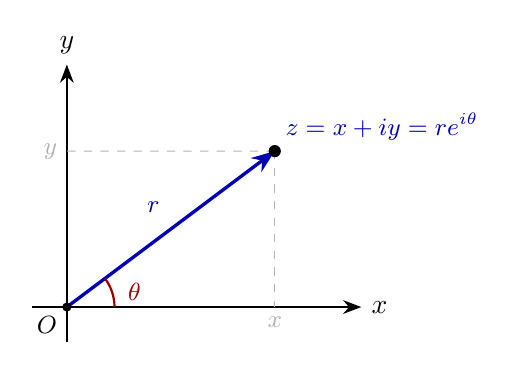
\begin{tikzpicture}[scale=1.1]
  \draw[-Stealth,thick] (-0.4,0)--(3.4,0) node[right]{$x$};
  \draw[-Stealth,thick] (0,-0.4)--(0,2.8) node[above]{$y$};
  \coordinate (O) at (0,0);
  \coordinate (Z) at (2.4,1.8);
  \coordinate (X) at (2.4,0);
  % 向量
  \draw[-Stealth,very thick,blue!70!black] (O)--(Z)
    node[above right,font=\small]{$z=x+iy=re^{i\theta}$};
  % 投影虚线
  \draw[dashed,gray!60] (Z)--(X) node[below,font=\small]{$x$};
  \draw[dashed,gray!60] (Z)--(0,1.8) node[left,font=\small]{$y$};
  % 角度弧
  \draw[red!60!black,thick] (0.55,0) arc[start angle=0,end angle=36.87,radius=0.55];
  \node[red!60!black,font=\small] at (0.78,0.18) {$\theta$};
  % r 标注
  \node[blue!60!black,font=\small] at (1.0,1.15) {$r$};
  % 原点
  \fill (O) circle (1.5pt) node[below left,font=\small]{$O$};
  \fill (Z) circle (2pt);
\end{tikzpicture}
\caption{复平面（Argand 图）：$z=x+iy$ 对应点 $(x,y)$，
  模 $r=|z|$，辐角 $\theta=\arg z$。}
\label{fig:argand}
\end{figure}

\subsection{共轭与模}

$z=x+iy$ 的\textbf{共轭}定义为 $\bar{z}=x-iy$（关于实轴的对称点）。
共轭的基本性质：
\begin{align}
  z+\bar{z} &= 2\re{z}, & z-\bar{z} &= 2i\,\im{z}, \\
  z\bar{z} &= |z|^2, & |\bar{z}| &= |z|.
\end{align}

模的基本性质（$z,w\in\CC$）：
\begin{align}
  |zw| &= |z||w|, &
  \left|\frac{z}{w}\right| &= \frac{|z|}{|w|}, &
  |z+w| &\le |z|+|w|. \quad\text{（三角不等式）}
\end{align}

\subsection{四则运算}

设 $z_1=x_1+iy_1$，$z_2=x_2+iy_2$。

\textbf{加减法：}
\begin{equation}
  z_1\pm z_2 = (x_1\pm x_2) + i(y_1\pm y_2).
  \label{eq:add}
\end{equation}

\textbf{乘法：}
\begin{equation}
  z_1 z_2 = (x_1 x_2 - y_1 y_2) + i(x_1 y_2 + x_2 y_1).
  \label{eq:mul}
\end{equation}
用指数形式更直观：若 $z_j=r_j e^{i\theta_j}$，则
\begin{equation}
  z_1 z_2 = r_1 r_2\,e^{i(\theta_1+\theta_2)}.
  \label{eq:mul_exp}
\end{equation}
即\textbf{模相乘，辐角相加}。

\textbf{除法：}利用共轭有理化
\begin{equation}
  \frac{z_1}{z_2} = \frac{z_1\bar{z}_2}{|z_2|^2}
  = \frac{(x_1 x_2+y_1 y_2)+i(x_2 y_1-x_1 y_2)}{x_2^2+y_2^2},
  \quad z_2\ne0.
  \label{eq:div}
\end{equation}
用指数形式：$\frac{z_1}{z_2}=\frac{r_1}{r_2}\,e^{i(\theta_1-\theta_2)}$，即\textbf{模相除，辐角相减}。

\subsection{乘方与开方}

\textbf{De Moivre 公式：}对正整数 $n$，
\begin{equation}
  z^n = r^n(\cos n\theta + i\sin n\theta) = r^n e^{in\theta}.
  \label{eq:demoivre}
\end{equation}

\textbf{$n$ 次方根：}方程 $w^n=z$（$z\ne0$，$n\in\ZZ^+$）有恰好 $n$ 个解：
\begin{equation}
  w_k = r^{1/n}\exp\!\left(i\frac{\theta+2k\pi}{n}\right),
  \quad k=0,1,\ldots,n-1.
  \label{eq:nthroot}
\end{equation}
这 $n$ 个根均匀分布在以原点为圆心、$r^{1/n}$ 为半径的圆上。

\subsection{初等复数函数}

\textbf{指数函数：}$e^z=e^x(\cos y+i\sin y)$，满足 $|e^z|=e^x$，$\arg(e^z) \equiv y \pmod{2\pi}$。

\textbf{三角函数：}
\begin{align}
  \cos z &= \frac{e^{iz}+e^{-iz}}{2}, &
  \sin z &= \frac{e^{iz}-e^{-iz}}{2i}.
  \label{eq:trig}
\end{align}

\textbf{对数函数（多值与主支）：}
\[
  \log z=\ln|z|+i\arg z
\]
为多值；取主辐角 $\Arg z\in(-\pi,\pi]$ 得\textbf{主值支}
\[
  \Log z=\ln|z|+i\Arg z,
\]
在割线平面 $\CC\setminus(-\infty,0]$ 上全纯。
沿负实轴绕 $0$ 一周，$\arg$ 跳 $2\pi$，故 $z=0$（及 $\infty$）为\textbf{分支点}。
后文 Hankel 围道、$(-z)^{s-1}$ 等均在固定一支后讨论（第~\ref{ch:gamma_function}~、\ref{ch:riemann_zeta_continuation}~章）。

%================================================================
\section{解析函数}
%================================================================

\subsection{复变函数的极限与连续性}

为了严格定义极限，先引入复平面上点集的\textbf{聚点}概念：
设 $E \subset \CC$，$z_0 \in \CC$。若对任意 $\delta > 0$，去心邻域
$0 < |z-z_0| < \delta$ 内都含有 $E$ 中的点，则称 $z_0$ 是 $E$ 的一个聚点
（也称极限点或累积点）。这等价于：存在 $E \setminus \{z_0\}$ 中的互异点列
$\{z_n\}$ 使得 $\lim_{n \to \infty} z_n = z_0$。

设 $f:D\to\CC$（$D\subset\CC$），$z_0$ 是 $D$ 的聚点。若
\[
  \forall\,\varepsilon>0,\;\exists\,\delta>0,\;\forall\,z\in D,\;0<|z-z_0|<\delta
  \;\Rightarrow\; |f(z)-A|<\varepsilon,
\]
则称 $A=\lim_{z\to z_0}f(z)$。
注意：复平面中 $z\to z_0$ 可沿任意路径趋近，
这比实数情形强得多。

\subsection{复导数与 Cauchy--Riemann 方程}

\begin{definition}{复导数}{}
\label{def:complex_deriv}
若极限
\begin{equation}
  f'(z_0) = \lim_{\Delta z\to 0}\frac{f(z_0+\Delta z)-f(z_0)}{\Delta z}
  \label{eq:complex_deriv}
\end{equation}
存在（且与 $\Delta z\to0$ 的路径无关），则称 $f$ 在 $z_0$ \textbf{可微}，
$f'(z_0)$ 称为 $f$ 在 $z_0$ 的\textbf{复导数}。
\end{definition}

令 $f(z)=u(x,y)+iv(x,y)$（$u,v:\RR^2\to\RR$），
$z_0=x_0+iy_0$。

\begin{theorem}{Cauchy--Riemann 方程}{}
\label{thm:CR}
令 $f=u+iv$，$z_0=x_0+iy_0$。C-R 方程的充分必要条件应分两侧叙述：
\begin{enumerate}
  \item \textbf{必要性：} 若 $f$ 在 $z_0$ 复可微，且偏导数 $\frac{\partial u}{\partial x}$ 等在该点存在，
  则 $u,v$ 满足
\begin{equation}
    \frac{\partial u}{\partial x} = \frac{\partial v}{\partial y},
    \qquad
    \frac{\partial u}{\partial y} = -\frac{\partial v}{\partial x}.
  \label{eq:CR}
\end{equation}
  （必要性不要求偏导连续。）
  \item \textbf{充分性：} 若 $u,v$ 在 $(x_0,y_0)$ 处\textbf{实可微}（或邻域内偏导存在且在该点连续）
  且满足 C-R 方程，则 $f$ 在 $z_0$ 复可微，且
  $f'(z_0)=\frac{\partial u}{\partial x}+i\frac{\partial v}{\partial x}
  =\frac{\partial v}{\partial y}-i\frac{\partial u}{\partial y}$。
\end{enumerate}
\end{theorem}

\begin{proof}
令 $\Delta z = \Delta x + i\Delta y$。

\textbf{必要性。} 沿实轴方向（$\Delta y=0$，$\Delta z=\Delta x$）：
\begin{align}
  f'(z_0) &= \lim_{\Delta x\to0}\frac{f(z_0+\Delta x)-f(z_0)}{\Delta x}
  = \frac{\partial u}{\partial x}+i\frac{\partial v}{\partial x}.
\end{align}
沿虚轴方向（$\Delta x=0$，$\Delta z=i\Delta y$）：
\begin{align}
  f'(z_0) &= \lim_{\Delta y\to0}\frac{f(z_0+i\Delta y)-f(z_0)}{i\Delta y}
  = \frac{1}{i}\!\left(\frac{\partial u}{\partial y}+i\frac{\partial v}{\partial y}\right)
  = \frac{\partial v}{\partial y}-i\frac{\partial u}{\partial y}.
\end{align}
两种路径极限相等，得式~\eqref{eq:CR}。

\textbf{充分性。} 若 C-R 成立且 $u,v$ 在该点实可微，则可验证差商极限与路径无关（标准估计），故 $f'(z_0)$ 存在。
\end{proof}

\subsection{解析函数的定义}

\begin{definition}{解析函数}{}
\label{def:analytic}
若 $f$ 在 $z_0$ 的某邻域内每点均可微，
则称 $f$ 在 $z_0$ \textbf{解析}（全纯，holomorphic）。
若 $f$ 在区域 $D$ 内每点均解析，则称 $f$ 为 $D$ 上的\textbf{解析函数}（全纯函数）。
若 $f$ 在整个复平面 $\CC$ 上解析，则称 $f$ 为\textbf{整函数}（entire function）。
\end{definition}


「在一点可微」与「在一点解析」的区别：解析要求在邻域内处处可微，
而可微只要求该点本身，故解析更强。

% 整框不跨页（empty+borderline 跨页时框线易缺）；页末空间不足则整框移到下页
\begin{theorem}[breakable=false]{恒等定理}{}
\label{thm:identity}
设 $D\subset\CC$ 为\textbf{连通}区域，$f$ 在 $D$ 内全纯。
若零点集 $\{z\in D:f(z)=0\}$ 在 $D$ 内有聚点，则 $f\equiv 0$ 于 $D$。
等价地：若 $f,g$ 在 $D$ 内全纯，且在某有聚点的子集 $E\subset D$ 上 $f=g$，则 $f\equiv g$ 于 $D$。
\end{theorem}

\begin{proof}[证明提要]
设 $Z=\{f=0\}$ 在 $D$ 内有聚点 $z_*$。由幂级数展开，若 $f\not\equiv 0$，则零点孤立，
与 $z_*$ 为聚点矛盾。连通性将「在一点邻域恒零」传到全 $D$。
\end{proof}

后文解析延拓的唯一性（第~\ref{ch:analytic_continuation_general}~章）以本定理为根；
Schwarz 反射等论证中「在实轴上一致则延拓唯一」亦依赖它。

\label{def:meromorphic}
设 $D\subset\CC$ 为区域。若 $f$ 在 $D$ 内除若干\textbf{极点}外处处全纯
（每个极点为孤立奇点，且为有限阶极点，见第~\ref{sec:singularity}~节），
则称 $f$ 在 $D$ 上\textbf{亚纯}（meromorphic）。
例如有理函数，以及第~\ref{ch:riemann_zeta_continuation}~章解析延拓后的 $\zeta(s)$
（仅 $s=1$ 为极点）在 $\CC$ 上亚纯。
幅角原理对亚纯函数陈述（零点与极点计重数）。

\subsection{调和函数}

\label{thm:harmonic}
若 $f=u+iv$ 在 $D$ 内解析，则 $u,v$ 均满足 Laplace 方程：
\begin{equation}
  \nabla^2 u = \frac{\partial^2 u}{\partial x^2}+\frac{\partial^2 u}{\partial y^2}=0,
  \qquad
  \nabla^2 v = 0.
  \label{eq:laplace}
\end{equation}
此时称 $u,v$ 为\textbf{调和函数}，$v$ 称为 $u$ 的\textbf{共轭调和函数}。
（由 C-R 方程~\eqref{eq:CR} 对 $x$、$y$ 分别求导并相加即得；偏导可交换。）

\subsection{常见整函数与奇点}

\begin{center}
\renewcommand{\arraystretch}{1.7}
\begin{tabular}{lll}
\toprule
函数 & 解析区域 & 奇点 \\
\midrule
多项式 $P(z)$ & 全平面 $\CC$（整函数） & 无 \\
$e^z,\sin z,\cos z$ & 全平面 $\CC$（整函数） & 无 \\
$1/z$ & $\CC\setminus\{0\}$ & $z=0$（单极点）\\
$1/(z^2+1)$ & $\CC\setminus\{\pm i\}$ & $z=\pm i$（单极点）\\
$\Log z$ & $\CC\setminus(-\infty,0]$ & $z=0, \infty$（分支点）\\
$e^{1/z}$ & $\CC\setminus\{0\}$ & $z=0$（本性奇点）\\
\bottomrule
\end{tabular}
\end{center}


%================================================================
\subsection{保角映射}\label{sec:conformal}
%================================================================

\label{def:conformal}
设 $f:D\to\CC$ 在区域 $D$ 内解析。
若 $f$ 在点 $z_0\in D$ 处满足 $f'(z_0)\ne0$，
则称 $f$ 在 $z_0$ 处是\textbf{保角的}（conformal）；
若在 $D$ 内每点均保角，则称 $f$ 为 $D$ 上的\textbf{保角映射}。

\paragraph{保角性的几何含义}
设两条光滑曲线 $\gamma_1,\gamma_2$ 在 $z_0$ 处相交，
夹角（切线方向之差）为 $\theta$。
若 $f'(z_0)\ne0$，则 $f(\gamma_1)$ 与 $f(\gamma_2)$
在 $w_0=f(z_0)$ 处的夹角仍为 $\theta$（且方向不变）。
在 $f'(z_0)\ne0$ 处，$f$ 的局部作用是旋转角 $\arg f'(z_0)$、
放大倍率 $|f'(z_0)|$，即\textbf{旋转加等比放大}，从而保角。
\label{thm:conformal}
更完整地说：设 $f$ 在区域 $D$ 内解析。
若 $f'(z_0)\ne0$，则 $f$ 在 $z_0$ 处保角；
若 $f'(z_0)=0$，则不保角——角度被放大为原来的 $m$ 倍，其中
$m\ge 2$ 是 $f(z)-f(z_0)$ 在 $z_0$ 处的零点阶数。
（设曲线 $\gamma$ 过 $z_0$、切方向 $e^{i\varphi}$，则像曲线切方向为
$|f'(z_0)|\,e^{i(\varphi+\arg f'(z_0))}$，旋转角与 $\gamma$ 的选取无关。）

$\zeta(s)$ 作为全纯映射在 $\zeta'\ne0$ 处局部保角；
与临界线、零点、极点同框的几何示意见第~\ref{ch:visualization}~章
（§\ref{sec:conformal_global}），这里无需赘述。

%================================================================
\subsection{Schwarz 反射原理}\label{sec:schwarz_reflection}
%================================================================

\label{thm:schwarz_reflection}
\textbf{Schwarz 反射原理}（Schwarz Reflection Principle）
是解析函数的一类对称延拓：若函数在实轴上取实值，则上半平面的解析函数可
关于实轴按共轭延拓到下半平面。
设 $D^+$ 是上半平面 $\operatorname{Im}(z)>0$ 中的区域，
$I$ 是 $D^+$ 的边界与实轴相交的一段开区间，
$D^- = \{\bar{z}: z\in D^+\}$ 是 $D^+$ 关于实轴的对称区域。
若 $f$ 在 $D^+$ 内解析，在 $I$ 上连续且取\textbf{实值}
（即 $\operatorname{Im}f(x)=0$ 对所有 $x\in I$），
则 $f$ 可延拓为在 $D^+\cup I\cup D^-$ 上的解析函数，
\begin{equation}
    f(\bar{z}) = \overline{f(z)}, \qquad z\in D^+\cup I\cup D^-.
  \label{eq:schwarz_reflection}
\end{equation}
证明思路：在 $D^-$ 上令 $g(z)=\overline{f(\bar{z})}$，由 C-R 知 $g$ 解析；
在 $I$ 上 $f$ 取实值故 $f=g$；由恒等定理~\ref{thm:identity}
（及第~\ref{ch:analytic_continuation_general}~章的延拓唯一性）得整体延拓。
更一般地，反射轴不必是实轴，圆弧或直线段亦可；
若 $f$ 将曲线 $\mathcal{C}$ 映到 $\mathcal{C}'$，则可关于二者联合延拓。

对黎曼 $\zeta$ 函数：在 $\operatorname{Re}s>1$ 上由实系数 Dirichlet 级数取实值，
从而由本原理得共轭对称 $\zeta(\bar{s})=\overline{\zeta(s)}$。
完整陈述与证明见第~\ref{ch:riemann_zeta_intro}~章第~\ref{sec:schwarz}~节。

%================================================================
\section{Cauchy 积分理论}
%================================================================


\subsection{复积分的定义}

设 $\mathcal{C}$ 是复平面中从 $a$ 到 $b$ 的光滑曲线，
参数化为 $z(t)=x(t)+iy(t)$（$t\in[\alpha,\beta]$），
$f$ 在 $\mathcal{C}$ 上连续。沿 $\mathcal{C}$ 的\textbf{复积分}定义为
\begin{equation}
  \int_{\mathcal{C}} f(z)\dif z
  = \int_\alpha^\beta f(z(t))\,z'(t)\dif t.
  \label{eq:complex_int}
\end{equation}
若 $f=u+iv$，$\dif z=\dif x+i\dif y$，则等价地：
\begin{equation}
  \int_{\mathcal{C}} f\dif z
  = \int_{\mathcal{C}}(u\dif x-v\dif y)
  + i\int_{\mathcal{C}}(v\dif x+u\dif y).
  \label{eq:complex_int2}
\end{equation}

\textbf{基本估计（ML 不等式）：}
\begin{equation}
  \left|\int_{\mathcal{C}} f(z)\dif z\right|
  \le \max_{z\in\mathcal{C}}|f(z)|\cdot L(\mathcal{C}),
  \label{eq:ML}
\end{equation}
其中 $L(\mathcal{C})$ 是曲线 $\mathcal{C}$ 的弧长。

\subsection{Cauchy 积分定理}

\begin{theorem}{Cauchy 积分定理}{}
\label{thm:cauchy_theorem}
设 $f$ 在单连通区域 $D$ 内解析，$\mathcal{C}$ 是 $D$ 内任意一条简单闭曲线（正向），则
\begin{equation}
    \oint_{\mathcal{C}} f(z)\dif z = 0.
  \label{eq:cauchy_theorem}
\end{equation}
\end{theorem}

\begin{proof}[证明（Green 公式法；$f'\in C^0$ 情形）]
设 $\mathcal{C}$ 围成区域 $G\subset D$。令 $f=u+iv$，
并\textbf{额外假定} $u,v$ 在 $G$ 的闭包上属于 $C^1$（等价于 $f'$ 连续时成立）。
仅“邻域内复可微”而不假设 $f'$ 连续时，需用 Goursat 定理去掉连续性假设，此处不展开。
由式~\eqref{eq:complex_int2}：
\begin{align}
  \oint_{\mathcal{C}} f\dif z
  &= \oint_{\mathcal{C}}(u\dif x-v\dif y)
   + i\oint_{\mathcal{C}}(v\dif x+u\dif y).
\end{align}

对每个实线积分用 Green 公式（$\oint_{\mathcal{C}}P\dif x+Q\dif y
=\iint_G(\frac{\partial Q}{\partial x}-\frac{\partial P}{\partial y})\dif x\dif y$）：
\begin{align}
  \oint_{\mathcal{C}}(u\dif x-v\dif y)
  &= \iint_G\!\left(-\frac{\partial v}{\partial x}-\frac{\partial u}{\partial y}\right)\dif x\dif y = 0,\\
  \oint_{\mathcal{C}}(v\dif x+u\dif y)
  &= \iint_G\!\left(\frac{\partial u}{\partial x}-\frac{\partial v}{\partial y}\right)\dif x\dif y = 0,
\end{align}
两个被积函数均由 C-R 方程~\eqref{eq:CR} 为零。
\end{proof}

由此，若 $f$ 在单连通区域 $D$ 内解析，则 $\int_{\mathcal{C}}f(z)\dif z$
的值只与端点 $a,b$ 有关，与连接 $a,b$ 的路径 $\mathcal{C}\subset D$ 无关。

\subsection{Cauchy 积分公式}

\begin{theorem}{Cauchy 积分公式}{}
\label{thm:cauchy_formula}
设 $f$ 在区域 $D$ 内解析，$\mathcal{C}$ 是 $D$ 内围绕点 $z_0$
的简单正向闭曲线（$z_0$ 在 $\mathcal{C}$ 内部），则
\begin{equation}
    f(z_0) = \frac{1}{2\pi i}\oint_{\mathcal{C}}\frac{f(z)}{z-z_0}\dif z.
  \label{eq:cauchy_formula}
\end{equation}
\end{theorem}

\begin{proof}
由 Cauchy 定理，可将 $\mathcal{C}$ 变形为以 $z_0$ 为圆心、半径 $\varepsilon>0$ 的小圆 $C_\varepsilon$：
\begin{equation}
  \oint_{\mathcal{C}}\frac{f(z)}{z-z_0}\dif z
  = \oint_{C_\varepsilon}\frac{f(z)}{z-z_0}\dif z.
  \label{eq:CF_step1}
\end{equation}

参数化 $z=z_0+\varepsilon e^{i\theta}$（$\theta:0\to2\pi$），
$\dif z=i\varepsilon e^{i\theta}\dif\theta$：
\begin{align}
  \oint_{C_\varepsilon}\frac{f(z)}{z-z_0}\dif z
  &= \int_0^{2\pi}\frac{f(z_0+\varepsilon e^{i\theta})}{\varepsilon e^{i\theta}}
     \cdot i\varepsilon e^{i\theta}\dif\theta
  = i\int_0^{2\pi} f(z_0+\varepsilon e^{i\theta})\dif\theta.
  \label{eq:CF_step2}
\end{align}

令 $\varepsilon\to0$，由 $f$ 的连续性，被积函数一致趋于 $f(z_0)$：
\begin{equation}
  \lim_{\varepsilon\to0}\oint_{C_\varepsilon}\frac{f(z)}{z-z_0}\dif z
  = i\int_0^{2\pi}f(z_0)\dif\theta = 2\pi i\,f(z_0). \qedhere
\end{equation}
\end{proof}


Cauchy 积分公式是复分析中的核心结果之一：
它表明，若已知 $f$ 在闭曲线 $\mathcal{C}$ 上的值，
则可以确定 $f$ 在 $\mathcal{C}$ 内部每一点的值。
这体现了解析函数的"刚性"（rigidity）——边界值完全决定内部。


\subsection{高阶导数公式}

\label{thm:cauchy_higher}
在定理~\ref{thm:cauchy_formula} 的条件下，$f$ 在 $z_0$ 处具有任意阶导数，且
\begin{equation}
    f^{(n)}(z_0) = \frac{n!}{2\pi i}\oint_{\mathcal{C}}\frac{f(z)}{(z-z_0)^{n+1}}\dif z,
    \quad n=0,1,2,\ldots
  \label{eq:cauchy_higher}
\end{equation}
（对式~\eqref{eq:cauchy_formula} 关于 $z_0$ 在积分号下求导即得。）

\subsection{含参量积分与全纯级数}
\label{sec:param_integral}

后文 $\Gamma$、Mellin 与 $\zeta$ 的积分表示均依赖「对参数全纯」的含参量积分。
\label{thm:param_integral}
设 $\Omega\subset\CC$ 为区域，$I\subset\RR$ 为区间（可无界），
$F:\Omega\times I\to\CC$ 满足：
\begin{enumerate}
  \item 对几乎处处的 $t\in I$，$s\mapsto F(s,t)$ 在 $\Omega$ 内全纯；
  \item 对每个紧集 $K\subset\Omega$，存在可积控制 $g_K(t)$，使
        $|F(s,t)|\le g_K(t)$ 对一切 $s\in K$、$t\in I$ 成立，
        且 $\int_I g_K<\infty$。
\end{enumerate}
则 $\Phi(s)=\int_I F(s,t)\,\mathrm{d}t$ 在 $\Omega$ 内全纯，且可在积分号下求导：
$\Phi'(s)=\int_I \frac{\partial F}{\partial s}\,\mathrm{d}t$。
（紧集上由控制收敛；或对小三角形用 Morera 定理。）

\label{thm:weierstrass_series}
同样，若 $f_n$ 在区域 $\Omega$ 内全纯，且 $\sum f_n$ 在 $\Omega$ 的每个紧子集上一致收敛，
则和函数 $f=\sum f_n$ 在 $\Omega$ 内全纯，且可逐项求导
（Weierstrass 全纯函数项级数定理）。
因而 Dirichlet 级数、Euler 乘积的局部一致收敛段给出全纯函数
（第~\ref{ch:riemann_zeta_intro}~章）；
$\Gamma(s)=\int_0^\infty t^{s-1}e^{-t}\,\mathrm{d}t$（$\operatorname{Re}s>0$）
的全纯性即上述含参量积分的直接应用（第~\ref{ch:gamma_function}~章）。

\subsection{Taylor 展开与 Laurent 展开}

若 $f$ 在圆盘 $|z-z_0|<R$ 内解析，则有 \textbf{Taylor 展开}
\begin{equation}
  f(z) = \sum_{n=0}^\infty a_n(z-z_0)^n,
  \quad a_n = \frac{f^{(n)}(z_0)}{n!}
  = \frac{1}{2\pi i}\oint_{\mathcal{C}}\frac{f(z)}{(z-z_0)^{n+1}}\dif z,
  \label{eq:taylor}
\end{equation}
级数在 $|z-z_0|<R$ 内绝对收敛。

%================================================================
\section{Laurent 级数}
%================================================================

\subsection{Laurent 级数的定义}

Taylor 级数要求函数在圆盘内解析，但实际中函数常在奇点附近出现负幂次项。
Laurent 级数将 Taylor 展开推广到\textbf{圆环域}，允许含有负幂次。

\label{def:laurent}
形如
\begin{equation}
  \sum_{n=-\infty}^{+\infty} c_n(z-z_0)^n
  = \cdots + \frac{c_{-2}}{(z-z_0)^2} + \frac{c_{-1}}{z-z_0}
  + c_0 + c_1(z-z_0) + c_2(z-z_0)^2 + \cdots
  \label{eq:laurent_series_def}
\end{equation}
的级数称为以 $z_0$ 为中心的 \textbf{Laurent 级数}，其中 $c_n\in\CC$。
它由\textbf{解析部分} $\sum_{n=0}^{+\infty}c_n(z-z_0)^n$
与\textbf{主部} $\sum_{n=1}^{+\infty}c_{-n}(z-z_0)^{-n}$ 组成；
当两部分收敛域有交叉（$r<R$）时，级数在圆环 $r<|z-z_0|<R$ 内收敛。
%=========================================
\begin{figure}[ht]
\centering
\begin{tikzpicture}[scale=1.05]

 % 外圆
  \draw[blue!60!black, very thick] (0,0) circle (2.2cm);
  \node[blue!60!black, font=\small] at (2.6,1.55) {$|z-z_0|=R$};
  % 内圆
  \draw[red!60!black, very thick] (0,0) circle (1.0cm);
  \node[red!60!black, font=\small] at (3.0,-0.55) {$|z-z_0|=r$};
     % 圆环阴影
  \begin{scope}
    \clip (0,0) circle (2.2cm);
    \fill[blue!8] (0,0) circle (2.2cm);
    \fill[white] (0,0) circle (1.0cm);
  \end{scope}
  \draw[-Stealth,thick] (-2.8,0)--(2.8,0) node[right,font=\small]{$x$};
  \draw[-Stealth,thick] (0,-2.6)--(0,2.8) node[above,font=\small]{$y$};

  % 中心点（奇点）
  \fill[red] (0,0) circle (2.5pt);
  \node[below right, font=\small, red] at (-0.05,-0.48) {$z_0$（奇点）};
  % 积分曲线
  \draw[purple!70!black, thick,
    decoration={markings, mark=at position 0.25 with {\arrow[scale=1.2]{Stealth}},
                          mark=at position 0.75 with {\arrow[scale=1.2]{Stealth}}},
    postaction={decorate}]
    (0,0) circle (1.55cm);
  \node[purple!70!black, font=\small] at (-1.3,1.1) {$\mathcal{C}$};
  % 收敛区域标注
  \node[font=\small, blue!50!black] at (2.0,2.55)
    {Laurent 级数收敛域};
  % 指示箭头调整：箭头端移动到 C 圈（1.55cm）和外圆（2.2cm）的圆环中部（约1.875cm 半径处）
  \draw[-Stealth, blue!40!black, thin] (2.0,2.42)--(1.34,1.34);
  % r, R 标注
  \draw[<->, blue!70, thin] (0,0)--(0.97,0) node[midway, below, font=\scriptsize]{$r$};
  \draw[<->, blue!70, thin] (0,0)--(2.17,0) node[midway, above, font=\scriptsize]{$R$};
\end{tikzpicture}
\caption{Laurent 级数的收敛域：圆环 $r<|z-z_0|<R$。
  $z_0$ 为奇点，$\mathcal{C}$ 为圆环内用于计算系数的积分曲线。}
\label{fig:laurent_annulus}
\end{figure}
%=======================================
\subsection{Laurent 展开定理及其证明}

\begin{theorem}{Laurent 展开定理}{}
\label{thm:laurent}
设 $f$ 在圆环 $r<|z-z_0|<R$（$0\le r<R\le+\infty$）内解析，
则 $f$ 可唯一地展开为 Laurent 级数：
\begin{equation}
    f(z) = \sum_{n=-\infty}^{+\infty} c_n(z-z_0)^n,
    \quad
    c_n = \frac{1}{2\pi i}\oint_{\mathcal{C}}\frac{f(w)}{(w-z_0)^{n+1}}\dif w,
  \label{eq:laurent}
\end{equation}
其中 $\mathcal{C}$ 是圆环内任意包围 $z_0$ 的简单正向闭曲线，
$n=0,\pm1,\pm2,\ldots$
\end{theorem}

\begin{proof}
设 $z$ 在圆环内，取 $r<r_1<|z-z_0|<r_2<R$。
在圆环 $r_1<|w-z_0|<r_2$ 内，$f$ 解析，$z$ 在此圆环内。

由多连通域的 Cauchy 积分公式：
\begin{equation}
  f(z) = \frac{1}{2\pi i}\oint_{C_{r_2}}\frac{f(w)}{w-z}\dif w
        -\frac{1}{2\pi i}\oint_{C_{r_1}}\frac{f(w)}{w-z}\dif w,
  \label{eq:laurent_proof_1}
\end{equation}
其中 $C_{r_j}$ 为以 $z_0$ 为圆心、半径 $r_j$ 的正向圆。

\textbf{处理外圆 $C_{r_2}$ 上的积分：}
对 $w\in C_{r_2}$，$|z-z_0|<|w-z_0|$，令 $\zeta=\frac{z-z_0}{w-z_0}$，$|\zeta|<1$：
\begin{align}
  \frac{1}{w-z}
  &= \frac{1}{(w-z_0)-(z-z_0)}
  = \frac{1}{w-z_0}\cdot\frac{1}{1-\zeta}
  = \frac{1}{w-z_0}\sum_{n=0}^\infty\zeta^n
  \notag\\
  &= \sum_{n=0}^\infty\frac{(z-z_0)^n}{(w-z_0)^{n+1}}.
  \label{eq:geom_outer}
\end{align}
积分后得解析部分：
\[
\frac{1}{2\pi i}\oint_{C_{r_2}}\frac{f(w)}{w-z}\dif w
 = \sum_{n=0}^\infty c_n(z-z_0)^n,
\]
其中 $c_n=\frac{1}{2\pi i}\oint_{C_{r_2}}\frac{f(w)}{(w-z_0)^{n+1}}\dif w$。

\textbf{处理内圆 $C_{r_1}$ 上的积分：}
对 $w\in C_{r_1}$，$|w-z_0|<|z-z_0|$，令 $\eta=\frac{w-z_0}{z-z_0}$，$|\eta|<1$：
\begin{align}
  \frac{-1}{w-z}
  &= \frac{1}{z-w}
  = \frac{1}{z-z_0}\cdot\frac{1}{1-\eta}
  = \sum_{n=0}^\infty\frac{(w-z_0)^n}{(z-z_0)^{n+1}}.
  \label{eq:geom_inner}
\end{align}
积分后令 $m=-(n+1)$（$m=-1,-2,-3,\ldots$），得主部：
$ -\frac{1}{2\pi i}\oint_{C_{r_1}}\frac{f(w)}{w-z}\dif w
 = \sum_{n=1}^\infty c_{-n}(z-z_0)^{-n}$，
其中 $ c_{-n}=\frac{1}{2\pi i}\oint_{C_{r_1}}\frac{f(w)}{(w-z_0)^{-n+1}}\dif w$。

\textbf{合并：}由 Cauchy 定理，$C_{r_1}$ 和 $C_{r_2}$ 上的积分可以统一为同一围道 $\mathcal{C}$（系数 $c_n$ 与 $r_1,r_2$ 的具体取值无关）。
将两部分合并即得式~\eqref{eq:laurent}。

\textbf{唯一性：}若有两个 Laurent 展开，对差级数逐项积分（利用 $\oint_\mathcal{C}(z-z_0)^n\dif z=2\pi i\cdot\delta_{n,-1}$，其中 $\delta_{ij}$ 为 Kronecker 记号），可证各系数相同。
\end{proof}

\subsection{计算方法与本书用途}

直接用积分求系数 $c_n$ 通常繁琐；常用：
（i）已知 Taylor 级数作代换；（ii）部分分式 + 几何级数
$\frac{1}{1-\zeta}=\sum_{n\ge0}\zeta^n$（$|\zeta|<1$）。

常用手法：已知 Taylor 级数作代换；部分分式配几何级数
$\frac{1}{1-\zeta}=\sum_{n\ge0}\zeta^n$（$|\zeta|<1$）。
同一函数在不同圆环内的 Laurent 展开一般不同，须先固定中心与区域。

本书用 Laurent 展开主要读三件事（细节见下一节）：
\begin{itemize}
  \item \textbf{奇点类型}：主部为空 / 有限 / 无穷 $\Leftrightarrow$ 可去 / 极点 / 本性；
  \item \textbf{留数}：$\Res(f,z_0)=c_{-1}$；本性奇点只能靠展开读 $c_{-1}$；
  \item \textbf{围道积分}：$\oint f=2\pi i\sum c_{-1}$（留数定理）。
\end{itemize}

\label{def:res_infty}
\textbf{无穷远处的留数}定义为
\begin{equation}
  \Res(f,\infty)
  \;=\;
  -\frac{1}{2\pi i}\oint_{|z|=R}f(z)\,\mathrm{d}z
  \;=\;
  -c_{-1}^{(\infty)},
  \label{eq:res_infty}
\end{equation}
其中 $c_{-1}^{(\infty)}$ 来自 $f$ 在 $\infty$ 处（$w=1/z$）的 Laurent 展开。
有限奇点留数与 $\Res(f,\infty)$ 之和为 $0$。

Perron / Laplace 逆变换中的竖线积分，在闭合后亦化为留数和
（第~\ref{ch:integral_transforms}~、\ref{ch:riemann_explicit_formula}~章）；
多阶极点用公式~\eqref{eq:res_mth}，不必在此展开特例。

\subsection{Laurent 与 Taylor 的比较}

\begin{center}
\renewcommand{\arraystretch}{1.5}
\begin{tabular}{lll}
\toprule
 & Taylor & Laurent \\
\midrule
幂次 & $n\ge 0$ & $n\in\ZZ$ \\
收敛域 & 圆盘 & 圆环（中心可有奇点） \\
系数 & $\dfrac{f^{(n)}(z_0)}{n!}$ & 围道积分 \\
\bottomrule
\end{tabular}
\end{center}

%================================================================
\section{孤立奇点与留数}
%================================================================

\subsection{孤立奇点的分类}\label{sec:singularity}

若 $f$ 在 $z_0$ 处不解析，但在某去心邻域 $0<|z-z_0|<\delta$ 内解析，
则称 $z_0$ 为 $f$ 的\textbf{孤立奇点}。
根据 $f$ 在 $z_0$ 处 Laurent 展开的主部，奇点分三类：

\begin{center}
\renewcommand{\arraystretch}{1.9}
\begin{tabular}{lp{4.0cm}p{5.0cm}l}
\toprule
类型 & Laurent 主部 & 等价条件 & 典型例子 \\
\midrule
可去奇点 &
无主部（$c_{-n}=0$，$\forall n\ge1$）&
$\displaystyle\lim_{z\to z_0}f(z)$ 存在有限 &
$\dfrac{\sin z}{z}$ 在 $z=0$ \\[6pt]
$m$ 阶极点 &
$c_{-m}\ne0$，$c_{-n}=0$（$n>m$）&
$\displaystyle\lim_{z\to z_0}(z-z_0)^m f(z)\ne0,\infty$ &
$\dfrac{1}{(z-1)^2}$ 在 $z=1$ \\[6pt]
本性奇点 &
无穷多个非零 $c_{-n}$ &
$\displaystyle\lim_{z\to z_0}f(z)$ 不存在 &
$e^{1/z}$ 在 $z=0$ \\
\bottomrule
\end{tabular}
\end{center}

\subsection{留数的定义}

\begin{definition}{留数}{}
\label{def:residue}
设 $z_0$ 是 $f$ 的孤立奇点，$f$ 在 $z_0$ 处的 Laurent 展开为式~\eqref{eq:laurent}，
则 $f$ 在 $z_0$ 处的\textbf{留数}（残数）定义为 $c_{-1}$：
\begin{equation}
  \Res(f,z_0) = c_{-1} = \frac{1}{2\pi i}\oint_{C_\varepsilon} f(z)\dif z,
  \label{eq:res_def}
\end{equation}
其中 $C_\varepsilon$ 是以 $z_0$ 为圆心的充分小正向圆。
\end{definition}

\subsection{留数的计算方法}

\textbf{方法一：}对简单极点（$m=1$），
\begin{equation}
  \Res(f,z_0) = \lim_{z\to z_0}(z-z_0)f(z).
  \label{eq:res_simple}
\end{equation}

\textbf{方法二：}若 $f(z)=g(z)/h(z)$，$g(z_0)\ne0$，$h(z_0)=0$，$h'(z_0)\ne0$（单零点），
\begin{equation}
  \Res(f,z_0) = \frac{g(z_0)}{h'(z_0)}.
  \label{eq:res_quotient}
\end{equation}

\textbf{方法三：}对 $m$ 阶极点，
\begin{equation}
  \Res(f,z_0) = \frac{1}{(m-1)!}\lim_{z\to z_0}
  \frac{\dif^{m-1}}{\dif z^{m-1}}\!\left[(z-z_0)^m f(z)\right].
  \label{eq:res_mth}
\end{equation}

\textbf{方法四：}对本性奇点，展开 Laurent 级数，直接读取 $c_{-1}$。

\subsection{留数定理}

\begin{theorem}{留数定理}{}
\label{thm:residue}
设 $f$ 在区域 $D$ 内除有限个孤立奇点 $z_1,z_2,\ldots,z_n$ 外处处解析，
$\mathcal{C}$ 是 $D$ 内包含所有奇点的简单正向闭曲线，则
\begin{equation}
    \oint_{\mathcal{C}} f(z)\dif z
    = 2\pi i\sum_{k=1}^n\Res(f,z_k).
  \label{eq:residue_thm}
\end{equation}
\end{theorem}

\begin{proof}
在每个奇点外作小圆，用割线将多连通域化为单连通域，对所得区域用 Cauchy 定理；
割线去回程抵消，小圆积分给出留数。几何与完整推导见图~\ref{fig:residue}。
\end{proof}

% 非浮动：紧接留数定理，固定于幅角定理节之前
\begin{center}
\begin{tikzpicture}[scale=1.15, line width=1.0pt]

%==========================================================
% 基本参数
%==========================================================
\def\Ra{3.6}
\def\Rb{2.4}
\def\rc{0.42}
\def\off{0.14}

\coordinate (O1) at ( 1.00, 1.00);
\coordinate (O2) at ( 1.20, -0.75);
\coordinate (O3) at (-1.80, 0.15);

%==========================================================
% 大椭圆
%==========================================================
\draw[blue!70!black, line width=1.6pt,
  decoration={markings,
    mark=at position 0.10 with {\arrow[scale=1.4,blue!70!black]{Stealth}},
    mark=at position 0.35 with {\arrow[scale=1.4,blue!70!black]{Stealth}},
    mark=at position 0.60 with {\arrow[scale=1.4,blue!70!black]{Stealth}},
    mark=at position 0.85 with {\arrow[scale=1.4,blue!70!black]{Stealth}}},
  postaction={decorate}]
  (0,0) ellipse (\Ra cm and \Rb cm);
\node[blue!70!black, font=\small] at (0,-2.78) {$\mathcal{C}$（正向逆时针）};
\node[gray!55, font=\footnotesize] at (2.85,1.98) {$f$ 解析};

%==========================================================
% 奇点标记
%==========================================================
\fill[red!80!black] (O1) circle (2.2pt)
  node[above=2pt, font=\footnotesize, red!70!black] {$z_1$};
\fill[red!80!black] (O2) circle (2.2pt)
  node[right=3pt, font=\footnotesize, red!70!black] {$z_2$};
\fill[red!80!black] (O3) circle (2.2pt)
  node[above=2pt, font=\footnotesize, red!70!black] {$z_3$};

%==========================================================
% 接触点
%==========================================================
\coordinate (P0) at ({3.6*cos(72)}, {2.4*sin(72)});
\coordinate (P1in) at ({1.00+\rc*cos(80)}, {1.00+\rc*sin(80)});
\coordinate (P1out) at ({1.00+\rc*cos(270)}, {1.00+\rc*sin(270)});
\coordinate (P2in) at ({1.20+\rc*cos(100)}, {-0.75+\rc*sin(100)});
\coordinate (P2out) at ({1.20+\rc*cos(200)}, {-0.75+\rc*sin(200)});
\coordinate (P3) at ({-1.80+\rc*cos(10)}, {0.15+\rc*sin(10)});

%==========================================================
% 手绘割线样式
%==========================================================
\tikzset{
  handdrawn/.style={
    decoration={random steps, segment length=5pt, amplitude=0.7pt},
    decorate, line cap=round
  }
}

%==========================================================
% 侧向双箭头宏
% 旋向分析：路径在小圆上逆时针旋转，从去程方向看
% 圆弧在右侧展开，故：
% 去程箭头 → 放在割线【右侧】（法向 -off）
% 回程箭头 ← 放在割线【左侧】（法向 +off）
% 箭头：open Stealth（空心，带尾巴效果），缩小至 scale=0.82
% 尾巴：在箭头起点处加一小段垂直短线
%==========================================================
\newcommand{\sideArrows}[2]{%
  % 用 pgfgetlastxy 提取割线方向向量
  \pgfpointdiff{\pgfpointanchor{#1}{center}}
               {\pgfpointanchor{#2}{center}}%
  \pgfgetlastxy{\cutdxdim}{\cutdydim}% 保存为带 pt 的 dimension
  \pgfmathsetmacro{\cutdx}{\cutdxdim/1pt}%
  \pgfmathsetmacro{\cutdy}{\cutdydim/1pt}%
  \pgfmathsetmacro{\cutlen}{sqrt(\cutdx*\cutdx+\cutdy*\cutdy)}%
  % 单位法向量（左侧正方向：旋转 +90°）
  \pgfmathsetmacro{\tnx}{-\cutdy/\cutlen}%
  \pgfmathsetmacro{\tny}{ \cutdx/\cutlen}%
  \pgfmathsetmacro{\thalf}{1.65}% 尾巴半长
  % 四个箭头端点
  \coordinate (fwdTail) at ($(#1)!0.40!(#2)!{-\off cm}!90:(#2)$);
  \coordinate (fwdHead) at ($(#1)!0.54!(#2)!{-\off cm}!90:(#2)$);
  \coordinate (bwdTail) at ($(#1)!0.60!(#2)!{ \off cm}!90:(#2)$);
  \coordinate (bwdHead) at ($(#1)!0.46!(#2)!{ \off cm}!90:(#2)$);
  %--- 去程箭头（右侧，A→B）---
  \draw[-{Stealth[scale=0.82, open]}, red!82!black, line width=0.78pt]
    (fwdTail) -- (fwdHead);
  \draw[red!82!black, line width=0.78pt]
    ($(fwdTail)+(\thalf*\tnx pt, \thalf*\tny pt)$)
    -- ($(fwdTail)+(-\thalf*\tnx pt, -\thalf*\tny pt)$);
  %--- 回程箭头（左侧，B→A）---
  \draw[-{Stealth[scale=0.82, open]}, red!82!black, line width=0.78pt]
    (bwdTail) -- (bwdHead);
  \draw[red!82!black, line width=0.78pt]
    ($(bwdTail)+(\thalf*\tnx pt, \thalf*\tny pt)$)
    -- ($(bwdTail)+(-\thalf*\tnx pt, -\thalf*\tny pt)$);
}

%==========================================================
% ① 割线 L0：P0 → P1in
%==========================================================
\draw[red!75!black, line width=1.2pt, handdrawn]
  (P0) to[out=228, in=82, looseness=0.88] (P1in);
\sideArrows{P0}{P1in}
\node[font=\scriptsize, red!60!black] at (1.50,1.86) {$L_0$};

%==========================================================
% ② C1 逆时针：去程 80°→270°，回程 270°→440°
%==========================================================
\draw[red!75!black, line width=1.2pt,
  decoration={markings,
    mark=at position 0.48 with {\arrow[scale=1.05]{Stealth[open]}}},
  postaction={decorate}]
  ({1.00+\rc*cos(80)},{1.00+\rc*sin(80)})
  arc[start angle=80, end angle=270, radius=\rc];

\draw[red!75!black, line width=1.2pt,
  decoration={markings,
    mark=at position 0.52 with {\arrow[scale=1.05]{Stealth[open]}}},
  postaction={decorate}]
  ({1.00+\rc*cos(270)},{1.00+\rc*sin(270)})
  arc[start angle=270, end angle=440, radius=\rc];

\node[font=\footnotesize, red!55!black] at
  ({1.00+(\rc+0.32)*cos(175)},{1.00+(\rc+0.32)*sin(175)}) {$C_1$};

%==========================================================
% ③ 割线 L12：P1out → P2in
%==========================================================
\draw[red!75!black, line width=1.2pt, handdrawn]
  (P1out) to[out=262, in=98, looseness=0.88] (P2in);
\sideArrows{P1out}{P2in}
\node[font=\scriptsize, red!60!black] at
  ({1.00+\rc*cos(270)+0.32},
   {0.5*(1.00+\rc*sin(270)-0.75+\rc*sin(100))}) {$L_{12}$};

%==========================================================
% ④ C2 逆时针：去程 100°→200°，回程 200°→460°
%==========================================================
\draw[red!75!black, line width=1.2pt,
  decoration={markings,
    mark=at position 0.52 with {\arrow[scale=1.05]{Stealth[open]}}},
  postaction={decorate}]
  ({1.20+\rc*cos(100)},{-0.75+\rc*sin(100)})
  arc[start angle=100, end angle=200, radius=\rc];

\draw[red!75!black, line width=1.2pt,
  decoration={markings,
    mark=at position 0.50 with {\arrow[scale=1.05]{Stealth[open]}}},
  postaction={decorate}]
  ({1.20+\rc*cos(200)},{-0.75+\rc*sin(200)})
  arc[start angle=200, end angle=460, radius=\rc];

\node[font=\footnotesize, red!55!black] at
  ({1.20+(\rc+0.32)*cos(330)},{-0.75+(\rc+0.32)*sin(330)}) {$C_2$};

%==========================================================
% ⑤ 割线 L23：P2out → P3
%==========================================================
\draw[red!75!black, line width=1.2pt, handdrawn]
  (P2out) to[out=168, in=345, looseness=0.92] (P3);
\sideArrows{P2out}{P3}
\node[font=\scriptsize, red!60!black] at (-0.32,-0.10) {$L_{23}$};

%==========================================================
% ⑥ C3 逆时针整圈：10°→370°
%==========================================================
\draw[red!75!black, line width=1.2pt,
  decoration={markings,
    mark=at position 0.22 with {\arrow[scale=1.05]{Stealth[open]}},
    mark=at position 0.72 with {\arrow[scale=1.05]{Stealth[open]}}},
  postaction={decorate}]
  ({-1.80+\rc*cos(10)},{0.15+\rc*sin(10)})
  arc[start angle=10, end angle=370, radius=\rc];

\node[font=\footnotesize, red!55!black] at
  ({-1.0+(\rc+0.32)*cos(188)},{-0.32+(\rc+0.32)*sin(188)})
  {$C_3$（整圈）};

%==========================================================
% 出发点
%==========================================================
\fill[blue!70!black] (P0) circle (2.5pt);
\node[blue!60!black, font=\footnotesize, above right] at (P0) {$P_0$};

%==========================================================
% 图例说明框（详细版，椭圆左侧外部）
%==========================================================
\node[draw=gray!45, fill=gray!3, rounded corners=5pt,
  font=\scriptsize, inner sep=8pt, align=left,
  text width=6.0cm] at (-6.65, 0.3)
{%
  \textbf{\normalsize 留数定理（割线法）}\\[5pt]
  %-------- 大围道 --------
  \textbf{大围道 $\mathcal{C}$}（蓝色，逆时针正向）\\
  \quad 简单闭曲线，内含奇点 $z_1,\ldots,z_n$\\
  \quad $f$ 在 $\mathcal{C}$ 及其内部（奇点除外）解析\\[5pt]
  %-------- 割线 --------
  \textbf{割线}（红色手绘曲线，共 $n$ 条）\\
  \quad 无交叉、按序连接各小圆（并连至 $\mathcal{C}$）\\
  \quad 割线将多连通域切割为\\
  \quad 单连通域 $G$，使 Cauchy 定理可用\\[3pt]
  \quad 每条割线沿相同路径走两次：\\[2pt]
  \quad\begin{tikzpicture}[baseline=-1pt]
    \draw[red!80!black,line width=0.75pt]
      (0,0)--(0.6,0);
    \draw[-{Stealth[scale=0.78,open]},red!80!black,line width=0.75pt]
      (0.08,0.10)--(0.28,0.10);
    \draw[red!80!black,line width=0.75pt]
      (0.08,0.14)--(0.08,0.06);
  \end{tikzpicture}
  ~\textbf{去程} $L_k^+$：右侧箭头，\\
  \quad\quad $\mathcal{C}\to C_k$，与逆时针旋向和谐\\[2pt]
  \quad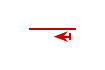
\begin{tikzpicture}[baseline=-1pt]
    \draw[red!80!black,line width=0.75pt]
      (0,0)--(0.6,0);
    \draw[-{Stealth[scale=0.78,open]},red!80!black,line width=0.75pt]
      (0.52,-0.10)--(0.32,-0.10);
    \draw[red!80!black,line width=0.75pt]
      (0.52,-0.06)--(0.52,-0.14);
  \end{tikzpicture}
  ~\textbf{回程} $L_k^-$：左侧箭头，\\
  \quad\quad $C_k\to\mathcal{C}$，方向与去程相反\\[3pt]
  \quad 去回程积分精确抵消（同路反向）：\\
  \quad $\int_{L_k^+}\!\!f\,dz
    +\int_{L_k^-}\!\!f\,dz = 0$\\[5pt]
  %-------- 小圆弧 --------
  \textbf{小圆弧 $C_k$}（红色实线，逆时针 = 正向）\\
  \quad 绕奇点 $z_k$ 作充分小正向圆\\
  \quad 去程弧 $+$ 回程弧 $=$ 逆时针整圈\\
  \quad 两段弧上箭头均沿逆时针方向\\[5pt]
  %-------- 推导 --------
  \textbf{推导}：对单连通域 $G$ 用 Cauchy 定理\\
  \quad $\oint_{\partial G}f\,dz=0$，展开得：\\[2pt]
  \quad $\oint_{\mathcal{C}}\!f\,dz
    +\sum_k\!\Bigl(
      \int_{L_k^+}\!\!+\int_{L_k^-}\Bigr)f\,dz
    -\sum_k\oint_{C_k}\!\!f\,dz=0$\\[3pt]
  \quad 割线项为零。\\
  \quad $\partial G$ 绕每个洞为顺时针，故小圆贡献为
    $-\oint_{C_k}$（$C_k$ 正向）；\\
  \quad 再由
    $\oint_{C_k}f\,dz = 2\pi i\,\mathrm{Res}(f,z_k)$，得：\\[2pt]
  \quad $\oint_{\mathcal{C}}\!f\,dz
    =\sum_{k}\oint_{C_k}\!\!f\,dz$\\[3pt]
  \quad $
    \boxed{\oint_{\mathcal{C}}\!f\,dz
    = 2\pi i\sum_{k}\mathrm{Res}(f,z_k)}$%
};
\end{tikzpicture}
\captionof{figure}{多连通区域割线与留数定理证明示意图（图例内含完整证明）。}
\label{fig:residue}
\end{center}

%================================================================
\section{幅角定理}\label{sec:argument_principle}
%================================================================

\subsection{对数导数与辐角变化}

设 $f$ 在区域 $D$ 内亚纯（除有限个极点外处处解析），
$f$ 在曲线 $\mathcal{C}$ 上无零点也无极点。

恒等式：
\begin{equation}
  \frac{f'(z)}{f(z)} = \frac{\dif}{\dif z}\log f(z)
  = \frac{\dif}{\dif z}\!\left[\ln|f(z)|+i\arg f(z)\right].
  \label{eq:log_deriv}
\end{equation}

在 $f$ 的全纯非零点处上式两端均全纯。
在 $m$ 阶零点处，$f'/f$ 有一阶极点，留数为 $m$；
在 $n$ 阶极点处，$f'/f$ 有一阶极点，留数为 $-n$。
因而沿包围这些点的闭围道积分时，$f'/f$ 的留数之和等于（计重数的）零点个数减去极点个数；
这正是下一小节幅角定理的内容。

沿 $\mathcal{C}$ 积分：
\begin{align}
  \oint_{\mathcal{C}}\frac{f'(z)}{f(z)}\dif z
  &= \Delta_{\mathcal{C}}\ln|f(z)| + i\,\Delta_{\mathcal{C}}\arg f(z).
  \label{eq:log_deriv_int}
\end{align}

若 $\mathcal{C}$ 是闭曲线，$|f(z)|$ 回到原值，故 $\Delta_{\mathcal{C}}\ln|f|=0$，
\begin{equation}
  \oint_{\mathcal{C}}\frac{f'(z)}{f(z)}\dif z = i\,\Delta_{\mathcal{C}}\arg f(z).
  \label{eq:arg_change}
\end{equation}

\subsection{幅角定理（辐角原理）}

\begin{theorem}{幅角定理 / 辐角原理}{}
\label{thm:argument_principle}
设 $f$ 在区域 $D$ 内亚纯，$\mathcal{C}$ 是 $D$ 内的简单正向闭曲线，
$f$ 在 $\mathcal{C}$ 上无零点也无极点。
设 $\mathcal{C}$ 内部 $f$ 的零点个数为 $Z$（计重数），极点个数为 $P$（计重数），则
\begin{equation}
    \frac{1}{2\pi i}\oint_{\mathcal{C}}\frac{f'(z)}{f(z)}\dif z = Z - P.
  \label{eq:argument_principle}
\end{equation}
等价地，
\begin{equation}
  Z - P = \frac{1}{2\pi}\Delta_{\mathcal{C}}\arg f(z).
  \label{eq:argument_principle2}
\end{equation}
\end{theorem}

\begin{proof}
对 $f$ 的每个零点 $a$（$m_a$ 阶）和极点 $b$（$n_b$ 阶），
在附近展开：
\begin{align}
  &a\text{ 处：}\; f(z)=(z-a)^{m_a}g(z),\;g(a)\ne0
  \;\Rightarrow\; \frac{f'}{f}=\frac{m_a}{z-a}+\frac{g'}{g},\\
  &b\text{ 处：}\; f(z)=(z-b)^{-n_b}h(z),\;h(b)\ne0
  \;\Rightarrow\; \frac{f'}{f}=\frac{-n_b}{z-b}+\frac{h'}{h}.
\end{align}

因此 $f'/f$ 在 $\mathcal{C}$ 内部的留数之和为
$\sum_a m_a - \sum_b n_b = Z-P$。
换言之：$f'/f$ 的极点恰好位于 $f$ 的零点与极点处，留数分别为零点阶与极点阶的相反数。
由留数定理：
\[
  \frac{1}{2\pi i}\oint_{\mathcal{C}}\frac{f'}{f}\dif z = Z-P.
\]
结合式~\eqref{eq:arg_change} 即得式~\eqref{eq:argument_principle2}。
\end{proof}

\begin{figure}[ht]
\centering
\begin{tikzpicture}[scale=1.0]
  \begin{scope}[xshift=-4.3cm]
    % z 平面
    \draw[-Stealth,thick] (-2.5,0)--(2.5,0) node[right,font=\small]{$x$};
    \draw[-Stealth,thick] (0,-2.0)--(0,2.0) node[above,font=\small]{$y$};
    \node[font=\small, above left] at (-1.6,1.5) {$z$ 平面};
    % 围道（在1.2倍基础上再×1.3，最终1.56倍：1.68×1.3=2.184cm，1.32×1.3=1.716cm）
    \draw[blue!70!black, very thick, marrow=0.10, marrow=0.35, marrow=0.60, marrow=0.85]
      (0,0) ellipse (2.184cm and 1.716cm);
    % 标注位置再次微调（-1.44×1.3=-1.872cm）
    \node[blue!70!black, font=\small, below] at (0,-1.9) {$\mathcal{C}$};
    % 零点（位置不变）
    \fill[green!60!black] (-1.1,0.7) circle (2.5pt)
      node[above right, font=\scriptsize]{$a_1$零点};
    \fill[green!60!black] (0.5,-0.2) circle (2.5pt)
      node[below right, font=\scriptsize]{$a_2$零点};
    % 极点（位置不变）
    \fill[red] (-0.4,-0.7) circle (2.5pt)
      node[below right, font=\scriptsize]{$b_1$极点};
  \end{scope}

  % 箭头（位置不变）
  \draw[-Stealth, very thick, purple!70!black] (-1.3,0)--(1.6,0)
    node[above, midway, font=\small]{$w=f(z)$};

  \begin{scope}[xshift=4.0cm]
    % w 平面
    \draw[-Stealth,thick] (-2.2,0)--(2.3,0) node[right,font=\small]{$\operatorname{Re}w$};
    \draw[-Stealth,thick] (0,-2.0)--(0,2.0) node[above,font=\small]{$\operatorname{Im}w$};
    \node[font=\small, above left] at (-1.6,1.5) {$w$ 平面};
    % 像曲线 f(C)（在1.2倍基础上再×1.3，所有坐标点最终放大1.56倍）
    \draw[red!70!black, very thick,
      marrow=0.08, marrow=0.33, marrow=0.58, marrow=0.83]
      plot[smooth, tension=0.8]
      coordinates{(1.56,0.468)(0.468,1.716)(-1.404,0.936)(-1.716,-0.468)(0,-1.56)
                  (1.404,-0.78)(1.716,0.156)(0.468,1.56)(-1.248,0.78)(-1.56,-0.624)
                  (0,-1.404)(1.404,-0.624)(1.56,0.468)};
    \fill[black] (0,0) circle (2.5pt) node[below right, font=\small]{$w=0$};
    % 标注位置再次微调（1.32×1.3=1.716, 0.36×1.3=0.468）
    \node[red!70!black, font=\small, right] at (1.716,0.468)
      {$f(\mathcal{C})$};
    % 文字标注位置不变
    \node[font=\small, below] at (0,-1.9)
      {绕原点 $Z-P=1$ 圈};
  \end{scope}
\end{tikzpicture}
\end{figure}

\subsection{几何解释}

幅角定理有直观的几何含义：

当 $z$ 沿正向闭曲线 $\mathcal{C}$ 走一圈时，$w=f(z)$ 描绘出 $w$ 平面中的一条闭曲线 $\Gamma=f(\mathcal{C})$。
$\frac{1}{2\pi}\Delta_{\mathcal{C}}\arg f(z)$ 正是 $\Gamma$ 绕 $w=0$ 点的\textbf{绕数}（winding number）。
因而幅角定理的几何内容可概括为：
\[
  \text{（$f$ 的零点数 $-$ 极点数）}
  = \text{（$f(\mathcal{C})$ 绕原点的圈数）}.
\]

\subsection{幅角定理与非平凡零点计数}

幅角定理在解析数论中的最重要应用是对 Riemann $\zeta(s)$ 非平凡零点的计数：
设 $N(T)$ 为 $\zeta(s)$ 满足 $0<\operatorname{Im}(s)\le T$ 的非平凡零点个数，
对适当选取的矩形围道 $\mathcal{R}$，由幅角定理：
\begin{equation}
  N(T) = \frac{1}{2\pi}\Delta_{\mathcal{R}}\arg\zeta(s)
  = \frac{T}{2\pi}\log\frac{T}{2\pi e} + \frac{7}{8} + O(\log T).
  \label{eq:NT}
\end{equation}

具体推导需对矩形每条边分别估计 $\arg\zeta(s)$ 的变化，
并利用 Stirling 公式处理 $\Gamma$ 函数项（详见第~\ref{ch:zero_distribution}~章第~\ref{sec:xi-hadamard-product}~节中关于零点分布与计数的系统讨论）。

%================================================================
\section{重要定理与核心公式汇总}
%================================================================

\begin{center}
\fbox{\parbox{0.92\textwidth}{
\centering
\vspace{0.2em}
\textbf{第~\ref{ch:complex_analysis_intro}~章：重要定理与核心公式汇总}\\[6pt]
\renewcommand{\arraystretch}{1.7}
\begin{tabular}{lp{9.5cm}}
\hline
\textbf{名称} & \textbf{数学内容 / 公式表达} \\
\hline
C-R 方程 &
  复可微 $\Rightarrow$ C-R；偏导连续 + C-R $\Rightarrow$ 复可微 \\
恒等定理 &
  连通域上全纯，$f|_E=0$ 且 $E$ 有聚点 $\Rightarrow$ $f\equiv 0$ \\
含参量积分 &
  控制收敛下 $\displaystyle\int F(s,t)\,\mathrm{d}t$ 对 $s$ 全纯（可在积分号下求导） \\
Cauchy 定理 &
  单连通域解析 $\Rightarrow$ $\displaystyle\oint f=0$ \\
Cauchy 公式 &
  $f(z_0)=\dfrac{1}{2\pi i}\displaystyle\oint\dfrac{f(z)}{z-z_0}\dif z$ \\
留数定理 &
  $\displaystyle\oint f=2\pi i\displaystyle\sum\Res(f,z_k)$ \\
幅角定理 &
  $\dfrac{1}{2\pi i}\displaystyle\oint\dfrac{f'}{f}=Z-P=\dfrac{1}{2\pi}\Delta\arg f$ \\
\hline
\end{tabular}
\vspace{0.2em}
}}
\end{center}

%================================================================
\section*{本章小结与后续展望}
\addcontentsline{toc}{section}{本章小结与后续展望}
%================================================================

本章准备后文所需的复分析工具：解析性与 C--R 方程、恒等定理与亚纯、含参量积分、
Cauchy 定理与公式、Laurent 展开与留数、幅角原理；
保角映射与 $\zeta$ 的几何示意见第~\ref{ch:visualization}~章。

下一章引入 Fourier、Mellin 与 Perron 公式，将建立算术阶梯与复平面上的 Dirichlet 级数、围道积分的联系，形成显式公式数学推导的逻辑基础。
%复变函数简介
\chapter{积分变换：从 Fourier、Mellin 变换到 Perron 公式}\label{ch:integral_transforms}
\section{引言}\label{sec:intro_integral_transforms}

算术对象（如 $\psi(x)$、$J(x)$）是阶梯或跳跃的；与之对应的 Dirichlet 级数定义在复半平面上。
连接二者的标准工具是积分变换，本书主要用到两类：

\begin{itemize}
  \item \textbf{Mellin 变换}：将定义在 $(0,\infty)$ 上的函数变为复变量 $s$ 的函数；在对数坐标下与 Fourier 变换等价。
  \item \textbf{Perron 公式}：由 Dirichlet 级数沿竖直线的围道积分恢复部分和。
\end{itemize}

本章先回顾 Fourier 变换的必要事实，再定义 Mellin 变换及其与 Dirichlet 级数的联系，
最后给出\textbf{一般} Perron 公式，并把第~\ref{ch:elementary_number_theoretic_functions}~章的系数
$\Lambda,\mu$ 等代入（生成函数写成 $\sum a_n n^{-s}$）。
$\zeta$ 的严格定义与 $F(s)$ 的闭形式（如 $-\zeta'/\zeta$、$1/\zeta$、$\log\zeta$）
见第~\ref{ch:riemann_zeta_intro}~章；显式公式见第~\ref{ch:riemann_explicit_formula}~章。

\paragraph{历史说明}
Mellin 变换由 H.~Mellin 在 19 世纪末建立并研究；Perron 公式由 O.~Perron 在 20 世纪初给出，此后成为解析数论的基本求和工具。


%==============================================================
\section{Fourier 变换基础}
%==============================================================

\subsection{定义与基本性质}

Fourier 变换是 Mellin 变换的基础，理解 Fourier 变换是理解更一般积分变换的前提。

\begin{definition}{Fourier 变换}{}
设$f \in L^1(\R)$（即$\int_{-\infty}^{\infty}|f(t)|dt < \infty$），其\textbf{Fourier 变换}定义为
\[
\hat{f}(\xi) = \int_{-\infty}^{\infty} f(t) e^{-2\pi i \xi t} dt, \qquad \xi \in \R.
\]
$L^1$ 仅保证 $\hat f$ 连续有界，\textbf{一般不能}直接反演。
若额外有 $\hat f\in L^1(\R)$ 且 $f$ 连续（或 $f$ 为 Schwartz 函数），则\textbf{逆 Fourier 变换}成立：
\[
f(t) = \int_{-\infty}^{\infty} \hat{f}(\xi) e^{2\pi i \xi t} d\xi.
\]
在 $L^2$ 意义下，逆变换与 Plancherel 定理以 $L^2$ 极限理解。
\end{definition}


\paragraph{不同惯例}
不同领域对 Fourier 变换的常数因子有不同约定。角频率形式$e^{-i\omega t}$也常见：
\[
\hat{f}(\omega) = \int_{-\infty}^{\infty} f(t) e^{-i\omega t} dt, \qquad
f(t) = \frac{1}{2\pi}\int_{-\infty}^{\infty} \hat{f}(\omega) e^{i\omega t} d\omega.
\]
本章根据需要使用最方便的形式。


\begin{theorem}{Fourier 变换的基本性质}{}
设$f,g$有良好的衰减性（如 Schwartz 函数），则：
\begin{enumerate}
    \item \textbf{线性：} $\widehat{af+bg} = a\hat{f} + b\hat{g}$。
    \item \textbf{平移：} $\widehat{f(t-a)}(\xi) = e^{-2\pi i a\xi}\hat{f}(\xi)$。
    \item \textbf{调制：} $\widehat{e^{2\pi i a t}f(t)}(\xi) = \hat{f}(\xi - a)$。
    \item \textbf{伸缩：} $\widehat{f(at)}(\xi) = \frac{1}{|a|}\hat{f}\!\left(\frac{\xi}{a}\right)$。
    \item \textbf{卷积：} $\widehat{f*g} = \hat{f}\hat{g}$，其中$(f*g)(t)=\int_{-\infty}^{\infty}f(u)g(t-u)du$。
    \item \textbf{Plancherel 定理：} $\int_{-\infty}^{\infty} |f(t)|^2 dt = \int_{-\infty}^{\infty} |\hat{f}(\xi)|^2 d\xi$。
\end{enumerate}
\end{theorem}

\subsection{Poisson 求和公式}

Poisson 求和公式连接级数与积分，在$\vartheta$函数的变换性质中起核心作用。

\begin{theorem}{Poisson 求和公式}{}
设$f$是 Schwartz 函数（光滑且衰减足够快），则
\[
\sum_{n=-\infty}^{\infty} f(n) = \sum_{k=-\infty}^{\infty} \hat{f}(k).
\]
\end{theorem}

\begin{proof}[证明概要]
考虑周期函数$F(t)=\sum_{n=-\infty}^{\infty}f(t+n)$，其 Fourier 系数为
\[
c_k = \int_0^1 F(t) e^{-2\pi i k t} dt = \int_{-\infty}^{\infty} f(t) e^{-2\pi i k t} dt = \hat{f}(k).
\]
因此$F(t)=\sum_{k=-\infty}^{\infty}\hat{f}(k)e^{2\pi i k t}$。取$t=0$即得。
\end{proof}

\begin{corollary}{对称形式}{}
若$f$是偶函数，则
\[
f(0) + 2\sum_{n=1}^{\infty} f(n) = \hat{f}(0) + 2\sum_{k=1}^{\infty} \hat{f}(k).
\]
\end{corollary}

\subsection{Gauss 型 Fourier 变换}\label{subsec:gauss_ft}

Poisson 求和的典型输入是衰减极快的偶函数。其中最重要的一类是\textbf{Gauss 型}（Gauss 型）函数：其 Fourier 变换仍为同类函数。
下文采用本章的归一化
\[
\hat{f}(\xi) = \int_{-\infty}^{\infty} f(x)\, e^{-2\pi i \xi x}\, dx.
\]
指数中的系数取为 $\pi$，正是为了使标准 Gauss 函数在该约定下自对偶，从而伸缩后不出现额外常数。

\begin{lemma}{实 Gauss 积分}{}
对 $a>0$，
\[
\int_{-\infty}^{\infty} e^{-a x^2}\, dx = \sqrt{\frac{\pi}{a}}.
\]
特别地，$\int_{-\infty}^{\infty} e^{-\pi x^2}\, dx = 1$。
\end{lemma}

\begin{proof}[证明概要]
记 $I=\int_{-\infty}^{\infty} e^{-a x^2}\, dx$。则
\[
I^2 = \int_{-\infty}^{\infty}\!\int_{-\infty}^{\infty} e^{-a(x^2+y^2)}\,dx\,dy
= \int_0^{2\pi}\!\int_0^{\infty} e^{-a r^2}\, r\,dr\,d\theta
= 2\pi\cdot\frac{1}{2a} = \frac{\pi}{a},
\]
故 $I=\sqrt{\pi/a}$（取正值）。令 $a=\pi$ 即得第二式。
\end{proof}

\begin{theorem}{标准 Gauss 函数的自对偶性}{}\label{thm:gaussian_self_dual}
设 $g(x)=e^{-\pi x^2}$。则
\[
\hat{g}(\xi) = e^{-\pi \xi^2} = g(\xi), \qquad \xi\in\R.
\]
\end{theorem}

\begin{proof}
\[
\hat{g}(\xi)
= \int_{-\infty}^{\infty} e^{-\pi x^2} e^{-2\pi i x\xi}\, dx
= \int_{-\infty}^{\infty} \exp\bigl(-\pi\bigl(x^2 + 2 i x\xi\bigr)\bigr)\, dx.
\]
配平方：$x^2+2ix\xi=(x+i\xi)^2+\xi^2$，于是
\[
\hat{g}(\xi)
= e^{-\pi\xi^2}
\int_{-\infty}^{\infty} \exp\bigl(-\pi (x+i\xi)^2\bigr)\, dx.
\]
被积函数 $z\mapsto e^{-\pi z^2}$ 整，且在水平带 $|\operatorname{Im} z|\le |\xi|$ 内绝对可积、在无穷远处衰减；
将积分路径由 $\R$ 平移至 $\R+i\xi$，得
\[
\int_{-\infty}^{\infty} e^{-\pi (x+i\xi)^2}\, dx
= \int_{-\infty}^{\infty} e^{-\pi u^2}\, du = 1
\]
（末步用引理）。因此 $\hat{g}(\xi)=e^{-\pi\xi^2}$。
\end{proof}

\begin{theorem}{伸缩后的 Gauss 型 Fourier 变换}{}\label{thm:gaussian_ft_scaled}
设 $t>0$，定义 $f_t(x)=e^{-\pi t x^2}$。则
\[
\hat{f}_t(\xi)
= \int_{-\infty}^{\infty} e^{-\pi t x^2} e^{-2\pi i x\xi}\, dx
= \frac{1}{\sqrt{t}}\, e^{-\pi \xi^2 / t}.
\]
\end{theorem}

\begin{proof}
注意 $f_t(x)=g(\sqrt{t}\, x)$，其中 $g(x)=e^{-\pi x^2}$。
由 Fourier 变换的伸缩性质（$a=\sqrt{t}>0$），
\[
\hat{f}_t(\xi)
= \frac{1}{\sqrt{t}}\, \hat{g}\!\left(\frac{\xi}{\sqrt{t}}\right)
= \frac{1}{\sqrt{t}}\, e^{-\pi \xi^2 / t}.
\]
\end{proof}

\paragraph{说明}
\begin{enumerate}
  \item 对每个固定的 $t>0$，$f_t$ 属于 Schwartz 类，故可进入 Poisson 求和。
  \item $t$ 增大时 $f_t$ 在实轴上更尖、衰减更快；其 Fourier 变换 $\hat{f}_t$ 则更平缓（宽度按 $1/\sqrt{t}$ 变化），这正是尺度与频率的不确定性关系在 Gauss 型上的具体表现。
  \item 下一小节对 $f_t$ 应用 Poisson 求和，即得 Jacobi $\vartheta$ 的模反演。
\end{enumerate}

\subsection{Jacobi \texorpdfstring{$\vartheta$}{theta} 的模反演}

Jacobi $\vartheta$ 函数是推导$\zeta$函数方程的核心工具。
其模反演的分析核心，是上一小节的 Gauss 型 Fourier 变换与 Poisson 求和的合用。

\begin{definition}{Jacobi $\vartheta$ 函数}{}
定义
\[
\vartheta(t) = \sum_{n=-\infty}^{\infty} e^{-\pi n^2 t}, \qquad t > 0.
\]
\end{definition}

注意到$\vartheta(t) = 1 + 2\sum_{n=1}^{\infty} e^{-\pi n^2 t}$。
对每个 $t>0$，级数绝对收敛，且在紧区间 $[t_0,\infty)$（$t_0>0$）上一致收敛。

\begin{theorem}{$\vartheta$ 函数的函数方程（模反演）}{}
对$t > 0$，有
\[
\vartheta(t) = \frac{1}{\sqrt{t}}\,\vartheta\!\left(\frac{1}{t}\right),
\]
或等价地
\[
\vartheta\!\left(\frac{1}{t}\right) = \sqrt{t}\,\vartheta(t).
\]
\end{theorem}

\begin{proof}
取 $f_t(x)=e^{-\pi t x^2}$。由定理~\ref{thm:gaussian_ft_scaled}，
\[
\hat{f}_t(\xi) = \frac{1}{\sqrt{t}}\, e^{-\pi \xi^2 / t}.
\]
$f_t$ 为 Schwartz 函数，应用 Poisson 求和公式：
\[
\sum_{n=-\infty}^{\infty} f_t(n)
= \sum_{k=-\infty}^{\infty} \hat{f}_t(k),
\]
即
\[
\sum_{n=-\infty}^{\infty} e^{-\pi n^2 t}
= \frac{1}{\sqrt{t}} \sum_{k=-\infty}^{\infty} e^{-\pi k^2 / t},
\]
也就是 $\vartheta(t) = t^{-1/2}\vartheta(1/t)$。
\end{proof}

\paragraph{与第~\ref{ch:riemann_zeta_continuation}~章的联系}
上式给出 $t\leftrightarrow 1/t$ 下 $\vartheta$ 的尺度反演：当 $t\to 0^+$ 时，左侧级数不易直接控制，右侧则因 $1/t\to\infty$ 而指数衰减。
第~\ref{ch:riemann_zeta_continuation}~章第二法正是利用这一互换，将与 $\vartheta$（或 $\omega=(\vartheta-1)/2$）相关的 Mellin 型积分在 $0$ 端与 $\infty$ 端重新组合，从而得到 $\zeta(s)$ 的全平面表示与函数方程。

%==============================================================
\section{Mellin 变换}
%==============================================================

\subsection{定义与收敛性}

Mellin 变换是 Fourier 变换在对数坐标下的变形，特别适合处理函数的尺度伸缩性质。

\begin{definition}{Mellin 变换}{}
设函数$f(x)$定义在$(0,\infty)$上，其\textbf{Mellin 变换}定义为
\[
\mathcal{M}f(s) = \int_0^{\infty} f(x) x^{s-1} dx, \qquad s = \sigma + it.
\]
该积分在垂直带$a < \sigma < b$内收敛，其中$a,b$由$f$在$0$和$\infty$处的增长性决定。
\end{definition}


\paragraph{与 Fourier 变换的关系}
作变量代换 $x = e^{u}$，则 $dx = e^{u}du$，于是
\[
\mathcal{M}f(\sigma + it) = \int_{-\infty}^{\infty} f(e^{u}) e^{\sigma u} e^{i t u} du.
\]
此处，若令 $g(u) = f(e^u) e^{\sigma u}$，则上式补齐常数后恰为 $g(u)$ 的 Fourier 变换 $\hat{g}(\xi) = \int_{-\infty}^\infty g(u) e^{-2\pi i \xi u} du$ 在频率 $\xi = -t/(2\pi)$ 处的值。因此，Mellin 变换的理论可以完全由 Fourier 变换的性质推导得出。

抽象地说，普通 Fourier 变换对应\textbf{加法群} $(\mathbb{R},+)$ 上的调和分析；经 $x=e^u$ 后，Mellin 变换对应\textbf{乘法群} $\mathbb{R}_+^*=(0,\infty)$ 上的同一套理论（$x^{s}$ 为该群上的连续特征）。


\subsection{基本性质}

\begin{theorem}{Mellin 变换的性质}{}
设$f$的 Mellin 变换在带$a < \Re(s) < b$内解析，则：
\begin{enumerate}
    \item \textbf{尺度伸缩：} $\mathcal{M}[f(ax)](s) = a^{-s} \mathcal{M}f(s)$，$a>0$。
    \item \textbf{幂函数乘：} $\mathcal{M}[x^c f(x)](s) = \mathcal{M}f(s+c)$。
    \item \textbf{微分：} $\mathcal{M}[f'(x)](s) = -(s-1)\mathcal{M}f(s-1)$，收敛域右移。
    \item \textbf{对数乘：} $\mathcal{M}[(\log x)^n f(x)](s) = \frac{d^n}{ds^n}\mathcal{M}f(s)$。
\end{enumerate}
\end{theorem}

\begin{proof}[尺度伸缩的证明]
直接计算：令$y = ax$，则$x = y/a$，$dx = dy/a$，
\[
\mathcal{M}[f(ax)](s) = \int_0^{\infty} f(ax) x^{s-1} dx
= \int_0^{\infty} f(y) \left(\frac{y}{a}\right)^{s-1} \frac{dy}{a}
= a^{-s} \mathcal{M}f(s). \qedhere
\]
\end{proof}

\subsection{逆 Mellin 变换}

\begin{theorem}{逆 Mellin 变换}{}
若$\mathcal{M}f(s)$在垂直线$\Re(s)=c$上绝对收敛，则
\[
f(x) = \frac{1}{2\pi i} \int_{c-i\infty}^{c+i\infty} \mathcal{M}f(s) x^{-s} ds.
\]
\end{theorem}

\begin{proof}
由 Mellin 变换与 Fourier 变换的关系，逆变换可由 Fourier 逆变换直接推导：令 $g(u) = f(e^u) e^{cu}$，由角频率形式的 Fourier 逆变换，有
\[
f(e^{u})e^{cu} = \frac{1}{2\pi} \int_{-\infty}^{\infty} \mathcal{M}f(c+it) e^{-i t u} dt,
\]
作变量代换 $s = c + it$，则 $ds = i\,dt$，积分路径变为从 $c-i\infty$ 到 $c+i\infty$ 的垂直线：
\[
f(e^u) e^{cu} = \frac{1}{2\pi i} \int_{c-i\infty}^{c+i\infty} \mathcal{M}f(s) e^{-(s-c)u} ds = \frac{e^{cu}}{2\pi i} \int_{c-i\infty}^{c+i\infty} \mathcal{M}f(s) x^{-s} ds.
\]
两边约去 $e^{cu}$ 并代入 $x = e^u$，即得逆 Mellin 变换公式。
\end{proof}

\subsection{Mellin 变换与 Dirichlet 级数的联系}

\begin{theorem}{Dirichlet 级数与部分和的积分联系}{}
设 $A(x) = \sum_{n \le x} a_n$（部分和函数），则其 Dirichlet 级数 $F(s) = \sum_{n=1}^{\infty} a_n n^{-s}$
与$A(x)$通过 Mellin 变换相联系：
\[
F(s) = s \int_1^{\infty} A(x) x^{-s-1} dx, \qquad \Re(s) > \sigma_a,
\]
其中$\sigma_a$是 Dirichlet 级数的绝对收敛横坐标。
\end{theorem}

\begin{proof}
在$[n, n+1)$上$A(x) = \sum_{k=1}^n a_k$为常数，因此
\[
\int_1^{\infty} A(x) x^{-s-1} dx = \sum_{n=1}^{\infty} \left( \sum_{k=1}^n a_k \right) \int_n^{n+1} x^{-s-1} dx.
\]
通过分部求和（Abel 求和；见附录~\ref{app:abel_stieltjes}）可得：
$\int_1^{\infty} A(x) x^{-s-1} dx = \frac{1}{s} \sum_{n=1}^{\infty} a_n n^{-s} = \frac{F(s)}{s}$。
\end{proof}

这个公式是联系数论函数与 Dirichlet 级数的基本工具。

%==============================================================
\section{Perron 公式}\label{sec:perron}
%==============================================================

\subsection{跳跃函数与积分表示}

Perron 公式的核心是将离散求和转化为围道积分。其基础是以下积分引理。

\begin{lemma}{跳跃函数的积分表示}{}
对 $c > 0$，定义函数
\[
\delta(y) = 
\begin{cases}
1, & y > 1, \\
\frac{1}{2}, & y = 1, \\
0, & 0 < y < 1.
\end{cases}
\]
则对任意 $c > 0$ 及 $y > 0$，在 Cauchy 主值意义下有：
\begin{equation}
\delta(y) = \lim_{T\to\infty} \frac{1}{2\pi i} \int_{c-iT}^{c+iT} \frac{y^s}{s} ds.
\label{eq:delta_integral}
\end{equation}
\end{lemma}

\begin{proof}
考虑积分
\begin{equation}
  I(T)
  = \frac{1}{2\pi i}
    \int_{c-iT}^{c+iT} \frac{y^s}{s}\,\mathrm{d}s.
\end{equation}

若 $y > 1$，则 $\log y > 0$。当 $\Re(s)\to-\infty$ 时，
\begin{equation}
  y^s = e^{s\log y}
\end{equation}
呈指数级衰减。在复平面左侧闭合围道，取由垂直线 $\Re(s)=c$（从 $c-iT$ 到 $c+iT$）、
水平段 $[-R+iT,\,c+iT]$ 与 $[-R-iT,\,c-iT]$ 以及垂直段 $\Re(s)=-R$ 组成的矩形围道
$\mathcal{C}_L$。由于 $c>0$，该围道内部包含被积函数的唯一极点 $s=0$，其留数为
\begin{equation}
  \Res\!\left(\frac{y^s}{s},\,0\right) = 1.
\end{equation}
由留数定理，在此闭合围道上的积分值为 $1$。当 $R\to\infty$ 时，由于 $y>1$，左侧及上下两边的积分贡献在大矩形极限下趋于 $0$，因此垂直线 $\Re(s)=c$ 上的积分在 $T\to\infty$ 时收敛于 $1$：
\begin{equation}
  \lim_{T\to\infty} I(T) = 1.
\end{equation}

若 $0 < y < 1$，则 $\log y < 0$。当 $\Re(s)\to+\infty$ 时，$y^s$ 呈指数级衰减。
因此在右侧闭合围道，取由垂直线 $\Re(s)=c$ 及右侧大矩形 $\mathcal{C}_R$ 组成的闭曲线。
由于 $c>0$，右半平面内不包含极点 $s=0$，故该围道上的积分为 $0$。同理，当围道右侧推向无穷时，各边贡献趋于 $0$，故垂直线上的积分收敛于 $0$：
\begin{equation}
  \lim_{T\to\infty} I(T) = 0.
\end{equation}

若 $y = 1$，直接计算积分：
\begin{align}
\lim_{T\to\infty} \frac{1}{2\pi i}
  \int_{c-iT}^{c+iT} \frac{1}{s}\,\mathrm{d}s
&= \lim_{T\to\infty} \frac{1}{2\pi}
  \int_{-T}^{T} \frac{1}{c+it}\,\mathrm{d}t
\notag\\
&= \lim_{T\to\infty} \frac{1}{2\pi}
  \int_{-T}^{T} \frac{c-it}{c^2+t^2}\,\mathrm{d}t.
\end{align}
虚部为奇函数，积分为 $0$；实部为偶函数，故
\begin{equation}
\lim_{T\to\infty} \frac{c}{\pi}
  \int_{0}^{T} \frac{1}{c^2+t^2}\,\mathrm{d}t
= \frac{c}{\pi}\cdot\frac{\pi}{2c}
= \frac{1}{2}.
\qedhere
\end{equation}
\end{proof}


$y^s/s$的逆 Mellin 变换正是以$y$为变元的 Heaviside 阶跃函数（在跳跃点取$1/2$），
是 Mellin 变换对$\delta(x-1)$的积分表示。


\subsection{Perron 公式的陈述}

\begin{theorem}{Perron 公式}{}
设$F(s) = \sum_{n=1}^{\infty} a_n n^{-s}$在$\Re(s) > \sigma_a$绝对收敛，
$A(x) = \sum_{n \le x} a_n$。则对$c > \max(0, \sigma_a)$和$x > 0$，
\[
A(x) = \frac{1}{2\pi i} \int_{c-i\infty}^{c+i\infty} F(s) \frac{x^s}{s} ds.
\]
特别地，若$x$不是序列$\{a_n\}$的跳跃点，则积分等于$A(x)$；若$x$恰好等于某$n$，
则积分等于$A(x-0) + \frac{1}{2}a_n$（跳跃点的平均值）。
\end{theorem}

\begin{proof}
由引理，
\[
A(x) = \sum_{n=1}^{\infty} a_n \delta\!\left(\frac{x}{n}\right) = \sum_{n=1}^{\infty} a_n \cdot \frac{1}{2\pi i} \int_{c-i\infty}^{c+i\infty} \frac{(x/n)^s}{s} ds.
\]
由绝对收敛性交换求和与积分，立即得到 Perron 公式。\qed
\end{proof}

\subsection{截断版本与误差估计}\label{subsec:perron_truncation}

在实际应用中，需要将积分截断到有限区间$[c-iT,\, c+iT]$。设 $F(s)=\sum_{n\ge 1}a_n n^{-s}$ 在 $\Re(s)=c$ 上绝对收敛，则当 $x\notin\mathbb{N}$（或取左右平均 $A_0(x)$）时，标准截断 Perron 公式给出
\[
A(x)
=
\frac{1}{2\pi i}
\int_{c-iT}^{c+iT} F(s)\frac{x^s}{s}\,\mathrm{d}s
+
R(x,T),
\]
其中误差满足
\[
\bigl|R(x,T)\bigr|
\le
\sum_{n=1}^{\infty}
|a_n|
\Bigl(\frac{x}{n}\Bigr)^{c}
\min\Bigl(1,\;\frac{1}{T\bigl|\log(x/n)\bigr|}\Bigr)
\]
（$n=x$ 时约定 $\min(1,\infty)=1$）。因此\textbf{不能}无条件地写成 $O(x^c/T)$：误差同时依赖系数 $\{a_n\}$ 与 $x$ 到最近整数的距离；仅当 $x$ 取半整数且对 $\{a_n\}$ 有额外界时，才可推出形如 $O\!\bigl(x^c(\log x)/T\bigr)$ 的常用推论。

\subsection{Perron 竖线积分的计算}
\label{subsec:perron_contour_method}

Perron 积分公式把部分和写成 $\operatorname{Re}s=c$ 上的\textbf{竖线积分}
\[
  \frac{1}{2\pi i}\int_{c-i\infty}^{c+i\infty} F(s)\frac{x^s}{s}\,\mathrm{d}s
\]
（实务上先取截断 $c\pm iT$，再令 $T\to\infty$）。
公式本身只给出「$A$ 等于这条竖线上的积分」；若要\textbf{算出}主项与振荡结构，后文各章反复使用同一套方法——本节先写出计算步骤，完整实现见第~\ref{ch:riemann_explicit_formula}~章。

\paragraph{通用步骤}
\begin{enumerate}
  \item \textbf{截断}：用有限竖线段 $[c-iT,c+iT]$ 代替无穷竖线，误差由上节估计。
  \item \textbf{补成闭围道}：将竖线段与水平边、左侧（或右侧）竖边连成矩形等闭路
        （第~\ref{ch:complex_analysis_intro}~章的 Cauchy 定理与留数定理适用）。
        核 $y^s/s$ 的证明已是这一思想的特例（见跳跃核引理）。
  \item \textbf{化为留数}：闭路积分等于 $2\pi i$ 乘以围道内部
        $F(s)x^s/s$ 的留数之和。
        奇点来自 $F$ 的极点/零点以及分母 $s=0$ 等。
  \item \textbf{估边}：证明水平边（及必要时左侧竖边）的贡献在 $T\to\infty$ 或侧边左移时受控、趋于 $0$ 或可并入误差。
  \item \textbf{结论}：竖线积分 $=$ 所取奇点的留数贡献 $+$ 误差，
        从而 $A(x)$ 写成主项 $+$ 振荡项 $+$ 余项。
\end{enumerate}

\paragraph{前提与后文}
步骤 3--4 要求 $F$ 在比 $\operatorname{Re}s=c$ \textbf{更大的区域}上有定义，并具备可用的增长估计。
当 $F$ 最初仅由绝对收敛的 Dirichlet 级数给出时，必须先对 $F$ 做\textbf{解析延拓}
（对 $\zeta$ 即第~\ref{ch:riemann_zeta_continuation}~章等），再左移竖线取留数。
本书后文：
第~\ref{ch:discrete_continuous}~章先写出 $\operatorname{Re}s>1$ 上的竖线表示；
第~\ref{ch:riemann_explicit_formula}~章再按本节步骤移线，得到显式公式。

\subsection{Perron 公式的常见形式}

下表用第~\ref{ch:elementary_number_theoretic_functions}~章的系数写出部分和型实例
（均取 $c$ 大于 $F$ 的绝对收敛横坐标；无需 $\zeta$ 的闭形式）：

\begin{center}
\renewcommand{\arraystretch}{1.5}
\begin{tabular}{|c|c|}
\hline
\textbf{系数} & \textbf{Perron 公式} \\
\hline
一般 $a_n$，$F=\sum a_n n^{-s}$ &
$\displaystyle\sum_{n\le x}a_n
=\dfrac{1}{2\pi i}\int_{c-i\infty}^{c+i\infty}F(s)\dfrac{x^s}{s}\,\mathrm{d}s$ \\
\hline
$a_n=\Lambda(n)$，$F=\sum\Lambda(n)n^{-s}$ &
$\displaystyle\psi(x)
=\dfrac{1}{2\pi i}\int_{c-i\infty}^{c+i\infty}F(s)\dfrac{x^s}{s}\,\mathrm{d}s$ \\
\hline
$a_n=1$，$F=\sum n^{-s}$ &
$\displaystyle\lfloor x\rfloor
=\dfrac{1}{2\pi i}\int_{c-i\infty}^{c+i\infty}F(s)\dfrac{x^s}{s}\,\mathrm{d}s$ \\
\hline
$a_n=\mu(n)$，$F=\sum\mu(n)n^{-s}$ &
$\displaystyle M(x)
=\dfrac{1}{2\pi i}\int_{c-i\infty}^{c+i\infty}F(s)\dfrac{x^s}{s}\,\mathrm{d}s$ \\
\hline
\end{tabular}
\end{center}

第~\ref{ch:riemann_zeta_intro}~章将证明：在 $\operatorname{Re}s>1$ 上
$\sum n^{-s}=\zeta(s)$、$\sum\mu n^{-s}=1/\zeta$、
$\sum\Lambda n^{-s}=-\zeta'/\zeta$，
从而上表可改写为含 $\zeta$ 的惯用形式；
各数论函数的完整推导见第~\ref{ch:discrete_continuous}~章。

%==============================================================
\section{Perron 积分表示：从数论函数到复分析}\label{sec:perron_integral_representation}
%==============================================================

上一节已建立一般 Perron 公式。把第~\ref{ch:elementary_number_theoretic_functions}~章的
$A(x)=\sum_{n\le x}a_n$ 代入时，生成函数一律写成
$F(s)=\sum a_n n^{-s}$（$\operatorname{Re}s$ 充分大），
\textbf{不}在本章把 $F$ 改写为 $\zeta$ 的闭形式。

$\psi$、$M$、$J$ 的闭形式积分表示，以及 $\theta$、$\pi$ 经反演代入的推导，
见第~\ref{ch:discrete_continuous}~章（综合运用第~\ref{ch:elementary_number_theoretic_functions}--\ref{ch:riemann_zeta_intro}~章）。
本章只保留一般形式与截断误差。移线与显式公式见第~\ref{ch:riemann_explicit_formula}~章。

\subsection{数论函数的 Perron 积分表示}\label{subsec:perron_nt_summary}

对算术序列 $\{a_n\}$，记 $F(s)=\sum a_n n^{-s}$（$\Re(s)>\sigma_a$）、$A(x)=\sum_{n\le x}a_n$。
在 $c>\sigma_a$ 时（$x$ 非整数或取左右平均 $A_0$），
\[
  A(x)
  \;=\;
  \frac{1}{2\pi i}
  \int_{c-i\infty}^{c+i\infty} F(s)\,\frac{x^s}{s}\,ds.
\]
部分和 $A(x)$ 见第~\ref{ch:elementary_number_theoretic_functions}~章；
$F$ 与 $\zeta$ 的等式见第~\ref{ch:riemann_zeta_intro}~章；
$\psi,M,J,\theta,\pi$ 的完整推导见第~\ref{ch:discrete_continuous}~章。

\paragraph{后文中的位置}
Perron 积分公式是把\textbf{算术部分和}写成\textbf{竖线积分}的桥梁。
按第~\ref{subsec:perron_contour_method}~节，在 $F$ 已解析延拓且水平边可控之后移线取留数，
即得黎曼\textbf{显式公式}（见第~\ref{ch:riemann_explicit_formula}~章）；
素数定理的若干解析证明也沿同一思路。

%==============================================================
\section{Laplace 变换与 Perron 公式的渊源}
%==============================================================

Perron 公式实质上是 Laplace 逆变换（\textbf{Bromwich 积分}）在数论语境下的推广。Bromwich 积分的形式为
\[
f(t) = \frac{1}{2\pi i} \int_{c-i\infty}^{c+i\infty} F(s)\, e^{st}\, ds,
\]
而 Perron 公式将其中的连续参数$t$替换为离散的$\log n$，将$e^{st}$替换为$(x/n)^s = x^s \cdot n^{-s}$，并将 Laplace 积分换为 Dirichlet 级数的求和。两者的对应关系如下表所示：

\begin{center}
\renewcommand{\arraystretch}{1.6}
{\hbadness=10000
\begin{tabular}{|p{3.2cm}|p{4.6cm}|p{4.6cm}|}
\hline
\textbf{特征} & \textbf{Bromwich 积分（Laplace 逆变换）} & \textbf{Perron 公式} \\
\hline
被积函数 & $F(s)\, e^{st}$ & $\displaystyle\left(\sum_{n=1}^{\infty} a_n n^{-s}\right)\dfrac{x^s}{s}$ \\
\hline
积分路径 & $\Re(s)=c$（$c > \sigma_0$） & $\Re(s)=c$（$c > \sigma_a$） \\
\hline
结果 & $f(t)$（连续函数） & $\displaystyle\sum_{n\le x} a_n$（阶梯函数） \\
\hline
围道变形后 & 奇点留数之和 & 奇点留数之和 \\
\hline
\end{tabular}
}% end \hbadness=10000 group
\end{center}


\paragraph{Wiener--Ikehara 定理与延伸阅读}
Laplace 变换与\textbf{Wiener--Ikehara 定理}联合提供了素数定理的另一种简洁证明路径，是 Tauber 理论最重要的应用之一（参见 Widder, 1941, \textit{The Laplace Transform}）。在本书主线中，Perron 公式是显式公式推导的直接工具，Laplace 变换作为其理论渊源背景了解即可。围道变形有矩形围道（第~\ref{ch:zero_distribution}~章）和 Hankel 围道（第~\ref{ch:riemann_zeta_continuation}~章）两种等价形式，读者可结合各章的具体应用理解。

此外，在解析数论中频繁出现的 \textbf{阶梯函数上的 Stieltjes 积分}
（形如 $\int f\,\mathrm{d}A$，$A$ 为右连续阶梯；化为跳跃处有限和）
\textbf{并非} Stieltjes 变换。
工作定义、Abel 求和与分部公式见\textbf{附录~\ref{app:abel_stieltjes}}；
第~\ref{ch:elementary_number_theoretic_functions}~章给出 $\theta$–$\pi$、$J$–$\psi$ 等应用
（如 $\psi(x)=\int_{2^-}^x\log t\,\mathrm{d}J(t)$），可与本章 Perron 公式对照。


%==============================================================
\section{总结与核心公式}
%==============================================================

本章介绍了解析数论中的两类主要积分变换工具：

\begin{enumerate}
    \item \textbf{Mellin 变换}：将函数$f(x)$（$x>0$）变换为$\mathcal{M}f(s) = \int_0^{\infty} f(x)x^{s-1}dx$，
          逆变换为$f(x) = \frac{1}{2\pi i}\int_{c-i\infty}^{c+i\infty} \mathcal{M}f(s) x^{-s} ds$。
          Mellin 变换把 Dirichlet 级数与部分和联系起来（见上节）。
    
    \item \textbf{Perron 公式}：将数论函数的加权和表示为围道积分：
          \[
          \sum_{n\le x} a_n = \frac{1}{2\pi i} \int_{c-i\infty}^{c+i\infty} F(s) \frac{x^s}{s} ds,
          \]
          其中 $F=\sum a_n n^{-s}$。这是推导$\psi(x)$和$J(x)$显式公式的出发点。
\end{enumerate}

\begin{center}
\fbox{\parbox{0.92\textwidth}{
\centering
\vspace{0.3em}
\textbf{第四章：重要定理与核心公式汇总}\\[8pt]
\renewcommand{\arraystretch}{1.7}
\begin{tabular}{lp{9.5cm}}
\hline
\textbf{名称} & \textbf{数学内容 / 公式表达} \\
\hline
Poisson 求和公式 &
  $\displaystyle\sum_{n=-\infty}^{\infty} f(n) = \displaystyle\sum_{k=-\infty}^{\infty} \hat{f}(k)$ \\
Gauss 型 Fourier 变换 &
  $\displaystyle\int_{-\infty}^{\infty} e^{-\pi t x^2} e^{-2\pi i x\xi}\,dx
  = t^{-1/2} e^{-\pi \xi^2/t}$
  \quad $(t>0)$ \\
Jacobi $\vartheta$ 函数方程 &
  $\vartheta(t) = \displaystyle\sum_{n=-\infty}^{\infty} e^{-\pi n^2 t} = \dfrac{1}{\sqrt{t}}\,\vartheta\!\left(\dfrac{1}{t}\right)$ \\
Mellin 变换 &
  $\mathcal{M}f(s) = \displaystyle\int_0^\infty f(x)\, x^{s-1}\, dx$ \\
& \quad 逆变换：$f(x) = \dfrac{1}{2\pi i}\displaystyle\int_{c-i\infty}^{c+i\infty}\mathcal{M}f(s)\,x^{-s}\,ds$ \\
Perron 积分公式 &
  $\displaystyle\sum_{n \le x} a_n = \dfrac{1}{2\pi i}
    \displaystyle\int_{c-i\infty}^{c+i\infty}
    \Bigl(\displaystyle\sum_{n=1}^\infty a_n n^{-s}\Bigr)\dfrac{x^s}{s}\,ds$ \\
\hline
\end{tabular}
\vspace{0.3em}
}}
\end{center}

\section*{本章小结与后续展望}
\addcontentsline{toc}{section}{本章小结与后续展望}

本章给出 Fourier、Mellin 与一般 Perron 公式，并把第~\ref{ch:elementary_number_theoretic_functions}~章的
$\Lambda,\mu$ 等系数代入竖线积分（生成函数写成 $\sum a_n n^{-s}$）。
Mellin 把合适的算术权重变为 Dirichlet 级数；Perron 则把部分和还原为垂直线积分。

下一章严格定义 $\zeta(s)$（$\operatorname{Re}s>1$），并证明
$\sum\Lambda n^{-s}=-\zeta'/\zeta$ 等，从而把本章的 $F(s)$ 写成含 $\zeta$ 的闭形式；
第~\ref{ch:discrete_continuous}~章再对 $\psi,M,J,\theta,\pi$ 完成从定义到积分的推导。
$\Gamma$ 与 $\zeta$ 的积分表示见第~\ref{ch:riemann_zeta_intro}~、\ref{ch:gamma_function}~章；
解析延拓见第~\ref{ch:analytic_continuation_general}~章。
Perron 将在第~\ref{ch:riemann_explicit_formula}~章用于 $\psi_0$ 的显式公式。
%积分变换：从 Fourier、Mellin 变换到 Perron 公式}

\chapter{黎曼 \texorpdfstring{$\zeta$}{Zeta} 函数初探}\label{ch:riemann_zeta_intro}

\vspace{0.6em}
\begin{quote}
\small
\[
  \sum_{n=1}^{\infty}\frac{1}{n^{s}}
  \;=\;
  \prod_{p}\frac{1}{1-p^{-s}}
  \qquad (s>1).
\]
{\raggedright
素数经由无穷级数与无穷乘积进入分析。\\[2pt]
\hfill——L.~Euler，\textit{Variae observationes circa series infinitas}（1737）}
\end{quote}
\vspace{0.6em}

\section{引言}\label{sec:intro_zeta_intro}

$\zeta(s)$ 的 Dirichlet 级数表达式是全体正整数上的函数，而 $\zeta(s)$ 的 Euler 乘积的数学表达式是全体素数上的函数；
二者在形式上就已经蕴含了与素数分布及其他素数问题的天然内在联系，使 $\zeta$ 成为解析数论最重要的函数。
Euler 于 1734--1735 年解决著名的巴塞尔问题，得到实轴上
$\zeta(2)=\pi^2/6$；又于 1737 年在
\textit{Variae observationes circa series infinitas} 中系统导出 Euler 乘积
$\sum n^{-s}=\prod_p(1-p^{-s})^{-1}$（$s>1$）。
黎曼（1859）将自变量推广到复数，导出了素数分布的黎曼显式公式，并指出非平凡零点控制素数分布及其渐近误差。

本章只处理半平面 $\operatorname{Re}(s)>1$ 上的原初定义。
逻辑主线为：Dirichlet 级数的收敛、Euler 乘积（与级数恒等）、
两种表达式的分工、$\operatorname{Re}s>1$ 无零点、全纯性；
\textbf{其后}由 Euler 乘积建立 $\mu$、$\Lambda$ 的 Dirichlet 生成函数
（$1/\zeta$、$-\zeta'/\zeta$、$\log\zeta$）；
第~\ref{ch:discrete_continuous}~章再把这些生成函数代入第~\ref{ch:integral_transforms}~章的 Perron 积分公式，
把部分和 $M,\psi,J$ 写成竖线积分。
再述共轭对称，并以截断级数示意与局限说明级数边界。
完整解析延拓见第~\ref{ch:riemann_zeta_continuation}~章。

%==============================================================
\section{\texorpdfstring{$\zeta$}{Zeta(s)} 函数的定义}
%==============================================================
\subsection{Dirichlet 级数的定义}

\begin{definition}{一般 Dirichlet 级数}{}
形如
\begin{equation}
    F(s) =\sum_{n=1}^{\infty} \frac{a_n}{n^s},
    \qquad s = \sigma + it \in \mathbb{C}
\end{equation}
的级数称为\textbf{（一般）Dirichlet 级数}，其中
$\{a_n\}_{n=1}^{\infty}$ 为复数列，称为该级数的\textbf{系数序列}。
\end{definition}

特别地，当 $ a_n = 1 $ 对所有 $ n $ 成立时，该级数即为黎曼 $\zeta(s)$的 Dirichlet 级数形式：
\begin{equation}
  \zeta(s) =\sum_{n=1}^{\infty} n^{-s} =\sum_{n=1}^{\infty} \frac{1}{n^s}.
\end{equation}

\begin{theorem}{绝对收敛半平面}{convergence_halfplane}
$\zeta(s)$ 的 Dirichlet 级数 $\sum_{n=1}^{\infty} n^{-s}$ 在半平面 $\operatorname{Re}(s) > 1$ 上\textbf{绝对收敛}。
具体而言，当 $\sigma = \operatorname{Re}(s) > 1$ 时，
\begin{equation}
\sum_{n=1}^{\infty} \bigl| n^{-s} \bigr|
  =\sum_{n=1}^{\infty} n^{-\sigma}
  < \infty.
\end{equation}
因而其\textbf{绝对收敛横坐标}为
\[
  \sigma_a = 1.
\]
\end{theorem}

\begin{proof}
因为
\[
  \bigl| n^{-s} \bigr|
  = \bigl| e^{-s \log n} \bigr|
  = e^{-\sigma \log n}
  = n^{-\sigma},
\]
于是 $\sum |n^{-s}|=\sum n^{-\sigma}$，这是参数为 $\sigma$ 的 p-级数（即 $\sum 1/n^{\sigma}$）。
当 $\sigma > 1$ 时该级数收敛，故原级数绝对收敛；
当 $\sigma \le 1$ 时 $\sum n^{-\sigma}$ 发散，故绝对收敛不能越过 $\operatorname{Re}s=1$，即 $\sigma_a=1$。
\end{proof}

又，在 $s=1$ 处级数化为调和级数 $\sum 1/n$ 而发散，故收敛横坐标满足 $\sigma_c\ge 1$；
结合 $\sigma_c\le\sigma_a=1$，得\textbf{收敛横坐标} $\sigma_c=1$。
本书在 $\operatorname{Re}s>1$ 上用绝对收敛的 Dirichlet 级数定义 $\zeta(s)$
（全纯性见第~\ref{sec:holo}~节）；$\operatorname{Re}s\le 1$ 留给后文解析延拓。
绝对收敛保证可重排，从而可导出 Euler 乘积（依赖唯一分解）。

%==============================================================
\section{Euler 乘积及其适用范围}\label{sec:euler-product}
%==============================================================

上一节用 Dirichlet 级数在 $\operatorname{Re}s>1$ 上定义了 $\zeta(s)$。
本节证明：在同一半平面上，该级数与 Euler 乘积
$\prod_p(1-p^{-s})^{-1}$ \textbf{恒等}
（绝对收敛下的重排与算术基本定理；筛法为直观版）。
后半说明乘积在 $\sigma=1$ 上的失效。
两种表达式既已建立，其总结与后文分工见下一节。

\subsection{\texorpdfstring{$\zeta(s)$}{Zeta(s)} Euler 乘积的推导}

Euler 乘积给出 $\zeta(s)$ 与素数之间的直接联系。
Euler 于 1737 年的 \textit{Variae observationes circa series infinitas} 中系统写出该乘积；
此前（1734--1735）他已在解决巴塞尔问题时得到实轴特殊值 $\zeta(2)=\pi^2/6$。

\begin{theorem}{Euler 乘积}{euler_product}
对 $\operatorname{Re}(s) > 1$，有
\begin{equation}
  \boxed{
    \zeta(s) =\prod_{p \text{ 素数}} \frac{1}{1 - p^{-s}}
             =\prod_{p} \left(1 - \frac{1}{p^s}\right)^{-1}.
  }
\end{equation}
乘积遍历所有素数 $p = 2, 3, 5, 7, 11, \ldots$
\end{theorem}

\begin{proof}[基于唯一素因子分解的证明]
当 $\operatorname{Re}(s) > 1$ 时，Dirichlet 级数 $\sum n^{-s}$ 绝对收敛，可按素数分解重排求和项。
由算术基本定理，每个正整数 $n \geq 1$ 可唯一写成素数幂的乘积 $n =\prod_p p^{k_p}$（其中 $k_p \geq 0$ 且仅有限个 $k_p > 0$）。
因此
\[
\zeta(s) =\sum_{n=1}^\infty n^{-s} =\sum_{n=1}^\infty\prod_p p^{-k_p s}.
\]
绝对收敛允许交换求和顺序，故上式等于
\[\prod_p \left(\sum_{k=0}^\infty p^{-k s} \right).
\]
每个内层级数为几何级数（因为 $|p^{-s}| = p^{-\sigma} < 1$），求和得 $(1 - p^{-s})^{-1}$。
于是
\[
\zeta(s) =\prod_p (1 - p^{-s})^{-1}.
\]
\end{proof}


同一公式亦可由 Euler 式的逐步筛除直观推出（类比埃拉托斯特尼筛法），有助于理解素数与级数的联系。

考虑级数 $\zeta(s) =\sum_{n=1}^\infty n^{-s}$。首先乘以 $(1 - 2^{-s})$：
\[
(1 - 2^{-s})\zeta(s) =\sum_{n=1}^\infty n^{-s} -\sum_{n=1}^\infty (2n)^{-s} =\sum_{\substack{n=1 \\ 2 \nmid n}}^\infty n^{-s},
\]
即筛去了所有含素数因子 $2$ 的项（偶数项）。

接着乘以 $(1 - 3^{-s})$：
\[
(1 - 3^{-s})(1 - 2^{-s})\zeta(s) =\sum_{\substack{n=1 \\ 2,3 \nmid n}}^\infty n^{-s},
\]
筛去了含 $3$ 的项。依此类推，对每个素数 $p$ 乘以 $(1 - p^{-s})$，逐步筛去所有含该素数因子的项。

当我们依次对所有素数进行这一操作（理论上需进行无穷步），剩余的求和项仅为 $n=1$（其系数为 $1^{-s} = 1$），因为任何 $n > 1$ 都至少含有一个素数因子，最终被筛除。因此
\[
\left(\prod_p (1 - p^{-s}) \right) \zeta(s) = 1,
\]
从而得到
\[
\zeta(s) =\prod_p (1 - p^{-s})^{-1}.
\]
在 $\operatorname{Re}(s) > 1$ 时，上述过程可通过有限素数乘积的极限严格化（利用绝对收敛性控制余项），与前述证明等价。

\subsection{Euler 乘积的适用范围与 \texorpdfstring{$\sigma=1$}{sigma=1} 处的失效}
\label{sec:euler-fail}
\label{sec:euler-limitations}

本节只讨论\textbf{乘积工具}本身：它在何处与级数等价，又在何处不能再被当作证明手段。
（以级数定义 $\zeta$ 的全局不足——临界带、特殊值、函数方程、数值伪像——见后文第~\ref{sec:limitations}~节。）

\paragraph{与级数的相等限于 $\operatorname{Re}s>1$}
定理~\ref{thm:euler_product} 依赖绝对收敛以交换求和顺序。
因而
\[
  \sum_{n=1}^{\infty}n^{-s}
  =\prod_{p}(1-p^{-s})^{-1}
\]
是 $\operatorname{Re}s>1$ 上的恒等式，不是全平面上的定义。

\paragraph{在直线 $\sigma=1$ 上绝对收敛失效}
一旦落到 $s=1+it$（$t$ 任意实数），乘积
$\prod_p (1-p^{-1-it})^{-1}$ \textbf{不再绝对收敛}：
当 $p\to\infty$ 时
\begin{equation}
\left|\frac{p^{-1-it}}{1-p^{-1-it}}\right| = \frac{1}{p|1-p^{-1-it}|} \sim \frac{1}{p},
\end{equation}
而由下面的 Mertens 定理，$\sum_p 1/p=+\infty$，故
$\sum_p \bigl|\frac{p^{-1-it}}{1-p^{-1-it}}\bigr|=+\infty$。

\begin{theorem}{Mertens 定理（素数倒数和）}{mertens_harmonic}
素数的倒数和发散，且有渐近
\begin{equation}
  \sum_{p\le x}\frac{1}{p}
  \;=\;
  \log\log x + C + o(1)
  \qquad(x\to\infty),
  \label{eq:mertens_sum_1_p}
\end{equation}
其中 $C$ 为 Mertens 常数。特别地 $\sum_p 1/p=+\infty$。
\end{theorem}

\begin{proof}[纲要（仅证 $\sum_p 1/p=+\infty$）]
对实数 $\sigma>1$，由 Euler 乘积取对数，
\[
  \log\zeta(\sigma)
  = -\sum_p\log(1-p^{-\sigma})
  = \sum_p\sum_{k\ge 1}\frac{p^{-k\sigma}}{k}
  = \sum_p p^{-\sigma} + R(\sigma),
\]
其中 $0\le R(\sigma)\le\sum_p\sum_{k\ge 2}p^{-k\sigma}\le\sum_p\frac{p^{-2\sigma}}{1-p^{-\sigma}}$ 在 $\sigma\to 1^+$ 时保持有界。
又对任意固定 $N$，当 $\sigma\to 1^+$ 时 $\zeta(\sigma)\ge\sum_{n\le N}n^{-\sigma}\to H_N$，
故 $\zeta(\sigma)\to+\infty$，从而 $\log\zeta(\sigma)\to+\infty$。
于是 $\sum_p p^{-\sigma}\to+\infty$（$\sigma\to 1^+$）。
由单调收敛（$p^{-\sigma}\uparrow p^{-1}$）即得 $\sum_p 1/p=+\infty$。

更精细的 $\sum_{p\le x}1/p=\log\log x+C+o(1)$ 需分部求和等，
见 Apostol 或 Titchmarsh；本书此处只用发散性。
\end{proof}


因此后文无零点定理\textbf{仅适用于 $\operatorname{Re}s>1$}：
$\sigma=1$、$t\neq 0$ 时 $\zeta(1+it)\neq 0$ 不能再用 Euler 乘积直接推出，
须在解析延拓之后另证（Hadamard 三角不等式等，见第~\ref{ch:zero_distribution}~章）。

\paragraph{对本节的定位}
在 $\operatorname{Re}s>1$ 内，Euler 乘积是连接素数与 $\zeta$ 的最清晰工具。

%==============================================================
\section{级数形式与乘积形式：恒等与分工}
\label{sec:series_product_roles}
%==============================================================

\subsection{同一函数的两种表达式}

在 $\operatorname{Re}s>1$ 上，我们已有：
\begin{enumerate}[label=(\roman*)]
  \item \textbf{级数形式}（定义）
        \[
          \zeta(s)=\sum_{n=1}^{\infty}n^{-s};
        \]
  \item \textbf{乘积形式}（第~\ref{sec:euler-product}~节定理~\ref{thm:euler_product}）
        \[
          \zeta(s)=\prod_{p}\bigl(1-p^{-s}\bigr)^{-1}.
        \]
\end{enumerate}
二者\textbf{恒等}：左边由绝对收敛的 Dirichlet 级数定义 $\zeta$，右边由 Euler 乘积给出；
证明表明乘积不是另一个函数，而是级数在唯一分解下的重写。
因而在 $\operatorname{Re}s>1$ 上谈论「级数的 $\zeta$」与「乘积的 $\zeta$」是同一对象。

恒等\textbf{仅}在该半平面上成立。出了 $\operatorname{Re}s>1$，级数发散，不能再把上述乘积当作原定义的自动延拓
（乘积在 $\sigma=1$ 上的绝对收敛失效见第~\ref{sec:euler-fail}~节；
以级数为定义的全局不足见第~\ref{sec:limitations}~节）。

\subsection{后文如何分别使用两种形式}

恒等之后，可按问题选用更方便的写法，并在需要时用恒等式翻译到另一写法。

\paragraph{乘积形式的用武之地}
乘积的因子明确跑遍素数，适合处理与素数结构直接相关的问题：
\begin{itemize}
  \item \textbf{无零点}（下一节）：每个因子 $(1-p^{-s})^{-1}\neq 0$，
        且绝对收敛无穷乘积在无零因子时整体非零，故 $\operatorname{Re}s>1$ 时 $\zeta(s)\neq 0$；
  \item \textbf{生成函数}（再后）：对乘积取倒数得 $1/\zeta=\sum\mu n^{-s}$，
        取对数再求导得 $-\zeta'/\zeta=\sum\Lambda n^{-s}$，
        取对数得 $\log\zeta=\sum(\Lambda/\log n)n^{-s}$，
        从而把第~\ref{ch:elementary_number_theoretic_functions}~章的 $\mu$、$\Lambda$ 接到 $\zeta$ 上。
\end{itemize}

\paragraph{级数形式的用武之地}
级数是通项 $n^{-s}$ 的叠加，适合作分析分解与数值截断：
\begin{itemize}
  \item \textbf{实部与虚部}、C--R 方程与全纯性：
        将 $n^{-s}=n^{-\sigma}e^{-it\log n}$ 拆成余弦/正弦级数；
  \item \textbf{共轭对称} $\zeta(\bar s)=\overline{\zeta(s)}$：对级数逐项取共轭（或 Schwarz 反射）；
  \item \textbf{截断示意}：有限和 $\zeta_N=\sum_{n\le N}n^{-s}$ 便于作实部、虚部、模曲面。
\end{itemize}

\paragraph{阅读指引}
\begin{center}
\renewcommand{\arraystretch}{1.35}
\begin{tabular}{|l|l|l|}
\hline
\textbf{内容} & \textbf{主要使用} & \textbf{位置} \\
\hline
无零点（$\operatorname{Re}s>1$） & 乘积 & 下一节 \\
实虚分解、全纯 & 级数 & 再后 \\
共轭对称、几何示意 & 级数 & 再后 \\
$\mu$、$\Lambda$ 生成函数 & 乘积 & 再后 \\
\hline
\end{tabular}
\end{center}

\vspace{0.4em}
\noindent
以下先用乘积证明无零点，再用级数完成分析性质，最后回到乘积建立生成函数。

%==============================================================
\section{\texorpdfstring{$\zeta(s)$}{Zeta(s)} 在 \texorpdfstring{$\operatorname{Re}(s) > 1$}{Re(s) > 1} 区域的无零点性}
%==============================================================

由 Euler 乘积可直接推出，$\zeta(s)$ 在 $\operatorname{Re}(s) > 1$ 内没有零点。
这一性质为后文模曲面在 $\sigma > 1$ 上「无触底」的观察提供理论基础。

\begin{lemma}{绝对收敛无穷乘积的非零性}{}
\label{lem:product}
设 $\{a_n\}$ 为复数列，若 $\sum_{n=1}^\infty |a_n| < \infty$，
则无穷乘积 $\prod_{n=1}^\infty (1+a_n)$ 绝对收敛，
且为零当且仅当某个因子 $1+a_n = 0$。
\end{lemma}

\begin{theorem}{无零点定理}{}
当 $\operatorname{Re}(s) > 1$ 时，
\[
\zeta(s) \neq 0.
\]
\end{theorem}

\begin{proof}
根据 Euler 乘积，当 $\operatorname{Re}(s) > 1$ 时，
\[
\zeta(s) =\prod_{p \text{ 素数}} (1 - p^{-s})^{-1}.
\]
对任意素数 $p$ 和 $\sigma = \operatorname{Re}(s) > 1$，我们有
\[
|p^{-s}| = p^{-\sigma} < 1,
\]
因此 $1 - p^{-s} \neq 0$，进而每个 Euler 因子 $(1 - p^{-s})^{-1}$ 均非零。

为验证无穷乘积非零，记 $a_p = p^{-s}/(1-p^{-s})$，则 $(1-p^{-s})^{-1}=1+a_p$。由于 $\sigma > 1$ 时对所有素数 $p$ 均有 $p^{-\sigma} \leq 2^{-\sigma} < \frac{1}{2}$，从而 $|1-p^{-s}| \geq 1 - |p^{-s}| = 1 - p^{-\sigma} > \frac{1}{2}$，因此有：
\begin{equation}
|a_p| = \frac{|p^{-s}|}{|1-p^{-s}|} = \frac{p^{-\sigma}}{|1-p^{-s}|} \leq 2 p^{-\sigma},
\end{equation}
进而
\begin{equation}\sum_p |a_p|
    \leq 2 \sum_p p^{-\sigma}
    \leq 2 \sum_{n=2}^\infty n^{-\sigma}
    = 2(\zeta(\sigma) - 1) < \infty,
    \qquad \sigma > 1,
\end{equation}
从而引理 \ref{lem:product} 的条件满足，无穷乘积绝对收敛且非零，故
\[
\zeta(s) \neq 0.
\]
\end{proof}


注意：本节论证完全依赖 Euler 乘积在 $\sigma > 1$ 的绝对收敛，故\textbf{无零点定理仅适用于 $\sigma > 1$}。Euler 乘积在 $\sigma = 1$ 处不绝对收敛（见第 \ref{sec:euler-fail} 节），因而该证明不能直接推广到 $\sigma = 1$。边界线 $\zeta(1+it) \neq 0$（$t \neq 0$）须用另一方法，即 Hadamard（1896）的三角不等式；其前提是 $\zeta(s)$ 已在 $\sigma = 1$ 附近由解析延拓定义，见第~\ref{ch:zero_distribution}~章。

%==============================================================
\section{\texorpdfstring{$\zeta(s)$}{Zeta(s)} 的实部与虚部及其解析性}
\label{sec:holo}
%==============================================================

为便于后续三维几何形态分析，我们将 Dirichlet 级数形式的 $\zeta(s)$ 分解为实部与虚部。几何形态分析将函数分拆为实曲面、虚曲面和模曲面进行，以讨论各自特点及其相互关系。

当 $\operatorname{Re}(s) = \sigma > 1$ 时，
\begin{equation}
\zeta(\sigma + it) =\sum_{n=1}^{\infty} n^{-(\sigma + it)} 
=\sum_{n=1}^{\infty} n^{-\sigma} e^{-it \log n}
=\sum_{n=1}^{\infty} \frac{\cos(t \log n)}{n^{\sigma}} 
- i\sum_{n=1}^{\infty} \frac{\sin(t \log n)}{n^{\sigma}}.
\end{equation}
因此，实部与虚部分别为
\begin{align}
\mathrm{Re}[\zeta(\sigma + it)] 
&=\sum_{n=1}^{\infty} \frac{\cos(t \log n)}{n^{\sigma}}, \\
\mathrm{Im}[\zeta(\sigma + it)] 
&= -\sum_{n=1}^{\infty} \frac{\sin(t \log n)}{n^{\sigma}}.
\end{align}
注意：当 $n=1$ 时，$\log 1 = 0$，故 $\sin(t \log 1) = 0$，该项对虚部无贡献。

有了实部、虚部的级数表示，便可直接验证 Cauchy--Riemann 方程，从而说明 $\zeta(s)$ 在 $\operatorname{Re}(s)>1$ 内全纯。

\begin{proof}
记 $u(\sigma, t) = \mathrm{Re}[\zeta(\sigma + it)]$，$v(\sigma, t) = \mathrm{Im}[\zeta(\sigma + it)]$。由于级数及其逐项求导后的级数在 $\sigma > 1$ 的任意有界闭子集（如 $\sigma \geq 1+\epsilon$）上绝对且一致收敛，我们可在求和号下逐项求导。

对实部求偏导：
\[
\frac{\partial u}{\partial \sigma} =\sum_{n=1}^{\infty} \frac{\partial}{\partial \sigma} \left( n^{-\sigma} \cos(t \log n) \right) 
= -\sum_{n=1}^{\infty} (\log n) \, n^{-\sigma} \cos(t \log n),
\]
\[
\frac{\partial u}{\partial t} =\sum_{n=1}^{\infty} \frac{\partial}{\partial t} \left( n^{-\sigma} \cos(t \log n) \right) 
= -\sum_{n=1}^{\infty} (\log n) \, n^{-\sigma} \sin(t \log n).
\]

对虚部求偏导：
\[
\frac{\partial v}{\partial \sigma} = -\sum_{n=1}^{\infty} \frac{\partial}{\partial \sigma} \left( n^{-\sigma} \sin(t \log n) \right) 
=\sum_{n=1}^{\infty} (\log n) \, n^{-\sigma} \sin(t \log n),
\]
\[
\frac{\partial v}{\partial t} = -\sum_{n=1}^{\infty} \frac{\partial}{\partial t} \left( n^{-\sigma} \sin(t \log n) \right) 
= -\sum_{n=1}^{\infty} (\log n) \, n^{-\sigma} \cos(t \log n).
\]

由此直接验证 Cauchy--Riemann 方程：
\[
\frac{\partial u}{\partial \sigma} = \frac{\partial v}{\partial t}, \qquad 
\frac{\partial u}{\partial t} = -\frac{\partial v}{\partial \sigma}.
\]
偏导数连续（因级数在 $\sigma > 1$ 的任意有界闭子集上一致收敛），故 $\zeta(s)$ 在 $\operatorname{Re}(s) > 1$ 内为全纯函数。
\end{proof}


%==============================================================
\section{Euler 乘积与 Dirichlet 级数的生成函数}
\label{subsec:arith_dirichlet_gen}
\label{subsec:chebyshev_zeta_relation}
\label{sec:euler_dirichlet_gen}
%==============================================================

\paragraph{为何需要生成函数}
第~\ref{ch:elementary_number_theoretic_functions}~章关心的是\textbf{部分和}：
\[
  M(x)=\sum_{n\le x}\mu(n),\qquad
  \psi(x)=\sum_{n\le x}\Lambda(n),\qquad
  J(x)=\sum_{p^k\le x}\frac1k
  =\sum_{n\le x}\frac{\Lambda(n)}{\log n}.
\]
它们是阶梯函数，定义清楚，但暂时只是「算术求和」。

第~\ref{ch:integral_transforms}~章的 Perron 积分公式则说：若已知系数 $\{a_n\}$ 的
Dirichlet 级数
\[
  F(s)=\sum_{n=1}^{\infty}a_n n^{-s}
  \qquad(\operatorname{Re}s\text{ 充分大}),
\]
则部分和可写成竖线积分
\[
  A(x)=\sum_{n\le x}a_n
  =\frac{1}{2\pi i}\int_{(c)} F(s)\frac{x^s}{s}\,\mathrm{d}s.
\]
因此，要把 $M$、$\psi$、$J$ 送进复分析，\textbf{关键一步}是弄清：
当 $a_n=\mu(n)$、$\Lambda(n)$ 或 $\Lambda(n)/\log n$ 时，$F(s)$ 等于什么。

本节要做的，正是借助本章已有的 \textbf{Euler 乘积}，在 $\operatorname{Re}s>1$ 上证明
\begin{align*}
  \sum\mu(n)n^{-s}&=\frac1{\zeta(s)},&
  \sum\Lambda(n)n^{-s}&=-\frac{\zeta'(s)}{\zeta(s)},&
  \sum\frac{\Lambda(n)}{\log n}\,n^{-s}&=\log\zeta(s).
\end{align*}
这些等式称为相应系数的 \textbf{Dirichlet 生成函数}：
左边是算术系数的级数，右边是 $\zeta$ 的解析表达式。
有了它们，$F$ 就具体了；\textbf{本节只证明这些等式}，
不把 $M,\psi,J$ 真正写成积分（那只需把已证的 $F$ 代入上面的 Perron 积分公式，
见第~\ref{ch:discrete_continuous}~章）。

证明只用 Euler 乘积与无零点，不再重证第二章对 $\mu$、$\Lambda$ 的定义与反演。

\subsection{三条对应关系}

在 $\operatorname{Re}s>1$ 上，目标恒等式为：

\begin{center}
\renewcommand{\arraystretch}{1.55}
{\small
\begin{tabular}{|c|c|c|c|}
\hline
\textbf{系数 $a_n$} &
\textbf{部分和 $A(x)$} &
\textbf{Dirichlet 级数 $F(s)$} &
\textbf{等于} \\
\hline
$\mu(n)$ &
$M(x)$ &
$\displaystyle\sum\mu(n)n^{-s}$ &
$1/\zeta(s)$ \\
\hline
$\Lambda(n)$ &
$\psi(x)$ &
$\displaystyle\sum\Lambda(n)n^{-s}$ &
$-\zeta'(s)/\zeta(s)$ \\
\hline
$\Lambda(n)/\log n\ (n\ge 2)$ &
$J(x)$ &
$\displaystyle\sum\dfrac{\Lambda(n)}{\log n}\,n^{-s}$ &
$\log\zeta(s)$ \\
\hline
\end{tabular}}
\end{center}

\vspace{0.4em}
\noindent
表中的系数 $\mu(n)$、$\Lambda(n)$ 及 $\Lambda(n)/\log n$
一律沿用第~\ref{ch:elementary_number_theoretic_functions}~章的定义；
下面给出最简回顾（细节与数值表以该章为准）：
\begin{itemize}
  \item $\mu(1)=1$；若 $n$ 为 $k$ 个不同素数之积则 $\mu(n)=(-1)^k$；
        含平方因子则 $\mu(n)=0$（第~\ref{sec:mobius_function}~节）。
  \item $\Lambda(n)=\log p$ 当 $n=p^k$（$k\ge 1$），否则 $0$
        （第~\ref{sec:von_mangoldt}~节）；
        从而在素数幂处 $\Lambda(n)/\log n=1/k$。
  \item 二者另有初等卷积 $\Lambda(n)=-\sum_{d\mid n}\mu(d)\log d$
        （第~\ref{subsec:Lambda_mu_conv}~节），与 $\zeta$ 无关；
        本节\textbf{不}用该卷积证明生成函数，只用 Euler 乘积。
\end{itemize}

$\sum\mu n^{-s}=1/\zeta$ 与 $\sum\Lambda n^{-s}=-\zeta'/\zeta$
\textbf{彼此独立}：前者是 Euler 乘积取倒数再展开，后者是对 Euler 乘积取对数再求导；
证明 $\Lambda$ 的生成函数不需要 $\mu$，反之亦然。
$\log\zeta$ 则是取对数、尚未对 $s$ 求导的中间式，系数恰为 $\Lambda/\log n$。

\subsection{\texorpdfstring{$\mu$}{mu} 的生成函数}

\begin{theorem}{Möbius 函数的 Dirichlet 生成函数}{mu_dirichlet}
对 $\operatorname{Re}(s) > 1$，有
\begin{equation}
\sum_{n=1}^{\infty} \frac{\mu(n)}{n^{s}} = \frac{1}{\zeta(s)}.
\label{eq:mu_dirichlet}
\end{equation}
其中系数 $\mu(n)$ 取自第~\ref{ch:elementary_number_theoretic_functions}~章第~\ref{sec:mobius_function}~节。
\end{theorem}

\begin{proof}
由 Euler 乘积（定理~\ref{thm:euler_product}），当 $\operatorname{Re}(s)>1$ 时
\[
\zeta(s) = \prod_{p} \frac{1}{1-p^{-s}},
\]
故
\[
\frac{1}{\zeta(s)} = \prod_{p} (1-p^{-s}).
\]
将右侧乘积展开：每个无平方因子的 $n=\prod p_i$ 贡献 $(-1)^{\omega(n)}$，
含平方因子的 $n$ 贡献 $0$。这与第~\ref{sec:mobius_function}~节对 $\mu(n)$ 的定义逐项一致，
故
\[
\prod_{p} (1-p^{-s}) = \sum_{n=1}^{\infty} \frac{\mu(n)}{n^{s}}.
\]
绝对收敛允许重排。
\end{proof}

该式在 $\operatorname{Re}s>1$ 上是 Euler 乘积的直接代数后果。
由无零点定理，该半平面内 $\zeta\neq 0$，故 $1/\zeta$ 全纯。
$M(x)=\sum_{n\le x}\mu(n)$ 正是左侧级数的部分和；
第~\ref{ch:discrete_continuous}~章将 $1/\zeta$ 代入 Perron 积分公式，即回到 $M(x)$。

延拓之后可读奇性对应（预告）：若 $\zeta(\rho)=0$（计重数），则 $1/\zeta$ 在 $\rho$ 有极点；
若 $\zeta$ 在 $s=1$ 有单极点，则 $1/\zeta$ 在 $s=1$ 有零点——这些点均不在 $\operatorname{Re}s>1$ 内。

\subsection{\texorpdfstring{$\Lambda$}{Lambda} 的生成函数与 \texorpdfstring{$\log\zeta$}{log zeta}}

\begin{theorem}{von Mangoldt 函数的 Dirichlet 生成函数}{Lambda_dirichlet}
对 $\operatorname{Re}(s) > 1$，有
\begin{equation}
\sum_{n=1}^{\infty} \frac{\Lambda(n)}{n^{s}} = -\frac{\zeta'(s)}{\zeta(s)}.
\label{eq:Lambda_dirichlet}
\end{equation}
其中系数 $\Lambda(n)$ 取自第~\ref{ch:elementary_number_theoretic_functions}~章第~\ref{sec:von_mangoldt}~节。
\end{theorem}

\begin{proof}
对 Euler 乘积取对数：
\[
\log\zeta(s) = -\sum_{p} \log(1-p^{-s}) = \sum_{p} \sum_{k=1}^{\infty} \frac{p^{-ks}}{k}.
\]
两边对 $s$ 求导得
\[
\frac{\zeta'(s)}{\zeta(s)}
= -\sum_{p} \sum_{k=1}^{\infty} \frac{\log p}{p^{ks}}
= -\sum_{n=1}^{\infty} \frac{\Lambda(n)}{n^{s}},
\]
其中最后一步引用第~\ref{sec:von_mangoldt}~节：$\Lambda(n)$ 仅在 $n=p^k$ 处取值 $\log p$，其余为 $0$。
（双重级数在 $\operatorname{Re}s>1$ 上绝对收敛，故可逐项求导。）
\end{proof}

取对数、尚未求导的中间式给出 $\log\zeta$ 的 Dirichlet 级数（$\operatorname{Re}s>1$）：
\begin{equation}
\log\zeta(s)
= \sum_{p}\sum_{k\ge 1}\frac{p^{-ks}}{k}
= \sum_{n=2}^{\infty}\frac{\Lambda(n)}{\log n}\,n^{-s},
\label{eq:log_zeta_dirichlet}
\end{equation}
右侧系数在 $n=p^k$ 处为 $1/k=\Lambda(n)/\log n$，与 $J$ 的跳跃一致；
故 $J(x)$ 是该级数的部分和。

\subsection{三条恒等式的汇总}

合写为
\begin{equation}
\frac{1}{\zeta(s)} = \sum_{n=1}^{\infty} \frac{\mu(n)}{n^{s}}, \qquad
-\frac{\zeta'(s)}{\zeta(s)} = \sum_{n=1}^{\infty} \frac{\Lambda(n)}{n^{s}}, \qquad
\log\zeta(s) = \sum_{n=2}^{\infty}\frac{\Lambda(n)}{\log n}\,n^{-s}
\qquad (\operatorname{Re}s>1).
\label{eq:mu_Lambda_pair}
\end{equation}
第~\ref{ch:discrete_continuous}~章将 $F=1/\zeta$、$-\zeta'/\zeta$、$\log\zeta$
分别代入 Perron 积分公式，得到 $M$、$\psi$、$J$ 在 $\operatorname{Re}s>1$ 上的竖线积分表示。

对数导数 $\zeta'/\zeta$ 的极点位置可直接由定义读出（延拓后的语言，预告）：
在 $\zeta$ 的 $m$ 阶零点处，$\zeta'/\zeta$ 有一阶极点、留数 $m$；
在 $\zeta$ 的 $n$ 阶极点处（本书中即 $s=1$ 的单极点），$\zeta'/\zeta$ 有一阶极点、留数 $-n$。
第~\ref{ch:riemann_explicit_formula}~章对 $-\zeta'/\zeta$ 作围道积分时，留数项正来自这些点。

%==============================================================
\section{黎曼 \texorpdfstring{$\zeta$}{Zeta} 函数的对称性}
\label{sec:schwarz}
\label{sec:zeta_symmetry}
%==============================================================

本节在 $\operatorname{Re}s>1$ 上建立
\[
  \zeta(\bar{s})=\overline{\zeta(s)},
\]
所用工具是第~\ref{ch:complex_analysis_intro}~章第~\ref{sec:schwarz_reflection}~节的
Schwarz 反射原理；
并给出不依赖该原理、仅用级数逐项共轭的直接验证。

\subsection{实轴上取实值}

当 $s=\sigma$ 为大于 $1$ 的实数时，Dirichlet 级数的每一项 $n^{-\sigma}$ 均为正实数，故
\begin{equation}
  \zeta(\sigma)
  =\sum_{n=1}^{\infty}\frac{1}{n^{\sigma}}
  \in\mathbb{R},
  \qquad \sigma>1.
  \label{eq:zeta_real_on_real}
\end{equation}
这是 Schwarz 反射的前提条件：函数在实轴段上连续且取实值。

\subsection{由 Schwarz 反射原理推出共轭对称}

\begin{theorem}{黎曼 $\zeta$ 函数的共轭对称性（$\operatorname{Re}s>1$）}{zeta_symmetry}
\label{cor:zeta_symmetry}
对一切 $\operatorname{Re}s>1$，有
\begin{equation}
  \zeta(\bar{s})
  =\overline{\zeta(s)}.
  \label{eq:zeta_symmetry}
\end{equation}
\end{theorem}

\begin{proof}
取
\[
  D^{+}
  =\bigl\{s:\operatorname{Im}s>0,\;\operatorname{Re}s>1\bigr\},
  \qquad
  I=(1,+\infty),
  \qquad
  D^{-}
  =\bigl\{s:\operatorname{Im}s<0,\;\operatorname{Re}s>1\bigr\}.
\]
由本章前面的全纯性结论，$\zeta$ 在 $D^{+}$ 内全纯；
由~\eqref{eq:zeta_real_on_real}，它在 $I$ 上连续且取实值。
第~\ref{ch:complex_analysis_intro}~章第~\ref{sec:schwarz_reflection}~节（Schwarz 反射原理）给出：
$\zeta$ 可关于实轴对称延拓至 $D^{+}\cup I\cup D^{-}$，且延拓满足
\[
  \zeta(\bar{s})=\overline{\zeta(s)}
  \qquad\bigl(s\in D^{+}\cup I\cup D^{-}\bigr).
\]
而 $D^{+}\cup I\cup D^{-}$ 恰为半平面 $\operatorname{Re}s>1$，故得~\eqref{eq:zeta_symmetry}。
\end{proof}

\paragraph{级数直接验证（不经过反射原理）}
因系数 $a_n=1$ 为实数，且当 $\operatorname{Re}s=\sigma>1$ 时级数绝对收敛，可对级数逐项取复共轭：
\[
  \overline{\zeta(\sigma+it)}
  =\overline{\sum_{n=1}^{\infty}n^{-(\sigma+it)}}
  =\sum_{n=1}^{\infty}n^{-(\sigma-it)}
  =\zeta(\sigma-it)
  =\zeta(\overline{\sigma+it}).
\]
这与~\eqref{eq:zeta_symmetry} 一致，并说明在绝对收敛半平面内，
共轭对称也可不引用 Schwarz 反射而直接读出。
Schwarz 路线的价值在于：它把「实轴取实值 $\Rightarrow$ 共轭对称」写成一般原理；
后文经解析延拓后的 $\zeta$ 在更大区域上仍满足同一恒等式时，仍可沿同一思路论证
（延拓后的全平面情形见第~\ref{ch:riemann_zeta_continuation}~章之后）。

\subsection{对实部、虚部与模的推论}

由~\eqref{eq:zeta_symmetry}，在 $\operatorname{Re}s=\sigma>1$ 上立刻得到：
\begin{enumerate}[label=(\roman*)]
  \item 实部 $\operatorname{Re}\zeta(\sigma+it)$ 是 $t$ 的\textbf{偶}函数，
        虚部 $\operatorname{Im}\zeta(\sigma+it)$ 是 $t$ 的\textbf{奇}函数；
  \item 模 $|\zeta(\sigma+it)|$ 关于 $t=0$ 偶对称；
  \item 因而后文三维曲面中，实部曲面与模曲面关于平面 $t=0$ 对称，
        虚部曲面关于该平面反对称。
\end{enumerate}
几何含义：共轭点 $s$ 与 $\bar{s}$ 映为共轭点，像曲线关于 $w$ 平面实轴对称
（几何示意见第~\ref{ch:visualization}~章）。


%==============================================================
\section{Dirichlet 级数形式的几何示意（截断示意）}
\label{sec:zeta_visualization}
%==============================================================

本节用\textbf{截断级数}
\begin{equation}
  \zeta_N(s)=\sum_{n=1}^{N}n^{-s}
  \qquad(N=200)
\end{equation}
绘制实部、虚部与模的三维曲面，目的是直观看见 $\operatorname{Re}s>1$ 上级数定义的 $\zeta$
在逼近直线 $\sigma=1$ 时的形态，并分清\textbf{真性质}与\textbf{截断伪像}。
图为示意，\textbf{不代替}无零点、延拓等证明。

\subsection{截断误差与梳状结构}
\label{sec:trunc-error}

当 $\sigma>1$ 时，
\[
  \bigl|\zeta(s)-\zeta_N(s)\bigr|
  \le\sum_{n=N+1}^{\infty}n^{-\sigma}
  \le\frac{N^{1-\sigma}}{\sigma-1}.
\]
$\sigma$ 固定、$N$ 大时误差 $O(N^{1-\sigma})\to 0$；
$\sigma\to 1^+$ 时上界变差，截断影响被放大。

\paragraph{梳状结构来自高阶项截断}
绘图中 $\sigma\to 1^+$ 一侧常见的\textbf{梳状峰谷}，主要不是「无穷级数 $\zeta$ 的固有周期结构」，
而是有限和 $\zeta_N$ 的干涉图案：
\begin{itemize}
  \item 实部 $\sum_{n=1}^{N}\cos(t\log n)\,n^{-\sigma}$、虚部 $-\sum\sin(t\log n)\,n^{-\sigma}$
        是频率集 $\{\log n\}_{n\le N}$ 上的有限叠加；
  \item 最大项 $n=N$ 的特征频率为 $\log N$，梳齿间距约为
        \[
          \Delta t=\frac{2\pi}{\log N}
          \approx\frac{2\pi}{\log 200}\approx 1.19
          \qquad(N=200);
        \]
  \item $\sigma$ 接近 $1$ 时 $n^{-\sigma}$ 衰减变慢，\textbf{高阶项}（大 $n$）相对增强，
        截断后的相长/相消干涉更醒目；$\sigma$ 较大时高阶项被压住，曲面趋平。
\end{itemize}
因而：梳状结构随 $N$ 改变而变（间距 $\propto 1/\log N$），属于\textbf{级数高阶项被截断}带来的数值效应；
$\sigma\le 1$ 处更不能把 $\zeta_N$ 的振荡读成延拓后 $\zeta$ 的解析结构。
$N\to\infty$ 且 $\sigma>1$ 固定时，$\zeta_N\to\zeta$，截断梳齿在理论极限下消隐于真函数。

\subsection{三曲面要点（观察）}

高度经 $\arctan(2\,\cdot\,)$ 压缩。实部、虚部、模见图~\ref{fig:real}--\ref{fig:Modular}。

\begin{itemize}
  \item \textbf{共同}：$\sigma$ 大时平坦；$\sigma\to 1^+$ 时抬升，并出现上述截断梳状起伏。
  \item \textbf{实部}：关于 $t$ 偶对称；绘图域内多在 $z=0$ 上方（观察）。
        真 $\zeta$ 的 $\operatorname{Re}s>1$ 无零点由 Euler 乘积保证，图不能代替证明。
  \item \textbf{虚部}：关于 $t$ 奇对称（$\sin$ 的奇性 / 共轭对称）；
        实轴上虚部为 $0$；尖峰可正可负。
  \item \textbf{模}：非负、关于 $t$ 偶对称；绘图域内不触底，与 $\sigma>1$ 无零点方向一致（观察）。
        $t=0$、$\sigma\to 1^+$ 的高脊对应 $\zeta(\sigma)\to+\infty$（$s=1$ 处级数发散 / 极点预兆）。
\end{itemize}

\begin{figure}[htbp]
  \centering
  \includegraphics[width=0.75\textwidth]{全书图形/5-Z实曲面.pdf}
  \caption{截断 Dirichlet 级数 $\zeta_N$ 的实部曲面（示意）。$\sigma\to 1^+$ 邻域的梳状起伏主要来自有限 $N$ 的高阶项截断；与 $\sigma>1$ 无零点一致处仅为观察。}
  \label{fig:real}
\end{figure}

\begin{figure}[htbp]
  \centering
  \includegraphics[width=1.0\textwidth]{全书图形/5-Z虚曲面.pdf}
  \caption{截断级数 $\zeta_N$ 的虚部曲面：关于 $t=0$ 奇对称；左侧密集峰谷同属截断干涉。}
  \label{fig:Imaginary}
\end{figure}

\begin{figure}[htbp]
  \centering
  \includegraphics[width=1.0\textwidth]{全书图形/5-Z模曲面.pdf}
  \caption{截断级数 $\zeta_N$ 的模曲面：非负；绘图域内无触底（观察）；$s\to 1^+$ 脊线为发散预兆。}
  \label{fig:Modular}
\end{figure}

\begin{center}
\renewcommand{\arraystretch}{1.35}
{\small
\begin{tabular}{|l|l|l|l|}
\hline
& 实部 & 虚部 & 模 \\
\hline
$t$ 对称 & 偶 & 奇 & 偶 \\
$\sigma\to 1^+$ & 抬升 $+$ 截断梳状 & 双向截断尖峰 & 高脊 $+$ 截断起伏 \\
与理论 & 无零点：Euler 乘积 & 奇对称：共轭/$\sin$ & 无触底：观察$\parallel$无零点 \\
\hline
\end{tabular}
}
\end{center}

\vspace{0.5em}
\noindent
第~\ref{ch:riemann_zeta_continuation}~章将在相同精神下给出延拓后的对比曲面。
边界 $\zeta(1+it)\neq 0$ 的证明见第~\ref{ch:zero_distribution}~章（Hadamard 等），
不能由图上「模不触底」代替。

%==============================================================
\section{Dirichlet 级数的局限性：解析延拓的必要性}
\label{sec:limitations}
%==============================================================

前几节已建立 $\zeta(s)$ 在 $\operatorname{Re}(s) > 1$ 内的定义与基本性质
（含 Euler 乘积、无零点、全纯、对称、$\mu$/$\Lambda$ 生成函数，以及截断示意）。
本节从\textbf{以 Dirichlet 级数作为 $\zeta$ 的原初定义}这一全局立场，
归纳该框架覆盖不了什么，从而说明解析延拓的必要性。

与第~\ref{sec:euler-fail}~节的分工：该节只讨论\textbf{乘积工具}在 $\sigma=1$ 上的方法边界；
本节讨论\textbf{级数定义本身}的定义域与目标对象之间的缺口。

\medskip
\textbf{局限一：$\operatorname{Re}(s)\le 1$ 上级数不能定义 $\zeta(s)$。}

章首已得 $\sigma_a=\sigma_c=1$：$\operatorname{Re}s>1$ 时级数绝对收敛并可定义 $\zeta(s)$；
$s=1$ 时化为调和级数而发散。因而 $\operatorname{Re}s\le 1$ 上不能用本级数定义 $\zeta$。
研究素数分布所需的非平凡零点（$0<\operatorname{Re}s<1$）
以及特殊值 $\zeta(0)=-\frac12$、$\zeta(-1)=-\frac1{12}$ 等
均落在级数定义域之外，Dirichlet 级数无法覆盖。

\medskip
\textbf{局限二：直线 $\operatorname{Re}s=1$ 上的无零点证不出，而素数定理需要它。}

分清三层事实：

\begin{enumerate}[label=(\roman*)]
  \item \textbf{本章已证}：当 $\operatorname{Re}s>1$ 时 $\zeta(s)\neq 0$。
        证明用 Euler 乘积：每个因子 $(1-p^{-s})^{-1}\neq 0$，且乘积绝对收敛故整体非零。
  \item \textbf{素数定理需要更强的结论}：对一切实数 $t\neq 0$，
        \[
          \zeta(1+it)\neq 0.
        \]
        即 $\zeta$ 在收敛边界直线 $\operatorname{Re}s=1$ 上（除可能的 $s=1$ 外）也无零点。
        没有它，经典的解析证明推不出 $\psi(x)\sim x$（见第~\ref{ch:prime_number_theorem}~章）。
  \item \textbf{本章工具推不到 (ii)}：
        \begin{itemize}
          \item 点 $1+it$（$t\neq 0$）满足 $\operatorname{Re}s=1$，\textbf{不在}级数的绝对收敛半平面内；
                本章用级数定义的 $\zeta$ 根本\textbf{没有}在这些点上取值，
                谈不上「$\zeta(1+it)$ 是否为零」。
          \item Euler 乘积在 $\sigma=1$ 上\textbf{不再绝对收敛}（第~\ref{sec:euler-fail}~节，Mertens $\sum 1/p=\infty$），
                不能把「因子非零 $\Rightarrow$ 乘积非零」的论证原样搬到边界上。
        \end{itemize}
\end{enumerate}

因此：从「$\operatorname{Re}s>1$ 无零点」到「$\zeta(1+it)\neq 0$」不是同一定理的小推广，
而是\textbf{定义域与方法都要升级}——须先将 $\zeta$ 解析延拓到 $\sigma=1$ 附近，
再用 Hadamard 三角不等式等另行证明
（第~\ref{ch:zero_distribution}~、\ref{ch:prime_number_theorem}~章）。

\medskip
\textbf{局限三：函数方程在级数框架内无从建立。}

第~\ref{ch:riemann_zeta_continuation}~章将证明黎曼函数方程
（形状预告，本章不使用其成立性）
\[
  \zeta(s) = 2^s \pi^{s-1} \sin\!\left(\frac{\pi s}{2}\right)
             \Gamma(1-s)\, \zeta(1-s).
\]
它连接 $\sigma>1$ 与 $\sigma<0$。
当 $\operatorname{Re}s>1$ 时 $\operatorname{Re}(1-s)<0$，$\zeta(1-s)$ 不能再用 Dirichlet 级数定义，
故该式无法在本章的级数框架内建立，而依赖于全平面的亚纯延拓。

\medskip
\textbf{局限四：截断级数的数值伪像。}

由第~\ref{sec:trunc-error}~节：有限和 $\zeta_N$ 在 $\sigma\to 1^+$ 附近的\textbf{梳状结构}
主要来自\textbf{高阶项截断}的干涉，并非无穷级数 $\zeta$ 的固有周期几何；
$\sigma\le 1$ 处更不能把 $\zeta_N$ 读成延拓后的 $\zeta$。
图上的「无触底」「无交线」只是观察，不能代替证明。

\medskip
综上：Dirichlet 级数在 $\sigma>1$ 上给出了全纯的 $\zeta(s)$ 与 Euler 乘积，
但定义域、边界无零点、函数方程与特殊值都要求走出该级数框架——
这正是后文解析延拓的出发点。

%==============================================================
\section{积分表示与 Dirichlet 级数的等价性}\label{sec:integral-representation-eq}
%==============================================================

尽管 Dirichlet 级数有其固有的局限，但通过积分表示（Mellin 变换形式），我们可以在 $\operatorname{Re}(s)>1$ 区域内建立一个等价形式。

建立该等价性需要 \textbf{$\Gamma$ 函数} $\Gamma(s)$。其复解析性质、因式分解与全平面延拓见第~\ref{ch:gamma_function}~章；本节为推导 $\zeta(s)$ 的积分表示，先给出 $\Gamma(s)$ 在 $\operatorname{Re}(s)>0$ 上的经典积分定义：

\begin{definition}{$\Gamma$ 函数在右半平面上的积分表示}{}
对于满足 $\operatorname{Re}(s)>0$ 的复数 $s$，定义如下收敛的无穷反常积分：
\begin{equation}
    \Gamma(s) = \int_0^\infty x^{s-1}e^{-x}\,\mathrm{d}x, \qquad \operatorname{Re}(s)>0.
    \label{eq:gamma-def-ch4}
\end{equation}
通过分部积分，当 $s=n$ 为正整数时，该积分退化为阶乘形式：$\Gamma(n)=(n-1)!$。
\end{definition}

由此可写出 $\zeta(s)$ 在 $\operatorname{Re}(s)>1$ 内的经典积分表示。该式本身仍限于 $\operatorname{Re}(s)>1$，尚未延拓；它是后续路径变形的出发点：
\begin{equation}
    \zeta(s) = \frac{1}{\Gamma(s)} \int_0^\infty \frac{x^{s-1}}{e^x-1}\,\mathrm{d}x,
    \qquad \operatorname{Re}(s)>1.
    \label{eq:zeta-integral}
\end{equation}

这一表示与 Dirichlet 级数的等价性可以通过初等运算直接验证。将被积函数中的 \(\frac{1}{e^x-1}\) 展开为几何级数：
\[
\frac{1}{e^x-1} = \frac{e^{-x}}{1-e^{-x}} = \sum_{n=1}^\infty e^{-nx}, \qquad x>0.
\]
代入 \eqref{eq:zeta-integral}，并在绝对收敛的条件下交换求和与积分：
\[
\int_0^\infty \frac{x^{s-1}}{e^x-1}\,\mathrm{d}x
= \sum_{n=1}^\infty \int_0^\infty x^{s-1} e^{-nx}\,\mathrm{d}x.
\]
对每个积分作变量代换 \(u = nx\)，得
\[
\int_0^\infty x^{s-1} e^{-nx}\,\mathrm{d}x = \frac{1}{n^s} \int_0^\infty u^{s-1} e^{-u}\,\mathrm{d}u = \frac{\Gamma(s)}{n^s}.
\]
因此
\[
\int_0^\infty \frac{x^{s-1}}{e^x-1}\,\mathrm{d}x = \Gamma(s) \sum_{n=1}^\infty \frac{1}{n^s} = \Gamma(s)\,\zeta(s),
\]
两边除以 \(\Gamma(s)\) 即得 \eqref{eq:zeta-integral}。由此可见，在 \(\operatorname{Re}(s)>1\) 内，积分表示与 Dirichlet 级数表示完全等价。这一等价性为后续通过积分路径变形将 \(\zeta(s)\) 解析延拓至全平面提供了出发点，但具体延拓方法将在第~\ref{ch:riemann_zeta_continuation}~章（$\zeta$ 函数的解析延拓与函数方程）中详述。

\begin{center}
\fbox{\parbox{0.92\textwidth}{\centering
\vspace{0.2em}
\textbf{第五章：重要定理与核心公式汇总}\\[6pt]
\renewcommand{\arraystretch}{1.6}
\begin{tabular}{lp{9.5cm}}
\hline
\textbf{名称} & \textbf{数学内容 / 公式表达} \\
\hline
$\zeta(s)$ 的 Dirichlet 级数定义 & $\zeta(s)=\displaystyle\sum_{n=1}^{\infty}\dfrac{1}{n^s}$，$\Re(s)>1$ \\
Euler 乘积公式 & $\zeta(s)=\displaystyle\prod_p(1-p^{-s})^{-1}$，$\Re(s)>1$ \\
$\mu$ 的生成函数 & $\displaystyle\sum\mu(n)n^{-s}=1/\zeta(s)$，$\Re(s)>1$ \\
$\Lambda$ 的生成函数 & $\displaystyle\sum\Lambda(n)n^{-s}=-\zeta'/\zeta(s)$，$\Re(s)>1$ \\
收敛域与全纯性 & Dirichlet 级数与 Euler 乘积在 $\Re(s)>1$ 绝对收敛，$\zeta(s)$ 在该半平面全纯 \\
非零性 & $\zeta(s)\neq 0$，$\Re(s)>1$（由 Euler 乘积保证） \\
共轭对称 & $\zeta(\bar{s})=\overline{\zeta(s)}$，$\Re(s)>1$（Schwarz 反射 / 逐项共轭） \\
极点预兆 & $\sigma\to1^+$ 时级数发散，预示 $s=1$ 处一阶极点 \\
\hline
\end{tabular}
\vspace{0.2em}
}}
\end{center}

\section*{本章小结与后续展望}
\addcontentsline{toc}{section}{本章小结与后续展望}

本章讨论了 $\zeta(s)$ 在绝对收敛域 $\operatorname{Re}(s)>1$ 内的定义与解析性质。
主线为 Dirichlet 级数、Euler 乘积、无零点与全纯性；
在此之后由 Euler 乘积建立 $\mu$、$\Lambda$ 的生成函数
$1/\zeta$、$-\zeta'/\zeta$ 与 $\log\zeta$。
共轭对称与截断级数示意进一步说明 $\operatorname{Re}s>1$ 上的结构与逼近 $\sigma=1$ 时的边界。

下一章（第~\ref{ch:discrete_continuous}~章）将引用这些生成函数，
用第~\ref{ch:integral_transforms}~章的 Perron 积分公式把 $\psi,M,J$
（及经反演的 $\theta,\pi$）写成 $\operatorname{Re}s>1$ 上的竖线积分；
本章不讨论数论阶梯的积分表示。
再往后建立 $\Gamma$ 与解析延拓的一般理论，并在第~\ref{ch:riemann_zeta_continuation}~章
通过复围道积分和 Jacobi $\vartheta$ 函数模反演，将 $\zeta(s)$ 延拓至整个复平面。%黎曼 zeta 函数初探-A.
% ============================================================
% 第六章 数论函数的积分表示：离散部分和与 Perron 积分
% 内容：综合第2–5章，推导 ψ,M,J,θ,π 的 Perron 积分表示
% 目的：在 Re s>1 上把算术阶梯写成含 ζ 的竖线积分；为显式公式定点
% 编译方式：XeLaTeX（作为 main.tex 的 \input 子文件）
% ============================================================

\chapter{数论函数的积分表示：离散部分和与 Perron 积分}\label{ch:discrete_continuous}
\label{ch:perron_nt_summary}

\section{引言}\label{sec:intro_discrete_continuous}

第~\ref{ch:elementary_number_theoretic_functions}~章给出了系数 $\mu,\Lambda$ 与
部分和阶梯 $M,\psi,J,\theta,\pi$ 的定义，以及它们之间的初等反演与
Stieltjes 关系；第~\ref{ch:complex_analysis_intro}~章准备了围道积分语言；
第~\ref{ch:integral_transforms}~章建立了一般 Perron 积分公式
\[
  A(x)=\sum_{n\le x}a_n
  =\frac{1}{2\pi i}\int_{c-i\infty}^{c+i\infty} F(s)\frac{x^s}{s}\,\mathrm{d}s,
  \qquad
  F(s)=\sum_{n\ge 1}a_n n^{-s}\ (c>\sigma_a);
\]
第~\ref{ch:riemann_zeta_intro}~章在 $\operatorname{Re}s>1$ 上证明了
\[
  \sum_{n=1}^{\infty}\frac{\mu(n)}{n^{s}}=\frac{1}{\zeta(s)},
  \qquad
  \sum_{n=1}^{\infty}\frac{\Lambda(n)}{n^{s}}=-\frac{\zeta'(s)}{\zeta(s)},
  \qquad
  \log\zeta(s)=\sum_{n=2}^{\infty}\frac{\Lambda(n)}{\log n}\,n^{-s}.
\]

生成函数 $1/\zeta$、$-\zeta'/\zeta$、$\log\zeta$ 已在
第~\ref{ch:riemann_zeta_intro}~章由 Euler 乘积推出，本章不再重证。
本章的任务是：对每一个目标部分和，从第二章读出系数 $a_n$，
引用第五章的 $F(s)=\sum a_n n^{-s}$，再调用第四章的 Perron 积分公式
\[
  A(x)=\sum_{n\le x}a_n
  =\frac{1}{2\pi i}\int_{(c)} F(s)\frac{x^s}{s}\,\mathrm{d}s
  \qquad(c>1),
\]
把 $A(x)$ 写成含 $\zeta$ 的竖线积分。
$\theta$ 与 $\pi$ 不直接对应单一闭式 Dirichlet 级数，
将先经第二章的 Möbius 反演化归为 $\psi$、$J$，再代入 Perron 积分公式。

\paragraph{适用范围}
本章所有含 $\zeta$ 的等式均在 $\operatorname{Re}s>1$ 上使用
第~\ref{ch:riemann_zeta_intro}~章的结论；竖线取 $c>1$。
$x$ 为整数时，积分理解为左右平均 $A_0(x)$（见《符号与约定》与
第~\ref{ch:integral_transforms}~章 Perron 定理的跳跃约定）。
把竖线移出 $\operatorname{Re}s>1$、取出零点留数，需要解析延拓，
见第~\ref{ch:gamma_function}~章之后各章；本章只完成「绝对收敛半平面上的积分表示」。


%==============================================================
\section{一般 Perron 的调用方式}
\label{sec:working_framework}
%==============================================================

设 $\{a_n\}_{n\ge 1}$ 为复数序列，
\[
  F(s)=\sum_{n=1}^{\infty}a_n n^{-s}
  \qquad\bigl(\operatorname{Re}s>\sigma_a\bigr),
  \qquad
  A(x)=\sum_{n\le x}a_n.
\]
第~\ref{ch:integral_transforms}~章定理（Perron 积分公式）断言：当 $c>\max(0,\sigma_a)$ 时，
\begin{equation}
  A(x)
  =\frac{1}{2\pi i}\int_{c-i\infty}^{c+i\infty} F(s)\frac{x^s}{s}\,\mathrm{d}s
  \label{eq:perron_general_ch6}
\end{equation}
（$x$ 恰为某 $n$ 时右端取左右平均）。证明依赖跳跃核
\[
  \delta(y)=\frac{1}{2\pi i}\int_{(c)}\frac{y^s}{s}\,\mathrm{d}s
  \quad(y>0),
\]
以及绝对收敛下求和与积分的交换（第~\ref{ch:integral_transforms}~章第~\ref{sec:perron}~节）；
本章不再复述，只反复套用~\eqref{eq:perron_general_ch6}。

对本书的数论对象，标准步骤是：
\begin{enumerate}
  \item 写出 $A(x)$ 的定义，读出系数 $a_n$；
  \item 由第~\ref{ch:riemann_zeta_intro}~章（或直接由定义）得到 $F(s)$；
  \item 取 $c>1$（保证绝对收敛），代入~\eqref{eq:perron_general_ch6}。
\end{enumerate}

下面按 $\psi$、$M$、$J$ 三条主线完成第 1--3 步，再处理 $\theta$、$\pi$。


%==============================================================
\section{\texorpdfstring{$\psi(x)$}{psi(x)} 的积分表示}
\label{sec:psi_integral}
%==============================================================

\subsection{从定义到系数}

由第~\ref{ch:elementary_number_theoretic_functions}~章第~\ref{sec:second_chebyshev}~节，
\begin{equation}
  \psi(x)=\sum_{n\le x}\Lambda(n),
  \label{eq:psi_def_ch6}
\end{equation}
其中 von Mangoldt 函数 $\Lambda$ 由第~\ref{sec:von_mangoldt}~节定义：
$\Lambda(n)=\log p$ 当 $n=p^k$（$k\ge 1$），否则 $\Lambda(n)=0$。
因而~\eqref{eq:psi_def_ch6} 正是一般部分和 $A(x)=\sum_{n\le x}a_n$ 在
$a_n=\Lambda(n)$ 时的特例。

\subsection{生成函数}

第~\ref{ch:riemann_zeta_intro}~章定理~\ref{thm:Lambda_dirichlet}：当 $\operatorname{Re}s>1$ 时，
\begin{equation}
  F_{\Lambda}(s)
  :=\sum_{n=1}^{\infty}\frac{\Lambda(n)}{n^{s}}
  =-\frac{\zeta'(s)}{\zeta(s)}.
  \label{eq:F_Lambda_ch6}
\end{equation}
该式由 Euler 乘积取对数再对 $s$ 求导得到；此处只引用结论，不重写证明。
在 $\operatorname{Re}s>1$ 上级数绝对收敛，故绝对收敛横坐标 $\sigma_a\le 1$，
可取竖线 $c>1$。

\subsection{代入 Perron 积分公式}

将 $a_n=\Lambda(n)$、$F=F_{\Lambda}$、$A=\psi$ 代入~\eqref{eq:perron_general_ch6}，
并利用~\eqref{eq:F_Lambda_ch6}，得到：

\begin{theorem}{$\psi(x)$ 的 Perron 积分表示}{psi_perron}
设 $x>0$、$c>1$。则在 $x$ 非整数时
\begin{equation}
  \psi(x)
  =\frac{1}{2\pi i}
  \int_{c-i\infty}^{c+i\infty}
  \Bigl(-\frac{\zeta'(s)}{\zeta(s)}\Bigr)
  \frac{x^s}{s}\,\mathrm{d}s;
  \label{eq:psi_perron}
\end{equation}
$x$ 为整数时，右端等于 $\psi$ 在该点的左右平均 $\psi_0(x)$。
\end{theorem}

\begin{proof}
由~\eqref{eq:psi_def_ch6} 与~\eqref{eq:F_Lambda_ch6}，
$F_{\Lambda}$ 在 $\operatorname{Re}s=c>1$ 上绝对收敛。
第~\ref{ch:integral_transforms}~章 Perron 定理给出
\[
  \psi(x)
  =\frac{1}{2\pi i}
  \int_{c-i\infty}^{c+i\infty}
  F_{\Lambda}(s)\frac{x^s}{s}\,\mathrm{d}s.
\]
再把 $F_{\Lambda}(s)$ 换成 $-\zeta'(s)/\zeta(s)$ 即得~\eqref{eq:psi_perron}。
跳跃点约定同该定理。
\end{proof}

\paragraph{推导链（汇总写法）}
\[
  \underbrace{\psi(x)=\sum_{n\le x}\Lambda(n)}_{\text{第2章定义}}
  \;\xrightarrow{\ \text{Perron}\ }\;
  \frac{1}{2\pi i}\int_{(c)} F_{\Lambda}(s)\frac{x^s}{s}\,\mathrm{d}s
  \;\xrightarrow{\ \text{第5章}\ }\;
  \frac{1}{2\pi i}\int_{(c)}\Bigl(-\frac{\zeta'}{\zeta}(s)\Bigr)\frac{x^s}{s}\,\mathrm{d}s.
\]
后文显式公式的出发点正是~\eqref{eq:psi_perron}：
将竖线左移后，$-\zeta'/\zeta$ 在 $s=1$ 的留数给出主项 $x$，
在非平凡零点 $\rho$ 的留数给出 $\sum x^{\rho}/\rho$
（第~\ref{ch:riemann_explicit_formula}~章）。


%==============================================================
\section{\texorpdfstring{$M(x)$}{M(x)} 的积分表示}
\label{sec:M_integral}
%==============================================================

\subsection{从定义到系数}

第~\ref{ch:elementary_number_theoretic_functions}~章第~\ref{subsec:mertens_function}~节定义
Mertens 函数
\begin{equation}
  M(x)=\sum_{n\le x}\mu(n),
  \label{eq:M_def_ch6}
\end{equation}
其中 $\mu$ 为 Möbius 函数（第~\ref{sec:mobius_function}~节）。
故 $a_n=\mu(n)$，$A(x)=M(x)$。

\subsection{生成函数}

第~\ref{ch:riemann_zeta_intro}~章定理~\ref{thm:mu_dirichlet}：当 $\operatorname{Re}s>1$ 时，
\begin{equation}
  F_{\mu}(s)
  :=\sum_{n=1}^{\infty}\frac{\mu(n)}{n^{s}}
  =\frac{1}{\zeta(s)}.
  \label{eq:F_mu_ch6}
\end{equation}
此式由 Euler 乘积取倒数展开得到；在 $\operatorname{Re}s>1$ 上 $\zeta(s)\neq 0$
（同章无零点定理），故 $1/\zeta$ 在该半平面全纯，级数绝对收敛。

\subsection{代入 Perron 积分公式}

\begin{theorem}{$M(x)$ 的 Perron 积分表示}{M_perron}
设 $x>0$、$c>1$。则在 $x$ 非整数时
\begin{equation}
  M(x)
  =\frac{1}{2\pi i}
  \int_{c-i\infty}^{c+i\infty}
  \frac{1}{\zeta(s)}\,\frac{x^s}{s}\,\mathrm{d}s;
  \label{eq:M_perron}
\end{equation}
$x$ 为整数时右端为左右平均。
\end{theorem}

\begin{proof}
由~\eqref{eq:M_def_ch6}、\eqref{eq:F_mu_ch6} 与 Perron 积分公式~\eqref{eq:perron_general_ch6}，
\[
  M(x)
  =\frac{1}{2\pi i}
  \int_{(c)} F_{\mu}(s)\frac{x^s}{s}\,\mathrm{d}s
  =\frac{1}{2\pi i}
  \int_{(c)}\frac{1}{\zeta(s)}\frac{x^s}{s}\,\mathrm{d}s.
\]
\end{proof}

\paragraph{与黎曼猜想的联系（仅定位，不证明）}
若能将~\eqref{eq:M_perron} 的竖线移至 $\operatorname{Re}s=\tfrac12+\varepsilon$，
则 $M(x)$ 的增长由 $1/\zeta$ 在该线上的大小控制；
$M(x)=O(x^{1/2+\varepsilon})$ 与黎曼猜想等价（精确表述见
第~\ref{ch:riemann_explicit_formula}~章第~\ref{sec:mertens_rh}~节）。
此处只需记住：对 $M$ 的积分分析与对 $\psi$ 的分析
用同一 Perron 机制，只是 $F$ 从 $-\zeta'/\zeta$ 换成了 $1/\zeta$。


%==============================================================
\section{\texorpdfstring{$J(x)$}{J(x)} 的积分表示}
\label{sec:J_integral}
%==============================================================

\subsection{从定义到系数}

第~\ref{ch:elementary_number_theoretic_functions}~章第~\ref{sec:J}~节：
\begin{equation}
  J(x)
  =\sum_{\substack{p^k\le x\\ k\ge 1}}\frac{1}{k}
  =\sum_{2\le n\le x}\frac{\Lambda(n)}{\log n},
  \label{eq:J_def_ch6}
\end{equation}
其中第二式在 $n$ 非素数幂时约定 $\Lambda(n)/\log n=0$，
并在 $n=1$ 处无贡献。故可取
\[
  a_1=0,\qquad
  a_n=\frac{\Lambda(n)}{\log n}\quad(n\ge 2),
\]
则 $J(x)=\sum_{n\le x}a_n$。

\subsection{生成函数}

第~\ref{ch:riemann_zeta_intro}~章~\eqref{eq:log_zeta_dirichlet}：当 $\operatorname{Re}s>1$ 时，
\begin{equation}
  F_{J}(s)
  :=\sum_{n=2}^{\infty}\frac{\Lambda(n)}{\log n}\,n^{-s}
  =\log\zeta(s).
  \label{eq:F_J_ch6}
\end{equation}
该式来自对 Euler 乘积取对数
\[
  \log\zeta(s)=-\sum_{p}\log(1-p^{-s})=\sum_{p}\sum_{k\ge 1}\frac{p^{-ks}}{k},
\]
再按 $n=p^k$ 合并；系数在 $n=p^k$ 处恰为 $1/k=\Lambda(n)/\log n$。

\subsection{代入 Perron 积分公式}

\begin{theorem}{$J(x)$ 的 Perron 积分表示}{J_perron}
设 $x>0$、$c>1$。则在 $x$ 非整数时
\begin{equation}
  J(x)
  =\frac{1}{2\pi i}
  \int_{c-i\infty}^{c+i\infty}
  \log\zeta(s)\,\frac{x^s}{s}\,\mathrm{d}s;
  \label{eq:J_perron}
\end{equation}
$x$ 为整数时右端为左右平均。
\end{theorem}

\begin{proof}
由~\eqref{eq:J_def_ch6}、\eqref{eq:F_J_ch6} 与~\eqref{eq:perron_general_ch6} 即得。
\end{proof}

\paragraph{与 $\psi$ 的对照}
$\psi$ 的系数是 $\Lambda$，生成函数是 $-\zeta'/\zeta$；
$J$ 的系数是 $\Lambda/\log n$，生成函数是 $\log\zeta$。
二者在 Dirichlet 级数层面满足形式关系
\[
  \frac{\mathrm{d}}{\mathrm{d}s}\log\zeta(s)
  =\frac{\zeta'(s)}{\zeta(s)}
  =-\sum_{n\ge 1}\Lambda(n)n^{-s},
\]
与系数层面「对 $n$ 乘以 $-\log n$」一致，但\textbf{部分和} $\psi$ 与 $J$ 之间的关系
不是对积分再求导，而是第二章的 Stieltjes 恒等式——下一节核对两条路线是否相容。


%==============================================================
\section{\texorpdfstring{$\psi$}{psi} 与 \texorpdfstring{$J$}{J}：Stieltjes 关系与积分侧的一致性}
\label{sec:psi_J_consistency}
%==============================================================

第~\ref{ch:elementary_number_theoretic_functions}~章第~\ref{subsec:J_psi_stieltjes}~节已在纯初等范围内证明：
\begin{equation}
  \psi(x)=\int_{2^-}^{x}\log t\,\mathrm{d}J(t),
  \qquad
  J(x)=\int_{2^-}^{x}\frac{1}{\log t}\,\mathrm{d}\psi(t)
  \label{eq:psi_J_stieltjes_ch6}
\end{equation}
（阶梯上的 Stieltjes 积分，见附录~\ref{app:abel_stieltjes}）。
这是\textbf{离散侧内部}的换元，不依赖 $\zeta$。

现在两侧都有了 Perron 表示，应核对：把~\eqref{eq:J_perron}「形式地」代入
左式，能否回到~\eqref{eq:psi_perron}。在 $x$ 固定、竖线 $c>1$ 上，
由~\eqref{eq:J_perron} 与跳跃求和的合法性（有限个跳跃，或绝对收敛下的极限），
\begin{align*}
  \int_{2^-}^{x}\log t\,\mathrm{d}J(t)
  &=\sum_{p^k\le x}\log(p^k)\cdot\frac{1}{k}
  =\sum_{p^k\le x}\log p
  =\psi(x),
\end{align*}
这正是~\eqref{eq:psi_J_stieltjes_ch6} 的证明内容，与是否写成积分无关。
换言之：
\begin{itemize}
  \item Stieltjes 关系~\eqref{eq:psi_J_stieltjes_ch6} 保证 $\psi$ 与 $J$ 在离散侧互逆；
  \item Perron 表示~\eqref{eq:psi_perron}、\eqref{eq:J_perron} 分别把它们送进复平面；
  \item 两条路线\textbf{不互相推导}，但在系数与生成函数上相容
        （$\Lambda$ 与 $\Lambda/\log n$，$\zeta'/\zeta$ 与 $\log\zeta$）。
\end{itemize}
后文若对 $J$ 的显式公式作 Stieltjes 变换，可回到 $\psi$ 的显式公式
（第~\ref{ch:riemann_explicit_formula}~章），依据仍是~\eqref{eq:psi_J_stieltjes_ch6}。


%==============================================================
\section{\texorpdfstring{$\theta(x)$}{theta(x)}：由 \texorpdfstring{$\psi$}{psi} 反演再代入积分}
\label{sec:theta_integral}
%==============================================================

\subsection{为何不直接对 $\theta$ 作 Dirichlet 级数}

第一 Chebyshev 函数
\[
  \theta(x)=\sum_{p\le x}\log p
\]
对应的形式级数 $\sum_{p}(\log p)\,p^{-s}$ 是素数上的和，
\textbf{不是} $\zeta$ 的有理式或对数的单一闭式。
因此不宜强行写「$\theta$ 的 Perron + $\zeta$ 闭形式」；
正确路径是第二章已经给出的 $\psi$--$\theta$ 反演。

\subsection{反演公式}

第~\ref{ch:elementary_number_theoretic_functions}~章：
\begin{equation}
  \psi(x)=\sum_{k\ge 1}\theta\!\left(x^{1/k}\right),
  \qquad
  \theta(x)=\sum_{k\ge 1}\mu(k)\,\psi\!\left(x^{1/k}\right).
  \label{eq:theta_psi_inv_ch6}
\end{equation}
第二式由第一式经 Möbius 反演得到（同章证明轮廓：令 $\ell=km$，系数
$\sum_{k\mid\ell}\mu(k)=[\ell=1]$）。

\subsection{代入 $\psi$ 的积分表示}

对固定的 $k$ 与 $x>1$，取 $y=x^{1/k}$。由定理~\ref{thm:psi_perron}，
当 $c>1$ 时
\[
  \psi\!\left(x^{1/k}\right)
  =\frac{1}{2\pi i}
  \int_{c-i\infty}^{c+i\infty}
  \Bigl(-\frac{\zeta'(s)}{\zeta(s)}\Bigr)
  \frac{x^{s/k}}{s}\,\mathrm{d}s
\]
（$x^{1/k}$ 为整数时取左右平均）。代入~\eqref{eq:theta_psi_inv_ch6} 的第二式：

\begin{theorem}{$\theta(x)$ 的积分型表示}{theta_perron}
设 $x>1$、$c>1$。则
\begin{equation}
  \theta(x)
  =\sum_{k\ge 1}\mu(k)\cdot
  \frac{1}{2\pi i}
  \int_{c-i\infty}^{c+i\infty}
  \Bigl(-\frac{\zeta'(s)}{\zeta(s)}\Bigr)
  \frac{x^{s/k}}{s}\,\mathrm{d}s,
  \label{eq:theta_perron}
\end{equation}
其中对每个 $k$ 的积分在 $x^{1/k}$ 为整数时取左右平均；
和式在 $k>\log x/\log 2$ 后自动为零（此时 $x^{1/k}<2$，$\psi=0$）。
\end{theorem}

\begin{proof}
由~\eqref{eq:theta_psi_inv_ch6} 与定理~\ref{thm:psi_perron} 逐项代入即得。
有限和与积分可交换。
\end{proof}

实务上很少直接分析~\eqref{eq:theta_perron}：通常先建立 $\psi$ 的显式公式，
再经~\eqref{eq:theta_psi_inv_ch6} 回到 $\theta$。
式~\eqref{eq:theta_perron} 的意义在于说明——$\theta$ 已经通过 $\psi$ 进入同一套
「$-\zeta'/\zeta$ 的竖线积分」语言，无需另起一套生成函数。


%==============================================================
\section{\texorpdfstring{$\pi(x)$}{pi(x)}：由 \texorpdfstring{$J$}{J} 反演再代入积分}
\label{sec:pi_integral}
%==============================================================

\subsection{反演公式}

第~\ref{ch:elementary_number_theoretic_functions}~章第~\ref{subsec:J_pi_mobius}~节：
\begin{equation}
  J(x)=\sum_{k\ge 1}\frac{1}{k}\,\pi\!\left(x^{1/k}\right),
  \qquad
  \pi(x)=\sum_{n\ge 1}\frac{\mu(n)}{n}\,J\!\left(x^{1/n}\right).
  \label{eq:pi_J_inv_ch6}
\end{equation}
第二式即~\eqref{eq:pi_from_J}；证明用 $\sum_{d\mid m}\mu(d)=[m=1]$。

\subsection{代入 $J$ 的积分表示}

\begin{theorem}{$\pi(x)$ 的积分型表示}{pi_perron}
设 $x>1$、$c>1$。则
\begin{equation}
  \pi(x)
  =\sum_{n\ge 1}\frac{\mu(n)}{n}\cdot
  \frac{1}{2\pi i}
  \int_{c-i\infty}^{c+i\infty}
  \log\zeta(s)\,\frac{x^{s/n}}{s}\,\mathrm{d}s,
  \label{eq:pi_perron}
\end{equation}
约定同定理~\ref{thm:theta_perron}（$x^{1/n}$ 的跳跃平均；大 $n$ 项为零）。
\end{theorem}

\begin{proof}
由~\eqref{eq:pi_J_inv_ch6} 第二式与定理~\ref{thm:J_perron} 逐项代入。
\end{proof}

黎曼原稿与许多数值路线以 $J$ 的显式公式为主，再经~\eqref{eq:pi_J_inv_ch6} 得 $\pi$；
式~\eqref{eq:pi_perron} 标明 $\pi$ 已进入 $\log\zeta$ 的竖线积分图景。

\paragraph{与 $\theta$--$\pi$ 的 Abel 关系}
第二章还有
\[
  \theta(x)=\int_{2^-}^{x}\log t\,\mathrm{d}\pi(t)
\]
（Abel / Stieltjes 分部，附录~\ref{app:abel_stieltjes}）。
它与本节的「先 $J$ 再反演」是另一条离散侧通路：
$\pi\leftrightarrow\theta$ 用对数权重，$\pi\leftrightarrow J$ 用素数幂与 Möbius。
积分表示选定 $J$ 或 $\psi$ 为枢纽后，不再需要第三条独立的 Dirichlet 生成函数。


%==============================================================
\section{辅助对象：\texorpdfstring{$\lfloor x\rfloor$}{floor(x)} 与连续主项 \texorpdfstring{$\Li$}{Li}}
\label{sec:floor_and_Li}
%==============================================================

\subsection{$\lfloor x\rfloor$：最简单的部分和}

取 $a_n=1$，则 $A(x)=\lfloor x\rfloor$（$x$ 非整数时；整数点左右平均为 $x-\tfrac12$）。
当 $\operatorname{Re}s>1$ 时 $F(s)=\zeta(s)$，故
\begin{equation}
  \lfloor x\rfloor
  =\frac{1}{2\pi i}
  \int_{c-i\infty}^{c+i\infty}
  \zeta(s)\frac{x^s}{s}\,\mathrm{d}s
  \qquad(c>1).
  \label{eq:floor_perron}
\end{equation}
这是 Perron 机制的最简实例：系数全为 $1$，生成函数就是 $\zeta$ 本身。
它不直接给出素数信息，但说明「$\zeta$ 的竖线积分恢复整数计数」与
「$-\zeta'/\zeta$ 的竖线积分恢复加权素数幂计数」是同一套装置。

\subsection{$\Li(x)$、$\li(x)$：不是部分和}

偏移对数积分 $\Li(x)=\int_2^x\mathrm{d}t/\log t$ 与 $\li(x)$
（见第~\ref{ch:logint_Ei}~章第~\ref{sec:Li}~节）
\textbf{不是}某一算术序列 $\{a_n\}$ 的部分和 $A(x)$，
因此\textbf{没有}「对某个 $F=\sum a_n n^{-s}$ 代入 Perron 积分公式得到 $\Li$」这一步骤。

它们出现在下一步——对~\eqref{eq:psi_perron} 或~\eqref{eq:J_perron}
\textbf{向左移线}之后：
\begin{itemize}
  \item $s=1$ 处 $-\zeta'/\zeta$ 的留数贡献主项 $x$（$\psi$ 侧），
        对应素数定理 $\psi\sim x$；
  \item 对 $J$ 侧，相应主项与 $\li$ 相联系；
  \item 平凡零点等处的留数给出较低阶修正。
\end{itemize}
因而 $\Li$、$\li$ 属于「移线 + 留数」之后的连续主项，
不属于本章在 $\operatorname{Re}s>1$ 上完成的积分表示。
比较 $\pi\sim\Li$ 用偏移版 $\Li$；显式公式正文常用 $\li$
（完整分工见第~\ref{ch:logint_Ei}~章）。


%==============================================================
\section{推导一览与尚未完成的步骤}
\label{sec:what_remains}
%==============================================================

\subsection{本章已完成的推导}

将本节结果按逻辑顺序重述（均为 $c>1$，$x$ 非整数时取真值，整数点取左右平均）：

\begin{enumerate}
  \item \textbf{$\psi$}：
        $\psi=\sum_{n\le x}\Lambda(n)$，
        $\sum\Lambda n^{-s}=-\zeta'/\zeta$，
        故
        \[
          \psi(x)
          =\frac{1}{2\pi i}\int_{(c)}\Bigl(-\frac{\zeta'}{\zeta}(s)\Bigr)\frac{x^s}{s}\,\mathrm{d}s.
        \]
  \item \textbf{$M$}：
        $M=\sum_{n\le x}\mu(n)$，
        $\sum\mu n^{-s}=1/\zeta$，
        故
        \[
          M(x)
          =\frac{1}{2\pi i}\int_{(c)}\frac{1}{\zeta(s)}\frac{x^s}{s}\,\mathrm{d}s.
        \]
  \item \textbf{$J$}：
        $J=\sum_{n\le x}\Lambda(n)/\log n$，
        $\sum(\Lambda/\log n)\,n^{-s}=\log\zeta$，
        故
        \[
          J(x)
          =\frac{1}{2\pi i}\int_{(c)}\log\zeta(s)\frac{x^s}{s}\,\mathrm{d}s.
        \]
  \item \textbf{$\theta$}：
        $\theta(x)=\sum_{k}\mu(k)\psi(x^{1/k})$，
        再将第 1 项的积分代入，得~\eqref{eq:theta_perron}。
  \item \textbf{$\pi$}：
        $\pi(x)=\sum_{n}\frac{\mu(n)}{n}J(x^{1/n})$，
        再将第 3 项的积分代入，得~\eqref{eq:pi_perron}。
\end{enumerate}

以上各步推演所依赖的数学关系，均已在前几章建立：
系数与部分和的定义、反演见第~\ref{ch:elementary_number_theoretic_functions}~章；
围道积分与全纯性见第~\ref{ch:complex_analysis_intro}~章；
Perron 积分公式见第~\ref{ch:integral_transforms}~章；
$F$ 与 $\zeta$ 的恒等式见第~\ref{ch:riemann_zeta_intro}~章。
本章只是上述各章内容的综合应用。

\subsection{Perron 积分被积函数定义域的扩展}

本章得到的~\eqref{eq:psi_perron}--\eqref{eq:pi_perron} 中，积分路径取 $\operatorname{Re}s=c>1$，
是第~\ref{ch:integral_transforms}~章 Perron 竖线积分的计算
（第~\ref{subsec:perron_contour_method}~节）的\textbf{第一步}：
部分和已等于竖线积分，但竖线仍停在 $F$ 的绝对收敛半平面内。

\paragraph{为何要算留数；为何必须延拓}
要直接计算 $A(x)$ 的结构，按该节步骤，须把竖线段补成闭围道，用\textbf{留数定理}把积分化为
\[
  \sum\operatorname{Res}\Bigl(F(s)\frac{x^s}{s}\Bigr)
  \quad\text{（求和\textbf{仅对已在围道内部}的奇点）}.
\]
留数定理本身只回答：内部有哪些奇点，就加哪些留数——它\textbf{不}要求、也\textbf{不}保证
被积函数的全部奇点都在围道内。

若要把积分真正算成 $A(x)$ 的完整结构，则须让围道包住被积函数的\textbf{全部相关奇点}
（它们可出现在任意高度以及更左的半平面，故需 $T\to\infty$ 并视需要左移侧边）。
这已超出留数定理的适用范围，而进入定义域问题：
这些奇点往往落在 $F$ 的\textbf{原定义域之外}；
围道要合法进入该区域并包住它们，必须先把 $F$ 的定义域扩大，即进行\textbf{解析延拓}。
这就是以后各章讨论的解析延拓的必要性。
（第~\ref{ch:complex_analysis_intro}~章；跳跃核 $y^s/s$ 在 $y>1$ 时必须左闭以包住 $s=0$，
已是「奇点在定义可见区域之外时，围道必须扩出去」的纯复分析实例。）

\paragraph{简单例子：奇点在 $\operatorname{Re}s>1$ 之外}
取第~\ref{ch:integral_transforms}~章表中最简的系数 $a_n=1$，则
$F(s)=\zeta(s)$（$\operatorname{Re}s>1$），部分和 $A(x)=\lfloor x\rfloor$，且
\[
  \lfloor x\rfloor
  \;=\;
  \frac{1}{2\pi i}
  \int_{(c)}\zeta(s)\frac{x^s}{s}\,\mathrm{d}s
  \qquad(c>1).
\]
被积函数 $\zeta(s)x^s/s$ 在更大区域上至少有两处简单极点：
\begin{itemize}
  \item $s=1$：来自 $\zeta$ 的极点，留数为 $x$；
  \item $s=0$：来自分母的 $1/s$（延拓后 $\zeta$ 在 $s=0$ 全纯且 $\zeta(0)\neq 0$），
        留数为 $\zeta(0)$（后文可知 $\zeta(0)=-\frac12$）。
\end{itemize}
$s=1$ 落在竖线 $\operatorname{Re}s=c>1$ 的左侧附近，尚可讨论；
\textbf{关键在于} $s=0$ 落在 $\operatorname{Re}s>1$ \textbf{之外}。
在 Dirichlet 级数的定义域内根本看不到 $\zeta(0)$，
也无法合法地把围道画进 $\operatorname{Re}s\le 1$ 去「包住」它。
因此：
\begin{enumerate}
  \item 完整计算要求极限围道包住全部相关奇点（含 $s=0$）；
  \item 围道若不能进入更大区域，就\textbf{包不住}这些奇点；
  \item 要把 $F$ 的定义域扩大到围道与奇点所在之处，必须进行\textbf{解析延拓}。
\end{enumerate}
（即便 $s=1$ 与 $s=0$ 都已包住并取留数，一般仍不等于 $\lfloor x\rfloor$，
因水平边与左侧竖边的贡献通常尚未消失，还须估计——那是「估边」问题，
与此处「为包住奇点而须延拓」不是同一环。）

主线上的 $F=-\zeta'/\zeta$（对应 $\psi$）遵循同一逻辑：
除 $s=1$ 的极点（贡献主项 $x$）外，延拓后 $\zeta$ 的零点都成为 $-\zeta'/\zeta$ 的极点，
且它们落在 $\operatorname{Re}s>1$ 之外；不延拓，$F$ 在那些点无定义，围道无法合法包住它们。
具体移线与估边见第~\ref{ch:prime_number_theorem}、\ref{ch:riemann_explicit_formula}~章——
本节只需建立「要包住全部相关奇点 $\Rightarrow$ 扩大定义域 $\Rightarrow$ 解析延拓」这一环。

\paragraph{小结}
留数定理：只对围道\textbf{内部}的奇点求和。
要把求和范围扩到被积函数的全部相关奇点，在本书中就是把 $F$ 的定义域扩大到整个复平面——
这正是后文\textbf{解析延拓}的直接动机之一。
在 $\operatorname{Re}s>1$ 上，$F$ 可由级数或 Euler 乘积定义；
一旦为包住奇点而左移（并增高）围道，就进入该定义失效的区域
（第~\ref{ch:riemann_zeta_intro}~章）。

\paragraph{后文步骤（预告）}
\begin{enumerate}
  \item 延拓 $\Gamma$ 与 $\zeta$，建立函数方程
        （第~\ref{ch:gamma_function}--\ref{ch:riemann_zeta_continuation}~章）；
  \item 用延拓后的 $-\zeta'/\zeta$ 把竖线左移，取出 $s=1$ 处留数得主项 $x$，
        证明增加的边上的积分为 $0$，
        通向素数定理（第~\ref{ch:prime_number_theorem}~章）；
  \item 再按同一步骤把零点等全部相关奇点的留数纳入右端，
        证明增加的边上的积分为 $0$，
        得显式公式（第~\ref{ch:riemann_explicit_formula}~章；
        围道变形见附录~\ref{app:contour}）。
\end{enumerate}

在完成这些之前，~\eqref{eq:psi_perron}--\eqref{eq:pi_perron} 应读作：
在绝对收敛半平面上，数论阶梯已经有了含 $\zeta$ 的竖线积分表示——
它们是后文推导显式公式的基础。


%==============================================================
\section*{本章小结与后续展望}
\label{sec:summary_discrete_continuous}
\addcontentsline{toc}{section}{本章小结与后续展望}
%==============================================================

本章在 $\operatorname{Re}s>1$ 上完成了从数论函数到积分表示的推导：

\begin{itemize}
  \item 对 $\psi$、$M$、$J$，路径是
        「第二章定义 $\to$ 引用第五章已证的 $F$ $\to$ 代入 Perron 积分公式」；
  \item 对 $\theta$、$\pi$，路径是
        「第二章 Möbius 反演 $\to$ 化归 $\psi$ 或 $J$ $\to$ 再代入 Perron 积分公式」；
  \item $\psi$ 与 $J$ 之间的 Stieltjes 关系保持离散侧一致性，
        与积分表示并行不悖；
  \item $\Li$、$\li$ 不由 Perron 直接给出，而属于移线后的主项。
\end{itemize}

下一章起进入延拓工具链：$\Gamma$ 函数、解析延拓的一般定义，
以及 $\zeta$ 的全平面理论。有了它们，才能把本章竖线上的积分
合法地移出 $\operatorname{Re}s>1$，并最终在第~\ref{ch:riemann_explicit_formula}~章
写成含全部非平凡零点的显式公式。
%数论函数的积分表示：离散部分和与 Perron 积分

% ============================================================
% 第七章 Gamma 函数及其解析延拓
% 内容：阶乘 → Gamma 函数的积分定义 → 基本性质 → 递推延拓到全平面
% → 余元公式、无零点、斯特林公式（Γ 乘积证明见附录 C）
% 目的：为后续 Zeta 函数提供完整工具
% 编译方式：XeLaTeX（作为 main.tex 的 \input 子文件）
% 注：全书重排后定为第七章（前为第6章「离散部分和与 Perron 积分」；更早曾为第6/5章）
% ============================================================

%==============================================================
\chapter{\texorpdfstring{$\Gamma$}{Gamma} 函数及其解析延拓}\label{ch:gamma_function}
%==============================================================

%==============================================================
\section{引言}\label{sec:gamma_intro}

阶乘 $n!$ 定义在正整数上；$\Gamma$ 函数给出其在复平面上的标准解析延拓，并满足 $\Gamma(n+1)=n!$（$n\in\mathbb{N}$）。
在 $\zeta$ 的积分表示、Hankel 围道与函数方程中，$\Gamma$ 以因子或归一化常数的形式反复出现，因此需要单独成章。

\paragraph{定义域的阶段性}
第~\ref{ch:riemann_zeta_intro}~章在 $\operatorname{Re}s>1$ 上建立 $\zeta$ 的积分表示时，
已临时使用 $\operatorname{Re}s>0$ 上的 Euler 积分 $\Gamma(s)=\int_0^\infty x^{s-1}e^{-x}\,\mathrm{d}x$。
本章对该定义给出收敛性、全纯性与递推的系统讨论，并把定义域从右半平面扩大到
$\mathbb{C}\setminus\{0,-1,-2,\ldots\}$。
若要理解 $\Gamma$ 在 $\operatorname{Re}(s)\le 0$ 的形态（极点、余元、与 $\zeta$ 的函数方程中的因子），
必须完成这一延拓。
解析延拓的定义与唯一性见第~\ref{ch:analytic_continuation_general}~章；本章只处理 $\Gamma$ 本身。

本章安排：先在 $\operatorname{Re}(s)>0$ 上用 Euler 积分定义 $\Gamma$，建立递推；
再由递推完成到 $\mathbb{C}\setminus\{0,-1,-2,\ldots\}$ 的亚纯延拓（极点与留数）；
然后给出余元公式、$\Gamma$ 无零点与 Stirling 渐近，并预览 $\Gamma$ 与 $\zeta$ 的积分联系。
（$1/\Gamma$ 的 Weierstrass 乘积\textbf{完整证明}见附录~\ref{app:weierstrass}，正文主线不依赖该证明。）

\paragraph{历史说明}
Euler（约 1729）给出阶乘的插值表示；Legendre 引入记号 $\Gamma(s)$；Gauss 曾用 $\Pi(s)=\Gamma(s+1)$。本书采用 Legendre 记号。


%==============================================================
\section{从阶乘到积分}\label{sec:factorial_to_integral}
%==============================================================

\subsection{阶乘的积分表示}

首先，我们观察一个重要的积分恒等式。

\begin{theorem}{阶乘的积分表示}{}\label{thm:factorial-integral}
对任意非负整数 $n$，
\begin{equation}
    n! = \int_0^\infty x^n e^{-x} \mathrm{d} x.
    \label{eq:factorial-integral}
\end{equation}
\end{theorem}

\begin{proof}
用数学归纳法证明。当 $n = 0$ 时，约定 $0! = 1$，且
\[
\int_0^\infty e^{-x} \mathrm{d} x = \left[ -e^{-x} \right]_0^\infty = 1.
\]
故 $n = 0$ 时成立。

假设对 $n = k$ 成立，即 $k! = \int_0^\infty x^k e^{-x}\mathrm{d} x$。
考虑 $n = k+1$ 的情况：
利用分部积分，令 $u = x^{k+1}$，$\mathrm{d}v = e^{-x}\mathrm{d} x$，则
$\mathrm{d}u = (k+1)x^k \mathrm{d} x$，$v = -e^{-x}$。于是
\[
\int_0^\infty x^{k+1} e^{-x} \mathrm{d} x
= \left[ -x^{k+1} e^{-x} \right]_0^\infty + (k+1) \int_0^\infty x^k e^{-x} \mathrm{d} x.
\]
边界项：当 $x \to \infty$ 时，$x^{k+1} e^{-x} \to 0$（指数衰减快于任意多项式增长）；
当 $x \to 0^+$ 时，$x^{k+1} e^{-x} \to 0$。因此
\[
\int_0^\infty x^{k+1} e^{-x} \mathrm{d} x = (k+1) \int_0^\infty x^k e^{-x} \mathrm{d} x
= (k+1) \cdot k! = (k+1)!.
\]
由归纳法，公式对所有 $n \ge 0$ 成立。
\end{proof}


这个积分表示是理解 $\Gamma$ 函数的起点：
它将离散的阶乘 $n!$ 表达为一个连续积分。
若定义新函数 $\Gamma(s)$，
使得当 $s = n$（正整数）时 $\Gamma(n) = (n-1)!$，
则可尝试用积分 $\int_0^\infty x^{s-1} e^{-x}\mathrm{d} x$ 来定义。


%==============================================================
\section{\texorpdfstring{$\Gamma$}{Gamma} 函数的积分定义：\texorpdfstring{$\operatorname{Re}(s) > 0$}{Re(s)>0}}\label{sec:gamma_def}
%==============================================================

\subsection{定义与收敛域}

基于上述观察，Euler 将阶乘的积分表示推广到复数。

\begin{definition}{$\Gamma$ 函数，Euler 积分形式}{}\label{def:gamma}
对满足 $\operatorname{Re}(s) > 0$ 的复数 $s$，定义
\begin{equation}
    \boxed{\;
    \Gamma(s) = \int_0^\infty x^{s-1} e^{-x} \mathrm{d} x
    \;\vphantom{\int_0^\infty}.
    }
    \label{eq:gamma-def}
\end{equation}
记号与第~\ref{ch:riemann_zeta_intro}~章积分表示节中的工作定义相同；
该章在 $\operatorname{Re}s>1$ 上推导 $\zeta$ 的积分表示时已临时引用本式，
本章补出收敛性、全纯性、递推与全平面延拓的系统讨论。
\end{definition}


\paragraph{记号说明}
注意定义中的指数是 $x^{s-1}$ 而非 $x^s$。
这样设计的目的是使得 $\Gamma(n) = (n-1)!$，
即正整数处的值比阶乘“滞后”1。
这一约定是历史形成的（Legendre 记号），
虽然有时会带来不便，但已成为标准。


\begin{theorem}{收敛性}{}\label{thm:gamma-convergence}
当 $\operatorname{Re}(s) > 0$ 时，积分 $\int_0^\infty x^{s-1} e^{-x}\mathrm{d} x$ 绝对收敛。
\end{theorem}

\begin{proof}
将积分区间分为两部分：$x \in [0,1]$ 和 $x \in [1, \infty)$。记 $\sigma = \operatorname{Re}(s)$。

\noindent\textbf{在 $x \to 0^+$ 附近：}
对 $x > 0$，有 $x^{s-1} = e^{(s-1)\log x}$，故
\[
|x^{s-1}| = e^{(\sigma-1)\log x} = x^{\sigma-1} \quad (\sigma = \operatorname{Re}(s)),
\]
从而 $|x^{s-1} e^{-x}| = x^{\sigma-1} e^{-x} \sim x^{\sigma-1}$（$x \to 0^+$，因 $e^{-x} \to 1$）。
积分 $\int_0^1 x^{\sigma-1}\mathrm{d} x$ 收敛当且仅当 $\sigma-1 > -1$，
即 $\sigma > 0$。故需 $\operatorname{Re}(s) > 0$。

\noindent\textbf{在 $x \to \infty$ 处：}
指数因子 $e^{-x}$ 起主导作用。对任意实数 $A$，
\[
\lim_{x \to \infty} x^{A} e^{-x} = 0,
\]
因此对任意 $\sigma\in\mathbb{R}$，$\int_1^\infty x^{\sigma-1} e^{-x}\mathrm{d} x$ 绝对收敛。

综上所述，当 $\operatorname{Re}(s) > 0$ 时积分绝对收敛。
\end{proof}

\paragraph{在 $\operatorname{Re}(s)>0$ 上的全纯性}
积分在 $\operatorname{Re}(s)>0$ 上绝对收敛后，由含参量积分的标准结果
（在紧子集上可找可积控制函数，从而可在积分号下对 $s$ 求导，或用 Morera 定理），
$\Gamma(s)$ 在右半平面 $\operatorname{Re}(s)>0$ 上全纯。
含参量积分的全纯性条件见第~\ref{ch:complex_analysis_intro}~章；此处直接使用该结论。

\paragraph{定义域的边界}
在 $\operatorname{Re}(s) = 0$ 时，积分在 $x \to 0^+$ 处发散。
例如 $s = 0$ 时，被积函数 $\sim x^{-1}$，而 $\int_0^1 x^{-1}\mathrm{d} x$ 发散。
因此 $\Gamma(s)$ 的\textbf{积分定义}严格限制在右半平面 $\operatorname{Re}(s) > 0$；
虚轴及左半平面上的值须经下文递推延拓得到。


\subsection{与阶乘的关系}

由定理~\ref{thm:factorial-integral} 直接得到：

\begin{corollary}{}{}\label{cor:gamma-factorial}
对任意正整数 $n$，
\[
\Gamma(n) = (n-1)! = 1 \times 2 \times 3 \times \cdots \times (n-1).
\]
特别地，
\[
\Gamma(1) = 0! = 1, \quad \Gamma(2) = 1! = 1, \quad \Gamma(3) = 2! = 2, \quad \Gamma(4) = 3! = 6.
\]
\end{corollary}

%==============================================================
\section{递推公式}\label{sec:gamma_recurrence}
%==============================================================

\subsection{右半平面上的递推}

$\Gamma$ 函数最重要的性质是满足与阶乘类似的递推关系。

\begin{theorem}{递推公式}{}\label{thm:gamma-recurrence}
对 $\operatorname{Re}(s) > 0$，有
\begin{equation}
    \Gamma(s+1) = s \,\Gamma(s).
    \label{eq:gamma-recurrence}
\end{equation}
\end{theorem}

\begin{proof}
由定义，
\[
\Gamma(s+1) = \int_0^\infty x^{s} e^{-x} \mathrm{d} x.
\]
利用分部积分，令 $u = x^s$，$\mathrm{d}v = e^{-x}\mathrm{d} x$，则
$\mathrm{d}u = s\, x^{s-1}\mathrm{d} x$，$v = -e^{-x}$。于是
\[
\Gamma(s+1) = \left[ -x^s e^{-x} \right]_0^\infty + s \int_0^\infty x^{s-1} e^{-x} \mathrm{d} x.
\]
边界项：当 $x \to \infty$ 时，对任意 $\sigma=\operatorname{Re}(s)$ 有 $x^{\sigma} e^{-x} \to 0$；
当 $x \to 0^+$ 时，$x^s e^{-x} \to 0$（因为 $\operatorname{Re}(s) > 0$）。
因此
\[
\Gamma(s+1) = s \int_0^\infty x^{s-1} e^{-x} \mathrm{d} x = s\,\Gamma(s).
\]
\end{proof}

\subsection{右半平面上的图像}

图~\ref{fig:gamma-real-positive} 给出 $\Gamma(x)$ 在实轴正半轴上的图像（$s=x>0$）。
这是 Euler 积分定义域内的形态，作为下一节向左延拓的对照。

\begin{figure}[htbp]
\centering
\begin{tikzpicture}
\begin{axis}[
    width=12cm,
    height=8cm,
    xlabel={$x$},
    ylabel={$\Gamma(x)$},
    title={延拓前的 $\Gamma$ 函数：仅定义于 $x > 0$},
    xmin=0, xmax=5,
    ymin=0, ymax=12,
    xtick={1,2,3,4,5},
    ytick={2,4,6,8,10,12},
    grid=major,
    grid style={line width=0.3pt, draw=gray!30},
    axis lines=left,
    legend style={at={(0.52,0.72)}, anchor=center, font=\small, fill=white, fill opacity=0.90, draw=gray!40},
    clip=true,
]
% Γ(x)：x→0+ 处上冲示意 →+∞（上端截断于图框）
\addplot[blue!70!black, thick, smooth] coordinates {
    (0.09, 10.616)
    (0.12, 7.7567)
    (0.15, 6.1580)
    (0.18, 5.1660)
    (0.20, 4.5908)
    (0.25, 3.6256)
    (0.30, 2.9916)
    (0.40, 2.2182)
    (0.50, 1.7725)
    (0.60, 1.4892)
    (0.70, 1.2981)
    (0.80, 1.1642)
    (0.90, 1.0686)
    (1.00, 1.0000)
    (1.10, 0.9514)
    (1.20, 0.9182)
    (1.30, 0.8975)
    (1.40, 0.8873)
    (1.46, 0.8856)
    (1.50, 0.8862)
    (1.60, 0.8935)
    (1.70, 0.9086)
    (1.80, 0.9314)
    (1.90, 0.9618)
    (2.00, 1.0000)
    (2.20, 1.1018)
    (2.40, 1.2422)
    (2.60, 1.4296)
    (2.80, 1.6770)
    (3.00, 2.0000)
    (3.20, 2.4240)
    (3.40, 2.9812)
    (3.60, 3.7169)
    (3.80, 4.6942)
    (4.00, 6.0000)
    (4.20, 7.7568)
    (4.50, 11.632)
};
\addplot[red, only marks, mark=*, mark size=2.5pt] coordinates {
    (1,1) (2,1) (3,2) (4,6)
};
\addplot[green!60!black, only marks, mark=triangle*, mark size=3pt] coordinates {
    (1.4616, 0.8856)
};
\legend{$\Gamma(x)$, {$\Gamma(n)=(n-1)!$}, 最小值点}
\end{axis}
\end{tikzpicture}
\caption{延拓前的 $\Gamma(x)$（$x>0$）。
当 $x\to 0^+$ 时 $\Gamma(x)\sim 1/x\to +\infty$；
$x\approx 1.46$ 附近取最小值；整数点 $\Gamma(n)=(n-1)!$。
Euler 积分 $\int_0^\infty e^{-t}t^{x-1}\,\mathrm{d}t$ 仅在 $\operatorname{Re}s>0$ 收敛，
故本图只画实轴正半轴；$\operatorname{Re}s\le 0$ 上的值须经递推延拓给出（见下节与图~\ref{fig:gamma-mod-surface}）。}
\label{fig:gamma-real-positive}
\end{figure}

从图~\ref{fig:gamma-real-positive} 可以看到：
\begin{itemize}
    \item 当 $x \to 0^+$ 时，$\Gamma(x) \to +\infty$（因 $\Gamma(x) \sim 1/x$；图中曲线在左端上冲示意）；
    \item 在 $x \approx 1.4616$ 处取最小值 $\approx 0.8856$（三角点）；
    \item 整数点处 $\Gamma(n) = (n-1)!$（红点；$n=5$ 时 $\Gamma(5)=24$ 已超出图框）；
    \item 当 $x \to \infty$ 时，$\Gamma(x)$ 比任意固定底的指数函数 $a^x$（$a>1$）增长更快
          （Stirling：$\Gamma(x)\sim x^{x-1/2}e^{-x}$）。
\end{itemize}

%==============================================================
\section{解析延拓：从右半平面到全复平面}\label{sec:gamma_continuation}
%==============================================================

上文已在 $\operatorname{Re}(s)>0$ 上定义 $\Gamma$、建立递推，并用图~\ref{fig:gamma-real-positive} 给出正实轴形态。
该半平面之外 Euler 积分不再收敛，故不能沿用同一积分式；
下面用 $\Gamma(s)=\Gamma(s+1)/s$ 将定义推进到左半平面（除极点），
从而完成从右半平面到全平面的延拓。
延拓后在 $s=0,-1,-2,\ldots$ 出现极点，是图~\ref{fig:gamma-real-positive} 无法体现的。

\subsection{用递推公式扩大定义域}

递推公式 $\Gamma(s+1) = s\,\Gamma(s)$ 可以改写为
\begin{equation}
    \Gamma(s) = \frac{\Gamma(s+1)}{s}.
    \label{eq:recurrence-backward}
\end{equation}

这个形式允许我们\textbf{从右半平面向左半平面逐层扩展}。
记第 $k$ 层延拓带为竖条
\[
  -k < \operatorname{Re}(s) \le 1-k
  \qquad (k=1,2,3,\ldots),
\]
并在该带内\textbf{仅排除}本层会碰到的极点 $s=1-k$（即 $s=0,-1,-2,\ldots$ 中落在该带边界上的那一个）。
具体地：

\begin{itemize}
    \item \textbf{积分定义域}：$\operatorname{Re}(s) > 0$，由 Euler 积分给出，全纯。
    \item \textbf{第 1 层}：$-1 < \operatorname{Re}(s) \le 0$，排除 $s=0$；
          此时 $\operatorname{Re}(s+1)>0$，$\Gamma(s+1)$ 已由积分定义，用式~\eqref{eq:recurrence-backward} 定义 $\Gamma(s)$。
    \item \textbf{第 2 层}：$-2 < \operatorname{Re}(s) \le -1$，排除 $s=-1$；
          $\Gamma(s+1)$ 已由第 1 层给出。
    \item \textbf{第 3 层}：$-3 < \operatorname{Re}(s) \le -2$，排除 $s=-2$。
    \item \textbf{第 4 层}：$-4 < \operatorname{Re}(s) \le -3$，排除 $s=-3$。
\end{itemize}
如此继续，可覆盖任意左半竖带。由构造，在相邻层重叠处定义一致，故递推关系 $\Gamma(s+1)=s\Gamma(s)$ 在延拓后的定义域上
（$s,s+1$ 均非极点时）仍然成立。

\begin{figure}[htbp]
    \centering
    \includegraphics[width=0.95\textwidth]{全书图形/6-G模曲面.pdf}
    \caption{$|\Gamma(s)|$ 模曲面：积分定义域 $\operatorname{Re}s>0$ 与四层递推延拓
      （第 $k$ 层对应 $-k<\operatorname{Re}s\le 1-k$，$k=1,2,3,4$；
      金黄色系自右向左逐层加深。竖直虚线与标注标出极点 $s=0,-1,\ldots$）。
      高度为 $|\Gamma|$，在极点处趋于 $+\infty$（图中已裁剪上端）。
      正文可将递推继续到任意左半带；本图只画到第 4 层示意。
      （配图文件名 \texttt{6-G模曲面.pdf} 沿用旧章号编号，内容即本章 $\Gamma$ 模曲面。）}
    \label{fig:gamma-mod-surface}
\end{figure}

\paragraph{图形解读}
图~\ref{fig:gamma-mod-surface} 用\textbf{模} $|\Gamma(s)|$ 展示递推分层，比分别绘制实部、虚部更直接地突出极点与定义域扩展：
\begin{itemize}
    \item 着色自右向左对应：积分域（$\operatorname{Re}s>0$）→ 第 1--4 层延拓带；
    \item 曲面高度为 $|\Gamma(s)|$；在 $s=0,-1,-2,\ldots$ 处急剧升高，对应单极点；
    \item 各竖带在 $\operatorname{Re}s=0,-1,-2,-3$ 等边界处衔接，与 $\Gamma(s)=\Gamma(s+1)/s$ 的构造一致。
\end{itemize}
（严格积分定义域仍是 $\operatorname{Re}s>0$；着色边界为示意。）

如此逐次推进，可将 $\Gamma(s)$ 的定义域扩展到整个复平面，
除 $s = 0, -1, -2, \dots$——在那些点上分母为零而分子 $\Gamma(s+1)$ 有限，故为单极点。

\begin{theorem}{$\Gamma$ 函数的解析延拓}{}\label{thm:gamma-meromorphic}
通过反复应用 $\Gamma(s) = \Gamma(s+1)/s$，可将 $\Gamma$ 从初始定义域 $\operatorname{Re}(s) > 0$
\textbf{延拓}为整个复平面上的亚纯函数：极点恰为 $s = 0, -1, -2, \dots$，均为单极点，留数为
\[
\operatorname{Res}_{s=-n}\, \Gamma(s) = \frac{(-1)^n}{n!}, \qquad n = 0, 1, 2, \dots
\]
（留数证明见下小节。）该延拓在连通区域上的\textbf{唯一性}由解析延拓的唯一性定理保证，
见第~\ref{ch:analytic_continuation_general}~章；此处给出的是显式构造。
\end{theorem}


\paragraph{与解析延拓理论的关系}
上述过程是\textbf{解析延拓}的具体实例：从右半平面上的全纯函数出发，利用函数方程（递推）扩大定义域。
第~\ref{ch:analytic_continuation_general}~章将给出解析延拓的定义与唯一性，并把本节的 $\Gamma$ 递推
抽象为「方法三：函数方程」的一般模式；二者相互印证——本章提供可计算的构造，该章说明其在延拓理论中的位置。


\subsection{极点与留数}

利用递推关系，可以显式写出 $\Gamma$ 在各极点附近的展开。
先看 $s=0$：由 $\Gamma(s)=\Gamma(s+1)/s$，并在 $s=0$ 附近取
$\Gamma(s+1)=\Gamma(1)+\Gamma'(1)s+O(s^2)=1-\gamma s+O(s^2)$
（其中 $\Gamma'(1)=-\gamma$，$\gamma\approx 0.577216$ 为 Euler--Mascheroni 常数），立刻得到\label{prop:gamma-near-zero}
\[
\Gamma(s) = \frac{1}{s} - \gamma + O(s)
\qquad(s\to 0).
\]
对一般负整数 $s=-n$（$n=0,1,2,\dots$），将递推应用 $n+1$ 次：
\[
\Gamma(s) = \frac{\Gamma(s+n+1)}{s(s+1)\cdots(s+n)}.
\]
在 $s=-n$ 附近分母含因子 $(s+n)$，而 $s(s+1)\cdots(s+n-1)$ 非零，
故 $s=-n$ 为单极点。留数为\label{prop:gamma-residues}
\begin{align*}
\operatorname{Res}_{s=-n}\,\Gamma(s)
&= \lim_{s \to -n}\,(s+n)\cdot\frac{\Gamma(s+n+1)}{s(s+1)\cdots(s+n)}
= \frac{\Gamma(1)}{(-n)(-n+1)\cdots(-1)} \\
&= \frac{1}{(-1)^n\,n!}
= \frac{(-1)^n}{n!},
\end{align*}
其中用到 $\Gamma(1)=1$ 与 $(-n)(-n+1)\cdots(-1)=(-1)^n n!$，
以及 $1\big/\!\bigl((-1)^n n!\bigr)=(-1)^n/n!$。

\subsection{递推公式的推广}

由递推公式可以导出更一般的形式：

\begin{corollary}{}{}\label{cor:gamma-shift}
对任意正整数 $n$ 和 $s \notin \{0,-1,-2,\dots,-n+1\}$
（使中间因子均有定义），有
\[
\Gamma(s+n) = s(s+1)(s+2)\cdots(s+n-1) \, \Gamma(s).
\]
特别地，当 $s = 1$ 时，
\[
\Gamma(n+1) = n \cdot (n-1) \cdots 1 \cdot \Gamma(1) = n!.
\]
该式由递推在右半平面上的证明经解析延拓（或直接对延拓后的定义逐次应用）对上述 $s$ 成立。
\end{corollary}

%==============================================================
\section{余元公式（反射公式）}\label{sec:reflection_formula}
%==============================================================

$\Gamma$ 满足将 $\Gamma(s)$ 与 $\Gamma(1-s)$ 联系起来的恒等式（余元公式）。

\begin{theorem}{余元公式}{}\label{thm:reflection}
对 $s \notin \mathbb{Z}$，
\begin{equation}
    \Gamma(s) \,\Gamma(1-s) = \frac{\pi}{\sin \pi s}.
    \label{eq:reflection-formula}
\end{equation}
\end{theorem}

\begin{proof}[证明提要]
\textbf{（1）} 先在带 $0 < \operatorname{Re}(s) < 1$ 上建立等式。
此时 $\Gamma(s)$ 与 $\Gamma(1-s)$ 的 Euler 积分均收敛，且
\[
\bigl|x^{s-1} y^{-s} e^{-(x+y)}\bigr|
= x^{\sigma-1} y^{-\sigma} e^{-(x+y)}
\]
在 $(0,\infty)^2$ 上可积（$\sigma=\operatorname{Re}s\in(0,1)$），故由 Fubini 定理可交换积分次序：
\[
\Gamma(s)\,\Gamma(1-s)
= \int_0^\infty\!\int_0^\infty x^{s-1} y^{-s} e^{-(x+y)}\,\mathrm{d}x\,\mathrm{d}y.
\]
\textbf{（2）} 令 $x=uy$（$u>0$），则 $\mathrm{d}x=y\,\mathrm{d}u$，先对 $y$ 积分得
\[
\Gamma(s)\,\Gamma(1-s)
= \int_0^\infty \frac{u^{s-1}}{1+u}\,\mathrm{d}u.
\]
\textbf{（3）} 经典结果（钥匙孔围道，或沿正实轴割线的 Hankel 型围道，取 $u=-1$ 处留数）给出
\[
\int_0^\infty \frac{u^{s-1}}{1+u}\,\mathrm{d}u = \frac{\pi}{\sin \pi s},
\qquad 0 < \operatorname{Re}(s) < 1.
\]
完整围道计算从略；手法与第~\ref{ch:riemann_zeta_continuation}~章 Hankel 围道相近，亦可查标准复分析教材。
\textbf{（4）} 等式两端作为 $s$ 的亚纯函数在带 $0<\operatorname{Re}s<1$ 上一致，
故由恒等定理（或第~\ref{ch:analytic_continuation_general}~章的解析延拓唯一性）
推广到所有 $s \notin \mathbb{Z}$。
\end{proof}

\begin{corollary}{$\Gamma(1/2)$ 的值}{}\label{cor:gamma-half}
令 $s = 1/2$ 代入余元公式~\eqref{eq:reflection-formula}：
\[
\Gamma\!\left(\tfrac{1}{2}\right)^2 = \frac{\pi}{\sin(\pi/2)} = \pi.
\]
因 $\Gamma$ 在 $(0,\infty)$ 上取正值，取正平方根得
\[
\Gamma\!\left(\frac{1}{2}\right) = \sqrt{\pi}.
\]
\end{corollary}


这是 $\Gamma$ 函数在半整数处取值的来源：
\[
\Gamma\!\left(\frac{3}{2}\right) = \frac{1}{2}\,\Gamma\!\left(\frac{1}{2}\right) = \frac{\sqrt{\pi}}{2},\quad
\Gamma\!\left(\frac{5}{2}\right) = \frac{3}{2} \cdot \frac{1}{2}\,\sqrt{\pi} = \frac{3\sqrt{\pi}}{4},\quad \dots
\]


%==============================================================
\section{\texorpdfstring{$\Gamma$}{Gamma} 无零点；乘积表示（指针）}\label{sec:weierstrass}
%==============================================================

后文函数方程与 $\xi$ 的讨论需要：$\Gamma$ 的零点不会「冒充」$\zeta$ 的零点。
本节用已证的余元公式给出\textbf{无零点}；乘积公式仅作陈述，完整证明放在附录。

\begin{theorem}{$\Gamma$ 无零点}{}\label{cor:gamma-no-zeros}
$\Gamma(s)$ 在 $\mathbb{C}$ 上\textbf{没有零点}：若 $s_0$ 不是 $\Gamma$ 的极点，则 $\Gamma(s_0)\neq 0$
（在极点 $0,-1,-2,\ldots$ 处 $|\Gamma|\to\infty$，亦非有限零点）。
\end{theorem}

\begin{proof}
先设 $s_0\notin\mathbb{Z}$。由余元公式~\eqref{eq:reflection-formula}，
\[
  \Gamma(s_0)\,\Gamma(1-s_0)=\frac{\pi}{\sin(\pi s_0)}.
\]
右端有限且非零。若 $\Gamma(s_0)=0$，则左端为 $0$，矛盾。
故在非整数点 $\Gamma$ 无零点。

再设 $s_0=n$ 为正整数。由 $\Gamma(n)=(n-1)!\neq 0$，无零点。
负整数与 $0$ 已是极点，不是有限零点。证毕。
\end{proof}

\paragraph{乘积表示（非主线必引）}
$\Gamma$ 另有 Weierstrass 形式
\begin{equation}
\frac{1}{\Gamma(s)}
= s\, e^{\gamma s}
\prod_{n=1}^{\infty}\Bigl(1+\frac{s}{n}\Bigr)e^{-s/n}
\label{eq:gamma-weierstrass}
\end{equation}
（$\gamma$ 为 Euler--Mascheroni 常数），以及等价的 Euler 乘积写法。
式~\eqref{eq:gamma-weierstrass} 使 $1/\Gamma$ 的零点（即 $\Gamma$ 的极点）一目了然，
并给出「$1/\Gamma$ 为整函数」的构造性理解。

\textbf{本书正文的证明链不引用}~\eqref{eq:gamma-weierstrass}。
其推导、收敛性及与递推/余元的相容性，作为 Weierstrass 方法的\textbf{完整证明例}，
详见附录~\ref{app:weierstrass}（篇幅不受正文限制，可逐步展开）。
第~\ref{ch:xi_function}~章对 $\xi$ 使用 Hadamard 乘积时，可将本式视为「按极点编码」的对照原型，
而非逻辑前置。

%==============================================================
\section{斯特林公式（渐近展开）}\label{sec:stirling}
%==============================================================

对于大的 $|s|$，$\Gamma$ 函数的行为由斯特林公式描述。

\begin{theorem}{斯特林公式}{}\label{thm:stirling}
当 $|s| \to \infty$ 且 $|\arg s| < \pi - \delta$（$\delta > 0$ 固定），有
\[
\log \Gamma(s) = \left(s - \frac{1}{2}\right)\log s - s + \frac{1}{2}\log(2\pi) + O\!\left(\frac{1}{|s|}\right).
\]
写成指数形式：
\[
\Gamma(s) \sim \sqrt{2\pi} \, s^{s-1/2} e^{-s}.
\]
\end{theorem}

证明从略（可用 Euler--Maclaurin 公式或鞍点法；见标准复分析 / 渐近分析教材）。
本书后文在估计 $\Gamma$ 于竖直线或扇形上的增长时直接引用本式。
特别地，在固定竖直带 $\sigma_1\le\operatorname{Re}s\le\sigma_2$ 上令 $s=\sigma+it$、$|t|\to\infty$，
本式给出 $|\Gamma(\sigma+it)|$ 随 $|t|$ 的衰减（或增长）阶，
供第~\ref{ch:zero_distribution}~、\ref{ch:riemann_explicit_formula}~章中竖线估计使用。

\begin{corollary}{$n!$ 的渐近形式}{}\label{cor:stirling-factorial}
当 $n \to \infty$ 时，
\[
n! \sim \sqrt{2\pi n} \, \left(\frac{n}{e}\right)^n.
\]
\end{corollary}

\begin{proof}
在斯特林公式中令 $s = n$（正整数趋于无穷），得
$\Gamma(n) \sim \sqrt{2\pi}\,n^{n-1/2}e^{-n}$。
由递推公式 $n! = \Gamma(n+1) = n\,\Gamma(n)$，故
\[
n! = n\,\Gamma(n) \sim n \cdot \sqrt{2\pi}\,n^{n-1/2}e^{-n}
= \sqrt{2\pi n}\,n^n e^{-n} = \sqrt{2\pi n}\left(\frac{n}{e}\right)^n. \qedhere
\]
\end{proof}


\paragraph{应用}
斯特林公式用于 $\zeta(s)$ 的函数方程、零点计数 $N(T)$ 以及解析数论中的渐近估计。
具体应用见第~\ref{ch:xi_function}~章（$\xi$ 与 Hadamard 乘积）与第~\ref{ch:zero_distribution}~章（零点几何与 $N(T)$）。


%==============================================================
\section{\texorpdfstring{$\Gamma$}{Gamma} 函数在 \texorpdfstring{$\zeta(s)$}{Zeta(s)} 中的应用预览}\label{sec:gamma_zeta_preview}
%==============================================================

\subsection{积分表示的等价形式}

出发点是 $\Gamma$ 的 Euler 积分定义~\eqref{eq:gamma-def}（$\operatorname{Re}s>0$）：
\[
  \Gamma(s)
  = \int_0^\infty t^{s-1} e^{-t}\,\mathrm{d}t.
\]
对此积分作代换 $t=nx$，其中参数 $n$ 满足 $\operatorname{Re}n>0$（实轴情形取 $n>0$ 即可），
则 $\mathrm{d}t=n\,\mathrm{d}x$，积分限仍为 $(0,\infty)$，从而得到缩放形式
\begin{equation}
\int_0^\infty x^{s-1} e^{-nx} \,\mathrm{d}x = \frac{\Gamma(s)}{n^s},
\qquad \operatorname{Re}(s) > 0,\; \operatorname{Re}n > 0.
\label{eq:gamma-scaled}
\end{equation}
（$n$ \textbf{不必}为正整数；对 $\zeta$ 求和时再限制 $n=1,2,3,\ldots$。）

\begin{proof}
在~\eqref{eq:gamma-def} 中令 $t=nx$，则 $x=t/n$，$\mathrm{d}t=n\,\mathrm{d}x$
（$\operatorname{Re}n>0$ 时路径仍为 $(0,\infty)$）。为与~\eqref{eq:gamma-scaled} 左端一致，
将哑变量仍记作 $x$，即
\[
\Gamma(s)
= \int_0^\infty (nx)^{s-1} e^{-nx}\, n\,\mathrm{d}x
= n^{s}\int_0^\infty x^{s-1} e^{-nx}\,\mathrm{d}x,
\]
两边除以 $n^{s}$ 即得~\eqref{eq:gamma-scaled}。\qedhere
\end{proof}

\subsection{\texorpdfstring{$\zeta(s)$}{Zeta(s)} 的 \texorpdfstring{$\Gamma$}{Gamma} 积分表示（复习）}

第~\ref{ch:riemann_zeta_intro}~章已给出：对 $\operatorname{Re}(s) > 1$，
\begin{equation}
    \boxed{\;
    \zeta(s) = \frac{1}{\Gamma(s)} \int_0^\infty \frac{x^{s-1}}{e^x - 1} \,\mathrm{d}x
    \;\vphantom{\int_0^\infty}.
    }
    \label{eq:zeta-gamma-integral}
\end{equation}
推导要点：对每个\textbf{正整数} $n\ge 1$ 应用~\eqref{eq:gamma-scaled} 得
$\Gamma(s)/n^s=\int_0^\infty x^{s-1}e^{-nx}\,\mathrm{d}x$，
再对 $\zeta(s)=\sum_{n=1}^\infty n^{-s}$ 求和，并在 $\operatorname{Re}s>1$ 下由\textbf{绝对收敛}交换求和与积分，得
$\Gamma(s)\zeta(s)=\int_0^\infty x^{s-1}/(e^x-1)\,\mathrm{d}x$。

此处 $\Gamma(s)$ 起归一化因子的作用；式~\eqref{eq:zeta-gamma-integral} 仍限于 $\operatorname{Re}s>1$，
将作为第~\ref{ch:riemann_zeta_continuation}~章延拓 $\zeta$ 与推导函数方程的出发点。

%==============================================================
\section*{延伸阅读}
\addcontentsline{toc}{section}{延伸阅读}
%==============================================================

以下内容为 $\Gamma$ 函数的补充知识，不影响后续章节的理解，
感兴趣的读者可深入阅读。

\subsection*{$\Gamma$ 函数与 Beta 函数的关系}

Beta 函数定义为
\[
\mathrm{B}(p, q) = \int_0^1 t^{p-1} (1-t)^{q-1}\mathrm{d} t, \qquad \operatorname{Re}(p)>0,\; \operatorname{Re}(q)>0.
\]
它与 $\Gamma$ 函数满足恒等式
\[
\mathrm{B}(p, q) = \frac{\Gamma(p)\,\Gamma(q)}{\Gamma(p+q)}.
\]

这一关系可用于推导余元公式、计算许多涉及 Beta 函数的积分，
也给出 $\Gamma$ 函数与组合数 $\binom{n}{k}$ 推广形式之间的联系。
详细证明见标准复分析或特殊函数教材（本书附录不收录 Beta 函数专论）。

\begin{center}
\fbox{\parbox{0.92\textwidth}{
\centering
\vspace{0.2em}
\textbf{第七章：重要定理与核心公式汇总}\\[6pt]
\renewcommand{\arraystretch}{1.6}
\begin{tabular}{lp{9.5cm}}
\hline
\textbf{名称} & \textbf{数学内容 / 公式表达} \\
\hline
$\Gamma$ 函数定义 & $\Gamma(s)=\displaystyle\int_0^{\infty} t^{s-1}e^{-t}\,\mathrm{d}t$，$\Re(s)>0$（全纯） \\
递推与延拓 & $\Gamma(s+1)=s\,\Gamma(s)$；递推向左延拓为 $\mathbb{C}$ 上亚纯函数 \\
极点与无零点 & 极点 $0,-1,-2,\ldots$（单极点）；$\Gamma(s)\neq 0$（余元，定理~\ref{cor:gamma-no-zeros}） \\
余元公式 & $\Gamma(s)\Gamma(1-s)=\dfrac{\pi}{\sin\pi s}$（$s\notin\mathbb{Z}$） \\
Weierstrass 乘积（附录） &
  $\dfrac{1}{\Gamma(s)}=s\,e^{\gamma s}\displaystyle\prod_{n=1}^{\infty}\bigl(1+\dfrac{s}{n}\bigr)e^{-s/n}$；
  证明见附录~\ref{app:weierstrass}，正文主线不引 \\
Stirling 公式 & $\Gamma(s)\sim \sqrt{2\pi}\,s^{s-1/2}e^{-s}$，
  $|s|\to\infty$ 且 $|\arg s|<\pi-\delta$ \\
\hline
\end{tabular}
\vspace{0.2em}
}}
\end{center}

\section*{本章小结与后续展望}\label{sec:gamma_summary}
\addcontentsline{toc}{section}{本章小结与后续展望}

本章在 $\operatorname{Re}s>0$ 上用 Euler 积分定义 $\Gamma$
（与第~\ref{ch:riemann_zeta_intro}~章工作定义一致），证明收敛与全纯及递推，
再由 $\Gamma(s)=\Gamma(s+1)/s$ \textbf{构造}到全平面的亚纯延拓
（构造在本章完成；延拓在连通区域上的\textbf{唯一性}见第~\ref{ch:analytic_continuation_general}~章，
递推本身并不代替唯一性定理）。
极点恰为 $0,-1,-2,\ldots$，均为单极点；由余元知 $\Gamma$ 全平面无零点。
余元与 Stirling 给出进一步结构；$1/\Gamma$ 的 Weierstrass 乘积证明见附录~\ref{app:weierstrass}（选读）。

$\Gamma$ 出现在 $\zeta$ 的积分表示与函数方程中。下一章给出解析延拓的定义与唯一性；
第~\ref{ch:riemann_zeta_continuation}~章再具体处理 $\zeta$ 的延拓与函数方程。%Gamma 函数及其解析延拓
% ============================================================
% 第八章 解析延拓的定义与唯一性
% 内容：定义、恒等定理、函数关系范式、本书三种途径、自然边界、与 ζ 的衔接
% 目的：衔接第7章 Γ 构造与第9章 ζ 的具体延拓
% 编译方式：XeLaTeX（作为 main.tex 的 \input 子文件）
% ============================================================

\chapter{解析延拓的定义与唯一性}\label{ch:analytic_continuation_general}

\section{引言}\label{sec:intro_why_continuation}

许多复变函数最初只由在局部区域（圆盘、半平面等）内收敛的级数或积分定义；在该区域外，同一表达式可能发散。
收敛边界常常只是\textbf{表示式}的限制，而非函数本身不能延拓。
典型例子：几何级数 $\sum z^n$ 仅在 $|z|<1$ 收敛，而 $1/(1-z)$ 在 $\mathbb{C}\setminus\{1\}$ 上全纯；
$\zeta(s)$ 的 Dirichlet 级数在 $\operatorname{Re}(s)\le 1$ 发散，但 $\zeta$ 仍可亚纯延拓到全平面。

\textbf{解析延拓}问的是：给定区域 $D_0$ 上全纯的 $f$，是否存在更大区域 $D\supset D_0$ 及 $D$ 上全纯的 $F$，使 $F|_{D_0}=f$。
若存在，则在 $D$ 连通时延拓唯一（下节）。
本章先给定义与唯一性，再给出用函数关系做延拓的一般形，
然后按本书后文实际用到的途径归纳方法
（完整构造见第~\ref{ch:gamma_function}~、\ref{ch:riemann_zeta_continuation}~章）。

\paragraph{用语}
正文统一用\textbf{全纯}；与文献中的「解析」同义。区域均指连通开集。


\section{定义与唯一性定理}\label{sec:definition_and_uniqueness}

\begin{definition}{直接解析延拓}{}
设 $D_1$ 和 $D_2$ 是两个区域，且 $D_1\cap D_2\neq\varnothing$。
若 $f_1$ 在 $D_1$ 上全纯，$f_2$ 在 $D_2$ 上全纯，且在 $D_1\cap D_2$ 上有 $f_1=f_2$，
则称 $f_2$ 是 $f_1$ 从 $D_1$ 到 $D_2$ 的\textbf{直接解析延拓}。
\end{definition}

\begin{definition}{解析延拓}{}
设 $f$ 在区域 $D_0$ 上全纯。
如果存在区域 $D\supset D_0$ 和在 $D$ 上全纯的函数 $F$，使得
\[
F|_{D_0} \;=\; f,
\]
则称 $F$ 是 $f$ 的\textbf{解析延拓}（在 $D$ 上的单值全纯延拓）。
\end{definition}

\paragraph{链条式扩张}
延拓可以分步进行：若 $f_0$ 在 $D_0$ 上全纯，并有一串区域 $D_0,D_1,\ldots,D_n$
使相邻两区域相交非空，且每一步都是直接解析延拓，则最终在 $D_n$ 上得到 $f_0$ 的延拓。
（形式化的「圆盘链 / 沿道路延拓」见标准复分析教材；本章只使用上述区域语言。）

\paragraph{单值性说明}
本章只讨论在给定连通区域上的\textbf{单值}全纯延拓。
沿不同路径做直接延拓时，一般可能出现多值（对数、根式等的单值性障碍）。
唯一性定理保证的是：一旦在连通区域 $D$ 上得到一个单值全纯延拓，则它唯一。
$\zeta$ 的标准延拓是 $\mathbb{C}$ 上（仅 $s=1$ 为极点）的单值亚纯函数，无此障碍。

\begin{lemma}{零点孤立性}{}
设 $f$ 在区域 $D$ 内全纯。
若 $z_0\in D$ 满足 $f(z_0)=0$，且 $f$ 在 $D$ 内不恒为零，
则存在 $\delta>0$，使在去心邻域 $0<|z-z_0|<\delta$ 内有 $f(z)\neq 0$。
即：非恒为零的全纯函数的零点是孤立的。
\end{lemma}

\begin{proof}
$f$ 在 $z_0$ 的某邻域内有 Taylor 展开 $f(z)=\sum_{n=0}^\infty a_n(z-z_0)^n$。
因 $f\not\equiv 0$，系数不全为零；又 $f(z_0)=0$，故 $a_0=0$。
设 $a_m$ 为第一个非零系数（$m\ge 1$），则
\[
f(z)=(z-z_0)^m g(z),\qquad
g(z)=\sum_{k=0}^\infty a_{k+m}(z-z_0)^k,
\]
其中 $g$ 在 $z_0$ 附近全纯且 $g(z_0)=a_m\neq 0$。
由连续性，存在 $\delta>0$ 使 $|z-z_0|<\delta$ 时 $g(z)\neq 0$。
从而 $0<|z-z_0|<\delta$ 时 $f(z)\neq 0$。
\end{proof}

\noindent
下文唯一性定理将反复使用本引理。

\begin{theorem}{解析延拓的唯一性定理（恒等定理）}{}
设区域 $D$ 连通，$F$ 与 $G$ 在 $D$ 上全纯。
若存在子集 $E\subset D$，使 $E$ 在 $D$ 内有聚点，且在 $E$ 上 $F=G$，
则在整个 $D$ 上 $F\equiv G$。
\end{theorem}

\begin{proof}
令 $h=F-G$。则 $h$ 在 $D$ 上全纯，且在 $E$ 上 $h=0$。只需证 $h\equiv 0$ 于 $D$。

设 $z_*\in D$ 是 $E$ 的一个聚点。存在点列 $\{z_n\}\subset E\setminus\{z_*\}$ 使 $z_n\to z_*$。
由连续性，$h(z_*)=\lim h(z_n)=0$，故 $z_*$ 也是零点。
于是 $z_*$ 是零点序列的极限，不是孤立零点。
由零点孤立性引理的逆否命题：$h$ 在 $z_*$ 的\textbf{某个}邻域内恒为零
（否则在该邻域内非恒为零的全纯函数不能有非孤立零点）。

为把局部恒零推广到整个连通的 $D$，定义
\begin{align*}
A &= \{ z\in D \mid h^{(k)}(z)=0\ \text{对一切}\ k\ge 0 \},\\
B &= \{ z\in D \mid \text{存在}\ k\ge 0\ \text{使}\ h^{(k)}(z)\neq 0 \}.
\end{align*}
则 $A\cap B=\varnothing$，$A\cup B=D$。

\paragraph{$A$ 是开集}
设 $z_0\in A$。在收敛圆盘 $U(z_0,r)\subset D$ 上，
\[
h(z)=\sum_{k=0}^\infty\frac{h^{(k)}(z_0)}{k!}(z-z_0)^k=0,
\]
故 $h$ 在 $U(z_0,r)$ 上恒为零，从而该圆盘内每点的各阶导数亦为零，即 $U(z_0,r)\subset A$。

\paragraph{$B$ 是开集}
设 $z_1\in B$，则某阶 $h^{(N)}(z_1)\neq 0$。
$h^{(N)}$ 连续，故存在邻域 $U(z_1,\rho)\subset D$ 使其中 $h^{(N)}\neq 0$，从而 $U(z_1,\rho)\subset B$。

$D$ 连通，不能写成两个非空不交开集之并。
已证 $h$ 在 $z_*$ 的某邻域内恒为零，故该邻域上各阶导数为零，即 $z_*\in A$，$A\neq\varnothing$。
因此必有 $B=\varnothing$，即 $A=D$。于是 $h\equiv 0$，即 $F\equiv G$ 于 $D$。
\end{proof}

\begin{corollary}{延拓的唯一性}{}
若用某种方法（级数、围道变形、函数方程等）在更大区域 $D$ 上得到全纯（或亚纯）函数 $F$，
且 $F$ 在原定义域 $D_0$ 上与原函数一致，而 $D$ 连通，
则 $F$ 是原函数在 $D$ 上的\textbf{唯一}单值延拓。
\end{corollary}


\section{用函数关系实现解析延拓的一般原理}\label{sec:fe_continuation_schema}

若已在较小区域 $D_0$ 上知道 $f$，并掌握把「未知点」与「已知点」联系起来的\textbf{函数关系}，
则可用该关系把定义域逐步扩大；再由唯一性，在连通区域上所得单值延拓唯一。

一种常见的范式是：若
\begin{equation}
\label{eq:fe_continuation_schema}
  f(z) \;=\; g(z)\, f\bigl(\Phi(z)\bigr),
\end{equation}
其中 $g$ 在更大区域上已知全纯或亚纯，$\Phi$ 把「未知点」映回 $D_0$（或已延拓区域），
则可用右端定义左端的 $f(z)$。
在 $D_0$ 上与原定义一致时，所得即为原函数在连通区域上的延拓。

\paragraph{极点}
若 $g$ 有极点，则延拓出的 $f$ 一般在对应点有极点。
典型例子：$\Gamma(s)=\Gamma(s+1)/s$ 中 $g(s)=1/s$，在 $s=0,-1,-2,\ldots$ 产生 $\Gamma$ 的极点
（第~\ref{ch:gamma_function}~章）。

常见两类 $\Phi$：
\begin{itemize}
  \item \textbf{平移}：$\Phi(s)=s+1$（如 $\Gamma$ 的递推，见第~\ref{subsec:functional_equation_method}~小节）；
  \item \textbf{反射}：$\Phi(z)=1-z$（$\zeta$ 的函数方程属此类，见第~\ref{ch:riemann_zeta_continuation}~章）。
\end{itemize}

式~\eqref{eq:fe_continuation_schema} 概括\textbf{由函数关系定义延拓}的写法；
下一节按本书实际途径分开叙述，完整构造仍在第~\ref{ch:gamma_function}~、\ref{ch:riemann_zeta_continuation}~章。


\section{本书知识谱系中使用的解析延拓方法}\label{sec:common_methods}

解析延拓的途径很多，例如：Schwarz 反射、Perron / Bromwich 积分、交错级数、
模变换与 Poisson 求和、围道变形、函数方程、Mellin 变换等。
本书\textbf{不必穷尽}；仅按后文需要讨论下列三种
（完整构造见第~\ref{ch:gamma_function}~或~\ref{ch:riemann_zeta_continuation}~章）：

\begin{center}
\renewcommand{\arraystretch}{1.25}
\begin{tabular}{|c|c|c|c|}
\hline
\textbf{途径} & \textbf{本书对象} & \textbf{扩大到的区域（概要）} & \textbf{后文} \\
\hline
交错级数 $\eta$ & $\zeta$ & $\operatorname{Re}s>0$（$s=1$ 极点） & 第~\ref{ch:riemann_zeta_continuation}~章 \\
围道 / Hankel & $\zeta$ & $\mathbb{C}\setminus\{1\}$ 亚纯 & 同上，第一法 \\
函数方程 & $\Gamma$；$\zeta$ & $\Gamma$：全平面（除极点）；$\zeta$：反射对称 & 第~\ref{ch:gamma_function}~、\ref{ch:riemann_zeta_continuation}~章 \\
\hline
\end{tabular}
\end{center}

\subsection{交错级数（$\eta$）}\label{subsec:eta_continuation_method}

思路：另取一个在\textbf{更大半平面}上收敛的级数，建立它与原函数在公共域上的\textbf{代数恒等式}，再用该恒等式定义延拓。

本书实例是 Dirichlet 交错级数
\[
  \eta(s)=\sum_{n=1}^{\infty}\frac{(-1)^{n-1}}{n^s},
\]
它在 $\operatorname{Re}s>0$ 上收敛并给出全纯函数；在 $\operatorname{Re}s>1$ 上有
\[
  \zeta(s)=\frac{\eta(s)}{1-2^{1-s}}.
\]
右端在 $\operatorname{Re}s>0$ 上可用作 $\zeta$ 的定义，从而将 $\zeta$ 延拓到 $\operatorname{Re}s>0$：
\begin{itemize}
  \item $s=1$：分母 $\to 0$ 而 $\eta(1)=\log 2\neq 0$，故为\textbf{真极点}；
  \item 使 $1-2^{1-s}=0$ 的其余点（$2^{1-s}=1$，$s\neq 1$）处 $\eta$ 亦为零，与分母零点相消，为\textbf{可去奇点}。
\end{itemize}
完整推导见第~\ref{ch:riemann_zeta_continuation}~章第~\ref{sec:elementary_extension}~节。
该方法属于\textbf{更好收敛的表示 + 恒等式}的初等延拓。

\subsection{围道与积分表示的变形}\label{subsec:contour_integral_rep}

若函数可写成围道积分（或可变形的路径积分），则往往能把参数移到路径允许的更大区域。
典型形式如
\[
  f(z)=\int_{\gamma}\frac{g(w)}{w-z}\,\mathrm{d}w
\]
（$z$ 不在 $\gamma$ 上时对 $z$ 全纯）；更一般地，将实轴或 Hankel 型路径作连续变形，并控制边贡献。

\textbf{本书主例}：$\zeta$ 的 Riemann \textbf{第一法}——由
$\zeta(s)=\frac1{\Gamma(s)}\int_0^\infty\frac{x^{s-1}}{e^x-1}\,\mathrm{d}x$（$\operatorname{Re}s>1$）
出发，改为 Hankel 围道积分，得到 $s\neq 1$ 上的亚纯延拓并导出与 $\zeta(1-s)$ 的关系。
完整计算见第~\ref{ch:riemann_zeta_continuation}~章第~\ref{sec:riemann_first_method}~节。
（积分表示在收敛半平面上的建立见第~\ref{ch:riemann_zeta_intro}~、\ref{ch:gamma_function}~章。）

\subsection{函数方程}\label{subsec:functional_equation_method}

此处「函数方程」途径即把第~\ref{sec:fe_continuation_schema}~节的
\eqref{eq:fe_continuation_schema} 实现为递推或反射型恒等式，从而扩大定义域。

\paragraph{实例：$\Gamma$ 的递推}
参见第~\ref{ch:gamma_function}~章及图~\ref{fig:gamma-mod-surface}。
取 $D_0=\{\operatorname{Re}s>0\}$，$\Phi(s)=s+1$，$g(s)=1/s$，则
\[
  \Gamma(s) = \frac{\Gamma(s+1)}{s}\qquad (s\neq 0)
\]
为平移型。当 $-1<\operatorname{Re}s\le 0$、$s\neq 0$ 时右端已知，故定义左端；
逐层向左直至全平面（除极点 $0,-1,-2,\ldots$）。构造细节见第~\ref{ch:gamma_function}~章。


\section{解析延拓的障碍：自然边界}\label{sec:natural_boundary}

并非所有函数都能延拓到定义域外。
若收敛圆（或收敛半平面）边界上每一点都是奇点，则无法越过该边界，称其为\textbf{自然边界}。

\begin{example}{自然边界}{}
函数
\[
f(z)=\sum_{n=0}^{\infty} z^{n!}
\]
在 $|z|<1$ 内收敛。单位圆周 $|z|=1$ 是其自然边界：奇点在圆周上稠密，无法解析延拓到圆外任何一点。
（证明提要：在每个单位根方向上，沿半径趋于边界时级数发散，故该边界点为奇点；单位根在圆周上稠密。完整论证见标准教材，此处从略。）
\end{example}

$\zeta(s)$ \textbf{没有}自然边界：它可亚纯延拓到整个复平面，仅 $s=1$ 为极点，是解析延拓的经典成功例子。


\section{解析延拓与黎曼 \texorpdfstring{$\zeta$}{Zeta} 函数}\label{sec:continuation_and_zeta}

黎曼 1859 年对 $\zeta$ 延拓的基本思路可与本章三种途径对照：

\begin{enumerate}
  \item \textbf{级数}：$\zeta(s)=\sum n^{-s}$，$\operatorname{Re}s>1$。
  \item \textbf{积分表示}（与 $\Gamma$ 联系）：
    $\zeta(s)=\frac{1}{\Gamma(s)}\int_0^{\infty}\frac{x^{s-1}}{e^x-1}\,\mathrm{d}x$，$\operatorname{Re}s>1$。
  \item \textbf{围道变形}：改为 Hankel 围道，得到除 $s=1$ 外收敛的积分式，实现亚纯延拓（第一法）。
  \item \textbf{函数方程}：给出 $s$ 与 $1-s$ 两侧的显式关系，揭示临界带对称；
    当延拓在 $\operatorname{Re}s>1$ 上与原级数一致时，由\textbf{唯一性定理}知该单值亚纯延拓唯一。
    （唯一性不来自函数方程本身，而来自恒等定理。）
\end{enumerate}

完整推导见下一章。

\begin{center}
\fbox{\parbox{0.92\textwidth}{
\centering
\vspace{0.2em}
\textbf{第八章：重要定理与核心公式汇总}\\[6pt]
\renewcommand{\arraystretch}{1.6}
\begin{tabular}{lp{9.5cm}}
\hline
\textbf{名称} & \textbf{数学内容 / 公式表达} \\
\hline
解析延拓的唯一性 &
  连通区域上，两全纯函数在有聚点的集合上相等则恒等 \\
单值延拓 &
  本章只讨论连通区域上的单值全纯延拓；$\zeta$ 为全平面单值亚纯 \\
函数关系延拓 &
  $f(z)=g(z)\,f(\Phi(z))$；$g$ 的极点可成为 $f$ 的极点；
  $\Gamma$ 取 $\Phi(s)=s+1$ \\
本书用到的途径 &
  $\eta$ 交错级数；围道 / Hankel；
  函数方程（$\Gamma$ 递推；$\zeta$ 见第~\ref{ch:riemann_zeta_continuation}~章） \\
自然边界 &
  奇点稠密于边界时不可再延拓；$\zeta$ 无自然边界（仅 $s=1$ 极点） \\
\hline
\end{tabular}
\vspace{0.2em}
}}
\end{center}


\section*{本章小结与后续展望}\label{sec:summary_significance}
\addcontentsline{toc}{section}{本章小结与后续展望}

对 $\zeta$ 而言，非平凡零点落在 Dirichlet 级数的收敛域之外：
由 Euler 乘积与函数方程，它们先被限制在闭带 $0\le\operatorname{Re}s\le 1$；
再由 $\operatorname{Re}s=1$ 上无零点得到开临界带 $0<\operatorname{Re}s<1$
（详见第~\ref{ch:zero_distribution}~章）。
因此必须先做解析延拓，才能讨论零点与对称轴 $\operatorname{Re}s=1/2$。

下一章给出 $\zeta$ 的 $\eta$ 初等延拓、Hankel 第一法与 $\vartheta$ 第二法，并推导函数方程；
可与本章三种途径对照阅读。
%解析延拓的定义与唯一性
% ============================================================
% 第九章 ζ 函数的解析延拓与函数方程
% 内容：η 初等延拓；Riemann 第一法 (Hankel)；第二法 (ϑ)；平凡零点与临界带
% 目的：全平面亚纯延拓 + 函数方程；为 ξ 与零点章定点
% 编译方式：XeLaTeX（作为 main.tex 的 \input 子文件）
% ============================================================

\chapter{\texorpdfstring{$\zeta$}{Zeta} 函数的解析延拓与函数方程}\label{ch:riemann_zeta_continuation}

\section{本章导读}

\paragraph{定义域的阶段性}
此前各章对 $\zeta$ 的讨论主要限于\textbf{右半平面}
$\operatorname{Re}(s)>1$：Dirichlet 级数、Euler 乘积，以及第~\ref{ch:riemann_zeta_intro}~章中
借助 $\Gamma$（$\operatorname{Re}s>0$）写出的积分表示
$\zeta(s)=\frac1{\Gamma(s)}\int_0^\infty\frac{x^{s-1}}{e^x-1}\,dx$。
在该半平面外级数发散，故不能把上述表示直接当作全平面定义。
要理解 $\zeta$ 在 $\operatorname{Re}s\le 1$ 的形态（极点 $s=1$、临界带零点、与 $\Gamma$ 的函数方程），
必须扩大定义域——本章给出解析延拓与函数方程的具体构造。
（$\Gamma$ 自身已在第~\ref{ch:gamma_function}~章由 $\operatorname{Re}s>0$ 延拓至全平面；定义与唯一性见第~\ref{ch:analytic_continuation_general}~章。）

在 $\operatorname{Re}(s)>1$ 上，
\[
  \zeta(s) \;=\; \sum_{n=1}^{\infty} \frac{1}{n^s} \;=\; \prod_{p} \left(1 - p^{-s}\right)^{-1}.
\]
Dirichlet 级数在该半平面外发散，但 $\zeta$ 可亚纯延拓到 $\mathbb{C}$（仅 $s=1$ 为极点），并满足函数方程。
黎曼 1859 年论文给出两种经典构造（细节见正文与第~\ref{ch:riemann_original_interpretation}~章）：
\begin{itemize}
    \item \textbf{第一法（Hankel 围道）}：将积分表示转为绕正实轴分支切割的围道积分，再由留数得到 $\zeta(s)$ 与 $\zeta(1-s)$ 的关系。
    \item \textbf{第二法（$\vartheta$ 函数）}：利用 Jacobi $\vartheta$ 的模反演（定义及由 Gauss 型 Fourier 变换与 Poisson 求和给出的证明见第~\ref{ch:integral_transforms}~章），分离极点并得到全平面收敛的积分表示，从而导出对称形式的函数方程。
\end{itemize}

\textbf{本章安排}：先用 $\eta(s)$ \textbf{分步}初等延拓——
$\Re(s)>1\to$ 越过 $\Re(s)=1$（与第5章未延拓对照）$\to$ $\Re(s)>0$
（临界带/线与非平凡零点的数值显现；$\eta$\textbf{不}给 FE，\textbf{不}证 RH）；
再**分述**第一法、第二法；两法后**再比较**；
最后由函数方程\textbf{证明}平凡零点并\textbf{界定}临界带/临界线。

\textbf{要点}：函数方程的推导同时给出 $\zeta$ 的解析延拓。所得函数方程是 $\xi$ 的构造、零点区域限制与显式公式的出发点。

\paragraph{围道选择}
正文第一法使用 Hankel 围道处理 $(-z)^{s-1}$ 的分支；与矩形围道在合适变形下等价（见附录~\ref{app:contour}）。
选择 Hankel 是为与第~\ref{ch:gamma_function}~章余元公式的处理一致，并便于写分支切割。

% ============================================================
\section{基于交错级数 \texorpdfstring{$\eta(s)$}{eta(s)} 的初等延拓
（分步扩大定义域）}\label{sec:elementary_extension}

在给出第一法、第二法之前，先用 $\eta$ 作\textbf{分步}初等延拓，使读者看见定义域扩大时 $\zeta$ 的变化。
\begin{enumerate}
  \item \textbf{起点} $\Re(s)>1$：第~\ref{ch:riemann_zeta_intro}~章 Dirichlet 级数（已知）。
  \item \textbf{第一步} 越过 $\Re(s)=1$：与第5章\textbf{未延拓}截断曲面对照，说明解析延拓的必要。
  \item \textbf{第二步} 扩至 $\Re(s)>0$：临界带、临界线与非平凡零点的\textbf{数值}显现。
  \item \textbf{止步}：越不过 $\Re(s)=0$；$\eta$\textbf{推不出}函数方程（全平面与 FE 仍靠两法）。
\end{enumerate}

\subsection{交错级数 \texorpdfstring{$\eta(s)$}{eta(s)} 与延拓公式}

\begin{equation}
\label{eq:eta_definition}
  \eta(s) \;=\; \sum_{n=1}^{\infty} \frac{(-1)^{n-1}}{n^s}
  \;=\; 1 - \frac{1}{2^s} + \frac{1}{3^s} - \frac{1}{4^s} + \cdots.
\end{equation}
实数 $s>0$ 时为交错级数，收敛；复数 $\Re(s)>0$ 时\textbf{条件收敛}（Dirichlet 审敛），
\textbf{非}绝对收敛（绝对收敛 $\Leftrightarrow$ $\Re(s)>1$）。
在每个 $\{\Re(s)\ge\delta>0\}$ 的紧子集上一致收敛，故 $\eta$ 在 $\Re(s)>0$ 上全纯。

奇偶项分离（$\Re(s)>1$）得 $\zeta-\eta=2^{1-s}\zeta$，整理：
\begin{equation}
\label{eq:zeta_eta_continuation}
  \zeta(s) \;=\; \frac{\eta(s)}{1 - 2^{1-s}}.
\end{equation}
分母 $1-2^{1-s}=0$ 当且仅当
$s_k=1+\frac{2k\pi i}{\ln 2}$（$k\in\mathbb{Z}$），全在直线 $\Re(s)=1$ 上：
\begin{itemize}
  \item $k=0$：$s=1$。因 $\eta(1)=\ln 2\neq 0$，故 $s=1$ 为一阶极点；
    $\operatorname{Res}(\zeta,1)=\lim_{s\to1}(s-1)\zeta(s)=\eta(1)/\ln 2=1$
    （分母对 $s$ 求导用洛必达）。
  \item $k\neq0$：$s_k$ 为可去奇点，需 $\eta(s_k)=0$（Titchmarsh；
    或由后文全局延拓仅 $s=1$ 为极点反推）。补值后
    $F(s)=\eta(s)/(1-2^{1-s})$ 在 $\Re(s)>0\setminus\{1\}$ 全纯，且与 $\Re(s)>1$ 上的 $\zeta$ 一致。
\end{itemize}
边界上（$t\neq0$）写
\begin{equation}
  \zeta(1+it) \;=\; \frac{\eta(1+it)}{1 - 2^{-it}}.
  \label{eq:zeta_on_Re1}
\end{equation}

\subsection{第一步：越过 \texorpdfstring{$\Re(s)=1$}{Re(s)=1}
—— 与第~\ref{ch:riemann_zeta_intro}~章未延拓情形对照}

第~\ref{ch:riemann_zeta_intro}~章中 $\zeta$ 仅由 Dirichlet 级数定义在 $\Re(s)>1$。
图~\ref{fig:Modular}、\ref{fig:real}、\ref{fig:Imaginary} 上，级数曲面在 $\Re(s)=1$
\textbf{截断终止}：收敛边界如墙，墙右有定义，墙及左侧无定义。
从右侧逼近 $\Re(s)=1$（$t\neq0$）时，有限部分和剧烈振荡，边界在数值与几何上不连续。

若停留在「级数在哪收敛，函数就只在哪有定义」，则无法在 $\Re(s)=1$、$t\neq0$ 上谈论
$\zeta(1+it)$（素数定理所需边界），更无法进入临界带与零点理论。
故\textbf{解析延拓必要}：把 $\zeta$ 从「半平面上的级数」提升为「更大区域上的解析对象」。
用 \eqref{eq:zeta_eta_continuation}--\eqref{eq:zeta_on_Re1} 完成第一步：
$t\neq0$ 时定义推到直线 $\Re(s)=1$，除极点 $s=1$ 外边界有定义。

将图~\ref{fig:zeta_mod_half}--\ref{fig:zeta_imag_half} 与第5章未延拓三图\textbf{对照}：
\begin{itemize}
  \item \textbf{模}（图~\ref{fig:zeta_mod_half} $\leftrightarrow$ 图~\ref{fig:Modular}）：
        截断边缘消失，除 $s=1$ 模发散（一阶极点）外边界可衔接。
  \item \textbf{实部}（图~\ref{fig:zeta_real_half} $\leftrightarrow$ 图~\ref{fig:real}）：
        关于 $t=0$ 偶对称；$s=1$ 邻域左右符号跃迁与极点一致。
  \item \textbf{虚部}（图~\ref{fig:zeta_imag_half} $\leftrightarrow$ 图~\ref{fig:Imaginary}）：
        关于 $t=0$ 奇对称；$t=0$ 上虚部为零。
\end{itemize}
对照要点：\textbf{同一解析对象}越过级数收敛边界后仍存在；截断是表示法的局限，不是函数在边界外「消失」。

\begin{figure}[htbp]
\centering
\includegraphics[width=0.92\textwidth]{全书图形/8-Z模曲面-0.pdf}
\caption{第一步：$|\zeta|$ 推至 $\Re(s)=1$。对照图~\ref{fig:Modular}（级数截断）：
截断边缘消失，除 $s=1$ 极点外边界可衔接。红线示意推进位置。}
\label{fig:zeta_mod_half}
\end{figure}
\begin{figure}[htbp]
\centering
\includegraphics[width=0.92\textwidth]{全书图形/8-Z实曲面.pdf}
\caption{第一步：$\Re\zeta$。对照图~\ref{fig:real}；关于 $t=0$ 偶对称，$s=1$ 邻域左右发散方向相反。}
\label{fig:zeta_real_half}
\end{figure}
\begin{figure}[htbp]
\centering
\includegraphics[width=0.92\textwidth]{全书图形/8-Z虚曲面.pdf}
\caption{第一步：$\Im\zeta$。对照图~\ref{fig:Imaginary}；关于 $t=0$ 奇对称。}
\label{fig:zeta_imag_half}
\end{figure}

\subsection{第二步：扩至 \texorpdfstring{$\Re(s)>0$}{Re(s)>0}
—— 临界带、临界线与非平凡零点的数值显现}

在第一步已越过 $\Re(s)=1$ 的基础上，\eqref{eq:zeta_eta_continuation} 在整个开半平面
$\Re(s)>0$ 上有效，定义域向左逼近虚轴（\textbf{不含} $\Re(s)\le 0$）。
此时带状区域
\[
  0 < \Re(s) < 1
\]
已落在定义域内——即后文由函数方程\textbf{严格界定}的\textbf{临界带}的内部
（边界 $\Re(s)=0,1$ 上的无零点是更深结果，见第~\ref{ch:zero_distribution}~章；
此处先按开带作数值观察）。

平分该带的中轴线
\[
  \Re(s) = \tfrac12
\]
即图上的\textbf{临界线}（RH 断言非平凡零点均在此线上；本节\textbf{不}证明 RH）。

图~\ref{fig:zeta_modulus_cont_strip} 的模曲面上，可同时辨认：
\begin{enumerate}
  \item \textbf{一阶极点}：$s=1$ 处模发散，仍是右半平面内唯一极点。
  \item \textbf{临界带}：$0<\Re(s)<1$ 的竖直条带进入视野（相对第一步「只到 $\Re(s)=1$」，
        这是定义域\textbf{再向左一截}后才出现的结构）。
  \item \textbf{临界线}：带的中线 $\Re(s)=1/2$。
  \item \textbf{非平凡零点（数值）}：带内若干点模触底。它们是 $\eta$（或延拓后的 $\zeta$）的真实零点，
        称为\textbf{非平凡零点}，以区别于后文由函数方程得到的平凡零点 $s=-2,-4,\ldots$
        （平凡零点在左半平面，本阶段 $\eta$ \textbf{看不见}）。
        图中低零点落在 $\Re(s)=1/2$ 上，\textbf{与 RH 一致，但不代替证明}；
        也\textbf{不是}由 $\eta$ 推出的函数方程推论——$\eta$ 路径根本没有 FE。
\end{enumerate}

图~\ref{fig:zeta_modulus_cont_strip} 展示极点与带内触底并存；图为示意，\textbf{不代替}证明。
相对第一步：第一步解决「级数墙能否越过」；第二步解决「越过后再向左，临界带与非平凡零点如何\textbf{先在图上显现}」。
二者都是初等延拓的几何收获；\textbf{临界带/线的理论定义}与平凡零点的\textbf{证明}仍在两法 + 函数方程之后（第~\ref{sec:fe_geometry_trivial_zeros}~节）。

\begin{figure}[htbp]
\centering
\includegraphics[width=0.85\textwidth]{全书图形/8-Z模曲面-1.pdf}
\caption{第二步：$\Re(s)>0$ 上 $|\zeta|$。
$s=1$ 极点发散；临界带 $0<\Re(s)<1$ 内触底与已知低非平凡零点位置一致（数值观察）；
中轴线 $\Re(s)=1/2$ 为临界线（图示，非 RH 证明）。}
\label{fig:zeta_modulus_cont_strip}
\end{figure}

\subsection{止步：无函数方程；通向两法}

$\eta$ 在 $\Re(s)\le0$ 发散，\eqref{eq:zeta_eta_continuation} 失效；
关系中无 $s\leftrightarrow 1-s$，故\textbf{推不出函数方程}，也无左半平面与平凡零点。
第一步说明：\textbf{必须}延拓才能越过级数墙；
第二步说明：延拓到 $\Re(s)>0$ 后，临界带与非平凡零点可先被\textbf{看见}；
下一步（第一法、第二法）则在全平面完成延拓并建立函数方程，从而\textbf{证明}平凡零点并\textbf{界定}临界带——本章主线由此展开。

% ============================================================
\section{从初等延拓到全平面：黎曼两法概要}\label{sec:riemann_two_methods_blueprint}

前一节用交错级数 $\eta(s)$ 将 $\zeta(s)$ 延拓到 $\Re(s)>0$。
该方法在 $\Re(s)\le 0$ 失效，且\textbf{$\eta$ 推不出函数方程}。
为得到全平面亚纯延拓与函数方程，Riemann（1859）给出两种完整构造。
二者各走\textbf{独立的推导路径}，调用\textbf{不同的数学工具}，\textbf{互不作为对方的前提或引理}
（详细对照见两法正文之后的第~\ref{sec:riemann_two_methods_comparison}~节）。
本节只作\textbf{导读}（各是什么、后文在哪一节）。

\begin{enumerate}
    \item \textbf{第一法：围道积分与分支切割}
    （第~\ref{sec:riemann_first_method}~节）
    对多值因子作分支切割，构造包围正实轴的 Hankel 围道，将级数相关的实积分化为围道积分；再由留数得到 $\zeta(s)$ 与 $\zeta(1-s)$ 的关系。

    \item \textbf{第二法：$\vartheta$ 函数与模反演}
    （第~\ref{sec:theta_function_method}~节）
    利用 Jacobi $\vartheta$ 的模反演
    $\vartheta(1/x)=\sqrt{x}\,\vartheta(x)$
    （证明见第~\ref{ch:integral_transforms}~章），经 Mellin 型积分分离极点，得到全平面收敛表示，并自然通向 $\xi(s)$ 的对称。
\end{enumerate}

下面两节依次给出推导；读完后再看第~\ref{sec:riemann_two_methods_comparison}~节的对照。

% ============================================================
\section{黎曼第一法：围道积分与留数定理}\label{sec:riemann_first_method}

\subsection{从实积分开始：代数与连续的桥梁}

考虑 $\Gamma$ 函数的积分定义：对于 $\Re(s)>0$，
\[
  \Gamma(s) \;=\;  \int_0^{\infty} t^{s-1} e^{-t} \,\mathrm{d}t.
\]
由第~\ref{ch:gamma_function}~章缩放式~\eqref{eq:gamma-scaled}（取正整数 $n$），
\[
  \frac{1}{n^s}
  \;=\;
  \frac{1}{\Gamma(s)} \int_0^{\infty} x^{s-1} e^{-nx} \,\mathrm{d}x
  \qquad(\Re s>0).
\]
在 $\Re(s)>1$ 绝对收敛下，对 $n=1,2,\ldots$ 求和并交换求和与积分，得
\begin{equation}
\label{eq:zeta_integral_1}
  \zeta(s)
  \;=\;
  \frac{1}{\Gamma(s)} \int_0^{\infty} \frac{x^{s-1}}{e^x - 1} \,\mathrm{d}x.
\end{equation}
此即 $\zeta(s)$ 在 $\Re(s)>1$ 上的实积分表示（与第~\ref{ch:riemann_zeta_intro}~章~\eqref{eq:zeta-integral} 一致）。
当 $x\to 0$ 时被积函数 $\sim x^{s-2}$，故 $\Re(s)\le 1$ 时该实积分在原点附近发散；
为突破此限制，将路径变形为复围道。

\subsection{Hankel 围道与解析延拓}

在复平面上引入 Hankel 围道 $C$\footnote{关于 Hankel 围道与矩形围道的等价性，参见附录~\ref{app:contour}。}：

该围道从正实轴的 $+\infty$ 处出发，沿实轴上方（即 $z = x + i\epsilon$）向左平行移动，

在原点附近以逆时针方向绕圆周（半径为 $\epsilon$）一周，然后沿实轴下方（即 $z = x - i\epsilon$）平行返回至 $+\infty$。

为使多值函数 $(-z)^{s-1}=\exp\big((s-1)\log(-z)\big)$ 单值化，取分支切割线为正实轴 $[0,\infty)$。

在路径的实轴上方上沿 $z = x + i0$ 处，其辐角为 $\arg(-z) = -\pi$，故 $-z = x e^{-i\pi}$；

在路径的实轴下方下沿 $z = x - i0$ 处，其辐角为 $\arg(-z) = \pi$，故 $-z = x e^{i\pi}$。

综上有：
\[
  (-z)^{s-1} \;=\;
  \begin{cases}
    x^{s-1} e^{-i\pi(s-1)}, & \text{沿路径上半部分} \\
    x^{s-1} e^{i\pi(s-1)}, & \text{沿路径下半部分返回}
  \end{cases}
\]
\begin{figure}[htbp]
\centering
\begin{tikzpicture}[
    > = stealth,
    decoration={markings, mark=at position 0.55 with {\arrow[scale=1.5]{>}}}
]
    % 绘制坐标轴
    \draw[->, thick, gray] (-2.5, 0) -- (6.5, 0) node[right, text=black] {$\Re(z)$};
    \draw[->, thick, gray] (0, -2.5) -- (0, 2.5) node[above, text=black] {$\Im(z)$};

    % 绘制分支切割线
    \draw[ultra thick, brown, opacity=0.5, decorate, decoration={zigzag, segment length=2mm, amplitude=0.5mm}] (0,0) -- (5.8,0);
    \node[brown, below] at (4.5, -1) {分支切割线};

    % 绘制汉克尔围道
    \def\r{1.0}
    \def\eps{0.35}
    \def\R{5.8}
    \pgfmathsetmacro{\ang}{asin(\eps/\r)}

    \draw[thick, blue, postaction={decorate}] (\R, \eps) -- ({\r*cos(\ang)}, \eps) node[midway, above] {$z = x + i\epsilon$};
    \draw[thick, blue, postaction={decorate}] ({\r*cos(\ang)}, \eps) arc (\ang:360-\ang:\r);
    \draw[thick, blue, postaction={decorate}] ({\r*cos(\ang)}, -\eps) -- (\R, -\eps) node[midway, below] {$z = x - i\epsilon$};

    \node[blue, left] at (-\r-0.2, 0.7) {围道 $C$};

    % 原点标记
    \filldraw (0,0) circle (1pt) node[below right] {$O$};
\end{tikzpicture}
\caption{避开正半实轴分支切割线的汉克尔围道 示意图}
\label{fig:hankel}
\end{figure}

考虑如下复围道积分：
\begin{equation}
\label{eq:I_s}
  I(s) \;=\;  \int_C \frac{(-z)^{s-1}}{e^z - 1} \,\mathrm{d}z.
\end{equation}

\paragraph{围道积分的定义与解析延拓的两步法}
需要特别强调：积分 $I(s)$ 是\textbf{直接通过固定的 Hankel 围道 $C$ 定义的}，该围道不依赖于参数 $s$。

对于任意复数 $s$，被积函数在围道 $C$ 上（避开原点小圆弧）绝对收敛，因此 $I(s)$ 是复平面 $\mathbb{C}$ 上的\textbf{整函数}。

接下来的推导将分两步进行：
\begin{enumerate}
  \item \textbf{第一步（限制区域）}：
  在 $\Re(s)>1$ 的条件下，证明小圆弧积分趋于 $0$，从而将 $I(s)$ 简化为实轴上下沿路径的积分差，进而建立 $I(s)$ 与 $\zeta(s)$ 的关系：

  \[
    I(s) = -2i\sin(\pi s)\Gamma(s)\zeta(s),\qquad \Re(s)>1.
  \]
  \item \textbf{第二步（解析延拓）}：
  上式左端 $I(s)$ 是整函数，右端 $-2i\sin(\pi s)\Gamma(s)\zeta(s)$ 在 $\Re(s)>1$ 时等于 $I(s)$，因此该式给出了 $\zeta(s)$ 在 $\Re(s)>1$ 区域的表达式。

  由于右端因子在全平面解析（除极点外），此方程实现了 $\zeta(s)$ 到全复平面的解析延拓。
\end{enumerate}

此即“先在收敛域建立恒等式，再由左端延拓右端”的标准手法。

在 $\Re(s)>1$ 的假定下，当小圆弧半径 $\epsilon \to 0$ 时，评估围道 $C$ 在原点附近的积分贡献。

在半径为 $\epsilon$ 的圆弧段上，设 $z = \epsilon e^{i\phi}$（$\phi$ 从 $2\pi$ 减小到 $0$）。

分子模估计满足 $|(-z)^{s-1}| \le \epsilon^{\sigma-1} e^{\pi |\tau|}$，而分母满足 $|e^z - 1| \sim \epsilon$。

因此被积函数在圆弧段上的阶数为 $O(\epsilon^{\sigma-2})$。

圆弧的积分长度为 $2\pi \epsilon$，故圆弧积分的贡献受限于 $O(\epsilon^{\sigma-1})$。

当 $\Re(s) = \sigma > 1$ 时，随着 $\epsilon \to 0$，圆弧段的积分值确实收敛于 $0$。

此时，积分 $I(s)$ 简化为分别沿正实轴上、下两侧水平路径积分的代数和。

具体地，上沿路径（从 $+\infty$ 到 $0$）上 $-z = x e^{-i\pi}$，下沿路径（从 $0$ 到 $+\infty$）上 $-z = x e^{i\pi}$。

代入可得：
\begin{align*}
  I(s) &=  \int_{+\infty}^{0} \frac{x^{s-1} e^{-i\pi(s-1)}}{e^x - 1} \,\mathrm{d}x \;+\;  \int_{0}^{+\infty} \frac{x^{s-1} e^{i\pi(s-1)}}{e^x - 1} \,\mathrm{d}x \\
  &= \left( e^{i\pi(s-1)} - e^{-i\pi(s-1)} \right)  \int_0^{\infty} \frac{x^{s-1}}{e^x - 1} \,\mathrm{d}x \\
  &= 2i \sin\big(\pi(s-1)\big) \cdot \Gamma(s)\zeta(s) \\
  &= -2i \sin(\pi s) \Gamma(s) \zeta(s).
\end{align*}

其中最后一步利用了诱导公式：
\[
  \sin\!\big(\pi(s-1)\big) = \sin(\pi s - \pi) = -\sin(\pi s).
\]
此处利用当 $\Re(s)>1$ 时 $\zeta(s)$ 的积分表示公式 \eqref{eq:zeta_integral_1}。

由此得到 $\zeta(s)$ 在 $\Re(s)>1$ 条件下的围道积分表示：
\begin{equation}
\label{eq:analytic_cont_first}
  \zeta(s) \;=\; -\frac{1}{2i\sin(\pi s)\Gamma(s)}  \int_C \frac{(-z)^{s-1}}{e^z - 1} \,\mathrm{d}z.
\end{equation}

函数 $f(z)=\frac{(-z)^{s-1}}{e^z - 1}$ 除原点沿正实轴的分支切割线外，在复平面内其余部分存在单极点序列 $z=2n\pi i$。

鉴于汉克尔围道 $C$ 仅环绕原点而未包含其余极点，积分 $I(s)$ 对所有的复数 $s$ 均绝对收敛，因此 $I(s)$ 是 $s$ 的整函数。

结合 $\Gamma$ 函数的 Euler 反射公式 $\Gamma(s)\Gamma(1-s) = \frac{\pi}{\sin(\pi s)}$，上式可重写为：
\begin{equation}
\label{eq:zeta_contour_gamma}
  \zeta(s) \;=\; -\frac{\Gamma(1-s)}{2\pi i}  \int_C \frac{(-z)^{s-1}}{e^z - 1} \,\mathrm{d}z.
\end{equation}

由此将 $\zeta(s)$ 亚纯延拓到全平面（奇异性见下）。

为明确全平面上的奇异性，分析右端极点相消机制。

外侧的 $\Gamma(1-s)$ 在 $1-s = 0, -1, -2, \dots$ 处（即正整数 $s = 1, 2, 3, \dots$ 处）拥有简单的单极点。

然而，当 $s = n \in \{2, 3, 4, \dots\}$ 时，被积多值函数的指数 $s-1 = n-1$ 变为正整数。

此时，复平面的分枝切割线消失，被积函数 $\frac{(-z)^{n-1}}{e^z-1}$ 退化为单值亚纯函数。

由于 $n-1 \ge 1$，分子 $(-z)^{n-1}$ 在 $z=0$ 处的零点阶数至少为一阶，而分母 $e^z-1$ 在 $z=0$ 处为一阶零点，因此两零点相互抵消，使得 $z=0$ 实际上是被积函数的可去奇点（解析点）。

此时被积函数在全平面解析（除虚轴上的极点外），且在正实轴无割线。由于 Hankel 围道 $C$ 在无穷远闭合后不包含虚轴上的极点，根据 Cauchy 积分定理，该闭曲线上的积分值恒为 $0$，即：
\[
  I(n) \;=\;  \int_C \frac{(-z)^{n-1}}{e^z - 1} \,\mathrm{d}z \;=\; 0 \quad (n = 2, 3, 4, \dots).
\]
由此表明，整函数 $I(s)$ 在 $s = 2, 3, 4, \dots$ 处拥有至少一阶的零点，这恰好\textbf{完全抵消}了因子 $\Gamma(1-s)$ 在这些正整数点处的单极点。

而在 $s=1$ 处，被积函数为 $\frac{1}{e^z-1}$，$z=0$ 为其一阶极点且留数为 $1$。此时 Hankel 围道可收缩为仅环绕极点 $z=0$ 的闭曲线，其积分值为 $2\pi i \neq 0$，无法抵消 $\Gamma(1-s)$ 在 $s=1$ 处的极点。

因此，$\zeta(s)$ 在整个复平面内除 $s=1$ 处有一个留数为 $1$ 的简单单极点外，在其余所有点（包括所有正整数）均完全解析。

以上说明了极点相消机制。

\subsection{基于留数定理的函数方程推导}

进一步应用 Cauchy 留数定理。

考虑在复平面中引入由原围道 $C$ 与逆时针方向半径为 $R=(2N+1)\pi$ 的大圆周 $C_R$ 构成的环形闭合区域。

\subsubsection*{大圆周积分趋于零的条件与函数方程的有效区域}

设 $s=\sigma+i\tau$。在半径 $R=(2N+1)\pi$ 的大圆周 $C_R$ 上，有 $|-z| = R$。

分子部分满足模估计：
\[
  |(-z)^{s-1}| \;=\; |-z|^{\sigma-1} e^{-\tau \arg(-z)} \;\le\; R^{\sigma-1} e^{\pi |\tau|}.
\]
由于圆周的半径 $R = (2N+1)\pi$ 恰好穿过相邻两极点之间的中点，分母 $|e^z-1|$ 在整个圆周上存在正的下界，即 $|e^z-1| \ge c > 0$（其中常数 $c$ 与 $N$ 无关）。

因此，大圆周上的积分模长可以估计为：
\[
  \left| \oint_{C_R} \frac{(-z)^{s-1}}{e^z - 1} \,\mathrm{d}z \right| \;\le\; \frac{e^{\pi |\tau|}}{c} R^{\sigma-1} \cdot 2\pi R \;=\; \frac{2\pi e^{\pi |\tau|}}{c} R^{\sigma}.
\]
由上估计可得：
\begin{itemize}
  \item 当 $\sigma = \Re(s) < 0$ 时，$R^{\sigma} \to 0$（$R\to\infty$），大圆周积分严格趋于 $0$；
  \item 当 $\sigma = 0$ 时，$R^{\sigma} = 1$，积分可能不趋于 $0$（实际上有界但非零）；
  \item 当 $\sigma > 0$ 时，积分发散。
\end{itemize}

因此，利用留数定理将 $I(s)$ 表示为内部极点留数之和的步骤，仅在 $\Re(s)<0$ 时严格成立。

由此首先得到函数方程在 $\Re(s)<0$ 区域内的形式：
\[
\zeta(s) = 2^s(\pi)^{s-1}\sin\left(\frac{\pi s}{2}\right)\Gamma(1-s)\zeta(1-s),\qquad \Re(s)<0.
\]
由于右侧的 $\zeta(1-s)$ 在 $\Re(s)<0$ 时满足 $\Re(1-s)>1$，可由原始 Dirichlet 级数定义，因此该方程将 $\zeta(s)$ 从 $\Re(s)>1$ 的区域\textbf{直接延拓}到了 $\Re(s)<0$ 的区域。

对于带状区域 $0\le\Re(s)\le 1$ 内的值，可通过第二法积分表示（公式 \eqref{eq:analytic_continuation}）或直接由解析延拓的唯一性进行定义。

最终，函数方程通过解析延拓被证明对全平面 $s \in \mathbb{C} \setminus \{1\}$ 成立。

当 $\Re(s)<0$ 时，外边界大圆周上的积分趋于 $0$。

根据留数定理，围道 $C$ 上的积分值可以改写为内部分布在虚轴上的极点产生的留数之和。

被积函数 $f(z) = \frac{(-z)^{s-1}}{e^z - 1}$ 在整个复平面上仅在虚轴上的点 $z = 2n\pi i$ 与 $z = -2n\pi i$ （$n=1,2,\dots$）处存在一阶极点。

由于大圆周围道的走向，结果与极点留数和相差一个负号：
\[
   \int_{C} \frac{(-z)^{s-1}}{e^z - 1} \,\mathrm{d}z \;=\; -2\pi i \sum_{n=1}^{\infty} \left( \mathop{\mathrm{Res}}\limits_{z=2n\pi i} f(z) \;+\; \mathop{\mathrm{Res}}\limits_{z=-2n\pi i} f(z) \right).
\]
在计算极点处的留数时，须确定多值函数 $(-z)^{s-1} = \exp\big((s-1)\log(-z)\big)$ 在极点处的单值分支。

由于 Hankel 围道 $C$ 沿正实轴 $[0,\infty)$ 作分支切割，对任意 $z\in\mathbb{C}\setminus[0,\infty)$，将极坐标写为：
\[
  z \;=\; r e^{i\theta}, \quad 0 < \theta < 2\pi.
\]
相应地，复变量 $-z$ 的辐角 $\arg(-z)$ 必须在区间 $(-\pi, \pi)$ 内连续滑动，以保证其不跨越割线。

通过连续路径延拓确定 $-z$ 的解析分支：
\begin{enumerate}
  \item \textbf{上沿切口起步}：
  当 $z$ 位于实轴上侧趋近割线（$\theta\to 0^+$）时，定义 $\arg(-z) = -\pi$，此时 $-z = x e^{-i\pi}$；

  \item \textbf{下沿切口终局}：
  当 $z$ 逆时针绕过原点，最终移至实轴下侧趋近于割线时，即 $\theta \to 2\pi^-$,
  由于辐角随 $z$ 的逆时针运动连续增加了 $2\pi$，故此时 $\arg(-z) = -\pi + 2\pi = \pi$，对应 $-z = x e^{i\pi}$。
\end{enumerate}

根据这一辐角的连续演变规律，对于复平面切割区域内任意角度为 $\theta = \arg(z) \in (0, 2\pi)$ 的点，其 $-z$ 的辐角应通过沿围道内部的路径连续过渡确定，即满足：
\begin{equation}
\label{eq:argument_continuation}
  \arg(-z) \;=\; \theta - \pi \quad (\text{其中 } 0 < \theta < 2\pi).
\end{equation}

容易验证，当 $\theta \in (0, 2\pi)$ 时，$\arg(-z) = \theta - \pi$ 恰好落在单值化区间 $(-\pi, \pi)$ 内，从而保持了函数的全纯性与单值性。

现将该规律用于虚轴极点 $z = \pm 2n\pi i$：
\begin{itemize}
  \item \textbf{上半平面极点 $z = 2n\pi i$}：
  此极点位于正虚轴上，其辐角 $\theta = \frac{\pi}{2}$。
  由\eqref{eq:argument_continuation}，

  \[
    \arg(-z) \;=\; \frac{\pi}{2} - \pi \;=\; -\frac{\pi}{2}.
  \]
  因此 $-z$ 的取值为：

  \[
    -z \;=\; 2n\pi e^{-i\pi/2}.
  \]
  \item \textbf{下半平面极点 $z = -2n\pi i$}：
  该极点位于负虚轴上，其辐角 $\theta = \frac{3\pi}{2}$。
  同理，沿路径连续延拓后可得：

  \[
    \arg(-z) \;=\; \frac{3\pi}{2} - \pi \;=\; \frac{\pi}{2}.
  \]
  因此 $-z$ 的取值为：

  \[
    -z \;=\; 2n\pi e^{i\pi/2}.
  \]
\end{itemize}

由上述从围道边界向极点的连续延拓，辐角取值得以唯一确定，从而可计算各极点的留数。

在极点处求解分母导数（$e^z$），其值均为 $e^{\pm 2n\pi i} = 1$。

由此，上半平面极点处的留数为：
\[
  R^+ \;=\; \mathop{\mathrm{Res}}\limits_{z=2n\pi i} f(z) \;=\; \lim_{z \to 2n\pi i} (z - 2n\pi i) \frac{(-z)^{s-1}}{e^z - 1} \;=\; (2n\pi e^{-i\pi/2})^{s-1} \;=\; (2n\pi)^{s-1} e^{-i\pi(s-1)/2}.
\]
同理，下半平面极点处的留数为：
\[
  R^- \;=\; \mathop{\mathrm{Res}}\limits_{z=-2n\pi i} f(z) \;=\; (2n\pi e^{i\pi/2})^{s-1} \;=\; (2n\pi)^{s-1} e^{i\pi(s-1)/2}.
\]
将在此共轭极点对处的留数相加：
\begin{align*}
  R^+ + R^- &= (2n\pi)^{s-1} \left( e^{-i\pi(s-1)/2} + e^{i\pi(s-1)/2} \right) \\
  &= 2(2n\pi)^{s-1} \cos\left(\frac{\pi}{2}(s-1)\right) \\
  &= 2(2n\pi)^{s-1} \sin\left(\frac{\pi s}{2}\right).
\end{align*}

对所有正整数 $n$ 求和：
\[
  \sum_{n=1}^{\infty} 2(2n\pi)^{s-1} \sin\left(\frac{\pi s}{2}\right) \;=\; 2(2\pi)^{s-1} \sin\left(\frac{\pi s}{2}\right) \sum_{n=1}^{\infty} n^{s-1} \;=\; 2(2\pi)^{s-1} \sin\left(\frac{\pi s}{2}\right) \zeta(1-s).
\]
于是，原积分可表示为：
\[
  I(s) \;=\; -4\pi i (2\pi)^{s-1} \sin\left(\frac{\pi s}{2}\right) \zeta(1-s).
\]
因为 $I(s) = -2i \sin(\pi s)\Gamma(s)\zeta(s)$，比较等式两侧：
\[
  -2i \sin(\pi s)\Gamma(s)\zeta(s) \;=\; -4\pi i (2\pi)^{s-1} \sin\left(\frac{\pi s}{2}\right) \zeta(1-s).
\]
根据倍角公式 $\sin(\pi s) = 2 \sin\left(\frac{\pi s}{2}\right) \cos\left(\frac{\pi s}{2}\right)$ 简化，得出：
\begin{theorem}{黎曼函数方程}{riemann_functional_equation}
$\zeta(s)$ 在 $s\in\mathbb{C}\setminus\{1\}$ 上满足
\begin{equation}
\label{eq:asymmetric_fe}
  \zeta(1-s) \;=\; 2(2\pi)^{-s} \cos\left(\frac{\pi s}{2}\right) \Gamma(s) \zeta(s),
\end{equation}
以及与之等价的
\begin{equation}
\label{eq:asymmetric_fe_alt}
  \zeta(s) \;=\; 2^s\pi^{s-1} \sin\left(\frac{\pi s}{2}\right) \Gamma(1-s) \zeta(1-s).
\end{equation}
\end{theorem}

由 \eqref{eq:asymmetric_fe} 作替换 $s\mapsto 1-s$，得
\[
  \zeta(s) \;= \; 2(2\pi)^{-(1-s)} \cos\left(\frac{\pi(1-s)}{2}\right) \Gamma(1-s) \zeta(1-s).
\]
再用诱导公式
\[
  \cos\left(\frac{\pi(1-s)}{2}\right) \;=\; \cos\left(\frac{\pi}{2} - \frac{\pi s}{2}\right) \;=\; \sin\left(\frac{\pi s}{2}\right)
\]
整理指数项，即得 \eqref{eq:asymmetric_fe_alt}。故两种写法严格等价。

为阐明两端在 $s = n \in \{2, 3, 4, \dots\}$ 处的相消机制，除围道法中 $I(n)=0$ 外，亦可直接读函数方程两端的零极点：
\begin{itemize}
  \item 当 $s$ 为正偶数 $2k$ （$k \ge 1$）时，左侧 $\zeta(2k)$ 有限，右侧
        $\sin(\pi s/2)=\sin(k\pi)=0$ 的一阶零点与
        $\Gamma(1-s)=\Gamma(1-2k)$ 的一阶极点相消，乘积保持有限；
  \item 当 $s$ 为正奇数 $2k+1$ （$k \ge 1$）时，
        $\sin(\pi s/2)=(-1)^k\neq 0$，而 $\Gamma(1-s)=\Gamma(-2k)$ 有极点。
        由围道表示在正整数处 $I(n)=0$ 等已证机制
        （或本章稍后由函数方程推出的平凡零点 $\zeta(-2k)=0$），
        右侧相应因子相消，乘积保持有限。
        平凡零点 $\zeta(-2k)=0$ 是函数方程的\textbf{推论}而非先验假定；
        此处宜理解为两端亚纯延拓后的相容性检验，完整推导见下文“平凡零点”专节。
  \item 当 $s=1$ 时，$\sin(\pi/2)=1\neq 0$ 且 $\zeta(0)=-1/2\neq 0$，
        无零点消去 $\Gamma(1-s)$ 在 $s=1$ 的单极点，故 $s=1$ 为 $\zeta$ 的唯一一阶极点。
\end{itemize}
\begin{figure}[htbp]
\centering
\includegraphics[width=0.85\textwidth]{全书图形/8-函数方程.pdf}
\caption{解析延拓后 $\zeta(s)$ 与其反射项 $\zeta(1-s)$ 模曲面的双三维曲面叠加与反射对称几何形态（展示 $s=1$ 与 $s=0$ 处的对称发散峰顶，以及围绕中轴线 $\Re(s)=1/2$ 的交织起伏）}
\label{fig:zeta_global_surfaces}
\end{figure}

图 \ref{fig:zeta_global_surfaces} 给出 $\zeta(s)$ 模曲面与反射项 $\zeta(1-s)$ 模曲面的叠加示意，用以对照函数方程中的自变量反射 $s\mapsto 1-s$（图为示意，\textbf{不代替}证明）。图中可见：
\begin{enumerate}
    \item 模的叠加构成了一对对称的渐近峰顶结构。它们分别在各自的一阶极点 $s=1$（对应 $\zeta(s)$）与 $s=0$（对应 $\zeta(1-s)$）处展现出向无穷大发散的结构，并关于中轴线 $\Re(s) = 1/2$ 呈现出精确的反射对称，两者在此区域相互交织并向左侧振幅不断扩大地起伏。
    \item 由于在此阶段尚未对非平凡零点进行精细的理论分析与定位，图中未绘制零点标记，仅展示了由函数方程所决定的反射映射关系。
\end{enumerate}

% ============================================================
\section{黎曼第二法：\texorpdfstring{$\vartheta$}{theta} 函数与积分表示}\label{sec:theta_function_method}

本节给出与第一法\textbf{平行}的另一条构造：\textbf{不}引用上一节 Hankel 围道的中间结果，
而通过 $\vartheta$ 函数的模反演，在正实轴积分上建立关于 $s$ 与 $1-s$ 的对称结构。
Jacobi $\vartheta$ 的定义及其模反演已在第~\ref{ch:integral_transforms}~章给出，并由该章的 Gauss 型 Fourier 变换与 Poisson 求和完整证明；本节直接引用，重点转入由此导出的 $\zeta$ 积分表示。

\subsection{Jacobi \texorpdfstring{$\vartheta$}{theta} 函数与 \texorpdfstring{$\omega$}{omega} 反演}

第~\ref{ch:integral_transforms}~章已定义
\[
  \vartheta(x) \;=\; \sum_{n=-\infty}^{\infty} e^{-\pi n^2 x}, \qquad x>0,
\]
并借助 Gauss 型 Fourier 变换（第~\ref{subsec:gauss_ft}~节）与 Poisson 求和，证明了等价形式的模反演
\[
  \vartheta\!\left(\frac{1}{x}\right) \;=\; \sqrt{x}\, \vartheta(x)
  \quad\Longleftrightarrow\quad
  \vartheta(x) \;=\; \frac{1}{\sqrt{x}}\,\vartheta\!\left(\frac{1}{x}\right).
\]
下文不再重证，只由此转入第二法所需的 $\omega$ 形式。

在 $\Gamma$ 函数定义中考虑变量替换 $t = n^2 \pi x$：
\begin{equation}
\label{eq:gamma_sub_2}
  \pi^{-\frac{s}{2}} \, \Gamma\!\left(\frac{s}{2}\right) \frac{1}{n^s} \;=\;  \int_0^{\infty} x^{\frac{s}{2}-1} e^{-n^2 \pi x} \,\mathrm{d}x.
\end{equation}

在 $\Re(s)>1$ 条件下，两端关于 $n$ 从 $1$ 到 $\infty$ 求和：
\begin{equation}
\label{eq:zeta_integral_2}
  \pi^{-\frac{s}{2}} \, \Gamma\!\left(\frac{s}{2}\right) \zeta(s)
  \;=\;  \int_0^{\infty} x^{\frac{s}{2}-1} \left( \sum_{n=1}^{\infty} e^{-n^2 \pi x} \right) \,\mathrm{d}x.
\end{equation}

为了分析这一积分，定义函数 $\omega(x)$ ：
\[
  \omega(x) \;=\; \sum_{n=1}^{\infty} e^{-n^2 \pi x}.
\]
由第~\ref{ch:integral_transforms}~章的关系 $\vartheta(x)=1+2\sum_{n=1}^{\infty}e^{-\pi n^2 x}$，即
$\vartheta(x) = 1 + 2\omega(x)$。将模反演改写成 $\omega$ 的形式，得
\begin{equation}
\label{eq:omega_transform}
  \omega\!\left(\frac{1}{x}\right) \;=\; \frac{\sqrt{x}}{2} - \frac{1}{2} + \sqrt{x}\,\omega(x).
\end{equation}

\subsection{积分推演与极点分离}

回到式 \eqref{eq:zeta_integral_2} 的积分中。

为了解决 $x \to 0$ 端的收敛性，将积分区间划分为 $[0, 1]$ 和 $[1, \infty)$ 两部分：
\[
  \pi^{-\frac{s}{2}} \, \Gamma\!\left(\frac{s}{2}\right) \zeta(s) \;=\;  \int_0^1 x^{\frac{s}{2}-1} \omega(x) \,\mathrm{d}x \;+\;  \int_1^{\infty} x^{\frac{s}{2}-1} \omega(x) \,\mathrm{d}x.
\]
既然 $\omega(x)$ 在 $x \to \infty$ 具有指数衰减性质，区间 $[1, \infty)$ 上的积分对所有的复数 $s$ 均绝对收敛。

分析区间 $[0, 1]$ 上的第一部分积分（记为 $I_1$）：
\[
  I_1 \;=\;  \int_0^1 x^{\frac{s}{2}-1} \omega(x) \,\mathrm{d}x.
\]
作变量反演代换 $y = \frac{1}{x}, \mathrm{d}x = -y^{-2}\mathrm{d}y$：
\[
  I_1 \;=\;  \int_1^{\infty} y^{-\frac{s}{2}-1} \omega\!\left(\frac{1}{y}\right) \,\mathrm{d}y.
\]
将 $\omega(x)$ 的恒等式 \eqref{eq:omega_transform} 代入（为一致性，使用伪变量 $x$ 替代 $y$）：
\begin{align*}
  I_1
  &=  \int_1^{\infty} x^{-\frac{s}{2}-1} \left( \frac{x^{1/2}}{2} - \frac{1}{2} + x^{1/2}\omega(x) \right) \,\mathrm{d}x \\
  &= \frac{1}{2}  \int_1^{\infty} x^{-\frac{s+1}{2}} \,\mathrm{d}x \;-\; \frac{1}{2}  \int_1^{\infty} x^{-\frac{s}{2}-1} \,\mathrm{d}x \;+\;  \int_1^{\infty} x^{-\frac{s+1}{2}} \omega(x) \,\mathrm{d}x.
\end{align*}

前两项积分可以直接得出具有闭形式的结果：
\[
  \frac{1}{2} \left[ \frac{x^{\frac{1-s}{2}}}{\frac{1-s}{2}} \right]_1^{\infty} \;-\; \frac{1}{2} \left[ \frac{x^{-\frac{s}{2}}}{-\frac{s}{2}} \right]_1^{\infty} \;=\; \frac{-1}{1-s} \ - \ \frac{1}{s} \;=\; \frac{1}{s-1} \ - \ \frac{1}{s} \;=\; \frac{1}{s(s-1)}.
\]
这部分恰好构成了对复函数单极点特性的提取与分离。

\subsection{第二法下的解析延拓积分表示}

合并上述拆分的部分，可得：
\begin{align*}
  \pi^{-\frac{s}{2}} \Gamma\!\left(\frac{s}{2}\right) \zeta(s)
  &= \frac{1}{s(s-1)} \;+\;  \int_1^{\infty} x^{-\frac{s+1}{2}} \omega(x) \,\mathrm{d}x \;+\;  \int_1^{\infty} x^{\frac{s}{2}-1} \omega(x) \,\mathrm{d}x \\
  &= \frac{1}{s(s-1)} \;+\;  \int_1^{\infty} \left( x^{\frac{s}{2}-1} + x^{-\frac{s+1}{2}} \right) \omega(x) \,\mathrm{d}x.
\end{align*}
\begin{theorem}{$\zeta(s)$ 的积分解析延拓形式}{}
\begin{equation}
\label{eq:analytic_continuation}
  \pi^{-\frac{s}{2}} \, \Gamma\!\left(\frac{s}{2}\right) \zeta(s) \;=\; \frac{1}{s(s-1)} \;+\;  \int_1^{\infty} \left( x^{\frac{s}{2}-1} + x^{-\frac{s+1}{2}} \right) \omega(x) \,\mathrm{d}x, \quad s \in \mathbb{C} \setminus \{0,1\}.
\end{equation}

由于等式右端积分对全体复平面均绝对收敛，并且奇点部分只在 $s=0, 1$ 提供简单的代数极点，

该式提供了一个 $\zeta(s)$ 至复平面 $\mathbb{C}$ 上的亚纯函数解析延拓。
\end{theorem}

考察等式右端的形式。若作替换 $s \mapsto 1-s$：
\begin{itemize}
    \item 极点项 $\frac{1}{(1-s)(1-s-1)} = \frac{1}{s(s-1)}$ 表现为不变；
    \item 积分中的项 $\left( x^{\frac{s}{2}-1} + x^{-\frac{s+1}{2}} \right)$ 的两个组成部分互相映射交换位置，因此其和亦保持完全不变。
\end{itemize}

这表明，左端 $\pi^{-s/2} \Gamma(s/2) \zeta(s)$ 关于 $\Re(s)=1/2$ 具有反射对称性，为下一章定义满足 $\xi(s)=\xi(1-s)$ 的 $\xi(s)$ 作准备。

% ============================================================
\section{两法的比较与同一延拓}\label{sec:riemann_two_methods_comparison}
% ============================================================

第一法与第二法都已给出完整构造。下面分两点：\textbf{逻辑上是否独立、为何并列}；
\textbf{路径与产物有何不同、结果是否同一}。

\subsection{独立性与为何并列}

两法是两条\textbf{平行、自洽}的证明，而不是「主定理 + 另一写法」：

\begin{itemize}
  \item 各有\textbf{独立的推导路径}：第一法沿 Hankel 围道与留数推进；第二法沿 $\vartheta$ 模反演与全平面积分表示推进。
  \item 各调用\textbf{独立的数学工具包}：前者主要是分支、路径变形与留数；后者主要是 Gauss 型 Fourier 变换、Poisson 求和与模反演（第~\ref{ch:integral_transforms}~章），工具清单\textbf{不互相包含}。
  \item \textbf{互不作为对方的基础或引理}：第二法不引用第一法的中间结果，反之亦然；
        任取其一，即可单独得到全平面亚纯延拓与函数方程（中间公式形态可不同，见下表）。
\end{itemize}

正因为独立，书中\textbf{两法都写}才有信息量：不是同一步骤的复述，而是两条可独立检验的构造；
亦便于工具背景不同的读者择一细读，并与 Riemann 1859 两法并陈一致
（译介见第~\ref{ch:riemann_original_interpretation}~章）。

\subsection{路径区别与同一延拓}

表~\ref{tab:riemann_methods_comparison} 对照主路径、工具与后文衔接
（差别在\textbf{主演算画在何处}与直接产物形态；不作「复法 / 实法」对立）。

\begin{table}[htbp]
\centering
\begin{tabular}{p{2.2cm}|p{5.0cm}|p{5.0cm}}
\hline
\textbf{对比维度} & \textbf{第一法 (Hankel 围道)} & \textbf{第二法 ($\vartheta$ 模反演)} \\ \hline
\textbf{逻辑关系} & 自洽的完整构造；\textbf{不}依赖第二法
  & 自洽的完整构造；\textbf{不}依赖第一法 \\ \hline
\textbf{主路径} & 复平面围道、分支切割、留数
  & 正实轴上 $\vartheta$ / $\omega$、模反演，再 Mellin 型积分 \\ \hline
\textbf{主要工具} & 路径变形、分支、留数
  & Gauss 型 FT、Poisson 求和、模反演（第~\ref{ch:integral_transforms}~章） \\ \hline
\textbf{直接产物} & 围道积分表示；常得\textbf{非对称}型函数方程
  & 全平面收敛的积分表示 \eqref{eq:analytic_continuation}；$s\leftrightarrow 1-s$ \textbf{对称}更显 \\ \hline
\textbf{后文衔接} & 围道技术；与 1859 原稿围道叙述对照
  & 对称整函数 $\xi(s)$、Hadamard 乘积、临界线几何 \\ \hline
\end{tabular}
\caption{Riemann 解析延拓第一法与第二法对照（两法正文之后）}
\label{tab:riemann_methods_comparison}
\end{table}

路径与工具独立，并不产生两套 $\zeta$：二者均给出在 $\mathbb{C}\setminus\{1\}$ 上的亚纯延拓，
且在 $\operatorname{Re}s>1$ 与 Dirichlet 级数重合。由第~\ref{ch:analytic_continuation_general}~章
解析延拓的\textbf{唯一性}，这样的延拓至多一个，故两法定义的是\textbf{同一个}函数。

下一节由函数方程（任一法所得）导出临界带、临界线与平凡零点。

% ============================================================
\section{函数方程的推论：临界带、临界线与平凡零点}
\label{sec:fe_geometry_trivial_zeros}

两法已给出同一亚纯延拓（第~\ref{sec:riemann_two_methods_comparison}~节）。
本节由函数方程导出零点的全局区域限制，给出临界带与临界线的定义，并说明平凡零点的出现（图为示意，\textbf{不代替}证明）。
全平面延拓后的实部、虚部三维曲面及其零迹线，系统见第~\ref{ch:zero_distribution}~章。

\subsection{零点的全局区域限制与临界带、临界线的定义}
\label{sec:critical_strip_from_fe}

前文已建立非对称函数方程 \eqref{eq:asymmetric_fe_alt}。

据此可限制 $\zeta(s)$ 零点的全局分布区域。

$\zeta(s)$ 的零点分为两类：平凡零点，以及临界带内的非平凡零点。

非平凡零点的存在区域可如下确定：
\begin{enumerate}
    \item \textbf{右半平面的无零点区域}：
    当 $\Re(s) > 1$ 时，$\zeta(s)$ 可以表示为绝对收敛的 Euler 乘积：

    \[
      \zeta(s) \;=\; \prod_{p} \left(1 - p^{-s}\right)^{-1}.
    \]
    由于乘积中的每一项均不为零，且级数绝对收敛，因此在半平面 $\Re(s)>1$ 内 $\zeta(s)$ 恒不为零。

    \item \textbf{左半平面的零点限制}：
    当 $\Re(s) < 0$ 时，考虑非对称函数方程：

    \[
      \zeta(s) \;=\; 2^s \pi^{s-1} \sin\left(\frac{\pi s}{2}\right) \Gamma(1-s) \zeta(1-s).
    \]
    在右端项中：

    - 自变量反射项 $\zeta(1-s)$ 的实部满足 $\Re(1-s) > 1$，由前述结论可知 $\zeta(1-s) \neq 0$；

    - 因子 $\Gamma(1-s)$ 在全平面无零点（第\ref{ch:gamma_function}~章定理\ref{cor:gamma-no-zeros}），且在此处无极点；

    - 因此，等式右侧唯一的零点来源只能是正弦因子 $\sin\left(\frac{\pi s}{2}\right) = 0$。

    这直接导出了在负偶数处的\textbf{平凡零点}：

    \[
      s \;=\; -2, -4, -6, \dots
    \]
    也就是说，在左半平面 $\Re(s)<0$ 内，除了这些平凡零点外，不存在任何其他零点。
\end{enumerate}

综上所述，在仅用 $\operatorname{Re}s>1$ 无零点与函数方程时，所有非平凡零点必定被“挤压”在闭带
\[
  0 \;\leq\; \Re(s) \;\leq\; 1
\]
内。边界 $\Re(s)=1$（从而 $\Re(s)=0$）上的无零点是更深结果（Hadamard--de la Vallée Poussin，见第~\ref{ch:zero_distribution}~章），
得到开临界带 $0<\Re(s)<1$ 后，非平凡零点的精确定位区间才收紧。

据此给出：
\begin{definition}{临界带与临界线}{}
非平凡零点赖以存在的唯一带状区域 $0 \le \Re(s) \le 1$ 称为 $\zeta(s)$ 的\textbf{临界带}；

而平分该临界带的反射对称轴线 $\Re(s)=1/2$ 称为\textbf{临界线}。
\end{definition}

第~\ref{sec:elementary_extension}~节图~\ref{fig:zeta_modulus_cont_strip} 上所见的中轴线 $\Re(s)=1/2$，
在函数方程的对称性下正式获得作为「临界线」的定位（该图仍只是数值观察）。

\subsection{左半平面 \texorpdfstring{$\Re(s)<0$}{Re(s)<0} 上的平凡零点}
\label{sec:trivial_zeros_geometry}

前文用交错级数仅将定义域推至 $\Re(s)>0$；左半平面 $\Re(s)<0$ 在该阶段不可达。
完成全平面延拓后，可由函数方程讨论该半平面上的结构。

由函数方程，$\zeta(s)$ 在 $\Re(s)<0$ 上的行为由右半平面经 $\sin$、$\Gamma$ 与 $\zeta(1-s)$ 确定。
由非对称函数方程 \eqref{eq:asymmetric_fe_alt}，当 $\operatorname{Re}s\to-\infty$ 时，因子 $\Gamma(1-s)$ 与 $\sin(\pi s/2)$ 主导，左半平面曲面在虚部方向呈现振幅随 $|s|$ 增大而增长的振荡。

在\textbf{向左跨越虚轴}后，出现由函数方程直接给出的另一类零点——\textbf{平凡零点}（交错级数阶段不可见；上一小节已由区域限制推出其位置，此处补全论证与几何示意）：
\begin{itemize}
    \item 当 $s = -2, -4, -6, \dots$ 为负偶数（即 $s = -2n$, $n \in \mathbb{N}^+$）时，
    函数方程中的正弦因子 $\sin(\pi s/2) = \sin(-n\pi) = 0$ 恒为零。

    \item 此时 $\Gamma(1-s)=\Gamma(1+2n)$ 为有限正整数（\textbf{此处 $\Gamma(1-s)$ 无极点}，无需“极点--零点抵消”），
    且 $\zeta(1-s)=\zeta(1+2n)$ 亦为非零有限值，故正弦因子的零点直接给出：

    \[
      \zeta(-2n) \;=\; 0, \quad n = 1, 2, 3, \dots
    \]
\end{itemize}

图\ref{fig:trivial_zeros} 给出 $\zeta(s)$ 在左半实轴附近的局部曲面：在负偶数 $s=-2,-4,-6$ 处曲面与零平面相交，与由函数方程推出的平凡零点一致（图为示意，\textbf{不代替}证明；证明见上文）。
\begin{figure}[htbp]
\centering
\includegraphics[width=1.0\textwidth]{全书图形/8-Z模曲面-4.pdf}
\caption{$\zeta(s)$ 延拓至左半平面后的局部曲面图（实轴负偶数点 $s=-2,-4,-6$ 处曲面触零，与平凡零点一致；图为示意）}
\label{fig:trivial_zeros}
\end{figure}

全平面延拓后的实部、虚部三维曲面及其零迹线交点，以及与本章模曲面触底的对照，系统见第~\ref{ch:zero_distribution}~章第~\ref{sec:zeta_real_surface}、\ref{sec:zeta_imag_surface}~节。
$\xi(s)$ 的整函数化见第~\ref{ch:xi_function}~章；非平凡零点的几何与 $N(T)$ 亦见第~\ref{ch:zero_distribution}~章。

% ============================================================
\subsection{与第八章解析延拓定义与唯一性的联系}

第\ref{ch:analytic_continuation_general}章已说明：

\textbf{若一个函数满足某个函数方程，且该方程能将定义域从已知区域映射到新区域，则函数方程本身可作为解析延拓工具}

（参见第\ref{ch:analytic_continuation_general}章第\ref{subsec:functional_equation_method}节“函数方程”）。
\begin{theorem}{解析延拓的存在性与构造}{}
  由第一法或第二法推导出的黎曼函数方程，是 $\zeta(s)$ 从半平面 $\Re(s)>1$ 到全复平面 $s \in \mathbb{C} \setminus \{1\}$ 解析延拓的\textbf{显式构造}。

  特别地，第二法给出的积分表示（\eqref{eq:analytic_continuation}）和第一法给出的围道积分表示（\eqref{eq:analytic_cont_first}）均为 $\zeta(s)$ 在全平面上的有效定义。
\end{theorem}

这与第\ref{ch:analytic_continuation_general}章的函数方程延拓法一致，

同时也与 $\Gamma$ 函数利用递推公式 $\Gamma(s)=\Gamma(s+1)/s$ 向左延拓的做法同出一辙（参见第~\ref{ch:gamma_function}~章）。

至此，$\zeta(s)$ 的解析延拓不仅在理论上存在（由唯一性保证），而且通过函数方程得到了具体的、可计算的表达式。

% ============================================================
\section*{本章小结与后续展望}
\addcontentsline{toc}{section}{本章小结与后续展望}

本章给出 $\zeta$ 的两种全平面构造：先分述第一法（Hankel 围道与留数）、第二法（$\vartheta$ 模反演与积分表示）——
二者路径与工具\textbf{独立}，互不为引理；再在第~\ref{sec:riemann_two_methods_comparison}~节对照，
并说明由唯一性二者给出同一亚纯延拓（第~\ref{ch:analytic_continuation_general}~章）。

函数方程还给出关于临界线的对称，并推出左半平面上的平凡零点 $\zeta(-2k)=0$；
曲面图上可见 $s=1$ 极点与左半平面振荡（图为示意）。

$\zeta$ 在 $s=1$ 仍有极点，且函数方程中含 $\Gamma$ 与三角函数因子，
非平凡零点的乘积表示在 $\zeta$ 本身上不够干净。

下一章引入 $\xi(s)$，消去 $s=1$ 处的极点与函数方程中的附加因子，使对称写成
$\xi(s)=\xi(1-s)$，并为 Hadamard 乘积、零点计数与显式公式作准备。

\paragraph{知识谱系进度}
\label{sec:ch8_spectrum_progress}
本章完成了 $\zeta(s)$ 的解析延拓与函数方程。下图采用与第~\ref{ch:elementary_number_theoretic_functions}~章
图~\ref{fig:spectrum-stage2}、第~\ref{ch:spectrum_map}~章图~\ref{fig:function-relations}
\textbf{同一底图}（\texttt{黎曼猜想知识谱系关系图-A-2}）：
在图~\ref{fig:spectrum-stage2} 已着色的初等算术层之上，进一步着色 $\Gamma$、$\zeta$
及其延拓/函数方程相关连线（含 $\operatorname{Re}(s)>1$ 的 $\mu$、$\Lambda$、Euler 积分等分析桥梁）；
$\xi$、$N(T)$、Hadamard 乘积、RH，以及尚未在本章完成证明的\textbf{显式公式}连线
（$\zeta\to J$ 的 Perron 展开、$\zeta\to\psi$ 的 Perron 显式公式、$\psi\to\zeta$ 的 Mellin 负对数导）
仍保持灰白，留待第~\ref{ch:spectrum_map}~章全文着色。
读图时宜将\textbf{第二次着色新增彩色}元素与正文对照（表~\ref{tab:spectrum-stage8-guide}），
把图上的箭头读成已证公式的索引；初等层彩色元素仍见表~\ref{tab:spectrum-stage2-guide}。

% 图独占一页；题注文字排到下一页，避免与图例挤在同页
% （同一底图三次着色之第二次；\spectrumStage=8 为内部进度码，非章号）
\clearpage
\begin{figure}[p]
\centering
\def\spectrumStage{8}
\resizebox{\textwidth}{!}{%
% 黎曼猜想知识谱系关系图（A-2 现行底图 + 分阶段灰白）
% 用法：\def\spectrumStage{2|8|16}% 黎曼猜想知识谱系关系图（A-2 现行底图 + 分阶段灰白）
% 用法：\def\spectrumStage{2|8|16}\input{图谱/谱系关系图-core.tex}
% 几何与 黎曼猜想知识谱系关系图-A-2.tex 同步；未涉及者仅灰白化（含图例）
%
% \spectrumStage 仅为内部进度码（历史命名），不是章号：
%   2  → 第一次着色：第2章 初等算术层（fig:spectrum-stage2）
%   8  → 第二次着色：第9章 延拓/函数方程（fig:spectrum-stage8）
%  16  → 第三次着色：第15章 全文总图（fig:function-relations）
% 正文表述用「第一次 / 第二次 / 第三次着色」或章标签，勿写「第8章图」「第16章图」。
\providecommand{\spectrumStage}{16}
\makeatletter
\colorlet{cDim}{gray!16}\colorlet{dDim}{gray!48}\colorlet{tDim}{gray!52}
\ifnum\spectrumStage=2
  \colorlet{cPrime}{blue!12}\colorlet{dPrime}{black}\colorlet{tPrime}{black}
  \colorlet{cMu}{teal!15}\colorlet{dMu}{teal!60!black}\colorlet{tMu}{black}
  \colorlet{cLi}{yellow!25}\colorlet{dLi}{orange!70!black}\colorlet{tLi}{black}
  \colorlet{cGammaU}{gray!16}\colorlet{cGammaL}{gray!16}\colorlet{dGamma}{gray!48}\colorlet{tGamma}{gray!52}
  \colorlet{cZetaU}{gray!16}\colorlet{cZetaL}{gray!16}\colorlet{tZeta}{gray!52}
  \colorlet{cXi}{gray!16}\colorlet{dXi}{gray!48}\colorlet{tXi}{gray!52}
  \colorlet{cNT}{gray!16}\colorlet{dNT}{gray!48}\colorlet{tNT}{gray!52}
  \colorlet{cProd}{gray!16}\colorlet{dProd}{gray!48}\colorlet{tProd}{gray!52}
  \colorlet{cRH}{gray!16}\colorlet{dRH}{gray!48}\colorlet{tRH}{gray!52}
  \colorlet{eArith}{blue!70!black}\colorlet{eElem}{violet!80!black}\colorlet{eDef}{black!80}
  \colorlet{ePNT}{brown!70!black}\colorlet{eAnal}{gray!42}\colorlet{eExpl}{gray!42}
  \colorlet{eExt}{gray!42}\colorlet{eZero}{gray!42}\colorlet{eLate}{gray!42}
  \colorlet{lgPrime}{blue!12}\colorlet{lgMu}{teal!15}\colorlet{lgLi}{yellow!25}
  \colorlet{lgXi}{gray!22}\colorlet{lgRH}{gray!22}\colorlet{lgGU}{gray!22}\colorlet{lgGL}{gray!22}
  \colorlet{lgEArith}{blue!70!black}\colorlet{lgEDef}{black!80}\colorlet{lgEElem}{violet!80!black}
  \colorlet{lgEZero}{gray!45}\colorlet{lgEAnal}{gray!45}\colorlet{lgEPNT}{brown!70!black}\colorlet{lgEExt}{gray!45}
  \colorlet{lgTprime}{black}\colorlet{lgTmu}{black}\colorlet{lgTli}{black}
  \colorlet{lgTxi}{gray!50}\colorlet{lgTrh}{gray!50}\colorlet{lgTgamma}{gray!50}
  \colorlet{lgTarith}{black}\colorlet{lgTdef}{black}\colorlet{lgTelem}{black}
  \colorlet{lgTzero}{gray!50}\colorlet{lgTanal}{gray!50}\colorlet{lgTpnt}{black}\colorlet{lgText}{gray!50}
\else
\ifnum\spectrumStage=8
  \colorlet{cPrime}{blue!12}\colorlet{dPrime}{black}\colorlet{tPrime}{black}
  \colorlet{cMu}{teal!15}\colorlet{dMu}{teal!60!black}\colorlet{tMu}{black}
  \colorlet{cLi}{yellow!25}\colorlet{dLi}{orange!70!black}\colorlet{tLi}{black}
  \colorlet{cGammaU}{blue!15}\colorlet{cGammaL}{red!15}\colorlet{dGamma}{black}\colorlet{tGamma}{black}
  \colorlet{cZetaU}{blue!15}\colorlet{cZetaL}{red!15}\colorlet{tZeta}{black}
  \colorlet{cXi}{gray!16}\colorlet{dXi}{gray!48}\colorlet{tXi}{gray!52}
  \colorlet{cNT}{gray!16}\colorlet{dNT}{gray!48}\colorlet{tNT}{gray!52}
  \colorlet{cProd}{gray!16}\colorlet{dProd}{gray!48}\colorlet{tProd}{gray!52}
  \colorlet{cRH}{gray!16}\colorlet{dRH}{gray!48}\colorlet{tRH}{gray!52}
  \colorlet{eArith}{blue!70!black}\colorlet{eElem}{violet!80!black}\colorlet{eDef}{black!80}
  \colorlet{ePNT}{brown!70!black}\colorlet{eAnal}{green!50!black}\colorlet{eExpl}{gray!42}
  \colorlet{eExt}{red!70!black}\colorlet{eZero}{gray!42}\colorlet{eLate}{gray!42}
  \colorlet{lgPrime}{blue!12}\colorlet{lgMu}{teal!15}\colorlet{lgLi}{yellow!25}
  \colorlet{lgXi}{gray!22}\colorlet{lgRH}{gray!22}\colorlet{lgGU}{blue!15}\colorlet{lgGL}{red!15}
  \colorlet{lgEArith}{blue!70!black}\colorlet{lgEDef}{black!80}\colorlet{lgEElem}{violet!80!black}
  \colorlet{lgEZero}{gray!45}\colorlet{lgEAnal}{green!50!black}\colorlet{lgEPNT}{brown!70!black}\colorlet{lgEExt}{red!70!black}
  \colorlet{lgTprime}{black}\colorlet{lgTmu}{black}\colorlet{lgTli}{black}
  \colorlet{lgTxi}{gray!50}\colorlet{lgTrh}{gray!50}\colorlet{lgTgamma}{black}
  \colorlet{lgTarith}{black}\colorlet{lgTdef}{black}\colorlet{lgTelem}{black}
  \colorlet{lgTzero}{gray!50}\colorlet{lgTanal}{black}\colorlet{lgTpnt}{black}\colorlet{lgText}{black}
\else
  \colorlet{cPrime}{blue!12}\colorlet{dPrime}{black}\colorlet{tPrime}{black}
  \colorlet{cMu}{teal!15}\colorlet{dMu}{teal!60!black}\colorlet{tMu}{black}
  \colorlet{cLi}{yellow!25}\colorlet{dLi}{orange!70!black}\colorlet{tLi}{black}
  \colorlet{cGammaU}{blue!15}\colorlet{cGammaL}{red!15}\colorlet{dGamma}{black}\colorlet{tGamma}{black}
  \colorlet{cZetaU}{blue!15}\colorlet{cZetaL}{red!15}\colorlet{tZeta}{black}
  \colorlet{cXi}{cyan!15}\colorlet{dXi}{cyan!60!black}\colorlet{tXi}{black}
  \colorlet{cNT}{cyan!15}\colorlet{dNT}{cyan!60!black}\colorlet{tNT}{black}
  \colorlet{cProd}{cyan!15}\colorlet{dProd}{cyan!60!black}\colorlet{tProd}{black}
  \colorlet{cRH}{orange!15}\colorlet{dRH}{orange!70!black}\colorlet{tRH}{black}
  \colorlet{eArith}{blue!70!black}\colorlet{eElem}{violet!80!black}\colorlet{eDef}{black!80}
  \colorlet{ePNT}{brown!70!black}\colorlet{eAnal}{green!50!black}\colorlet{eExpl}{green!50!black}
  \colorlet{eExt}{red!70!black}\colorlet{eZero}{orange!80!black}\colorlet{eLate}{black!80}
  \colorlet{lgPrime}{blue!12}\colorlet{lgMu}{teal!15}\colorlet{lgLi}{yellow!25}
  \colorlet{lgXi}{cyan!15}\colorlet{lgRH}{orange!15}\colorlet{lgGU}{blue!15}\colorlet{lgGL}{red!15}
  \colorlet{lgEArith}{blue!70!black}\colorlet{lgEDef}{black!80}\colorlet{lgEElem}{violet!80!black}
  \colorlet{lgEZero}{orange!80!black}\colorlet{lgEAnal}{green!50!black}\colorlet{lgEPNT}{brown!70!black}\colorlet{lgEExt}{red!70!black}
  \colorlet{lgTprime}{black}\colorlet{lgTmu}{black}\colorlet{lgTli}{black}
  \colorlet{lgTxi}{black}\colorlet{lgTrh}{black}\colorlet{lgTgamma}{black}
  \colorlet{lgTarith}{black}\colorlet{lgTdef}{black}\colorlet{lgTelem}{black}
  \colorlet{lgTzero}{black}\colorlet{lgTanal}{black}\colorlet{lgTpnt}{black}\colorlet{lgText}{black}
\fi\fi
\makeatother

\begin{tikzpicture}[scale=1.0, transform shape,
  box/.style    = {draw, rounded corners=5pt, minimum width=2.8cm,
                   minimum height=0.9cm, align=center, font=\small, thick},
  zbox/.style   = {draw, rounded corners=5pt, minimum width=2.8cm,
                   minimum height=0.9cm, align=center, font=\small,
                   thick, fill=gray!18},
  splitbox/.style = {draw, rounded corners=5pt, minimum width=7cm,
                     minimum height=2.2cm, align=center, font=\small, thick,
                     rectangle split, rectangle split parts=2,
                     rectangle split part fill={red!8, white}},
  arr/.style    = {-{Stealth[length=6pt,width=5pt]}, thick},
  barr/.style   = {{Stealth[length=6pt,width=5pt]}-{Stealth[length=6pt,width=5pt]}, thick},
  % 线型：虚线仅用于 N(T)→RH、ξ↔RH；其余为实线
  proven/.style = {solid},
  cond/.style   = {dashed},
  lab/.style    = {font=\tiny, align=center, inner sep=3pt},
  rhbox/.style  = {draw=dRH, rounded corners=5pt, minimum width=8cm,
                   minimum height=1.0cm, align=center, font=\small,
                   fill=cRH, text=tRH, thick}
]

% 布局与 A-2 同步：左移 1.0cm、上移 2.0cm
% 左右略放宽，避免 Γ/ζ 自环旁公式标注被裁切
\path[use as bounding box]
  (-10.2, -26.2) rectangle (10.0, 7.4);

\begin{scope}[shift={(-1.0,2.0)}]

\node[font=\bfseries\Large, align=center] at (0, 4.35)
  {黎曼猜想知识谱系关系图};

% 主图单独上移 1cm；标题与图例位置不动
\begin{scope}[shift={(-2.75,-1.2)}]
%% ==================== 节点分层 ====================

% 第一层：素数计数函数 (y=0)
\node[box, fill=cPrime, draw=dPrime]    (J)    at (-4.2,  0.0) {$J(x)$};
\node[box, fill=cPrime, draw=dPrime]    (pi)   at ( 0.0,  0.0) {$\pi(x)$};
\node[box, fill=cPrime, draw=dPrime]    (th)   at ( 5.0,  0.0) {$\theta(x)$};
\node[box, fill=cPrime, draw=dPrime]    (ps)   at ( 9.7,  0.0) {$\psi(x)$};

% 第二层：积性函数 (y=-3.0)
% 节点定义修改
\node[box, fill=cMu, draw=dMu] (mu)  at (0.3, -3.0) {$\mu(n)$};
\node[box, fill=cMu, draw=dMu] (Lam) at (5.0, -3.0) {$\Lambda(n)$};

%Weierstrass乘积
\node[box, fill=cProd, draw=dProd, text=tProd]  (prod)   at ( 9.5,  -17.0) {\tiny\text{Hadamard 乘积}};
% M(x) 节点已移除：初等等价信息直接标注在 RH 框内

% 第三层：Li 与 Gamma (y=-6.0 至 -7.0)
\node[box, fill=cLi, draw=dLi] (Li) at (-2.0, -6.0) {$\Li(x)$};

% Gamma(s) 上下分色：上部标收敛域，下部标延拓
\node[splitbox, rectangle split draw splits=false, minimum width=5cm,
      minimum height=4.7cm,
      rectangle split part fill={cGammaU, cGammaL}] (gamma) at (7.0, -6.0)
    {
     \centering \color{tGamma}$\operatorname{Re}(s)>0$
     \nodepart{two}
     \raisebox{6pt}{\color{tGamma}$\mathbb{C}\setminus\{0,-1,-2,\dots\}$}
    };
% Gamma(s) 标注（固定在节点中线左侧）
\node[font=\small, left=-30pt, text=tGamma] at (gamma.west) {$\Gamma(s)$};

% 【修订3】ζ(s) 节点：下半部分补全函数方程左侧 ζ(s)=
\node[splitbox, rectangle split draw splits=false, minimum height=4cm,
      rectangle split part fill={cZetaU, cZetaL}] (zeta) at (0.3, -10.5)
    {\centering\small
     \color{tZeta}$\displaystyle
       \sum_{n=1}^{\infty}\frac{1}{n^s}
       =\prod_{p}\dfrac{1}{1-p^{-s}}
       \quad(\operatorname{Re}(s)>1)$%
     \vphantom{$\displaystyle\sum_{n=1}^{\infty}$}%
     \nodepart{two}
     % 修订：补全 ζ(s)= 使函数方程完整
     \textcolor{tZeta}{$\displaystyle\zeta(s)=
       2^s\pi^{s-1}
       \sin\!\left(\frac{\pi s}{2}\right)\Gamma(1-s)\,\zeta(1-s)$%
     \vphantom{$\displaystyle\sum_{n=1}^{\infty}\mathbb{C}\setminus\{1\}$}}
    };
% ζ(s) 标注


% ξ(s) 节点：下移至与 RH 同一水平，右侧对称于 M(x)
\node[box, fill=cXi, draw=dXi, text=tXi, minimum height=1.2cm]
  (xi) at (4.85, -17.0)
  {$\xi(s)$\\ \tiny 非平凡零点$\rho$与$\zeta(s)$相同\\
  \tiny $\xi(s)=\xi(1-s)$(函数方程推论)
  };


% 【修订8】N(T) 节点：置于 ζ 与 RH 正中间，构成竖直逻辑链
\node[box, fill=cNT, draw=dNT, text=tNT, minimum height=1.3cm]
  (NT) at (2.3, -14.0)
  {$N(T)$\\ \tiny $\zeta(s)$ 零点计数函数\\[1pt]\tiny（幅角原理）};

% ==================== 黎曼猜想节点 ====================
% RH 下移至 y=-20.5，为 N(T) 留出充分空间
\node[rhbox, minimum width=4.6cm, minimum height=2.2cm] (rh) at (-1.9, -17.0) {
    {\tiny\color{tRH} 黎曼猜想 (Riemann Hypothesis, 1859)}\\[3pt]
    {\tiny\color{tRH}$\zeta(s)$ 的所有非平凡零点 $\rho$ 满足
    $\operatorname{Re}(\rho)=\dfrac{1}{2}$}\\[4pt]
{\tiny\color{tRH} 初等等价（梅滕斯函数）：%
  $\displaystyle M(x)=\sum_{n\leq x}\mu(n)$}\\
{\tiny\color{tRH}
  $\mathrm{RH} \iff M(x) = O(x^{1/2+\varepsilon}),\ \forall \varepsilon>0$}
};


% ==================== 连线 ====================

% ----- 第一层内部 -----
\draw[barr, eArith] (J.east) -- (pi.west)
  node[lab, midway, above=14pt, xshift=-2pt, eArith]
    {$\displaystyle\pi(x)=\sum_{n=1}^{\infty}\frac{\mu(n)}{n}J(x^{1/n})$}
  node[lab, midway, below=14pt, xshift=-2pt, eArith]
    {$\displaystyle J(x)=\sum_{n=1}^{\infty}\frac{1}{n}\pi(x^{1/n})$};

\draw[barr, eElem] (pi.east) -- (th.west)
  node[lab, midway, above=14pt, eElem]
    {$\displaystyle\theta(x)=\pi(x)\log x-\int_2^x\frac{\pi(t)}{t}\,\mathrm{d}t$}
  node[lab, midway, above={14pt}, yshift={-50pt}, eElem]
    {\tiny $\displaystyle\pi(x) = \dfrac{\theta(x)}{\log x}+ \int_{2}^{x} \frac{\theta(t)}{t\,(\log t)^2} \,\mathrm{d}t$};

\draw[barr, eElem] (th.east) -- (ps.west)
  node[lab, midway, above=11pt, xshift={5pt}, eElem]
    {$\displaystyle\psi(x)=\sum_{k=1}^{\infty}\theta(x^{1/k})$}
  node[lab, midway, above=-31pt, xshift={5pt}, yshift={-8pt}, eElem]
    {\tiny $\displaystyle\theta(x)=\sum_{k=1}^{\infty}\mu(k)\psi(x^{1/k})$};


% ----- 第二层内部 -----
\draw[barr, eArith] (mu.east) -- (Lam.west)
  node[lab, midway, yshift=20, xshift=0.3cm, eArith]
    {$\displaystyle\Lambda(n)=-\sum_{d\mid n}\mu(d)\log d$
     \quad{\rm (M\"{o}bius 反演)}}
  node[lab, midway, yshift={-12pt-0.5cm}, xshift=0, eArith]
    {$\displaystyle\log n=\sum_{d\mid n}\Lambda(d)$};

% μ(n) → M(x) 的定义连线已省去（见节点内文字），避免与已有连线交叉

% Lambda -> psi
\draw[arr, eDef] (Lam.east) to[out=0, in=-90, looseness=1.0]
  ($(ps.south west)+(30pt,0)$)
  node[lab, pos=0.5, yshift=-90, xshift=250, eDef]
    {$\displaystyle\psi(x)=\sum_{n\le x}\Lambda(n)$};

% ----- 第三层：Li 和 Gamma -----

% 【修订5】Li(x) → π(x)：改为渐近等价语义（非因果推导）
\draw[arr, ePNT]
  ($(Li.north)!.75!(Li.north east)$)
  to[out=90, in=-135, looseness=1.8]
  ($(pi.south west)+(35pt,0)$)
  node[lab, pos=0.4, yshift=-45, xshift=45, ePNT, align=left]
    {\textbf{素数定理（PNT）}：$\pi(x)\sim\Li(x)$\\
     (若RH成立，$\pi(x)=\Li(x)+O(\sqrt{x}\log x)$)};

% Li -> J（显式公式主项；属 eExpl：第2/9章灰白，第15章全文总图着色）
\draw[arr, eExpl]
  (Li.north) to[out=135, in=-90, looseness=1.5]
  ($(J.south east)+(-22pt,0)$)
  node[lab, pos=0.5, yshift=-115, xshift=-65, eExpl, align=center]
    {$\Li(x)$ 是 $J(x)$ 显式\\[2pt]公式的主项};

% Gamma（Re>0）→ ζ：Euler 积分表示（该积分公式本身要求 Re(s)>1）
\draw[arr, eAnal]
  ([yshift=6pt] gamma.west)
  to[out=180, in=90, looseness=0.8]
  ($(zeta.north)+(30pt,0)$)
  node[lab, pos=0.5, yshift=-235, xshift=90,eAnal, align=center]
    {$\displaystyle\zeta(s)\Gamma(s)
      =\int_0^{\infty}\frac{x^{s-1}}{e^x-1}\,\mathrm{d}x$\\
     $(\operatorname{Re}(s)>1)$};

% μ(n) → ζ(s)
\draw[arr, eAnal]
  (mu.south) to[out=-90, in=90, looseness=1.2]
  ($(zeta.north)+({-20pt+0.3cm},0)$)
  node[lab, pos=0.5, yshift={-120pt-0.5cm-0.4cm}, xshift={45pt-5pt}, eAnal]
    {$\displaystyle\frac{1}{\zeta(s)}=\sum_{n=1}^{\infty}\frac{\mu(n)}{n^s}$\\
     $(\operatorname{Re}(s)>1)$};

% ----- J(x) 与 ψ(x) 的 Stieltjes 积分互逆关系 -----
% 【修订4】加注 dψ(t)/ln t 在 t=1 附近需 t>1 的说明
\draw[barr, eArith, line width=0.8pt, rounded corners=8pt]
  ($(J.north)+(0,0.0cm)$)
  -- ++(0,2.0cm)
  -- ++(13.5cm,0)
  -- ++(0,-2.0cm)
  node[lab, pos=0.35, above=6pt, yshift={10pt+0.5cm}, xshift=-200, eArith, align=center]
    {$\displaystyle\psi(x)=\int_{2^-}^x\log t\,\mathrm{d}J(t)$\quad(Stieltjes 积分，$J\to\psi$)}
  node[lab, pos=0.65, below=6pt, yshift={32pt+0.2cm}, xshift=-205, eArith, align=center]
    {$\displaystyle J(x)=\int_{2^-}^x\frac{\mathrm{d}\psi(t)}{\log t}$
     \quad(Stieltjes 反演，$\psi\to J$；积分自 $t>1$)};

% ----- 第四层：ζ 和 ξ 与第二层的连线 -----

% ζ → ψ：显式公式（Perron 积分 + 留数，单向；x≠p^k 时公式精确成立）
\draw[arr, eExpl, rounded corners=30pt]
  ($(zeta.east)+(0, -10pt)$) -| ($(ps.south)+(30pt,0)$)
  node[lab, pos=0.85, right=10pt, yshift=-170, xshift={-170pt-0.2cm},eExpl, align=left]
{$\psi(x)$ 显式公式（Perron 积分，$\zeta\to\psi$）\\
     $\displaystyle \psi(x) = \frac{1}{2\pi i}\int_{c-i\infty}^{c+i\infty}\!\left(-\frac{\zeta'(s)}{\zeta(s)}\right)\!\frac{x^s}{s}\,\mathrm{d}s$\\
     $\displaystyle = x-\sum_{\rho}\frac{x^{\rho}}{\rho}-\log(2\pi)-\tfrac{1}{2}\log(1-x^{-2})$\\
     \tiny $x>1,\;x\neq p^k$；$\rho$ 按 $|\mathrm{Im}(\rho)|$ 升序配对，条件收敛};

% ψ → ζ：Mellin 变换（单向）
\draw[arr, eExpl, rounded corners=30pt]
  ($(ps.south)+(40pt,0)$) |- ($(zeta.east)+(0, -20pt)$)
  node[lab, pos=0.8, yshift=-27, xshift=30,eExpl, align=center]
    {Mellin 变换（$\psi(x) \longleftrightarrow -\dfrac{\zeta'(s)}{\zeta(s)}$，即负对数导数）\\
     $\displaystyle -\frac{\zeta'(s)}{\zeta(s)} = s\int_{1}^{\infty}\frac{\psi(x)}{x^{s+1}}\,\mathrm{d}x$};
       
       
       
       
       
       
       
% Lambda -> zeta（对数微分 Dirichlet 级数）
\draw[arr, eAnal]
  ($(Lam.south west)+(6pt,0)$) to[out=-90, in=90, looseness=0.4]
  ($(zeta.north west)!0.50!(zeta.north east)$)
  node[lab, pos=0.5, yshift={-120pt-0.5cm-0.4cm+1cm}, xshift={145pt-5pt}, eAnal]
    {$\displaystyle-\frac{\zeta'(s)}{\zeta(s)}
      =\sum_{n=1}^{\infty}\frac{\Lambda(n)}{n^s}$};

% J(x) 显式公式（ζ → J）
\draw[arr, eExpl, rounded corners=50pt]
  ($(zeta.south west)+(0,6pt)$) -- ++(-60pt,0) -- ($(J.south west)+(5pt,0)$)
  node[lab, pos=0.5, yshift=-203, xshift={75pt-0.2cm}, eExpl, align=center]
{\textbf{Perron 公式} $\Rightarrow$ $J(x)$ 显式展开\\
     $\displaystyle
     \begin{aligned}
         &J(x)=\frac{1}{2\pi i}\int_{c-i\infty}^{c+i\infty}
           \frac{\log\zeta(s)}{s}\,x^s\,\mathrm{d}s\\
         &=\Li(x)-\sum_{\rho}\Li(x^{\rho})
           -\log 2+\int_x^{\infty}\frac{\mathrm{d}t}{t(t^2-1)\log t}
     \end{aligned}$\\
     \tiny $x>1,\;x\neq p^k$；$\rho$ 按 $|\mathrm{Im}(\rho)|$ 升序配对，条件收敛};

% ζ → J：Mellin 变换（ln ζ）
\draw[arr, eAnal, rounded corners=5pt]
  (zeta.north west) to[out=110, in=-90, looseness=1.5] (J.south)
  node[lab, pos=0.4, yshift=-205, xshift=-55, eAnal, align=center]
    {$\displaystyle\log\zeta(s)=s\int_1^{\infty}J(x)\,x^{-s-1}\,\mathrm{d}x$\\
     $(\operatorname{Re}(s)>1)$};

% ζ → ξ（定义）：ξ 已下移，连线沿右侧空白区域向右下延伸
\draw[arr, eLate, rounded corners=15pt]
  ($(zeta.south east)!0.15!(zeta.north east)$)
  -- ++(1.0, 0)
  -- ++(0, -3.8)
  -- ($(xi.north)+(0pt,0)$)
  node[lab, pos=0.25, right=4pt,yshift=30, xshift=0, eLate, align=center]
    {$\xi(s)=\dfrac{1}{2}s(s-1)\pi^{-s/2}\Gamma(s/2)\zeta(s)$  
};






% xi -> prod (Weierstrass product connection)
\draw[arr, eLate]
  %(xi.south) -- (prod.south)
  (xi.east) --(prod.west)
  node[midway, right=4pt, yshift=28, xshift=-45, eLate]
    {\tiny$\displaystyle\xi(s)=e^{A+Bs}\prod_{\rho}\left(1-\frac{s}{\rho}\right)e^{s/\rho}$};

% prod -> ps (zero sum in explicit formula)
%\draw[arr, violet!70!black, rounded corners=15pt]
  %(prod.east) -- ++(4.4, 0) |- (ps.south)
  %node[lab, pos=0.6, right=2pt, violet!70!black, align=left]
   % {对数微分与 Perron 积分\\
    % 给出显式公式中\\
    % 零点和 $\sum_{\rho}\frac{x_{\rho}}{\rho}$ 项};
%
% ζ 自身左侧弧线（解析延拓）：与表 tab:spectrum-stage8-guide 一致
\draw[arr, eExt, rounded corners=5pt]
  ($(zeta.north west)!0.15!(zeta.south west)$)
  to[out=180, in=180, looseness=1.6]
  ($(zeta.north west)!0.85!(zeta.south west)$);
% 标签用独立节点锚定在 ζ 西侧弧线旁（避免 path 末 node 漂移）
% 单行；中心在 zeta.west 右 2.5cm（相对初版再累计右移）
\node[lab, eExt, align=center, anchor=center]
  at ([xshift=2.5cm]zeta.west)
  {$\zeta$ 亚纯延拓至 $\mathbb{C}\setminus\{1\}$（Hankel / $\vartheta$ 两法）};

% ζ → N(T)：竖直向下（弧线）
\draw[arr, eZero]
  ($(zeta.south east)!0.10!(zeta.north east)$)
  to[out=0, in=90] ++(0.8, -0.8)
  to[out=-90, in=0] (NT.east)
  node[lab, pos=0.6, right=6pt, yshift=-357, xshift=5, eZero, align=center]
    {$\displaystyle N(T)=\frac{T}{2\pi}\log\frac{T}{2\pi e}+O(\log T)$\\
     \tiny 零点计数公式（von Mangoldt）};

% 【已删去】ζ → RH 蓝色直连线（设计意图改为ζ→N(T)→RH线性链）
%\draw[arr, eArith, rounded corners=10pt]
%  (zeta.south)
%  -- ++(0, -3.35)
%  -- ++(-4.1, 0)
%  -- ($(rh.north)!0.80!(rh.north west)$)
%  node[lab, pos=0.35, left=6pt, yshift=20pt,xshift=120,eArith, align=center]
%    {
%     $\zeta(s)$ 的非平凡零点全部位于直线 $\operatorname{Re}(s)=\dfrac12$ 上};
% RH -- P(s) 画线 + 文字
%\draw[arr, cyan!60!black]
 % ($(rh.east)!0.60!(rh.south east)$) -- (prod.west)    % 起点 -- 终点（必须有！）
  %node[midway, right=6pt, font=\tiny, cyan!60!black, align=center]
  %  {$\zeta(s) = \frac{e^{s(\log(2\pi) - 1)}}{2(s-1)} \prod_{n=1}^{\infty} \left(1 + \frac{s}{2n}\right)e^{-s/2n} P(s)$};

% ξ(s) ↔ RH、N(T) → RH：虚线标注（与 RH 相关的谱系连线）

% N(T) → RH：完成 ζ→N(T)→RH 线性逻辑链（虚线）
\draw[arr, eZero, cond, rounded corners=8pt]
  (NT.south west)
  to[out=-150, in=60, looseness=0.9]
  ($(rh.north)+(20pt, 0)$)
node[lab, pos=0.55, left=4pt, yshift=-430, xshift=-25, eZero, align=center]
    {$\mathrm{RH} \iff N_0(T)=N(T),\ \forall\,T>0$\\
   \tiny（$N_0(T)$：临界线 $\operatorname{Re}(s)=\dfrac{1}{2}$ 上虚部 $\leq T$ 的零点数）};

\draw[barr, eZero, cond]
  (xi.west) -- ($(rh.east)!0.0!(rh.south east)$)
  node[lab, midway, above=20pt,yshift=3pt,xshift=5, eZero, align=center]
    {$\mathrm{RH}\iff\xi\!\left(\dfrac{1}{2}+it\right)$\\
     的所有零点 $t$ 均为实数};

% M(x)→RH 箭头已删去：等价信息直接写在 RH 框内

% Gamma 自身解析延拓弧线：与表 tab:spectrum-stage8-guide 一致
\draw[arr, eExt, rounded corners=1.5pt]
  ($(gamma.north east)+(0,-5pt)$)
  to[out=0, in=0, looseness=1.6]
  ($(gamma.south east)+(0,5pt)$);
% 标签用独立节点锚定在 Γ 东侧弧线旁（仅递推式；延拓域已在框下半）
% 相对初版 (gamma.east+14pt)：净向左 3.7cm，上移 2pt
\node[lab, eExt, align=center, anchor=west]
  at ($(gamma.east)+({14pt-3.7cm},2pt)$)
  {递推延拓 $\Gamma(s)=\Gamma(s+1)/s$};

% Gamma（延拓后）→ ζ：Hankel 围道
\draw[arr, eExt]
  ($(gamma.south west)+(40pt,0)$)
  to[out=180, in=0, looseness=1.0]
  ($(zeta.south east)!0.45!(zeta.north east)$)
  node[lab, pos=0.5, yshift=-210, xshift=215, eExt, align=center]
    {$\displaystyle\zeta(s) = -\frac{\Gamma(1-s)}{2\pi i}\oint_{\mathrm{H}}\frac{(-z)^{s-1}}{e^z-1}\,\mathrm{d}z$\\
     解析延拓到 $\mathbb{C}\setminus\{1\}$，Hankel 围道消去分支切割};

\end{scope}% 主图

% ==================== 图例（取自 A-2 详细文案 + 分阶段灰白色） ====================
\node[draw=black!40, fill=gray!8, rounded corners=8pt, thick, align=center, inner sep=10pt, font=\tiny]
  (legend) at (0, -23.5) {
  \begin{tabular}{@{}ll@{\hspace{1.0cm}}ll@{}}
    \multicolumn{2}{l}{\scriptsize\textbf{节点颜色分类图例}} &
    \multicolumn{2}{l}{\scriptsize\textbf{知识谱系连线语义图例}} \\[6pt]
    \tikz[baseline=-0.5ex]\fill[lgPrime, draw=black!70, thick, rounded corners=1.5pt] (0,-0.12) rectangle (0.55,0.12); &
    \textcolor{lgTprime}{\textbf{素数计数函数}（实变，如 $\pi(x)$）} &
    \textcolor{lgEArith}{\rule[0.5ex]{16pt}{1.4pt}} &
    \textcolor{lgTarith}{\textbf{算术互逆}（M\"{o}bius / Stieltjes 反演）} \\[3pt]
    \tikz[baseline=-0.5ex]\fill[lgMu, draw=black!70, thick, rounded corners=1.5pt] (0,-0.12) rectangle (0.55,0.12); &
    \textcolor{lgTmu}{\textbf{算术积性函数}（离散，如 $\mu(n)$）} &
    \textcolor{lgEDef}{\rule[0.5ex]{16pt}{1.4pt}} &
    \textcolor{lgTdef}{\textbf{对象定义}（构造定义与主项提取）} \\[3pt]
    \tikz[baseline=-0.5ex]\fill[lgLi, draw=black!70, thick, rounded corners=1.5pt] (0,-0.12) rectangle (0.55,0.12); &
    \textcolor{lgTli}{\textbf{渐近逼近主项}（如 $\Li(x)$）} &
    \textcolor{lgEElem}{\rule[0.5ex]{16pt}{1.4pt}} &
    \textcolor{lgTelem}{\textbf{初等计数变换}（数论函数基本恒等式）} \\[3pt]
    \tikz[baseline=-0.5ex]\fill[lgXi, draw=black!55, thick, rounded corners=1.5pt] (0,-0.12) rectangle (0.55,0.12); &
    \textcolor{lgTxi}{\textbf{辅助复变函数}（如 $\xi(s)$）} &
    \textcolor{lgEZero}{\rule[0.5ex]{16pt}{1.4pt}} &
    \textcolor{lgTzero}{\textbf{零点结构与猜想}（分布特征及等价命题）} \\[3pt]
    \tikz[baseline=-0.5ex]\fill[lgRH, draw=black!55, thick, rounded corners=1.5pt] (0,-0.12) rectangle (0.55,0.12); &
    \textcolor{lgTrh}{\textbf{核心猜想与目标}（如 RH）} &
    \textcolor{lgEAnal}{\rule[0.5ex]{16pt}{1.4pt}} &
    \textcolor{lgTanal}{\textbf{分析桥梁}（积分变换与 Dirichlet 级数）} \\[3pt]
    \tikz[baseline=-0.5ex]{\clip[rounded corners=1.5pt] (0,-0.12) rectangle (0.55,0.12); \fill[lgGL] (0,-0.12) rectangle (0.55,0); \fill[lgGU] (0,0) rectangle (0.55,0.12); \draw[black!55, thick, rounded corners=1.5pt] (0,-0.12) rectangle (0.55,0.12); \draw[black!55, thick] (0,0) -- (0.55,0);} &
    \textcolor{lgTgamma}{\textbf{解析延拓复变}（初始域/延拓域）} &
    \textcolor{lgEPNT}{\rule[0.5ex]{16pt}{1.4pt}} &
    \textcolor{lgTpnt}{\textbf{渐近定理}（PNT 等确立的渐近推论）} \\[3pt]
    & & \textcolor{lgEExt}{\rule[0.5ex]{16pt}{1.4pt}} &
    \textcolor{lgText}{\textbf{解析延拓}（复围道积分与全纯延拓）} \\[3pt]
    & & \tikz[baseline=-0.5ex]{\draw[lgEZero, line width=1.2pt] (0.00,0) -- (0.12,0); \draw[lgEZero, line width=1.2pt] (0.17,0) -- (0.29,0); \draw[lgEZero, line width=1.2pt] (0.34,0) -- (0.46,0);} &
    \textbf{未证}
  \end{tabular}
};

\end{scope}% 位移：左 1.0cm、上 2.0cm

\end{tikzpicture}

% 几何与 黎曼猜想知识谱系关系图-A-2.tex 同步；未涉及者仅灰白化（含图例）
%
% \spectrumStage 仅为内部进度码（历史命名），不是章号：
%   2  → 第一次着色：第2章 初等算术层（fig:spectrum-stage2）
%   8  → 第二次着色：第9章 延拓/函数方程（fig:spectrum-stage8）
%  16  → 第三次着色：第15章 全文总图（fig:function-relations）
% 正文表述用「第一次 / 第二次 / 第三次着色」或章标签，勿写「第8章图」「第16章图」。
\providecommand{\spectrumStage}{16}
\makeatletter
\colorlet{cDim}{gray!16}\colorlet{dDim}{gray!48}\colorlet{tDim}{gray!52}
\ifnum\spectrumStage=2
  \colorlet{cPrime}{blue!12}\colorlet{dPrime}{black}\colorlet{tPrime}{black}
  \colorlet{cMu}{teal!15}\colorlet{dMu}{teal!60!black}\colorlet{tMu}{black}
  \colorlet{cLi}{yellow!25}\colorlet{dLi}{orange!70!black}\colorlet{tLi}{black}
  \colorlet{cGammaU}{gray!16}\colorlet{cGammaL}{gray!16}\colorlet{dGamma}{gray!48}\colorlet{tGamma}{gray!52}
  \colorlet{cZetaU}{gray!16}\colorlet{cZetaL}{gray!16}\colorlet{tZeta}{gray!52}
  \colorlet{cXi}{gray!16}\colorlet{dXi}{gray!48}\colorlet{tXi}{gray!52}
  \colorlet{cNT}{gray!16}\colorlet{dNT}{gray!48}\colorlet{tNT}{gray!52}
  \colorlet{cProd}{gray!16}\colorlet{dProd}{gray!48}\colorlet{tProd}{gray!52}
  \colorlet{cRH}{gray!16}\colorlet{dRH}{gray!48}\colorlet{tRH}{gray!52}
  \colorlet{eArith}{blue!70!black}\colorlet{eElem}{violet!80!black}\colorlet{eDef}{black!80}
  \colorlet{ePNT}{brown!70!black}\colorlet{eAnal}{gray!42}\colorlet{eExpl}{gray!42}
  \colorlet{eExt}{gray!42}\colorlet{eZero}{gray!42}\colorlet{eLate}{gray!42}
  \colorlet{lgPrime}{blue!12}\colorlet{lgMu}{teal!15}\colorlet{lgLi}{yellow!25}
  \colorlet{lgXi}{gray!22}\colorlet{lgRH}{gray!22}\colorlet{lgGU}{gray!22}\colorlet{lgGL}{gray!22}
  \colorlet{lgEArith}{blue!70!black}\colorlet{lgEDef}{black!80}\colorlet{lgEElem}{violet!80!black}
  \colorlet{lgEZero}{gray!45}\colorlet{lgEAnal}{gray!45}\colorlet{lgEPNT}{brown!70!black}\colorlet{lgEExt}{gray!45}
  \colorlet{lgTprime}{black}\colorlet{lgTmu}{black}\colorlet{lgTli}{black}
  \colorlet{lgTxi}{gray!50}\colorlet{lgTrh}{gray!50}\colorlet{lgTgamma}{gray!50}
  \colorlet{lgTarith}{black}\colorlet{lgTdef}{black}\colorlet{lgTelem}{black}
  \colorlet{lgTzero}{gray!50}\colorlet{lgTanal}{gray!50}\colorlet{lgTpnt}{black}\colorlet{lgText}{gray!50}
\else
\ifnum\spectrumStage=8
  \colorlet{cPrime}{blue!12}\colorlet{dPrime}{black}\colorlet{tPrime}{black}
  \colorlet{cMu}{teal!15}\colorlet{dMu}{teal!60!black}\colorlet{tMu}{black}
  \colorlet{cLi}{yellow!25}\colorlet{dLi}{orange!70!black}\colorlet{tLi}{black}
  \colorlet{cGammaU}{blue!15}\colorlet{cGammaL}{red!15}\colorlet{dGamma}{black}\colorlet{tGamma}{black}
  \colorlet{cZetaU}{blue!15}\colorlet{cZetaL}{red!15}\colorlet{tZeta}{black}
  \colorlet{cXi}{gray!16}\colorlet{dXi}{gray!48}\colorlet{tXi}{gray!52}
  \colorlet{cNT}{gray!16}\colorlet{dNT}{gray!48}\colorlet{tNT}{gray!52}
  \colorlet{cProd}{gray!16}\colorlet{dProd}{gray!48}\colorlet{tProd}{gray!52}
  \colorlet{cRH}{gray!16}\colorlet{dRH}{gray!48}\colorlet{tRH}{gray!52}
  \colorlet{eArith}{blue!70!black}\colorlet{eElem}{violet!80!black}\colorlet{eDef}{black!80}
  \colorlet{ePNT}{brown!70!black}\colorlet{eAnal}{green!50!black}\colorlet{eExpl}{gray!42}
  \colorlet{eExt}{red!70!black}\colorlet{eZero}{gray!42}\colorlet{eLate}{gray!42}
  \colorlet{lgPrime}{blue!12}\colorlet{lgMu}{teal!15}\colorlet{lgLi}{yellow!25}
  \colorlet{lgXi}{gray!22}\colorlet{lgRH}{gray!22}\colorlet{lgGU}{blue!15}\colorlet{lgGL}{red!15}
  \colorlet{lgEArith}{blue!70!black}\colorlet{lgEDef}{black!80}\colorlet{lgEElem}{violet!80!black}
  \colorlet{lgEZero}{gray!45}\colorlet{lgEAnal}{green!50!black}\colorlet{lgEPNT}{brown!70!black}\colorlet{lgEExt}{red!70!black}
  \colorlet{lgTprime}{black}\colorlet{lgTmu}{black}\colorlet{lgTli}{black}
  \colorlet{lgTxi}{gray!50}\colorlet{lgTrh}{gray!50}\colorlet{lgTgamma}{black}
  \colorlet{lgTarith}{black}\colorlet{lgTdef}{black}\colorlet{lgTelem}{black}
  \colorlet{lgTzero}{gray!50}\colorlet{lgTanal}{black}\colorlet{lgTpnt}{black}\colorlet{lgText}{black}
\else
  \colorlet{cPrime}{blue!12}\colorlet{dPrime}{black}\colorlet{tPrime}{black}
  \colorlet{cMu}{teal!15}\colorlet{dMu}{teal!60!black}\colorlet{tMu}{black}
  \colorlet{cLi}{yellow!25}\colorlet{dLi}{orange!70!black}\colorlet{tLi}{black}
  \colorlet{cGammaU}{blue!15}\colorlet{cGammaL}{red!15}\colorlet{dGamma}{black}\colorlet{tGamma}{black}
  \colorlet{cZetaU}{blue!15}\colorlet{cZetaL}{red!15}\colorlet{tZeta}{black}
  \colorlet{cXi}{cyan!15}\colorlet{dXi}{cyan!60!black}\colorlet{tXi}{black}
  \colorlet{cNT}{cyan!15}\colorlet{dNT}{cyan!60!black}\colorlet{tNT}{black}
  \colorlet{cProd}{cyan!15}\colorlet{dProd}{cyan!60!black}\colorlet{tProd}{black}
  \colorlet{cRH}{orange!15}\colorlet{dRH}{orange!70!black}\colorlet{tRH}{black}
  \colorlet{eArith}{blue!70!black}\colorlet{eElem}{violet!80!black}\colorlet{eDef}{black!80}
  \colorlet{ePNT}{brown!70!black}\colorlet{eAnal}{green!50!black}\colorlet{eExpl}{green!50!black}
  \colorlet{eExt}{red!70!black}\colorlet{eZero}{orange!80!black}\colorlet{eLate}{black!80}
  \colorlet{lgPrime}{blue!12}\colorlet{lgMu}{teal!15}\colorlet{lgLi}{yellow!25}
  \colorlet{lgXi}{cyan!15}\colorlet{lgRH}{orange!15}\colorlet{lgGU}{blue!15}\colorlet{lgGL}{red!15}
  \colorlet{lgEArith}{blue!70!black}\colorlet{lgEDef}{black!80}\colorlet{lgEElem}{violet!80!black}
  \colorlet{lgEZero}{orange!80!black}\colorlet{lgEAnal}{green!50!black}\colorlet{lgEPNT}{brown!70!black}\colorlet{lgEExt}{red!70!black}
  \colorlet{lgTprime}{black}\colorlet{lgTmu}{black}\colorlet{lgTli}{black}
  \colorlet{lgTxi}{black}\colorlet{lgTrh}{black}\colorlet{lgTgamma}{black}
  \colorlet{lgTarith}{black}\colorlet{lgTdef}{black}\colorlet{lgTelem}{black}
  \colorlet{lgTzero}{black}\colorlet{lgTanal}{black}\colorlet{lgTpnt}{black}\colorlet{lgText}{black}
\fi\fi
\makeatother

\begin{tikzpicture}[scale=1.0, transform shape,
  box/.style    = {draw, rounded corners=5pt, minimum width=2.8cm,
                   minimum height=0.9cm, align=center, font=\small, thick},
  zbox/.style   = {draw, rounded corners=5pt, minimum width=2.8cm,
                   minimum height=0.9cm, align=center, font=\small,
                   thick, fill=gray!18},
  splitbox/.style = {draw, rounded corners=5pt, minimum width=7cm,
                     minimum height=2.2cm, align=center, font=\small, thick,
                     rectangle split, rectangle split parts=2,
                     rectangle split part fill={red!8, white}},
  arr/.style    = {-{Stealth[length=6pt,width=5pt]}, thick},
  barr/.style   = {{Stealth[length=6pt,width=5pt]}-{Stealth[length=6pt,width=5pt]}, thick},
  % 线型：虚线仅用于 N(T)→RH、ξ↔RH；其余为实线
  proven/.style = {solid},
  cond/.style   = {dashed},
  lab/.style    = {font=\tiny, align=center, inner sep=3pt},
  rhbox/.style  = {draw=dRH, rounded corners=5pt, minimum width=8cm,
                   minimum height=1.0cm, align=center, font=\small,
                   fill=cRH, text=tRH, thick}
]

% 布局与 A-2 同步：左移 1.0cm、上移 2.0cm
% 左右略放宽，避免 Γ/ζ 自环旁公式标注被裁切
\path[use as bounding box]
  (-10.2, -26.2) rectangle (10.0, 7.4);

\begin{scope}[shift={(-1.0,2.0)}]

\node[font=\bfseries\Large, align=center] at (0, 4.35)
  {黎曼猜想知识谱系关系图};

% 主图单独上移 1cm；标题与图例位置不动
\begin{scope}[shift={(-2.75,-1.2)}]
%% ==================== 节点分层 ====================

% 第一层：素数计数函数 (y=0)
\node[box, fill=cPrime, draw=dPrime]    (J)    at (-4.2,  0.0) {$J(x)$};
\node[box, fill=cPrime, draw=dPrime]    (pi)   at ( 0.0,  0.0) {$\pi(x)$};
\node[box, fill=cPrime, draw=dPrime]    (th)   at ( 5.0,  0.0) {$\theta(x)$};
\node[box, fill=cPrime, draw=dPrime]    (ps)   at ( 9.7,  0.0) {$\psi(x)$};

% 第二层：积性函数 (y=-3.0)
% 节点定义修改
\node[box, fill=cMu, draw=dMu] (mu)  at (0.3, -3.0) {$\mu(n)$};
\node[box, fill=cMu, draw=dMu] (Lam) at (5.0, -3.0) {$\Lambda(n)$};

%Weierstrass乘积
\node[box, fill=cProd, draw=dProd, text=tProd]  (prod)   at ( 9.5,  -17.0) {\tiny\text{Hadamard 乘积}};
% M(x) 节点已移除：初等等价信息直接标注在 RH 框内

% 第三层：Li 与 Gamma (y=-6.0 至 -7.0)
\node[box, fill=cLi, draw=dLi] (Li) at (-2.0, -6.0) {$\Li(x)$};

% Gamma(s) 上下分色：上部标收敛域，下部标延拓
\node[splitbox, rectangle split draw splits=false, minimum width=5cm,
      minimum height=4.7cm,
      rectangle split part fill={cGammaU, cGammaL}] (gamma) at (7.0, -6.0)
    {
     \centering \color{tGamma}$\operatorname{Re}(s)>0$
     \nodepart{two}
     \raisebox{6pt}{\color{tGamma}$\mathbb{C}\setminus\{0,-1,-2,\dots\}$}
    };
% Gamma(s) 标注（固定在节点中线左侧）
\node[font=\small, left=-30pt, text=tGamma] at (gamma.west) {$\Gamma(s)$};

% 【修订3】ζ(s) 节点：下半部分补全函数方程左侧 ζ(s)=
\node[splitbox, rectangle split draw splits=false, minimum height=4cm,
      rectangle split part fill={cZetaU, cZetaL}] (zeta) at (0.3, -10.5)
    {\centering\small
     \color{tZeta}$\displaystyle
       \sum_{n=1}^{\infty}\frac{1}{n^s}
       =\prod_{p}\dfrac{1}{1-p^{-s}}
       \quad(\operatorname{Re}(s)>1)$%
     \vphantom{$\displaystyle\sum_{n=1}^{\infty}$}%
     \nodepart{two}
     % 修订：补全 ζ(s)= 使函数方程完整
     \textcolor{tZeta}{$\displaystyle\zeta(s)=
       2^s\pi^{s-1}
       \sin\!\left(\frac{\pi s}{2}\right)\Gamma(1-s)\,\zeta(1-s)$%
     \vphantom{$\displaystyle\sum_{n=1}^{\infty}\mathbb{C}\setminus\{1\}$}}
    };
% ζ(s) 标注


% ξ(s) 节点：下移至与 RH 同一水平，右侧对称于 M(x)
\node[box, fill=cXi, draw=dXi, text=tXi, minimum height=1.2cm]
  (xi) at (4.85, -17.0)
  {$\xi(s)$\\ \tiny 非平凡零点$\rho$与$\zeta(s)$相同\\
  \tiny $\xi(s)=\xi(1-s)$(函数方程推论)
  };


% 【修订8】N(T) 节点：置于 ζ 与 RH 正中间，构成竖直逻辑链
\node[box, fill=cNT, draw=dNT, text=tNT, minimum height=1.3cm]
  (NT) at (2.3, -14.0)
  {$N(T)$\\ \tiny $\zeta(s)$ 零点计数函数\\[1pt]\tiny（幅角原理）};

% ==================== 黎曼猜想节点 ====================
% RH 下移至 y=-20.5，为 N(T) 留出充分空间
\node[rhbox, minimum width=4.6cm, minimum height=2.2cm] (rh) at (-1.9, -17.0) {
    {\tiny\color{tRH} 黎曼猜想 (Riemann Hypothesis, 1859)}\\[3pt]
    {\tiny\color{tRH}$\zeta(s)$ 的所有非平凡零点 $\rho$ 满足
    $\operatorname{Re}(\rho)=\dfrac{1}{2}$}\\[4pt]
{\tiny\color{tRH} 初等等价（梅滕斯函数）：%
  $\displaystyle M(x)=\sum_{n\leq x}\mu(n)$}\\
{\tiny\color{tRH}
  $\mathrm{RH} \iff M(x) = O(x^{1/2+\varepsilon}),\ \forall \varepsilon>0$}
};


% ==================== 连线 ====================

% ----- 第一层内部 -----
\draw[barr, eArith] (J.east) -- (pi.west)
  node[lab, midway, above=14pt, xshift=-2pt, eArith]
    {$\displaystyle\pi(x)=\sum_{n=1}^{\infty}\frac{\mu(n)}{n}J(x^{1/n})$}
  node[lab, midway, below=14pt, xshift=-2pt, eArith]
    {$\displaystyle J(x)=\sum_{n=1}^{\infty}\frac{1}{n}\pi(x^{1/n})$};

\draw[barr, eElem] (pi.east) -- (th.west)
  node[lab, midway, above=14pt, eElem]
    {$\displaystyle\theta(x)=\pi(x)\log x-\int_2^x\frac{\pi(t)}{t}\,\mathrm{d}t$}
  node[lab, midway, above={14pt}, yshift={-50pt}, eElem]
    {\tiny $\displaystyle\pi(x) = \dfrac{\theta(x)}{\log x}+ \int_{2}^{x} \frac{\theta(t)}{t\,(\log t)^2} \,\mathrm{d}t$};

\draw[barr, eElem] (th.east) -- (ps.west)
  node[lab, midway, above=11pt, xshift={5pt}, eElem]
    {$\displaystyle\psi(x)=\sum_{k=1}^{\infty}\theta(x^{1/k})$}
  node[lab, midway, above=-31pt, xshift={5pt}, yshift={-8pt}, eElem]
    {\tiny $\displaystyle\theta(x)=\sum_{k=1}^{\infty}\mu(k)\psi(x^{1/k})$};


% ----- 第二层内部 -----
\draw[barr, eArith] (mu.east) -- (Lam.west)
  node[lab, midway, yshift=20, xshift=0.3cm, eArith]
    {$\displaystyle\Lambda(n)=-\sum_{d\mid n}\mu(d)\log d$
     \quad{\rm (M\"{o}bius 反演)}}
  node[lab, midway, yshift={-12pt-0.5cm}, xshift=0, eArith]
    {$\displaystyle\log n=\sum_{d\mid n}\Lambda(d)$};

% μ(n) → M(x) 的定义连线已省去（见节点内文字），避免与已有连线交叉

% Lambda -> psi
\draw[arr, eDef] (Lam.east) to[out=0, in=-90, looseness=1.0]
  ($(ps.south west)+(30pt,0)$)
  node[lab, pos=0.5, yshift=-90, xshift=250, eDef]
    {$\displaystyle\psi(x)=\sum_{n\le x}\Lambda(n)$};

% ----- 第三层：Li 和 Gamma -----

% 【修订5】Li(x) → π(x)：改为渐近等价语义（非因果推导）
\draw[arr, ePNT]
  ($(Li.north)!.75!(Li.north east)$)
  to[out=90, in=-135, looseness=1.8]
  ($(pi.south west)+(35pt,0)$)
  node[lab, pos=0.4, yshift=-45, xshift=45, ePNT, align=left]
    {\textbf{素数定理（PNT）}：$\pi(x)\sim\Li(x)$\\
     (若RH成立，$\pi(x)=\Li(x)+O(\sqrt{x}\log x)$)};

% Li -> J（显式公式主项；属 eExpl：第2/9章灰白，第15章全文总图着色）
\draw[arr, eExpl]
  (Li.north) to[out=135, in=-90, looseness=1.5]
  ($(J.south east)+(-22pt,0)$)
  node[lab, pos=0.5, yshift=-115, xshift=-65, eExpl, align=center]
    {$\Li(x)$ 是 $J(x)$ 显式\\[2pt]公式的主项};

% Gamma（Re>0）→ ζ：Euler 积分表示（该积分公式本身要求 Re(s)>1）
\draw[arr, eAnal]
  ([yshift=6pt] gamma.west)
  to[out=180, in=90, looseness=0.8]
  ($(zeta.north)+(30pt,0)$)
  node[lab, pos=0.5, yshift=-235, xshift=90,eAnal, align=center]
    {$\displaystyle\zeta(s)\Gamma(s)
      =\int_0^{\infty}\frac{x^{s-1}}{e^x-1}\,\mathrm{d}x$\\
     $(\operatorname{Re}(s)>1)$};

% μ(n) → ζ(s)
\draw[arr, eAnal]
  (mu.south) to[out=-90, in=90, looseness=1.2]
  ($(zeta.north)+({-20pt+0.3cm},0)$)
  node[lab, pos=0.5, yshift={-120pt-0.5cm-0.4cm}, xshift={45pt-5pt}, eAnal]
    {$\displaystyle\frac{1}{\zeta(s)}=\sum_{n=1}^{\infty}\frac{\mu(n)}{n^s}$\\
     $(\operatorname{Re}(s)>1)$};

% ----- J(x) 与 ψ(x) 的 Stieltjes 积分互逆关系 -----
% 【修订4】加注 dψ(t)/ln t 在 t=1 附近需 t>1 的说明
\draw[barr, eArith, line width=0.8pt, rounded corners=8pt]
  ($(J.north)+(0,0.0cm)$)
  -- ++(0,2.0cm)
  -- ++(13.5cm,0)
  -- ++(0,-2.0cm)
  node[lab, pos=0.35, above=6pt, yshift={10pt+0.5cm}, xshift=-200, eArith, align=center]
    {$\displaystyle\psi(x)=\int_{2^-}^x\log t\,\mathrm{d}J(t)$\quad(Stieltjes 积分，$J\to\psi$)}
  node[lab, pos=0.65, below=6pt, yshift={32pt+0.2cm}, xshift=-205, eArith, align=center]
    {$\displaystyle J(x)=\int_{2^-}^x\frac{\mathrm{d}\psi(t)}{\log t}$
     \quad(Stieltjes 反演，$\psi\to J$；积分自 $t>1$)};

% ----- 第四层：ζ 和 ξ 与第二层的连线 -----

% ζ → ψ：显式公式（Perron 积分 + 留数，单向；x≠p^k 时公式精确成立）
\draw[arr, eExpl, rounded corners=30pt]
  ($(zeta.east)+(0, -10pt)$) -| ($(ps.south)+(30pt,0)$)
  node[lab, pos=0.85, right=10pt, yshift=-170, xshift={-170pt-0.2cm},eExpl, align=left]
{$\psi(x)$ 显式公式（Perron 积分，$\zeta\to\psi$）\\
     $\displaystyle \psi(x) = \frac{1}{2\pi i}\int_{c-i\infty}^{c+i\infty}\!\left(-\frac{\zeta'(s)}{\zeta(s)}\right)\!\frac{x^s}{s}\,\mathrm{d}s$\\
     $\displaystyle = x-\sum_{\rho}\frac{x^{\rho}}{\rho}-\log(2\pi)-\tfrac{1}{2}\log(1-x^{-2})$\\
     \tiny $x>1,\;x\neq p^k$；$\rho$ 按 $|\mathrm{Im}(\rho)|$ 升序配对，条件收敛};

% ψ → ζ：Mellin 变换（单向）
\draw[arr, eExpl, rounded corners=30pt]
  ($(ps.south)+(40pt,0)$) |- ($(zeta.east)+(0, -20pt)$)
  node[lab, pos=0.8, yshift=-27, xshift=30,eExpl, align=center]
    {Mellin 变换（$\psi(x) \longleftrightarrow -\dfrac{\zeta'(s)}{\zeta(s)}$，即负对数导数）\\
     $\displaystyle -\frac{\zeta'(s)}{\zeta(s)} = s\int_{1}^{\infty}\frac{\psi(x)}{x^{s+1}}\,\mathrm{d}x$};
       
       
       
       
       
       
       
% Lambda -> zeta（对数微分 Dirichlet 级数）
\draw[arr, eAnal]
  ($(Lam.south west)+(6pt,0)$) to[out=-90, in=90, looseness=0.4]
  ($(zeta.north west)!0.50!(zeta.north east)$)
  node[lab, pos=0.5, yshift={-120pt-0.5cm-0.4cm+1cm}, xshift={145pt-5pt}, eAnal]
    {$\displaystyle-\frac{\zeta'(s)}{\zeta(s)}
      =\sum_{n=1}^{\infty}\frac{\Lambda(n)}{n^s}$};

% J(x) 显式公式（ζ → J）
\draw[arr, eExpl, rounded corners=50pt]
  ($(zeta.south west)+(0,6pt)$) -- ++(-60pt,0) -- ($(J.south west)+(5pt,0)$)
  node[lab, pos=0.5, yshift=-203, xshift={75pt-0.2cm}, eExpl, align=center]
{\textbf{Perron 公式} $\Rightarrow$ $J(x)$ 显式展开\\
     $\displaystyle
     \begin{aligned}
         &J(x)=\frac{1}{2\pi i}\int_{c-i\infty}^{c+i\infty}
           \frac{\log\zeta(s)}{s}\,x^s\,\mathrm{d}s\\
         &=\Li(x)-\sum_{\rho}\Li(x^{\rho})
           -\log 2+\int_x^{\infty}\frac{\mathrm{d}t}{t(t^2-1)\log t}
     \end{aligned}$\\
     \tiny $x>1,\;x\neq p^k$；$\rho$ 按 $|\mathrm{Im}(\rho)|$ 升序配对，条件收敛};

% ζ → J：Mellin 变换（ln ζ）
\draw[arr, eAnal, rounded corners=5pt]
  (zeta.north west) to[out=110, in=-90, looseness=1.5] (J.south)
  node[lab, pos=0.4, yshift=-205, xshift=-55, eAnal, align=center]
    {$\displaystyle\log\zeta(s)=s\int_1^{\infty}J(x)\,x^{-s-1}\,\mathrm{d}x$\\
     $(\operatorname{Re}(s)>1)$};

% ζ → ξ（定义）：ξ 已下移，连线沿右侧空白区域向右下延伸
\draw[arr, eLate, rounded corners=15pt]
  ($(zeta.south east)!0.15!(zeta.north east)$)
  -- ++(1.0, 0)
  -- ++(0, -3.8)
  -- ($(xi.north)+(0pt,0)$)
  node[lab, pos=0.25, right=4pt,yshift=30, xshift=0, eLate, align=center]
    {$\xi(s)=\dfrac{1}{2}s(s-1)\pi^{-s/2}\Gamma(s/2)\zeta(s)$  
};






% xi -> prod (Weierstrass product connection)
\draw[arr, eLate]
  %(xi.south) -- (prod.south)
  (xi.east) --(prod.west)
  node[midway, right=4pt, yshift=28, xshift=-45, eLate]
    {\tiny$\displaystyle\xi(s)=e^{A+Bs}\prod_{\rho}\left(1-\frac{s}{\rho}\right)e^{s/\rho}$};

% prod -> ps (zero sum in explicit formula)
%\draw[arr, violet!70!black, rounded corners=15pt]
  %(prod.east) -- ++(4.4, 0) |- (ps.south)
  %node[lab, pos=0.6, right=2pt, violet!70!black, align=left]
   % {对数微分与 Perron 积分\\
    % 给出显式公式中\\
    % 零点和 $\sum_{\rho}\frac{x_{\rho}}{\rho}$ 项};
%
% ζ 自身左侧弧线（解析延拓）：与表 tab:spectrum-stage8-guide 一致
\draw[arr, eExt, rounded corners=5pt]
  ($(zeta.north west)!0.15!(zeta.south west)$)
  to[out=180, in=180, looseness=1.6]
  ($(zeta.north west)!0.85!(zeta.south west)$);
% 标签用独立节点锚定在 ζ 西侧弧线旁（避免 path 末 node 漂移）
% 单行；中心在 zeta.west 右 2.5cm（相对初版再累计右移）
\node[lab, eExt, align=center, anchor=center]
  at ([xshift=2.5cm]zeta.west)
  {$\zeta$ 亚纯延拓至 $\mathbb{C}\setminus\{1\}$（Hankel / $\vartheta$ 两法）};

% ζ → N(T)：竖直向下（弧线）
\draw[arr, eZero]
  ($(zeta.south east)!0.10!(zeta.north east)$)
  to[out=0, in=90] ++(0.8, -0.8)
  to[out=-90, in=0] (NT.east)
  node[lab, pos=0.6, right=6pt, yshift=-357, xshift=5, eZero, align=center]
    {$\displaystyle N(T)=\frac{T}{2\pi}\log\frac{T}{2\pi e}+O(\log T)$\\
     \tiny 零点计数公式（von Mangoldt）};

% 【已删去】ζ → RH 蓝色直连线（设计意图改为ζ→N(T)→RH线性链）
%\draw[arr, eArith, rounded corners=10pt]
%  (zeta.south)
%  -- ++(0, -3.35)
%  -- ++(-4.1, 0)
%  -- ($(rh.north)!0.80!(rh.north west)$)
%  node[lab, pos=0.35, left=6pt, yshift=20pt,xshift=120,eArith, align=center]
%    {
%     $\zeta(s)$ 的非平凡零点全部位于直线 $\operatorname{Re}(s)=\dfrac12$ 上};
% RH -- P(s) 画线 + 文字
%\draw[arr, cyan!60!black]
 % ($(rh.east)!0.60!(rh.south east)$) -- (prod.west)    % 起点 -- 终点（必须有！）
  %node[midway, right=6pt, font=\tiny, cyan!60!black, align=center]
  %  {$\zeta(s) = \frac{e^{s(\log(2\pi) - 1)}}{2(s-1)} \prod_{n=1}^{\infty} \left(1 + \frac{s}{2n}\right)e^{-s/2n} P(s)$};

% ξ(s) ↔ RH、N(T) → RH：虚线标注（与 RH 相关的谱系连线）

% N(T) → RH：完成 ζ→N(T)→RH 线性逻辑链（虚线）
\draw[arr, eZero, cond, rounded corners=8pt]
  (NT.south west)
  to[out=-150, in=60, looseness=0.9]
  ($(rh.north)+(20pt, 0)$)
node[lab, pos=0.55, left=4pt, yshift=-430, xshift=-25, eZero, align=center]
    {$\mathrm{RH} \iff N_0(T)=N(T),\ \forall\,T>0$\\
   \tiny（$N_0(T)$：临界线 $\operatorname{Re}(s)=\dfrac{1}{2}$ 上虚部 $\leq T$ 的零点数）};

\draw[barr, eZero, cond]
  (xi.west) -- ($(rh.east)!0.0!(rh.south east)$)
  node[lab, midway, above=20pt,yshift=3pt,xshift=5, eZero, align=center]
    {$\mathrm{RH}\iff\xi\!\left(\dfrac{1}{2}+it\right)$\\
     的所有零点 $t$ 均为实数};

% M(x)→RH 箭头已删去：等价信息直接写在 RH 框内

% Gamma 自身解析延拓弧线：与表 tab:spectrum-stage8-guide 一致
\draw[arr, eExt, rounded corners=1.5pt]
  ($(gamma.north east)+(0,-5pt)$)
  to[out=0, in=0, looseness=1.6]
  ($(gamma.south east)+(0,5pt)$);
% 标签用独立节点锚定在 Γ 东侧弧线旁（仅递推式；延拓域已在框下半）
% 相对初版 (gamma.east+14pt)：净向左 3.7cm，上移 2pt
\node[lab, eExt, align=center, anchor=west]
  at ($(gamma.east)+({14pt-3.7cm},2pt)$)
  {递推延拓 $\Gamma(s)=\Gamma(s+1)/s$};

% Gamma（延拓后）→ ζ：Hankel 围道
\draw[arr, eExt]
  ($(gamma.south west)+(40pt,0)$)
  to[out=180, in=0, looseness=1.0]
  ($(zeta.south east)!0.45!(zeta.north east)$)
  node[lab, pos=0.5, yshift=-210, xshift=215, eExt, align=center]
    {$\displaystyle\zeta(s) = -\frac{\Gamma(1-s)}{2\pi i}\oint_{\mathrm{H}}\frac{(-z)^{s-1}}{e^z-1}\,\mathrm{d}z$\\
     解析延拓到 $\mathbb{C}\setminus\{1\}$，Hankel 围道消去分支切割};

\end{scope}% 主图

% ==================== 图例（取自 A-2 详细文案 + 分阶段灰白色） ====================
\node[draw=black!40, fill=gray!8, rounded corners=8pt, thick, align=center, inner sep=10pt, font=\tiny]
  (legend) at (0, -23.5) {
  \begin{tabular}{@{}ll@{\hspace{1.0cm}}ll@{}}
    \multicolumn{2}{l}{\scriptsize\textbf{节点颜色分类图例}} &
    \multicolumn{2}{l}{\scriptsize\textbf{知识谱系连线语义图例}} \\[6pt]
    \tikz[baseline=-0.5ex]\fill[lgPrime, draw=black!70, thick, rounded corners=1.5pt] (0,-0.12) rectangle (0.55,0.12); &
    \textcolor{lgTprime}{\textbf{素数计数函数}（实变，如 $\pi(x)$）} &
    \textcolor{lgEArith}{\rule[0.5ex]{16pt}{1.4pt}} &
    \textcolor{lgTarith}{\textbf{算术互逆}（M\"{o}bius / Stieltjes 反演）} \\[3pt]
    \tikz[baseline=-0.5ex]\fill[lgMu, draw=black!70, thick, rounded corners=1.5pt] (0,-0.12) rectangle (0.55,0.12); &
    \textcolor{lgTmu}{\textbf{算术积性函数}（离散，如 $\mu(n)$）} &
    \textcolor{lgEDef}{\rule[0.5ex]{16pt}{1.4pt}} &
    \textcolor{lgTdef}{\textbf{对象定义}（构造定义与主项提取）} \\[3pt]
    \tikz[baseline=-0.5ex]\fill[lgLi, draw=black!70, thick, rounded corners=1.5pt] (0,-0.12) rectangle (0.55,0.12); &
    \textcolor{lgTli}{\textbf{渐近逼近主项}（如 $\Li(x)$）} &
    \textcolor{lgEElem}{\rule[0.5ex]{16pt}{1.4pt}} &
    \textcolor{lgTelem}{\textbf{初等计数变换}（数论函数基本恒等式）} \\[3pt]
    \tikz[baseline=-0.5ex]\fill[lgXi, draw=black!55, thick, rounded corners=1.5pt] (0,-0.12) rectangle (0.55,0.12); &
    \textcolor{lgTxi}{\textbf{辅助复变函数}（如 $\xi(s)$）} &
    \textcolor{lgEZero}{\rule[0.5ex]{16pt}{1.4pt}} &
    \textcolor{lgTzero}{\textbf{零点结构与猜想}（分布特征及等价命题）} \\[3pt]
    \tikz[baseline=-0.5ex]\fill[lgRH, draw=black!55, thick, rounded corners=1.5pt] (0,-0.12) rectangle (0.55,0.12); &
    \textcolor{lgTrh}{\textbf{核心猜想与目标}（如 RH）} &
    \textcolor{lgEAnal}{\rule[0.5ex]{16pt}{1.4pt}} &
    \textcolor{lgTanal}{\textbf{分析桥梁}（积分变换与 Dirichlet 级数）} \\[3pt]
    \tikz[baseline=-0.5ex]{\clip[rounded corners=1.5pt] (0,-0.12) rectangle (0.55,0.12); \fill[lgGL] (0,-0.12) rectangle (0.55,0); \fill[lgGU] (0,0) rectangle (0.55,0.12); \draw[black!55, thick, rounded corners=1.5pt] (0,-0.12) rectangle (0.55,0.12); \draw[black!55, thick] (0,0) -- (0.55,0);} &
    \textcolor{lgTgamma}{\textbf{解析延拓复变}（初始域/延拓域）} &
    \textcolor{lgEPNT}{\rule[0.5ex]{16pt}{1.4pt}} &
    \textcolor{lgTpnt}{\textbf{渐近定理}（PNT 等确立的渐近推论）} \\[3pt]
    & & \textcolor{lgEExt}{\rule[0.5ex]{16pt}{1.4pt}} &
    \textcolor{lgText}{\textbf{解析延拓}（复围道积分与全纯延拓）} \\[3pt]
    & & \tikz[baseline=-0.5ex]{\draw[lgEZero, line width=1.2pt] (0.00,0) -- (0.12,0); \draw[lgEZero, line width=1.2pt] (0.17,0) -- (0.29,0); \draw[lgEZero, line width=1.2pt] (0.34,0) -- (0.46,0);} &
    \textbf{未证}
  \end{tabular}
};

\end{scope}% 位移：左 1.0cm、上 2.0cm

\end{tikzpicture}
%
}
\end{figure}
\clearpage
\noindent
\captionof{figure}{黎曼猜想知识谱系关系图（第二次着色：至函数方程）。
与图~\ref{fig:spectrum-stage2}（第一次）、图~\ref{fig:function-relations}（第三次）同一底图；
彩色为截至本章已建立的部分，灰白为后文。
相对第一次进度新增的彩色节点/连线与正文对照见表~\ref{tab:spectrum-stage8-guide}。}
\label{fig:spectrum-stage8}

\paragraph{图~\ref{fig:spectrum-stage8} 新增彩色元素与正文对照}
下列各项将图上\textbf{相对第一次进度图新着色}的节点与连线引向相应定义与证明
（含本章及前序已建立的 $\operatorname{Re}(s)>1$ 分析桥梁）；
初等层（$\pi,J,\theta,\psi,\mu,\Lambda,\Li$ 及其算术互逆）见
表~\ref{tab:spectrum-stage2-guide}，此处不重复。
\begin{table}[htbp]
\centering
\caption{图~\ref{fig:spectrum-stage8} 新增彩色图元与正文对照}
\label{tab:spectrum-stage8-guide}
\small
\renewcommand{\arraystretch}{1.35}
\begin{tabular}{@{}p{4.9cm}p{8.3cm}@{}}
\toprule
\textbf{图上元素} & \textbf{正文（定义 / 公式 / 证明）} \\
\midrule
节点 $\zeta(s)$（上半：$\operatorname{Re}s>1$） &
  第~\ref{ch:riemann_zeta_intro}~章：Dirichlet 级数与 Euler 乘积定义；
  第~\ref{sec:holo}~节：$\operatorname{Re}s>1$ 上的全纯性 \\
节点 $\zeta(s)$（下半：解析延拓） &
  第~\ref{sec:elementary_extension}~节：$\eta$ 交错级数延拓至 $\operatorname{Re}s>0$
  （式~\eqref{eq:zeta_eta_continuation}）；
  第~\ref{sec:riemann_first_method}~、\ref{sec:theta_function_method}~节：
  全平面亚纯延拓（仅 $s=1$ 为极点） \\
节点 $\Gamma(s)$（上半：$\operatorname{Re}s>0$） &
  第~\ref{ch:gamma_function}~章第~\ref{sec:gamma_def}~节：Euler 积分定义 \\
节点 $\Gamma(s)$（下半：解析延拓） &
  第~\ref{sec:gamma_continuation}~节：递推延拓至 $\mathbb{C}\setminus\{0,-1,-2,\ldots\}$；
  第~\ref{sec:reflection_formula}~节：余元公式 \\
$\zeta$ 节点左侧自环（解析延拓） &
  第~\ref{sec:riemann_first_method}~节式~\eqref{eq:zeta_contour_gamma}、
  第~\ref{sec:theta_function_method}~节式~\eqref{eq:analytic_continuation}：
  Hankel / $\vartheta$ 两法给出的全局延拓 \\
$\Gamma$ 节点右侧自环（解析延拓） &
  第~\ref{sec:gamma_continuation}~节定理~\ref{thm:gamma-meromorphic} \\
连线 $\Gamma\to\zeta$（Euler 积分，
  $\zeta(s)\Gamma(s)=\int x^{s-1}/(e^x-1)\,\mathrm{d}x$） &
  第~\ref{ch:riemann_zeta_intro}~章第~\ref{sec:integral-representation-eq}~节\eqref{eq:zeta-integral}；
  第~\ref{ch:gamma_function}~章缩放式\eqref{eq:gamma-scaled}；
  本章第~\ref{sec:riemann_first_method}~节由此出发 \\
连线 $\Gamma\to\zeta$（Hankel 围道，
  $\zeta=-\Gamma(1-s)/(2\pi i)\oint_{\mathrm{H}}\cdots$） &
  第~\ref{sec:riemann_first_method}~节：
  式~\eqref{eq:zeta_contour_gamma} 与路径变形；
  同节导出函数方程~\eqref{eq:asymmetric_fe}、\eqref{eq:asymmetric_fe_alt} \\
连线 $\mu\to\zeta$
  （$1/\zeta(s)=\sum\mu(n)n^{-s}$，$\operatorname{Re}s>1$） &
  第~\ref{ch:riemann_zeta_intro}~章
  第~\ref{subsec:arith_dirichlet_gen}~节 \\
连线 $\Lambda\to\zeta$
  （$-\zeta'/\zeta=\sum\Lambda(n)n^{-s}$，$\operatorname{Re}s>1$） &
  第~\ref{ch:riemann_zeta_intro}~章
  第~\ref{subsec:chebyshev_zeta_relation}~节 \\
连线 $\zeta\to J$（Mellin，
  $\log\zeta(s)=s\int_1^\infty J(x)\,x^{-s-1}\,\mathrm{d}x$） &
  第~\ref{ch:integral_transforms}~章：
  Dirichlet 级数与部分和的 Mellin 联系
  （$F(s)=s\int A(x)x^{-s-1}\,\mathrm{d}x$）；
  系数 $A=J$ 时 $F=\log\zeta$（$\operatorname{Re}s>1$） \\
第二法 $\vartheta$ 与对称积分表示
  （图上函数方程所依赖的另一路径） &
  $\vartheta$ 的定义与模反演（Gauss 型 FT + Poisson）
  见第~\ref{ch:integral_transforms}~章第~\ref{subsec:gauss_ft}~节及随后的模反演小节；
  应用于 $\zeta$ 见第~\ref{sec:theta_function_method}~节式~\eqref{eq:analytic_continuation}；
  与第一法对照见表~\ref{tab:riemann_methods_comparison}
  （第~\ref{sec:riemann_two_methods_comparison}~节） \\
平凡零点 $\zeta(-2k)=0$
  （函数方程推论，左半平面几何） &
  第~\ref{sec:critical_strip_from_fe}~、\ref{sec:trivial_zeros_geometry}~节
  与图~\ref{fig:trivial_zeros}；由~\eqref{eq:asymmetric_fe_alt} 推出 \\
\bottomrule
\end{tabular}
\end{table}
\begin{center}
\fbox{\parbox{0.92\textwidth}{
\centering
\vspace{0.2em}
\textbf{第九章：重要定理与核心公式汇总}\\[6pt]
\renewcommand{\arraystretch}{1.6}
\hbadness=10000
\begin{tabular}{lp{9.5cm}}
\hline
\textbf{名称} & \textbf{数学内容 / 公式表达} \\
\hline
交错级数关系式 & $\zeta(s) = \dfrac{\eta(s)}{1-2^{1-s}}, \quad \Re(s)>0, \ s \in \mathbb{C} \setminus \{1\}$ \\
第一法围道积分表示 & $\displaystyle\zeta(s) = -\dfrac{\Gamma(1-s)}{2\pi i}\displaystyle\int_C \dfrac{(-z)^{s-1}}{e^z-1}dz, \quad s \in \mathbb{C} \setminus \{1\}$ \\
第二法积分表示 & $\pi^{-s/2} \Gamma(s/2) \zeta(s) = \dfrac{1}{s(s-1)} + \displaystyle\int_1^\infty \left(x^{s/2-1} + x^{-(s+1)/2}\right)\omega(x)dx, \quad s \in \mathbb{C} \setminus \{0, 1\}$ \\
非对称函数方程 & $\zeta(s) = 2^s \pi^{s-1}\sin\left(\dfrac{\pi s}{2}\right)\Gamma(1-s)\zeta(1-s), \quad s \in \mathbb{C} \setminus \{1\}$ \\
平凡零点定理 & 当 $s = -2k$ ($k \in \mathbb{Z}^+$) 时，恒有 $\zeta(-2k) = 0$ \\
\hline
\end{tabular}
\vspace{0.2em}
}}
\end{center}
%ζ 函数的解析延拓与函数方程

%%%%%%%%%%%%%%%%%%%%%%%%%%%%%%%%%%%%%%%%%%%%%%%%%%
%% 第十章 ξ 函数——整函数化与 Hadamard 乘积
%%%%%%%%%%%%%%%%%%%%%%%%%%%%%%%%%%%%%%%%%%%%%%%%%%

\chapter{\texorpdfstring{$\xi$}{xi(s)} 函数——整函数化与 Hadamard 乘积}\label{ch:xi_function}

\section*{引言}\label{sec:intro_xi_function}

$\zeta(s)$ 的函数方程体现关于 $\operatorname{Re}(s)=1/2$ 的对称，但 $\zeta$ 在 $s=1$ 有极点，且函数方程中含 $\Gamma(1-s)$、$\sin(\pi s/2)$ 等因子。定义
\[
\xi(s)=\tfrac12 s(s-1)\pi^{-s/2}\Gamma(s/2)\zeta(s)
\]
后，极点被消去，$\xi$ 为整函数，且 $\xi(s)=\xi(1-s)$。

本章分三步展开：
\begin{enumerate}
  \item \textbf{整函数化}：定义 $\xi$，论证其为整函数并导出 $\xi(s)=\xi(1-s)$，说明零点与非平凡零点的对应，并给出曲面示意；
  \item \textbf{Hadamard 乘积}：说明阶与基本因子 $E(z,1)$，写出乘积公式与常数 $b_0$，讨论黎曼猜想（RH）下的简化形式，并导出黎曼原稿中的 $t$-乘积；
  \item \textbf{对数导数}：由定义与乘积给出 $\xi'/\xi$，换算为 $\zeta'/\zeta$，供第~\ref{ch:riemann_explicit_formula}~章使用。
\end{enumerate}
几何分布见第~\ref{ch:zero_distribution}~章；与原稿的对照见第~\ref{ch:riemann_original_interpretation}~章。

\section{\texorpdfstring{$\xi$}{xi(s)} 函数的定义与基本性质}\label{sec:xi-definition}
%%%%%%%%%%%%%%%%%%%%%%%%%%%%%%%%%%%%%%%%%%%%%%%%%%

\subsection{构造的动机}

第~\ref{ch:riemann_zeta_continuation}~章已建立 $\zeta$ 的全平面亚纯延拓与非对称函数方程
\[
\zeta(s) = 2^s \pi^{s-1} \sin\!\left(\frac{\pi s}{2}\right) \Gamma(1-s)\, \zeta(1-s).
\]
该方程体现关于 $\operatorname{Re}(s)=\frac12$ 的对称，但形式上有两点不便：
\begin{itemize}
    \item $\zeta$ 在 $s=1$ 有单极点，不是整函数；
    \item 右端含 $\Gamma(1-s)$、$\sin(\pi s/2)$ 等因子，对称 $s\mapsto 1-s$ 不够直接。
\end{itemize}
定义辅助函数 $\xi(s)$，用因子消去极点与上述附加结构，使对称写成 $\xi(s)=\xi(1-s)$。

\subsection{\texorpdfstring{$\xi(s)$}{xi(s)} 的精确定义}

\begin{definition}{\texorpdfstring{Riemann $\xi$ 函数}{Riemann xi 函数}}{}
定义 Riemann $\xi$ 函数为：
\begin{equation}
    \xi(s) \;=\; \frac{1}{2}\, s(s-1)\, \pi^{-s/2}\, \Gamma\!\left(\frac{s}{2}\right)\, \zeta(s).
    \label{eq:xi-definition}
\end{equation}
\end{definition}

该定义中各因子的作用如下：
\begin{itemize}
    \item \textbf{因子 $\pi^{-s/2}\,\Gamma(s/2)$}：$\zeta$ 函数方程中的完备化因子；与 $\zeta(s)$ 合并得
    $\xi^*(s)=\pi^{-s/2}\Gamma(s/2)\zeta(s)$，满足 $\xi^*(s)=\xi^*(1-s)$。
    \item \textbf{因子 $\frac{1}{2}s(s-1)$}：$s=1$ 处 $(s-1)$ 消去 $\zeta$ 的单极点；
    $s=0$ 处 $s$ 消去 $\Gamma(s/2)$ 的单极点。
    在 $s=-2,-4,\ldots$ 处，$\Gamma(s/2)$ 的极点与 $\zeta$ 的平凡零点相消，故 $\xi$ 无极点。
    前置系数 $\frac12$ 使 $\xi(0)=\xi(1)=\frac12$（正规化）。
\end{itemize}

\subsection{整函数性：极点与平凡零点的相消}
\label{sec:xi-entire-proof}

由定义~\eqref{eq:xi-definition}，只需说明右端在 $\mathbb{C}$ 上可解析延拓为全纯函数（各潜在奇点处的奇性相互抵消）。
以下逐点核对；所用事实分别见第~\ref{ch:gamma_function}~章与第~\ref{ch:riemann_zeta_continuation}~章。

\paragraph{$s=1$}
$\zeta$ 在 $s=1$ 有一阶极点，且 $\operatorname{Res}_{s=1}\zeta(s)=1$。
因子 $(s-1)$ 恰好消去该极点，故
\[
  (s-1)\zeta(s)
\]
在 $s=1$ 处全纯且取值 $1$。其余因子 $\frac12 s\,\pi^{-s/2}\Gamma(s/2)$ 在 $s=1$ 全纯非零，因而 $\xi$ 在 $s=1$ 全纯。

\paragraph{$s=0$}
$\Gamma(s/2)$ 在 $s=0$ 有一阶极点。
由 $\Gamma$ 在 $0$ 附近的 Laurent 展开（或 $\Gamma(z)\sim 1/z$ 当 $z\to 0$），
$\Gamma(s/2)$ 的主部与 $s$ 同阶；因子 $s$ 消去该极点。
$\zeta(0)=-\frac12\neq 0$，$(s-1)$ 与 $\pi^{-s/2}$ 在 $s=0$ 全纯非零，故 $\xi$ 在 $s=0$ 全纯。

\paragraph{平凡零点 $s=-2,-4,\ldots$}
设 $s=-2n$（$n\in\mathbb{N}$）。
此时 $\zeta(-2n)=0$（平凡零点，第~\ref{ch:riemann_zeta_continuation}~章），
而 $\Gamma(s/2)=\Gamma(-n)$ 有极点。
因 $\zeta$ 在 $s=-2n$ 的零点至少为一阶，与 $\Gamma(s/2)$ 的一阶极点相消后，
乘积 $\Gamma(s/2)\zeta(s)$ 在 $s=-2n$ 全纯；
再乘以多项式因子 $\frac12 s(s-1)\pi^{-s/2}$ 仍全纯。
（更高阶零点只会使相消后仍全纯，不引入新极点。）

\paragraph{其余点}
$\pi^{-s/2}$ 为整函数；$s(s-1)$ 为多项式。
$\zeta$ 在 $\mathbb{C}\setminus\{1\}$ 全纯，$\Gamma$ 在 $\mathbb{C}\setminus\{0,-1,-2,\ldots\}$ 全纯，
而上述各点的奇性均已处理。故 $\xi$ 在全平面全纯，即 $\xi$ 为整函数。

\begin{proposition}{\texorpdfstring{$\xi$}{xi} 为整函数}{}
\label{prop:xi-entire}
由定义~\eqref{eq:xi-definition} 与第~\ref{ch:gamma_function}、\ref{ch:riemann_zeta_continuation}~章的延拓结果，
$\xi(s)$ 在 $\mathbb{C}$ 上全纯。
\end{proposition}

\subsection{函数方程（对称性）}
\label{sec:xi-symmetry-sketch}

记完备因子
\[
  \xi^*(s):=\pi^{-s/2}\Gamma\!\left(\frac s2\right)\zeta(s).
\]
第~\ref{ch:riemann_zeta_continuation}~章的函数方程可写成对称形式
\[
  \xi^*(s)=\xi^*(1-s)
\]
（与非对称形式
$\zeta(s)=2^s\pi^{s-1}\sin(\pi s/2)\Gamma(1-s)\zeta(1-s)$
经 $\Gamma$ 的倍元/反射公式等价；推导见该章）。
定义~\eqref{eq:xi-definition} 即
\[
  \xi(s)=\frac12 s(s-1)\,\xi^*(s).
\]
因 $s(s-1)=(1-s)\bigl((1-s)-1\bigr)$，有
\[
  \frac12 s(s-1)\,\xi^*(s)
  =\frac12 (1-s)\bigl((1-s)-1\bigr)\,\xi^*(1-s),
\]
即 $\xi(s)=\xi(1-s)$。

\begin{proposition}{函数方程}{}
\label{prop:xi-fe}
对一切 $s\in\mathbb{C}$，
\begin{equation}
        \xi(s) = \xi(1-s).
        \label{eq:xi-functional-equation}
\end{equation}
\end{proposition}

这是关于临界线 $\Re(s) = \tfrac{1}{2}$ 的镜像对称，形式比 $\zeta$ 的函数方程简洁。
若 $\xi(\rho)=0$，则 $\xi(1-\rho)=\xi(\bar\rho)=\xi(1-\bar\rho)=0$
（后两项还用到 $\xi(\bar s)=\overline{\xi(s)}$）。

\subsection{零点的精确对应}

由定义~\eqref{eq:xi-definition}，$\xi$ 的零点恰好是 $\zeta$ 的非平凡零点（临界带 $0 < \Re(s) < 1$ 内的零点）。
平凡零点被 $\Gamma(s/2)$ 的极点抵消，$s=0,1$ 的极点亦已消去。因此
\[
\xi(\rho) = 0 \;\iff\; \zeta(\rho) = 0 \;\text{ 且 }\; 0 < \Re(\rho) < 1.
\]
\textbf{RH 等价于：$\xi$ 的全部零点满足 $\Re(\rho) = \tfrac{1}{2}$}。

\subsection{\texorpdfstring{$\xi(s)$}{xi(s)} 的几何面貌：实部、虚部与模曲面}

下面给出 $\xi$ 的实部、虚部与模曲面示意。
图为示意，\textbf{不代替}命题~\ref{prop:xi-entire}、\ref{prop:xi-fe} 的证明。
零迹线交点与 RH 的几何表述见第~\ref{ch:zero_distribution}~章。

如图~\ref{fig:xi-real-imag}，实部与虚部以临界线 $\Re(s)=\tfrac12$ 为对称轴（实部偶对称、虚部奇对称，由 $\xi(s)=\xi(1-s)$ 与共轭对称）。
零点处两曲面同时过 $z=0$；局域定位宜用零迹线交点，而非单张曲面。

\begin{figure}[htbp]
\centering
\includegraphics[width=1.1\textwidth]{全书图形/xi实虚曲面联排.pdf}
\caption{$\xi$ 的实部曲面（左）与虚部曲面（右）。
关于 $\Re(s)=\tfrac12$ 分别呈对称与反对称；可视范围内光滑无极点。图为示意。}
\label{fig:xi-real-imag}
\end{figure}

图~\ref{fig:xi-modulus} 为模曲面 $z=|\xi(s)|$：关于临界线与实轴镜面对称，$|\xi|$ 随 $|s|$ 增大而迅速增长（与一阶整函数增长一致）。
局域零点在宏观模曲面上不易辨识。

\begin{figure}[htbp]
\centering
\includegraphics[width=1.0\textwidth]{全书图形/xi模曲面.pdf}
\caption{$\xi$ 的模曲面 $z=|\xi(s)|$。
模非负；关于 $\Re(s)=\tfrac12$ 与实轴 $\Im(s)=0$ 镜面对称。图为示意。}
\label{fig:xi-modulus}
\end{figure}

\section{\texorpdfstring{$\xi(s)$}{xi(s)} 的 Hadamard 无穷乘积与对数导数}\label{sec:xi-hadamard-product}

\subsection{从多项式到 Weierstrass--Hadamard 乘积}

设 $P(z)$ 是 $n$ 次多项式，根为 $\rho_1,\ldots,\rho_n$（计重数），则
\[
P(z) = P(0)\prod_{k=1}^n\left(1-\frac{z}{\rho_k}\right) \tag{1}
\]
Weierstrass 将此推广至整函数，引入基本因子
\[
E(z, p) = (1-z)\exp\!\left(z + \frac{z^2}{2} + \cdots + \frac{z^p}{p}\right), \qquad p \geq 1; \quad E(z,0) = 1-z,
\tag{2}
\]
满足 $|z|\le\frac12$ 时 $|1-E(z,p)|\le C|z|^{p+1}$。
适当选取 $p_n$ 可使
\begin{equation}
f(z) = e^{g(z)} \prod_{n=1}^\infty E\left(\frac{z}{a_n}, p_n\right)
\label{eq:weierstrass-general}
\tag{3}
\end{equation}
在任意紧集上一致收敛。
Hadamard 进一步指出：有限阶整函数可用统一的 $p$，且 $g$ 为次数不超过该阶的多项式。
本章主线是 $\xi$ 的 Hadamard 乘积（按\textbf{零点}分解）。
$\Gamma$ 的 Weierstrass 乘积（按极点 / $1/\Gamma$ 的零点编码）正文主线不引用；
对照证明例见附录~\ref{app:weierstrass}（选读）。
本章采用有限阶整函数的标准结论，并确定 $\xi$ 上应取 $p=1$。

\subsection{增长阶、亏格与基本因子的选取}
\label{sec:xi-order-genus}

整函数 $f$ 的\textbf{阶}为
\[
  \rho_f
  :=\limsup_{r\to\infty}
  \frac{\log\log M(r)}{\log r},
  \qquad
  M(r)=\max_{|z|=r}|f(z)|.
\]
阶有限时可用统一基本因子 $E(z,p)$；亏格由零点收敛指数与阶决定
（一般理论见 Titchmarsh 等；$\Gamma$ 乘积作为 Weierstrass 证明例见附录~\ref{app:weierstrass}）。

\paragraph{$\xi$ 的阶为 $1$}
Stirling 公式（第~\ref{ch:gamma_function}~章）在垂直带内给出
\[
  \log\bigl|\Gamma(\sigma+it)\bigr|
  =\bigl(\sigma-\tfrac12\bigr)\log|t|-|t|\frac{\pi}{2}+O(1).
\]
$\xi$ 中 $\Gamma(s/2)$ 主导指数增长，$\zeta(\sigma+it)$ 在固定带内至多多项式型界
（凸性 / Phragm\'en--Lindel\"of 与函数方程；完整估计见标准教材）。
故 $\log\log M_\xi(r)\sim\log r$，即 $\xi$ 为\textbf{一阶}整函数；
$N(T)\asymp T\log T$（第~\ref{ch:zero_distribution}~章）与此相容。

\paragraph{为何采用 $E(z,1)=(1-z)e^{z}$}
对零点 $\{\rho\}$，$\sum 1/|\rho|$ 发散而 $\sum 1/|\rho|^{1+\varepsilon}$ 收敛，收敛指数为 $1$，故取
\[
  E\!\left(\frac{s}{\rho},1\right)
  =\Bigl(1-\frac{s}{\rho}\Bigr)e^{s/\rho}.
\]
省略 $e^{s/\rho}$ 时乘积一般发散；保留后因子为 $1+O(|s|^2/|\rho|^2)$，
在按 $|\operatorname{Im}\rho|$ 的对称截断下于紧集一致收敛。
指数因子在阶 $1$ 时至多一次，故
\[
  \xi(s)=\xi(0)\,e^{b_0 s}
  \prod_{\rho}
  \Bigl(1-\frac{s}{\rho}\Bigr)e^{s/\rho}.
\]

\begin{proposition}{\texorpdfstring{$\xi$}{xi} 为一阶整函数}{}
\label{prop:xi-order-one}
由 Stirling 公式对 $\Gamma(s/2)$ 的控制与垂直带内 $\zeta$ 的多项式型界，$\xi$ 为一阶整函数；
Hadamard 乘积取 $E(z,1)$，指数因子为一次多项式。
完整增长理论见 Titchmarsh 等。
\end{proposition}

\subsection{Hadamard 乘积与对数导数}
\label{sec:xi-to-zeta-logderiv}

由命题~\ref{prop:xi-order-one}，在按 $|\operatorname{Im}\rho|$ 对称截断的约定下，
\begin{equation}
\boxed{
\xi(s) = \xi(0) e^{b_0 s} \prod_{\rho} \left(1 - \frac{s}{\rho}\right) e^{s/\rho}
}
\label{eq:hadamard-product-ch9}
\tag{4}
\end{equation}
其中 $\rho$ 跑遍非平凡零点（计重数），$\xi(0)=\frac12$，且
\[
  b_0
  \;=\;
  -\frac{\gamma}{2}-1+\frac12\log(4\pi)
  \;=\;
  \log 2-1-\frac{\gamma}{2}+\frac12\log\pi
\]
（$\gamma$ 为 Euler--Mascheroni 常数）。
与 (1) 对照：$\xi(0)$ 对应 $P(0)$，因子 $(1-s/\rho)e^{s/\rho}$ 即 $E(s/\rho,1)$。

\paragraph{两种 $\xi'/\xi$}
对~\eqref{eq:hadamard-product-ch9} 取对数导数（$s=0$ 邻域，避开零点）：
\begin{equation}
\frac{\xi'(s)}{\xi(s)} = b_0 + \sum_{\rho} \left( \frac{1}{s - \rho} + \frac{1}{\rho} \right).
\label{eq:xi-log-derivative}
\tag{5}
\end{equation}
于是 $b_0=\xi'(0)/\xi(0)$。
另一方面，由定义~\eqref{eq:xi-definition} 的乘积法则（$\operatorname{Re}s$ 充分大处微分，再解析延拓）：
\begin{equation}
  \frac{\xi'(s)}{\xi(s)}
  =
  \frac{1}{s}+\frac{1}{s-1}
  -\frac12\log\pi
  +\frac12\frac{\Gamma'(s/2)}{\Gamma(s/2)}
  +\frac{\zeta'(s)}{\zeta(s)}.
  \label{eq:xi-logderiv-from-def}
\end{equation}
令 $s\to 0$，用 $\zeta(0)=-\frac12$、$\zeta'(0)/\zeta(0)=\log(2\pi)$ 及
$\Gamma'(z)/\Gamma(z)=-1/z-\gamma+O(z)$，即得上述 $b_0$ 闭式。

由 $\xi(s)=\xi(1-s)$ 得 $\xi'(s)/\xi(s)=-\xi'(1-s)/\xi(1-s)$，故 $\xi'(\frac12)=0$。
对称截断下还有 $b_0+\sum_{\rho}1/\rho=0$，从而 RH 下
$b_0+\sum_{\tau>0}1/(\tfrac14+\tau^2)=0$，用于吸收下文 (7) 的全局指数。

\paragraph{换算到 $\zeta'/\zeta$}
显式公式使用的是 $-\zeta'/\zeta$。由~\eqref{eq:xi-logderiv-from-def}，
\begin{equation}
  \frac{\zeta'(s)}{\zeta(s)}
  =
  \frac{\xi'(s)}{\xi(s)}
  -\frac{1}{s}-\frac{1}{s-1}
  +\frac12\log\pi
  -\frac12\frac{\Gamma'(s/2)}{\Gamma(s/2)}.
  \label{eq:zeta-from-xi-logderiv}
\end{equation}
再代入~\eqref{eq:xi-log-derivative}，
\begin{equation}
  \frac{\zeta'(s)}{\zeta(s)}
  =
  b_0
  +\sum_{\rho}\Bigl(\frac{1}{s-\rho}+\frac{1}{\rho}\Bigr)
  -\frac{1}{s}-\frac{1}{s-1}
  +\frac12\log\pi
  -\frac12\frac{\Gamma'(s/2)}{\Gamma(s/2)}.
  \label{eq:zeta-logderiv-hadamard}
\end{equation}
在 $\operatorname{Re}s>1$ 时左端等于 $-\sum_{n\ge 1}\Lambda(n)n^{-s}$。
第~\ref{ch:riemann_explicit_formula}~章将~\eqref{eq:zeta-logderiv-hadamard} 代入 Perron 积分公式并取留数。

\subsection{零点配对、RH 下的形式与原稿 $t$-乘积}
\label{sec:hadamard-to-riemann-product}

利用 $\xi(s)=\xi(1-s)$，零点成 $\rho$ 与 $1-\rho$ 配对。一般位置下两项乘积为
\[
\left(1 - \frac{s}{\rho}\right) e^{s/\rho} \cdot \left(1 - \frac{s}{1-\rho}\right) e^{s/(1-\rho)};
\]
仅当 $\operatorname{Re}\rho=\frac12$ 时退化为关于 $s-\frac12$ 的实二次型。

若 RH 成立，$\rho=\frac12\pm i\tau$（$\tau>0$），配对给出
\[
\left(1 - \frac{s}{\frac{1}{2} + i\tau}\right)
\left(1 - \frac{s}{\frac{1}{2} - i\tau}\right)
\cdot
\exp\left(\frac{s}{\frac{1}{4} + \tau^2}\right),
\tag{6}
\]
再吸收 $b_0+\sum_{\tau>0}1/(\tfrac14+\tau^2)=0$，得
\[
\boxed{
\xi(s) = \frac{1}{2} \prod_{\tau > 0}
\frac{(s-\frac{1}{2})^2 + \tau^2}{\frac{1}{4} + \tau^2}
}
\tag{7}
\]
这是 (4) \textbf{在 RH 下}的简化，不是独立公理。
反之，在 $\xi$ 已由~\eqref{eq:xi-definition} 与 (4) 确定的前提下，若全部零点因子均可写成 $(s-\tfrac12)^2+\tau^2$ 之形（计重数与正规化），则 RH 成立。

\paragraph{与黎曼原稿式~(R)}
黎曼在 $s=\frac12+it$ 下写出
\begin{equation}
  \xi(t)=\xi(0)\prod_{\alpha}\Biggl(1-\frac{t^2}{\alpha^2}\Biggr),
  \label{eq:riemann-product-xi-t}
  \tag{R}
\end{equation}
其中 $\alpha$ 为 $t$-平面根的代表；式中 $\xi(0)$ 指 $s=\frac12$ 处的值，\textbf{不是} $\xi(0)=\xi(1)=\frac12$。

令 $\Xi(t):=\xi(\frac12+it)$。由偶性 $\Xi(t)=\Xi(-t)$，对 $\pm\alpha$ 配对：
\begin{equation}
  \Bigl(1-\frac{t}{\alpha}\Bigr)e^{t/\alpha}
  \cdot
  \Bigl(1+\frac{t}{\alpha}\Bigr)e^{-t/\alpha}
  =1-\frac{t^2}{\alpha^2}.
  \label{eq:pair-cancel-ch9}
\end{equation}
$t=0$ 定出常数，得
\begin{equation}
  \boxed{
  \Xi(t)
  =\xi\!\left(\frac12\right)
  \prod_{\alpha\in\mathcal{A}}
  \Biggl(1-\frac{t^2}{\alpha^2}\Biggr)
  }.
  \label{eq:Xi-riemann-form-ch9}
\end{equation}
即~(R)。该推演\textbf{不依赖 RH}。
式 (7) 是 RH 下 $s$-变量的实二次型乘积；式~(R) 是 $t$-变量对 $\pm\alpha$ 的配对，层次不同。
黎曼写出了~(R) 并简述收敛与常数，但尚未给出整函数理论下的严格证明（第~\ref{ch:riemann_original_interpretation}~章）。
下图汇总由~(4) 到~(R) 的步骤。

% 不用浮动 figure，避免排到「对数导数对照」节之后
\begin{center}
\begin{tikzpicture}[
  font=\small,
  >=Stealth,
  box/.style={
    draw=MainBlue!70!black,
    rounded corners=2pt,
    align=center,
    inner sep=6pt,
    text width=0.86\linewidth,
    fill=LightBlue!35,
  },
  arr/.style={->, very thick, MainBlue!75!black},
  steplab/.style={
    font=\footnotesize\sffamily,
    text=MainBlue!80!black,
    align=left,
    text width=0.78\linewidth,
  },
]
  \node[box] (H) {%
    \textbf{式~(4)}（Hadamard）\\[2pt]
    $\xi(s)=\xi(0)\,e^{b_0 s}
      \prod_{\rho}\bigl(1-s/\rho\bigr)e^{s/\rho}$
  };
  \node[box, below=32mm of H, fill=LightGreen!40, draw=DarkGreen!70!black] (R) {%
    \textbf{式~(R)}（黎曼，$s=\frac12+it$）\\[2pt]
    $\xi(t)=\xi(0)\prod_{\alpha}\bigl(1-t^2/\alpha^2\bigr)$
    \\[2pt]
    {\footnotesize $\xi(0)$ 指 $s=\frac12$；$\alpha$ 为 $t$-根代表}
  };
  \draw[arr] (H) -- (R)
    node[midway, right=4mm, steplab, anchor=west] {%
      (i) 换元 $s=\frac12+it$，偶性 $\Xi(t)=\Xi(-t)$\\[4pt]
      (ii) $\pm\alpha$ 配对：~\eqref{eq:pair-cancel-ch9}\\[2pt]
      \hspace{1.1em}消 $e^{\pm t/\alpha}$ 与有效 $e^{ct}$\\[4pt]
      (iii) $t=0$ 定 $c_0=\xi\!\left(\frac12\right)$
    };
\end{tikzpicture}
\captionof{figure}{由 Hadamard 乘积到黎曼 $t$-乘积}
\label{fig:hadamard-to-riemann-flow}
\end{center}

\section*{对数导数对照与本章要点}
\label{sec:log-derivative-summary}

前两节已给出 $\xi$ 的定义、Hadamard 乘积与 $\xi'/\xi$、$\zeta'/\zeta$ 的推导。
本节只作对照，便于第~\ref{ch:riemann_explicit_formula}~章查阅
（$f'/f$ 的一般性质见第~\ref{ch:complex_analysis_intro}~章第~\ref{sec:argument_principle}~节；
$-\zeta'/\zeta=\sum\Lambda(n)n^{-s}$ 见第~\ref{ch:riemann_zeta_intro}~章第~\ref{subsec:arith_dirichlet_gen}~节）。

\paragraph{已建立的公式}
\begin{align}
  \frac{\xi'}{\xi}
  &= b_0+\sum_{\rho}\Bigl(\frac{1}{s-\rho}+\frac{1}{\rho}\Bigr)
  &&\text{\eqref{eq:xi-log-derivative}}
  \\
  \frac{\xi'}{\xi}
  &= \frac{1}{s}+\frac{1}{s-1}-\frac12\log\pi
    +\frac12\frac{\Gamma'(s/2)}{\Gamma(s/2)}+\frac{\zeta'}{\zeta}
  &&\text{\eqref{eq:xi-logderiv-from-def}}
  \\
  \frac{\zeta'}{\zeta}
  &= \frac{\xi'}{\xi}-\frac{1}{s}-\frac{1}{s-1}
    +\frac12\log\pi-\frac12\frac{\Gamma'(s/2)}{\Gamma(s/2)}
  &&\text{\eqref{eq:zeta-from-xi-logderiv}}
\end{align}
第三式与~\eqref{eq:zeta-logderiv-hadamard} 在代入 Hadamard 展开后等价。

\paragraph{极点来源}
\begin{itemize}
  \item $\xi'/\xi$：极点仅在非平凡零点（$\xi$ 为整函数）；$m$ 阶零点处留数 $m$。
  \item $\zeta'/\zeta$：极点在 $\zeta$ 的零点（非平凡与平凡）及 $s=1$（留数 $-1$）。
  \item $\Gamma'/\Gamma$：极点在 $\Gamma$ 的极点；经~\eqref{eq:xi-logderiv-from-def} 进入 $\xi$ 与 $\zeta$ 的换算。
  \item $1/\zeta$：$\zeta(\rho)=0$ 处有极点；$s=1$ 处有零点。
\end{itemize}

\paragraph{选用}
零点部分分式用~\eqref{eq:xi-log-derivative} 或~\eqref{eq:zeta-logderiv-hadamard}；
算术生成函数在 $\operatorname{Re}s>1$ 用 $-\zeta'/\zeta=\sum\Lambda n^{-s}$；
$\xi$ 与 $\zeta$ 之间用~\eqref{eq:zeta-from-xi-logderiv}。
若再证明 $\zeta(1+it)\neq 0$ 并控制 $\operatorname{Re}s=1$ 附近的增长，可由此推出素数定理；
本章只建立乘积与对数导数，完整路线见第~\ref{ch:zero_distribution}、\ref{ch:riemann_explicit_formula}~章。

\begin{center}
\fbox{\parbox{0.92\textwidth}{
\centering
\vspace{0.2em}
\textbf{第十章要点}\\[6pt]
\renewcommand{\arraystretch}{1.45}
\begin{tabular}{lp{9.2cm}}
\hline
定义 & $\xi(s)=\dfrac12 s(s-1)\pi^{-s/2}\Gamma(s/2)\zeta(s)$ \\
整函数 / 对称 & 命题~\ref{prop:xi-entire}、\ref{prop:xi-fe}；$\xi(s)=\xi(1-s)$ \\
Hadamard & $\xi(s)=\xi(0)e^{b_0 s}\prod_\rho(1-s/\rho)e^{s/\rho}$，
  $b_0=\xi'(0)/\xi(0)$ \\
对数导数 & \eqref{eq:xi-log-derivative}--\eqref{eq:zeta-logderiv-hadamard} \\
原稿 $t$-乘积 & \eqref{eq:Xi-riemann-form-ch9}（$s=\frac12+it$，不依赖 RH） \\
\hline
\end{tabular}
\vspace{0.2em}
}}
\end{center}

\section*{本章小结与后续展望}\label{sec:xi_function_summary}
\addcontentsline{toc}{section}{本章小结与后续展望}

本章完成 $\xi$ 的整函数化、一阶 Hadamard 乘积，以及 $\xi'/\xi$ 与 $\zeta'/\zeta$ 的换算，
并导出与原稿衔接的 $t$-乘积。
$\xi$ 的零点即 $\zeta$ 的非平凡零点。

下一章从几何上讨论零点分布；
第~\ref{ch:prime_number_theorem}~章据此给出素数定理证明提要（$\psi\sim x$）；
第~\ref{ch:riemann_explicit_formula}~章再将 $\zeta'/\zeta$ 的零点展开代入显式公式，
连接素数计数函数的误差结构。
%ξ(s) 函数——整函数化与 Hadamard 乘积

\chapter{\texorpdfstring{$\zeta(s)$}{Zeta(s)} 与 \texorpdfstring{$\xi(s)$}{xi(s)} 的零点几何与分布}\label{ch:zero_distribution}

\section*{引言}\label{sec:intro_zero_distribution}

在延拓、函数方程与 $\xi$ 的 Hadamard 乘积之后，本章从几何上描述 $\zeta$ 与 $\xi$ 的零点。
目标：零点是实部与虚部零迹线的交点；临界带由已有定理限制；RH 在零迹线语言下有等价表述。

安排：先讨论 $\zeta$ 的实部、虚部曲面与零迹线（并与第~\ref{ch:riemann_zeta_continuation}~章模曲面对照）；
再给出 $N(T)$ 与临界带；最后讨论 $\xi$ 的对称曲面与临界线上 $\operatorname{Im}\xi\equiv0$。
图为示意，\textbf{不代替}零点区域定理与 RH 的证明。

\section{从 \texorpdfstring{$\xi(s)$}{xi(s)} 回到 \texorpdfstring{$\zeta(s)$}{Zeta(s)}}

上一章已构造 $\xi(s)$：它是 $\mathbb{C}$ 上的一阶整函数，并满足
\[
\xi(s)=\xi(1-s).
\]
$\xi$ 与 $\zeta$ 有完全相同的非平凡零点（见第~\ref{sec:sec-xi-zero-topology}~节）；
二者描述同一对象，规范化不同。
$\xi$ 为整函数且对称形式简单；$\zeta$ 则直接联系 Dirichlet 级数、Euler 乘积与素数分布。

第~\ref{ch:riemann_zeta_continuation}~章已给出全平面亚纯延拓、函数方程与分阶段模曲面示意。
本章在跨越临界带的绘图窗口上用实部、虚部曲面与零迹线表述零点，并讨论临界带内的区域限制与 $N(T)$。
图为示意，\textbf{不代替}证明。

\section{ Riemann \texorpdfstring{$\zeta$}{Zeta} 函数的实部曲面}
\label{sec:zeta_real_surface}

设 $s=\sigma+it$。将 $\zeta(s)$ 分解为
\[
\zeta(s)=\operatorname{Re}\zeta(s)+i\operatorname{Im}\zeta(s),
\]
则 $z=\operatorname{Re}\zeta(s)$ 是 $(\sigma,t)$ 平面上的实值曲面。

与第~\ref{ch:riemann_zeta_continuation}~章分阶段半平面图不同，本节取跨越临界带的窗口
$s\in[-4,4]\times[-32,32]$（覆盖 $0<\Re s<1$ 与 $\Re s=\tfrac12$）。
图~\ref{fig:zeta_real_cont} 给出解析延拓后的实部曲面，其上可见：
\begin{itemize}
    \item $s=1$ 邻域的一阶极点尖峰（$\zeta$ 的唯一极点；$\xi$ 无此结构）；
    \item $\Re(s)>1$ 上相对平缓，临界带附近振荡增强（Dirichlet 级数各项的相位叠加）；
    \item $\Re(s)<0$ 上振荡进一步加剧（与函数方程中 $\Gamma$、$\sin$ 因子一致）。
\end{itemize}
\begin{figure}[htbp]
\centering
\includegraphics[width=1.0\textwidth]{全书图形/11-Z实曲面.pdf}
\caption{解析延拓后的 $\zeta(s)$ 实部曲面。
参考面 $z=0$ 上：金黄色带为临界带 $0<\Re(s)<1$，橙色边线为带边界 $\Re(s)=0,1$；
蓝色虚线为临界线 $\Re(s)=\tfrac12$（函数方程对称轴，非 RH 证明）。
白色曲线为曲面与 $z=0$ 的交线（实部零迹线 $\Re\zeta=0$）。图为示意。}
\label{fig:zeta_real_cont}
\end{figure}

曲面与 $z=0$ 的交线 $\operatorname{Re}\zeta(s)=0$ 称为\textbf{实部零迹线}。
在临界带 $0<\sigma<1$ 内，它与虚部零迹线的交点对应非平凡零点；
左半实轴上的情形见下节与第~\ref{ch:riemann_zeta_continuation}~章图~\ref{fig:trivial_zeros}。
下节给出虚部曲面。

\section{ Riemann \texorpdfstring{$\zeta$}{Zeta} 函数的虚部曲面}
\label{sec:zeta_imag_surface}

同样，$z=\operatorname{Im}\zeta(s)$ 是 $(\sigma,t)$ 上的实值曲面。
在同一窗口 $s\in[-4,4]\times[-32,32]$ 上，图~\ref{fig:zeta_imag_cont} 给出虚部曲面。
由复共轭对称，虚部关于实轴 $t=0$ 呈奇对称，且在 $t=0$ 上恒为零。

由 Cauchy--Riemann 方程，实部与虚部局部相互联系。
交线 $\operatorname{Im}\zeta(s)=0$ 称为\textbf{虚部零迹线}；临界带内随 $t$ 增大振荡增强。

两曲面共用参考平面 $z=0$：白色零迹线的交点即为 $\zeta$ 的零点。
临界带内交点位置与第~\ref{ch:riemann_zeta_continuation}~章图~\ref{fig:zeta_modulus_cont_strip} 模曲面触底点一致；
左半实轴上交点落在 $s=-2,-4,-6$ 上（与图~\ref{fig:trivial_zeros} 及函数方程给出的平凡零点一致）。
零迹线交点与模曲面触底是同一事实的不同几何示意；图为示意，\textbf{不代替}证明。

图~\ref{fig:zeta_real_cont} 与图~\ref{fig:zeta_imag_cont} 是\textbf{分开展示}，分别读出 $\operatorname{Re}\zeta=0$ 与 $\operatorname{Im}\zeta=0$。
下一节将二者叠合，从「分镜」过渡到「合成」。

% 虚部曲面：取消浮动，固定于重叠图一节之前（避免漂到后文）
\begin{center}
\includegraphics[width=1.0\textwidth]{全书图形/11-Z虚曲面.pdf}
\captionof{figure}{解析延拓后的 $\zeta(s)$ 虚部曲面（共轭奇对称）。
参考面 $z=0$ 上：金黄色带为临界带 $0<\Re(s)<1$，橙色边线为 $\Re(s)=0,1$；
蓝色虚线为临界线 $\Re(s)=\tfrac12$（对称轴，非 RH 证明）。
白色曲线为虚部零迹线 $\Im\zeta=0$。图为示意。}
\label{fig:zeta_imag_cont}
\end{center}

\section{ Riemann \texorpdfstring{$\zeta$}{Zeta} 函数实部与虚部曲面的重叠图}

前两节已在同一窗口下分别给出实部、虚部曲面及其白色零迹线。
全纯函数的零点由两族零迹线的\textbf{公共}交点决定。叠合两曲面即可一次看清。

由定义 $\zeta(s)=\operatorname{Re}\zeta(s)+i\operatorname{Im}\zeta(s)$，
\[
\boxed{
\zeta(s)=0
\iff
\begin{cases}
\operatorname{Re}\zeta(s)=0,\\[2mm]
\operatorname{Im}\zeta(s)=0.
\end{cases}
}
\]
几何上：红色实部曲面与蓝色虚部曲面分别穿过 $z=0$，形成两组零迹线；公共交点即 $\zeta$ 的零点。

\begin{figure}[htbp]
\centering
\includegraphics[width=0.92\textwidth]{全书图形/Z曲面重叠.pdf}
\caption{$\zeta$ 实部与虚部曲面的重叠图（图~\ref{fig:zeta_real_cont} 与图~\ref{fig:zeta_imag_cont} 的\textbf{合成视角}）。
红：$\operatorname{Re}\zeta$；蓝：$\operatorname{Im}\zeta$；灰：参考平面 $z=0$。
公共交点满足 $\operatorname{Re}\zeta=\operatorname{Im}\zeta=0$，即 $\zeta$ 的非平凡零点。图为示意。}
\label{fig:zeta-real-imag-combined}
\end{figure}

图~\ref{fig:zeta-real-imag-combined} 将前两节两张曲面叠合：零点是 $z=0$ 上两族零迹线的交点。
「分镜」与「合成」读法一致，合成视角便于投影为二维零迹线网。

将临界带内零迹线投影到 $z=0$，得纵横交织的曲线网；每一交叉点对应一个非平凡零点。

\begin{figure}[htbp]
\centering
\includegraphics[width=0.90\textwidth]{全书图形/zeta零迹线.pdf}
\caption{$\zeta$ 零迹线在 $z=0$ 上的投影。红：$\operatorname{Re}\zeta=0$；蓝：$\operatorname{Im}\zeta=0$；绿：临界线 $\operatorname{Re}s=\tfrac12$。
纵轴 $\operatorname{Re}s$ 取负半轴朝上，与图~\ref{fig:zeta_real_cont}--\ref{fig:zeta-real-imag-combined} 的俯视投影一致（平凡零点在图上方）。
公共交点即非平凡零点。图为示意，\textbf{不代替}证明。}
\label{fig:zeta-zero-intersection}
\end{figure}

\subsection{零迹线相交的复分析约束——正交交汇}

临界带内红、蓝零迹线并非任意曲线，而受 \textbf{Cauchy--Riemann 方程} 制约。
设 $s=\sigma+it$，$\zeta(s)=u(\sigma,t)+iv(\sigma,t)$。
零迹线即隐曲线 $u=0$ 与 $v=0$。

在单零点 $s_0$（$\zeta'(s_0)\neq 0$）处，由
\[
u_{\sigma}=v_{t},\qquad u_{t}=-v_{\sigma}
\]
得 $v_{\sigma}=-u_{t}$、$v_{t}=u_{\sigma}$，从而
\[
\nabla u\cdot\nabla v
=u_{\sigma}v_{\sigma}+u_{t}v_{t}
=u_{\sigma}(-u_{t})+u_{t}u_{\sigma}=0.
\]
故 $\nabla u\perp\nabla v$。零迹线的切向分别垂直于 $\nabla u$、$\nabla v$，
因而两族切向亦正交：在 $z=0$ 上，单零点处两族零迹线以直角相交。
图~\ref{fig:zeta-zero-intersection} 与此一致。

比较图~\ref{fig:zeta-real-imag-combined} 与图~\ref{fig:zeta-zero-intersection}：
前者为全局曲面，后者为零迹线投影。
下一节讨论临界带内的区域限制与计数。

\section{非平凡零点的分布与临界带}\label{sec:zero-distribution-strip}

前几节已建立几何语言：零点是实部与虚部零迹线的公共交点。
问题转为区域限制：非平凡零点落在复平面的何处？

第~\ref{ch:riemann_zeta_continuation}~章已由 Euler 乘积与函数方程给出初步结论；
本节在零迹线语言下复述并收紧（含 $\operatorname{Re}s=1$ 上无零点），并引入 $N(T)$。

当 $\operatorname{Re}(s)>1$ 时，$\zeta$ 有绝对收敛的 Euler 乘积
\[
\zeta(s)=\prod_{p}\frac{1}{1-p^{-s}}.
\]
每一因子非零，故乘积非零：
\[
\boxed{
\operatorname{Re}(s)>1
\Longrightarrow
\zeta(s)\neq0.
}
\]

另一方面，函数方程
\[
\zeta(s)
=
2^s\pi^{s-1}\sin\frac{\pi s}{2}\,\Gamma(1-s)\,\zeta(1-s)
\]
在 $\operatorname{Re}(s)<0$ 时给出 $\operatorname{Re}(1-s)>1$，从而 $\zeta(1-s)\neq 0$。
因子 $2^s\pi^{s-1}$ 恒非零；$\Gamma(1-s)$ 无零点（$1/\Gamma$ 为整函数）。
故左半平面零点只能来自 $\sin(\pi s/2)=0$，即 $s=-2,-4,-6,\ldots$：
\[
\boxed{
\operatorname{Re}(s)<0
\text{ 的零点仅有 }
-2,-4,-6,\ldots
}
\]
这些称为\textbf{平凡零点}。

于是右半平面与左半平面的零点结构已定；可能出现非平凡零点的区域只剩
\[
0<\operatorname{Re}(s)<1,
\]
称为\textbf{临界带}。

Hadamard 与 de la Vallée Poussin（1896）独立证明
\[
\boxed{
\zeta(s)\neq0,\qquad\operatorname{Re}(s)=1.
}
\]
故零点不能落在临界带右边界。结合 $\zeta(s)=\overline{\zeta(\bar s)}$ 与函数方程，亦得 $\operatorname{Re}(s)=0$ 上无非平凡零点。
从而非平凡零点严格位于开带 $0<\operatorname{Re}(s)<1$。

\subsection{零点计数函数 \texorpdfstring{$N(T)$}{N(T)} 与 Riemann--von Mangoldt 公式}
\label{sec:NT-RVM}

为定量描述临界带内零点的垂直分布，定义\textbf{零点计数函数}
\[
N(T)
=
\#\bigl\{\rho=\beta+i\gamma:\;
0<\beta<1,\;
0<\gamma\le T
\bigr\}
\]
（计重数；仅上半平面）。$N(T)$ 是 $T$ 的\textbf{右连续阶梯函数}：
在非零点纵坐标处局部常数，每经过一个虚部 $\gamma$（计重数）跳跃 $1$。
图~\ref{fig:NT-staircase} 取 $0\le T\le 80$，与书中相应三维示意动画的截断高度一致；
$N(T)$ 在每一枚 $\gamma_n\le 80$ 处跳一阶（共 $21$ 级）。

\begin{figure}[htbp]
\centering
\begin{tikzpicture}[x=0.12cm,y=0.28cm,
  font=\small,
  >=Stealth]
  % ---------- 网格（先画）----------
  \draw[xstep=5, ystep=1, gray!15, very thin] (0,0) grid (80,21);
  % 水平线强调计数轴 N=1,2,...,21
  \foreach \y in {1,...,21}
    \draw[DarkGreen!25, thin] (0,\y) -- (80,\y);
  \foreach \x in {0,10,20,30,40,50,60,70,80}
    \draw[gray!40, thin] (\x,0) -- (\x,21);
  \foreach \y in {0,5,10,15,20}
    \draw[gray!45, thin] (0,\y) -- (80,\y);

  % 坐标轴
  \draw[->] (0,0) -- (88,0) node[right] {$T$};
  \draw[->,DarkGreen!70!black] (0,0) -- (0,24)
    node[above,DarkGreen!70!black] {$N(T)$~~\textnormal{\footnotesize（计数轴）}};
  \foreach \x in {0,10,20,30,40,50,60,70,80}
    \draw (\x,0.25) -- (\x,-0.25) node[below,font=\footnotesize] {$\x$};
  % 纵轴计数点 N=0,1,...,21
  \foreach \y in {0,1,...,21} {
    \draw[DarkGreen!70!black] (0.35,\y) -- (-0.35,\y);
  }
  \foreach \y in {0,5,10,15,20,21}
    \node[left,font=\footnotesize,DarkGreen!70!black] at (-0.45,\y) {$\y$};
  \foreach \y in {1,2,3,4,6,7,8,9,11,12,13,14,16,17,18,19} {
    \node[left,font=\scriptsize,DarkGreen!55!black] at (-0.35,\y) {$\y$};
  }

  \def\zeroList{%
      14.13/1,21.02/2,25.01/3,30.42/4,32.94/5,37.59/6,40.92/7,43.33/8,%
      48.01/9,49.77/10,52.97/11,56.45/12,59.35/13,60.83/14,65.11/15,%
      67.08/16,69.55/17,72.07/18,75.70/19,77.14/20,79.34/21}

  \foreach \g/\n in \zeroList {
    \draw[DarkGreen!60, densely dotted, thin] (0,\n) -- (\g,\n);
    \draw[gray!55, densely dotted, thin] (\g,0) -- (\g,\n);
    \fill[DarkGreen] (0,\n) circle (1.6pt);
    \draw[DarkGreen!80!black, thin] (0,\n) circle (2.2pt);
  }

  % 右连续阶梯
  \draw[thick,MainBlue,line cap=round]
    (0,0) -- (14.13,0)
    -- (14.13,1) -- (21.02,1)
    -- (21.02,2) -- (25.01,2)
    -- (25.01,3) -- (30.42,3)
    -- (30.42,4) -- (32.94,4)
    -- (32.94,5) -- (37.59,5)
    -- (37.59,6) -- (40.92,6)
    -- (40.92,7) -- (43.33,7)
    -- (43.33,8) -- (48.01,8)
    -- (48.01,9) -- (49.77,9)
    -- (49.77,10) -- (52.97,10)
    -- (52.97,11) -- (56.45,11)
    -- (56.45,12) -- (59.35,12)
    -- (59.35,13) -- (60.83,13)
    -- (60.83,14) -- (65.11,14)
    -- (65.11,15) -- (67.08,15)
    -- (67.08,16) -- (69.55,16)
    -- (69.55,17) -- (72.07,17)
    -- (72.07,18) -- (75.70,18)
    -- (75.70,19) -- (77.14,19)
    -- (77.14,20) -- (79.34,20)
    -- (79.34,21) -- (80,21);

  \foreach \g/\n in \zeroList {
    \fill[MainBlue] (\g,\n) circle (1.35pt);
  }

  \draw[thick,dashed,DarkRed,domain=18:80,samples=100,smooth]
    plot (\x, { max(0, (\x/(2*pi))*ln(\x/(2*pi*2.71828)) ) });
  \node[DarkRed,anchor=west,font=\footnotesize] at (62,12.5)
    {$\frac{T}{2\pi}\log\frac{T}{2\pi e}$};

  \node[MainBlue,anchor=west,font=\footnotesize] at (2,23.0)
    {$N(T)$ 阶梯};
  \node[DarkGreen,anchor=west,font=\footnotesize] at (22,23.0)
    {\textbullet~\textbf{计数点} $N=1,2,\ldots$（纵轴）};
\end{tikzpicture}
\caption{零点计数函数 $N(T)$ 的阶梯示意（$0\le T\le 80$）。
\textbf{纵轴}为计数值 $N(T)$：每个整数高度 $N=1,2,\ldots,21$ 为一级\textbf{计数点}
（绿色圆点及水平网格线），阶梯在 $\gamma_n$ 处跳到下一计数点。
横轴为高度 $T$；浅色网格便于读 $T$ 与 $N$。
本图取 $\gamma_n\le 80$ 的 $21$ 个纵坐标，与相应三维示意动画中
高度截断 $T\le 80$ 时零点计数器的读数一致。
红色虚线为 Riemann--von Mangoldt 主项示意。}
\label{fig:NT-staircase}
\end{figure}

经典的 Riemann--von Mangoldt 公式断言
\[
\boxed{
N(T)
=
\frac{T}{2\pi}\log\frac{T}{2\pi e}
+
O(\log T)
\qquad(T\to\infty).
}
\]
主项来自 $\xi$ 在临界线上的辐角变化（Stirling 控制 $\Gamma$ 因子）；$O(\log T)$ 为经典误差界，可改进。
相邻零点平均间距
\[
\Delta\gamma\sim\frac{2\pi}{\log(T/2\pi)}.
\]
图~\ref{fig:NT-staircase} 中台阶随 $T$ 变密，与上式一致。
本章后文几何图像与第~\ref{ch:fourier_vs_riemann}~章频谱比较均依赖这一计数框架；
完整证明属整函数增长理论，陈述见 Titchmarsh 等标准文献。

\begin{historicalnote}
\textbf{历史说明\quad Hadamard 与 de la Vallée Poussin。}
1896 年，二人独立证明 $\zeta(s)\neq0$（$\operatorname{Re}(s)=1$），
排除零点落在临界带右边界，并几乎同时完成素数定理 $\pi(x)\sim x/\log x$。
证明综合整函数理论、Hadamard 乘积与对数导数估计。
\textbf{证明提要见第~\ref{ch:prime_number_theorem}~章}；
$3$--$4$--$1$ 不等式与零点自由区见附录~\ref{app:pnt_estimates}。
亦可参阅 Titchmarsh \textit{The Theory of the Riemann Zeta-Function}
与 Edwards \textit{Riemann's Zeta Function}。
\end{historicalnote}

综合得 $\zeta$ 零点的区域限制：
\[
\boxed{
\begin{array}{ll}
\operatorname{Re}(s)>1, & \zeta(s)\neq0, \\[2mm]
\operatorname{Re}(s)=1, & \zeta(s)\neq0, \\[2mm]
\operatorname{Re}(s)<0, & \text{仅有平凡零点 }-2,-4,-6,\ldots, \\[2mm]
0<\operatorname{Re}(s)<1, & \text{全部非平凡零点所在区域。}
\end{array}
}
\]
前节零迹线重叠图与此一致：公共交点均落在临界带内（图为示意，\textbf{不代替}证明）。

Riemann（1859）进一步问：非平凡零点是否全部位于 $\operatorname{Re}(s)=1/2$？
此即下一节的黎曼猜想（RH）。

\section{临界直线与黎曼猜想}\label{sec:critical_line_rh}

非平凡零点已限制在开临界带 $0<\operatorname{Re}(s)<1$，但带宽为 $1$ 的区域内精细分布仍开放。

1859 年，Riemann 在《论小于给定量的素数个数》中提出：
\begin{center}
\textbf{$\zeta$ 的全部非平凡零点都位于直线 $\operatorname{Re}(s)=\frac12$ 上。}
\end{center}
即\textbf{黎曼猜想（RH）}：
\[
\boxed{
\operatorname{Re}(\rho)=\frac12,\quad \forall \rho\text{ 满足 }\zeta(\rho)=0\text{ 且 }0<\operatorname{Re}(\rho)<1.
}
\]

这是关于全部非平凡零点的\textbf{全称命题}：
一枚 $\operatorname{Re}(\rho)\neq 1/2$ 的零点即可否证；
任意有限高度上的确认只给出「虚部 $\le T$ 的零点均在临界线上」的\textbf{有限全称}结论，
\textbf{不能}代替无限多个零点的证明。
正因一反例即可否证，在可达到高度上作可严格化的大规模计算具有理论必要性：
搜寻或排除到某高度的反例，并提供该高度内可引用的有限结论
（见第~\ref{ch:riemann_numerical_approximation}、\ref{ch:contemporary_research}~章）。

由 $\xi(s)=\xi(1-s)$，若 $\rho$ 为非平凡零点，则 $1-\rho$、$\bar\rho$、$1-\bar\rho$ 亦然；
故非平凡零点关于 $\operatorname{Re}(s)=1/2$ 与实轴镜像对称。
RH 断言该对称结构退化为全部零点落在同一条竖直直线上。

几何上：实部零迹线 $\operatorname{Re}\zeta=0$ 与虚部零迹线 $\operatorname{Im}\zeta=0$ 在临界带内交织，
每一非平凡零点是其交点；RH 断言全部交点集中在 $\operatorname{Re}(s)=1/2$。

RH 尚未证明。数值上，虚部不超过约 $3\times 10^{12}$ 的非平凡零点（约 $10^{13}$ 量级）
均已验证落在临界线上（如 Platt \& Trudgian, 2021），未见反例——
此为有限高度内的确认，不是 RH 的证明。

RH 是 $\zeta$ 理论的中心问题之一，与素数分布及诸多解析数论结果相关；
2000 年 Clay 数学研究所将其列入七个 \emph{Millennium Prize Problems} 之一。
若 RH 成立，两族零迹线的全部公共交点均在 $\operatorname{Re}(s)=1/2$ 上，
显式公式中零点项相位将受精确控制，从而改进素数计数的误差估计。

\section{两种几何语言的汇合：从 \texorpdfstring{$\zeta$}{Zeta} 回到 \texorpdfstring{$\xi$}{xi}}\label{sec:two-languages}

从 $\zeta$ 视角已得：非平凡零点是临界带内两族零迹线的交点；RH 断言它们全部位于 $\operatorname{Re}(s)=1/2$。

$\zeta$ 在 $s=1$ 有极点，函数方程含 $\Gamma$ 与三角函数，对称 $s\mapsto 1-s$ 形式不够直接。
$\xi$ 消去极点与附加因子后为整函数且 $\xi(s)=\xi(1-s)$，非平凡零点不变。

二者描述同一组非平凡零点，侧重点不同：
\begin{itemize}
  \item \textbf{$\zeta$}：联系 Dirichlet 级数、Euler 乘积与素数分布；素数定理与显式公式的自然出发点。
  \item \textbf{$\xi$}：Hadamard 乘积将函数编码为零点集合；曲面光滑对称，临界线作为对称轴更易辨认。
\end{itemize}

\noindent\textbf{叙述安排：}前半用 $\zeta$ 确立区域限制与 RH 的经典陈述；后半用 $\xi$ 的零迹线给出 RH 的几何等价表述。

\section{\texorpdfstring{$\xi$}{xi} 曲面的几何结构}

上一章已用 Hadamard 乘积表明：在适当正规化下，
$\zeta$ 的非平凡零点（亦即 $\xi$ 的全部零点）唯一确定整函数 $\xi$。
本节考察 $\xi$ 的几何形态：实部、虚部曲面及其与 $z=0$ 的交线（零迹线）；
实部曲面与虚部曲面的零迹线交点给出同一零点集。

设 $s=\sigma+it$。$\xi(s)=\operatorname{Re}\xi(s)+i\operatorname{Im}\xi(s)$ 对应两张实值曲面
$z=\operatorname{Re}\xi(s)$ 与 $z=\operatorname{Im}\xi(s)$。
\begin{figure}[htbp]
\centering
\includegraphics[width=0.90\textwidth]{全书图形/xi实虚曲面重叠.pdf}
\caption{$\xi$ 实部与虚部曲面的重叠图。
红：$\operatorname{Re}\xi$；蓝：$\operatorname{Im}\xi$；灰：$z=0$。
关于 $\operatorname{Re}(s)=1/2$ 镜像对称；交线即两族零迹线，公共交点为 $\xi$ 的全部零点
（即 $\zeta$ 的全部非平凡零点）。图为示意。}
\label{fig:xi-real-imag-combined}
\end{figure}

图~\ref{fig:xi-real-imag-combined} 显示：$\xi$ 已消去 $\zeta$ 的极点与 $\Gamma$ 因子奇性，曲面光滑且关于
$\operatorname{Re}(s)=1/2$ 镜像对称；$\operatorname{Re}\xi=0$ 与 $\operatorname{Im}\xi=0$ 的交点即全部非平凡零点。

下一节讨论零迹线拓扑，并将 RH 表述为交汇规律的几何命题。

\section{零迹线拓扑与黎曼猜想的几何视角}\label{sec:sec-xi-zero-topology}

由
\[
\xi(s)
=
\frac12 s(s-1)\pi^{-s/2}\Gamma\!\left(\frac{s}{2}\right)\zeta(s),
\]
除 $\zeta$ 外其余因子不产生非平凡零点，故
\[
\boxed{
\xi(s)\text{ 与 }\zeta(s)\text{ 具有完全相同的非平凡零点。}
}
\]
研究 $\zeta$ 的非平凡零点等价于研究整函数 $\xi$ 的零点。
$\xi$ 无极点，满足 $\xi(s)=\xi(1-s)$，关于 $\operatorname{Re}(s)=1/2$ 对称更清晰。

\begin{figure}[htbp]
\centering
\includegraphics[width=0.90\textwidth]{全书图形/xi零迹线.pdf}
\caption{$\xi$ 零迹线在 $z=0$ 上的投影。
红：$\operatorname{Re}\xi=0$；蓝：$\operatorname{Im}\xi=0$；绿：临界线 $\operatorname{Re}s=\tfrac12$
（亦为 $\operatorname{Im}\xi=0$ 的一条连通分支，见下文推导）。
纵轴 $\operatorname{Re}s$ 取负半轴朝上，与图~\ref{fig:zeta_real_cont}--\ref{fig:zeta-zero-intersection} 一致。
公共交点即非平凡零点。图为示意，\textbf{不代替}证明。}
\label{fig:xi-real-imag-intersection}
\end{figure}

图~\ref{fig:xi-real-imag-intersection} 将三维结构投影为二维零迹线网。
临界线上 $\operatorname{Im}\xi\equiv 0$ 可分两步得到。

\textbf{第一步（函数方程）。}由 $\xi(s)=\xi(1-s)$，令 $s=\tfrac12+it$，则
\[
\xi\!\left(\frac12+it\right)=\xi\!\left(\frac12-it\right).
\]

\textbf{第二步（Schwarz 反射）。}$\xi$ 在实轴上取实值，故 $\overline{\xi(\bar s)}=\xi(s)$。
令 $s=\tfrac12+it$，得
\[
\overline{\xi\!\left(\frac12+it\right)}=\xi\!\left(\frac12-it\right).
\]
综合两步：$\xi(1/2+it)=\overline{\xi(1/2+it)}$，即
\[
\boxed{
\operatorname{Im}\xi\!\left(\frac12+it\right)=0.
}
\]
于是整条临界线
\[
\boxed{\operatorname{Re}(s)=\frac12}
\]
构成 $\operatorname{Im}\xi=0$ 的一条连通分支。

图~\ref{fig:xi-real-imag-intersection} 中，该分支贯穿临界带；
$\operatorname{Re}\xi=0$ 为另一族零迹线；交点即全部非平凡零点。
从而 RH 可表述为：临界带内两族零迹线的全部交点都落在 $\operatorname{Re}(s)=1/2$ 上
（等价重述，不是新证明）。

数值与图形观察还提示：除临界线外，其余 $\operatorname{Im}\xi=0$ 分支在临界带内
似乎不与 $\operatorname{Re}\xi=0$ 相交。若能严格证明这一点，则全部非平凡零点只能位于
$\operatorname{Re}(s)=1/2$，RH 立即成立。
此仍属零迹线拓扑层面的几何观察，连通性与整体拓扑尚需严格理论；
它是 RH 的一种几何等价表述，不是新证明。

\begin{center}
\fbox{\parbox{0.88\textwidth}{\centering
RH 可理解为 $\operatorname{Re}\xi=0$ 与 $\operatorname{Im}\xi=0$
两族零迹线拓扑结构的几何命题。}}
\end{center}

\begin{center}
\fbox{\parbox{0.92\textwidth}{
\centering
\vspace{0.2em}
\textbf{第十一章：重要定理与核心公式汇总}\\[6pt]
\renewcommand{\arraystretch}{1.6}
\begin{tabular}{lp{9.5cm}}
\hline
\textbf{名称} & \textbf{数学内容 / 公式表达} \\
\hline
$\zeta$ 实部 / 虚部曲面 & 极点尖峰、振荡；零迹线 $\Re\zeta=0$、$\Im\zeta=0$ \\
$\xi$ 实虚重叠与零迹线 & 关于 $\Re s=1/2$ 对称；交点即非平凡零点 \\
零迹线正交交汇 & 单零点处 $\nabla u\perp\nabla v$（Cauchy--Riemann） \\
Riemann--von Mangoldt 公式 & $N(T)=\dfrac{T}{2\pi}\log\dfrac{T}{2\pi e}+O(\log T)$ \\
黎曼猜想几何等价 & 临界带内两族零迹线交点均在 $\Re s=\tfrac12$ \\
\hline
\end{tabular}
\vspace{0.2em}
}}
\end{center}

\section*{本章小结与后续展望}\label{sec:zero_distribution_summary}
\addcontentsline{toc}{section}{本章小结与后续展望}

本章用曲面与零迹线描述 $\zeta$ 与 $\xi$ 的零点：交点对应零点；临界带由 Euler 乘积、函数方程与 $\operatorname{Re}s=1$ 无零点确定；$N(T)$ 给出垂直计数。对 $\xi$，对称性使 $\operatorname{Re}s=1/2$ 成为 $\operatorname{Im}\xi=0$ 的一条分支；RH 在几何上等价于：临界带内实部与虚部零迹线的全部交点都落在该轴上（这是等价重述，不是新证明）。

下一章（第~\ref{ch:prime_number_theorem}~章）给出素数定理的证明提要：
在 $\operatorname{Re}s=1$ 上无零点的条件下建立 $\psi(x)\sim x$，从而 $\pi\sim\Li$。
再下一章（第~\ref{ch:riemann_explicit_formula}~章）用围道积分建立 $\psi_0$ 的显式公式，
把非平凡零点与素数计数函数直接联系起来。%ζ(s) 与 ξ(s) 的零点几何与分布
%%%%%%%%%%%%%%%%%%%%%%%%%%%%%%%%%%%%%%%%%%%%%%%%%%
%% 第十二章 素数定理（证明提要）
%% 详细估计见附录 E（\ref{app:pnt_estimates}）
%%%%%%%%%%%%%%%%%%%%%%%%%%%%%%%%%%%%%%%%%%%%%%%%%%

\chapter{素数定理}\label{ch:prime_number_theorem}

\section*{引言}\label{sec:pnt_ch_intro}

第~\ref{ch:prime_distribution}~、\ref{ch:elementary_number_theoretic_functions}~章给出了古典经验公式
$x/\log x$、$\Li(x)$ 与素数定理的\textbf{陈述}；
第~\ref{ch:riemann_zeta_continuation}~章建立了 $\zeta$ 的延拓与函数方程；
第~\ref{ch:xi_function}~章给出 $\xi$ 的 Hadamard 乘积与 $\zeta'/\zeta$ 的展开；
第~\ref{ch:zero_distribution}~章说明非平凡零点位于开临界带，并强调
$\zeta(1+it)\neq 0$（$t\neq 0$）在历史上与素数定理的联系。

本章给出素数定理的\textbf{证明提要}。安排如下：
\begin{enumerate}
  \item \textbf{目标与等价}：将 $\pi\sim\Li\sim x/\log x$ 化为 $\psi\sim x$
    （第~\ref{ch:elementary_number_theoretic_functions}~章已证的初等等价）；
  \item \textbf{解析输入}：汇总 $-\zeta'/\zeta$、延拓、Hadamard 展开，
    并陈述关键输入 $\zeta(1+it)\neq 0$（细节见附录~\ref{app:pnt_estimates}）；
  \item \textbf{Perron 与主项}：由围道积分取出 $s=1$ 处留数 $x$，说明为何需要线上无零点，
    并简要说明其余贡献为 $o(x)$；
  \item \textbf{结论}：由初等等价从 $\psi\sim x$ 得 $\pi\sim\Li$，并与下一章显式公式划界
    （本章只管主项合法性，误差结构见第~\ref{ch:riemann_explicit_formula}~章）。
\end{enumerate}
完整的三角不等式、零点自由区与围道边估计见\textbf{附录~\ref{app:pnt_estimates}}；
本章不重复附录中的长计算。

逻辑流程见图~\ref{fig:pnt-flow}。

\begin{figure}[htbp]
\centering
\begin{tikzpicture}[
  font=\small,
  >=Stealth,
  node distance=11mm and 18mm,
  main/.style={
    draw=MainBlue!65!black,
    fill=LightBlue!35,
    rounded corners=3pt,
    align=center,
    inner sep=7pt,
    text width=5.6cm,
    minimum height=1.15cm,
  },
  side/.style={
    draw=Gold!75!black,
    fill=LightGold!55,
    rounded corners=3pt,
    align=center,
    inner sep=6pt,
    text width=3.2cm,
    minimum height=1.05cm,
  },
  res/.style={
    draw=DarkGreen!65!black,
    fill=LightGreen!40,
    rounded corners=3pt,
    align=center,
    inner sep=7pt,
    text width=5.6cm,
    minimum height=1.15cm,
  },
  arr/.style={->, very thick, MainBlue!75!black},
  sarr/.style={->, thick, Gold!70!black},
  lab/.style={font=\footnotesize\sffamily, text=MainBlue!65!black},
]
  % -------- 主流程（纵向中轴）--------
  \node[main] (N1) {%
    \textbf{1.\ 解析输入}\\[1pt]
    延拓与 $-\zeta'/\zeta$\\
    {\footnotesize（第 5、9、10 章）}
  };
  \node[main, below=of N1] (N2) {%
    \textbf{2.\ Perron 积分}\\[1pt]
    $\psi(x)=\frac1{2\pi i}\int_{(c)}\Bigl(-\frac{\zeta'}{\zeta}\Bigr)\frac{x^s}{s}\,\mathrm{d}s$\\
    {\footnotesize（第 4、6 章；\eqref{eq:psi_perron}）}
  };
  \node[main, below=of N2] (N3) {%
    \textbf{3.\ 主项留数}\\[1pt]
    $\operatorname{Res}_{s=1}=x$
  };
  \node[res, below=16mm of N3] (N4) {%
    \textbf{4.\ $\psi(x)\sim x$}\\[1pt]
    即 $\psi(x)=x+o(x)$
  };
  % N4–N5 加大竖距，供「余项控制」落在间隙、「初等等价」贴 N5
  \node[res, below=32mm of N4] (N5) {%
    \textbf{5.\ 素数定理}\\[1pt]
    $\pi\sim\Li\sim x/\log x$
  };
  \node[main, below=of N5] (N6) {%
    \textbf{6.\ 下一章}\\[1pt]
    显式公式 $\psi_0=x-\sum_{\rho}x^{\rho}/\rho+\cdots$\\
    {\footnotesize（同一主项 $x$，展开误差结构）}
  };

  % -------- 侧翼（主轴左侧）--------
  % S1：N4 上方外侧；S2：N4–N5 正中外侧；S3：N5 外侧
  \node[side] (S1) at ([xshift=-4.9cm, yshift=1.85cm]N4.west) {%
    \textbf{$\operatorname{Re}s=1$ 上无零点}\\[1pt]
    $\zeta(1+it)\neq 0$\\
    {\footnotesize（$t\neq 0$；附录~\ref{app:pnt_estimates}）}
  };
  \node[side] (S2) at ($($(N4.west)!0.38!(N5.west)$)+(-4.9cm,0)$) {%
    \textbf{余项控制}\\[1pt]
    自由区\,/\,边估计\\
    $\Rightarrow$ 余项 $o(x)$\\
    {\footnotesize（附录~\ref{app:pnt_estimates}）}
  };
  % 略低于 N5 中心，与 S2 再拉开
  \node[side] (S3) at ([xshift=-4.9cm, yshift=-1.15cm]N5.west) {%
    \textbf{初等等价}\\[1pt]
    $\psi\sim x\Leftrightarrow\pi\sim x/\log x$\\
    {\footnotesize（第 2 章；$\Li\sim x/\log x$）}
  };

  % -------- 主轴纵向箭头 --------
  \draw[arr] (N1) -- (N2);
  \draw[arr] (N2) -- (N3);
  \draw[arr] (N3) -- (N4);
  \draw[arr] (N4) -- (N5);
  \draw[arr] (N5) -- (N6);

  % -------- 侧翼从边接入主轴 --------
  \draw[sarr] (S1.east) -- (N4.north west);
  \draw[sarr] (S2.east) -- (N4.south west); % 余项并入 $\psi\sim x$
  \draw[sarr] (S3.east) -- (N5.south west); % 初等等价并入素数定理

  % -------- 旁注（主轴右侧，略外移）--------
  \node[lab, right=5mm of N3] {主项来源};
  \node[lab, right=5mm of N4] {主项$+$无零点$+$余项};
  \node[lab, right=5mm of N5] {化为经典形式};
\end{tikzpicture}
\caption{本章证明提要流程图（主轴自上而下）。
中轴：$1\to 6$ 为证明主流程；
左侧金框经侧边接入：$\zeta(1+it)\neq 0$ 与自由区\,/\,边估计保证 $\psi=x+o(x)$，
初等等价将 $\psi\sim x$ 化为 $\pi\sim\Li$。
$3$--$4$--$1$ 与边估计细节见附录~\ref{app:pnt_estimates}。}
\label{fig:pnt-flow}
\end{figure}

%===========================================================
\section{目标与等价形式}\label{sec:pnt_goal}
%===========================================================

\begin{theorem}{素数定理}{}
\label{thm:pnt-main}
当 $x\to\infty$ 时，
\[
  \pi(x)\sim\Li(x)\sim\frac{x}{\log x}.
\]
\end{theorem}

第~\ref{ch:elementary_number_theoretic_functions}~章已证（在初等范围内）下列渐近等价：
\begin{equation}
  \pi(x)\sim\frac{x}{\log x}
  \;\Longleftrightarrow\;
  \theta(x)\sim x
  \;\Longleftrightarrow\;
  \psi(x)\sim x.
  \label{eq:pnt-equiv-ch11}
\end{equation}
又 $\Li(x)\sim x/\log x$（第~\ref{ch:prime_distribution}~章分部积分）。
因此只需证明解析形式
\begin{equation}
  \boxed{\psi(x)\sim x}\,,
  \label{eq:psi-sim-x}
\end{equation}
即可得到定理~\ref{thm:pnt-main}。

\begin{remark}{与显式公式的分工}{}
第~\ref{ch:riemann_explicit_formula}~章的显式公式给出
\[
  \psi_0(x)=x-\sum_{\rho}\frac{x^{\rho}}{\rho}-\log(2\pi)-\frac12\log(1-x^{-2})
\]
（跳跃点取平均）。本章只证明\textbf{主项} $\psi\sim x$；
零点级数控制的是误差 $\psi(x)-x$，其阶与 RH 相关，不属于素数定理本身。
注意逻辑方向：显式公式是恒等式，把 $\psi-x$ 写成零点级数；素数定理是估计，要求该级数为 $o(x)$。
前者\textbf{并不蕴含}后者——由公式过渡到 $\psi\sim x$，仍须 $\zeta(1+it)\neq 0$ 及相应余项控制（见下文与附录~\ref{app:pnt_estimates}）。
\end{remark}

%===========================================================
\section{解析输入}\label{sec:pnt_inputs}
%===========================================================

\subsection{Dirichlet 级数}
对 $\operatorname{Re}s>1$（第~\ref{ch:riemann_zeta_intro}~章），
\begin{equation}
  -\frac{\zeta'(s)}{\zeta(s)}
  =\sum_{n=1}^{\infty}\frac{\Lambda(n)}{n^{s}}.
  \label{eq:pnt-logderiv}
\end{equation}
$\psi(x)=\sum_{n\le x}\Lambda(n)$ 正是其系数的部分和。

\subsection{延拓与极点}
由第~\ref{ch:riemann_zeta_continuation}~章，$\zeta$ 亚纯延拓至 $\mathbb{C}$，仅在 $s=1$ 有单极点，
$\operatorname{Res}_{s=1}\zeta=1$。
因而 $-\zeta'/\zeta$ 在 $s=1$ 有单极点，留数为 $1$
（与 $\zeta(s)\sim 1/(s-1)$ 一致）。

\subsection{Hadamard 与对数导数}
第~\ref{ch:xi_function}~章给出
\begin{equation}
  \frac{\zeta'(s)}{\zeta(s)}
  =b_0+\sum_{\rho}\Bigl(\frac{1}{s-\rho}+\frac{1}{\rho}\Bigr)
  -\frac{1}{s}-\frac{1}{s-1}
  +\frac12\log\pi
  -\frac12\frac{\Gamma'(s/2)}{\Gamma(s/2)},
  \label{eq:pnt-zeta-from-xi}
\end{equation}
（在对称截断约定下）。由此可读出：$-\zeta'/\zeta$ 的极点来自 $s=1$、非平凡零点、平凡零点与 $s=0$ 等。

\subsection{关键输入：\texorpdfstring{$\operatorname{Re}s=1$}{Re s=1} 上无零点}
\begin{theorem}{直线 $\operatorname{Re}s=1$ 上无零点}{}
\label{thm:no-zero-on-one}
对一切实数 $t\neq 0$，
\[
  \zeta(1+it)\neq 0.
\]
\end{theorem}

第~\ref{ch:riemann_zeta_intro}~章已证 $\operatorname{Re}s>1$ 时 $\zeta\neq 0$；
边界 $s=1+it$ 不能再用 Euler 乘积绝对收敛直接得到。
Hadamard 与 de la Vallée Poussin（1896）给出的经典路线使用
$3$--$4$--$1$ 型三角不等式：对 $\sigma>1$，
\begin{equation}
  \zeta(\sigma)^{3}\,
  \bigl|\zeta(\sigma+it)\bigr|^{4}\,
  \bigl|\zeta(\sigma+2it)\bigr|
  \ge 1,
  \label{eq:pnt-341}
\end{equation}
再令 $\sigma\to 1^+$ 并排除 $\zeta(1+it)=0$ 的可能性。
\textbf{完整推导见附录~\ref{app:pnt_estimates} 第~\ref{sec:app-no-zero-Re1}~节}；
第~\ref{ch:zero_distribution}~章已将其作为临界带右边界的陈述使用。

\begin{remark}{与黎曼猜想（RH）的区别}{}
定理~\ref{thm:no-zero-on-one} 只禁止零点落在 $\operatorname{Re}s=1$ 上，
\textbf{不}要求 $\operatorname{Re}\rho=1/2$。
素数定理弱于 RH；后者控制的是误差阶。
\end{remark}

%===========================================================
\section{从 Perron 积分到主项}\label{sec:pnt_perron_outline}
%===========================================================

\subsection{Perron 公式}
出发点取第~\ref{ch:discrete_continuous}~章已建立的~$\psi$ 的 Perron 表示~\eqref{eq:psi_perron}
（$c>1$；非整数 $x$ 时取 $\psi(x)$，跳跃点取平均 $\psi_0$）：
\[
  \psi(x)
  =\frac{1}{2\pi i}
  \int_{c-i\infty}^{c+i\infty}
  \Biggl(-\frac{\zeta'(s)}{\zeta(s)}\Biggr)
  \frac{x^{s}}{s}\,\mathrm{d}s.
\]
（一般 Perron 见第~\ref{ch:integral_transforms}~章；截断与误差见附录~\ref{app:pnt_estimates}。）
直观上：把垂直线向左平移，用留数收集 $-\zeta'/\zeta\cdot x^{s}/s$ 的极点贡献。

\subsection{主项留数}
在 $s=1$ 处，$-\zeta'/\zeta$ 的留数为 $1$，$x^{s}/s$ 全纯且取值 $x$，故
\begin{equation}
  \operatorname{Res}_{s=1}
  \Biggl[\Biggl(-\frac{\zeta'(s)}{\zeta(s)}\Biggr)\frac{x^{s}}{s}\Biggr]
  =x.
  \label{eq:pnt-residue-one}
\end{equation}
这正是 $\psi(x)\sim x$ 的主项来源，与第~\ref{ch:riemann_explicit_formula}~章显式公式中的 $x$ 相同。

\subsection{为何需要 $\zeta(1+it)\neq 0$}
若存在 $t_0\neq 0$ 使 $\zeta(1+it_0)=0$，则 $-\zeta'/\zeta$ 在 $s=1+it_0$ 有极点，
围道平移时多出阶约 $x^{1+it_0}/(1+it_0)$ 的项，其模为 $x$，
足以破坏 $\psi(x)-x=o(x)$。
因此定理~\ref{thm:no-zero-on-one} 是保证主项 $x$ 不被同量级极点破坏的\textbf{必要条件}。

\subsection{其余贡献的量级（提要）}
向左平移并取极限时，还需控制：
\begin{enumerate}
  \item 非平凡零点贡献 $\sum_{\rho}x^{\rho}/\rho$：在仅知 $\operatorname{Re}\rho<1$ 时，
    不足以单独得到 $o(x)$，而需零点自由区或等价的密度/增长估计
    （Hadamard--de la Vallée Poussin 零点自由区，见附录~\ref{app:pnt_estimates}）；
  \item 平凡零点与 $s=0$ 等：贡献 $O(1)$ 或更小；
  \item 水平边与左竖直边：在截断高度 $T\to\infty$ 时趋于 $0$
    （估计见附录及第~\ref{ch:integral_transforms}~章）。
\end{enumerate}
综合后得 $\psi(x)=x+o(x)$，即~\eqref{eq:psi-sim-x}。

\begin{remark}{两种现代写法}{}
经典路线强调零点自由区 $+$ 显式公式截断；
亦可采用 Wiener--Ikehara 或 Newman 的 Tauberian 路线
（第~\ref{ch:integral_transforms}~章曾提及），把
$-\zeta'/\zeta-1/(s-1)$ 在 $\operatorname{Re}s\ge 1$ 的性质直接化为 $\psi(x)\sim x$。
关键条件同样是 $\zeta(1+it)\neq 0$。细节见附录~\ref{app:pnt_estimates} 第~\ref{sec:app-tauberian}~节。
\end{remark}

%===========================================================
\section{结论：从 \texorpdfstring{$\psi\sim x$}{psi ~ x} 到 \texorpdfstring{$\pi\sim\Li$}{pi ~ Li}}\label{sec:pnt_conclude}
%===========================================================

由~\eqref{eq:psi-sim-x} 与~\eqref{eq:pnt-equiv-ch11}，
\[
  \pi(x)\sim\frac{x}{\log x}.
\]
又 $\Li(x)\sim x/\log x$（第~\ref{ch:prime_distribution}~章），故
\[
  \pi(x)\sim\Li(x)\sim\frac{x}{\log x},
\]
即定理~\ref{thm:pnt-main}。

这完成了第~\ref{ch:prime_distribution}~章预告的「主项合法性」：
古典 $\Li$ 与 $x/\log x$ 原为经验公式，素数定理则在解析上证明它们是 $\pi$ 的正确渐近主部。
误差 $\pi-\Li$ 的形状由下一章显式公式中的零点级数描述；
其最强常见阶与 RH 等价（von Koch），属于更强命题。

\begin{center}
\fbox{\parbox{0.92\textwidth}{
\centering
\vspace{0.2em}
\textbf{第十二章要点}\\[6pt]
\renewcommand{\arraystretch}{1.45}
\begin{tabular}{lp{9.0cm}}
\hline
目标 & $\psi\sim x\;\Rightarrow\;\pi\sim\Li\sim x/\log x$ \\
关键输入 & $\zeta(1+it)\neq 0$（$t\neq 0$）；延拓；$-\zeta'/\zeta$ \\
主项 & $\operatorname{Res}_{s=1}(-\zeta'/\zeta\cdot x^{s}/s)=x$ \\
详细估计 & 附录~\ref{app:pnt_estimates} \\
下文 & 第~\ref{ch:logint_Ei}~章（$\Li$/$\li$/$\Ei$）；
  第~\ref{ch:riemann_explicit_formula}~章：主项 $+$ 零点误差 \\
\hline
\end{tabular}
\vspace{0.2em}
}}
\end{center}

\section*{本章小结与后续展望}
\addcontentsline{toc}{section}{本章小结与后续展望}

本章在第~\ref{ch:zero_distribution}~章之后给出素数定理的证明提要：
以 $\zeta(1+it)\neq 0$ 与 Perron 积分为核心，说明 $\psi\sim x$ 如何导出 $\pi\sim\Li$。
完整的 $3$--$4$--$1$ 证明、零点自由区与边估计见附录~\ref{app:pnt_estimates}。

下一章推导黎曼显式公式：在已合法的主项之上展开零点贡献，
给出 $\psi$（及 $J$、$\pi$）与非平凡零点之间的精确对应；
素数定理解决的是主项主导，显式公式给出的是完整振荡结构。
%素数定理
\chapter{对数积分与指数积分：\texorpdfstring{$\Li$}{Li}、\texorpdfstring{$\li$}{li} 与 \texorpdfstring{$\Ei$}{Ei}}\label{ch:logint_Ei}
\label{ch:Li_li_Ei}

% ============================================================
\section*{本章导读}
\addcontentsline{toc}{section}{本章导读}
% ============================================================

\(\li\) 为从 $0$ 取主值的对数积分，可延拓为复函数 \(\li(z)\)；
\(\Li\) 为自 $2$ 起算的实偏移版，与 \(\li\) 仅差常数 \(\li(2)\)。
\(\Ei\) 是 \(\li\) 经对数换元后的等价形式。
素数定理用实 \(\Li\)；复点上用 \(\li(z)\)；数值实现多用 \(\Ei\)。

% ============================================================
\section{实对数积分 \texorpdfstring{$\li(x)$}{li(x)}}
\label{sec:Li-li-summary}
% ============================================================

\begin{definition}{对数积分（实轴）}{}
\label{def:li-real}
对 $x>1$，
\begin{equation}
  \li(x)
  \;=\;
  \mathrm{P.V.}\int_0^x \frac{\mathrm{d}t}{\log t}
  \;=\;
  \lim_{\varepsilon\to 0^+}
  \Biggl(
    \int_0^{1-\varepsilon}\frac{\mathrm{d}t}{\log t}
    +\int_{1+\varepsilon}^{x}\frac{\mathrm{d}t}{\log t}
  \Biggr).
  \label{eq:li-def-ch2}
\end{equation}
\end{definition}

被积函数在 $t=1$ 有奇点，故取 Cauchy 主值。对 $x>1$，$\li(x)$ 为实数。记
\begin{equation}
  \li(2)
  \;=\;
  \mathrm{P.V.}\int_0^2\frac{\mathrm{d}t}{\log t}
  \;\approx\;
  1.04516.
  \label{eq:li-of-two}
\end{equation}

\subsection{主值在 \texorpdfstring{$t=1$}{t=1} 附近的收敛性}

在 $t=1$ 附近令 $t=e^{u}$（$u\to 0$），则
\[
  \frac{\mathrm{d}t}{\log t}
  =\frac{e^{u}}{u}\,\mathrm{d}u
  =\Bigl(\frac{1}{u}+1+O(u)\Bigr)\mathrm{d}u.
\]
奇部 $1/u$ 关于 $u=0$ 为奇函数，主值贡献为零；$1+O(u)$ 可积。
故~\eqref{eq:li-def-ch2} 跨过 $t=1$ 的极限存在（有限）。

\begin{figure}[htbp]
\centering
\begin{tikzpicture}[
  >=Stealth,
  font=\small,
  every node/.style={inner sep=1pt}
]
  \draw[->] (-0.4,0) -- (8.2,0) node[right] {$t$（实轴）};
  \draw[->] (0,-1.1) -- (0,1.4);
  \foreach \x/\lab in {0/0, 1.8/1, 3.2/2, 6.5/x}
    \draw (\x,0.08) -- (\x,-0.08) node[below] {$\lab$};
  \fill[red!70!black] (1.8,0) circle (1.6pt);
  \node[red!70!black, above] at (2.3,0.65) {奇点 $t=1$};% 相对原位右移0.5cm、上移0.5cm
  \draw[blue!75!black, very thick, ->]
    (0.08,0) -- (1.35,0);
  \node[blue!75!black, above] at (0.7,0.05) {$\int_0^{1-\varepsilon}$};
  \draw[blue!75!black, very thick]
    (1.35,0) arc (180:0:0.45);
  \node[blue!75!black, above] at (2.3,1.05) {主值挖去};% 相对原位右移0.5cm、上移0.5cm
  \draw[blue!75!black, very thick, ->]
    (2.25,0) -- (6.45,0);
  \node[blue!75!black, above] at (4.3,0.05) {$\int_{1+\varepsilon}^{x}$};
  \draw[green!50!black, thick, dashed, ->]
    (3.2, -0.55) -- (6.45, -0.55);
  \node[green!50!black, below] at (4.8,-0.55) {$\Li$：自 $2$ 至 $x$（不过 $t=1$）};
  \node[blue!75!black, below left] at (7.6,-0.15) {$\li(x)$};
\end{tikzpicture}
\caption{实轴上的 $\li(x)$（$x>1$）：在 $t=1$ 处取 Cauchy 主值。
虚线为 $\Li(x)=\int_2^x$，不过奇点。}
\label{fig:li-real-path}
\end{figure}

$x\to+\infty$ 时的渐近与第~\ref{ch:prime_distribution}~章对 $\Li$ 的分部积分同型：
\begin{equation}
  \li(x)
  \;\sim\;
  \frac{x}{\log x}
  +\frac{x}{(\log x)^{2}}
  +\cdots
  \qquad(x\to+\infty).
  \label{eq:li-asymp-real}
\end{equation}

% ============================================================
\section{偏移对数积分 \texorpdfstring{$\Li$}{Li}：实函数及其与 \texorpdfstring{$\li$}{li} 的关系}
\label{sec:Li}
% ============================================================

\begin{definition}{偏移对数积分（实函数）}{}
\label{def:Li-real}
$\Li$ 是定义在实半轴上的实值函数
\begin{equation}
  \Li \colon (1,+\infty)\to\mathbb{R},
  \qquad
  \Li(x)
  \;=\;
  \int_2^x \frac{\mathrm{d}t}{\log t}.
  \label{eq:Li-def-ch2}
\end{equation}
下限取 $2$，不过 $t=1$，无需主值。自变量不取复值。
\end{definition}

对实数 $x>1$，
\begin{equation}
  \boxed{
  \Li(x)
  \;=\;
  \li(x)-\li(2)
  }.
  \label{eq:Li-li-real}
\end{equation}
因而
\begin{equation}
  \li(x)\;\sim\;\Li(x)\;\sim\;\frac{x}{\log x}
  \qquad(x\to+\infty).
  \label{eq:li-Li-asymp}
\end{equation}
完整渐近级数见第~\ref{ch:prime_distribution}~章~\eqref{eq:Li-parts-1}--\eqref{eq:Li-asymptotic}。

实比较中 \(\li\) 与 \(\Li\) 可互换，但须按~\eqref{eq:Li-li-real} 调整常数：
含 $\li(x)$ 与 $-\log 2$ 的主项改写为 $\Li$ 时，常数应为 $\li(2)-\log 2$，不可删去 $-\log 2$。
素数定理 $\pi\sim\Li$ 用实函数 $\Li$（第~\ref{ch:prime_number_theorem}~章）。

% ============================================================
\section{\texorpdfstring{$\li$}{li} 的解析延拓}
\label{sec:li-complex-power}
% ============================================================

\subsection{复自变量上的定义}

\begin{definition}{对数积分（复延拓）}{}
\label{def:li-complex}
对 $z\notin[1,\infty)$，取自 $0$ 至 $z$、避开支点 $t=0$ 与 $t=1$ 的路径，
\begin{equation}
  \li(z)
  \;=\;
  \int_{0}^{z}\frac{\mathrm{d}t}{\log t}.
  \label{eq:li-complex}
\end{equation}
$\log$ 取定一分支；路径与分支固定后 $\li(z)$ 单值。
\end{definition}

当 $z=x>1$ 且路径取实轴主值时，~\eqref{eq:li-complex} 与~\eqref{eq:li-def-ch2} 重合。
这是第~\ref{ch:analytic_continuation_general}~章意义下的路径积分延拓：
所得为 $\mathbb{C}\setminus[1,\infty)$ 上固定分支后的单值全纯函数，
而非全平面无割线的整函数；换绕 $t=1$ 的道路一般改变值。

\begin{figure}[htbp]
\centering
\begin{tikzpicture}[
  >=Stealth,
  font=\small,
  scale=1.0
]
  \draw[->] (-0.8,0) -- (6.8,0) node[right] {$\operatorname{Re}t$};
  \draw[->] (0,-1.8) -- (0,3.5) node[above] {$\operatorname{Im}t$};
  \draw[line width=2.2pt, gray!55]
    (1.2,0) -- (6.2,0);
  \node[gray!70!black, below] at (4.2,-0.12) {割线 $[1,+\infty)$};
  \fill[red!70!black] (1.2,0) circle (1.8pt);
  \node[red!70!black, below left] at (1.15,-0.15) {$t=1$};
  \fill (0,0) circle (1.5pt);
  \node[below left] at (0,0) {$0$};
  \draw[blue!75!black, very thick, ->]
    (0.08,0.08)
    .. controls (0.9,1.5) and (2.2,2.4) ..
    (4.5,2.1);
  % 标签与公式分置，避免与路径 $\gamma$ 重叠
  \node[blue!75!black, left] at (1.85,2.05) {路径 $\gamma$};
  \fill[blue!75!black] (4.5,2.1) circle (2pt);
  \node[blue!75!black, right] at (4.65,2.15) {$z\notin[1,+\infty)$};
  \node[anchor=south east, align=right, font=\small, text=black!80]
    at (6.3,2.85) {$\li(z)=\int_{\gamma}\frac{\mathrm{d}t}{\log t}$};
\end{tikzpicture}
\caption{复平面上的 $\li(z)$：路径 $\gamma$ 避开支点 $t=0,1$ 与割线 $[1,+\infty)$
（$\log$ 取定分支）。}
\label{fig:li-complex-path}
\end{figure}

$\li(z)$ 一般取复值。$\Li$ 的自变量限于实数，故复点上使用 $\li(z)$；
没有 $\li(z)=\Li(z)+\li(2)$ 在复域上的对应恒等式。

\subsection{模曲面 \texorpdfstring{$|\li(z)|$}{|li(z)|}}
\label{sec:li-modulus-surface}

图~\ref{fig:li-modulus} 以高度 $|\li(z)|$ 展示定义~\ref{def:li-complex}（金黄色模曲面，三轴过原点）。
奇点、零点与割线在模上分别表现为竖起、触底与沿缝挖空。图为示意。

\begin{figure}[htbp]
\centering
\includegraphics[width=0.98\textwidth]{全书图形/13-li模曲面.pdf}
\caption{$\li$ 的模曲面 $z=|\li(z)|$。
红点：支点 $z=1$；实零点 Soldner 常数 $\mu\approx 1.45137$（$\li(\mu)=0$）。
割线 $[1,+\infty)$ 按主支挖去；近 $z=1$ 处 $|\li|\to+\infty$（高度已裁剪）。}
\label{fig:li-modulus}
\end{figure}

\paragraph{支点 $z=1$ 与实零点 $\mu$}
被积函数 $1/\log t$ 在 $t=1$ 有简单极点；$\li(z)$ 在 $z=1$ 是\textbf{支点}（非 $\Gamma$ 型极点），
$z\to 1$ 时 $|\li(z)|\to+\infty$，割线取 $[1,+\infty)$。
在 $(1,+\infty)$ 上 $\li$ 恰有一个实零点（Soldner 常数）
\begin{equation}
  \li(\mu)=0,
  \qquad
  \mu\approx 1.45136923488\ldots.
  \label{eq:soldner-mu}
\end{equation}
符号：$\li(x)<0$ 当 $1<x<\mu$；$\li(x)>0$ 当 $x>\mu$。
由~\eqref{eq:Li-li-real}，$\Li(2)=0$ 而 $\Li(\mu)=-\li(2)\neq 0$：
$\Li$ 的实零点是 $2$，$\li$ 的是 $\mu$。

\begin{center}
\renewcommand{\arraystretch}{1.25}
\begin{tabular}{lll}
\hline
对象 & 模「竖起」 & 模「触底」 \\
\hline
$\Gamma(s)$ & 单极点 $s=0,-1,\ldots$ & 无 \\
$\zeta(s)$ & $s=1$ 单极点 & 零点 \\
$\li(z)$ & 支点 $z=1$ 及割线 & 实零点 $\mu$ 等 \\
\hline
\end{tabular}
\end{center}

\subsection{大模长时的主项}

在割线平面 $\mathbb{C}\setminus[1,\infty)$ 内，当 $|z|\to\infty$ 且辐角与割线保持正距离时，
\begin{equation}
  \li(z)
  \;\sim\;
  \frac{z}{\log z}.
  \label{eq:li-z-asymp}
\end{equation}
（与实渐近~\eqref{eq:li-asymp-real} 同型；亦可由 $\Ei(\Log z)\sim z/\Log z$ 得，见~\eqref{eq:li-z-Ei}。）
任何满足 $z\notin[1,\infty)$ 的复点均可代入~\eqref{eq:li-complex}；
后文若在特定点上取值，只是~\eqref{eq:li-complex} 的特例，不另定义新函数。

% ============================================================
\section{指数积分 \texorpdfstring{$\Ei$}{Ei}：\texorpdfstring{$\li$}{li} 的变换形式}
\label{sec:Ei}
% ============================================================

\begin{definition}{指数积分}{}
\label{def:Ei}
\[
  \Ei(z)
  =
  -\mathrm{p.v.}\int_{-z}^{+\infty}\frac{e^{-t}}{t}\,\mathrm{d}t,
  \qquad
  z\in\mathbb{C}\setminus(-\infty,0].
\]
\end{definition}

分支一致时，
\begin{equation}
  \li(x)=\Ei(\log x),
  \qquad
  \Li(x)=\Ei(\log x)-\Ei(\log 2)
  \qquad(x>1\text{ 实}),
  \label{eq:li-Ei}
\end{equation}
\begin{equation}
  \li(z)
  \;\longleftrightarrow\;
  \Ei(\Log z)
  \qquad\bigl(z\notin[1,\infty)\bigr).
  \label{eq:li-z-Ei}
\end{equation}
$\Ei$ 是 $\li$ 的变换形式，不引入新的算术对象；理论叙述以 $\li(z)$ 为准。
数值实现见第~\ref{ch:riemann_numerical_approximation}~章。

\subsection{为何引入 \texorpdfstring{$\Ei$}{Ei}}

换元 $t=e^{u}$ 把 $\mathrm{d}t/\log t$ 化为 $e^{u}/u\,\mathrm{d}u$，
$t=1$ 的奇点变为 $u=0$ 处的标准核，归入 $\Ei$ 的主值与分支理论。
$\Ei(w)\sim e^{w}/w$ 直接给出~\eqref{eq:li-z-asymp}。
公式叙述仍写 $\li(z)$；$\Ei$ 不替换其所表示的对象。

% ============================================================
\section{用法分工}
\label{sec:Li-li-convention}
% ============================================================

\begin{center}
\renewcommand{\arraystretch}{1.35}
\begin{tabular}{lll}
\hline
场合 & 所用对象 & 依据 \\
\hline
素数定理、与 $\pi$ 的实比较 &
  实函数 $\Li(x)$ &
  定义~\ref{def:Li-real}；第~\ref{ch:prime_number_theorem}~章 \\
复点上的取值 &
  $\li(z)$ &
  定义~\ref{def:li-complex} \\
数值计算 &
  $\Ei(\Log z)$ 等 &
  \eqref{eq:li-Ei}--\eqref{eq:li-z-Ei} \\
\hline
\end{tabular}
\end{center}

实轴上可用~\eqref{eq:Li-li-real} 在 $\li$ 与 $\Li$ 之间改写；
复点上只能用 $\li(z)$，没有「复自变量的 $\Li$」。

% ============================================================
\section*{本章小结与后续展望}
\addcontentsline{toc}{section}{本章小结与后续展望}
% ============================================================

要点：$\Li=\li-\li(2)$（实）；复函数为 $\li(z)$（割线 $[1,+\infty)$）；
模曲面标明支点 $z=1$ 与零点 $\mu$；$\Ei$ 为变换形式。
下一章在特定复点上应用 $\li(z)$；数值章用 $\Ei$。
%对数积分与指数积分：Li、li 与 Ei
\chapter{黎曼显式公式}\label{ch:riemann_explicit_formula}

\section{引言：从 Perron 积分到显式公式}\label{sec:riemann_explicit_intro}

经过前文章节的复变分析、积分变换、整函数无穷乘积，以及第~\ref{ch:prime_number_theorem}~章素数定理证明提要，
本章推导黎曼显式公式（Explicit Formula），它将 Chebyshev 阶梯函数 $\psi$ 精确表示为复平面零点级数。

\paragraph{历史位置}
本书的课题始终是素数分布。
第~\ref{ch:elementary_number_theoretic_functions}~章中的 Legendre 型 $x/\log x$ 与 Gauss $\Li(x)$
已是该课题的古典部分；第~\ref{ch:prime_number_theorem}~章证明了主项合法性 $\psi\sim x$（从而 $\pi\sim\Li$）。
黎曼 1859 年的路线（现代严格形式即本章）在同一课题上再进一步，用一条恒等式同时写出：
\begin{itemize}
  \item \textbf{主项}——历史上 Gauss / Legendre 所逼近、并由素数定理保证的那一部分（在 $\psi$ 语言下为 $x$，在 $J$ 语言下为 $\li(x)$）；
  \item \textbf{零点级数}——把 $\pi-\Li$（或 $\psi-x$）的振荡归因于全部非平凡零点 $\{\rho\}$。
\end{itemize}
因而显式公式并非另起炉灶，而是在主项已合法的前提下给出「主项 + 误差结构」的精确表述。
反过来：即使写出该恒等式，也\textbf{不能}单凭公式推出 $\psi\sim x$；
$\sum_{\rho}x^{\rho}/\rho=o(x)$ 依赖于零点实部与可和估计，正是上一章所处理的内容。
恒等与渐近是两层结论，不可互相替代。
黎曼猜想（RH）进一步约束误差阶（von Koch）。本章给出恒等式本身。

在跳跃点取左右平均 $\psi_0$ 后，有
\[
\psi_0(x) = x - \sum_{\rho}\frac{x^{\rho}}{\rho} - \log(2\pi) - \frac12\log(1-x^{-2})
\]
（$x$ 非素数幂时 $\psi_0=\psi$）。左侧是算术阶梯，右侧是遍历 $\zeta(s)$ \textbf{所有非平凡零点}的解析级数，两者通过这一等式建立起精确对应。

公式中，首项 $x$ 给出素数分布的渐近主项（即素数定理的主项，亦是 Legendre--Gauss 主项在 $\psi$ 侧的对应物）；
零点求和项 $\sum x^\rho/\rho$ 则提供围绕主项的振荡修正。
每一个非平凡零点 $\rho$ 在素数阶梯的边缘贡献一个振荡项。
随着求和中纳入零点个数的增加，这些振荡通过叠加逐步逼近阶梯的直角，最终在每个素数处重构出台阶的跳跃。

本章完整推导这一公式：利用 Perron 积分将 Dirichlet 级数化为围道积分，
利用 Hadamard 乘积展开 $\zeta'(s)/\zeta(s)$，并借助留数定理在极点与零点上完成求和。

\section*{本章推导路线图}

\begin{figure}[htbp]
\centering
\resizebox{0.96\textwidth}{!}{%
\begin{tikzpicture}[
  stepbox/.style={draw=MainBlue!70,fill=LightBlue,rounded corners=5pt,
    minimum width=5.0cm,minimum height=1.0cm,
    align=center,font=\small,thick},
  key/.style={draw=Gold!80,fill=LightGold,rounded corners=5pt,
    minimum width=5.0cm,minimum height=1.0cm,
    align=center,font=\small,thick},
  side/.style={draw=DarkGreen!70,fill=LightGreen,rounded corners=4pt,
    minimum width=4.0cm,minimum height=0.95cm,
    align=center,font=\footnotesize},
  light/.style={draw=Gray!60,fill=white,rounded corners=4pt,
    minimum width=5.0cm,minimum height=0.85cm,
    align=center,font=\small,thick},
  arr/.style={-{Stealth[length=6pt]},thick,MainBlue},
  sarr/.style={-{Stealth[length=5pt]},DarkGreen,dashed},
]
% —— 主链 ——
\node[stepbox] (S1) at (0,0)
  {$\zeta(s)$ Euler 乘积\\取对数微分};
\node[stepbox] (S2) at (0,-1.75)
  {$ -\zeta'/\zeta=\sum\Lambda(n)/n^s$\\Dirichlet 级数};
\node[stepbox] (S3) at (0,-3.5)
  {Perron 截断\\$\psi_T(x)=\frac{1}{2\pi i}\int_{c-iT}^{c+iT}
  \left(-\frac{\zeta'}{\zeta}\right)\frac{x^s}{s}\,\mathrm{d}s$};
\node[stepbox] (S4) at (0,-5.25)
  {矩形围道：路径向左平移};
\node[key] (S5) at (0,-7.1)
  {留数定理（计重数）\\$\psi_T=x-\sum_{|\Im\rho|<T}\frac{x^\rho}{\rho}
  -\log(2\pi)+\sum_{n\le N}\frac{x^{-2n}}{2n}+\cdots$};
\node[stepbox] (S6) at (0,-9.0)
  {路径估计：先 $N\to\infty$（$I_3\to0$，平凡零点收全）\\再 $T\to\infty$（$I_2,I_4\to0$）};
\node[key] (S7) at (0,-10.9)
  {$\psi_0(x)=x-\sumrho\frac{x^\rho}{\rho}
  -\log(2\pi)-\frac{1}{2}\log(1-x^{-2})$};
\node[stepbox] (S8) at (0,-12.7)
  {Stieltjes 分部：由 $\psi_0$ 导出 $J_0$};
\node[key] (S9) at (0,-14.5)
  {$ J_0(x)=\li(x)-\sumrho\li(x^\rho)
  -\log 2+\int_x^\infty\frac{\mathrm{d}t}{t(t^2-1)\log t}$};
% 与 $J_0$ 框疏宕拉开，仍以完整实线箭头衔接
\node[light] (S10) at (0,-17.4)
  {Möbius 反演 \eqref{eq:pi_from_J}\\$\pi_0(x)=\sum_{n=1}^{N(x)}\frac{\mu(n)}{n}J_0(x^{1/n})$};

% —— 右侧侧注（均锚向留数/关键公式）——
\node[side] (R1) at (7.0,-5.25)
  {$-\zeta'/\zeta$ 的极点来自\\$\zeta$ 的极点与零点\\{\scriptsize（Hadamard / 第~\ref{ch:xi_function}~章）}};
\node[side] (R2) at (7.0,-7.1)
  {$s=1\to x$\\$\rho\to -m_\rho x^\rho/\rho$\\$-2k\to x^{-2k}/(2k)$\\$s=0\to -\log(2\pi)$};

\foreach \s/\t in {S1/S2,S2/S3,S3/S4,S4/S5,S5/S6,S6/S7,S7/S8,S8/S9,S9/S10}
  \draw[arr] (\s)--(\t);
\draw[sarr] (R1.west)--(S5.east);
\draw[sarr] (R2.west)--(S5.east);
\end{tikzpicture}%
}
\caption{本章显式公式推导主线（至 $J_0$，再经 Möbius 得 $\pi_0$）。
金色框为关键公式；白底框 $\pi_0$ 由第~\ref{ch:elementary_number_theoretic_functions}~章 \eqref{eq:pi_from_J} 代入 $J_0$ 得到（求和至 $N(x)$），不在主留数论证之内。}
\label{fig:explicit-roadmap}
\end{figure}

\section{从 Dirichlet 级数到围道积分}\label{sec:dirichlet-to-contour}

回忆第四章，$\zeta(s)$ 的 Euler 乘积为 $\zeta(s)=\prod_p(1-p^{-s})^{-1}$。取对数微分：
\[
-\frac{\zeta'(s)}{\zeta(s)} = \sum_p \frac{\log p}{p^s-1} = \sum_{n=1}^{\infty} \frac{\Lambda(n)}{n^s},
\]
其中 $\Lambda(n)$ 是 von Mangoldt 函数。这正是第~\ref{ch:riemann_zeta_intro}~章由 Euler 乘积得到的关系。

第~\ref{ch:elementary_number_theoretic_functions}~章定义了 $\psi(x)=\sum_{n\le x}\Lambda(n)$；
其 Dirichlet 级数在 $\Re(s)>1$ 内绝对收敛（第~\ref{ch:riemann_zeta_intro}~章）：
\[
-\frac{\zeta'(s)}{\zeta(s)} = \sum_{n=1}^{\infty} \frac{\Lambda(n)}{n^s}, \qquad \Re(s)>1.
\]

在第\ref{ch:integral_transforms}章中，我们学习了 Perron 公式，它将离散求和转化为围道积分：
\[
\sum_{n\le x} a_n = \frac{1}{2\pi i} \int_{c-i\infty}^{c+i\infty} \left( \sum_{n=1}^{\infty} a_n n^{-s} \right) \frac{x^s}{s} \, ds, \qquad c > \sigma_a.
\]

\begin{lemma}{Perron 核的基本性质}{}
\label{lem:perron_kernel}
对 $c > 0$，Perron 核满足：
\[
  \frac{1}{2\pi i}\int_{c-i\infty}^{c+i\infty}\frac{x^s}{s}\,ds
  = \begin{cases} 1 & x > 1, \\ \tfrac{1}{2} & x = 1, \\ 0 & 0 < x < 1. \end{cases}
\]
直观地说，当 $x>1$ 时，$|x^s|=x^\sigma \to 0$ 随 $\sigma\to-\infty$，故路径向\textbf{左}封闭，包围 $s=0$，$x^s/s$ 在 $s=0$ 处的留数为 $x^0=1$；
当 $x<1$ 时，$|x^s|=x^\sigma \to 0$ 随 $\sigma\to+\infty$，路径向\textbf{右}封闭后无极点，积分为零。
这正是 Perron 公式将 $\sum_{n\le x} a_n$（离散计数）转化为复平面积分的核心机制。
\end{lemma}

在第\ref{ch:riemann_zeta_continuation}章中我们已将 $\zeta(s)$ 解析延拓到全平面（除 $s=1$ 外，见第\ref{ch:riemann_zeta_continuation}章相关定理），在第\ref{ch:zero_distribution}章中我们了解了非平凡零点的分布。在以上的知识铺垫完成后，现在我们可以将 Perron 公式应用于 $\psi(x)$，并对积分线进行围道变形，从而推导出它的显式公式。

如图 \ref{fig:contour} 所示，积分路径从 $\Re(s)=c$（$c>1$）出发，向左平移至 $\Re(s)=-R$，
形成一个矩形围道。当 $R,T\to\infty$ 时，只有右侧垂直线上的积分贡献非零值，
围道内包含 $\zeta(s)$ 的所有极点与非平凡零点。

\begin{figure}[htbp]
\centering
\begin{tikzpicture}[
    scale=0.75,
    >={Stealth[length=6pt,width=5pt]},
    every node/.style={font=\footnotesize}
]
% 临界带填充（浅绿色半透明）
\fill[green!15, draw=none] (0,-6) rectangle (1,6);
% ========== 坐标轴 ==========
\draw[->, thick] (-7,0) -- (3.5,0) node[right] {$\Re(s)$};
\draw[->, thick] (0,-6) -- (0,6) node[above] {$\Im(s)$};

% ========== 坐标轴标签 ==========
\node[below left] at (0,0) {$0$};
\node[below] at (1.7,-0.3) {$c$};
\node[below] at (-4.5,-1.3) {$\sigma_0 = -(2N+1)$};

% ========== c 的位置（c > 1） ==========
\def\realC{1.5} % c = 1.5 > 1
\def\realR{-6.5} % R = 6.5

% ========== 虚部避零高度刻度 ==========
\draw[thick] (-0.1, 3.8) -- (0.1, 3.8);
\node[left, font=\footnotesize, xshift=-2pt] at (0, 3.3) {$iT_0$};
\draw[thick] (-0.1, -3.8) -- (0.1, -3.8);
\node[left, font=\footnotesize, xshift=-2pt] at (0, -3.3) {$-iT_0$};

% ========== 临界线 Re = 1/2 ==========
\draw[thick, brown] (0.5,-6) -- (0.5,6);
\node[brown, right] at (1.0,5.7) {$\Re(s)=\frac12$（临界线）};

% ========== 原始积分路径（红色实线，画在 c = 1.5） ==========
\draw[solid, red!70!black, thick] (\realC,-4.5) -- (\realC,4.5);
\node[red!70!black, right] at (\realC,4.2) {$\Re(s)=c\;(c>1)$（原始积分路径）};

% ========== 矩形围道（右边线与红色虚线重合） ==========
\coordinate (A) at (\realC, -3.8);
\coordinate (B) at (\realC, 3.8);
\coordinate (C) at (\realR, 3.8);
\coordinate (D) at (\realR,-3.8);

\draw[thick, blue!70!black, 
      decoration={markings, mark=at position 0.18 with {\arrow{>}},
                         mark=at position 0.42 with {\arrow{>}},
                         mark=at position 0.68 with {\arrow{>}},
                         mark=at position 0.92 with {\arrow{>}}},
      postaction={decorate}]
    (A) -- (B) -- (C) -- (D) -- cycle;

% ========== 围道各边标注 ==========
\node[blue!70!black, above] at (-3.0, 4.0) {$\Gamma_2$（上水平边 $\Im(s)=T_0$）};
\node[blue!70!black, below] at (-3.2,-4.0) {$\Gamma_4$（下水平边 $\Im(s)=-T_0$）};
\node[blue!70!black, left] at (-3.0, 1.2) {$\Gamma_3$（左垂直边）};
\node[blue!70!black, right] at (1.6,-1.3) {$\Gamma_1$（右垂直边）};

% ========== 极点标记 ==========
% 非平凡零点（示意画于临界线 Re=1/2 上；实际仅知位于临界带 0<Re(s)<1 内）
\foreach \y in {1.2, 2.3, 3.1, -1.1, -2.0, -3.3} {
    \filldraw[red] (0.5,\y) circle (2.5pt);
}
\node[red, right] at (1.5,3.3) {$\rho$（非平凡零点，示意）};
\node[red, right] at (1.5,-3.3) {$\bar\rho$（共轭零点，示意）};

% s=1 处的极点
\filldraw[orange!80!black] (1,0) circle (3pt);
\node[orange!80!black, above right] at (1.5,0.15) {$s=1$（极点）};

% 平凡零点（左半平面）
\foreach \n in {1,2,3} {
    \filldraw[blue!50!black] (-2*\n,0) circle (2pt);
}
\node[blue!50!black, below] at (-2,-0.1) {$-2$};
\node[blue!50!black, below] at (-4,-0.1) {$-4$};
\node[blue!50!black, below] at (-6,-0.1) {$-6$};
\node[blue!50!black] at (-3.5,-1.0) {平凡零点};

% s=0 点
\filldraw[blue!50!black] (0,0) circle (2pt);
\node[blue!50!black, above left] at (0,0.15) {$s=0$};

% ========== 围道内提示 ==========
\node[gray!60!black, font=\footnotesize] at (-2.5,-2.5) {围道内含所有极点};

% ========== 水平边积分趋零的说明 ==========
\node[gray!60!black, font=\footnotesize] at (-3, 3.0) {$T_0\to\infty$ 时};
\node[gray!60!black, font=\footnotesize] at (-3, 2.5) {$\Gamma_2,\Gamma_4\to 0$};

% ========== 图例（加框；行距压缩以降低框高） ==========
\begin{scope}[shift={(6.8, -0.5)}]
    \draw[thick, gray!70!black, fill=white, rounded corners=4pt]
        (-1.7, 3.45) rectangle (6.2, -1.35);

    \draw[thick, blue!70!black,
          decoration={markings, mark=at position 0.5 with {\arrow{>}}},
          postaction={decorate}]
        (-1.3, 2.95) -- (-0.3, 2.95);
    \node[blue!70!black, right, font=\footnotesize] at (-0.1, 2.95) {围道方向（逆时针）};

    \draw[solid, red!70!black, thick] (-1.3, 2.35) -- (-0.3, 2.35);
    \node[red!70!black, right, font=\footnotesize] at (0.1, 2.35) {原始路径 $\Re(s)=c\;(c>1)$};

    \filldraw[orange!80!black] (-0.8, 1.75) circle (2.5pt);
    \node[orange!80!black, right, font=\footnotesize] at (0, 1.75) {$s=1$ 极点（主项 $x$）};

    \filldraw[red] (-0.8, 1.15) circle (2.2pt);
    \node[red, right, font=\footnotesize] at (-0.1, 1.15) {非平凡零点 $\rho$（振荡项）};

    \filldraw[blue!50!black] (-0.8, 0.55) circle (2pt);
    \node[blue!50!black, right, font=\footnotesize] at (-0.1, 0.55) {$s=0,-2,-4,\dots$（修正项）};

    \draw[thick, brown] (-1.3, -0.05) -- (-0.3, -0.05);
    \node[brown, right, font=\footnotesize] at (-0.1, -0.05) {临界线 $\Re(s)=1/2$};

    \fill[green!15, draw=none] (-1.3, -0.85) rectangle (-0.3, -1.15);
    \node[green!70!black, right, font=\footnotesize] at (0.3, -1.0) {临界带 $0<\Re(s)<1$};
\end{scope}

\end{tikzpicture}
\caption{显式公式推导中的矩形围道（$c>1$，右边线位于 $\Re(s)=c$），左边界位于 $\Re(s) = \sigma_0 = -(2N+1)$。围道水平边 $\Gamma_2, \Gamma_4$ 位于避零高度 $\Im(s) = \pm T_0$ 处以保证路径估计收敛。图中非平凡零点 $\rho$ 仅为示意，一般情形下仅知其位于临界带内，推导不依赖 RH。}
\label{fig:contour}
\end{figure}

\section{显式公式的推导}\label{sec:explicit-derivation}

\subsection{应用 Perron 积分公式}

出发点与第~\ref{ch:prime_number_theorem}~章相同：第~\ref{ch:discrete_continuous}~章的~$\psi$ 的 Perron 表示~\eqref{eq:psi_perron}
（$c>1$；非素数幂处写 $\psi(x)$，跳跃点取平均）：
\[
\psi(x)=\frac{1}{2\pi i}\int_{c-i\infty}^{c+i\infty}\left(-\frac{\zeta'(s)}{\zeta(s)}\right)\frac{x^s}{s}\,ds.
\]
下文围道变形即从该式出发；\textbf{不再另编号}，以免与~\eqref{eq:psi_perron} 重复。

\paragraph{Perron 截断}
有限高度版本为
\[
\sum_{n\le x} a_n
=\frac{1}{2\pi i}\int_{c-iT}^{c+iT} F(s)\frac{x^s}{s}\,ds
+O\!\Bigl(\frac{x^c}{T}\sum_n\frac{|a_n|}{n^c}\Bigr)
\qquad(c>\sigma_a).
\]
当 $a_n=\Lambda(n)$、$c>1$ 时截断误差 $O(x^c/T)$；令 $T\to\infty$ 得~\eqref{eq:psi_perron}
（跳跃点取平均，详见第~\ref{ch:integral_transforms}~章）。

\paragraph{$\psi(x)$ 的 Mellin 积分变换}
作为 Perron 积分~\eqref{eq:psi_perron} 的逆向桥梁，第二 Chebyshev 函数 $\psi(x)$ 的 Mellin 积分变换将实轴上的素数计数阶梯还原为复变 $\zeta$ 导数之比。对任意 $\Re(s) > 1$，有：
\begin{equation}
  -\frac{\zeta'(s)}{\zeta(s)} \;=\; s\int_{1}^{\infty}\frac{\psi(x)}{x^{s+1}}\,\mathrm{d}x.
\label{eq:psi_mellin}
\end{equation}
这一关系在第~\ref{ch:spectrum_map}~章图~\ref{fig:function-relations} 上以连线 $\psi(x) \leftrightarrow \zeta(s)$（Mellin）标注，代表数论加权计数与复解析性质之间的对偶桥梁。


\subsection{围道变形}

本节的推导采用\textbf{矩形围道}，便于与竖直直线上的 Perron 积分衔接。
黎曼 1859 年原稿在素数公式一侧采用的是竖直线反演（Fourier / 逆 Mellin 型）论证，
而非用 Hankel 围道推出 $\psi_0$；Hankel 围道主要用于 $\zeta$ 的解析延拓（第~\ref{ch:riemann_zeta_continuation}~章第一法）。
矩形围道与原稿竖直线在极限下包围同一类奇点贡献，故最终显式公式一致。

\textbf{注意}：原始 Perron 积分~\eqref{eq:psi_perron} 的积分限为 $\pm i\infty$，无法直接构成有界闭合矩形。因此，我们首先对有限截断版本 $\psi_T(x)$（见下面第~\ref{sec:finite-truncation} 节，公式 \eqref{eq:psi_T_formula}）进行围道推导，再令 $T\to\infty$。

对截断积分，将路径（$\Re(s)=c$，$|\Im s|\le T$）向左平移至 $\Re(s)=-R$（$R=2N+1$ 选在相邻平凡零点之间），加上上下水平线段和左侧垂直线段，形成闭合矩形围道。对此有界矩形，由留数定理，其积分等于围道内所有极点的留数之和（含 $|\Im\rho|<T$ 的非平凡零点、$s=1$ 处的极点、平凡零点 $-2,-4,\ldots,-2N$ 及 $s=0$）。

令 $N\to\infty$、$T\to\infty$（具体极限顺序见第~\ref{sec:path-estimation} 节），左侧垂直边以及两条水平边上的积分均趋于零（需利用 $\zeta(s)$ 在左半平面的增长估计，详见第~\ref{sec:path-estimation} 节）。因此 $\psi_T(x)$ 在 $T\to\infty$ 后趋于所有极点的留数之和。

\subsection{极点、留数与有限截断}\label{sec:residue-sum}
\label{sec:finite-truncation}

被积函数 $F(s)=\bigl(-\zeta'(s)/\zeta(s)\bigr)\,x^s/s$ 的极点与留数如下
（非平凡零点 $\rho$ 的重数记为 $m_\rho$；下文求和默认\textbf{计重数}，
单零点时 $m_\rho=1$，留数贡献为 $-m_\rho x^\rho/\rho$）。

\paragraph{极点在 $s=1$}
因 $\zeta(s)=\frac{1}{s-1}+\gamma+O(s-1)$，有 $-\zeta'/\zeta=1/(s-1)+O(1)$，故
\[
\operatorname{Res}_{s=1}\!\left[\left(-\frac{\zeta'(s)}{\zeta(s)}\right)\frac{x^s}{s}\right]
=\frac{x}{1}=x.
\]

\paragraph{极点在非平凡零点 $\rho$（重数 $m_\rho$）}
$\zeta(s)\sim c_\rho(s-\rho)^{m_\rho}$ 时，$-\zeta'/\zeta$ 在 $\rho$ 处留数为 $-m_\rho$，从而
\[
\operatorname{Res}_{s=\rho}\!\left[\left(-\frac{\zeta'(s)}{\zeta(s)}\right)\frac{x^s}{s}\right]
= -m_\rho\frac{x^{\rho}}{\rho}.
\]
（下文常将 $m_\rho$ 并入 $\sum_\rho$，写作 $\sum_\rho x^\rho/\rho$ 并声明计重数。）

\paragraph{极点在平凡零点 $s=-2n$（$n=1,2,\ldots$）}
一阶零点时
\[
\operatorname{Res}_{s=-2n}\!\left[\left(-\frac{\zeta'(s)}{\zeta(s)}\right)\frac{x^s}{s}\right]
=\frac{x^{-2n}}{2n}.
\]
对全部平凡零点求和，令 $y=x^{-2}$（$x>1$），得
\[
\sum_{n=1}^{\infty}\frac{x^{-2n}}{2n}
=-\frac12\log(1-x^{-2}).
\]

\paragraph{极点在 $s=0$}
$\zeta(0)=-\frac12\neq 0$，$\zeta'(0)=-\frac12\log(2\pi)$；极点仅来自 $1/s$，
\[
\operatorname{Res}_{s=0}\!\left[\left(-\frac{\zeta'(s)}{\zeta(s)}\right)\frac{x^s}{s}\right]
=-\frac{\zeta'(0)}{\zeta(0)}=-\log(2\pi).
\]

\subsection{有限截断与极限过渡}


由于级数 $\sum_{\rho} \frac{x^{\rho}}{\rho}$ 条件收敛（见第~\ref{sec:convergence} 节），我们首先考虑有限截断版本。设
\[
\psi_T(x) = \frac{1}{2\pi i} \int_{c-iT}^{c+iT} \left(-\frac{\zeta'(s)}{\zeta(s)}\right) \frac{x^s}{s} ds.
\]
通过围道变形和留数定理，矩形围道（截断高度 $T$，左边 $\sigma_0=-(2N+1)$）内所含极点贡献了以下有限截断形式：

\begin{equation}
\psi_{T,N}(x) = x - \sum_{|\Im\rho|<T} \frac{x^{\rho}}{\rho} - \log(2\pi) + \sum_{n=1}^{N}\frac{x^{-2n}}{2n} + \text{（三条补充边积分的误差项）}.
\label{eq:psi_T_formula}
\end{equation}

其中 $s=1$ 的留数贡献了 $x$，非平凡零点贡献了 $-\sum_{|\Im\rho|<T}x^\rho/\rho$，$s=0$ 的留数贡献了 $-\log(2\pi)$，平凡零点 $s=-2,-4,\ldots,-2N$ 各贡献 $x^{-2n}/(2n)$（有限个）。

先令 $N\to\infty$（左边 $\sigma_0\to-\infty$）：补充路径估计中左竖线积分趋于零，同时平凡零点级数收全，$\sum_{n=1}^N x^{-2n}/(2n)\to-\tfrac12\log(1-x^{-2})$，故：
\[
\psi_T(x) = x - \sum_{|\Im\rho|<T} \frac{x^{\rho}}{\rho} - \log(2\pi) - \tfrac12\log(1-x^{-2}) + \text{（水平边积分误差项）}.
\]

再令 $T\to\infty$：由下面的补充路径估计（见下一子节），水平边 $I_2, I_4$ 上的积分均趋于零，故
$\psi_T(x)\to\psi_0(x)$（非素数幂处即 $\psi(x)$），极限存在。

\subsection{补充路径估计}\label{sec:path-estimation}

以下三个估计确保矩形围道的三条补充边（顶边 $I_2$、底边 $I_4$、左竖边 $I_3$）上的积分在 $T\to\infty$ 时趋于零，从而使有限截断 $\psi_T(x)$ 极限过渡到完整的显式公式成立。

为了严格证明式 \eqref{eq:psi_T_formula} 中补充路径积分趋于零，
需要以下三个估计。


\paragraph{估计 $|\zeta'/\zeta(\sigma+iT)| \ll (\log T)^2$ 的依据}
在复变函数的估计中，为了得到对数导数在临界带内的水平增长上界，直接应用一般的复估计（如 Phragmén--Lindelöf 原理）是困难的，因为零点的存在会导致 $\zeta'/\zeta$ 在奇点处发散。为此，本书采用逻辑闭环的\textbf{“零点避让空隙法”}，其推导直接基于前述两个定理：

\begin{enumerate}
  \item \textbf{Hadamard 部分分式展开}（参见第\ref{ch:xi_function}章关于 Hadamard 乘积的讨论）：
        在临界带 $-1 \le \sigma \le 2$ 内部，$\zeta(s)$ 的对数导数具有如下精确的部分分式表示：
        \[
        \frac{\zeta'(s)}{\zeta(s)} = \sum_{|t - \gamma| \le 1} \frac{1}{s - \rho} + O(\log |t|)
        \]
        其中求和项跑遍所有虚部满足 $|t-\gamma| \le 1$ 的非平凡零点 $\rho = \beta + i\gamma$。该展开式表明，对数导数的模主要取决于其与邻近零点的距离。
  \item \textbf{Riemann--von Mangoldt 零点计数定理与鸽巢原理}：
        在高度区间 $[T, T+1]$ 内部，零点的总个数约为 $O(\log T)$。根据鸽巢原理，若将此区间平均分为若干个空隙，则必然存在一个高度 $T_0 \in [T, T+1]$，使得它到任何零点虚部 $\gamma$ 的垂直距离至少为：
        \[
        |T_0 - \gamma| \gg \frac{1}{\log T}
        \]
        如果我们在此“避零高度” $t = T_0$ 上估计部分分式展开式中的分母，则有下界估计 $|s - \rho| \ge |T_0 - \gamma| \gg 1/\log T$。由此，对展开式中的每一项有 $\frac{1}{|s-\rho|} \ll \log T$。
\end{enumerate}

由于在高度满足 $|T_0 - \gamma| \le 1$ 的求和项共有 $O(\log T)$ 个，我们将它们直接累加，便有：
\[
\left| \sum_{|T_0 - \gamma| \le 1} \frac{1}{s - \rho} \right| \le \sum_{|T_0 - \gamma| \le 1} \frac{1}{|s-\rho|} \ll \log T \cdot \log T = (\log T)^2
\]
结合余项 $O(\log T)$，最终可得对 $\sigma \ge -1$ 且选取此避零高度 $T_0$ 时，对数导数的上界满足 $\left|\frac{\zeta'}{\zeta}(\sigma+iT_0)\right| = O\bigl((\log T_0)^2\bigr)$。

由于该避零高度可在任意大的 $T$ 附近微调选取，后续将 $T$ 取为避零高度，在 $\sigma\ge -1$ 的水平边上有
\[
\left|\frac{\zeta'}{\zeta}(\sigma+iT)\right| = O\bigl((\log T)^2\bigr)
\]
（标准上界的\textbf{提要}；完整证明见 Ingham / Titchmarsh 等专著）。

\subsection*{（1）顶边 $I_2$ 与底边 $I_4$ 的估计}

以顶边 $I_2$ 为例（底边 $I_4$ 类似）。沿 $s=\sigma+iT$，
$\sigma$ 从 $c$ 到 $\sigma_0$（$\sigma_0<0$）：
\[
I_2 = \int_c^{\sigma_0} \left(-\frac{\zeta'}{\zeta}(\sigma+iT)\right) 
      \frac{x^{\sigma+iT}}{\sigma+iT}\, d\sigma.
\]

由无零点区域定理（$\zeta(s)$ 在 $\sigma\ge 1-c_1/\log T$ 内无零点），
有估计：
\[
\left|\frac{\zeta'}{\zeta}(\sigma+iT)\right| \ll (\log T)^2,
\quad \sigma\ge -1,\ |t|=T.
\]
代入得：
\[
|I_2| \ll \int_{\sigma_0}^{c} (\log T)^2 \cdot \frac{x^\sigma}{T}\, d\sigma
\ll \frac{(\log T)^2}{T} \cdot \frac{x^c - x^{\sigma_0}}{\log x}
\xrightarrow{T\to\infty} 0.
\]

\subsection*{（2）左竖线 $I_3$ 的估计}

沿 $s=\sigma_0+it$，$t$ 从 $-T$ 到 $T$（$\sigma_0=-(2N+1)$）：
\[
I_3 = \int_{-T}^{T} \left(-\frac{\zeta'}{\zeta}(\sigma_0+it)\right) 
      \frac{x^{\sigma_0+it}}{\sigma_0+it}\, dt.
\]

由泛函方程与凸性估计，在 $\sigma_0=-(2N+1)$ 的左竖线上有
\[
\left|\frac{\zeta'}{\zeta}(\sigma_0+it)\right| \ll \log |t|,\quad |t|\ge 2
\]
（提要级上界）。
于是：
\[
|I_3| \ll x^{\sigma_0} \int_{-T}^{T} \frac{\log(|t|+2)}{|\sigma_0+it|}\, dt
\ll x^{\sigma_0} \cdot T \log T
\xrightarrow{\sigma_0\to-\infty} 0
\]
（对固定 $T$，先令 $N\to\infty$ 使 $\sigma_0\to -\infty$）。


\paragraph{两步极限的顺序}
三条补充边的估计对应两个独立的极限参数，其正确操作顺序如下：
\begin{enumerate}
  \item \textbf{先固定 $T$，令 $N\to\infty$（$\sigma_0\to-\infty$）}：
        左竖线 $I_3\to 0$，同时所有平凡零点 $s=-2,-4,\dots,-2N$ 的留数被收全，
        其尾项 $\sum_{k>N} x^{-2k}/(2k)\to 0$（由等比级数估计）。
  \item \textbf{再令 $T\to\infty$}：
        上下水平边 $I_2, I_4\to 0$（由估计（1）），
        同时所有虚部 $|\Im\rho|<T$ 的非平凡零点留数被逐步收入，
        其部分和在对称求和意义下收敛（由第\ref{ch:xi_function}章第\ref{sec:xi-hadamard-product}节关于零点对称配对与条件收敛的讨论）。
\end{enumerate}
两步极限完成后，$\psi_T(x)\to\psi_0(x)$，即有限截断公式 \eqref{eq:psi_T_formula} 趋于显式公式 \eqref{eq:explicit_psi}。


\subsection{综合：显式公式}

将以上所有留数相加，并令 $R\to\infty$，得到：

\begin{theorem}{Riemann--von Mangoldt 显式公式}{}
对 $x>1$，令 $\psi_0(x)=\frac{\psi(x^-)+\psi(x^+)}{2}$（非素数幂处 $\psi_0=\psi$）。则
\begin{equation}
\boxed{\psi_0(x)=x-\sum_{\rho}\frac{x^{\rho}}{\rho}-\log(2\pi)-\frac12\log(1-x^{-2})}
\label{eq:explicit_psi}
\end{equation}
其中 $\sum_{\rho}$ 遍历 $\zeta$ 的全部非平凡零点，\textbf{计重数}，
并按 $|\Im\rho|$ 对称截断求和：
$\sum_{\rho}=\lim_{T\to\infty}\sum_{|\Im\rho|<T}$（同一 $\rho$ 出现 $m_\rho$ 次，或等价地写 $\sum_\rho m_\rho x^\rho/\rho$）。
有限截断 $\psi_T$ 的路径误差在 $T\to\infty$ 时趋于零（第~\ref{sec:path-estimation}~节，估计为提要级）。
（跳跃点 $\psi_0$ 见书前《符号与约定》；$\Li$ 与 $\li$ 的分工见第~\ref{ch:logint_Ei}~章。）
\end{theorem}


\paragraph{关于跳跃点与 $\psi/\psi_0$}
当 $x$ 为素数幂 $p^k$ 时，$\psi$ 有跳跃，\eqref{eq:explicit_psi} 给出的是左右平均 $\psi_0(x)$。
叙述中若声明“$x$ 非素数幂”，可写 $\psi(x)$ 代替 $\psi_0(x)$。


\section{分部求和公式的显式推导：从 \texorpdfstring{$\psi(x)$}{psi(x)} 到 \texorpdfstring{$J(x)$}{J(x)}}\label{sec:integration-by-parts}

阶梯函数上的 Stieltjes 积分与分部公式的\textbf{一般表述}见附录~\ref{app:abel_stieltjes}
（定义~\ref{def:app-stieltjes}、定理~\ref{thm:app-stieltjes-parts}）。
本节将一般公式专用于 $\psi\to J$。

回顾 $J(x)$ 与 $\psi(x)$ 的定义
（第~\ref{ch:elementary_number_theoretic_functions}~章；$J$ 即黎曼原稿中的 $f$）：
\[
\psi(x) = \sum_{p^k\le x} \log p,\qquad 
J(x) = \sum_{p^k\le x} \frac{1}{k}.
\]

注意到 $J(x)$ 也可写作：
\[
J(x) = \sum_{n\le x} \frac{\Lambda(n)}{\log n},
\]
因为当 $n=p^k$ 时 $\Lambda(n)=\log p$，$\log n = k\log p$，其比值恰为 $1/k$；而当 $n$ 非素数幂时 $\Lambda(n)=0$，故对应项贡献为零；$n=1$ 时 $\Lambda(1)=0$，故该项亦无贡献，可直接略去。因此求和虽形式上遍历所有 $n\le x$，实际上只有素数幂项有非零贡献，与 $J(x)=\sum_{p^k\le x} 1/k$ 的定义完全等价。

\subsection*{化为跳跃和}

由附录~\ref{app:abel_stieltjes}，对阶梯 $\psi$ 有
\[
\int_{2^-}^x f(t)\, \mathrm{d}\psi(t) = \sum_{2 \le n \le x} f(n)\Lambda(n).
\]
取 $f(t)=1/\log t$ 即
\[
\int_{2^-}^{x} \frac{1}{\log t}\, \mathrm{d}\psi(t)
= \sum_{p^k \le x} \frac{\log p}{\log(p^k)}
= \sum_{p^k \le x} \frac{1}{k} = J(x),
\]
与第~\ref{ch:elementary_number_theoretic_functions}~章 \eqref{eq:J_from_psi_stieltjes} 一致。

\subsection*{分部积分}

附录~\ref{app:abel_stieltjes} 式~\eqref{eq:app-stieltjes-parts}：若 $f\in C^1$，$A$ 右连续阶梯，则
\[
\int_a^b f(t)\, \mathrm{d}A(t) = f(b)A(b) - f(a)A(a^-) - \int_a^b A(t)f'(t)\, \mathrm{d}t.
\]
取 $a=2$，$b=x$，$f(t)=1/\log t$，$A(t)=\psi(t)$，则
\[
J(x) = \frac{\psi(x)}{\log x} - \frac{\psi(2^-)}{\log 2} - \int_2^x \psi(t)\cdot \frac{d}{dt}\!\left(\frac{1}{\log t}\right) dt.
\]
其中 $\psi(2^-)=\lim_{t\to 2^-}\psi(t)$。由于 $\psi(t)=0$ 对所有 $t<2$ 成立，故 $\psi(2^-)=0$。

\subsection*{计算微分项}

\[
\frac{d}{dt}\!\left(\frac{1}{\log t}\right) = -\frac{1}{t(\log t)^2}.
\]

代入得：
\[
J(x) = \frac{\psi(x)}{\log x} + \int_2^x \frac{\psi(t)}{t(\log t)^2}\, dt.
\]

由于 $\psi(2^-)=0$，最终：
\begin{equation}
\boxed{J(x) = \frac{\psi(x)}{\log x} + \int_2^x \frac{\psi(t)}{t(\log t)^2}\, dt.}
\label{eq:J_from_psi_explicit}
\end{equation}

\subsection*{代入 $\psi(x)$ 的显式公式}

将 $\psi$ 的显式公式 \eqref{eq:explicit_psi}（在 $x$ 非素数幂处即 $\psi=\psi_0$）
\[
\psi(x)=x-\sum_\rho \frac{x^\rho}{\rho}-\log(2\pi)-\frac12\log(1-x^{-2})
\]
代入 \eqref{eq:J_from_psi_explicit}，逐项计算。

\paragraph{（1）主项 \texorpdfstring{$t$}{t} 的贡献}
利用恒等式 $ \int_2^x \frac{dt}{(\log t)^2} = \li(x) - \li(2) - \frac{x}{\log x} + \frac{2}{\log 2}$，其中 $\li(x)=\int_0^x \frac{dt}{\log t}$，可得：
\[
\begin{aligned}
\frac{x}{\log x} + \int_2^x \frac{t}{t(\log t)^2}\, dt
&= \frac{x}{\log x} + \int_2^x \frac{dt}{(\log t)^2} \\
&= \frac{x}{\log x} + \left( \li(x) - \li(2) - \frac{x}{\log x} + \frac{2}{\log 2} \right) \\
&= \li(x) - \li(2) + \frac{2}{\log 2}.
\end{aligned}
\]

\paragraph{（2）常数项 \texorpdfstring{$-\log(2\pi)$}{-log(2 pi)} 的贡献}
利用 $ \int_2^x \frac{dt}{t(\log t)^2} = \frac{1}{\log 2} - \frac{1}{\log x}$，得：
\[
-\frac{\log(2\pi)}{\log x} - \log(2\pi) \int_2^x \frac{dt}{t(\log t)^2}
= -\frac{\log(2\pi)}{\log x} - \log(2\pi)\left( \frac{1}{\log 2} - \frac{1}{\log x} \right)
= -\frac{\log(2\pi)}{\log 2}.
\]

\paragraph{（3）平凡零点项 \texorpdfstring{$g(t)=-\frac12\log(1-t^{-2})$}{g(t) = -1/2 log(1-t^-2)} 的贡献}
将 $g(t)$ 展开为级数 $g(t)=\sum_{k=1}^\infty \frac{t^{-2k}}{2k}$，利用与主项相同的积分恒等式，逐项求和可得（两端相差与 $x$ 无关的积分下限常数，该常数将在后文统一合并）：
\[
\frac{g(x)}{\log x} + \int_2^x \frac{g(t)}{t(\log t)^2}\, dt
= \int_x^\infty \frac{dt}{t(t^2-1)\log t} + \text{常数}.
\]

\paragraph{（4）非平凡零点项 \texorpdfstring{$-\sum_\rho t^\rho/\rho$}{-sum t^rho / rho} 的贡献}
对固定 $\rho$（$0<\operatorname{Re}\rho<1$），记 $\operatorname{li}(x^\rho)$ 为沿适当路径的解析延拓
（等价于 $\operatorname{Ei}(\rho\log x)$ 的主支选取，见 Edwards）。
关键恒等式为：当 $x>1$ 时，
\[
\frac{\mathrm{d}}{\mathrm{d}x}\operatorname{li}(x^\rho)
=
\frac{x^{\rho-1}}{\log x}.
\]
对 $J$ 的积分表示作 Stieltjes 分部后，单项
\[
-\frac{x^\rho/\rho}{\log x} - \int_2^x \frac{t^\rho/\rho}{t(\log t)^2}\, dt
\]
与 $-\operatorname{li}(x^\rho)$ 仅差一个与 $x$ 无关的下限常数：
可对 $\operatorname{li}(x^\rho)$ 再作一次分部积分（或直接对参数 $\rho$ 求导并与
$\int_2^x t^{\rho-1}/(\log t)^2\,\mathrm{d}t$ 对照）得到
\[
-\frac{x^\rho/\rho}{\log x} - \int_2^x \frac{t^\rho/\rho}{t(\log t)^2}\, dt
= -\li(x^\rho) + C(\rho),
\]
其中 $C(\rho)$ 由 $t=2$ 处的边界项给出。对所有零点求和，常数项与前述常数合并
（详细数值恒等见 Edwards (1974) §1.15）。


\paragraph{常数项合并说明}
各项贡献产生的与 $x$ 无关的常数，其来源概述如下：
\begin{itemize}
  \item \textbf{主项 $t$ 的常数贡献}：$-\li(2) + \frac{2}{\log 2}$（来自积分下限 $t=2$）。
  \item \textbf{常数项 $-\log(2\pi)$ 的贡献}：$-\frac{\log(2\pi)}{\log 2}$。
  \item \textbf{平凡零点项（尾项积分）的常数贡献}：有限下限 $t=2$ 处产生的常数，以及将
  $\sum_{n=1}^{\infty}\frac{x^{-2n}}{2n}=-\frac12\log(1-x^{-2})$
  经分部积分后改写为
  $\int_x^{\infty}\frac{dt}{t(t^2-1)\log t}$ 时多出的与 $x$ 无关的部分。
  （该正值积分本身\textbf{没有}简单的错误闭式；其与其它边界常数的合并见 Edwards (1974) §1.15，此处不写不可核验的显式数值恒等式。）
  \item \textbf{非平凡零点项的常数贡献}：每个零点 $\rho$ 的积分在下限 $t=2$ 处各贡献一个 $\rho$ 相关常数 $-\li(2^\rho)$，其全体对称求和后（利用 Hadamard 乘积对数导数展开）与 $\li(2)$ 等项一并参与合并（详见 Edwards (1974) §1.15）。
\end{itemize}
将以上各项与 $x$ 无关的常数相加，Edwards 的完整计算表明它们最终合并为 $-\log 2$，得到公式中的最后一项。


\paragraph{（5）常数合并}
将以上所有贡献相加。主项、$-\log(2\pi)$、平凡零点项与各 $\li(2^\rho)$ 等
\textbf{与 $x$ 无关的下限常数}，经完整计算合并为单一常数 $-\log 2$
（Edwards (1974) §1.15；本章给出来源分类，\textbf{不在此重算}该数值恒等）。
于是得到 $J$ 的显式公式（$x$ 非素数幂时 $J_0=J$）：
\begin{equation}
\boxed{J_0(x) = \li(x) - \sum_\rho \li(x^\rho) + \int_x^\infty \frac{dt}{t(t^2-1)\log t} - \log 2,}
\label{eq:explicit_J_final}
\end{equation}
其中 $\li$ 为 Cauchy 主值对数积分（\textbf{非}偏移版 $\Li$；
实变量上 $\Li$ 与 $\li$ 的关系见第~\ref{ch:logint_Ei}~章式~\eqref{eq:Li-li-real}；
$\sum_\rho$ 计重数并对称截断。常数 $-\log 2$ 与 $\li$ 配套，不可在保留该常数的同时把 $\li$ 换成 $\Li$。

\paragraph{显式公式中出现的是哪一种}
本节落实第~\ref{ch:logint_Ei}~章第~\ref{sec:Li-li-convention}~节的约定：
\textbf{素数定理比较用 $\Li$（实），显式公式用 $\li$（可含 $x^{\rho}$）}。
\begin{enumerate}
  \item \textbf{$\psi$ 形}（Riemann--von Mangoldt）：
    主项为 $x$，不出现 $\Li$ 或 $\li$；见式~\eqref{eq:explicit_psi}。
  \item \textbf{$J$ 形}（经典黎曼\,/\,Edwards）：
    主项为 $\li(x)$，零点项为 $\li(x^{\rho})$，并含常数 $-\log 2$ 等；
    见式~\eqref{eq:explicit_J_final}。
  \item \textbf{$\pi$ 形}（Möbius 反演后）：
    主项族为 $\sum_{n}\mu(n)/n\,\li(x^{1/n})$ 等，仍使用 $\li$，
    不使用 $\Li(x^{\rho})$。
\end{enumerate}

\paragraph{$\li(x^\rho)$ 与级数收敛性}
复函数 $\li(z)$ 与 $\Ei$ 见第~\ref{ch:logint_Ei}~章第~\ref{sec:li-complex-power}~节；
此处 $\li(x^{\rho})$ 即在点 $z=x^{\rho}$ 上取值（$x^{\rho}\notin[1,\infty)$ 时由该章定义给出），不另立新函数。
单个 $\li(x^{\rho})$ 一般是复数；
当 $|\Im\rho|\to\infty$ 时，由 $\li(z)\sim z/\log z$ 得
$\li(x^{\rho})\sim x^{\rho}/(\rho\log x)$。

级数 $\sum_{\rho} \li(x^\rho)$ 的收敛性需要特别处理：
\begin{itemize}
  \item 该级数\textbf{不绝对收敛}，必须按 $|\Im(\rho)|$ 递增的顺序对称求和：
        $\sum_{\rho} = \lim_{T\to\infty} \sum_{|\Im\rho|<T}$。
  \item 由 $\li(x^\rho) \sim \frac{x^\rho}{\rho\log x}$（当 $|\Im\rho|\to\infty$），
        结合第\ref{ch:xi_function}章第\ref{sec:xi-hadamard-product}节阐明的 $\sum 1/|\rho|^2$ 绝对收敛性，可知在对称求和意义下该级数条件收敛。
\end{itemize}
这一收敛性与 $\psi(x)$ 显式公式中的 $\sum x^\rho/\rho$ 完全平行。

\paragraph{共轭零点配对后为实}
因 $\zeta$ 的 Dirichlet 系数实，非平凡零点成共轭对出现：
若 $\rho=\beta+i\gamma$ 为零点，则 $\bar\rho=\beta-i\gamma$ 亦为零点。
\begin{enumerate}
  \item \textbf{$\psi$ 形：}
    对 $x>1$ 实，
    \[
      \frac{x^{\rho}}{\rho}+\frac{x^{\bar\rho}}{\bar\rho}
      \;=\;
      2\operatorname{Re}\!\left(\frac{x^{\rho}}{\rho}\right)
      \;\in\;
      \mathbb{R}.
    \]
  \item \textbf{$J$ 形：}
    在 $\li$ 与 $\Ei$ 的主支与共轭相容时，
    \[
      \li(x^{\rho})+\li(x^{\bar\rho})
      \;=\;
      2\operatorname{Re}\li(x^{\rho})
      \;\in\;
      \mathbb{R}.
    \]
\end{enumerate}
因此：\textbf{单个} $\li(x^{\rho})$ 或 $x^{\rho}/\rho$ 一般是复数；
\textbf{共轭配对}（并对称截断）后贡献为实，与 $\psi_0(x)$、$J_0(x)$ 为实一致。


\section{从 \texorpdfstring{$J(x)$}{J(x)} 到 \texorpdfstring{$\pi(x)$}{pi(x)}}\label{sec:psi-to-pi}

本节考虑 $x>2$ 的情形，此时 $\li(x)$ 和被积函数均无奇点问题。

显式公式不仅适用于 $\psi(x)$，也可以转换为其他素数计数函数的显式表达式。

根据前节（第~\ref{sec:integration-by-parts} 节）的推导，$J$ 的显式公式为（公式 \eqref{eq:explicit_J_final}；
$x$ 非素数幂时 $J_0=J$）：
\[
J_0(x)=\li(x)-\sum_{\rho}\li(x^{\rho})-\log 2+\int_x^{\infty}\frac{dt}{t(t^2-1)\log t}.
\]
以此为基础，本节进一步通过 Möbius 反演推导 $\pi$ 的显式公式（跳跃点用 $\pi_0$）。

\subsection{\texorpdfstring{$\pi(x)$}{pi(x)} 的显式公式}\label{sec:explicit-pi}

利用 Möbius 反演（第~\ref{ch:elementary_number_theoretic_functions}~章 \eqref{eq:pi_from_J}；跳跃点取平均时两端写 $\pi_0,J_0$）：
\[
\pi_0(x)=\sum_{n=1}^{N(x)}\frac{\mu(n)}{n}J_0(x^{1/n}),
\qquad N(x)=\left\lfloor\frac{\log x}{\log 2}\right\rfloor
\]
（$n>N(x)$ 时 $x^{1/n}<2$，$J_0=0$；与 \eqref{eq:pi_from_J} 同一截断）。

将 $J(x^{1/n})$ 的显式公式（公式 \eqref{eq:explicit_J_final}，以 $x^{1/n}$ 替代 $x$）代入每一项：
\[
J(x^{1/n}) = \li(x^{1/n}) - \sum_\rho \li(x^{\rho/n}) - \log 2
              + \int_{x^{1/n}}^\infty \frac{dt}{t(t^2-1)\log t}.
\]

对 $n=1,2,\ldots,N(x)$ 逐项代入后求和。


\paragraph{级数交换次序的合法性}
当 $n$ 求和为有限和（$n \le N(x)$）时，与 $\rho$ 求和交换次序无条件成立。
因此 $\sum_{n=1}^{N(x)}\frac{\mu(n)}{n}\sum_\rho \li(x^{\rho/n})
= \sum_\rho \sum_{n=1}^{N(x)}\frac{\mu(n)}{n}\li(x^{\rho/n})$ 是合法的有限次序交换。
最终结果在每个固定的 $x$ 下均为有限求和，不涉及条件收敛的微妙问题。


对 $n=1,2,\ldots,N(x)$ 各项代入 \eqref{eq:explicit_J_final} 后加总，得有限展开
（跳跃点取左右平均时，左端写 $\pi_0(x)$；非素数处 $\pi_0=\pi$）：
\begin{equation}
\begin{aligned}
\pi_0(x) &= \sum_{n=1}^{N(x)}\frac{\mu(n)}{n}\,\li(x^{1/n})
         - \sum_{n=1}^{N(x)}\frac{\mu(n)}{n}\sum_{\rho}\li\!\left(x^{\rho/n}\right)\\
       &\quad{} - \log 2\cdot\sum_{n=1}^{N(x)}\frac{\mu(n)}{n}
         + \sum_{n=1}^{N(x)}\frac{\mu(n)}{n}\int_{x^{1/n}}^{\infty}\frac{dt}{t(t^2-1)\log t},
\end{aligned}
\label{eq:explicit_pi}
\end{equation}
其中 $N(x)=\lfloor\log x/\log 2\rfloor$，固定 $x$ 时仅有限项非零。

\paragraph{与 $R(x)$ 形的关系}
定义 $R(x):=\sum_{n=1}^{\infty}\frac{\mu(n)}{n}\li(x^{1/n})$（Gram）。
在合适整理下（含平凡零点贡献的闭式，Edwards §1.16），
\eqref{eq:explicit_pi} 与经典形
\[
\pi_0(x)=R(x)-\sum_{\rho}R(x^{\rho})-\frac{1}{\log x}+\frac{1}{\pi}\arctan\frac{\pi}{\log x}
\]
（von Mangoldt 等整理；原稿给出 $f$ 形与反演思想，后世写成 $R$ 形）相容。
$\sum_\rho$ 仍对称截断、计重数。


\section{显式公式的物理诠释：零点振荡}\label{sec:physical-interpretation}

显式公式的结构特征如下：
\[
\psi_0(x) = \underbrace{x}_{\text{主项}} - \underbrace{\sum_{\rho}\frac{x^{\rho}}{\rho}}_{\text{零点振荡项}} - \underbrace{\log(2\pi) - \frac12\log(1-x^{-2})}_{\text{低阶修正}}
\]

\textbf{主项 $x$}：给出了素数定理的渐近主项 $\psi(x)\sim x$。

\textbf{零点振荡项}：$\rho=\beta+i\gamma$ 与 $\bar\rho$ 合并后，
\[
\frac{x^{\rho}}{\rho}+\frac{x^{\bar\rho}}{\bar\rho}
=\frac{2x^{\beta}}{|\rho|}\cos(\gamma\log x-\arg\rho)
\]
（$\beta\in(0,1)$ 时 $\arg\rho\in(-\pi/2,\pi/2)$）。
RH 下 $\beta=1/2$，振幅 $O(x^{1/2}/|\rho|)$；若某 $\beta>1/2$，振幅更大。
这是 RH 与素数误差阶的直接联系。细节见第~\ref{sec:convergence}~节。

\section{级数收敛性说明}\label{sec:convergence}

级数 $\sum_{\rho}x^{\rho}/\rho$ \textbf{不绝对收敛}，须对称截断：
\[
\sum_{\rho}\frac{x^{\rho}}{\rho}
=\lim_{T\to\infty}\sum_{0<\Im\rho<T}
\Biggl(\frac{x^{\rho}}{\rho}+\frac{x^{\bar\rho}}{\bar\rho}\Biggr)
\]
（计重数）。由 $N(T)\sim\frac{T}{2\pi}\log\frac{T}{2\pi e}$ 知 $\sum_{|\gamma|\le T}1/|\rho|$ 发散，
而共轭合并后的余弦因子使级数条件收敛。


\paragraph{Weierstrass-Hadamard 理论与逐项积分的严格性保障}
在黎曼最初的推导中，他是直接从 $\log \zeta(s)$ 的围道积分出发，通过将 $\log \zeta(s)$ 展开为关于非平凡零点的对数级数并进行“逐项积分”来获得显式公式的。这一操作在分析学上极具挑战性：因为在积分路径 $\Re(s)=a>1$ 上，当零点的模趋于无穷时，对数级数的各分项并不能保证一致收敛，且伴随复对数分支割线的困难。

正是 \textbf{Weierstrass 因子定理} 和 \textbf{Hadamard 因子分解定理} 提供了解决此困难的唯一合法桥梁：
\begin{itemize}
  \item Weierstrass 理论表明整函数可以通过其零点乘积结合指数修正因子来完整重构；
  \item Hadamard 定理则确立零点密度与\textbf{对称截断}下乘积/级数的收敛方式，将形式对数展开转化为局部一致收敛的解析级数；
  \item 由此，对数级数在有限截断路径 $[-iT, iT]$ 上的“逐项积分”获得了合法性，并且通过零点密度的先验估计，使得 $T \to \infty$ 时的极限换序最终能够被严格控制。
\end{itemize}
没有这套理论，显式公式中的逐项积分只能被视为一种启发式猜想；有了它的理论支撑，黎曼的“形式级数”才成为严格成立的解析等式。


\section{旁支：RH 与 Mertens 函数 \texorpdfstring{$M(x)$}{M(x)}}
\label{sec:mertens-rh}
\label{sec:mertens_rh}
\label{sec:mertens-equivalence}

设 $M(x)=\sum_{n\le x}\mu(n)$（Mertens 函数；定义只依赖 $\mu$，不依赖 $\zeta$ 的延拓）。
本节给出 RH 的一种\textbf{初等数论等价}（旁支：不进入 $\psi\to J\to\pi$ 主链，证明提要级）。

\begin{theorem}{Mertens 函数与黎曼猜想的等价性}{}
\label{thm:mertens_rh}
以下两命题等价：
\begin{enumerate}
  \item \textbf{RH}：全部非平凡零点满足 $\operatorname{Re}(\rho)=1/2$；
  \item \textbf{Mertens 界}：对任意 $\varepsilon>0$，$M(x)=O(x^{1/2+\varepsilon})$（$x\to\infty$）。
\end{enumerate}
\end{theorem}

\paragraph{Perron 表示}
由 $\sum\mu(n)n^{-s}=1/\zeta(s)$（$\operatorname{Re}s>1$）与 Perron 公式，
\begin{equation}
  M(x)
  \;=\;
  \frac{1}{2\pi i}\int_{c-i\infty}^{c+i\infty}
  \frac{1}{\zeta(s)}\,\frac{x^s}{s}\,\mathrm{d}s,
  \qquad c>1.
  \label{eq:Mx_perron}
\end{equation}
与 $\psi$ 不同：$1/\zeta$ 在 $s=1$ 无极点（故无主项 $x$），
奇点来自 $\zeta$ 的零点与因子 $1/s$ 在 $s=0$ 的极点（留数 $-2$）。
因而 $M(x)/x\to 0$ 与素数定理同阶事实相容，而 $M$ 的振荡由零点控制。

\paragraph{RH $\Rightarrow$ Mertens 界（提要）}
在 RH 下将~\eqref{eq:Mx_perron} 的路径左移至 $\operatorname{Re}s=1/2+\delta$（$\delta>0$ 任意小）：
该竖带内无非平凡零点，无额外留数。
在 $\operatorname{Re}s=1/2+\delta$ 上需 $|1/\zeta(s)|=O(|t|^{\varepsilon})$
（RH 下的经典界，Littlewood；见 Titchmarsh §14.3——\textbf{不能}由 $|\zeta|=O(|t|^A)$ 直接取倒数得到）。
路径积分 $\ll x^{1/2+\delta}T^{\varepsilon}$；取 $T=x$ 并令 $\delta,\varepsilon$ 充分小，
配合 Perron 截断误差 $O(x^{c}/T)$（第~\ref{ch:integral_transforms}~章），
得 $M(x)=O(x^{1/2+\varepsilon_0})$ 对任意 $\varepsilon_0>0$。
（更精细的 $O(x^{1/2}(\log x)^C)$ 亦属 Littlewood，此处不展开。）

\paragraph{Mertens 界 $\Rightarrow$ RH}
Mellin--Stieltjes 表示（$\operatorname{Re}s>1$）
\begin{equation}
  \frac{1}{\zeta(s)}
  \;=\;
  s\int_1^\infty\frac{M(x)}{x^{s+1}}\,\mathrm{d}x
  \label{eq:mellin_Mx}
\end{equation}
在 $M(x)=O(x^{1/2+\varepsilon})$ 时，右端积分对任意 $\delta>0$ 在 $\operatorname{Re}s\ge 1/2+\delta$ 绝对收敛，
故给出 $1/\zeta$ 在 $\operatorname{Re}s>1/2$ 上的全纯延拓。
从而 $\zeta$ 在 $\operatorname{Re}s>1/2$ 无零点，即全部非平凡零点满足 $\operatorname{Re}(\rho)\le 1/2$。
由 $\xi(s)=\xi(1-s)$（第~\ref{ch:xi_function}~章），零点关于 $\operatorname{Re}s=1/2$ 对称：
若某 $\rho$ 有 $\operatorname{Re}(\rho)<1/2$，则 $\operatorname{Re}(1-\rho)>1/2$，矛盾。
故 $\operatorname{Re}(\rho)=1/2$，即 RH。$\square$


%%%%%%%%%%%%%%%%%%%%%%%%%%%%%%%%%%%%%%%%%%%%%%%%%%%%%%%%%%%%
\section*{本章小结与后续展望}\label{sec:riemann_explicit_summary}
\addcontentsline{toc}{section}{本章小结与后续展望}

黎曼显式公式建立了 $\psi_0$（非素数幂处即 $\psi$）与非平凡零点之间的解析对应。
主项 $x$ 对应历史上 Legendre 型与 Gauss 对数积分等光滑逼近所抓住的大尺度趋势；
零点级数 $\sum x^\rho/\rho$ 给出此前连续近似所无法解释的振荡修正。
表示既已精确，仍须区分三层：公式给出形状；素数定理给出主项主导（$\psi\sim x$）；RH 约束振荡量级。
有公式不等于已证素数定理，亦不等于已证 RH。
素数定理是渐近式（如 $\psi\sim x$ 或 $\pi\sim\Li$）；完整显式公式是恒等式（截断后才是带余项的近似）。
由显式公式推出 $\psi\sim x$，还须将 $\sum_{\rho}x^{\rho}/\rho$（或 $\sum_{\rho}\li(x^{\rho})$ 的相应贡献）估计为 $o(x)$，并非写出公式即自动得 PNT；
PNT 的标准证明也不依赖显式公式，但在附加估计下显式公式可以蕴含 PNT。
RH 确保零点振荡振幅为 $O(x^{1/2})$ 阶，将 $\psi$ 的起伏约束在 $O(\sqrt{x}\log^2 x)$ 量级，
并经 $J\to\pi$ 得到 $\pi-\Li=O(\sqrt{x}\log x)$。

从初等算术层经解析延拓、$\xi$ 与零点理论到显式公式，\textbf{主体理论链条}至此完成；
全文着色的知识谱系总图见下一章（第~\ref{ch:spectrum_map}~章图~\ref{fig:function-relations}）。
（书名何以将「素数分布」与「黎曼猜想」并列，见书末后记。）

\vspace{1em}
\noindent\textbf{本章遗留的技术细节与参考文献：}
\begin{itemize}
  \item Perron 公式的截断误差估计：参见第\ref{ch:integral_transforms}章第\ref{subsec:perron_truncation}节。
  \item 无零点区域定理与 $\zeta'/\zeta$ 的界估计：参见 Titchmarsh (1986) §3.9, §9.4。
  \item $\li(x^\rho)$ 的复解析延拓与级数收敛性：参见 Edwards (1974) §1.14。
  \item 从 $\psi(x)$ 到 $J(x)$ 的常数合并完整计算：参见 Edwards (1974) §1.15。
\end{itemize}

下一章给出主体理论完成后的知识谱系全文着色总图；
其后各章再把复零点产生的高频振荡重组为对数余弦级数，并与经典 Fourier 逼近对比。

\begin{center}
\fbox{\parbox{0.92\textwidth}{
\centering
\vspace{0.2em}
\textbf{第~\ref{ch:riemann_explicit_formula}~章：重要定理与核心公式汇总}\\[6pt]
\renewcommand{\arraystretch}{1.6}
\begin{tabular}{lp{8.6cm}}
\hline
\textbf{名称} & \textbf{数学内容 / 公式表达} \\
\hline
$J(x)$ 黎曼显式公式 & $J(x) = \li(x) - \displaystyle\sum_\rho \li(x^\rho) - \log 2 + \displaystyle\int_x^\infty \dfrac{dt}{t(t^2-1)\log t}$ \\
$\psi(x)$ 显式公式 & $\psi(x) = x - \displaystyle\sum_\rho \dfrac{x^\rho}{\rho} - \log(2\pi) - \dfrac{1}{2}\log(1-x^{-2})$ \\
Mertens 函数 RH 等价定理 & $M(x) = \displaystyle\sum_{n \le x} \mu(n) = O(x^{1/2+\varepsilon}) \iff \operatorname{Re}(\rho) = 1/2$ \\
误差项 von Koch 界限 & $\pi(x) - \li(x) = O(\sqrt{x}\log x) \iff \operatorname{Re}(\rho) = 1/2$ \\
\hline
\end{tabular}
\vspace{0.2em}
}}
\end{center}%黎曼显式公式
\chapter{知识谱系图示}\label{ch:spectrum_map}
\label{ch:spectrum_diagram}

% ============================================================
\section*{本章导读}
\addcontentsline{toc}{section}{本章导读}
% ============================================================

本章\textbf{不引入新定理}。
第~\ref{ch:riemann_explicit_formula}~章完成显式公式与 $M(x)$ 等价后，
主体理论链条（初等算术 $\to$ $\zeta$ 延拓 $\to$ $\xi$ 与零点 $\to$ 显式公式）已齐备。

全书共用\textbf{同一底图}，分\textbf{三次着色}标示阅读进度
（彩色 $=$ 截至该进度已建立的主要对象与关系，灰白 $=$ 后文）：
\begin{enumerate}
  \item \textbf{第一次}：第~\ref{ch:elementary_number_theoretic_functions}~章末，
    初等算术层（图~\ref{fig:spectrum-stage2}）；
  \item \textbf{第二次}：第~\ref{ch:riemann_zeta_continuation}~章末，
    叠加 $\Gamma$、$\zeta$ 与延拓/函数方程（图~\ref{fig:spectrum-stage8}）；
  \item \textbf{第三次}（本章）：全文着色总图（图~\ref{fig:function-relations}）。
\end{enumerate}
本章为第三次着色，作为进入数值、几何示意与原稿解读之前的导航索引。
图上箭头应读作已证公式或定义的索引，\textbf{不替代}各章证明。

% ============================================================
\section{全文着色总图}
\label{sec:spectrum_full_map}
% ============================================================

至此，A-2 底图上与主体理论相关的对象均已在正文中建立：
第~\ref{ch:elementary_number_theoretic_functions}~章的初等算术层
（图~\ref{fig:spectrum-stage2}）、
第~\ref{ch:riemann_zeta_continuation}~章的 $\Gamma$、$\zeta$ 与延拓/函数方程
（图~\ref{fig:spectrum-stage8}），以及第~\ref{ch:xi_function}~、
\ref{ch:zero_distribution}~章的 $\xi$、$N(T)$、RH 表述，
与第~\ref{ch:riemann_explicit_formula}~章的 Perron/Mellin 显式公式及 $M(x)$ 等价。
本章将底图上的\textbf{主要对象与关系一次着色}，完成上述三次进度中的最后一次。
（图为选录：只标主体理论脉络中的主要节点与连线，并非穷尽一切对象与关系。）
第一次、第二次图元索引见表~\ref{tab:spectrum-stage2-guide}、
表~\ref{tab:spectrum-stage8-guide}；下表仅列\textbf{相对第二次进度图（图~\ref{fig:spectrum-stage8}）新着色}者。

% 图独占一页；题注文字排到下一页，避免与图例挤在同页
\clearpage
\begin{figure}[p]
\centering
\def\spectrumStage{16}
\resizebox{\textwidth}{!}{%
% 黎曼猜想知识谱系关系图（A-2 现行底图 + 分阶段灰白）
% 用法：\def\spectrumStage{2|8|16}% 黎曼猜想知识谱系关系图（A-2 现行底图 + 分阶段灰白）
% 用法：\def\spectrumStage{2|8|16}\input{图谱/谱系关系图-core.tex}
% 几何与 黎曼猜想知识谱系关系图-A-2.tex 同步；未涉及者仅灰白化（含图例）
%
% \spectrumStage 仅为内部进度码（历史命名），不是章号：
%   2  → 第一次着色：第2章 初等算术层（fig:spectrum-stage2）
%   8  → 第二次着色：第9章 延拓/函数方程（fig:spectrum-stage8）
%  16  → 第三次着色：第15章 全文总图（fig:function-relations）
% 正文表述用「第一次 / 第二次 / 第三次着色」或章标签，勿写「第8章图」「第16章图」。
\providecommand{\spectrumStage}{16}
\makeatletter
\colorlet{cDim}{gray!16}\colorlet{dDim}{gray!48}\colorlet{tDim}{gray!52}
\ifnum\spectrumStage=2
  \colorlet{cPrime}{blue!12}\colorlet{dPrime}{black}\colorlet{tPrime}{black}
  \colorlet{cMu}{teal!15}\colorlet{dMu}{teal!60!black}\colorlet{tMu}{black}
  \colorlet{cLi}{yellow!25}\colorlet{dLi}{orange!70!black}\colorlet{tLi}{black}
  \colorlet{cGammaU}{gray!16}\colorlet{cGammaL}{gray!16}\colorlet{dGamma}{gray!48}\colorlet{tGamma}{gray!52}
  \colorlet{cZetaU}{gray!16}\colorlet{cZetaL}{gray!16}\colorlet{tZeta}{gray!52}
  \colorlet{cXi}{gray!16}\colorlet{dXi}{gray!48}\colorlet{tXi}{gray!52}
  \colorlet{cNT}{gray!16}\colorlet{dNT}{gray!48}\colorlet{tNT}{gray!52}
  \colorlet{cProd}{gray!16}\colorlet{dProd}{gray!48}\colorlet{tProd}{gray!52}
  \colorlet{cRH}{gray!16}\colorlet{dRH}{gray!48}\colorlet{tRH}{gray!52}
  \colorlet{eArith}{blue!70!black}\colorlet{eElem}{violet!80!black}\colorlet{eDef}{black!80}
  \colorlet{ePNT}{brown!70!black}\colorlet{eAnal}{gray!42}\colorlet{eExpl}{gray!42}
  \colorlet{eExt}{gray!42}\colorlet{eZero}{gray!42}\colorlet{eLate}{gray!42}
  \colorlet{lgPrime}{blue!12}\colorlet{lgMu}{teal!15}\colorlet{lgLi}{yellow!25}
  \colorlet{lgXi}{gray!22}\colorlet{lgRH}{gray!22}\colorlet{lgGU}{gray!22}\colorlet{lgGL}{gray!22}
  \colorlet{lgEArith}{blue!70!black}\colorlet{lgEDef}{black!80}\colorlet{lgEElem}{violet!80!black}
  \colorlet{lgEZero}{gray!45}\colorlet{lgEAnal}{gray!45}\colorlet{lgEPNT}{brown!70!black}\colorlet{lgEExt}{gray!45}
  \colorlet{lgTprime}{black}\colorlet{lgTmu}{black}\colorlet{lgTli}{black}
  \colorlet{lgTxi}{gray!50}\colorlet{lgTrh}{gray!50}\colorlet{lgTgamma}{gray!50}
  \colorlet{lgTarith}{black}\colorlet{lgTdef}{black}\colorlet{lgTelem}{black}
  \colorlet{lgTzero}{gray!50}\colorlet{lgTanal}{gray!50}\colorlet{lgTpnt}{black}\colorlet{lgText}{gray!50}
\else
\ifnum\spectrumStage=8
  \colorlet{cPrime}{blue!12}\colorlet{dPrime}{black}\colorlet{tPrime}{black}
  \colorlet{cMu}{teal!15}\colorlet{dMu}{teal!60!black}\colorlet{tMu}{black}
  \colorlet{cLi}{yellow!25}\colorlet{dLi}{orange!70!black}\colorlet{tLi}{black}
  \colorlet{cGammaU}{blue!15}\colorlet{cGammaL}{red!15}\colorlet{dGamma}{black}\colorlet{tGamma}{black}
  \colorlet{cZetaU}{blue!15}\colorlet{cZetaL}{red!15}\colorlet{tZeta}{black}
  \colorlet{cXi}{gray!16}\colorlet{dXi}{gray!48}\colorlet{tXi}{gray!52}
  \colorlet{cNT}{gray!16}\colorlet{dNT}{gray!48}\colorlet{tNT}{gray!52}
  \colorlet{cProd}{gray!16}\colorlet{dProd}{gray!48}\colorlet{tProd}{gray!52}
  \colorlet{cRH}{gray!16}\colorlet{dRH}{gray!48}\colorlet{tRH}{gray!52}
  \colorlet{eArith}{blue!70!black}\colorlet{eElem}{violet!80!black}\colorlet{eDef}{black!80}
  \colorlet{ePNT}{brown!70!black}\colorlet{eAnal}{green!50!black}\colorlet{eExpl}{gray!42}
  \colorlet{eExt}{red!70!black}\colorlet{eZero}{gray!42}\colorlet{eLate}{gray!42}
  \colorlet{lgPrime}{blue!12}\colorlet{lgMu}{teal!15}\colorlet{lgLi}{yellow!25}
  \colorlet{lgXi}{gray!22}\colorlet{lgRH}{gray!22}\colorlet{lgGU}{blue!15}\colorlet{lgGL}{red!15}
  \colorlet{lgEArith}{blue!70!black}\colorlet{lgEDef}{black!80}\colorlet{lgEElem}{violet!80!black}
  \colorlet{lgEZero}{gray!45}\colorlet{lgEAnal}{green!50!black}\colorlet{lgEPNT}{brown!70!black}\colorlet{lgEExt}{red!70!black}
  \colorlet{lgTprime}{black}\colorlet{lgTmu}{black}\colorlet{lgTli}{black}
  \colorlet{lgTxi}{gray!50}\colorlet{lgTrh}{gray!50}\colorlet{lgTgamma}{black}
  \colorlet{lgTarith}{black}\colorlet{lgTdef}{black}\colorlet{lgTelem}{black}
  \colorlet{lgTzero}{gray!50}\colorlet{lgTanal}{black}\colorlet{lgTpnt}{black}\colorlet{lgText}{black}
\else
  \colorlet{cPrime}{blue!12}\colorlet{dPrime}{black}\colorlet{tPrime}{black}
  \colorlet{cMu}{teal!15}\colorlet{dMu}{teal!60!black}\colorlet{tMu}{black}
  \colorlet{cLi}{yellow!25}\colorlet{dLi}{orange!70!black}\colorlet{tLi}{black}
  \colorlet{cGammaU}{blue!15}\colorlet{cGammaL}{red!15}\colorlet{dGamma}{black}\colorlet{tGamma}{black}
  \colorlet{cZetaU}{blue!15}\colorlet{cZetaL}{red!15}\colorlet{tZeta}{black}
  \colorlet{cXi}{cyan!15}\colorlet{dXi}{cyan!60!black}\colorlet{tXi}{black}
  \colorlet{cNT}{cyan!15}\colorlet{dNT}{cyan!60!black}\colorlet{tNT}{black}
  \colorlet{cProd}{cyan!15}\colorlet{dProd}{cyan!60!black}\colorlet{tProd}{black}
  \colorlet{cRH}{orange!15}\colorlet{dRH}{orange!70!black}\colorlet{tRH}{black}
  \colorlet{eArith}{blue!70!black}\colorlet{eElem}{violet!80!black}\colorlet{eDef}{black!80}
  \colorlet{ePNT}{brown!70!black}\colorlet{eAnal}{green!50!black}\colorlet{eExpl}{green!50!black}
  \colorlet{eExt}{red!70!black}\colorlet{eZero}{orange!80!black}\colorlet{eLate}{black!80}
  \colorlet{lgPrime}{blue!12}\colorlet{lgMu}{teal!15}\colorlet{lgLi}{yellow!25}
  \colorlet{lgXi}{cyan!15}\colorlet{lgRH}{orange!15}\colorlet{lgGU}{blue!15}\colorlet{lgGL}{red!15}
  \colorlet{lgEArith}{blue!70!black}\colorlet{lgEDef}{black!80}\colorlet{lgEElem}{violet!80!black}
  \colorlet{lgEZero}{orange!80!black}\colorlet{lgEAnal}{green!50!black}\colorlet{lgEPNT}{brown!70!black}\colorlet{lgEExt}{red!70!black}
  \colorlet{lgTprime}{black}\colorlet{lgTmu}{black}\colorlet{lgTli}{black}
  \colorlet{lgTxi}{black}\colorlet{lgTrh}{black}\colorlet{lgTgamma}{black}
  \colorlet{lgTarith}{black}\colorlet{lgTdef}{black}\colorlet{lgTelem}{black}
  \colorlet{lgTzero}{black}\colorlet{lgTanal}{black}\colorlet{lgTpnt}{black}\colorlet{lgText}{black}
\fi\fi
\makeatother

\begin{tikzpicture}[scale=1.0, transform shape,
  box/.style    = {draw, rounded corners=5pt, minimum width=2.8cm,
                   minimum height=0.9cm, align=center, font=\small, thick},
  zbox/.style   = {draw, rounded corners=5pt, minimum width=2.8cm,
                   minimum height=0.9cm, align=center, font=\small,
                   thick, fill=gray!18},
  splitbox/.style = {draw, rounded corners=5pt, minimum width=7cm,
                     minimum height=2.2cm, align=center, font=\small, thick,
                     rectangle split, rectangle split parts=2,
                     rectangle split part fill={red!8, white}},
  arr/.style    = {-{Stealth[length=6pt,width=5pt]}, thick},
  barr/.style   = {{Stealth[length=6pt,width=5pt]}-{Stealth[length=6pt,width=5pt]}, thick},
  % 线型：虚线仅用于 N(T)→RH、ξ↔RH；其余为实线
  proven/.style = {solid},
  cond/.style   = {dashed},
  lab/.style    = {font=\tiny, align=center, inner sep=3pt},
  rhbox/.style  = {draw=dRH, rounded corners=5pt, minimum width=8cm,
                   minimum height=1.0cm, align=center, font=\small,
                   fill=cRH, text=tRH, thick}
]

% 布局与 A-2 同步：左移 1.0cm、上移 2.0cm
% 左右略放宽，避免 Γ/ζ 自环旁公式标注被裁切
\path[use as bounding box]
  (-10.2, -26.2) rectangle (10.0, 7.4);

\begin{scope}[shift={(-1.0,2.0)}]

\node[font=\bfseries\Large, align=center] at (0, 4.35)
  {黎曼猜想知识谱系关系图};

% 主图单独上移 1cm；标题与图例位置不动
\begin{scope}[shift={(-2.75,-1.2)}]
%% ==================== 节点分层 ====================

% 第一层：素数计数函数 (y=0)
\node[box, fill=cPrime, draw=dPrime]    (J)    at (-4.2,  0.0) {$J(x)$};
\node[box, fill=cPrime, draw=dPrime]    (pi)   at ( 0.0,  0.0) {$\pi(x)$};
\node[box, fill=cPrime, draw=dPrime]    (th)   at ( 5.0,  0.0) {$\theta(x)$};
\node[box, fill=cPrime, draw=dPrime]    (ps)   at ( 9.7,  0.0) {$\psi(x)$};

% 第二层：积性函数 (y=-3.0)
% 节点定义修改
\node[box, fill=cMu, draw=dMu] (mu)  at (0.3, -3.0) {$\mu(n)$};
\node[box, fill=cMu, draw=dMu] (Lam) at (5.0, -3.0) {$\Lambda(n)$};

%Weierstrass乘积
\node[box, fill=cProd, draw=dProd, text=tProd]  (prod)   at ( 9.5,  -17.0) {\tiny\text{Hadamard 乘积}};
% M(x) 节点已移除：初等等价信息直接标注在 RH 框内

% 第三层：Li 与 Gamma (y=-6.0 至 -7.0)
\node[box, fill=cLi, draw=dLi] (Li) at (-2.0, -6.0) {$\Li(x)$};

% Gamma(s) 上下分色：上部标收敛域，下部标延拓
\node[splitbox, rectangle split draw splits=false, minimum width=5cm,
      minimum height=4.7cm,
      rectangle split part fill={cGammaU, cGammaL}] (gamma) at (7.0, -6.0)
    {
     \centering \color{tGamma}$\operatorname{Re}(s)>0$
     \nodepart{two}
     \raisebox{6pt}{\color{tGamma}$\mathbb{C}\setminus\{0,-1,-2,\dots\}$}
    };
% Gamma(s) 标注（固定在节点中线左侧）
\node[font=\small, left=-30pt, text=tGamma] at (gamma.west) {$\Gamma(s)$};

% 【修订3】ζ(s) 节点：下半部分补全函数方程左侧 ζ(s)=
\node[splitbox, rectangle split draw splits=false, minimum height=4cm,
      rectangle split part fill={cZetaU, cZetaL}] (zeta) at (0.3, -10.5)
    {\centering\small
     \color{tZeta}$\displaystyle
       \sum_{n=1}^{\infty}\frac{1}{n^s}
       =\prod_{p}\dfrac{1}{1-p^{-s}}
       \quad(\operatorname{Re}(s)>1)$%
     \vphantom{$\displaystyle\sum_{n=1}^{\infty}$}%
     \nodepart{two}
     % 修订：补全 ζ(s)= 使函数方程完整
     \textcolor{tZeta}{$\displaystyle\zeta(s)=
       2^s\pi^{s-1}
       \sin\!\left(\frac{\pi s}{2}\right)\Gamma(1-s)\,\zeta(1-s)$%
     \vphantom{$\displaystyle\sum_{n=1}^{\infty}\mathbb{C}\setminus\{1\}$}}
    };
% ζ(s) 标注


% ξ(s) 节点：下移至与 RH 同一水平，右侧对称于 M(x)
\node[box, fill=cXi, draw=dXi, text=tXi, minimum height=1.2cm]
  (xi) at (4.85, -17.0)
  {$\xi(s)$\\ \tiny 非平凡零点$\rho$与$\zeta(s)$相同\\
  \tiny $\xi(s)=\xi(1-s)$(函数方程推论)
  };


% 【修订8】N(T) 节点：置于 ζ 与 RH 正中间，构成竖直逻辑链
\node[box, fill=cNT, draw=dNT, text=tNT, minimum height=1.3cm]
  (NT) at (2.3, -14.0)
  {$N(T)$\\ \tiny $\zeta(s)$ 零点计数函数\\[1pt]\tiny（幅角原理）};

% ==================== 黎曼猜想节点 ====================
% RH 下移至 y=-20.5，为 N(T) 留出充分空间
\node[rhbox, minimum width=4.6cm, minimum height=2.2cm] (rh) at (-1.9, -17.0) {
    {\tiny\color{tRH} 黎曼猜想 (Riemann Hypothesis, 1859)}\\[3pt]
    {\tiny\color{tRH}$\zeta(s)$ 的所有非平凡零点 $\rho$ 满足
    $\operatorname{Re}(\rho)=\dfrac{1}{2}$}\\[4pt]
{\tiny\color{tRH} 初等等价（梅滕斯函数）：%
  $\displaystyle M(x)=\sum_{n\leq x}\mu(n)$}\\
{\tiny\color{tRH}
  $\mathrm{RH} \iff M(x) = O(x^{1/2+\varepsilon}),\ \forall \varepsilon>0$}
};


% ==================== 连线 ====================

% ----- 第一层内部 -----
\draw[barr, eArith] (J.east) -- (pi.west)
  node[lab, midway, above=14pt, xshift=-2pt, eArith]
    {$\displaystyle\pi(x)=\sum_{n=1}^{\infty}\frac{\mu(n)}{n}J(x^{1/n})$}
  node[lab, midway, below=14pt, xshift=-2pt, eArith]
    {$\displaystyle J(x)=\sum_{n=1}^{\infty}\frac{1}{n}\pi(x^{1/n})$};

\draw[barr, eElem] (pi.east) -- (th.west)
  node[lab, midway, above=14pt, eElem]
    {$\displaystyle\theta(x)=\pi(x)\log x-\int_2^x\frac{\pi(t)}{t}\,\mathrm{d}t$}
  node[lab, midway, above={14pt}, yshift={-50pt}, eElem]
    {\tiny $\displaystyle\pi(x) = \dfrac{\theta(x)}{\log x}+ \int_{2}^{x} \frac{\theta(t)}{t\,(\log t)^2} \,\mathrm{d}t$};

\draw[barr, eElem] (th.east) -- (ps.west)
  node[lab, midway, above=11pt, xshift={5pt}, eElem]
    {$\displaystyle\psi(x)=\sum_{k=1}^{\infty}\theta(x^{1/k})$}
  node[lab, midway, above=-31pt, xshift={5pt}, yshift={-8pt}, eElem]
    {\tiny $\displaystyle\theta(x)=\sum_{k=1}^{\infty}\mu(k)\psi(x^{1/k})$};


% ----- 第二层内部 -----
\draw[barr, eArith] (mu.east) -- (Lam.west)
  node[lab, midway, yshift=20, xshift=0.3cm, eArith]
    {$\displaystyle\Lambda(n)=-\sum_{d\mid n}\mu(d)\log d$
     \quad{\rm (M\"{o}bius 反演)}}
  node[lab, midway, yshift={-12pt-0.5cm}, xshift=0, eArith]
    {$\displaystyle\log n=\sum_{d\mid n}\Lambda(d)$};

% μ(n) → M(x) 的定义连线已省去（见节点内文字），避免与已有连线交叉

% Lambda -> psi
\draw[arr, eDef] (Lam.east) to[out=0, in=-90, looseness=1.0]
  ($(ps.south west)+(30pt,0)$)
  node[lab, pos=0.5, yshift=-90, xshift=250, eDef]
    {$\displaystyle\psi(x)=\sum_{n\le x}\Lambda(n)$};

% ----- 第三层：Li 和 Gamma -----

% 【修订5】Li(x) → π(x)：改为渐近等价语义（非因果推导）
\draw[arr, ePNT]
  ($(Li.north)!.75!(Li.north east)$)
  to[out=90, in=-135, looseness=1.8]
  ($(pi.south west)+(35pt,0)$)
  node[lab, pos=0.4, yshift=-45, xshift=45, ePNT, align=left]
    {\textbf{素数定理（PNT）}：$\pi(x)\sim\Li(x)$\\
     (若RH成立，$\pi(x)=\Li(x)+O(\sqrt{x}\log x)$)};

% Li -> J（显式公式主项；属 eExpl：第2/9章灰白，第15章全文总图着色）
\draw[arr, eExpl]
  (Li.north) to[out=135, in=-90, looseness=1.5]
  ($(J.south east)+(-22pt,0)$)
  node[lab, pos=0.5, yshift=-115, xshift=-65, eExpl, align=center]
    {$\Li(x)$ 是 $J(x)$ 显式\\[2pt]公式的主项};

% Gamma（Re>0）→ ζ：Euler 积分表示（该积分公式本身要求 Re(s)>1）
\draw[arr, eAnal]
  ([yshift=6pt] gamma.west)
  to[out=180, in=90, looseness=0.8]
  ($(zeta.north)+(30pt,0)$)
  node[lab, pos=0.5, yshift=-235, xshift=90,eAnal, align=center]
    {$\displaystyle\zeta(s)\Gamma(s)
      =\int_0^{\infty}\frac{x^{s-1}}{e^x-1}\,\mathrm{d}x$\\
     $(\operatorname{Re}(s)>1)$};

% μ(n) → ζ(s)
\draw[arr, eAnal]
  (mu.south) to[out=-90, in=90, looseness=1.2]
  ($(zeta.north)+({-20pt+0.3cm},0)$)
  node[lab, pos=0.5, yshift={-120pt-0.5cm-0.4cm}, xshift={45pt-5pt}, eAnal]
    {$\displaystyle\frac{1}{\zeta(s)}=\sum_{n=1}^{\infty}\frac{\mu(n)}{n^s}$\\
     $(\operatorname{Re}(s)>1)$};

% ----- J(x) 与 ψ(x) 的 Stieltjes 积分互逆关系 -----
% 【修订4】加注 dψ(t)/ln t 在 t=1 附近需 t>1 的说明
\draw[barr, eArith, line width=0.8pt, rounded corners=8pt]
  ($(J.north)+(0,0.0cm)$)
  -- ++(0,2.0cm)
  -- ++(13.5cm,0)
  -- ++(0,-2.0cm)
  node[lab, pos=0.35, above=6pt, yshift={10pt+0.5cm}, xshift=-200, eArith, align=center]
    {$\displaystyle\psi(x)=\int_{2^-}^x\log t\,\mathrm{d}J(t)$\quad(Stieltjes 积分，$J\to\psi$)}
  node[lab, pos=0.65, below=6pt, yshift={32pt+0.2cm}, xshift=-205, eArith, align=center]
    {$\displaystyle J(x)=\int_{2^-}^x\frac{\mathrm{d}\psi(t)}{\log t}$
     \quad(Stieltjes 反演，$\psi\to J$；积分自 $t>1$)};

% ----- 第四层：ζ 和 ξ 与第二层的连线 -----

% ζ → ψ：显式公式（Perron 积分 + 留数，单向；x≠p^k 时公式精确成立）
\draw[arr, eExpl, rounded corners=30pt]
  ($(zeta.east)+(0, -10pt)$) -| ($(ps.south)+(30pt,0)$)
  node[lab, pos=0.85, right=10pt, yshift=-170, xshift={-170pt-0.2cm},eExpl, align=left]
{$\psi(x)$ 显式公式（Perron 积分，$\zeta\to\psi$）\\
     $\displaystyle \psi(x) = \frac{1}{2\pi i}\int_{c-i\infty}^{c+i\infty}\!\left(-\frac{\zeta'(s)}{\zeta(s)}\right)\!\frac{x^s}{s}\,\mathrm{d}s$\\
     $\displaystyle = x-\sum_{\rho}\frac{x^{\rho}}{\rho}-\log(2\pi)-\tfrac{1}{2}\log(1-x^{-2})$\\
     \tiny $x>1,\;x\neq p^k$；$\rho$ 按 $|\mathrm{Im}(\rho)|$ 升序配对，条件收敛};

% ψ → ζ：Mellin 变换（单向）
\draw[arr, eExpl, rounded corners=30pt]
  ($(ps.south)+(40pt,0)$) |- ($(zeta.east)+(0, -20pt)$)
  node[lab, pos=0.8, yshift=-27, xshift=30,eExpl, align=center]
    {Mellin 变换（$\psi(x) \longleftrightarrow -\dfrac{\zeta'(s)}{\zeta(s)}$，即负对数导数）\\
     $\displaystyle -\frac{\zeta'(s)}{\zeta(s)} = s\int_{1}^{\infty}\frac{\psi(x)}{x^{s+1}}\,\mathrm{d}x$};
       
       
       
       
       
       
       
% Lambda -> zeta（对数微分 Dirichlet 级数）
\draw[arr, eAnal]
  ($(Lam.south west)+(6pt,0)$) to[out=-90, in=90, looseness=0.4]
  ($(zeta.north west)!0.50!(zeta.north east)$)
  node[lab, pos=0.5, yshift={-120pt-0.5cm-0.4cm+1cm}, xshift={145pt-5pt}, eAnal]
    {$\displaystyle-\frac{\zeta'(s)}{\zeta(s)}
      =\sum_{n=1}^{\infty}\frac{\Lambda(n)}{n^s}$};

% J(x) 显式公式（ζ → J）
\draw[arr, eExpl, rounded corners=50pt]
  ($(zeta.south west)+(0,6pt)$) -- ++(-60pt,0) -- ($(J.south west)+(5pt,0)$)
  node[lab, pos=0.5, yshift=-203, xshift={75pt-0.2cm}, eExpl, align=center]
{\textbf{Perron 公式} $\Rightarrow$ $J(x)$ 显式展开\\
     $\displaystyle
     \begin{aligned}
         &J(x)=\frac{1}{2\pi i}\int_{c-i\infty}^{c+i\infty}
           \frac{\log\zeta(s)}{s}\,x^s\,\mathrm{d}s\\
         &=\Li(x)-\sum_{\rho}\Li(x^{\rho})
           -\log 2+\int_x^{\infty}\frac{\mathrm{d}t}{t(t^2-1)\log t}
     \end{aligned}$\\
     \tiny $x>1,\;x\neq p^k$；$\rho$ 按 $|\mathrm{Im}(\rho)|$ 升序配对，条件收敛};

% ζ → J：Mellin 变换（ln ζ）
\draw[arr, eAnal, rounded corners=5pt]
  (zeta.north west) to[out=110, in=-90, looseness=1.5] (J.south)
  node[lab, pos=0.4, yshift=-205, xshift=-55, eAnal, align=center]
    {$\displaystyle\log\zeta(s)=s\int_1^{\infty}J(x)\,x^{-s-1}\,\mathrm{d}x$\\
     $(\operatorname{Re}(s)>1)$};

% ζ → ξ（定义）：ξ 已下移，连线沿右侧空白区域向右下延伸
\draw[arr, eLate, rounded corners=15pt]
  ($(zeta.south east)!0.15!(zeta.north east)$)
  -- ++(1.0, 0)
  -- ++(0, -3.8)
  -- ($(xi.north)+(0pt,0)$)
  node[lab, pos=0.25, right=4pt,yshift=30, xshift=0, eLate, align=center]
    {$\xi(s)=\dfrac{1}{2}s(s-1)\pi^{-s/2}\Gamma(s/2)\zeta(s)$  
};






% xi -> prod (Weierstrass product connection)
\draw[arr, eLate]
  %(xi.south) -- (prod.south)
  (xi.east) --(prod.west)
  node[midway, right=4pt, yshift=28, xshift=-45, eLate]
    {\tiny$\displaystyle\xi(s)=e^{A+Bs}\prod_{\rho}\left(1-\frac{s}{\rho}\right)e^{s/\rho}$};

% prod -> ps (zero sum in explicit formula)
%\draw[arr, violet!70!black, rounded corners=15pt]
  %(prod.east) -- ++(4.4, 0) |- (ps.south)
  %node[lab, pos=0.6, right=2pt, violet!70!black, align=left]
   % {对数微分与 Perron 积分\\
    % 给出显式公式中\\
    % 零点和 $\sum_{\rho}\frac{x_{\rho}}{\rho}$ 项};
%
% ζ 自身左侧弧线（解析延拓）：与表 tab:spectrum-stage8-guide 一致
\draw[arr, eExt, rounded corners=5pt]
  ($(zeta.north west)!0.15!(zeta.south west)$)
  to[out=180, in=180, looseness=1.6]
  ($(zeta.north west)!0.85!(zeta.south west)$);
% 标签用独立节点锚定在 ζ 西侧弧线旁（避免 path 末 node 漂移）
% 单行；中心在 zeta.west 右 2.5cm（相对初版再累计右移）
\node[lab, eExt, align=center, anchor=center]
  at ([xshift=2.5cm]zeta.west)
  {$\zeta$ 亚纯延拓至 $\mathbb{C}\setminus\{1\}$（Hankel / $\vartheta$ 两法）};

% ζ → N(T)：竖直向下（弧线）
\draw[arr, eZero]
  ($(zeta.south east)!0.10!(zeta.north east)$)
  to[out=0, in=90] ++(0.8, -0.8)
  to[out=-90, in=0] (NT.east)
  node[lab, pos=0.6, right=6pt, yshift=-357, xshift=5, eZero, align=center]
    {$\displaystyle N(T)=\frac{T}{2\pi}\log\frac{T}{2\pi e}+O(\log T)$\\
     \tiny 零点计数公式（von Mangoldt）};

% 【已删去】ζ → RH 蓝色直连线（设计意图改为ζ→N(T)→RH线性链）
%\draw[arr, eArith, rounded corners=10pt]
%  (zeta.south)
%  -- ++(0, -3.35)
%  -- ++(-4.1, 0)
%  -- ($(rh.north)!0.80!(rh.north west)$)
%  node[lab, pos=0.35, left=6pt, yshift=20pt,xshift=120,eArith, align=center]
%    {
%     $\zeta(s)$ 的非平凡零点全部位于直线 $\operatorname{Re}(s)=\dfrac12$ 上};
% RH -- P(s) 画线 + 文字
%\draw[arr, cyan!60!black]
 % ($(rh.east)!0.60!(rh.south east)$) -- (prod.west)    % 起点 -- 终点（必须有！）
  %node[midway, right=6pt, font=\tiny, cyan!60!black, align=center]
  %  {$\zeta(s) = \frac{e^{s(\log(2\pi) - 1)}}{2(s-1)} \prod_{n=1}^{\infty} \left(1 + \frac{s}{2n}\right)e^{-s/2n} P(s)$};

% ξ(s) ↔ RH、N(T) → RH：虚线标注（与 RH 相关的谱系连线）

% N(T) → RH：完成 ζ→N(T)→RH 线性逻辑链（虚线）
\draw[arr, eZero, cond, rounded corners=8pt]
  (NT.south west)
  to[out=-150, in=60, looseness=0.9]
  ($(rh.north)+(20pt, 0)$)
node[lab, pos=0.55, left=4pt, yshift=-430, xshift=-25, eZero, align=center]
    {$\mathrm{RH} \iff N_0(T)=N(T),\ \forall\,T>0$\\
   \tiny（$N_0(T)$：临界线 $\operatorname{Re}(s)=\dfrac{1}{2}$ 上虚部 $\leq T$ 的零点数）};

\draw[barr, eZero, cond]
  (xi.west) -- ($(rh.east)!0.0!(rh.south east)$)
  node[lab, midway, above=20pt,yshift=3pt,xshift=5, eZero, align=center]
    {$\mathrm{RH}\iff\xi\!\left(\dfrac{1}{2}+it\right)$\\
     的所有零点 $t$ 均为实数};

% M(x)→RH 箭头已删去：等价信息直接写在 RH 框内

% Gamma 自身解析延拓弧线：与表 tab:spectrum-stage8-guide 一致
\draw[arr, eExt, rounded corners=1.5pt]
  ($(gamma.north east)+(0,-5pt)$)
  to[out=0, in=0, looseness=1.6]
  ($(gamma.south east)+(0,5pt)$);
% 标签用独立节点锚定在 Γ 东侧弧线旁（仅递推式；延拓域已在框下半）
% 相对初版 (gamma.east+14pt)：净向左 3.7cm，上移 2pt
\node[lab, eExt, align=center, anchor=west]
  at ($(gamma.east)+({14pt-3.7cm},2pt)$)
  {递推延拓 $\Gamma(s)=\Gamma(s+1)/s$};

% Gamma（延拓后）→ ζ：Hankel 围道
\draw[arr, eExt]
  ($(gamma.south west)+(40pt,0)$)
  to[out=180, in=0, looseness=1.0]
  ($(zeta.south east)!0.45!(zeta.north east)$)
  node[lab, pos=0.5, yshift=-210, xshift=215, eExt, align=center]
    {$\displaystyle\zeta(s) = -\frac{\Gamma(1-s)}{2\pi i}\oint_{\mathrm{H}}\frac{(-z)^{s-1}}{e^z-1}\,\mathrm{d}z$\\
     解析延拓到 $\mathbb{C}\setminus\{1\}$，Hankel 围道消去分支切割};

\end{scope}% 主图

% ==================== 图例（取自 A-2 详细文案 + 分阶段灰白色） ====================
\node[draw=black!40, fill=gray!8, rounded corners=8pt, thick, align=center, inner sep=10pt, font=\tiny]
  (legend) at (0, -23.5) {
  \begin{tabular}{@{}ll@{\hspace{1.0cm}}ll@{}}
    \multicolumn{2}{l}{\scriptsize\textbf{节点颜色分类图例}} &
    \multicolumn{2}{l}{\scriptsize\textbf{知识谱系连线语义图例}} \\[6pt]
    \tikz[baseline=-0.5ex]\fill[lgPrime, draw=black!70, thick, rounded corners=1.5pt] (0,-0.12) rectangle (0.55,0.12); &
    \textcolor{lgTprime}{\textbf{素数计数函数}（实变，如 $\pi(x)$）} &
    \textcolor{lgEArith}{\rule[0.5ex]{16pt}{1.4pt}} &
    \textcolor{lgTarith}{\textbf{算术互逆}（M\"{o}bius / Stieltjes 反演）} \\[3pt]
    \tikz[baseline=-0.5ex]\fill[lgMu, draw=black!70, thick, rounded corners=1.5pt] (0,-0.12) rectangle (0.55,0.12); &
    \textcolor{lgTmu}{\textbf{算术积性函数}（离散，如 $\mu(n)$）} &
    \textcolor{lgEDef}{\rule[0.5ex]{16pt}{1.4pt}} &
    \textcolor{lgTdef}{\textbf{对象定义}（构造定义与主项提取）} \\[3pt]
    \tikz[baseline=-0.5ex]\fill[lgLi, draw=black!70, thick, rounded corners=1.5pt] (0,-0.12) rectangle (0.55,0.12); &
    \textcolor{lgTli}{\textbf{渐近逼近主项}（如 $\Li(x)$）} &
    \textcolor{lgEElem}{\rule[0.5ex]{16pt}{1.4pt}} &
    \textcolor{lgTelem}{\textbf{初等计数变换}（数论函数基本恒等式）} \\[3pt]
    \tikz[baseline=-0.5ex]\fill[lgXi, draw=black!55, thick, rounded corners=1.5pt] (0,-0.12) rectangle (0.55,0.12); &
    \textcolor{lgTxi}{\textbf{辅助复变函数}（如 $\xi(s)$）} &
    \textcolor{lgEZero}{\rule[0.5ex]{16pt}{1.4pt}} &
    \textcolor{lgTzero}{\textbf{零点结构与猜想}（分布特征及等价命题）} \\[3pt]
    \tikz[baseline=-0.5ex]\fill[lgRH, draw=black!55, thick, rounded corners=1.5pt] (0,-0.12) rectangle (0.55,0.12); &
    \textcolor{lgTrh}{\textbf{核心猜想与目标}（如 RH）} &
    \textcolor{lgEAnal}{\rule[0.5ex]{16pt}{1.4pt}} &
    \textcolor{lgTanal}{\textbf{分析桥梁}（积分变换与 Dirichlet 级数）} \\[3pt]
    \tikz[baseline=-0.5ex]{\clip[rounded corners=1.5pt] (0,-0.12) rectangle (0.55,0.12); \fill[lgGL] (0,-0.12) rectangle (0.55,0); \fill[lgGU] (0,0) rectangle (0.55,0.12); \draw[black!55, thick, rounded corners=1.5pt] (0,-0.12) rectangle (0.55,0.12); \draw[black!55, thick] (0,0) -- (0.55,0);} &
    \textcolor{lgTgamma}{\textbf{解析延拓复变}（初始域/延拓域）} &
    \textcolor{lgEPNT}{\rule[0.5ex]{16pt}{1.4pt}} &
    \textcolor{lgTpnt}{\textbf{渐近定理}（PNT 等确立的渐近推论）} \\[3pt]
    & & \textcolor{lgEExt}{\rule[0.5ex]{16pt}{1.4pt}} &
    \textcolor{lgText}{\textbf{解析延拓}（复围道积分与全纯延拓）} \\[3pt]
    & & \tikz[baseline=-0.5ex]{\draw[lgEZero, line width=1.2pt] (0.00,0) -- (0.12,0); \draw[lgEZero, line width=1.2pt] (0.17,0) -- (0.29,0); \draw[lgEZero, line width=1.2pt] (0.34,0) -- (0.46,0);} &
    \textbf{未证}
  \end{tabular}
};

\end{scope}% 位移：左 1.0cm、上 2.0cm

\end{tikzpicture}

% 几何与 黎曼猜想知识谱系关系图-A-2.tex 同步；未涉及者仅灰白化（含图例）
%
% \spectrumStage 仅为内部进度码（历史命名），不是章号：
%   2  → 第一次着色：第2章 初等算术层（fig:spectrum-stage2）
%   8  → 第二次着色：第9章 延拓/函数方程（fig:spectrum-stage8）
%  16  → 第三次着色：第15章 全文总图（fig:function-relations）
% 正文表述用「第一次 / 第二次 / 第三次着色」或章标签，勿写「第8章图」「第16章图」。
\providecommand{\spectrumStage}{16}
\makeatletter
\colorlet{cDim}{gray!16}\colorlet{dDim}{gray!48}\colorlet{tDim}{gray!52}
\ifnum\spectrumStage=2
  \colorlet{cPrime}{blue!12}\colorlet{dPrime}{black}\colorlet{tPrime}{black}
  \colorlet{cMu}{teal!15}\colorlet{dMu}{teal!60!black}\colorlet{tMu}{black}
  \colorlet{cLi}{yellow!25}\colorlet{dLi}{orange!70!black}\colorlet{tLi}{black}
  \colorlet{cGammaU}{gray!16}\colorlet{cGammaL}{gray!16}\colorlet{dGamma}{gray!48}\colorlet{tGamma}{gray!52}
  \colorlet{cZetaU}{gray!16}\colorlet{cZetaL}{gray!16}\colorlet{tZeta}{gray!52}
  \colorlet{cXi}{gray!16}\colorlet{dXi}{gray!48}\colorlet{tXi}{gray!52}
  \colorlet{cNT}{gray!16}\colorlet{dNT}{gray!48}\colorlet{tNT}{gray!52}
  \colorlet{cProd}{gray!16}\colorlet{dProd}{gray!48}\colorlet{tProd}{gray!52}
  \colorlet{cRH}{gray!16}\colorlet{dRH}{gray!48}\colorlet{tRH}{gray!52}
  \colorlet{eArith}{blue!70!black}\colorlet{eElem}{violet!80!black}\colorlet{eDef}{black!80}
  \colorlet{ePNT}{brown!70!black}\colorlet{eAnal}{gray!42}\colorlet{eExpl}{gray!42}
  \colorlet{eExt}{gray!42}\colorlet{eZero}{gray!42}\colorlet{eLate}{gray!42}
  \colorlet{lgPrime}{blue!12}\colorlet{lgMu}{teal!15}\colorlet{lgLi}{yellow!25}
  \colorlet{lgXi}{gray!22}\colorlet{lgRH}{gray!22}\colorlet{lgGU}{gray!22}\colorlet{lgGL}{gray!22}
  \colorlet{lgEArith}{blue!70!black}\colorlet{lgEDef}{black!80}\colorlet{lgEElem}{violet!80!black}
  \colorlet{lgEZero}{gray!45}\colorlet{lgEAnal}{gray!45}\colorlet{lgEPNT}{brown!70!black}\colorlet{lgEExt}{gray!45}
  \colorlet{lgTprime}{black}\colorlet{lgTmu}{black}\colorlet{lgTli}{black}
  \colorlet{lgTxi}{gray!50}\colorlet{lgTrh}{gray!50}\colorlet{lgTgamma}{gray!50}
  \colorlet{lgTarith}{black}\colorlet{lgTdef}{black}\colorlet{lgTelem}{black}
  \colorlet{lgTzero}{gray!50}\colorlet{lgTanal}{gray!50}\colorlet{lgTpnt}{black}\colorlet{lgText}{gray!50}
\else
\ifnum\spectrumStage=8
  \colorlet{cPrime}{blue!12}\colorlet{dPrime}{black}\colorlet{tPrime}{black}
  \colorlet{cMu}{teal!15}\colorlet{dMu}{teal!60!black}\colorlet{tMu}{black}
  \colorlet{cLi}{yellow!25}\colorlet{dLi}{orange!70!black}\colorlet{tLi}{black}
  \colorlet{cGammaU}{blue!15}\colorlet{cGammaL}{red!15}\colorlet{dGamma}{black}\colorlet{tGamma}{black}
  \colorlet{cZetaU}{blue!15}\colorlet{cZetaL}{red!15}\colorlet{tZeta}{black}
  \colorlet{cXi}{gray!16}\colorlet{dXi}{gray!48}\colorlet{tXi}{gray!52}
  \colorlet{cNT}{gray!16}\colorlet{dNT}{gray!48}\colorlet{tNT}{gray!52}
  \colorlet{cProd}{gray!16}\colorlet{dProd}{gray!48}\colorlet{tProd}{gray!52}
  \colorlet{cRH}{gray!16}\colorlet{dRH}{gray!48}\colorlet{tRH}{gray!52}
  \colorlet{eArith}{blue!70!black}\colorlet{eElem}{violet!80!black}\colorlet{eDef}{black!80}
  \colorlet{ePNT}{brown!70!black}\colorlet{eAnal}{green!50!black}\colorlet{eExpl}{gray!42}
  \colorlet{eExt}{red!70!black}\colorlet{eZero}{gray!42}\colorlet{eLate}{gray!42}
  \colorlet{lgPrime}{blue!12}\colorlet{lgMu}{teal!15}\colorlet{lgLi}{yellow!25}
  \colorlet{lgXi}{gray!22}\colorlet{lgRH}{gray!22}\colorlet{lgGU}{blue!15}\colorlet{lgGL}{red!15}
  \colorlet{lgEArith}{blue!70!black}\colorlet{lgEDef}{black!80}\colorlet{lgEElem}{violet!80!black}
  \colorlet{lgEZero}{gray!45}\colorlet{lgEAnal}{green!50!black}\colorlet{lgEPNT}{brown!70!black}\colorlet{lgEExt}{red!70!black}
  \colorlet{lgTprime}{black}\colorlet{lgTmu}{black}\colorlet{lgTli}{black}
  \colorlet{lgTxi}{gray!50}\colorlet{lgTrh}{gray!50}\colorlet{lgTgamma}{black}
  \colorlet{lgTarith}{black}\colorlet{lgTdef}{black}\colorlet{lgTelem}{black}
  \colorlet{lgTzero}{gray!50}\colorlet{lgTanal}{black}\colorlet{lgTpnt}{black}\colorlet{lgText}{black}
\else
  \colorlet{cPrime}{blue!12}\colorlet{dPrime}{black}\colorlet{tPrime}{black}
  \colorlet{cMu}{teal!15}\colorlet{dMu}{teal!60!black}\colorlet{tMu}{black}
  \colorlet{cLi}{yellow!25}\colorlet{dLi}{orange!70!black}\colorlet{tLi}{black}
  \colorlet{cGammaU}{blue!15}\colorlet{cGammaL}{red!15}\colorlet{dGamma}{black}\colorlet{tGamma}{black}
  \colorlet{cZetaU}{blue!15}\colorlet{cZetaL}{red!15}\colorlet{tZeta}{black}
  \colorlet{cXi}{cyan!15}\colorlet{dXi}{cyan!60!black}\colorlet{tXi}{black}
  \colorlet{cNT}{cyan!15}\colorlet{dNT}{cyan!60!black}\colorlet{tNT}{black}
  \colorlet{cProd}{cyan!15}\colorlet{dProd}{cyan!60!black}\colorlet{tProd}{black}
  \colorlet{cRH}{orange!15}\colorlet{dRH}{orange!70!black}\colorlet{tRH}{black}
  \colorlet{eArith}{blue!70!black}\colorlet{eElem}{violet!80!black}\colorlet{eDef}{black!80}
  \colorlet{ePNT}{brown!70!black}\colorlet{eAnal}{green!50!black}\colorlet{eExpl}{green!50!black}
  \colorlet{eExt}{red!70!black}\colorlet{eZero}{orange!80!black}\colorlet{eLate}{black!80}
  \colorlet{lgPrime}{blue!12}\colorlet{lgMu}{teal!15}\colorlet{lgLi}{yellow!25}
  \colorlet{lgXi}{cyan!15}\colorlet{lgRH}{orange!15}\colorlet{lgGU}{blue!15}\colorlet{lgGL}{red!15}
  \colorlet{lgEArith}{blue!70!black}\colorlet{lgEDef}{black!80}\colorlet{lgEElem}{violet!80!black}
  \colorlet{lgEZero}{orange!80!black}\colorlet{lgEAnal}{green!50!black}\colorlet{lgEPNT}{brown!70!black}\colorlet{lgEExt}{red!70!black}
  \colorlet{lgTprime}{black}\colorlet{lgTmu}{black}\colorlet{lgTli}{black}
  \colorlet{lgTxi}{black}\colorlet{lgTrh}{black}\colorlet{lgTgamma}{black}
  \colorlet{lgTarith}{black}\colorlet{lgTdef}{black}\colorlet{lgTelem}{black}
  \colorlet{lgTzero}{black}\colorlet{lgTanal}{black}\colorlet{lgTpnt}{black}\colorlet{lgText}{black}
\fi\fi
\makeatother

\begin{tikzpicture}[scale=1.0, transform shape,
  box/.style    = {draw, rounded corners=5pt, minimum width=2.8cm,
                   minimum height=0.9cm, align=center, font=\small, thick},
  zbox/.style   = {draw, rounded corners=5pt, minimum width=2.8cm,
                   minimum height=0.9cm, align=center, font=\small,
                   thick, fill=gray!18},
  splitbox/.style = {draw, rounded corners=5pt, minimum width=7cm,
                     minimum height=2.2cm, align=center, font=\small, thick,
                     rectangle split, rectangle split parts=2,
                     rectangle split part fill={red!8, white}},
  arr/.style    = {-{Stealth[length=6pt,width=5pt]}, thick},
  barr/.style   = {{Stealth[length=6pt,width=5pt]}-{Stealth[length=6pt,width=5pt]}, thick},
  % 线型：虚线仅用于 N(T)→RH、ξ↔RH；其余为实线
  proven/.style = {solid},
  cond/.style   = {dashed},
  lab/.style    = {font=\tiny, align=center, inner sep=3pt},
  rhbox/.style  = {draw=dRH, rounded corners=5pt, minimum width=8cm,
                   minimum height=1.0cm, align=center, font=\small,
                   fill=cRH, text=tRH, thick}
]

% 布局与 A-2 同步：左移 1.0cm、上移 2.0cm
% 左右略放宽，避免 Γ/ζ 自环旁公式标注被裁切
\path[use as bounding box]
  (-10.2, -26.2) rectangle (10.0, 7.4);

\begin{scope}[shift={(-1.0,2.0)}]

\node[font=\bfseries\Large, align=center] at (0, 4.35)
  {黎曼猜想知识谱系关系图};

% 主图单独上移 1cm；标题与图例位置不动
\begin{scope}[shift={(-2.75,-1.2)}]
%% ==================== 节点分层 ====================

% 第一层：素数计数函数 (y=0)
\node[box, fill=cPrime, draw=dPrime]    (J)    at (-4.2,  0.0) {$J(x)$};
\node[box, fill=cPrime, draw=dPrime]    (pi)   at ( 0.0,  0.0) {$\pi(x)$};
\node[box, fill=cPrime, draw=dPrime]    (th)   at ( 5.0,  0.0) {$\theta(x)$};
\node[box, fill=cPrime, draw=dPrime]    (ps)   at ( 9.7,  0.0) {$\psi(x)$};

% 第二层：积性函数 (y=-3.0)
% 节点定义修改
\node[box, fill=cMu, draw=dMu] (mu)  at (0.3, -3.0) {$\mu(n)$};
\node[box, fill=cMu, draw=dMu] (Lam) at (5.0, -3.0) {$\Lambda(n)$};

%Weierstrass乘积
\node[box, fill=cProd, draw=dProd, text=tProd]  (prod)   at ( 9.5,  -17.0) {\tiny\text{Hadamard 乘积}};
% M(x) 节点已移除：初等等价信息直接标注在 RH 框内

% 第三层：Li 与 Gamma (y=-6.0 至 -7.0)
\node[box, fill=cLi, draw=dLi] (Li) at (-2.0, -6.0) {$\Li(x)$};

% Gamma(s) 上下分色：上部标收敛域，下部标延拓
\node[splitbox, rectangle split draw splits=false, minimum width=5cm,
      minimum height=4.7cm,
      rectangle split part fill={cGammaU, cGammaL}] (gamma) at (7.0, -6.0)
    {
     \centering \color{tGamma}$\operatorname{Re}(s)>0$
     \nodepart{two}
     \raisebox{6pt}{\color{tGamma}$\mathbb{C}\setminus\{0,-1,-2,\dots\}$}
    };
% Gamma(s) 标注（固定在节点中线左侧）
\node[font=\small, left=-30pt, text=tGamma] at (gamma.west) {$\Gamma(s)$};

% 【修订3】ζ(s) 节点：下半部分补全函数方程左侧 ζ(s)=
\node[splitbox, rectangle split draw splits=false, minimum height=4cm,
      rectangle split part fill={cZetaU, cZetaL}] (zeta) at (0.3, -10.5)
    {\centering\small
     \color{tZeta}$\displaystyle
       \sum_{n=1}^{\infty}\frac{1}{n^s}
       =\prod_{p}\dfrac{1}{1-p^{-s}}
       \quad(\operatorname{Re}(s)>1)$%
     \vphantom{$\displaystyle\sum_{n=1}^{\infty}$}%
     \nodepart{two}
     % 修订：补全 ζ(s)= 使函数方程完整
     \textcolor{tZeta}{$\displaystyle\zeta(s)=
       2^s\pi^{s-1}
       \sin\!\left(\frac{\pi s}{2}\right)\Gamma(1-s)\,\zeta(1-s)$%
     \vphantom{$\displaystyle\sum_{n=1}^{\infty}\mathbb{C}\setminus\{1\}$}}
    };
% ζ(s) 标注


% ξ(s) 节点：下移至与 RH 同一水平，右侧对称于 M(x)
\node[box, fill=cXi, draw=dXi, text=tXi, minimum height=1.2cm]
  (xi) at (4.85, -17.0)
  {$\xi(s)$\\ \tiny 非平凡零点$\rho$与$\zeta(s)$相同\\
  \tiny $\xi(s)=\xi(1-s)$(函数方程推论)
  };


% 【修订8】N(T) 节点：置于 ζ 与 RH 正中间，构成竖直逻辑链
\node[box, fill=cNT, draw=dNT, text=tNT, minimum height=1.3cm]
  (NT) at (2.3, -14.0)
  {$N(T)$\\ \tiny $\zeta(s)$ 零点计数函数\\[1pt]\tiny（幅角原理）};

% ==================== 黎曼猜想节点 ====================
% RH 下移至 y=-20.5，为 N(T) 留出充分空间
\node[rhbox, minimum width=4.6cm, minimum height=2.2cm] (rh) at (-1.9, -17.0) {
    {\tiny\color{tRH} 黎曼猜想 (Riemann Hypothesis, 1859)}\\[3pt]
    {\tiny\color{tRH}$\zeta(s)$ 的所有非平凡零点 $\rho$ 满足
    $\operatorname{Re}(\rho)=\dfrac{1}{2}$}\\[4pt]
{\tiny\color{tRH} 初等等价（梅滕斯函数）：%
  $\displaystyle M(x)=\sum_{n\leq x}\mu(n)$}\\
{\tiny\color{tRH}
  $\mathrm{RH} \iff M(x) = O(x^{1/2+\varepsilon}),\ \forall \varepsilon>0$}
};


% ==================== 连线 ====================

% ----- 第一层内部 -----
\draw[barr, eArith] (J.east) -- (pi.west)
  node[lab, midway, above=14pt, xshift=-2pt, eArith]
    {$\displaystyle\pi(x)=\sum_{n=1}^{\infty}\frac{\mu(n)}{n}J(x^{1/n})$}
  node[lab, midway, below=14pt, xshift=-2pt, eArith]
    {$\displaystyle J(x)=\sum_{n=1}^{\infty}\frac{1}{n}\pi(x^{1/n})$};

\draw[barr, eElem] (pi.east) -- (th.west)
  node[lab, midway, above=14pt, eElem]
    {$\displaystyle\theta(x)=\pi(x)\log x-\int_2^x\frac{\pi(t)}{t}\,\mathrm{d}t$}
  node[lab, midway, above={14pt}, yshift={-50pt}, eElem]
    {\tiny $\displaystyle\pi(x) = \dfrac{\theta(x)}{\log x}+ \int_{2}^{x} \frac{\theta(t)}{t\,(\log t)^2} \,\mathrm{d}t$};

\draw[barr, eElem] (th.east) -- (ps.west)
  node[lab, midway, above=11pt, xshift={5pt}, eElem]
    {$\displaystyle\psi(x)=\sum_{k=1}^{\infty}\theta(x^{1/k})$}
  node[lab, midway, above=-31pt, xshift={5pt}, yshift={-8pt}, eElem]
    {\tiny $\displaystyle\theta(x)=\sum_{k=1}^{\infty}\mu(k)\psi(x^{1/k})$};


% ----- 第二层内部 -----
\draw[barr, eArith] (mu.east) -- (Lam.west)
  node[lab, midway, yshift=20, xshift=0.3cm, eArith]
    {$\displaystyle\Lambda(n)=-\sum_{d\mid n}\mu(d)\log d$
     \quad{\rm (M\"{o}bius 反演)}}
  node[lab, midway, yshift={-12pt-0.5cm}, xshift=0, eArith]
    {$\displaystyle\log n=\sum_{d\mid n}\Lambda(d)$};

% μ(n) → M(x) 的定义连线已省去（见节点内文字），避免与已有连线交叉

% Lambda -> psi
\draw[arr, eDef] (Lam.east) to[out=0, in=-90, looseness=1.0]
  ($(ps.south west)+(30pt,0)$)
  node[lab, pos=0.5, yshift=-90, xshift=250, eDef]
    {$\displaystyle\psi(x)=\sum_{n\le x}\Lambda(n)$};

% ----- 第三层：Li 和 Gamma -----

% 【修订5】Li(x) → π(x)：改为渐近等价语义（非因果推导）
\draw[arr, ePNT]
  ($(Li.north)!.75!(Li.north east)$)
  to[out=90, in=-135, looseness=1.8]
  ($(pi.south west)+(35pt,0)$)
  node[lab, pos=0.4, yshift=-45, xshift=45, ePNT, align=left]
    {\textbf{素数定理（PNT）}：$\pi(x)\sim\Li(x)$\\
     (若RH成立，$\pi(x)=\Li(x)+O(\sqrt{x}\log x)$)};

% Li -> J（显式公式主项；属 eExpl：第2/9章灰白，第15章全文总图着色）
\draw[arr, eExpl]
  (Li.north) to[out=135, in=-90, looseness=1.5]
  ($(J.south east)+(-22pt,0)$)
  node[lab, pos=0.5, yshift=-115, xshift=-65, eExpl, align=center]
    {$\Li(x)$ 是 $J(x)$ 显式\\[2pt]公式的主项};

% Gamma（Re>0）→ ζ：Euler 积分表示（该积分公式本身要求 Re(s)>1）
\draw[arr, eAnal]
  ([yshift=6pt] gamma.west)
  to[out=180, in=90, looseness=0.8]
  ($(zeta.north)+(30pt,0)$)
  node[lab, pos=0.5, yshift=-235, xshift=90,eAnal, align=center]
    {$\displaystyle\zeta(s)\Gamma(s)
      =\int_0^{\infty}\frac{x^{s-1}}{e^x-1}\,\mathrm{d}x$\\
     $(\operatorname{Re}(s)>1)$};

% μ(n) → ζ(s)
\draw[arr, eAnal]
  (mu.south) to[out=-90, in=90, looseness=1.2]
  ($(zeta.north)+({-20pt+0.3cm},0)$)
  node[lab, pos=0.5, yshift={-120pt-0.5cm-0.4cm}, xshift={45pt-5pt}, eAnal]
    {$\displaystyle\frac{1}{\zeta(s)}=\sum_{n=1}^{\infty}\frac{\mu(n)}{n^s}$\\
     $(\operatorname{Re}(s)>1)$};

% ----- J(x) 与 ψ(x) 的 Stieltjes 积分互逆关系 -----
% 【修订4】加注 dψ(t)/ln t 在 t=1 附近需 t>1 的说明
\draw[barr, eArith, line width=0.8pt, rounded corners=8pt]
  ($(J.north)+(0,0.0cm)$)
  -- ++(0,2.0cm)
  -- ++(13.5cm,0)
  -- ++(0,-2.0cm)
  node[lab, pos=0.35, above=6pt, yshift={10pt+0.5cm}, xshift=-200, eArith, align=center]
    {$\displaystyle\psi(x)=\int_{2^-}^x\log t\,\mathrm{d}J(t)$\quad(Stieltjes 积分，$J\to\psi$)}
  node[lab, pos=0.65, below=6pt, yshift={32pt+0.2cm}, xshift=-205, eArith, align=center]
    {$\displaystyle J(x)=\int_{2^-}^x\frac{\mathrm{d}\psi(t)}{\log t}$
     \quad(Stieltjes 反演，$\psi\to J$；积分自 $t>1$)};

% ----- 第四层：ζ 和 ξ 与第二层的连线 -----

% ζ → ψ：显式公式（Perron 积分 + 留数，单向；x≠p^k 时公式精确成立）
\draw[arr, eExpl, rounded corners=30pt]
  ($(zeta.east)+(0, -10pt)$) -| ($(ps.south)+(30pt,0)$)
  node[lab, pos=0.85, right=10pt, yshift=-170, xshift={-170pt-0.2cm},eExpl, align=left]
{$\psi(x)$ 显式公式（Perron 积分，$\zeta\to\psi$）\\
     $\displaystyle \psi(x) = \frac{1}{2\pi i}\int_{c-i\infty}^{c+i\infty}\!\left(-\frac{\zeta'(s)}{\zeta(s)}\right)\!\frac{x^s}{s}\,\mathrm{d}s$\\
     $\displaystyle = x-\sum_{\rho}\frac{x^{\rho}}{\rho}-\log(2\pi)-\tfrac{1}{2}\log(1-x^{-2})$\\
     \tiny $x>1,\;x\neq p^k$；$\rho$ 按 $|\mathrm{Im}(\rho)|$ 升序配对，条件收敛};

% ψ → ζ：Mellin 变换（单向）
\draw[arr, eExpl, rounded corners=30pt]
  ($(ps.south)+(40pt,0)$) |- ($(zeta.east)+(0, -20pt)$)
  node[lab, pos=0.8, yshift=-27, xshift=30,eExpl, align=center]
    {Mellin 变换（$\psi(x) \longleftrightarrow -\dfrac{\zeta'(s)}{\zeta(s)}$，即负对数导数）\\
     $\displaystyle -\frac{\zeta'(s)}{\zeta(s)} = s\int_{1}^{\infty}\frac{\psi(x)}{x^{s+1}}\,\mathrm{d}x$};
       
       
       
       
       
       
       
% Lambda -> zeta（对数微分 Dirichlet 级数）
\draw[arr, eAnal]
  ($(Lam.south west)+(6pt,0)$) to[out=-90, in=90, looseness=0.4]
  ($(zeta.north west)!0.50!(zeta.north east)$)
  node[lab, pos=0.5, yshift={-120pt-0.5cm-0.4cm+1cm}, xshift={145pt-5pt}, eAnal]
    {$\displaystyle-\frac{\zeta'(s)}{\zeta(s)}
      =\sum_{n=1}^{\infty}\frac{\Lambda(n)}{n^s}$};

% J(x) 显式公式（ζ → J）
\draw[arr, eExpl, rounded corners=50pt]
  ($(zeta.south west)+(0,6pt)$) -- ++(-60pt,0) -- ($(J.south west)+(5pt,0)$)
  node[lab, pos=0.5, yshift=-203, xshift={75pt-0.2cm}, eExpl, align=center]
{\textbf{Perron 公式} $\Rightarrow$ $J(x)$ 显式展开\\
     $\displaystyle
     \begin{aligned}
         &J(x)=\frac{1}{2\pi i}\int_{c-i\infty}^{c+i\infty}
           \frac{\log\zeta(s)}{s}\,x^s\,\mathrm{d}s\\
         &=\Li(x)-\sum_{\rho}\Li(x^{\rho})
           -\log 2+\int_x^{\infty}\frac{\mathrm{d}t}{t(t^2-1)\log t}
     \end{aligned}$\\
     \tiny $x>1,\;x\neq p^k$；$\rho$ 按 $|\mathrm{Im}(\rho)|$ 升序配对，条件收敛};

% ζ → J：Mellin 变换（ln ζ）
\draw[arr, eAnal, rounded corners=5pt]
  (zeta.north west) to[out=110, in=-90, looseness=1.5] (J.south)
  node[lab, pos=0.4, yshift=-205, xshift=-55, eAnal, align=center]
    {$\displaystyle\log\zeta(s)=s\int_1^{\infty}J(x)\,x^{-s-1}\,\mathrm{d}x$\\
     $(\operatorname{Re}(s)>1)$};

% ζ → ξ（定义）：ξ 已下移，连线沿右侧空白区域向右下延伸
\draw[arr, eLate, rounded corners=15pt]
  ($(zeta.south east)!0.15!(zeta.north east)$)
  -- ++(1.0, 0)
  -- ++(0, -3.8)
  -- ($(xi.north)+(0pt,0)$)
  node[lab, pos=0.25, right=4pt,yshift=30, xshift=0, eLate, align=center]
    {$\xi(s)=\dfrac{1}{2}s(s-1)\pi^{-s/2}\Gamma(s/2)\zeta(s)$  
};






% xi -> prod (Weierstrass product connection)
\draw[arr, eLate]
  %(xi.south) -- (prod.south)
  (xi.east) --(prod.west)
  node[midway, right=4pt, yshift=28, xshift=-45, eLate]
    {\tiny$\displaystyle\xi(s)=e^{A+Bs}\prod_{\rho}\left(1-\frac{s}{\rho}\right)e^{s/\rho}$};

% prod -> ps (zero sum in explicit formula)
%\draw[arr, violet!70!black, rounded corners=15pt]
  %(prod.east) -- ++(4.4, 0) |- (ps.south)
  %node[lab, pos=0.6, right=2pt, violet!70!black, align=left]
   % {对数微分与 Perron 积分\\
    % 给出显式公式中\\
    % 零点和 $\sum_{\rho}\frac{x_{\rho}}{\rho}$ 项};
%
% ζ 自身左侧弧线（解析延拓）：与表 tab:spectrum-stage8-guide 一致
\draw[arr, eExt, rounded corners=5pt]
  ($(zeta.north west)!0.15!(zeta.south west)$)
  to[out=180, in=180, looseness=1.6]
  ($(zeta.north west)!0.85!(zeta.south west)$);
% 标签用独立节点锚定在 ζ 西侧弧线旁（避免 path 末 node 漂移）
% 单行；中心在 zeta.west 右 2.5cm（相对初版再累计右移）
\node[lab, eExt, align=center, anchor=center]
  at ([xshift=2.5cm]zeta.west)
  {$\zeta$ 亚纯延拓至 $\mathbb{C}\setminus\{1\}$（Hankel / $\vartheta$ 两法）};

% ζ → N(T)：竖直向下（弧线）
\draw[arr, eZero]
  ($(zeta.south east)!0.10!(zeta.north east)$)
  to[out=0, in=90] ++(0.8, -0.8)
  to[out=-90, in=0] (NT.east)
  node[lab, pos=0.6, right=6pt, yshift=-357, xshift=5, eZero, align=center]
    {$\displaystyle N(T)=\frac{T}{2\pi}\log\frac{T}{2\pi e}+O(\log T)$\\
     \tiny 零点计数公式（von Mangoldt）};

% 【已删去】ζ → RH 蓝色直连线（设计意图改为ζ→N(T)→RH线性链）
%\draw[arr, eArith, rounded corners=10pt]
%  (zeta.south)
%  -- ++(0, -3.35)
%  -- ++(-4.1, 0)
%  -- ($(rh.north)!0.80!(rh.north west)$)
%  node[lab, pos=0.35, left=6pt, yshift=20pt,xshift=120,eArith, align=center]
%    {
%     $\zeta(s)$ 的非平凡零点全部位于直线 $\operatorname{Re}(s)=\dfrac12$ 上};
% RH -- P(s) 画线 + 文字
%\draw[arr, cyan!60!black]
 % ($(rh.east)!0.60!(rh.south east)$) -- (prod.west)    % 起点 -- 终点（必须有！）
  %node[midway, right=6pt, font=\tiny, cyan!60!black, align=center]
  %  {$\zeta(s) = \frac{e^{s(\log(2\pi) - 1)}}{2(s-1)} \prod_{n=1}^{\infty} \left(1 + \frac{s}{2n}\right)e^{-s/2n} P(s)$};

% ξ(s) ↔ RH、N(T) → RH：虚线标注（与 RH 相关的谱系连线）

% N(T) → RH：完成 ζ→N(T)→RH 线性逻辑链（虚线）
\draw[arr, eZero, cond, rounded corners=8pt]
  (NT.south west)
  to[out=-150, in=60, looseness=0.9]
  ($(rh.north)+(20pt, 0)$)
node[lab, pos=0.55, left=4pt, yshift=-430, xshift=-25, eZero, align=center]
    {$\mathrm{RH} \iff N_0(T)=N(T),\ \forall\,T>0$\\
   \tiny（$N_0(T)$：临界线 $\operatorname{Re}(s)=\dfrac{1}{2}$ 上虚部 $\leq T$ 的零点数）};

\draw[barr, eZero, cond]
  (xi.west) -- ($(rh.east)!0.0!(rh.south east)$)
  node[lab, midway, above=20pt,yshift=3pt,xshift=5, eZero, align=center]
    {$\mathrm{RH}\iff\xi\!\left(\dfrac{1}{2}+it\right)$\\
     的所有零点 $t$ 均为实数};

% M(x)→RH 箭头已删去：等价信息直接写在 RH 框内

% Gamma 自身解析延拓弧线：与表 tab:spectrum-stage8-guide 一致
\draw[arr, eExt, rounded corners=1.5pt]
  ($(gamma.north east)+(0,-5pt)$)
  to[out=0, in=0, looseness=1.6]
  ($(gamma.south east)+(0,5pt)$);
% 标签用独立节点锚定在 Γ 东侧弧线旁（仅递推式；延拓域已在框下半）
% 相对初版 (gamma.east+14pt)：净向左 3.7cm，上移 2pt
\node[lab, eExt, align=center, anchor=west]
  at ($(gamma.east)+({14pt-3.7cm},2pt)$)
  {递推延拓 $\Gamma(s)=\Gamma(s+1)/s$};

% Gamma（延拓后）→ ζ：Hankel 围道
\draw[arr, eExt]
  ($(gamma.south west)+(40pt,0)$)
  to[out=180, in=0, looseness=1.0]
  ($(zeta.south east)!0.45!(zeta.north east)$)
  node[lab, pos=0.5, yshift=-210, xshift=215, eExt, align=center]
    {$\displaystyle\zeta(s) = -\frac{\Gamma(1-s)}{2\pi i}\oint_{\mathrm{H}}\frac{(-z)^{s-1}}{e^z-1}\,\mathrm{d}z$\\
     解析延拓到 $\mathbb{C}\setminus\{1\}$，Hankel 围道消去分支切割};

\end{scope}% 主图

% ==================== 图例（取自 A-2 详细文案 + 分阶段灰白色） ====================
\node[draw=black!40, fill=gray!8, rounded corners=8pt, thick, align=center, inner sep=10pt, font=\tiny]
  (legend) at (0, -23.5) {
  \begin{tabular}{@{}ll@{\hspace{1.0cm}}ll@{}}
    \multicolumn{2}{l}{\scriptsize\textbf{节点颜色分类图例}} &
    \multicolumn{2}{l}{\scriptsize\textbf{知识谱系连线语义图例}} \\[6pt]
    \tikz[baseline=-0.5ex]\fill[lgPrime, draw=black!70, thick, rounded corners=1.5pt] (0,-0.12) rectangle (0.55,0.12); &
    \textcolor{lgTprime}{\textbf{素数计数函数}（实变，如 $\pi(x)$）} &
    \textcolor{lgEArith}{\rule[0.5ex]{16pt}{1.4pt}} &
    \textcolor{lgTarith}{\textbf{算术互逆}（M\"{o}bius / Stieltjes 反演）} \\[3pt]
    \tikz[baseline=-0.5ex]\fill[lgMu, draw=black!70, thick, rounded corners=1.5pt] (0,-0.12) rectangle (0.55,0.12); &
    \textcolor{lgTmu}{\textbf{算术积性函数}（离散，如 $\mu(n)$）} &
    \textcolor{lgEDef}{\rule[0.5ex]{16pt}{1.4pt}} &
    \textcolor{lgTdef}{\textbf{对象定义}（构造定义与主项提取）} \\[3pt]
    \tikz[baseline=-0.5ex]\fill[lgLi, draw=black!70, thick, rounded corners=1.5pt] (0,-0.12) rectangle (0.55,0.12); &
    \textcolor{lgTli}{\textbf{渐近逼近主项}（如 $\Li(x)$）} &
    \textcolor{lgEElem}{\rule[0.5ex]{16pt}{1.4pt}} &
    \textcolor{lgTelem}{\textbf{初等计数变换}（数论函数基本恒等式）} \\[3pt]
    \tikz[baseline=-0.5ex]\fill[lgXi, draw=black!55, thick, rounded corners=1.5pt] (0,-0.12) rectangle (0.55,0.12); &
    \textcolor{lgTxi}{\textbf{辅助复变函数}（如 $\xi(s)$）} &
    \textcolor{lgEZero}{\rule[0.5ex]{16pt}{1.4pt}} &
    \textcolor{lgTzero}{\textbf{零点结构与猜想}（分布特征及等价命题）} \\[3pt]
    \tikz[baseline=-0.5ex]\fill[lgRH, draw=black!55, thick, rounded corners=1.5pt] (0,-0.12) rectangle (0.55,0.12); &
    \textcolor{lgTrh}{\textbf{核心猜想与目标}（如 RH）} &
    \textcolor{lgEAnal}{\rule[0.5ex]{16pt}{1.4pt}} &
    \textcolor{lgTanal}{\textbf{分析桥梁}（积分变换与 Dirichlet 级数）} \\[3pt]
    \tikz[baseline=-0.5ex]{\clip[rounded corners=1.5pt] (0,-0.12) rectangle (0.55,0.12); \fill[lgGL] (0,-0.12) rectangle (0.55,0); \fill[lgGU] (0,0) rectangle (0.55,0.12); \draw[black!55, thick, rounded corners=1.5pt] (0,-0.12) rectangle (0.55,0.12); \draw[black!55, thick] (0,0) -- (0.55,0);} &
    \textcolor{lgTgamma}{\textbf{解析延拓复变}（初始域/延拓域）} &
    \textcolor{lgEPNT}{\rule[0.5ex]{16pt}{1.4pt}} &
    \textcolor{lgTpnt}{\textbf{渐近定理}（PNT 等确立的渐近推论）} \\[3pt]
    & & \textcolor{lgEExt}{\rule[0.5ex]{16pt}{1.4pt}} &
    \textcolor{lgText}{\textbf{解析延拓}（复围道积分与全纯延拓）} \\[3pt]
    & & \tikz[baseline=-0.5ex]{\draw[lgEZero, line width=1.2pt] (0.00,0) -- (0.12,0); \draw[lgEZero, line width=1.2pt] (0.17,0) -- (0.29,0); \draw[lgEZero, line width=1.2pt] (0.34,0) -- (0.46,0);} &
    \textbf{未证}
  \end{tabular}
};

\end{scope}% 位移：左 1.0cm、上 2.0cm

\end{tikzpicture}
%
}
\end{figure}
\clearpage
\noindent
\captionof{figure}{黎曼猜想知识谱系关系图（第三次着色：全文）。
与图~\ref{fig:spectrum-stage2}（第一次）、图~\ref{fig:spectrum-stage8}（第二次）同一底图；
彩色表示截至第~\ref{ch:riemann_explicit_formula}~章已建立的主要对象与关系。
相对第二次进度新增的彩色节点/连线与正文对照见表~\ref{tab:spectrum-stage16-guide}。}
\label{fig:function-relations}

\paragraph{图~\ref{fig:function-relations} 新增彩色元素与正文对照}
下列各项将图上\textbf{相对第二次进度图新着色}的节点与连线引向相应定义与证明；
第一次、第二次进度分别见表~\ref{tab:spectrum-stage2-guide}、
表~\ref{tab:spectrum-stage8-guide}，此处不重复。

\begin{table}[htbp]
\centering
\caption{图~\ref{fig:function-relations} 新增彩色图元与正文对照}
\label{tab:spectrum-stage16-guide}
\small
\renewcommand{\arraystretch}{1.35}
\begin{tabular}{@{}p{4.9cm}p{8.3cm}@{}}
\toprule
\textbf{图上元素} & \textbf{正文（定义 / 公式 / 证明）} \\
\midrule
节点 $\xi(s)$ &
  第~\ref{ch:xi_function}~章第~\ref{sec:xi-definition}~节：
  定义 $\xi(s)=\frac12 s(s-1)\pi^{-s/2}\Gamma(s/2)\zeta(s)$，
  对称形式 $\xi(s)=\xi(1-s)$ \\
连线 $\zeta\to\xi$（定义） &
  同上；由第~\ref{ch:riemann_zeta_continuation}~章函数方程消去极点与附加因子 \\
节点 Hadamard 乘积 &
  第~\ref{ch:xi_function}~章第~\ref{sec:xi-hadamard-product}~节：
  $\xi(s)=e^{A+Bs}\prod_{\rho}(1-s/\rho)\,e^{s/\rho}$ \\
连线 $\xi\to$ Hadamard 乘积 &
  同上：一级整函数的 Weierstrass--Hadamard 因子分解 \\
节点 $N(T)$ &
  第~\ref{ch:zero_distribution}~章第~\ref{sec:NT-RVM}~节：
  零点计数函数与 Riemann--von Mangoldt 公式 \\
连线 $\zeta\to N(T)$
  （$N(T)=\frac{T}{2\pi}\log\frac{T}{2\pi e}+O(\log T)$） &
  第~\ref{sec:NT-RVM}~节：幅角原理与零点阶梯计数 \\
RH 框（非平凡零点在 $\operatorname{Re}s=\frac12$） &
  第~\ref{ch:zero_distribution}~章第~\ref{sec:critical_line_rh}~节：
  猜想陈述；临界带限制见第~\ref{sec:zero-distribution-strip}~节 \\
连线 $N(T)\to\mathrm{RH}$
  （$N_0(T)=N(T)$ 等价） &
  第~\ref{sec:critical_line_rh}~节：
  临界线上零点计数 $N_0(T)$ 与 $N(T)$ 全等 \\
连线 $\xi\leftrightarrow\mathrm{RH}$
  （$\xi(\frac12+it)$ 的零点 $t$ 皆实） &
  第~\ref{sec:critical_line_rh}~、\ref{sec:two-languages}~节：
  $\xi$ 语言下的 RH 等价表述 \\
RH 框内 $M(x)$ 初等等价 &
  第~\ref{ch:riemann_explicit_formula}~章第~\ref{sec:mertens-rh}~节：
  $\mathrm{RH}\iff M(x)=O(x^{1/2+\varepsilon})$ \\
\midrule
连线 $\zeta\to\psi$（Perron 显式公式） &
  第~\ref{ch:riemann_explicit_formula}~章第~\ref{sec:explicit-derivation}~节式~\eqref{eq:explicit_psi}；
  Perron 核见第~\ref{ch:integral_transforms}~章第~\ref{sec:perron}~节 \\
连线 $\psi\to\zeta$
  （Mellin：$-\zeta'/\zeta=s\int\psi(x)x^{-s-1}\,\mathrm{d}x$） &
  第~\ref{ch:riemann_explicit_formula}~章式~\eqref{eq:psi_mellin}；
  一般形式见第~\ref{ch:integral_transforms}~章 \\
连线 $\zeta\to J$
  （Perron $\Rightarrow$ $J$ 显式展开） &
  第~\ref{ch:riemann_explicit_formula}~章第~\ref{sec:integration-by-parts}~节式~\eqref{eq:explicit_J_final} \\
\bottomrule
\end{tabular}
\end{table}

% ============================================================
\section{读图要点}
\label{sec:spectrum_reading}
% ============================================================

读图时，箭头应读作\textbf{已证公式的索引}，而非替代各章证明。
图上主线可概括为：
算术计数（$\pi,J,\theta,\psi,\mu,\Lambda$）$\to$ 分析对象（$\zeta,\Gamma$）$\to$
整函数与零点（$\xi$、Hadamard、$N(T)$）$\to$ 显式公式（$\psi,J$ 与零点级数）$\to$ 黎曼猜想（RH）；
RH 是横跨“零点—误差”的最强假设，而非谱系终点上的已证推论。

此后各章转向振荡的 Fourier 视角、数值与几何示意、1859 年原稿解读及当代前沿，
\textbf{不再}向该底图追加主体理论节点。
（书名何以将「素数分布」与「黎曼猜想」并列，见书末后记。）

% ============================================================
\section*{本章小结与后续展望}
\addcontentsline{toc}{section}{本章小结与后续展望}
% ============================================================

本章给出与第~\ref{ch:elementary_number_theoretic_functions}~、
\ref{ch:riemann_zeta_continuation}~章同一底图的\textbf{全文着色}总图~\ref{fig:function-relations}，
并附新增彩色图元与正文对照表。
主体理论地图至此齐备；下一章起讨论振荡的 Fourier 重组与逼近比较。
%知识谱系图示（全文着色总图）

\chapter{Fourier 级数逼近与黎曼对数余弦逼近的比较}\label{ch:fourier_vs_riemann}

\section{引言}\label{sec:fourier_vs_riemann_intro}

上一章的显式公式将 $\psi(x)$（跳跃点取左右平均后为 $\psi_0$）表示为主项与零点级数
$\sum_{\rho}x^{\rho}/\rho$ 之和。零点共轭成对时，该级数可合并为以 $\gamma=\operatorname{Im}\rho$
为对数尺度频率的实余弦型振荡。

本章只做一件事：把上述振荡写成 $\cos(\gamma\log x-\arg\rho)$ 的语言，并与周期 Fourier 逼近
$\cos(kx+\phi)$ 对照，说明二者原理不同。不给出新的素数定理。

\begin{definition}{$\pi_0(x)$ 的正则化}{}\label{def:pi0}
\[
\pi_0(x)=\frac{\pi(x^-)+\pi(x^+)}{2}.
\]
非素数处 $\pi_0=\pi$；素数 $p$ 处 $\pi_0(p)=\pi(p)-\frac12$。
显式公式在跳跃点收敛到 $\pi_0$，与 Fourier 级数在间断点收敛到左右均值同型。
\end{definition}

平凡零点项 $-\frac12\log(1-x^{-2})$ 经 $\psi\to\pi$ 后为 $O(1/\log x)$，本章近似中可略；
精确计算见第~\ref{ch:riemann_explicit_formula}~章。

% ============================================================
\section{零点对的余弦合并}
% ============================================================

设 $\rho=\beta+i\gamma$（$\gamma>0$）。由 $\zeta$ 的共轭对称，$\overline{\rho}=\beta-i\gamma$ 亦为零点
（函数方程给出 $\rho\leftrightarrow 1-\rho$，与共轭是不同对称）。$|\overline{\rho}|=|\rho|$，故
\begin{align*}
\frac{x^{\rho}}{\rho}+\frac{x^{\overline{\rho}}}{\overline{\rho}}
&= \frac{x^{\beta}}{|\rho|}
   \bigl(e^{i(\gamma\log x-\arg\rho)}+e^{-i(\gamma\log x-\arg\rho)}\bigr)
= \frac{2x^{\beta}}{|\rho|}\cos(\gamma\log x-\arg\rho),
\end{align*}
其中 $\arg\rho=\arctan(\gamma/\beta)\in(0,\pi/2)$（$\beta,\gamma>0$）。即
\begin{equation}
\boxed{\frac{x^{\rho}}{\rho}+\frac{x^{\overline{\rho}}}{\overline{\rho}}
=\frac{2x^{\beta}}{|\rho|}\cos(\gamma\log x-\arg\rho)}
\label{eq:cosine_pair}
\end{equation}
$\gamma$ 为对数尺度上的频率；$\beta$ 控制振幅 $x^{\beta}$；RH 下 $\beta=1/2$，
$\arg\rho=\arctan(2\gamma)$（$\gamma\gg 1/2$ 时接近 $\pi/2$）。

若 RH 成立，按 $\gamma>0$ 配对求和得
\begin{equation}
\boxed{\psi_0(x)=x-\sum_{\gamma>0}\frac{2x^{1/2}}{|\rho|}\cos(\gamma\log x-\arg\rho)
-\log(2\pi)-\frac12\log(1-x^{-2})}
\label{eq:cosine_psi}
\end{equation}
（$x>1$，对称截断；非素数幂处 $\psi_0=\psi$）。
每一项在 $\log x$ 上周期为 $2\pi/\gamma$；诸 $\gamma$ 一般非等距，故不是单一基频的谐波族。

% ============================================================
\section{对数余弦与标准余弦}
% ============================================================

\begin{center}
\renewcommand{\arraystretch}{1.45}
\begin{tabular}{@{}lll@{}}
\toprule
 & 标准余弦 $A\cos(kx+\omega)$ & 对数余弦 $A\cos(\gamma\log x+\omega)$ \\
\midrule
相位自变量 & $x$ & $\log x$ \\
波峰间距 & 等差：$\Delta x=2\pi/k$ & 等比：$x_{n+1}/x_n=e^{2\pi/\gamma}$ \\
\bottomrule
\end{tabular}
\end{center}

例：$\gamma_1\approx 14.1347$（RH），公比 $e^{2\pi/\gamma_1}\approx 1.560$，
即 $x$ 每增大约 $56\%$ 完成一周振荡。令 $\tau=\log x$，则
$\cos(\gamma\log x+\omega)=\cos(\gamma\tau+\omega)$ 在 $\tau$ 轴上为常频余弦。

由 $\psi\to J\to\pi$（第~\ref{ch:riemann_explicit_formula}~章与附录~\ref{app:abel_stieltjes}），
在 RH、对称截断并略去 $n\ge 2$ 的 M\"obius 项与平凡零点后，
\begin{equation}
\pi_0(x)-\Li(x)
\approx -\sum_{k=1}^{N}\frac{2\sqrt{x}}{|\rho_k|\log x}
\cos(\gamma_k\log x-\arg\rho_k),\qquad N\to\infty.
\label{eq:riemann}
\end{equation}
振幅 $2\sqrt{x}/(|\rho_k|\log x)$ 缓变；频率 $\{\gamma_k\}$ 一般不是某一基频的整数倍，
故上式是非等距余弦叠加，不是标准周期 Fourier 级数。

% ============================================================
\section{对数余弦的有限截断：\texorpdfstring{$N=3$}{N=3}}\label{sec:n3_principle}
% ============================================================

记
\begin{equation}
R_k(x)=\frac{2\sqrt{x}}{|\rho_k|\log x}\cos(\gamma_k\log x-\arg\rho_k),
\quad k=1,2,3,\ldots
\label{eq:Rk}
\end{equation}
（RH 下 $\beta=1/2$）。则式~\eqref{eq:riemann} 的有限截断为
$\pi_0(x)\approx\Li(x)-\sum_{k=1}^{N}R_k(x)$，仅含非平凡零点主项，
略去平凡零点及 M\"obius 反演中 $n\ge 2$ 的项，适用于定性展示而非精确计算。
单看一项只能说明某一 $\gamma$ 的修正；取前几个不同 $\gamma$ 叠加，
才能看出非等距频率如何共同修正主项。本节取 $N=3$ 作有限截断示意
（对照图见~\ref{fig:n3-logcos}）；系统加大 $N$ 见第~\ref{ch:riemann_numerical_approximation}~章。

\subsection{主项基准：\texorpdfstring{$\Li_2(x)$}{Li2(x)}}

采用 $\Li(x)$ 的渐近展开前两项作为逼近 $\pi_0(x)$ 的平滑基准。由
$\operatorname{li}(x)$ 的渐近级数
$\operatorname{li}(x)\sim\sum_{k=0}^{\infty}\frac{k!\,x}{(\log x)^{k+1}}$，
取前两项并利用 $\Li(x)=\operatorname{li}(x)-\operatorname{li}(2)$，得
\[
\Li_2(x)=\frac{x}{\log x}+\frac{x}{(\log x)^2}-\operatorname{li}(2),
\]
其中 $\operatorname{li}(2)=\int_0^2\frac{dt}{\log t}\approx 1.045$ 是固定常数
（注意 $\operatorname{li}(2)\neq\log 2\approx 0.693$；部分简化处理中将此项写为 $-\log 2$
系近似处理，误差约 $0.35$，在 $x\in[2,50]$ 范围内对图形影响较小，但在精确计算
中应使用 $\operatorname{li}(2)\approx 1.045$）。
截断误差为 $O\!\bigl(x/(\log x)^3\bigr)$，对 $x\le 50$ 而言绝对误差小于 $0.3$。

为使数值图形与既有作图约定一致，下面的 pgfplots 代码仍采用近似值
$-\log 2\approx -0.693$（最终影响约半个单位的垂直偏移）。读者如需精确计算，
应将该常数替换为 $-\operatorname{li}(2)\approx -1.045$。

图示范围取 $x\ge 2$，是因为振幅因子 $1/\log x$ 在 $x\to 1$ 时趋于无穷
（$\log x\to 0$），余弦修正量 $R_k(x)$ 在 $x\in(1,2)$ 附近急剧发散，不具有物理意义；
而 $\pi(x)=0$（$x<2$），显式公式在该区间内的近似意义也有限。故本节图示均从 $x=2$ 开始。

\subsection{\texorpdfstring{$N=3$}{N=3}：三零点叠加}

下图上方：三个 $R_k$ 及其合成线；下方：右连续 $\pi(x)$（示意）与 $N=3$ 逼近曲线。
图中坐标在素数处取 $\pi(p)$，而非半整数 $\pi_0(p)=\pi(p)-\frac12$；
理论目标函数是跳跃点均值 $\pi_0$，与 $\pi$ 仅在素数处相差 $\frac12$，宏观图几乎重合。

\paragraph{零点数据来源}
本数值模拟采用的前三个非平凡零点数据：
\[
\gamma_1\approx 14.134725,\quad
\gamma_2\approx 21.022040,\quad
\gamma_3\approx 25.010858,
\]
相应模值和辐角已按 $|\rho_k|=\sqrt{(1/2)^2+\gamma_k^2}$ 和
$\arg\rho_k=\arctan(2\gamma_k)$（RH 条件下 $\beta=1/2$）计算。
零点数据可参见 Odlyzko 的零点表\footnote{%
  A. M. Odlyzko, ``Tables of zeros of the Riemann $\zeta$ function,''
  \url{https://www.dtc.umn.edu/~odlyzko/zeta_tables/}}
或 LMFDB (L-Functions and Modular Forms Database)。

\begin{figure}[h!]
\centering
\begin{tikzpicture}
  \pgfmathsetmacro{\gA}{14.134725}\pgfmathsetmacro{\absA}{14.143}\pgfmathsetmacro{\argA}{1.534}
  \pgfmathsetmacro{\gB}{21.022040}\pgfmathsetmacro{\absB}{21.028}\pgfmathsetmacro{\argB}{1.547}
  \pgfmathsetmacro{\gC}{25.010858}\pgfmathsetmacro{\absC}{25.016}\pgfmathsetmacro{\argC}{1.551}
  \pgfmathsetmacro{\lnTwo}{0.693147}
  \begin{groupplot}[
    group style={group size=1 by 2, vertical sep=3.5cm,
                 x descriptions at=edge bottom},
    width=14cm, height=7cm, xmin=2, xmax=50,
    axis lines=middle, grid=both, grid style={gray!10}, xlabel={$x$}]
    %--- 上图：三个余弦修正量 ---
    \nextgroupplot[ymin=-1.5, ymax=1.5, ylabel={$R_k(x)$},
      legend pos=south west,
      legend style={font=\scriptsize,fill=white,yshift=-0.5cm,xshift=0.6cm},
      title={零点振荡修正量 ($R_k$) 与净合成线 ($\sum_3 R_k$)}]
    \addplot[brown!20!black,opacity=0.4,domain=2:50,samples=600]
      {(2*sqrt(x)/(\absA*ln(x)))*cos(deg(\gA*ln(x)-\argA))};
    \addlegendentry{$R_1$}
    \addplot[blue,opacity=0.4,domain=2:50,samples=600]
      {(2*sqrt(x)/(\absB*ln(x)))*cos(deg(\gB*ln(x)-\argB))};
    \addlegendentry{$R_2$}
    \addplot[green!60!black,opacity=0.4,domain=2:50,samples=600]
      {(2*sqrt(x)/(\absC*ln(x)))*cos(deg(\gC*ln(x)-\argC))};
    \addlegendentry{$R_3$}
    \addplot[red,thick,domain=2:50,samples=1000] {
      (2*sqrt(x)/(\absA*ln(x)))*cos(deg(\gA*ln(x)-\argA)) +
      (2*sqrt(x)/(\absB*ln(x)))*cos(deg(\gB*ln(x)-\argB)) +
      (2*sqrt(x)/(\absC*ln(x)))*cos(deg(\gC*ln(x)-\argC))};
    \addlegendentry{$R_{\Sigma_3}=\sum_{k=1}^3 R_k$}
    %--- 下图：红色合成与蓝色逼近 ---
    \nextgroupplot[ymin=-3, ymax=18, ylabel={$\pi(x)$},
      legend pos=north west,
      legend style={font=\scriptsize,fill=white,xshift=0.6cm},
      title={红色：$R_{\Sigma_3}$（零点合成）与蓝色：$\Li_2-R_{\Sigma_3}$（$N=3$ 逼近）对比}]
    \addplot[const plot,black,thick] coordinates {
      (2,1)(3,2)(5,3)(7,4)(11,5)(13,6)(17,7)(19,8)
      (23,9)(29,10)(31,11)(37,12)(41,13)(43,14)(47,15)(50,15)};
    \addlegendentry{右连续 $\pi(x)$（示意）}
    \addplot[green!50!black,domain=2:50,samples=150]
      {x/ln(x)+x/(ln(x)^2)-\lnTwo};
    \addlegendentry{主项 $\Li_2(x)$}
    \addplot[red,thick,domain=2:50,samples=800] {
      (2*sqrt(x)/(\absA*ln(x)))*cos(deg(\gA*ln(x)-\argA)) +
      (2*sqrt(x)/(\absB*ln(x)))*cos(deg(\gB*ln(x)-\argB)) +
      (2*sqrt(x)/(\absC*ln(x)))*cos(deg(\gC*ln(x)-\argC))};
    \addlegendentry{$R_{\Sigma_3}$（红色，振幅较大）}
    \addplot[blue,thick,domain=2:50,samples=800] {
      (x/ln(x)+x/(ln(x)^2)-\lnTwo) - (
        (2*sqrt(x)/(\absA*ln(x)))*cos(deg(\gA*ln(x)-\argA)) +
        (2*sqrt(x)/(\absB*ln(x)))*cos(deg(\gB*ln(x)-\argB)) +
        (2*sqrt(x)/(\absC*ln(x)))*cos(deg(\gC*ln(x)-\argC)))};
    \addlegendentry{$\Li_2-R_{\Sigma_3}$（蓝色，振荡较小）}
  \end{groupplot}
\end{tikzpicture}
\caption{频谱合成对素数阶梯的几何逼近（$N=3$，$x\ge 2$）。
上图：三个不同频率的对数余弦修正量 $R_k$ 与净合成线
$R_{\Sigma_3}=\sum_{k=1}^{3}R_k$；
下图：右连续 $\pi(x)$（示意）、主项 $\Li_2$、合成修正 $R_{\Sigma_3}$
与 $N=3$ 逼近 $\Li_2-R_{\Sigma_3}$。
理论目标在跳跃点为 $\pi_0$；略去平凡零点与 $n\ge 2$ 的 M\"obius 项。
图中 $\Li_2$ 常数项取 $-\log 2$（见正文）。
\textbf{注意：}为清楚显示三零点振荡合成的细节，上下两图垂直轴高度和水平轴长度的比例不同。}
\label{fig:n3-logcos}
\end{figure}

观察可知，上图中红色曲线 $R_{\Sigma_3}$ 的振幅（约 $\pm 0.6$）相对于纵轴范围
$[-1.5,1.5]$ 显得较大；而在下图中，由于纵轴范围扩大至约 $[-3,18]$，
同一条红色曲线的振幅在视觉上被压缩成一条几乎平坦的细线。
这纯粹是纵轴缩放比例不同造成的视觉差异，而非数学上的振幅改变。

观察可知：随着参与合成的零点数量 $N$ 增加，逼近曲线越来越贴近素数阶梯
（图为右连续 $\pi(x)$；精确公式在跳跃点收敛到 $\pi_0$）。
上方图中三个不同频率的 $R_k$ 叠加产生净合成线 $R_{\Sigma_3}$，
正是这条合成线通过修正主项，逐步逼近素数的阶梯位置。

以上仅为 $N=3$ 的有限截断示意。第~\ref{ch:riemann_numerical_approximation}~章将逐步增加
零点个数逼近 $\pi_0(x)$。下文先给出对照所需的 Fourier 级数与 Gibbs 要点
（第~\ref{ch:integral_transforms}~章是 Fourier \textbf{变换}，对象不同），
再以 $N=100$ 并置对照（图~\ref{fig:fourier-approx}、\ref{fig:riemann-logcos-approx}）。

% ============================================================
\section{Fourier 级数与 Gibbs 现象}\label{sec:fourier_gibbs}
% ============================================================

第~\ref{ch:integral_transforms}~章的 Fourier \textbf{变换}是 $\R$ 上的积分；
本章对照用的是周期函数的 \textbf{Fourier 级数}（等距三角谐波叠加）。二者相关，但本章只需级数一侧的标准事实。

\begin{definition}{周期函数的 Fourier 级数}{}\label{def:fourier_series}
设 $f$ 在 $(-L,L)$ 上可积，并按周期 $2L$ 延拓。Fourier 系数为
\begin{align*}
a_0&=\frac{1}{L}\int_{-L}^{L}f(t)\,\mathrm{d}t,\qquad
a_n=\frac{1}{L}\int_{-L}^{L}f(t)\cos\frac{n\pi t}{L}\,\mathrm{d}t,\\
b_n&=\frac{1}{L}\int_{-L}^{L}f(t)\sin\frac{n\pi t}{L}\,\mathrm{d}t
\qquad (n\ge 1).
\end{align*}
形式级数
\begin{equation}
f(x)\sim\frac{a_0}{2}+\sum_{n=1}^{\infty}
\Bigl(a_n\cos\frac{n\pi x}{L}+b_n\sin\frac{n\pi x}{L}\Bigr)
\label{eq:fourier}
\end{equation}
称为 $f$ 的 Fourier 级数；频率为基频 $\pi/L$ 的整数倍。
前 $N$ 项之和（含 $a_0/2$）
\begin{equation}
S_N(x)=\frac{a_0}{2}+\sum_{n=1}^{N}
\Bigl(a_n\cos\frac{n\pi x}{L}+b_n\sin\frac{n\pi x}{L}\Bigr)
\label{eq:fourier_partial}
\end{equation}
称为 \textbf{Fourier 部分和}：先定周期与等距谐波，再由 $f$ 投影得系数。
\end{definition}

若 $f$ 分段光滑，则在连续点通常 $S_N\to f$；在跳跃点 $x_0$，
$S_N(x_0)$ 收敛到左右极限的算术平均
$\bigl(f(x_0^-)+f(x_0^+)\bigr)/2$。
这与定义~\ref{def:pi0} 中 $\pi_0$ 取左右均值同型。

\begin{definition}{Gibbs 现象}{}\label{def:gibbs}
用 $S_N$ 逼近带跳跃的周期函数时，跳跃附近出现稳定的 \textbf{过冲}与\textbf{欠冲}：
过冲幅度约为跳跃高度的 $9\%$ 量级，随 $N\to\infty$ \textbf{不趋于零}；
波纹宽度随 $N$ 变窄。跳跃点本身仍收敛到左右均值。
该现象（Wilbraham--Gibbs）来自部分和与 \textbf{Dirichlet 核} 的卷积结构。
\end{definition}

有限个零点截断显式公式时，素数幂附近也可有起伏，同属「截断级数逼近阶梯」；
但截断核与 Dirichlet 核不同，过冲比例\textbf{不必}等于上述 $9\%$，不宜混称为同一定理。
下一节 $N=100$ 的 Fourier 图中可见经典过冲；对数余弦图中的起伏应归因于零点截断。

% ============================================================
\section{图示对照：\texorpdfstring{$N=100$}{N=100}}\label{subsec:comparison}
% ============================================================

前面以 $N=3$ 说明对数余弦的有限截断，并以 Fourier 部分和~\eqref{eq:fourier_partial}
与定义~\ref{def:gibbs} 作为读图工具。
本节在同一窗口 $x\in[10,35]$、$y\in[-1,6]$ 上
把\textbf{周期 Fourier 级数} 与\textbf{黎曼对数余弦} 各取 $N=100$ 并置：红线均为 $\pi(x)-\pi(16)$；
蓝线分别为 $S_{100}$ 与前 $100$ 个非平凡零点的重构，且仅画 $17\le x\le 31$
（第 $1$ 至第 $5$ 台阶）。此处 $N$ 的含义不同：谐波个数对零点个数
（图中 Fourier 侧周期取 $L=30$，$t=x-10$）。

\begin{figure}[h!]
\centering
\begin{tikzpicture}
\begin{axis}[
    width=14.0cm, height=9cm,
    xmin=10, xmax=35,
    ymin=-1.0, ymax=6.0,
    xlabel={$x$},
    ylabel={},
    title={\large\bf Fourier 级数（$N=100$）逼近 $\pi(x)-\pi(16)$},
    xtick={10,15,17,19,23,25,29,31,35},
    xticklabels={$10$,$15$,$17$,$19$,$23$,$25$,$29$,$31$,$35$},
    ytick={0,1,2,3,4,5},
    yticklabels={$0$,$1$,$2$,$3$,$4$,$5$},
    grid=both,
    grid style={line width=0.25pt, draw=gray!25},
    major grid style={line width=0.4pt, draw=gray!45},
    axis lines=left,
    tick align=outside,
    legend pos=north west,
    legend style={font=\small, fill=white, fill opacity=0.9, draw opacity=1},
    tick label style={font=\small},
    clip=true,
]
\addplot[red!80!black, very thick, solid, const plot]
    coordinates {(10,0)(17,1)(19,2)(23,3)(29,4)(31,5)(35,5)};
\addlegendentry{真实阶梯函数 $\pi(x)-\pi(16)$}
\addplot[blue!80!black, thick, line width=1.2pt,
    restrict x to domain=17:31]
    table[x index=0, y index=1, col sep=space]
    {fourier_data.dat};
\addlegendentry{Fourier 部分和 $S_{100}(x)$}
\draw[gray!50, very thin, dashed] (axis cs:17, -1.0) -- (axis cs:17, 6.0);
\draw[gray!50, very thin, dashed] (axis cs:19, -1.0) -- (axis cs:19, 6.0);
\draw[gray!50, very thin, dashed] (axis cs:23, -1.0) -- (axis cs:23, 6.0);
\draw[gray!50, very thin, dashed] (axis cs:29, -1.0) -- (axis cs:29, 6.0);
\draw[gray!50, very thin, dashed] (axis cs:31, -1.0) -- (axis cs:31, 6.0);
\node[font=\small, align=center, text=blue!70!black,
      fill=white, fill opacity=0.88, inner sep=2pt]
    at (axis cs:28, 0.0)
    {$S_N(x)=c_0+\sum_{n=1}^{N}\!\left[a_n\cos\!\tfrac{2\pi n t}{L}+b_n\sin\!\tfrac{2\pi n t}{L}\right]$};
\end{axis}
\end{tikzpicture}
\caption{周期 $L=30$、$N=100$ 的 Fourier 部分和逼近 $\pi(x)-\pi(16)$（$t=x-10$）。
跳跃处可见约 $9\%$ 量级过冲（Gibbs 现象）。}
\label{fig:fourier-approx}
\end{figure}

\clearpage

\begin{figure}[h!]
\centering
\begin{tikzpicture}
\begin{axis}[
    width=14.0cm, height=9cm,
    xmin=10, xmax=35,
    ymin=-1.0, ymax=6.0,
    xlabel={$x$},
    ylabel={},
    title={\large\bf 黎曼对数余弦（$N=100$）逼近 $\pi(x)-\pi(16)$},
    xtick={10,15,17,19,23,25,29,31,35},
    xticklabels={$10$,$15$,$17$,$19$,$23$,$25$,$29$,$31$,$35$},
    ytick={0,1,2,3,4,5},
    yticklabels={$0$,$1$,$2$,$3$,$4$,$5$},
    grid=both,
    grid style={line width=0.25pt, draw=gray!25},
    major grid style={line width=0.4pt, draw=gray!45},
    axis lines=left,
    tick align=outside,
    legend pos=north west,
    legend style={font=\small, fill=white, fill opacity=0.9, draw opacity=1},
    tick label style={font=\small},
    clip=true,
]
\addplot[red!80!black, very thick, solid, const plot]
    coordinates {(10,0)(17,1)(19,2)(23,3)(29,4)(31,5)(35,5)};
\addlegendentry{真实阶梯函数 $\pi(x)-\pi(16)$}
\addplot[blue!70!green!80!black, thick, line width=1.2pt,
    restrict x to domain=17:31, restrict y to domain=0:100]
    table[x index=0, y index=1, col sep=space]
    {riemann_data.dat};
\addlegendentry{显式公式 $\widehat{\pi}_{100}(x)$}
\draw[gray!50, very thin, dashed] (axis cs:17, -1.0) -- (axis cs:17, 6.0);
\draw[gray!50, very thin, dashed] (axis cs:19, -1.0) -- (axis cs:19, 6.0);
\draw[gray!50, very thin, dashed] (axis cs:23, -1.0) -- (axis cs:23, 6.0);
\draw[gray!50, very thin, dashed] (axis cs:29, -1.0) -- (axis cs:29, 6.0);
\draw[gray!50, very thin, dashed] (axis cs:31, -1.0) -- (axis cs:31, 6.0);
\node[font=\small, align=center, text=blue!70!green!80!black,
      fill=white, fill opacity=0.88, inner sep=2pt]
    at (axis cs:28, 0.0)
    {$\widehat{\pi}_N(x)=\Li(x)-C$\\[3pt]
     $
      {}-\frac{2\sqrt{x}}{\log x}
      \sum_{n=1}^{N}
      \frac{\cos(\gamma_n\log x-\arg\rho_n)}{|\rho_n|}$};
\end{axis}
\end{tikzpicture}
\caption{黎曼对数余弦逼近（前 $N=100$ 个非平凡零点）：蓝线 $\widehat{\pi}_N$ 与
式~\eqref{eq:riemann} 等价（一写误差、一写重构）；红线 $\pi(x)-\pi(16)$。
$C$ 仅使 $\widehat{\pi}_N(16)=0$，便于对齐，非理论项。
在 $17$--$31$ 处已见跳跃；未贴合处主要来自有限零点截断。}
\label{fig:riemann-logcos-approx}
\end{figure}

\clearpage

% ============================================================
\section{三角函数与对数余弦：逼近原理上的差异}
% ============================================================

二者都用余弦叠加逼近带跳跃的目标，原理不同。

\begin{enumerate}
  \item \textbf{自变量。}
  $\cos(kx)$ 以 $x$ 为相位，适配加法周期；$L^2$ 上整数谐波是周期函数的自然基。
  $\cos(\gamma\log x)$ 以 $\log x$ 为相位，适配乘法尺度（与 $\pi\sim x/\log x$ 的主趋势一致）。
  前者是通用周期逼近工具；后者来自 $\zeta$ 零点，针对 $\pi-\Li$（或 $\psi-x$）的固有振荡。

  \item \textbf{频率来源。}
  Fourier：先定周期与等距频率，再由目标投影系数——可拟合任意 $L^2$ 样本阶梯。
  黎曼：频率 $\gamma$ 由 $\zeta(\rho)=0$ 给出，振幅含 $x^{\beta}/(|\rho|\log x)$——
  不是对 $\pi(x)$ 的自由拟合。同记「$N$ 项」时，截断的是谐波个数与零点个数，对象不同。

  \item \textbf{误差形态。}
  有限三角和逼近跳跃：经典 Gibbs（过冲比例 $\to$ 常数 $\approx 9\%$）。
  有限零点对数余弦：误差来自未计入的 $\rho$ 及 $\psi\to\pi$ 中略去的项；
  无与 Dirichlet 核相同的那条 Gibbs 定理，但有限 $N$ 下仍可有局部起伏。

  \item \textbf{如何读逼近效果。}
  Fourier 贴阶梯，说明三角系表达力强，不说明已揭示素数—$\zeta$ 机制。
  对数余弦每一项对应零点贡献；$N\to\infty$（对称截断）回到显式公式，并与 RH 下误差阶相连。
  比较「谁更贴」时须分清：通用函数逼近，还是素数显式结构的截断。
\end{enumerate}

简言之：$\cos(kx)$ 服务加法周期；$\cos(\gamma\log x)$ 服务乘法尺度下由 $\zeta$ 规定的素数振荡。
不宜仅用同一 $N$ 的观感判定优劣。

\begin{center}
\renewcommand{\arraystretch}{1.5}
\begin{tabular}{|p{2.8cm}|p{5.2cm}|p{5.5cm}|}
\hline
 & \textbf{Fourier} & \textbf{黎曼对数余弦} \\
\hline
相位 & $x$ & $\log x$ \\
\hline
频率 & 等距整数 & 非等距 $\{\gamma_k\}$ \\
\hline
振幅 & 常系数 & 缓变 $2\sqrt{x}/(|\rho|\log x)$（RH） \\
\hline
截断 $N$ & 谐波个数 & 计入的零点数 \\
\hline
跳跃截断 & Gibbs $\approx 9\%$ & 零点截断起伏（核不同） \\
\hline
\end{tabular}
\end{center}

% ============================================================
\section*{本章小结与后续展望}
\addcontentsline{toc}{section}{本章小结与后续展望}
% ============================================================

共轭零点合并为 $\frac{2x^{\beta}}{|\rho|}\cos(\gamma\log x-\arg\rho)$；
RH 下得 $\psi_0$ 的对数余弦级数~\eqref{eq:cosine_psi}，
$\pi$ 侧主振荡为~\eqref{eq:riemann}（项 $R_k$ 见~\eqref{eq:Rk}）。
$N=3$ 为对数余弦有限截断示意（图~\ref{fig:n3-logcos}）。
Fourier 级数与部分和见~\eqref{eq:fourier}、\eqref{eq:fourier_partial}；
Gibbs 现象见定义~\ref{def:gibbs}（与第~\ref{ch:integral_transforms}~章的 Fourier
\textbf{变换}不同；未展开方波等经典例子）。
$N=100$ 并置对照见图~\ref{fig:fourier-approx}、\ref{fig:riemann-logcos-approx}。
$\cos(kx)$ 与 $\cos(\gamma\log x)$ 分别对应加法周期与乘法尺度；
同记「$N$ 项」时对象不同，误差机制也不同。

\begin{center}
\fbox{\parbox{0.92\textwidth}{
\centering
\vspace{0.2em}
\textbf{第~\ref{ch:fourier_vs_riemann}~章：核心公式}\\[6pt]
\renewcommand{\arraystretch}{1.5}
\begin{tabular}{lp{9.2cm}}
\hline
共轭配对 & \eqref{eq:cosine_pair} \\
RH 下 $\psi_0$ 对数余弦 & \eqref{eq:cosine_psi} \\
$\pi_0-\Li$ 主振荡（近似） & \eqref{eq:riemann} \\
单项修正 $R_k$ & \eqref{eq:Rk} \\
Fourier 级数 / 部分和 & \eqref{eq:fourier}, \eqref{eq:fourier_partial} \\
\hline
\end{tabular}
\vspace{0.2em}
}}
\end{center}

\paragraph{后续展望}
对数余弦截断要真正算出来，须先求临界线上的零点虚部，再代入有限个 $\rho$。
下一章（第~\ref{ch:riemann_numerical_approximation}~章）分两步：Hardy $Z$ 与 Riemann--Siegel 定位 $\gamma$；
显式公式有限截断逼近 $\psi$ 或 $\pi_0$ 并讨论误差。
再后为几何示意（第~\ref{ch:visualization}~章）与 1859 年原稿解读
（第~\ref{ch:riemann_original_interpretation}~章）。
%Fourier 级数逼近与黎曼对数余弦逼近的比较

\chapter{Hardy \texorpdfstring{$Z$}{Z} 函数、Riemann--Siegel 公式与数值计算}\label{ch:riemann_numerical_approximation}

本章讨论两类计算问题：
（1）用 Hardy $Z$ 函数与 Riemann--Siegel 公式计算非平凡零点虚部（Gram 点、符号变化、割线法精化）；
（2）用有限个零点作 $\pi_0$（及 $\psi_0$）对 $\pi$（及 $\psi$）的数值逼近（实用记 $\pi_K$），并估计逼近误差。

% ============================================================
\section{引言}
% ============================================================

第~\ref{ch:riemann_explicit_formula}~章给出（跳跃点取左右平均，记为 $\psi_0$；记号见《符号与约定》）
\[
\psi_0(x)
=
x
-
\sum_{\rho}\frac{x^{\rho}}{\rho}
-
\log(2\pi)
-
\frac12\log(1-x^{-2}).
\]
数值实现需要：
\begin{enumerate}
  \item 计算非平凡零点 $\rho=\beta+i\gamma$（实践中常在黎曼猜想（RH）工作假设下取 $\beta=1/2$）；
  \item 控制截断到有限个 $\rho$ 时的误差。
\end{enumerate}

第~\ref{sec:hardy_RS}~节建立 Hardy $Z$ 函数与 Riemann--Siegel 公式；
第~\ref{sec:zeros}~节用它们做临界线零点的定位与精化；
第~\ref{sec:explicit}~节给出显式公式的可计算形式、截断参数与程序库入口
（含 $\mathrm{li}$、$\Ei$ 约定）；
第~\ref{sec:numerical}~节给出数值示例。

% ============================================================
\section{Hardy \texorpdfstring{$Z$}{Z} 函数与 Riemann--Siegel 公式}\label{sec:hardy_RS}
% ============================================================

\paragraph{知识谱系定位}
在全书链条
$\Gamma$--函数方程--临界线--零点--显式公式
中，本节对象用于\textbf{衔接}上述环节，本身并非新的 $L$-函数：
\begin{itemize}
  \item $\vartheta(t)$：第~\ref{ch:gamma_function}~、\ref{ch:riemann_zeta_continuation}~章中
        完备化因子 $\pi^{-s/2}\Gamma(s/2)$ 在临界线 $s=\frac12+it$ 上的\textbf{相位}；
  \item $Z(t)$：临界线上的\textbf{实振幅}（临界线实化），使求零化为实函数 $Z$ 的变号；
  \item Riemann--Siegel 公式：近似函数方程在临界线上的\textbf{高效求值}，服务第~\ref{sec:zeros}~节，
        而非替代解析延拓。
\end{itemize}
二者亦为第~\ref{ch:visualization}~章螺旋几何的同一分解。
下文给出 $Z$ 实值性的完整短证，以及 Riemann--Siegel 主项的来源提要；
精细余项的一致估计外引经典文献（见各小节末）。

\subsection{Hardy \texorpdfstring{$Z$}{Z} 函数}

本书前文章节的主对象是 $\zeta(s)$；临界线上 $\zeta(\frac12+it)$ 一般仍为\textbf{复数}，
其实部与虚部同时振荡，直接搜索零点相当于同时解两个实方程。
本小节引入的 Hardy $Z$ 函数并非新的 $L$-函数，而是对 $\zeta(\frac12+it)$ 作\textbf{相位归一}
后得到的\textbf{实值}辅助函数，专用于临界线零点的数值计算与几何解读
（第~\ref{ch:visualization}~章的螺旋轨迹即同一分解的几何示意）。

\begin{definition}{Riemann--Siegel 相位 $\vartheta(t)$}{}
\[
\vartheta(t)
=
\Imag\!\left[\log\Gamma\!\left(\frac14+\frac{it}{2}\right)\right]
-
\frac{t}{2}\log\pi.
\]
\end{definition}

此处 $\log\Gamma(\cdot)$ 取沿正实轴连续的主值分支；对 $t<0$ 有
$\vartheta(-t)=-\vartheta(t)$（奇函数）。通常只需考虑 $t>0$。


\paragraph{记号区分}
本书中三种易混的“theta”严格分工如下（全文统一）：
\begin{itemize}
  \item $\theta(x)$：\textbf{第一 Chebyshev 函数}（第~\ref{ch:elementary_number_theoretic_functions}~章），
        自变量为 $x>0$ 的计数变量；
  \item $\vartheta(t)$：\textbf{Riemann--Siegel 相位}（本定义），
        自变量为临界线虚部 $t\in\mathbb{R}$；
  \item Jacobi $\vartheta$（常写 $\vartheta(x)$ 或 $\vartheta(t)$，$t>0$）：
        第~\ref{ch:riemann_zeta_continuation}~、\ref{ch:integral_transforms}~章模反演用的
        $\sum_n e^{-\pi n^2 t}$，与本相位\textbf{不是同一对象}。
\end{itemize}


$\vartheta(t)$ 的渐近展开（由 Stirling 公式导出，第~\ref{ch:gamma_function}~章）：
\begin{equation}
  \vartheta(t) = \frac{t}{2}\log\frac{t}{2\pi} - \frac{t}{2} - \frac{\pi}{8}
              + \frac{1}{48t} + \frac{7}{5760 t^3} + O(t^{-5}).
  \label{eq:theta_asymp}
\end{equation}

\begin{definition}{Hardy $Z$ 函数}{}
\[
Z(t) = e^{i\vartheta(t)}\,\zeta\!\left(\frac12+it\right).
\]
\end{definition}

\paragraph{$Z(t)$ 的实值性（正文短证）}
记完备化因子（第~\ref{ch:xi_function}~章记号）
\[
\xi^*(s)=\pi^{-s/2}\,\Gamma\!\left(\frac{s}{2}\right)\,\zeta(s)
\]
（与 $\xi(s)$ 仅差整函数因子 $\frac12 s(s-1)$，不影响此处相位关系）。
由第~\ref{ch:riemann_zeta_continuation}~章函数方程~\eqref{eq:asymmetric_fe}--\eqref{eq:asymmetric_fe_alt}
等价地有 $\xi^*(s)=\xi^*(1-s)$。取 $s=\frac12+it$（$t\in\mathbb{R}$），得
\begin{equation}
  \pi^{-\frac14-\frac{it}{2}}\,
  \Gamma\!\left(\frac14+\frac{it}{2}\right)\,
  \zeta\!\left(\frac12+it\right)
  =
  \pi^{-\frac14+\frac{it}{2}}\,
  \Gamma\!\left(\frac14-\frac{it}{2}\right)\,
  \zeta\!\left(\frac12-it\right).
  \label{eq:xi_star_crit}
\end{equation}
整理得
\begin{equation}
  \zeta\!\left(\frac12+it\right)
  =
  \pi^{it}\,
  \frac{\Gamma\!\left(\frac14-\frac{it}{2}\right)}{\Gamma\!\left(\frac14+\frac{it}{2}\right)}\,
  \zeta\!\left(\frac12-it\right).
  \label{eq:zeta_crit_fe}
\end{equation}
因 $\Gamma(\overline{z})=\overline{\Gamma(z)}$，有
$\Gamma(\frac14-\frac{it}{2})=\overline{\Gamma(\frac14+\frac{it}{2})}$，故
\[
\frac{\Gamma\!\left(\frac14-\frac{it}{2}\right)}{\Gamma\!\left(\frac14+\frac{it}{2}\right)}
=
\exp\!\Bigl(-2i\,\Imag\log\Gamma\!\left(\frac14+\frac{it}{2}\right)\Bigr),
\qquad
\pi^{it}=e^{it\log\pi}.
\]
合并指数并与 $\vartheta$ 的定义对照，即得临界线上的相位形式
\begin{equation}
  \zeta\!\left(\frac12+it\right)
  =
  e^{-2i\vartheta(t)}\,
  \zeta\!\left(\frac12-it\right).
  \label{eq:zeta_phase_fe}
\end{equation}
又因 $\zeta$ 的 Dirichlet 系数（从而 Euler 乘积与解析延拓）在实轴上取实值，
Schwarz 反射给出 $\zeta(\overline{s})=\overline{\zeta(s)}$，故
$\zeta(\frac12-it)=\overline{\zeta(\frac12+it)}$。代入 \eqref{eq:zeta_phase_fe} 得
\begin{equation}
  \zeta\!\left(\frac12+it\right)
  =
  e^{-2i\vartheta(t)}\,
  \overline{\zeta\!\left(\frac12+it\right)}.
  \label{eq:zeta_conj_crit}
\end{equation}
现在计算 $Z$ 的复共轭：
\begin{align*}
  \overline{Z(t)}
  &=
  e^{-i\vartheta(t)}\,
  \overline{\zeta\!\left(\frac12+it\right)}
  =
  e^{-i\vartheta(t)}\,
  e^{2i\vartheta(t)}\,
  \zeta\!\left(\frac12+it\right)
  =
  e^{i\vartheta(t)}\,
  \zeta\!\left(\frac12+it\right)
  =
  Z(t),
\end{align*}
其中第二步用了 \eqref{eq:zeta_conj_crit}。因此 $Z(t)\in\mathbb{R}$。
又 $|e^{i\vartheta(t)}|=1$，故
\[
  |Z(t)|=\bigl|\zeta\!\left(\frac12+it\right)\bigr|.
\]
（上述推导与 Titchmarsh (1986) §4.17 的标准叙述一致，可供对照；此处已在本书框架内写完。）

\begin{corollary}{}{}
$\zeta(\frac12+it_0)=0$ 当且仅当 $Z(t_0)=0$。
\end{corollary}
因此，寻找临界线上零点等价于寻找实函数 $Z(t)$ 的零点。

\paragraph{$Z$ 与 $\zeta$ 的对照（必要说明）}
由定义立刻反解出 \textbf{Hardy 极坐标形式}
\begin{equation}
  \zeta\!\left(\frac12+it\right)
  =
  Z(t)\,e^{-i\vartheta(t)}.
  \label{eq:hardy_polar}
\end{equation}
其几何读法是：
\begin{itemize}
  \item $e^{i\vartheta(t)}$（或 \eqref{eq:hardy_polar} 中的 $e^{-i\vartheta(t)}$）
        是模长为 $1$ 的相位因子——在复平面上作纯旋转；
  \item $Z(t)\in\mathbb{R}$ 是\textbf{带符号的实振幅}（可正可负），
        几何半径为 $|Z(t)|=\bigl|\zeta(\frac12+it)\bigr|$，
        负号等价于再转 $\pi$；
  \item 故 $Z(t)\neq\zeta(\frac12+it)$：后者一般是复数，前者是把后者
        旋到实轴上之后的实坐标。
\end{itemize}
换言之，$Z$ \textbf{不改写} $\zeta$ 的定义，而只是把问题限制在临界线
$s=\frac12+it$ 上：将「寻找复值函数 $\zeta(\frac12+it)$ 的零点」
化为「寻找实函数 $Z(t)$ 的变号点」。
第~\ref{sec:RS}~节的 Riemann--Siegel 公式
则是对 $Z(t)$ 的高效近似，而非对 $\zeta$ 解析延拓的替代。
表~\ref{tab:Z_vs_zeta} 汇总对照。

\begin{table}[htbp]
\centering
\caption{$Z(t)$ 与 $\zeta(\frac12+it)$ 对照}
\label{tab:Z_vs_zeta}
\begin{tabular}{@{}lll@{}}
\toprule
对象 & 类型 & 本书中的角色 \\
\midrule
$\zeta(s)$ & 亚纯（主对象） & 前文章节主线：定义、函数方程、零点、显式公式 \\
$\zeta(\frac12+it)$ & 复值 & 临界线上的限制；螺旋轨迹本身 \\
$\vartheta(t)$ & 实值相位 & 由 $\Gamma$ 决定的旋转角（非 Jacobi $\vartheta$） \\
$Z(t)$ & 实值 & 振幅（可正负）；求零点；Hardy 极坐标形式 \\
$|Z(t)|$ & 非负实数 & $\bigl|\zeta(\frac12+it)\bigr|$，螺圈半径 \\
\bottomrule
\end{tabular}
\end{table}

\subsection{Riemann--Siegel 公式}\label{sec:RS}

直接计算 $Z(t)$ 需要求 $\zeta(\frac12+it)$；若对 $\Real s>1$ 的 Dirichlet 级数作解析延拓后硬算，
项数随 $t$ 增大而剧增。Riemann--Siegel 公式把\textbf{近似函数方程}限制到临界线，
给出 $O(\sqrt{t})$ 复杂度的求值，是第~\ref{sec:zeros}~节大规模数零点的引擎。

\paragraph{主项来源提要（正文短述）}
由非对称函数方程~\eqref{eq:asymmetric_fe_alt}，在远离极点处可将 $\zeta(s)$ 写成
「长度约 $\sqrt{|t|/(2\pi)}$ 的 Dirichlet 截断」与「反射项 $\chi(s)$ 乘以 $\zeta(1-s)$ 的同类截断」
之和，再加上可控余项；这就是\textbf{近似函数方程}（approximate functional equation）的轮廓。
取 $s=\frac12+it$，并令截断参数
\[
  N_{\mathrm{RS}}=\Bigl\lfloor\sqrt{\frac{t}{2\pi}}\Bigr\rfloor,
\]
则两侧截断长度相同。将 \eqref{eq:zeta_phase_fe} 的相位因子并入 $e^{i\vartheta(t)}$ 后，
两项合并为同一实余弦和：主贡献正是
\[
  2\sum_{n=1}^{N_{\mathrm{RS}}}
  \frac{\cos\!\bigl(\vartheta(t)-t\log n\bigr)}{\sqrt{n}},
\]
余项在标准估计下为 $O(t^{-1/4})$。由此得到下述可计算形式。

\begin{theorem}{Riemann--Siegel 公式}{}
令 $N_{\mathrm{RS}} = \lfloor\sqrt{t/(2\pi)}\rfloor$。则
\begin{equation}
  Z(t) = 2\sum_{n=1}^{N_{\mathrm{RS}}} \frac{\cos\!\bigl(\vartheta(t)-t\log n\bigr)}{\sqrt{n}} + R(t),
  \label{eq:RS}
\end{equation}
其中余项 $R(t) = O(t^{-1/4})$。更精确地，设 $p = \{\sqrt{t/(2\pi)}\}$（分数部分），
首项修正常取
\[
R(t) = (-1)^{N_{\mathrm{RS}}-1}\left(\frac{2\pi}{t}\right)^{1/4}
       \left[ \frac{\cos\bigl(2\pi(p^2-p-1/16)\bigr)}{\cos(2\pi p)} + O(t^{-1/2}) \right].
\]
\end{theorem}

\paragraph{证明与文献分工}
\begin{itemize}
  \item \textbf{本书承担}：上段主项来源（近似函数方程 $\to$ 临界线余弦和）、$N_{\mathrm{RS}}$ 的尺度，
        以及 \eqref{eq:RS} 作为零点算法的输入；
  \item \textbf{完整渐近与一致余项}：见 Edwards, \emph{Riemann's Zeta Function}
        （相关章节）或 Titchmarsh (1986) Chapter~4；
  \item \textbf{首项修正在退化点的处理}：当 $\cos(2\pi p)=0$（即 $p=\tfrac14$ 或 $\tfrac34$）时
        上列 $R(t)$ 表达式分母为零，需改用更高阶 Riemann--Siegel 展开，
        见 Turing (1953) 或 Berry \& Keating (1992)——二者针对\textbf{余项精化}，
        而非替代主公式的出处。
\end{itemize}

该公式的计算量为 $O(\sqrt{t})$，远优于对长度 $\sim t$ 的直接截断，
使得在个人计算机上计算 $t\sim 10^6$ 量级的零点成为可能。
（注：上式中 $N_{\mathrm{RS}}$ 为 Riemann--Siegel 截断参数，与本章第~\ref{sec:explicit}~节的 Möbius 截断参数 $N=\lfloor \log_2 x \rfloor + 1$ 含义不同，请注意区分。）

% ============================================================
\section{非平凡零点的数值计算}\label{sec:zeros}
% ============================================================

在第~\ref{sec:hardy_RS}~节的 $Z(t)$ 与 Riemann--Siegel 公式之下，
本节汇总零点计算所需的记号与计数函数，并给出 Gram 点定位与割线法精化。
（对数积分与指数积分仅用于将零点代入显式公式，见第~\ref{sec:explicit}~节，此处不引入；
程序库、预计算数据与代表性验证结果见该节末。）

\subsection{基本符号与零点计数}\label{sec:prelim}

$\zeta(s)$ 的非平凡零点记为
$\rho = \beta + i\gamma$，其中 $0<\beta<1$，$\gamma\in\R$。
由第~\ref{ch:zero_distribution}~章，非平凡零点关于实轴和临界线 $\Real(s)=\frac12$ 均对称分布。
在 RH（未证明，但本章数值计算中作为工作假设）下，
$\rho_k = \frac12 + i\gamma_k$，$\gamma_k > 0$。

\begin{definition}{零点计数函数}{}
$N(T) = \#\{\rho: \zeta(\rho)=0,\ 0<\Imag(\rho)\le T\}$（计重数）。
\end{definition}

由第~\ref{ch:zero_distribution}~章 von Mangoldt 公式：
\begin{equation}
  N(T) = \frac{T}{2\pi}\log\frac{T}{2\pi e} + O(\log T).
  \label{eq:NT_chap15}
\end{equation}

表~\ref{tab:zeros} 列出前十个非平凡零点虚部（精确至六位小数），作为后文算法与数值实验的对照基准。

\begin{table}[htbp]
\centering
\caption{$\zeta(s)$ 前十个非平凡零点虚部 $\gamma_k$}
\label{tab:zeros}
\begin{tabular}{@{}crcr@{}}
\toprule
$k$ & $\gamma_k$ & $k$ & $\gamma_k$ \\
\midrule
1 & 14.134725 & 6 & 37.586178 \\
2 & 21.022040 & 7 & 40.918720 \\
3 & 25.010858 & 8 & 43.327073 \\
4 & 30.424876 & 9 & 48.005151 \\
5 & 32.935062 & 10 & 49.773832 \\
\bottomrule
\end{tabular}
\end{table}

\subsection{Gram 点与零点定位}

\begin{definition}{Gram 点}{}
满足 $\vartheta(g_n) = n\pi$ 的实数 $g_n$ 称为第 $n$ 个 Gram 点。
\end{definition}

由渐近展开 \eqref{eq:theta_asymp} 知，当 $t$ 充分大时（约 $t>2\pi e\approx17.08$）$\vartheta(t)$ 严格单调递增，故对足够大的 $n$，Gram 点存在唯一；对有限个小 $n$（如 $n=-1,0$）则通过直接计算确认。表~\ref{tab:gram} 列出前几个 Gram 点。

\begin{table}[htbp]
\centering
\caption{前几个 Gram 点}
\label{tab:gram}
\begin{tabular}{@{}ccc@{}}
\toprule
$n$ & $g_n$ & $(-1)^n Z(g_n)$ 符号 \\
\midrule
$-1$ & 9.6669 & $+$ \\
0 & 17.8456 & $+$ \\
1 & 23.1703 & $+$ \\
2 & 27.6702 & $+$ \\
3 & 31.7198 & $+$ \\
4 & 35.4671 & $+$ \\
\bottomrule
\end{tabular}
\end{table}

\begin{definition}{Gram 法则}{}
若 $(-1)^n Z(g_n) > 0$，称 $g_n$ 为\textbf{好 Gram 点}。
约 $72.7\%$ 的 Gram 点满足此性质。
\end{definition}

零点搜索算法如下：

\begin{alg}{Gram 点定位}{}
\label{alg:gram}
给定 $T>0$：
\begin{enumerate}
  \item 计算 Gram 点 $g_0,g_1,\ldots$ 直至超过 $T$。
  \item 对每个区间 $[g_{n-1},g_n]$，用 \eqref{eq:RS} 计算 $Z(g_{n-1})$ 与 $Z(g_n)$。
  \item 若 $Z(g_{n-1})=0$ 或 $Z(g_n)=0$，则对应端点本身即为零点，直接精化（此情况极为罕见，实践中通过微扰处理）。
  \item 若 $Z(g_{n-1})$ 与 $Z(g_n)$ 符号相反，则该区间存在奇数个零点；否则需细分搜索。
  \item 用二分法将零点区间缩小至精度 $\varepsilon_0$。
\end{enumerate}
\end{alg}

\subsection{割线法精化}

由于 $Z'(t)$ 计算代价较高，实践中常用\textbf{割线法}（Secant Method）代替 Newton 法进行精化。割线法用差商近似导数，收敛阶约为 $1.618$（低于 Newton 法的二阶）：

得到初始近似 $t_0$ 后，迭代格式为：
\begin{equation}
  t_{k+1} = t_k - Z(t_k)\,\frac{t_k-t_{k-1}}{Z(t_k)-Z(t_{k-1})}.
  \label{eq:secant}
\end{equation}

\begin{example}{}{}
在 $(9.667,17.846)$ 内搜索第一个零点：二分法得 $t_0\approx14.13$，
经五步割线迭代收敛至
\[
\gamma_1 \approx 14.134725141734693\ldots
\]
误差 $<10^{-15}$。
\end{example}

% ============================================================
\section{显式公式的数值实现}\label{sec:explicit}
% ============================================================

将第~\ref{sec:zeros}~节求得的零点代入显式公式以逼近 $\pi_0$ 或 $\psi_0$
（及实用截断 $\pi_K$）时，需要对数积分与指数积分；
二者\textbf{不参与}临界线零点本身的定位与计数，
故在本节而非第~\ref{sec:zeros}~节引入。

\subsection{对数积分与指数积分}

定义、实轴恒等式、复 $\li(x^{\rho})$ 与全书分工见第~\ref{ch:logint_Ei}~章
（第~\ref{sec:Li}~、\ref{sec:Ei}~、\ref{sec:Li-li-convention}~节）。
本节只调用
\[
  \li(x)=\Ei(\log x),\qquad
  \li(x^{\rho})\longleftrightarrow\Ei(\rho\log x)
\]
作截断计算；\textbf{显式公式叙述用 $\li$}，\textbf{$\pi\sim\Li$ 比较用 $\Li$}。

\subsection{显式公式的 \texorpdfstring{$\Ei$}{Ei} 形式}

第~\ref{ch:riemann_explicit_formula}~章中的 Riemann--von Mangoldt 显式公式~\eqref{eq:explicit_psi} 给出
（跳跃点为 $\psi_0$；记号见《符号与约定》）：
\[
\psi_0(x) = x - \sum_{\rho} \frac{x^{\rho}}{\rho} - \log(2\pi) - \frac12\log(1-x^{-2}).
\]

通过分部积分（见第~\ref{ch:riemann_explicit_formula}~章第~\ref{sec:psi-to-pi}~节相关推导），可得 $J$ 的显式公式
（主项用 $\li$，非偏移 $\Li$）：
\begin{equation}
  J_0(x) = \li(x) - \sum_{\rho} \li(x^{\rho}) - \log 2 + \int_x^\infty \frac{dt}{t(t^2-1)\log t}.
  \label{eq:explicit_J_chap15}
\end{equation}

利用 $\li(x) = \Ei(\log x)$，可将上式改写为纯 $\Ei$ 形式。
常数项 $-\log 2$ 经 Möbius 反演形式上对应 $-\log 2\sum_n\mu(n)/n$，
在 $s=1$ 处与 $1/\zeta(1)=0$ 相关，但该级数仅条件收敛/需正则化；
有限截断 $N_\mu=\lfloor\log_2 x\rfloor+1$ \textbf{并不会}精确抵消该常数。
对 $x\in[10,40]$ 量级的示意作图，常数误差常小于绘图精度，故实用公式中常省略；
精确比较时应保留或估计残差 $\sum_{n\le N_\mu}\mu(n)/n$。得到数值计算实用的形式：

\begin{equation}\label{eq:pi_explicit_full}
\boxed{\begin{aligned}
\pi_0(x) &\approx \sum_{n=1}^{N_{\mu}} \frac{\mu(n)}{n} \Ei\!\left(\frac{\log x}{n}\right) \\
&\quad - 2\sum_{k=1}^{K} \Re \left[ \sum_{n=1}^{N_{\mu}} \frac{\mu(n)}{n} \Ei\!\left(\frac{\rho_k \log x}{n}\right) \right] \\
&\quad - \sum_{m=1}^{M} \sum_{n=1}^{N_{\mu}} \frac{\mu(n)}{n} \Ei\!\left(\frac{-2m \log x}{n}\right).
\end{aligned}}
\end{equation}

其中：
\begin{itemize}
  \item $\mu(n)$ 为 Möbius 函数；
  \item $\rho_k = \frac12 + i\gamma_k$ 为前 $K$ 个非平凡零点；
  \item 第三项对应 $\zeta(s)$ 在 $s=-2m$ 处的平凡零点贡献；
  \item $N_{\mu}$、$M$、$K$ 为截断参数。
\end{itemize}

\subsection{公式的结构解析}

\begin{itemize}
  \item \textbf{第一项（光滑主项）}：$\sum_{n=1}^{N_{\mu}} \frac{\mu(n)}{n} \Ei(\frac{\log x}{n})$，
        即 Riemann $R(x)$ 函数的截断，提供 $\pi(x)$ 的主要近似。
  \item \textbf{第二项（非平凡零点修正）}：$-2\sum_{k=1}^{K}\Re[\cdots]$，
        每个零点贡献一个频率为 $\gamma_k$ 的振荡。由第~\ref{ch:riemann_explicit_formula}~章的振幅分析：
        对 $\psi_0$，共轭对合并后振幅为 $2x^{1/2}/|\rho_k|$（若 RH 成立）；
        对 $\pi_0$（或 $J_0$），振幅约为 $2x^{1/2}/(|\rho_k|\log x)$，
        这来自 $\Li$ 的渐近展开 $\Li(x^\rho)\sim x^\rho/(\rho\log x)$（$|\rho|\to\infty$）。
  \item \textbf{第三项（平凡零点修正）}：对应负偶整数零点，随 $m$ 增大迅速衰减，
        通常取 $M=5\sim10$ 即可。
\end{itemize}

\subsection{参数选择与误差分析}

由第~\ref{ch:zero_distribution}~章 von Mangoldt 公式，高度不超过 $T$ 的零点个数 $N(T) \sim \frac{T}{2\pi}\log T$。

由第~\ref{ch:riemann_explicit_formula}~章 $\psi_0$ 显式公式的截断误差分析（RH 成立时），
更稳妥的是用截断高度 $T$ 陈述尾项。设取 $|\Im\rho|\le T$ 的对称截断，则典型估计为
\[
\bigl|\psi_0(x)-\psi_T(x)\bigr|
=
O\!\left(
\frac{x^{1/2}\log^2(xT)}{T}
\right)
\qquad(x\ge2,\;T\ge2),
\]
（常数依赖所引用的零点密度/$\zeta'/\zeta$ 界；此处作\textbf{阶估计/启发式}，不写成定理级 $\lesssim$；
$\psi_T$ 表截断到高度 $T$ 的部分和）。
由 $N(T)\sim\frac{T}{2\pi}\log\frac{T}{2\pi}$，若 $K=N(T)$ 为所用零点个数，则
$T\sim 2\pi K/\log K$，代入得
\[
\bigl|\psi_0(x)-\psi_K(x)\bigr|
=
O\!\left(
\frac{x^{1/2}\log K\cdot\log^2(xK)}{K}
\right).
\]
对 $\pi$ 或 $J$ 尚需经 Abel/Möbius 变换，主振荡振幅多一个 $1/\log x$ 因子。
若要求 $|\psi_0-\psi_K|<\varepsilon$，则大致需 $T\gg x^{1/2}\log^2(xT)/\varepsilon$，
再换算为 $K=N(T)$；\textbf{不可}将 $K\gtrsim C_1 x^{1/2}\log K/\varepsilon$ 当作精确充分条件。

Möbius 截断参数取 $N_{\mu} = \lfloor \log_2 x \rfloor + 1$ 即可保证 $x^{1/N_{\mu}} < 2$，
此时 $J(x^{1/N_{\mu}})=0$，更高阶贡献可忽略。

平凡零点截断 $M=10$ 已足够，因为 $\Ei(-2m\log x/n)$ 随 $m$ 指数衰减。

\subsection{数值计算的程序库与平台}\label{sec:libraries}

前文给出了求零点与 $\pi_0$ 逼近的\textbf{数学流程}
（Hardy $Z$、Riemann--Siegel、Gram、割线；Möbius--$\Ei$ 与参数 $N_{\mu},K,M$）。
实现时还须选定求值引擎：直接编码 RS 余弦和可行，但大规模或需严格误差时，
通常调用专用库或读取预计算零点表。
本节按\textbf{任务分层}介绍常用工具，并给出与本章算法的对应；
命令行与代码片段仅作入口示意，完整手册见各项目文档。
安装方式随平台而异（包管理器、源码编译或语言包索引），此处不展开。

\subsubsection{任务分层与选用}

本章相关计算可粗分为四类，对应不同工具：

\begin{center}
\renewcommand{\arraystretch}{1.25}
\begin{tabular}{@{}p{3.2cm}p{4.0cm}p{5.8cm}@{}}
\toprule
\textbf{任务} & \textbf{典型需求} & \textbf{常用工具} \\
\midrule
临界线求值 / 找零点
  & $Z(t)$ 或 $\zeta(\tfrac12+it)$ 快速求值、变号定位
  & lcalc；自写 RS（第~\ref{sec:RS}~节）；PARI/GP \\
高精度浮点
  & 任意位数 $+\times\div$、初等函数
  & MPFR（C）；mpmath（Python） \\
严格误差 / 区间证明
  & 包围区间保证含真值；有限高度 RH 验证
  & Arb（现并入 FLINT）；arb 系 Python 绑定 \\
批量数据与作图
  & 已知 $\gamma_k$ 表、LMFDB、画 $\pi_K$
  & Odlyzko 表、LMFDB；mpmath；通用绘图库 \\
\bottomrule
\end{tabular}
\end{center}

\noindent
原则简述：
\begin{itemize}
  \item \textbf{复现表~\ref{tab:zeros} 或小 $K$ 实验}：mpmath 的 \texttt{zetazero} 或预计算表通常足够；
  \item \textbf{按第~\ref{sec:zeros}~节自行实现 Gram--割线}：需稳定的 $Z(t)$ 求值——
        可调用 lcalc / PARI，或按 \eqref{eq:RS} 自写主项并控制余项；
  \item \textbf{声称「某高度内全部零点在临界线上」且要可检验的包围}：
        须区间算术（Arb/FLINT 一脉），而非仅双精度浮点比较 $|\zeta|$ 是否「很小」；
  \item \textbf{第~\ref{sec:numerical}~节波形图}：零点虚部可来自表或库，
        主计算量在 $\Ei(\rho\log x/n)$ 的截断求和。
\end{itemize}

\begin{table}[htbp]
\centering
\caption{与本章相关的主流库（按角色，非完备目录）}
\label{tab:libraries}
\small
\begin{tabular}{@{}p{2.3cm}p{1.6cm}p{9.2cm}@{}}
\toprule
名称 & 形态 & 与本章的关系 \\
\midrule
lcalc
  & C++ / 命令行
  & Rubinstein 的 $L$-函数包；内置 $\zeta$ 与零点搜索，适合批量 $\gamma_k$ \\
PARI/GP
  & C / 交互 \texttt{gp}
  & 通用数论系统；\texttt{lfunzeros} 等可算 $\zeta$ 与 Dirichlet $L$ 的临界零点 \\
MPFR
  & C 库
  & 任意精度浮点（IEEE 风格舍入）；常作更高层库的底座 \\
FLINT / Arb
  & C 库
  & FLINT：整数与多项式等；\textbf{Arb}：球算术（ball arithmetic）。
    FLINT~3 起 Arb 并入 FLINT。用于严格包围与 Platt--Trudgian 类验证的底层 \\
mpmath
  & Python
  & 纯 Python 任意精度；\texttt{zetazero(k)} 取第 $k$ 个零点，便于脚本与作图 \\
SciPy
  & Python
  & \texttt{scipy.special.zeta} 可估复点上的 $\zeta$；\textbf{不}提供系统零点表或严格包围 \\
\bottomrule
\end{tabular}
\end{table}

\subsubsection{专用与交互式系统}

\paragraph{lcalc}
Michael Rubinstein 的 \textbf{lcalc} 面向 $L$-函数的数值计算：特殊值、临界线求值与零点定位。
对本书而言，其角色是把第~\ref{sec:hardy_RS}--\ref{sec:zeros}~节的流程封装为可调用程序——
内部使用针对 $L$-函数优化的求值（含与 RS 同类的思想），用户不必手写余弦和即可得到 $\gamma_k$。
典型命令行用法：
\begin{verbatim}
lcalc --zeros 1000
lcalc --zeros 5 --N 5
lcalc --value --x=0.5 --y=14.134725141738
\end{verbatim}
分别表示：前 $1000$ 个零点；自第 $6$ 个起取 $5$ 个；以及求 $\zeta(1/2+14.1347\ldots i)$。
具体选项以当前版本说明为准。

\paragraph{PARI/GP}
\textbf{PARI/GP} 是解析数论中广泛使用的交互式与可编程系统（\texttt{gp} 为交互前端）。
除 $\zeta$ 外，可统一处理 Dirichlet $L$-函数等对象，便于对照「$\zeta$ 只是特例」。
例如计算 $L(s,\chi_{-4})$（或文档约定的等价写法）在高度 $20$ 以下的临界零点：
\begin{verbatim}
gp > lfunzeros(x^2+1, 20)
\end{verbatim}
对 $\zeta$ 本身亦有 \texttt{zeta}、\texttt{lfun} 族命令。
PARI 侧重通用数论与灵活实验；超大规模零点或可机器检验的区间证明，
通常仍依赖专用实现或 Arb 类库。

\subsubsection{高精度与严格算术}

\paragraph{MPFR}
\textbf{MPFR} 提供正确舍入的任意精度浮点运算，是许多数论程序的底层依赖。
单独使用 MPFR 可实现高精度 $\Gamma$、$\log$ 等，从而自建 $Z(t)$；
工作量与数值稳定性需自行负责。本章实验若只需「足够多位小数的 $\gamma_k$」，
往往不必直接写 MPFR，而通过 mpmath 或更高层库间接使用同类能力。

\paragraph{Arb 与 FLINT}
\textbf{Arb}（Fredrik Johansson）实现\textbf{球算术}：每个量表示为中心 $+$ 半径，
运算时自动传播误差上界，使「结果区间必含真值」在机器上可检验
（在实现与舍入模型正确的前提下）。
这与「双精度算出 $|\zeta(1/2+it)|<10^{-12}$ 因而当作零点」有本质区别：
后者是启发式；前者可支撑有限高度上的\textbf{严格}结论。
第~\ref{ch:zero_distribution}~章与下表中 Platt--Trudgian 的验证，即依赖区间/围道与此类算术。

自 \textbf{FLINT~3} 起，Arb 的源码与接口并入 \textbf{FLINT}（Fast Library for Number Theory）；
新代码以 \texttt{flint/arb.h}、\texttt{flint/acb.h} 等头文件使用球算术，
无需再单独安装历史独立包 \texttt{libarb}（旧文档仍可能分列二者）。
Python 绑定方面，\textbf{python-flint} 等可在脚本中调用 \texttt{arb}/\texttt{acb} 类型；
具体安装见各发行版或语言包索引。

\subsubsection{Python 脚本与作图}

\paragraph{mpmath}
\textbf{mpmath} 在 Python 中提供任意精度浮点与常见特殊函数，并内置 Riemann $\zeta$ 的零点数据接口。
适合：核对表~\ref{tab:zeros}、生成第~\ref{sec:numerical}~节所需的有限个 $\gamma_k$、
以及与 \texttt{matplotlib} 等联用作图。示例：
\begin{verbatim}
from mpmath import zetazero
gamma_1 = zetazero(1).imag   # 14.134725141734693...
zeros = [zetazero(k) for k in range(1, 11)]
\end{verbatim}
默认精度可调（\texttt{mp.dps}）；增大精度会增加耗时。
mpmath 的零点来自内置/预计算数据与求值，\textbf{不等价}于用户完成了一次 Platt--Trudgian 式严格验证。

\paragraph{SciPy 等}
SciPy 的 \texttt{scipy.special.zeta} 可对复自变量求 $\zeta(s)$ 的浮点近似，
用于抽查「表中 $\rho$ 附近 $|\zeta(\rho)|$ 是否接近 $0$」。
它\textbf{不是}零点搜索引擎，也不给出误差的区间证明。
大规模 $L$-函数工作仍应回到 lcalc、PARI 或专用实现。

\paragraph{预计算数据与数据库}
当 $K$ 达数百、数千时，重复现场求零点往往不如使用权威预计算表：
\begin{itemize}
  \item \textbf{Odlyzko} 等发布的零点表（及封装包，如 Python 生态中的相关 data 包）：
        直接提供 $\gamma_k$，供 $\pi_0$ 逼近与统计检验；
  \item \textbf{LMFDB}（L-functions and Modular Forms Database，\texttt{https://www.lmfdb.org}）：
        在线查询 $L$-函数的零点与元数据，并标注验证状态，便于对照与引用。
\end{itemize}
第~\ref{sec:numerical}~节四联图所依赖的 $\gamma_k$，即属「先取零点、再代入 \eqref{eq:pi_explicit_full}」这一路径。

\subsubsection{与本章算法的对应}

\begin{center}
\renewcommand{\arraystretch}{1.3}
\begin{tabular}{@{}p{4.6cm}p{8.4cm}@{}}
\toprule
\textbf{本章步骤} & \textbf{实现时常见做法} \\
\midrule
求 $\vartheta(t)$、$Z(t)$（\eqref{eq:theta_asymp}、\eqref{eq:RS}）
  & 自写 RS 主项；或调用 lcalc / PARI 的临界线求值 \\
Gram 点与割线（第~\ref{sec:zeros}~节）
  & 自写外层循环；内层 $Z$ 求值外包给库 \\
$\gamma_k$ 列表（$K\le 500$ 等）
  & \texttt{zetazero} / 预计算表 / lcalc --zeros \\
$\Ei(\rho\log x/n)$ 与 $\pi_K$
  & mpmath 或任意精度 $\Ei$；按 \eqref{eq:pi_explicit_full} 截断求和 \\
有限高度「全部在临界线上」
  & Arb/FLINT 类区间方法 + 文献级实现；非本章实验范围 \\
\bottomrule
\end{tabular}
\end{center}

\noindent
因此：\textbf{17.2--17.4 前半是数学规格}；\textbf{本小节是实现图层}；
\textbf{第~\ref{sec:numerical}~节是按规格跑通的数值展示}。
三者不可互相替代——库不能代替 RS 公式的推导，图也不能代替有限全称验证的逻辑地位。

\subsubsection{代表性计算结果}

第~\ref{ch:zero_distribution}~章已强调：RH 是全称命题，一反例即否证，
有限高度上的验证不能代替证明，却为搜寻反例与建立有限全称结论提供了理论必要性。
下表所列工作，正是在该逻辑下用不断增强的机器与算法推进「可达到高度」；
「严格验证」与「数值计算」性质不同（见表示后说明）。

\begin{table}[htbp]
\centering
\caption{零点计算的若干结果}
\label{tab:milestones}
\begin{tabular}{@{}cccl@{}}
\toprule
年份 & 研究者 & 零点个数 & 性质 \\
\midrule
1936 & Titchmarsh & $1.0\times 10^3$ & 计算 \\
1956 & Turing & $1.1\times 10^3$ & 计算 \\
1979 & Brent & $8.1\times 10^7$ & 计算 \\
1980s & Odlyzko & $1.5\times 10^9$ & 计算 \\
2004 & Gourdon & $10^{13}$ & 计算 \\
2020 & Platt \& Trudgian & $3\times 10^{12}$ & 严格验证 \\
\bottomrule
\end{tabular}
\end{table}

其中 Platt--Trudgian (2021) 首次在\textbf{可检验的数学证明}意义上确认：
前 $3\times 10^{12}$ 个非平凡零点均在临界线上（区间算术与围道积分给出每个零点的严格包围）。
Gourdon (2004) 的 $10^{13}$ 属于大规模\textbf{数值计算}（未附带同等意义的逐点严格证明）；
二者数量不可直接比「谁更强」——一个侧重高度与通量，一个侧重可验证的逻辑强度。
Turing 方法等经典技术为早期计算提供了理论框架；现代实现则广泛使用
RS 型求值、并行与（在严格路线上）球算术，与上文工具分层一致。

% ============================================================
\section{数值实验}\label{sec:numerical}
% ============================================================

\subsection{零点计算示例}

利用第~\ref{sec:zeros}~节方法，计算前十个零点虚部如表~\ref{tab:zeros}。
对于数值逼近实验中采用的共轭非平凡零点个数分别取 $K = 20,\, 60,\, 200,\, 500$ 的情形，
其对应的最高非平凡零点虚部高度分别为：
$\gamma_{20} \approx 77.15$,
$\gamma_{60} \approx 163.03$,
$\gamma_{200} \approx 396.38$,
$\gamma_{500} \approx 811.18$。
在普通个人计算机上计算这些非平凡零点（以计算至最高的 $\gamma_{500}$ 为例）仅需数秒，
利用割线法可以快速精确到 $10^{-15}$ 级别。

\subsection{不同零点个数的逼近效果对比}\label{subsec:comparison_plots}

\definecolor{blueframe}{RGB}{30, 90, 160}
\definecolor{bluebg}{RGB}{235, 243, 255}
\definecolor{greenbg}{RGB}{235, 250, 240}
\definecolor{greenframe}{RGB}{30, 140, 80}
\definecolor{amberbg}{RGB}{255, 248, 225}
\definecolor{amberframe}{RGB}{180, 120, 0}

\vspace{0.1cm}

\paragraph{说明与计算参数}
$\pi_0$ 逼近（实用记 $\pi_K$）的意义在于对 $\pi(x)$ 的\textbf{整体波形拟合}
（平台贴合、跳跃被振荡重构），而\textbf{不是}在个别素数跳动点上与 $\pi(p)$ 比“点值有多准”。
跳动点处有限零点和收敛于中值 $\pi(p)-\frac12$，附近可有起伏——属有限项逼近阶梯的通性；
\textbf{不宜}与周期 Fourier 级数的经典 Gibbs 过冲（约 $9\%$、Dirichlet 核）混称为同一定理
（见第~\ref{ch:fourier_vs_riemann}~章）。评价逼近质量应以区间上的曲线对照为主
（图~\ref{fig:pi_comparison_merged}）。

计算采用第~\ref{sec:explicit}~节的 Möbius--$\Ei$ 截断~\eqref{eq:pi_explicit_full}，
并固定本图参数如下：
\begin{itemize}
  \item $N_{\mu}=\lfloor\log_2 x\rfloor+1$；
  \item 平凡零点截断 $M = 10$；
  \item 非平凡零点共轭对数 $K = 20,\, 60,\, 200,\, 500$
        （中档取 $60$ 以区别于第~\ref{ch:fourier_vs_riemann}~章 $N=100$ 的对照图）；
  \item 绘图区间 $x \in [10, 40]$（含 $11,13,17,19,23,29,31,37$ 等跳跃）；
  \item 蓝线数据文件 \texttt{riemann\_data\_*.dat} 中的纵坐标相对 $\pi_K$ 常有固定平移
        （作图时取 $y+6$），仅为与右连续阶梯 $\pi(x)$ 同框对齐，\textbf{不}改变波形与相对误差。
\end{itemize}
逼近过程的动态说明、截图与作者提供的视频及源程序，
见第~\ref{ch:visualization}~章第~\ref{sec:explicit_vis}~节
（$\pi_0$ 逼近：从零点到素数阶梯）、书后附注，
及 GitHub 仓库 \url{https://github.com/lichengtong123/lichengtong-RH}。

\begin{figure}[htbp]
\centering

% 行 1
\begin{minipage}{0.49\linewidth}
\centering
\begin{tikzpicture}
\begin{axis}[
    width=7.2cm, height=5.2cm,
    xmin=10, xmax=40,
    ymin=3.5, ymax=13.5,
    xlabel={$x$},
    ylabel={},
    title={\small\bf (a) $K=20$ 个零点},
    xtick={11,13,17,19,23,29,31,37,40},
    xticklabels={$11$,$13$,$17$,$19$,$23$,$29$,$31$,$37$,$40$},
    ytick={4,5,6,7,8,9,10,11,12},
    yticklabels={$4$,$5$,$6$,$7$,$8$,$9$,$10$,$11$,$12$},
    grid=both,
    grid style={line width=0.2pt, draw=gray!20},
    major grid style={line width=0.3pt, draw=gray!35},
    axis lines=left,
    tick align=outside,
    legend pos=north west,
    legend style={font=\tiny, fill=white, fill opacity=0.85, draw opacity=0.5},
    tick label style={font=\tiny},
    label style={font=\tiny},
    clip=true,
]
\addplot[red!80!black, very thick, solid, const plot]
    coordinates {(10,4)(11,5)(13,6)(17,7)(19,8)(23,9)(29,10)(31,11)(37,12)(40,12)};
\addlegendentry{阶梯函数}

\addplot[blue!70!green!80!black, thick, line width=1.0pt,
    restrict y to domain=3:16]
    table[x index=0, y expr=\thisrowno{1}+6, col sep=space]
    {riemann_data_20.dat};
\addlegendentry{黎曼逼近}
\draw[gray!40, very thin, solid] (axis cs:11, 3.5) -- (axis cs:11, 13.5);
\draw[gray!40, very thin, solid] (axis cs:13, 3.5) -- (axis cs:13, 13.5);
\draw[gray!40, very thin, solid] (axis cs:17, 3.5) -- (axis cs:17, 13.5);
\draw[gray!40, very thin, solid] (axis cs:19, 3.5) -- (axis cs:19, 13.5);
\draw[gray!40, very thin, solid] (axis cs:23, 3.5) -- (axis cs:23, 13.5);
\draw[gray!40, very thin, solid] (axis cs:29, 3.5) -- (axis cs:29, 13.5);
\draw[gray!40, very thin, solid] (axis cs:31, 3.5) -- (axis cs:31, 13.5);
\draw[gray!40, very thin, solid] (axis cs:37, 3.5) -- (axis cs:37, 13.5);
\end{axis}
\end{tikzpicture}
\end{minipage}
\hfill
\begin{minipage}{0.49\linewidth}
\centering
\begin{tikzpicture}
\begin{axis}[
    width=7.2cm, height=5.2cm,
    xmin=10, xmax=40,
    ymin=3.5, ymax=13.5,
    xlabel={$x$},
    ylabel={},
    title={\small\bf (b) $K=60$ 个零点},
    xtick={11,13,17,19,23,29,31,37,40},
    xticklabels={$11$,$13$,$17$,$19$,$23$,$29$,$31$,$37$,$40$},
    ytick={4,5,6,7,8,9,10,11,12},
    yticklabels={$4$,$5$,$6$,$7$,$8$,$9$,$10$,$11$,$12$},
    grid=both,
    grid style={line width=0.2pt, draw=gray!20},
    major grid style={line width=0.3pt, draw=gray!35},
    axis lines=left,
    tick align=outside,
    legend pos=north west,
    legend style={font=\tiny, fill=white, fill opacity=0.85, draw opacity=0.5},
    tick label style={font=\tiny},
    label style={font=\tiny},
    clip=true,
]
\addplot[red!80!black, very thick, solid, const plot]
    coordinates {(10,4)(11,5)(13,6)(17,7)(19,8)(23,9)(29,10)(31,11)(37,12)(40,12)};
\addlegendentry{阶梯函数}

\addplot[blue!70!green!80!black, thick, line width=1.0pt,
    restrict y to domain=3:16]
    table[x index=0, y expr=\thisrowno{1}+6, col sep=space]
    {riemann_data_60.dat};
\addlegendentry{黎曼逼近}
\draw[gray!40, very thin, solid] (axis cs:11, 3.5) -- (axis cs:11, 13.5);
\draw[gray!40, very thin, solid] (axis cs:13, 3.5) -- (axis cs:13, 13.5);
\draw[gray!40, very thin, solid] (axis cs:17, 3.5) -- (axis cs:17, 13.5);
\draw[gray!40, very thin, solid] (axis cs:19, 3.5) -- (axis cs:19, 13.5);
\draw[gray!40, very thin, solid] (axis cs:23, 3.5) -- (axis cs:23, 13.5);
\draw[gray!40, very thin, solid] (axis cs:29, 3.5) -- (axis cs:29, 13.5);
\draw[gray!40, very thin, solid] (axis cs:31, 3.5) -- (axis cs:31, 13.5);
\draw[gray!40, very thin, solid] (axis cs:37, 3.5) -- (axis cs:37, 13.5);
\end{axis}
\end{tikzpicture}
\end{minipage}

\vspace{0.2cm}

% 行 2
\begin{minipage}{0.49\linewidth}
\centering
\begin{tikzpicture}
\begin{axis}[
    width=7.2cm, height=5.2cm,
    xmin=10, xmax=40,
    ymin=3.5, ymax=13.5,
    xlabel={$x$},
    ylabel={},
    title={\small\bf (c) $K=200$ 个零点},
    xtick={11,13,17,19,23,29,31,37,40},
    xticklabels={$11$,$13$,$17$,$19$,$23$,$29$,$31$,$37$,$40$},
    ytick={4,5,6,7,8,9,10,11,12},
    yticklabels={$4$,$5$,$6$,$7$,$8$,$9$,$10$,$11$,$12$},
    grid=both,
    grid style={line width=0.2pt, draw=gray!20},
    major grid style={line width=0.3pt, draw=gray!35},
    axis lines=left,
    tick align=outside,
    legend pos=north west,
    legend style={font=\tiny, fill=white, fill opacity=0.85, draw opacity=0.5},
    tick label style={font=\tiny},
    label style={font=\tiny},
    clip=true,
]
\addplot[red!80!black, very thick, solid, const plot]
    coordinates {(10,4)(11,5)(13,6)(17,7)(19,8)(23,9)(29,10)(31,11)(37,12)(40,12)};
\addlegendentry{阶梯函数}

\addplot[blue!70!green!80!black, thick, line width=1.0pt,
    restrict y to domain=3:16]
    table[x index=0, y expr=\thisrowno{1}+6, col sep=space]
    {riemann_data_200.dat};
\addlegendentry{黎曼逼近}
\draw[gray!40, very thin, solid] (axis cs:11, 3.5) -- (axis cs:11, 13.5);
\draw[gray!40, very thin, solid] (axis cs:13, 3.5) -- (axis cs:13, 13.5);
\draw[gray!40, very thin, solid] (axis cs:17, 3.5) -- (axis cs:17, 13.5);
\draw[gray!40, very thin, solid] (axis cs:19, 3.5) -- (axis cs:19, 13.5);
\draw[gray!40, very thin, solid] (axis cs:23, 3.5) -- (axis cs:23, 13.5);
\draw[gray!40, very thin, solid] (axis cs:29, 3.5) -- (axis cs:29, 13.5);
\draw[gray!40, very thin, solid] (axis cs:31, 3.5) -- (axis cs:31, 13.5);
\draw[gray!40, very thin, solid] (axis cs:37, 3.5) -- (axis cs:37, 13.5);
\end{axis}
\end{tikzpicture}
\end{minipage}
\hfill
\begin{minipage}{0.49\linewidth}
\centering
\begin{tikzpicture}
\begin{axis}[
    width=7.2cm, height=5.2cm,
    xmin=10, xmax=40,
    ymin=3.5, ymax=13.5,
    xlabel={$x$},
    ylabel={},
    title={\small\bf (d) $K=500$ 个零点},
    xtick={11,13,17,19,23,29,31,37,40},
    xticklabels={$11$,$13$,$17$,$19$,$23$,$29$,$31$,$37$,$40$},
    ytick={4,5,6,7,8,9,10,11,12},
    yticklabels={$4$,$5$,$6$,$7$,$8$,$9$,$10$,$11$,$12$},
    grid=both,
    grid style={line width=0.2pt, draw=gray!20},
    major grid style={line width=0.3pt, draw=gray!35},
    axis lines=left,
    tick align=outside,
    legend pos=north west,
    legend style={font=\tiny, fill=white, fill opacity=0.85, draw opacity=0.5},
    tick label style={font=\tiny},
    label style={font=\tiny},
    clip=true,
]
\addplot[red!80!black, very thick, solid, const plot]
    coordinates {(10,4)(11,5)(13,6)(17,7)(19,8)(23,9)(29,10)(31,11)(37,12)(40,12)};
\addlegendentry{阶梯函数}

\addplot[blue!70!green!80!black, thick, line width=1.0pt,
    restrict y to domain=3:16]
    table[x index=0, y expr=\thisrowno{1}+6, col sep=space]
    {riemann_data_500.dat};
\addlegendentry{黎曼逼近}
\draw[gray!40, very thin, solid] (axis cs:11, 3.5) -- (axis cs:11, 13.5);
\draw[gray!40, very thin, solid] (axis cs:13, 3.5) -- (axis cs:13, 13.5);
\draw[gray!40, very thin, solid] (axis cs:17, 3.5) -- (axis cs:17, 13.5);
\draw[gray!40, very thin, solid] (axis cs:19, 3.5) -- (axis cs:19, 13.5);
\draw[gray!40, very thin, solid] (axis cs:23, 3.5) -- (axis cs:23, 13.5);
\draw[gray!40, very thin, solid] (axis cs:29, 3.5) -- (axis cs:29, 13.5);
\draw[gray!40, very thin, solid] (axis cs:31, 3.5) -- (axis cs:31, 13.5);
\draw[gray!40, very thin, solid] (axis cs:37, 3.5) -- (axis cs:37, 13.5);
\end{axis}
\end{tikzpicture}
\end{minipage}

\caption{Möbius--$\Ei$ 截断 $\pi_K$ 在不同非平凡零点对数 $K$ 下与右连续 $\pi(x)$ 的对比
（$K=20,\,60,\,200,\,500$，$M=10$，$x\in[10,40]$）。
红线为阶梯 $\pi$；蓝线为截断逼近（数据纵轴经固定平移以便同框，见正文参数说明）。
跳跃点处理论目标为中值，非右连续 $\pi(p)$。}
\label{fig:pi_comparison_merged}
\end{figure}

\vspace{0.3cm}

\paragraph{平凡零点项与 $x\to 1^+$ 的正则化}
对应于 $\zeta(s)$ 在负偶数 $s=-2m$（$m\ge 1$）处的零点，其贡献可写成
\[
\sum_{m=1}^{\infty}\li(x^{-2m})
=
-\int_x^{\infty}\frac{\mathrm{d}t}{t(t^2-1)\log t}.
\]
当 $x\to 1^+$ 时主项 $\li(x)\to-\infty$，而该积分趋于 $+\infty$，两者在完整显式公式中相互抵消，
使 $J_0$（从而 $\pi_0$）在 $x\downarrow 1$ 处保持有限；这是公式的结构性质，而非额外假设。
量级上该项为 $O(x^{-2}(\log x)^{-1})$：在 $x=10$ 约 $-1.84\times 10^{-3}$，在 $x=16$ 约 $-6.10\times 10^{-4}$；
对图~\ref{fig:pi_comparison_merged} 的区间 $x\in[10,40]$ 影响已小于线宽。截断取 $M=10$ 即可。

\paragraph{非平凡零点与 $\pi_0$ 逼近}
非平凡零点 $\rho=\frac12+i\gamma$ 对应振荡项 $-\sum_{\rho}\li(x^{\rho})$
（$|\rho|$ 增大时振幅递减；共轭对合并后为实振荡，有限和条件收敛）。
随所用零点个数 $K$ 增加，$\pi_K$ 对 $\pi(x)$ 的逼近拟合表现为：
\begin{itemize}
  \item \textbf{跳跃附近}：在素数 $p$ 附近，各频率项的相位趋于一致叠加，使 $\pi_K$ 出现与阶梯相符的陡升
        （图中如 $x=17,19,23,\ldots$）；
  \item \textbf{平台段}：在相邻素数之间，不同 $\gamma_k$ 的振荡相互抵消，使 $\pi_K$ 贴近水平段；
  \item \textbf{有限 $K$ 的局部波纹}：跳跃点两侧可出现过冲与振荡；
        $K$ 增大时波纹变密并向间断点收缩。此为截断级数逼近阶梯的通性；
        截断核与 Fourier 的 Dirichlet 核不同，过冲比例\textbf{不必}等于经典 Gibbs 常数约 $9\%$
        （第~\ref{ch:fourier_vs_riemann}~章）。
\end{itemize}

\begin{center}
\fbox{\parbox{0.95\textwidth}{%
\centering
\vspace{0.35em}
\textbf{第~\ref{ch:riemann_numerical_approximation}~章：重要定理与核心公式汇总}\\[0.6em]
\setlength{\tabcolsep}{5pt}%
\renewcommand{\arraystretch}{1.45}%
\begin{tabular}{@{}>{\raggedright\arraybackslash}p{3.4cm}
                >{\raggedright\arraybackslash}p{10.6cm}@{}}
\toprule
\textbf{名称} & \textbf{要点（完整式见正文编号）} \\
\midrule
Hardy $Z$ 函数
  & $Z(t)=e^{i\vartheta(t)}\,\zeta\!\bigl(\tfrac12+it\bigr)\in\mathbb{R}$，
    $|Z(t)|=\bigl|\zeta(\tfrac12+it)\bigr|$；
    极坐标形式见~\eqref{eq:hardy_polar}；实值性见第~\ref{sec:hardy_RS}~节 \\[0.55em]
Riemann--Siegel 公式
  & $Z(t)=2\displaystyle\sum_{n=1}^{N_{\mathrm{RS}}}
    \dfrac{\cos\bigl(\vartheta(t)-t\log n\bigr)}{\sqrt{n}}+R(t)$，
    $N_{\mathrm{RS}}=\bigl\lfloor\sqrt{t/(2\pi)}\bigr\rfloor$，
    $R(t)=O(t^{-1/4})$；完整陈述见~\eqref{eq:RS} \\[0.55em]
零点计数 $N(T)$
  & $N(T)=\dfrac{T}{2\pi}\log\dfrac{T}{2\pi e}+O(\log T)$
    （本章备忘~\eqref{eq:NT_chap15}；推导见第~\ref{ch:zero_distribution}~章） \\[0.55em]
$\pi_K$ 显式逼近
  & Möbius--$\Ei$ 三重截断（主项 $+$ 非平凡零点 $+$ 平凡零点）；
    \textbf{完整公式见~\eqref{eq:pi_explicit_full}}，
    参数 $N_{\mu},K,M$ 见第~\ref{sec:explicit}~节 \\[0.55em]
截断误差（RH，阶）
  & $\bigl|\psi_0-\psi_T\bigr|
    =O\!\bigl(x^{1/2}\log^2(xT)/T\bigr)$，
    $T\sim 2\pi K/\log K$；见第~\ref{sec:explicit}~节 \\[0.55em]
间断点收敛
  & 素数 $p$ 处 $\pi_K(p)\to\pi(p)-\tfrac12$（中值）；
    整体逼近看图~\ref{fig:pi_comparison_merged} \\
\bottomrule
\end{tabular}\\[0.35em]
}}
\end{center}

% ============================================================
\section*{本章小结与后续展望}\label{sec:conclusion}
\addcontentsline{toc}{section}{本章小结与后续展望}
% ============================================================

本章完成两条数值链路（公式见上文汇总框）：
\begin{enumerate}
  \item \textbf{求零点}：Hardy $Z$ 与 Riemann--Siegel 公式 $\to$ Gram 定位与精化
        （第~\ref{sec:hardy_RS}~、\ref{sec:zeros}~节）；
  \item \textbf{用零点}：$\pi_0$ 逼近（实用记 $\pi_K$，Möbius--$\Ei$ 有限项）$\to$
        图~\ref{fig:pi_comparison_merged} 上对 $\pi(x)$ 的\textbf{整体}波形拟合
        （第~\ref{sec:explicit}~、\ref{sec:numerical}~节）。
\end{enumerate}
程序库与数据源见第~\ref{sec:libraries}~节；逼近误差与 RH 下振幅阶见第~\ref{sec:explicit}~节及第~\ref{ch:riemann_explicit_formula}~章，此处不重复。

下一章（第~\ref{ch:visualization}~章）将同一套对象转为几何示意：
Hardy 轨迹、共形图像，以及 $\pi_0$ 逼近的动态过程——
对本章数值曲线作几何解读。
%Hardy Z 函数、Riemann–Siegel 公式与数值计算
\chapter{$\zeta$ 共形映射、Hardy 轨迹与 $\pi_0$ 逼近}\label{ch:visualization}

上一章给出 $\pi_0$ 的数值逼近。本章\textbf{不引入新定理}，而用三组动画的关键帧，
把前文章节已建立的同一套对象画成三种几何：
\begin{enumerate}
  \item \textbf{共形映射}（§\ref{sec:conformal_global}，图~\ref{fig:zeta_conformal_still}）：
        $w=\zeta(s)$ 下的全局索引——网格、临界线、零点、极点同框。
  \item \textbf{Hardy 轨迹}（§\ref{sec:spiral}，图~\ref{fig:hardy_z_spiral_still}）：
        $s=\frac12+it$ 的值域路径；过原点 $\Leftrightarrow$ 临界线零点。
  \item \textbf{$\pi_0$ 逼近}（§\ref{sec:explicit_vis}，图~\ref{fig:pi0_approx_start}--\ref{fig:pi0_approx_end}）：
        同一组 $\rho_k$ 合成 $\pi_0(x)$，与 $\pi(x)$ 阶梯对照。
\end{enumerate}
三者顺序是：定义域总图 $\to$ 临界线切片 $\to$ 算术轴合成；
分别交叉引用第~\ref{ch:riemann_zeta_intro}--\ref{ch:zero_distribution}~章、
第~\ref{ch:riemann_numerical_approximation}~章的 $Z$ 与相位，
以及第~\ref{ch:riemann_explicit_formula}--\ref{ch:riemann_numerical_approximation}~章的显式公式。
正文只放截图；完整视频、Manim / Mathematica 源程序与运行环境说明见\textbf{书后附注}
（\url{https://github.com/lichengtong123/lichengtong-RH}）。

% ============================================================
\section{共形映射：\texorpdfstring{$\zeta(s)$}{Zeta(s)} 的全局几何索引}
\label{sec:conformal_global}
% ============================================================

在面向公众的黎曼猜想介绍中，$w=\zeta(s)$ 的网格变形（常称「保角变换」「\(\zeta\) 映射动画」）出现频率很高，
几乎成为该主题的一种视觉标志：画面曲线运动迅速复杂、具有强烈的视觉与概念冲击。
例如著名数学科普频道 3Blue1Brown（3B1B）关于 $\zeta$ 与解析延拓的专题中，
就有以类圆曲线扩张、发散为主的映射演示；但通常没有同时表现：
临界带与临界线在映射下的扭曲、相交，以及非平凡零点沿射线向值域原点 $w=0$ 的收缩。
而把临界带、临界线、零点与 $s=1$ 极点等几何上重要的元素留在旁白或略去，
作为数学普及无可厚非。

本节借用上述画面语言，把书中已建立的对象标进同一变形过程：
网格对应延拓后的 $\zeta$，红点对应零点（同伦下向 $w=0$ 收缩，并与 RH 的几何说法对照），
中央发亮对应 $s=1$ 极点与素数主项的同一奇点。
完整视频见书后附注；下文截图与文字对照前文章节。

\subsection{设置与截图}

动画对定义域网格作同伦
\begin{equation}
  f_\alpha(s)=(1-\alpha)s+\alpha\,\zeta(s),\qquad \alpha\in[0,1],
  \label{eq:homotopy}
\end{equation}
$\alpha=0$ 为恒等，$\alpha=1$ 为 $w=\zeta(s)$。
图~\ref{fig:zeta_conformal_still} 取变换进行中的一帧（画面约 $56\%$ 进度），
已足以读出标记；完整变形见书后附注中的 \texttt{ZetaConformalMap.mp4}。

\begin{figure}[htbp]
\centering
\includegraphics[width=0.92\textwidth]{全书图形/保角变换.pdf}
\caption{$\zeta$ 共形映射动画关键帧。
黄线为网格在 $f_\alpha$ 下的像；中央亮区对应 $s=1$ 邻域被推离有限平面；
竖直绿带为临界带示意，红点为临界线上的非平凡零点（及其共轭）。
完整动画见书后附注。}
\label{fig:zeta_conformal_still}
\end{figure}

\subsection{画面与前文章节的对应}

\paragraph{（1）网格：延拓后的 $\zeta$，不是半平面级数}
终态必须用\textbf{解析延拓后}的 $\zeta$（第~\ref{ch:analytic_continuation_general}~、
\ref{ch:riemann_zeta_continuation}~章）。
仅在 $\operatorname{Re}(s)>1$ 的 Dirichlet 级数无法合法铺满临界带内的网格；
画面能进入 $\operatorname{Re}(s)\le 1$ 并在零点、极点附近剧烈形变，
正是“延拓已经完成”的几何回声。
密网格窗有限（虚部约 $|t|\lesssim$ 数个单位），更高零点靠临界线外延标出——
这是示意截断，不是临界带只到 $|t|\sim 1$。

\paragraph{（2）两个公式：定义区与函数方程}
与网格对照，宜分清下列两式的适用范围。

\textbf{定义区}（第~\ref{ch:riemann_zeta_intro}~章；仅 $\operatorname{Re}s>1$）
\[
\zeta(s)=\sum_{n=1}^{\infty}n^{-s}
=\prod_{p}\bigl(1-p^{-s}\bigr)^{-1}
\quad(\operatorname{Re}s>1).
\]
它说明 $\zeta$ 在绝对收敛半平面上的来源（级数 / Euler 积），
但\textbf{不能}单独支撑本图临界带内的网格。

\textbf{函数方程}（第~\ref{ch:riemann_zeta_continuation}~章；与~\eqref{eq:asymmetric_fe_alt} 同型）
\[
\zeta(s)=2^s\pi^{s-1}\sin\!\Bigl(\frac{\pi s}{2}\Bigr)\Gamma(1-s)\,\zeta(1-s).
\]
它给出延拓后的全局关系（$\zeta(s)$ 与 $\zeta(1-s)$ 由 $\chi(s)$ 相联；
对称形式 $\Lambda(s)=\Lambda(1-s)$、$\xi(s)=\xi(1-s)$ 见第~\ref{ch:xi_function}~章），
\textbf{并不}依赖左右半平面网格的镜面演示。
简言之：级数管定义区，函数方程管延拓后的全局约束；网格所实现的是延拓后的 $\zeta$。

\paragraph{（3）红点：零点定义与 RH 的几何说法}
红点取 $\rho=\frac12\pm it_k$（数值表与第~\ref{ch:zero_distribution}~章 $N(T)$ 所用同一组对象）。
因 $\zeta(\rho)=0$，同伦下
$f_\alpha(\rho)=(1-\alpha)\rho$，标记沿射线收向原点 $w=0$——
这是零点定义在同伦下的直接推论。
书中已证：非平凡零点必在临界带 $0<\operatorname{Re}s<1$ 内
（第~\ref{ch:zero_distribution}~章）；
\textbf{黎曼猜想（RH）}的几何说法是：这些“坍缩中心”还须落在临界线
$\operatorname{Re}s=\frac12$ 的像上。
图中零点取在临界线上，是已有数值结果与 RH 工作假设下的惯用画法，\textbf{不能代替 RH 的证明}。
共轭成对红点对应 $\zeta(\overline s)=\overline{\zeta(s)}$（系数实）。

\paragraph{（4）中央发亮：极点 $s=1$ 与素数主项}
$\zeta$ 在 $s=1$ 的单极点（Laurent 主项 $1/(s-1)$，第~\ref{ch:riemann_zeta_intro}~章）
使小圆周像的半径 $\sim 1/r\to\infty$，网格被推离有限平面。
同一奇点在第~\ref{ch:riemann_explicit_formula}~章显式公式中贡献
$\psi$ 的主项 $x$ 或 $J$ 的 $\li(x)$——
值域侧“推向无穷”与素数计数的光滑主趋势是同一极点的两面。

\paragraph{（5）保角性与零点、极点}
第~\ref{ch:complex_analysis_intro}~章：全纯映射在 $f'\neq 0$ 处局部保角（夹角保持）。
对固定 $\alpha$，$f_\alpha'=(1-\alpha)+\alpha\zeta'$，
故仅在 $f_\alpha'\neq 0$ 的开集上局部正交，\textbf{不能}由画面断言全程处处保角。
对终态 $w=\zeta(s)$：
\begin{itemize}
  \item 极点 $s=1$：$\zeta$ 无定义，无保角性；画面中央发亮对应网格被推向无穷；
  \item 非平凡零点 $\rho$：$\zeta(\rho)=0$，保角性取决于 $\zeta'(\rho)$——
        若为单零点则 $\zeta'(\rho)\neq 0$，局部仍保角（网格交角 $90^\circ$）；
        若 $\zeta'(\rho)=0$（多重零点），该点不保角。
        数值上已知大量零点为单零点，\textbf{一般单零性未证}；
  \item 其余 $\zeta'\neq 0$ 处：局部保角，是画面中网格正交的数学依据。
\end{itemize}
共轭对称 $\zeta(\bar s)=\overline{\zeta(s)}$
（第~\ref{ch:riemann_zeta_intro}~章第~\ref{sec:schwarz}~节，用第~\ref{ch:complex_analysis_intro}~章 Schwarz 反射）
使上下半平面的像关于 $w$ 平面实轴对称，与画面上下成对标记一致。

\paragraph{阅读边界}
同伦~\eqref{eq:homotopy} 不是第三种延拓；证明仍在第~\ref{ch:riemann_zeta_continuation}~章。
本图红线（临界线）$\to$ 下节螺旋；本图红点 $\rho_k$ $\to$ 第三节 $\pi_0$ 的频率。

% ============================================================
\section{Hardy 轨迹：\texorpdfstring{$Z$}{Z} 与过原点}
\label{sec:spiral}
% ============================================================

\subsection{设置与截图}

取共形图中的临界线 $s=\frac12+it$，画值域路径
\[
\vec r(t)
=\Bigl(
  \operatorname{Re}\zeta\bigl(\tfrac12+it\bigr),\;
  \operatorname{Im}\zeta\bigl(\tfrac12+it\bigr),\;
  t
\Bigr).
\]
图~\ref{fig:hardy_z_spiral_still} 为配套动画关键帧。
临界线不是任选竖线：函数方程 $\Lambda(s)=\Lambda(1-s)$（或 $\xi(s)=\xi(1-s)$）
以 $\operatorname{Re}s=\frac12$ 为对称轴
（第~\ref{ch:riemann_zeta_continuation}~、\ref{ch:xi_function}~章），
故本节在函数方程所取的对称轴 $\operatorname{Re}s=\frac12$ 上观察 $\zeta$。

\begin{figure}[htbp]
\centering
\includegraphics[width=0.92\textwidth]{全书图形/Hardy Z函数.pdf}
\caption{Hardy 轨迹动画关键帧。
白线：三维路径 $\vec r(t)$；绿线：在 $(\operatorname{Re}\zeta,\operatorname{Im}\zeta)$ 平面上的投影；
橙 / 蓝：侧面投影 $\operatorname{Re}\zeta(\frac12+it)$、$\operatorname{Im}\zeta(\frac12+it)$。
白点 $N_k$ 标临界线零点；底栏为 Hardy 极坐标~\eqref{eq:hardy_polar}。
完整动画见书后附注。}
\label{fig:hardy_z_spiral_still}
\end{figure}

\subsection{画面与前文章节的对应}

\paragraph{（1）三维轨迹与第~\ref{ch:zero_distribution}~章的曲面}
白螺旋是 $\vec r(t)$；绿线是它在值域复平面上的投影。
侧面橙、蓝曲线
\[
t\mapsto\operatorname{Re}\zeta\bigl(\tfrac12+it\bigr),\qquad
t\mapsto\operatorname{Im}\zeta\bigl(\tfrac12+it\bigr)
\]
恰是第~\ref{ch:zero_distribution}~章实部 / 虚部高度曲面
在 $\sigma=\frac12$ 上的截线。
零迹线 $A=\{\operatorname{Re}\zeta=0\}$、$B=\{\operatorname{Im}\zeta=0\}$ 的交点为非平凡零点；
沿临界线仅当两投影在\textbf{同一} $t$ 同时过零，三维轨迹才过值域原点。

\paragraph{（2）过原点与 Hardy $Z$（第~\ref{ch:riemann_numerical_approximation}~章）}
底栏公式即该章的极坐标分解~\eqref{eq:hardy_polar}：
\[
\zeta\Bigl(\tfrac12+it\Bigr)
=Z(t)\,e^{-i\vartheta(t)},
\qquad
Z(t)=e^{i\vartheta(t)}\zeta\Bigl(\tfrac12+it\Bigr)\in\mathbb{R}.
\]
实值性来自函数方程与 $\vartheta$ 的定义（该章正文短证）；
$Z(\gamma)=0$ $\Leftrightarrow$ $\zeta(\frac12+i\gamma)=0$ $\Leftrightarrow$ 轨迹过原点。
第~\ref{ch:riemann_numerical_approximation}~章用 Gram / 割线求零点，
就是在找 $Z$ 的实根；本节是同一分解的几何显示。
模长 $|Z(t)|$ 决定螺圈半径，相位 $-\vartheta(t)$（及 $Z$ 的符号）决定旋转。

\paragraph{（3）螺距变密与 $N(T)$（第~\ref{ch:gamma_function}~、\ref{ch:zero_distribution}~章）}
Riemann--Siegel 相位的 Stirling 展开给出
$\vartheta'(t)\sim\frac12\log(t/2\pi)$，
故角速度随 $t$ 对数增长，螺旋在 $t$ 轴上\textbf{越绕越密}。
这与 Riemann--von Mangoldt 公式
\[
N(T)=\frac{T}{2\pi}\log\frac{T}{2\pi e}+O(\log T)
\]
的主项同源：平均零点间距 $\sim 2\pi/\log(t/2\pi)\to 0$。
画面上的“变距”= 书中零点密度增大的几何说法，不是独立现象。

\paragraph{（4）圈半径涨落}
$|Z(t)|$ 在相邻零点间的局部极大决定各圈半径；
形式 Dirichlet 级数在临界线上不绝对收敛，但相位 $t\log n$ 的叠加
提示几乎周期型干涉（与第~\ref{ch:riemann_numerical_approximation}~章
Riemann--Siegel 主项同一思想层次）。
“杂乱变幅”来自多频率，非单一谐波。

\paragraph{（5）与 RH、无零点区的关系}
若 RH 成立，全部非平凡零点都表现为本螺旋的过原点事件。
若存在 $\beta\neq\frac12$ 的零点，它\textbf{不会}出现在本曲线上
（而在竖直线 $\operatorname{Re}s=\beta$ 的值域轨迹上）。
$\sigma>1$ 上 Euler 乘积保证 $\zeta\neq 0$；$\sigma=1,\,t\neq 0$ 上无零点与素数定理等价
（第~\ref{ch:prime_distribution}~、\ref{ch:zero_distribution}~章）——
那些竖直线\textbf{不过}原点，与本图的“反复过原点”形成对照。

\paragraph{阅读边界}
曲线用延拓后的 $\zeta(\frac12+it)$，不是临界线上的绝对收敛级数。
画面只显示有限段 $t$；$N(T)$ 描述 $T\to\infty$ 的平均行为。
过原点标记的是\textbf{临界线上}的零点；RH 的全称断言不能由图代替。

\paragraph{与前后节}
过原点高度 $\{\gamma_k\}$ $=$ 共形图红点虚部 $=$ 下节 $\pi_0$ 振荡的频率表。

% ============================================================
\section{$\pi_0$ 逼近：从零点到素数阶梯}
\label{sec:explicit_vis}
% ============================================================

\subsection{设置与截图}

前两节把非平凡零点固定为：共形映射中坍向 $w=0$ 的点，
以及螺旋上 $t=\gamma_k$ 的过原点事件。
本节把\textbf{同一组} $\rho_k=\frac12+i\gamma_k$ 代入
第~\ref{ch:riemann_numerical_approximation}~章的 Möbius--$\Ei$ 截断~\eqref{eq:pi_explicit_full}，
在 $x$ 轴上画 $\pi_0$，并与 $\pi(x)$ 对照。
动画变量主要是非平凡零点个数 $K$；
图~\ref{fig:pi0_approx_start}、\ref{fig:pi0_approx_end}
为开始帧（$K=31$）与结束帧（$K=500$），平凡零点均取 $M=10$。

\begin{figure}[htbp]
\centering
\includegraphics[width=0.92\textwidth]{全书图形/黎曼逼近1.pdf}
\caption{$\pi_0$ 逼近动画开始帧：非平凡零点 $K=31$，平凡零点 $M=10$。
橙线 $\pi(x)$，青线为 $\pi_0$ 逼近；曲线较圆滑，棱角未充分形成。
完整动画见书后附注。}
\label{fig:pi0_approx_start}
\end{figure}

\begin{figure}[htbp]
\centering
\includegraphics[width=0.92\textwidth]{全书图形/黎曼逼近2.pdf}
\caption{同一动画结束帧：$K=500$，$M=10$。
$\pi_0$ 更贴阶梯平台，跳跃由振荡重构；有限零点逼近的波纹向素数间断点收缩
（与第~\ref{ch:riemann_numerical_approximation}~章图~\ref{fig:pi_comparison_merged} 同旨；
勿与 Fourier 级数的经典 Gibbs 常数混称）。
完整动画见书后附注。}
\label{fig:pi0_approx_end}
\end{figure}

\subsection{画面与前文章节的对应}

\paragraph{（1）橙 / 青两条曲线}
橙色 $\pi(x)=\#\{p\le x\}$ 是第~\ref{ch:elementary_number_theoretic_functions}~章的算术对象。
青色是~\eqref{eq:pi_explicit_full} 的有限零点逼近 $\pi_0^{(K,M)}$，
不是另造阶梯，而是第~\ref{ch:riemann_explicit_formula}~章显式公式对 $\pi$ 的数值拟合。

\paragraph{（2）公式链路：$\psi\to J\to\pi$}
第~\ref{ch:riemann_explicit_formula}~章主线先有
\[
\psi_0(x)=x-\sum_{\rho}\frac{x^{\rho}}{\rho}-\cdots,
\]
再经分部得 $J_0$，最后 Möbius 反演
\[
\pi(x)=\sum_{k\ge 1}\frac{\mu(k)}{k}\,J(x^{1/k})
\]
回到 $\pi$（第~\ref{ch:elementary_number_theoretic_functions}~章反演与 §\ref{sec:psi-to-pi}）。
图中出现的 $J$ 式、$\mu$ 定义与 $\pi_0$ 的三重 $\Ei$ 和，
即该链路在计算层的展开：
\begin{itemize}
  \item \textbf{主项} $\Ei(\log x)/n$ 型：来自极点 $s=1$——
        与共形图中央“推离有限平面”同一奇点；
  \item \textbf{非平凡项} $\Ei(\rho_k\log x/n)$：
        $\rho_k$ 即前两节红点 / 螺旋过原点高度；
  \item \textbf{平凡项} $\Ei((-2m/n)\log x)$：负偶数零点，随 $m$ 快衰（$M=10$ 已足）。
\end{itemize}
实现用 $\Ei$ 统一复宗量分支；$\Li$ 仅用于 $\pi\sim\Li$ 的误差比较
（见第~\ref{sec:Li}~节与第~\ref{ch:riemann_numerical_approximation}~章）。

\paragraph{（3）$K$ 增大：与第~\ref{ch:fourier_vs_riemann}~、\ref{ch:riemann_numerical_approximation}~章}
更多 $\gamma_k$ 叠加 $\Rightarrow$ 平台更平、跳跃更陡。
第~\ref{ch:fourier_vs_riemann}~章比较了 Fourier 整数频率与对数余弦 / 零点频率；
此处是后者在 $\pi_0$ 上的动态版。
有限 $K$ 下跳跃附近可有过冲与波纹，波纹可向间断点收缩——
与第~\ref{ch:riemann_numerical_approximation}~章图~\ref{fig:pi_comparison_merged}
（$K=20,60,200,500$ 静态对照）同一思想；逼近核与 Dirichlet 核不同，
过冲比例\textbf{不必}等于经典 Gibbs 约 $9\%$（第~\ref{ch:fourier_vs_riemann}~章）。
评价宜看\textbf{整体波形}；素数点处有限项逼近收敛于中值 $\pi(p)-\frac12$，
青线一般不等于 $\pi(p)$。

\paragraph{（4）振幅、$\beta_k$ 与 RH}
零点项振幅含因子 $x^{\beta_k}$（对 $\psi$ 约为 $x^{\beta}/|\rho|$）。
此处取 $\beta_k=\frac12$（临界线零点表），即在 RH 工作假设下运行；
若某 $\beta>\frac12$，该项会在更大尺度上主导（第~\ref{ch:prime_distribution}~章
von Koch 型误差与第~\ref{ch:riemann_explicit_formula}~章振幅分析）。
波形随 $K$ 改善只说明有限零点逼近有效，\textbf{不能}由此证明 RH 或素数定理。

\paragraph{阅读边界}
\eqref{eq:pi_explicit_full} 在有限 $K,M,N$ 时为近似；
完整等式需对称求和并处理条件收敛（第~\ref{ch:riemann_explicit_formula}~章）。
窗 $x\le 200$ 仅便于观看；大 $x$ 需更大 $K$ 与更稳的 $\Ei$ 求值。

% ============================================================
\section{三条示意的逻辑串联}
% ============================================================

\begin{center}
共形映射（$\rho$ 在定义域）
$\;\longrightarrow\;$
Hardy 轨迹（$t=\gamma$ 过原点）
$\;\longrightarrow\;$
$\pi_0$ 逼近（$\gamma$ 为阶梯频率）
\end{center}

\begin{itemize}
  \item \textbf{零点}：映射中的红点 $\to$ 轨迹过原点的高度 $\to$ 素数阶梯振荡频率
        （同一 $\{\rho_k\}$ 的三种角色）。
  \item \textbf{极点 $s=1$}：共形映射中推离有限平面 $\to$ $\pi_0$ 的光滑主项。
  \item \textbf{函数方程/$\xi$}：保证临界线为对称轴、零点可作 Hadamard / 显式公式骨架
        （第~\ref{ch:xi_function}~、\ref{ch:riemann_explicit_formula}~章已证）。
\end{itemize}
叙事与 1859 年论文一致：先 $\zeta$ 的全局与零点，再进入素数计数；
本章三条示意按这一逻辑顺序衔接。
全文知识谱系底图见第~\ref{ch:spectrum_map}~章图~\ref{fig:function-relations}。

\section*{本章小结与后续展望}
\addcontentsline{toc}{section}{本章小结与后续展望}

本章以三组几何示意对照前文章节：
$\zeta$ 共形映射（全局几何索引）、Hardy 轨迹（临界线上 $Z\,e^{-i\vartheta}$ 与 $N(T)$）、
$\pi_0$ 逼近（算术轴上的阶梯拟合）。
每节交叉引用前文章节的定义、函数方程、零点理论与数值公式；
证明与误差分析仍以第~\ref{ch:riemann_zeta_continuation}--\ref{ch:riemann_numerical_approximation}~章为准。
完整动画与源码见\textbf{书后附注}及 GitHub 仓库 \url{https://github.com/lichengtong123/lichengtong-RH}。

\paragraph{后续展望}
下一章解读 Riemann 1859 年原稿（第~\ref{ch:riemann_original_interpretation}~章），
在数值与几何工具齐备之后回到历史源头；再后为当代前沿简介
（第~\ref{ch:contemporary_research}~章）。
%ζ 共形映射、Hardy 轨迹与 π₀ 逼近
\chapter{黎曼原稿解读}\label{ch:riemann_original_interpretation}

\vspace{0.6em}
\begin{quote}
\small
当然，人们在此处希望有更严格的证明；我暂时在作了一些短暂的徒劳尝试后搁置了对这个证明的寻找，因为对我研究的下一个目标来说它似乎不必要。\\[4pt]
\hfill——B.~Riemann，\textit{Ueber die Anzahl der Primzahlen unter einer gegebenen Gr\"{o}sse}（1859）
\end{quote}
\vspace{0.6em}

本章给出黎曼 1859 年论文的完整中文译稿，并在译稿各段之后附\textbf{编者解读}。

\paragraph{文献与译文来源}
黎曼原文：
B.~Riemann,
\textit{Ueber die Anzahl der Primzahlen unter einer gegebenen Gr\"{o}sse},
Monatsberichte der Berliner Akademie, November 1859
（约八页；解析数论奠基文献之一）。
本章中文译稿所据英译为 David~R.~Wilkins（Trinity College Dublin, 1998），
经 Clay Mathematics Institute 发布；中译在不改动黎曼论述顺序与论断的前提下整理。

\paragraph{版式约定（译稿与解读的分界）}
\begin{itemize}
  \item \textbf{译稿正文}：以下居中论文题名之后，连续排印的段落与公式为 1859 年论文中文译稿。
  \item \textbf{编者解读}：插在译稿段落后的线框（标题为【解读】），为本书编者所加说明。
        框内给出要点解释、现代记号对应；并通过「详论见」交叉引用指向前文章节，
        以补齐原稿从略的推导（围道求值、$\vartheta$ 反演、显式公式细节等）。
\end{itemize}

\vspace{1.5em}
\begin{center}
{\LARGE\bfseries 论小于给定数值的素数个数}\\[0.6em]
{\Large B.~Riemann（1859）}
\end{center}

\vspace{1.2em}

我认为，报答柏林科学院接纳我为通讯院士所给予的荣幸，最好的方式是迅速利用由此获得的许可，发表一项关于素数个数的研究。考虑到 Gauss 和 Dirichlet 本人对这一主题长期以来所表现的兴趣，这个题目似乎值得这样的发表。

我这项研究的出发点来自于 Euler 的观察，即对乘积
\[
\prod \frac{1}{1-\frac{1}{p^s}} = \sum_{n=1}^{\infty} \frac{1}{n^s}
\]
当以所有素数代替 $p$，以所有自然数代替 $n$ 时成立。由这两个表达式所代表的复变量 $s$ 的函数，在它们收敛的地方，我记为 $\zeta(s)$。两个表达式都仅在 $s$ 的实部大于 1 时收敛；同时，可以轻易地找到一个对该函数始终有效的表达式。

\begin{commentary}{Euler 乘积与素数分布的复数推广}
\textbf{要点.}
开篇将 Euler 乘积中的变量取为复变量 $s$，并把两边共同代表的对象记作 $\zeta(s)$。
级数与乘积在 $\operatorname{Re}(s)>1$ 时绝对收敛（第~\ref{ch:riemann_zeta_intro}~章第~\ref{sec:euler-product}~节）；
黎曼同时指出目前仅在此半平面有效，但“容易找到对该函数始终有效的表达式”——解析延拓由此起笔。

\textbf{现代对应.}
\[
\zeta(s)=\sum_{n=1}^\infty n^{-s}=\prod_p(1-p^{-s})^{-1},\qquad \operatorname{Re}(s)>1.
\]
乘积展开依赖算术基本定理；绝对收敛保证重排合法。

\textbf{详论见.}
第~\ref{ch:riemann_zeta_intro}~章第~\ref{sec:euler-product}~节；延拓见第~\ref{ch:riemann_zeta_continuation}~章。
\end{commentary}

利用方程
\[
\int_0^{\infty} e^{-nx} x^{s-1} \, dx = \frac{\Pi(s-1)}{n^s}
\]
首先可以看出
\[
\Pi(s-1)\zeta(s) = \int_0^{\infty} \frac{x^{s-1}}{e^x - 1} \, dx.
\]

\begin{commentary}{黎曼记号与 $\zeta(s)$ 的实积分表示}
\textbf{要点.}
译稿中的 $\Pi$ 为 Gauss--Riemann 阶乘记号（原稿用语），与现代 Gamma 函数的关系为
\[
\Pi(z)=\Gamma(z+1),
\]
因而 $\Pi(s-1)=\Gamma(s)$、$\Pi(s/2-1)=\Gamma(s/2)$、$\Pi(s/2)=\Gamma(s/2+1)$。
下文【解读】框内一律改写为 $\Gamma$，不再出现 $\Pi$。

由 $\int_0^\infty e^{-nx}x^{s-1}\,dx=\Gamma(s)\,n^{-s}$ 对 $n$ 求和得
\[
\Gamma(s)\zeta(s)=\int_0^\infty\frac{x^{s-1}}{e^x-1}\,dx
\qquad(\operatorname{Re}s>1).
\]
此为等价改写，\textbf{尚非}全平面延拓。

\textbf{详论见.}
第~\ref{ch:riemann_zeta_intro}~章第~\ref{sec:integral-representation-eq}~节；
第一法见第~\ref{sec:riemann_first_method}~节；
$\Gamma$ 见第~\ref{ch:gamma_function}~章。
\end{commentary}

若我们考虑积分
\[
\int \frac{(-x)^{s-1} \, dx}{e^x - 1}
\]
从 $+\infty$ 沿着以 0 为中心（但内部不包含被积函数的其他不连续点）的域的正向回到 $+\infty$，则容易看出这等于
\[
(e^{-\pi si} - e^{\pi si}) \int_0^{\infty} \frac{x^{s-1}}{e^x - 1} \, dx
\]
条件是在多值函数 $(-x)^{s-1} = e^{(s-1)\log(-x)}$ 中，$-x$ 的对数被确定为当 $x$ 为负时为实数。因此
\[
2\sin(\pi s) \Pi(s-1) \zeta(s) = i \int_{\infty}^{\infty} \frac{(-x)^{s-1}}{e^x - 1} \, dx
\]
其中积分具有刚才规定的含义。

\begin{commentary}{Hankel 围道积分与解析延拓}
\textbf{要点.}
这是\textbf{第一法}的关键一步：把实轴积分改写成绕正实轴割线的复围道积分（后称 Hankel 围道）。
黎曼规定 $\log(-x)$ 在 $x$ 为负时取实值，上下岸相位差给出因子 $e^{-\pi si}-e^{\pi si}$。
用 $\Pi(s-1)=\Gamma(s)$ 改写译稿公式，得
\[
2\sin(\pi s)\,\Gamma(s)\,\zeta(s)
=i\int_{\infty}^{\infty}\frac{(-x)^{s-1}}{e^x-1}\,dx.
\]
右侧围道积分在广大 $s$ 区域内收敛，故给出 $\zeta$ 在 $\mathbb{C}\setminus\{1\}$ 上的亚纯延拓；
负偶数处 $\sin(\pi s)=0$ 且右端可证为零，即平凡零点。分支、小圆弧与求值细节原稿从略。

\textbf{详论见.}
围道图与完整计算见第~\ref{ch:riemann_zeta_continuation}~章第~\ref{sec:riemann_first_method}~节（图~\ref{fig:hankel}）；
本章不重复推导。
\end{commentary}

这个方程现在给出了函数 $\zeta(s)$ 对所有复数 $s$ 的值，并表明这个函数对所有有限值的 $s$ 是单值和有限的，除了 $s = 1$ 外，且当 $s$ 等于负偶数时为零。

若 $s$ 的实部为负，则这个积分不但可以沿着正向绕上述指定域取，还可以沿着负向绕包含所有其余复数的域取，因为通过无穷大模的值的积分此时无穷小。然而在这个域的内部，被积函数仅在 $x$ 成为 $\pm 2\pi i$ 的整倍数时才有不连续性，因此积分等于沿着这些值负向绕路的积分之和。但围绕值 $n \cdot 2\pi i$ 的积分为 $(-n \cdot 2\pi i)^{s-1}(-2\pi i)$，由此可得
\[
2\sin(\pi s) \Pi(s-1) \zeta(s) = (2\pi)^s \sum_{n=1}^{\infty} n^{s-1} \left((-i)^{s-1} + i^{s-1}\right)
\]
从而得到 $\zeta(s)$ 与 $\zeta(1-s)$ 之间的一个关系，通过利用函数 $\Pi$ 的已知性质，可以表述如下：
\[
\Pi\left(\frac{s}{2} - 1\right) \pi^{-s/2} \zeta(s)
\]
当 $s$ 被 $1-s$ 替换时保持不变。

\begin{commentary}{第一法续：留数与泛函方程}
\textbf{要点.}
在 $\operatorname{Re}(s)$ 为负时，黎曼将围道外扩，积分等于绕 $x=\pm 2n\pi i$ 的留数和，得到连接 $\zeta(s)$ 与 $\sum n^{s-1}$ 的等式。
译稿写作 $\Pi(s/2-1)\pi^{-s/2}\zeta(s)$ 在 $s\leftrightarrow 1-s$ 下不变；
由 $\Pi(s/2-1)=\Gamma(s/2)$，即
\[
\pi^{-s/2}\Gamma\!\left(\frac{s}{2}\right)\zeta(s)
\]
在 $s\leftrightarrow 1-s$ 下不变。
现代记 $\Lambda(s)=\pi^{-s/2}\Gamma(s/2)\zeta(s)$，则 $\Lambda(s)=\Lambda(1-s)$。

\textbf{详论见.}
第~\ref{ch:riemann_zeta_continuation}~章第~\ref{sec:riemann_first_method}~节；
两法对照见第~\ref{sec:riemann_two_methods_comparison}~节。
\end{commentary}

这个函数的性质促使我引入了一个新的函数来简化分析。将 $\Pi(s-1)$ 替换为 $\Pi\left(\frac{s}{2}-1\right)$ 放入级数 $\sum \frac{1}{n^s}$ 的通项中，可以得到对函数 $\zeta(s)$ 的一个非常方便的表达式。实际上
\[
\frac{1}{n^s} \Pi\left(\frac{s}{2} - 1\right) \pi^{-s/2} = \int_0^{\infty} e^{-n^2\pi x} x^{s/2 - 1} \, dx
\]
因此，若设
\[
\psi(x) = \sum_{n=1}^{\infty} e^{-n^2\pi x}
\]
则
\[
\Pi\left(\frac{s}{2} - 1\right) \pi^{-s/2} \zeta(s) = \int_0^{\infty} \psi(x) x^{s/2-1} \, dx
\]

\begin{commentary}{第二法起笔：$\psi(x)$ 与对称因子}
\textbf{要点.}
第一法之后，黎曼另起一途。译稿中的 $\Pi(s/2-1)$ 即 $\Gamma(s/2)$，故可写
\[
\pi^{-s/2}\Gamma\!\left(\frac{s}{2}\right)\zeta(s)
=\int_0^\infty\psi(x)\,x^{s/2-1}\,dx,\qquad
\psi(x)=\sum_{n=1}^\infty e^{-n^2\pi x}.
\]
此为\textbf{第二法}的出发点（实轴 Mellin，而非 Hankel 围道）。

\textbf{现代对应.}
黎曼的 $\psi(x)$ 是 Jacobi $\vartheta$ 的半边：$\vartheta(x)=1+2\psi(x)$；
\textbf{切勿}与 Chebyshev $\psi(x)=\sum_{n\le x}\Lambda(n)$ 混淆。

\textbf{详论见.}
第~\ref{ch:riemann_zeta_continuation}~章第~\ref{sec:theta_function_method}~节。
\end{commentary}

由于
\[
2\psi(x) + 1 = x^{-1/2}\left(2\psi\left(\frac{1}{x}\right) + 1\right) \quad \text{（Jacobi, Fund. S. 184）}
\]
可得
\[
\begin{aligned}
\Pi\left(\frac{s}{2} - 1\right) \pi^{-s/2} \zeta(s) 
&= \int_1^{\infty} \psi(x) x^{s/2-1} \, dx 
+ \int_1^{\infty} \psi\left(\frac{1}{x}\right) x^{-(1+s)/2} \, dx 
+ \frac{1}{2}\int_1^{\infty} \left(x^{-(1+s)/2} - x^{-s/2-1}\right) \, dx \\
&= \frac{1}{s(s-1)} + \int_1^{\infty} \psi(x) \left(x^{s/2-1} + x^{-(1+s)/2}\right) \, dx
\end{aligned}
\]

\begin{commentary}{第二法小结：Jacobi 变换与对称积分}
\textbf{要点.}
引用 Jacobi 变换 $2\psi(x)+1=x^{-1/2}(2\psi(1/x)+1)$，拆分积分并分出 $1/(s(s-1))$，
得全平面可用的对称表示（$\Pi(s/2-1)=\Gamma(s/2)$）
\[
\pi^{-s/2}\Gamma\!\left(\frac{s}{2}\right)\zeta(s)
=\frac{1}{s(s-1)}
+\int_1^\infty\psi(x)\Bigl(x^{s/2-1}+x^{-(1+s)/2}\Bigr)dx.
\]
右端在 $s\leftrightarrow 1-s$ 下不变，同时完成延拓与 FE。Poisson 求和细节原稿不写。

\textbf{详论见.}
第~\ref{sec:theta_function_method}~节；两法对照第~\ref{sec:riemann_two_methods_comparison}~节。
\end{commentary}

现在我设 $s = \frac{1}{2} + ti$ 并定义
\[
\xi(t) = \Pi\left(\frac{s}{2}\right) \left(s-1\right) \pi^{-s/2} \zeta(s)
\]
因此
\[
\xi(t) = \frac{1}{2} - \left(t^2 + \frac{1}{4}\right) \int_1^{\infty} \psi(x) x^{-3/4} \cos\left(\frac{t}{2} \log x\right) \, dx
\]
或等价地
\[
\xi(t) = 4 \int_1^{\infty} \frac{d\left(x^{3/2} \psi'(x)\right)}{dx} x^{-1/4} \cos\left(\frac{t}{2} \log x\right) \, dx
\]
这个函数对所有有限的 $t$ 值都是有限的，并允许按 $t^2$ 的幂展开为一个极度快速收敛的级数。由于对于实部大于 1 的 $s$ 值，$\log \zeta(s) = -\sum \log(1 - p^{-s})$ 保持有限，且对于 $\xi(t)$ 的其他因子的对数也成立，因此可以推断函数 $\xi(t)$ 仅当 $t$ 的虚部在 $\frac{1}{2}i$ 和 $-\frac{1}{2}i$ 之间时才能为零。

$\xi(t) = 0$ 的根的个数，其实部在 0 和 $T$ 之间，约为
\[
\approx \frac{T}{2\pi} \log\frac{T}{2\pi} - \frac{T}{2\pi}
\]
因为沿着由虚部在 $\frac{1}{2}i$ 和 $-\frac{1}{2}i$ 之间、实部在 0 和 $T$ 之间的 $t$ 值组成的域的正向取的积分 $\int d\log \xi(t)$（除了数量级为 $\frac{1}{T}$ 的分数外）等于 $\left(T \log\frac{T}{2\pi} - T\right) i$；然而这个积分等于位于该域内的 $\xi(t) = 0$ 的根数乘以 $2\pi i$。人们确实在这些极限内发现了大约这个数量的实根，且极有可能所有的根都是实数。当然，人们在此处希望有更严格的证明；我暂时在作了一些短暂的徒劳尝试后搁置了对这个证明的寻找，因为对我研究的下一个目标来说它似乎不必要。

\begin{commentary}{$\xi(t)$、零点计数与“根皆为实”}
\textbf{要点.}
黎曼令 $s=\frac12+ti$，译稿定义 $\xi(t)=\Pi(s/2)\,(s-1)\,\pi^{-s/2}\zeta(s)$。
由 $\Pi(s/2)=\Gamma(s/2+1)$，即
\[
\xi(t)=\Gamma\!\left(\frac{s}{2}+1\right)(s-1)\,\pi^{-s/2}\zeta(s).
\]
现代常用
\[
\xi(s)=\frac12 s(s-1)\,\pi^{-s/2}\Gamma\!\left(\frac{s}{2}\right)\zeta(s)
\]
（在 $s=\frac12+it$ 处与上式\textbf{差正规化因子}：$\Gamma(s/2+1)$ 与 $\frac12 s\Gamma(s/2)$ 等相差无零因子约定；
零点集合一致）。FE 给出 $\xi(t)=\xi(-t)$。
他估计 $[0,T]$ 内根数约 $N(T)\approx\frac{T}{2\pi}\log\frac{T}{2\pi}-\frac{T}{2\pi}$，
并写“极有可能所有的根都是实数”——即后世所称的黎曼猜想（RH）。

\textbf{详论见.}
$\xi$ 的现代定义与 Hadamard：第~\ref{ch:xi_function}~章；
$N(T)$：第~\ref{ch:zero_distribution}~章。
\end{commentary}

若用 $\alpha$ 表示方程 $\xi(\alpha) = 0$ 的所有根，则可以将 $\log \xi(t)$ 表为
\[
\sum \log\left(1 - \frac{t^2}{\alpha^2}\right) + \log \xi(0)
\]
因为由于 $\xi$ 的根的密度随 $t$ 的增长仅如 $\log\frac{t}{2\pi}$，所以这个表达式收敛，且对于无穷大的 $t$ 仅如 $t \log t$ 趋于无穷；因此它与 $\log \xi(t)$ 的差异由一个函数构成，对于有限的 $t$ 保持连续和有限，当除以 $t^2$ 时对于无穷大的 $t$ 变为无穷小。这个差异因此是一个常数，其值可以通过设置 $t = 0$ 来确定。

\begin{commentary}{$\xi(t)$ 的乘积与 Hadamard 理论}
\textbf{整函数因子分解--严格理论体系说明：}\\
黎曼在此处\textbf{写出了}乘积
\[
\xi(t)=\xi(0)\prod_{\alpha}\Biggl(1-\frac{t^2}{\alpha^2}\Biggr),
\]
并简述其依据（零点成对出现；由 $N(T)$ 量级估计收敛；
$\log\xi(t)$ 与 $\sum\log(1-t^2/\alpha^2)$ 之差在 $t\to\infty$ 时“低于 $t^2$”从而为常数），
但\textbf{并未给出}整函数理论意义下的严格证明。
这一工作直到近 40 年后才由 Hadamard 建立的整函数理论（Hadamard 因子分解定理）予以彻底完成。
关于整函数的增长阶、亏格，以及 $\xi$ 函数无穷乘积的严格证明，
已在本书第~\ref{ch:xi_function}~章第~\ref{sec:xi-hadamard-product}~节中系统建立；
由 Hadamard 公式到原稿 $t$-乘积的推导，见同章第~\ref{sec:hadamard-to-riemann-product}~节。
\end{commentary}

借助这些方法，可以现在确定小于 $x$ 的素数个数。

设 $F(x)$ 等于这个个数，当 $x$ 不恰好等于一个素数时；但当 $x$ 是一个素数时它大 $\frac{1}{2}$，因此对于任何 $F(x)$ 值出现跳跃的 $x$，
\[
F(x) = \frac{F(x+0) + F(x-0)}{2}
\]

若在恒等式
\[
\log \zeta(s) = -\sum \log(1 - p^{-s}) = \sum p^{-s} + \frac{1}{2}\sum p^{-2s} + \frac{1}{3}\sum p^{-3s} + \cdots
\]
中，我们用 $s\int_p^{\infty} x^{-s-1} \, dx$ 替换 $p^{-s}$，用 $s\int_{p^2}^{\infty} x^{-s-1} \, dx$ 替换 $p^{-2s}$，等等，我们得到
\[
\frac{\log \zeta(s)}{s} = \int_1^{\infty} f(x) x^{-s-1} \, dx
\]
其中我们记
\[
f(x) = F(x) + \frac{1}{2}F(x^{1/2}) + \frac{1}{3}F(x^{1/3}) + \cdots
\]

这个方程对每个复数值 $s = a + bi$（其中 $a > 1$）都有效。若方程
\[
g(s) = \int_0^{\infty} h(x) x^{-s} \, d\log x
\]
在这个范围内成立，则通过利用 Fourier 定理，可以用函数 $g$ 来表达函数 $h$。该方程分解为两个以下方程，若 $h(x)$ 为实且 $g(a + bi) = g_1(b) + ig_2(b)$：
\[
g_1(b) = \int_0^{\infty} h(x) x^{-a} \cos(b\log x) \, d\log x
\]
\[
ig_2(b) = -i\int_0^{\infty} h(x) x^{-a} \sin(b\log x) \, d\log x
\]
若我们将两个方程都乘以 $(\cos(b\log y) + i\sin(b\log y)) \, db$ 并从 $-\infty$ 到 $+\infty$ 进行积分，则根据 Fourier 定理，在右边两者中我们都得到 $\pi h(y) y^{-a}$；因此，若我们将两个方程相加并乘以 $iy^a$，我们得到
\[
2\pi i h(y) = \int_{a-\infty i}^{a+\infty i} g(s) y^s \, ds
\]
其中积分进行使得 $s$ 的实部保持不变。对于 $h(y)$ 值出现跳跃的 $y$ 值，积分取跳跃两侧函数 $h$ 值的平均值。

从函数 $f$ 的定义方式来看，它具有相同的性质，因此全般地
\[
f(y) = \frac{1}{2\pi i} \int_{a-\infty i}^{a+\infty i} \frac{\log \zeta(s)}{s} y^s \, ds
\]

\clearpage
\begin{commentary}{黎曼素数计数函数、积分变换与 Perron 反演}
本段将 $\zeta$ 的解析性质与素数分布挂钩，并给出由 $\log\zeta$ 反演 $f$（即 $J$）的路径。

\textbf{（1）$F$、$f$ 与现代记号.}
黎曼的 $F(x)$ 即（跳跃点取半值的）$\pi(x)$：
$ F(x)=\frac{\pi(x+0)+\pi(x-0)}{2}$ 在素数处成立。
$f(x)$ 即现代 $J(x)$（亦记 $\Pi(x)$）：
\[
J(x)=\sum_{n=1}^\infty\frac1n\pi(x^{1/n})
=\pi(x)+\frac12\pi(x^{1/2})+\frac13\pi(x^{1/3})+\cdots.
\]
定义与性质见第~\ref{ch:elementary_number_theoretic_functions}~章第~\ref{sec:riemann_prime_power}~节。

\textbf{（2）正向：Mellin 型积分.}
由 $\log\zeta$ 的素数幂展开与 $p^{-ks}=s\int_{p^k}^\infty x^{-s-1}\,dx$，得
\[
\frac{\log\zeta(s)}{s}=\int_1^\infty f(x)\,x^{-s-1}\,dx
\qquad(\operatorname{Re}s>1).
\]
即 $\log\zeta(s)/s$ 为 $J$ 的 Mellin 型变换。见第~\ref{ch:integral_transforms}~章。

\textbf{（3）反向：Perron / 逆 Mellin.}
黎曼借助 Fourier 定理的复形式，在竖直直线 $\operatorname{Re}s=a>1$ 上写出
\[
f(y)=\frac{1}{2\pi i}\int_{a-\infty i}^{a+\infty i}\frac{\log\zeta(s)}{s}\,y^s\,ds,
\]
此即后世 Perron 公式（逆 Mellin）。跳跃点取左右平均
$\frac{J(y+0)+J(y-0)}{2}$。
严格证明见第~\ref{ch:integral_transforms}~章第~\ref{sec:perron}~节；
在显式公式中的应用见第~\ref{ch:riemann_explicit_formula}~章第~\ref{sec:explicit-derivation}~节。
\end{commentary}

对于 $\log \zeta$，可以代入之前找到的表达式
\[
\frac{s}{2}\log \pi - \log(s-1) - \log\Pi\left(\frac{s}{2}\right) + \sum_{\alpha} \log\left(1 + \frac{(s-1/2)^2}{\alpha^2}\right) + \log\xi(0)
\]
然而这个表达式的各项的积分在扩展到无穷时不收敛，因此适当的做法是通过分部积分将之前的方程转换为
\[
f(x) = -\frac{1}{2\pi i \log x} \int_{a-\infty i}^{a+\infty i} \frac{d}{ds} \left(\frac{\log \zeta(s)}{s}\right) x^s \, ds
\]

由于
\[
-\log\Pi\left(\frac{s}{2}\right) = \lim_{m\to\infty} \left(\sum_{n=1}^{m} \log\left(1 + \frac{s}{2n}\right) - \frac{s}{2}\log m\right)
\]
因此
\[
-\frac{d}{ds}\frac{1}{s}\log\Pi\left(\frac{s}{2}\right) = \sum_{n=1}^{\infty} \frac{d}{ds}\frac{1}{s}\log\left(1 + \frac{s}{2n}\right)
\]
由此得出，$f(x)$ 表达式中所有项除了
\[
\frac{1}{2\pi i \log x} \int_{a-\infty i}^{a+\infty i} \frac{1}{s^2} \log\xi(0) \cdot x^s \, ds = \log\xi(0)
\]
外，都采用形式
\[
\pm \frac{1}{2\pi i \log x} \int_{a-\infty i}^{a+\infty i} \frac{d}{ds} \left(\frac{1}{s}\log\left(1 - \frac{s}{\beta}\right)\right) x^s \, ds
\]
由于
\[
\frac{\partial}{\partial \beta} \left( \frac{1}{s} \log\left(1 - \frac{s}{\beta}\right) \right) = \frac{1}{(\beta - s)\beta}
\]
且若 $s$ 的实部大于 $\beta$ 的实部，
\[
-\frac{1}{2\pi i} \int_{a-\infty i}^{a+\infty i} \frac{x^s \, ds}{(\beta-s)\beta} = \frac{x^{\beta}}{\beta} = \int_\infty^{x} x^{\beta-1} \, dx
\]
或
\[
= \int_0^{x} x^{\beta-1} \, dx
\]
取决于 $\beta$ 的实部是否为负或正。结果是
\[
\frac{1}{2\pi i \log x} \int_{a-\infty i}^{a+\infty i} \frac{d}{ds}\left(\frac{1}{s}\log\left(1 - \frac{s}{\beta}\right)\right) x^s \, ds
\]
\[
= -\frac{1}{2\pi i} \int_{a-\infty i}^{a+\infty i} \frac{1}{s}\log\left(1 - \frac{s}{\beta}\right) x^s \, ds
\]
\[
= \int_{\infty}^{x} \frac{x^{\beta-1}}{\log x} \, dx + \text{常数}
\]
在第一种情况下，且
\[
= \int_0^{x} \frac{x^{\beta-1}}{\log x} \, dx + \text{常数}
\]
在第二种情况下。

在第一种情况下，若令 $\beta$ 的实部变为无穷负数，则确定积分常数；在第二种情况下，从 0 到 $x$ 的积分取决于是通过具有正还是负辐角的复数值进行积分，而变化 $2\pi i$，对于前一条路径当 $\beta$ 值中 $i$ 的系数变为无穷正时变为无穷小，对于后一条则当此系数变为无穷负时。从这里可以看出左边 $\log(1 - s/\beta)$ 应该如何被确定，以使积分常数消失。

将这些值代入 $f(x)$ 的表达式，得到
\[
f(x) = \text{Li}(x) - \sum_{\alpha} \left[\text{Li}\left(x^{1/2+\alpha i}\right) + \text{Li}\left(x^{1/2-\alpha i}\right)\right] + \int_x^{\infty} \frac{1}{x^2-1}\frac{dx}{x\log x} + \log\xi(0)
\]

% 与「Hadamard 理论」等解读框同一机制：可跨页；续页标题为【解读】接上框
\begin{commentary}{黎曼显式公式的构造与深刻内涵}
这就是\textbf{黎曼显式公式}：左端 $f(x)$（即 $J(x)$）为素数幂计数，右端求和遍历 $\zeta$ 的非平凡零点，二者由同一等式联系。
\begin{itemize}
    \item \textbf{各项的数论意义}：
    \begin{itemize}
        \item \textbf{主项}：译文写作 $\mathrm{Li}(x)$；现代 $J$-公式主项用 $\li(x)=\Ei(\log x)$，
        与偏移 $\Li(x)=\int_2^x\mathrm{d}t/\log t$ 相差常数 $\li(2)$（见第~\ref{sec:Li}~节与第~\ref{ch:riemann_explicit_formula}~章）。
        对应 $\zeta$ 在 $s=1$ 的极点，给出素数分布的主趋势。
        \item \textbf{非平凡零点项}
        $ -\sum_{\alpha}\bigl(\mathrm{Li}(x^{1/2+i\alpha})+\mathrm{Li}(x^{1/2-i\alpha})\bigr)$
        （现代对应 $\li(x^\rho)$）：每一对 $\rho=\frac12\pm i\alpha$ 贡献对数尺度上的振荡修正。
        \item \textbf{平凡零点项}
        $\int_x^\infty\frac{1}{t^2-1}\frac{\mathrm{d}t}{t\log t}$：
        来自负偶数处平凡零点，随 $x$ 增大迅速衰减。
        \item \textbf{常数项} $\log\xi(0)$：须与现代 $J$-公式中的 $-\log 2$ 及 $\xi$ 记号区分，不宜直接写成 $\log(1/2)$。
        \item \textbf{条件收敛与求和顺序}：该级数条件收敛，须按零点虚部模递增
        $\lim_{T\to\infty}\sum_{|\alpha|<T}$ 求和；改序可导致不同极限。
        \item \textbf{详论见}：$\psi_0$ 形显式公式见第~\ref{ch:riemann_explicit_formula}~章第~\ref{sec:explicit-derivation}~节；
        $J$ 形原始公式见同章第~\ref{sec:integration-by-parts}~节。
    \end{itemize}
\end{itemize}
\end{commentary}

其中在 $\sum_{\alpha}$ 中，$\alpha$ 取遍方程 $\xi(\alpha) = 0$ 的所有正根（或具有正实部的根），这些根按模的增序排列。对于函数 $\xi$ 进行更细致的讨论就可以证明，在这种排序之下，级数
\[
\sum_{\alpha} \left[\text{Li}\left(x^{1/2+\alpha i}\right) + \text{Li}\left(x^{1/2-\alpha i}\right)\right] \log x
\]
收敛到一个极限，这个极限与积分
\[
\frac{1}{2\pi i} \int_{a-bi}^{a+bi} \frac{d \frac{1}{s}\log\frac{\xi\left(\left(s-\frac{1}{2}\right)i\right)}{\xi(0)}}{ds} x^s \, ds
\]
当 $b$ 趋向无穷时所得到的极限是一样的。然而，如果改变这种排序的话，级数可以收敛到任意的实数值。

从 $f(x)$ 可以通过反演关系
\[
f(x) = \sum_{n=1}^{\infty} \frac{1}{n} F\left(x^{1/n}\right)
\]
来获得 $F(x)$，得到方程
\[
F(x) = \sum (-1)^{\mu} \frac{1}{m} f\left(x^{1/m}\right)
\]
其中 $m$ 跑遍所有这样的自然数，它们不能被除了 1 之外的任何平方数整除，而 $\mu$ 表示 $m$ 的素因子个数。

若限制 $\sum_{\alpha}$ 为有限项数，则 $f(x)$ 的导数的表达式，或直到一个随 $x$ 的增长而非常迅速递减的项，
\[
\frac{1}{\log x} - 2\sum_{\alpha} \frac{\cos(\alpha \log x) x^{-1/2}}{\log x}
\]
给出素数个数密度 $+$ 素数平方个数密度的一半 $+$ 素数立方个数密度的三分之一等等在大小 $x$ 处的近似表达式。

因而，众所周知的近似公式 $F(x) = \text{Li}(x)$ 仅在一个阶为 $x^{1/2}$ 的数量范围内是正确的，而且给出的值稍大了一些。在 $F(x)$ 的表达式中，排除掉那些随 $x$ 的增长而保持有界的项之后，非周期项为：
\[
\text{Li}(x) - \frac{1}{2}\text{Li}(x^{1/2}) - \frac{1}{3}\text{Li}(x^{1/3}) - \frac{1}{5}\text{Li}(x^{1/5}) + \frac{1}{6}\text{Li}(x^{1/6}) - \frac{1}{7}\text{Li}(x^{1/7}) + \cdots.
\]
实际上，Gauss 和 Goldschmidt 做过小于 $x$ 的素数个数与 $\text{Li}(x)$ 之间的比较，一直做到 $x = 3000000$。这个比较显示，在头一个十万之后，素数的个数就已小于 $\text{Li}(x)$，而且两者之差在经过多次震荡之后，随着 $x$ 的增长而逐渐地增长。素数个数的密度因周期项而增减的事实已经在计算中被观察到，但还未注意到它是否遵从某种规律。

在任何未来的计数中，继续探究表达式中个别周期项对于素数密度的影响会是有趣的。函数 $f(x)$ 可能比 $F(x)$ 更规律的性态，而在头一个一百之内，它确实在平均意义下与 $\text{Li}(x) + \log\xi(0)$ 相当吻合。

\begin{commentary}{Möbius 反演、误差阶与密度中的周期项}
\textbf{要点.}
\begin{enumerate}
  \item \textbf{反演.}
    译稿由
    \[
    f(x)=\sum_{n\ge 1}\frac{1}{n}F\!\left(x^{1/n}\right)
    \]
    反演得 $F$；原稿写作
    $F(x)=\sum (-1)^\mu m^{-1}f(x^{1/m})$（$m$ 无平方因子，$\mu$ 为素因子个数）。
    现代记号（$f=J$，$F$ 为跳跃点取半的 $\pi$）为
    \[
    F(x)=\sum_{m\ge 1}\frac{\mu(m)}{m}\,J\!\left(x^{1/m}\right),
    \]
    与第~\ref{ch:elementary_number_theoretic_functions}~章 Möbius 反演一致。

  \item \textbf{误差阶与 RH.}
    黎曼指出 $F$ 与 $\mathrm{Li}$ 之差落在阶约 $x^{1/2}$ 的范围内，且 $F$ 略小于 $\mathrm{Li}$（与 Gauss--Goldschmidt 数值一致）。
    在本书偏移对数积分 $\Li(x)=\int_2^x\mathrm{d}t/\log t$ 下，von~Koch（1901）给出
    \[
    \mathrm{RH}
    \quad\Longleftrightarrow\quad
    \pi(x)-\Li(x)=O\!\bigl(x^{1/2}\log x\bigr).
    \]
    原稿只作阶的观察，未证明等价性。

  \item \textbf{密度型写法与对数余弦逼近.}
    译稿在有限截断后对 $f$ 作形式求导，写出
    \[
    \frac{1}{\log x}
    -2\sum_{\alpha}
    \frac{\cos(\alpha\log x)\,x^{-1/2}}{\log x}
    \]
    （另可含随 $x$ 迅速衰减的项），并称其逼近
    「素数密度 $+$ 素数平方密度的一半 $+$ ……」。
    相位 $\cos(\alpha\log x)$ 与振幅中的 $x^{-1/2}$ 来自非平凡零点
    $\rho=\frac12+i\alpha$（RH 工作图景下）对 $x^{\rho}$ 的贡献——
    与第~\ref{ch:fourier_vs_riemann}~章的\textbf{对数余弦逼近}为\textbf{同一零点振荡}的两种读法：
    \begin{itemize}
      \item 对数余弦：在\textbf{计数}层面修正 $\li$/$\Li$，逼近 $J_0$ 或 $\pi_0$ 的阶梯
            （第~\ref{ch:fourier_vs_riemann}~、\ref{ch:riemann_numerical_approximation}~章）；
      \item 密度型：对计数型显式公式的\textbf{形式导数}，描述局部加权密度的疏密涨落。
    \end{itemize}
    二者同源；原稿用密度语言点出「周期项」，本书前文用对数余弦做系统累计逼近与 Fourier 对照。
    本书\textbf{未}另建独立的「密度型定理」体系——主定理仍是 $\psi_0$、$J_0$、$\pi_0$ 的显式公式
    （第~\ref{ch:riemann_explicit_formula}~章）。
    Gauss--Goldschmidt 所见 $\pi$ 与 $\mathrm{Li}$ 之差的振荡，正是上述周期项的数值表现。
\end{enumerate}

\textbf{详论见.}
Möbius 与 $J\leftrightarrow\pi$：第~\ref{ch:elementary_number_theoretic_functions}~章；
计数型显式公式：第~\ref{ch:riemann_explicit_formula}~章；
对数余弦与 Fourier 对照：第~\ref{ch:fourier_vs_riemann}~章；
von~Koch 误差：第~\ref{ch:prime_distribution}~章第~\ref{subsec:explicit_formula_intro}~节。
\end{commentary}



\vspace{1.5em}
\noindent
原稿以约八页数学内容奠定解析数论主线：Euler 乘积将素数与 $\zeta$ 相连，解析延拓将定义域扩至全平面，
显式公式将素数计数与零点振荡对应——第~\ref{ch:riemann_zeta_intro}--\ref{ch:visualization}~章的理论与计算，皆可溯至此文。
下一章（第~\ref{ch:contemporary_research}~章）简介当代研究方向与延伸阅读。
%黎曼原稿解读（数值与几何示意之后、前沿之前）
\chapter{当代前沿研究简介}\label{ch:contemporary_research}

% 总论（不设节号；原「引言」与「主要方向总览」并入此处）
本书介绍了黎曼猜想知识谱系中的三个主要问题：
\begin{enumerate}
  \item \textbf{素数分布的主项}：素数定理所保证的主项渐近，以及显式公式中的主项
        （$\psi$ 侧的 $x$，$J$ 侧的 $\li(x)$ 等；已证）；
  \item \textbf{素数分布的精确结构}：显式公式给出计数函数与主项、
        \textbf{全体零点}（非平凡与平凡）及常数项等贡献的精确对应（结构已证）；
  \item \textbf{最优误差}：相对主项的最优误差阶，等价于非平凡零点均满足 $\operatorname{Re}\rho=1/2$，
        即黎曼猜想（未证）。
\end{enumerate}
当代工作大多仍落在第三项及其周边：如何证明（或定量逼近）全部非平凡零点在临界线上，
以及在尚未证明 RH 时，能推出多强的 $\psi$、$\pi$ 误差与零点统计。

\paragraph{黎曼猜想的证明难点}
由本书已建立的结果可知：显式公式给出素数计数与主项、全体零点及常数项等贡献的精确结构；
函数方程使 $\operatorname{Re}s=1/2$ 成为 $\xi$ 的对称轴；非平凡零点必在临界带
$0<\operatorname{Re}s<1$ 内。黎曼猜想所要求的，是进一步断言：
\textbf{每一个}非平凡零点均满足 $\operatorname{Re}\rho=1/2$。
该命题是全称陈述：任意虚部有限高度内的数值确认、以及临界线零点比例
$\kappa=\liminf N_0(T)/N(T)$ 的严格下界（即使 $\kappa>0$），均不能推出 RH；
而一个离线零点即可否证 RH。因此，证明必须在 $t\to\infty$ 与
$\operatorname{Re}s=1/2$ 的邻域上同时排除全部反例可能。

与此相对，已有若干\textbf{严格弱于} RH 的结果：素数定理依赖 $\zeta(1+it)\neq 0$；
自由区与密度定理给出 $\psi$、$\pi$ 的次优误差；亚凸界与临界线矩约束
$\zeta(\frac12+it)$ 的增长及均值。
对关联（Montgomery）描述临界线零点归一化间距的成对统计，
并猜想其与 \textbf{GUE}（Gaussian Unitary Ensemble，高斯酉系综——
随机 $N\times N$ 酉矩阵特征值的标准统计模型）一致；
详式见下文。对关联与数值验证增强对 RH 的信心，
但约束的是间距统计或有限高度，均不蕴含「全部零点在临界线上」。
Li 判据、Nyman--Beurling 条件、von Koch 型最优误差等与 RH \textbf{等价}，
只是同一断言的不同表述，并不拆成可逐个攻克的较弱中间命题。

从推理方向看：显式公式由零点导出算术误差；素数定理由 $\operatorname{Re}s=1$ 无零点导出主项。
RH 则要求临界带内零点的全称定位。现有方法长于边界排除与 $N(T)$ 计数，
短于「带内全部落在 $\operatorname{Re}s=1/2$」。
难点在于：精确结构与多种部分结果已知，全称定位尚未获得。
本章以下简介围绕该缺口的当代工作（比例、数值、误差、密度与谱设想）。

与本书章节的自然衔接：
\begin{itemize}
  \item 第~\ref{ch:zero_distribution}--\ref{ch:riemann_explicit_formula}~章：
        $N(T)$、显式公式、RH $\Leftrightarrow$ 最优误差阶（von Koch 型）；
  \item 第~\ref{ch:prime_number_theorem}~章与附录~\ref{app:pnt_estimates}：
        $\zeta(1+it)\neq 0$、自由区、密度型估计与 $\psi=x+o(x)$；
  \item 第~\ref{ch:riemann_numerical_approximation}--\ref{ch:visualization}~章：
        Hardy $Z$、Riemann--Siegel、$\pi_0$ 逼近与零点数据。
\end{itemize}

在\textbf{本书范围内}可优先了解的方向如下（按与主线的接近程度）：
\begin{enumerate}
  \item \textbf{临界线零点比例}：已证有多大比例的非平凡零点落在 $\operatorname{Re}s=1/2$ 上
        （Hardy--Selberg--Levinson--Conrey 线）；直接服务 RH 的「部分肯定」。
  \item \textbf{零点大规模数值确认}：有限高度内全部零点是否在临界线上
        （与第~\ref{ch:riemann_numerical_approximation}~章工具同一脉络）。
  \item \textbf{显式公式与误差阶}：RH $\Leftrightarrow$ $\pi-\Li$、$\psi-x$ 的最优型误差；
        无条件时由自由区 / 密度定理给出的次优误差。
  \item \textbf{零点间距与对关联}：Montgomery 猜想与 GUE；解释显式公式中振荡频率的统计。
  \item \textbf{亚凸界与 Lindelöf}：$\zeta(1/2+it)$ 的增长；弱于 RH 的增长控制，影响误差与均值。
  \item \textbf{零点密度定理}：$N(\sigma,T)$ 控制离线零点；通往 $\psi$、$\pi$ 的无条件误差。
  \item \textbf{谱理论 / 等价判据（简介）}：Hilbert--Pólya 设想，以及 Li、Nyman--Beurling、Lagarias 等
        与 RH 等价的分析表述（知其存在即可，本书不展开证明）。
\end{enumerate}
\textbf{本书不介绍}：椭圆曲线 BSD、自守形式与 Langlands、
$L$ 函数族的 Katz--Sarnak 全景、量子混沌的完整物理纲领、de Branges 路线等。
它们或属于更广的 $L$/算术几何，或与本书计数主线距离较远；
读者若有兴趣，可在学完 $\zeta$ 的延拓、函数方程与显式公式后再读专门文献。
下文各节均标明与上述三个问题及章节的对应；细节以原始文献为准。

% ============================================================
\section{临界线零点比例与数值确认}
% ============================================================

\subsection{临界线上零点的比例：从 Hardy 到 Conrey}

Hardy（1914）证明临界线 $\operatorname{Re}s=\tfrac{1}{2}$ 上有无穷多个零点，但未给出占全体非平凡零点的比例。
定量刻画该比例，是「向 RH 靠近」的经典解析课题。

\begin{definition}{临界线零点比例}{}
设 $N(T)$ 为虚部在 $(0,T]$ 内的非平凡零点总数（含重数；见第~\ref{ch:zero_distribution}~章），
$N_0(T)$ 为其中位于临界线上的个数。定义
\[
  \kappa = \liminf_{T\to\infty} \frac{N_0(T)}{N(T)}.
\]
黎曼猜想（RH）蕴含（且在标准约定下等价于）$\kappa = 1$。
\end{definition}

主要历史节点：

\begin{center}
\renewcommand{\arraystretch}{1.5}
\begin{tabular}{lll}
\toprule
\textbf{年份} & \textbf{作者} & \textbf{结论} \\
\midrule
1914 & G.\,H.\ Hardy & $N_0(T)\to\infty$ \\
1921 & Hardy \& Littlewood & $N_0(T) \gg T$ \\
1942 & A.\,Selberg & $N_0(T) \gg T\log T$（正比例） \\
1974 & N.\,Levinson & $\kappa \geq \tfrac{1}{3}$ \\
1989 & J.\,B.\ Conrey & $\kappa \geq \tfrac{2}{5}$ \\
2011 & Bui, Conrey \& Young & $\kappa \geq 0.4128$ \\
2013 & Feng & $\kappa \geq 0.4138$ \\
\bottomrule
\end{tabular}
\end{center}

Levinson--Conrey 路线的核心是将 $\zeta$ 与 $\zeta'$ 通过 Mollifier（磨光子）结合，
用平均值定理估计「同时接近零」的尺度。
这些估计依赖第~\ref{ch:zero_distribution}~章的 $N(T)$ 与第~\ref{ch:riemann_zeta_continuation}~章的函数方程，
是本书已备工具的精密综合。
\textbf{注意}：$\kappa>0$ 的下界\textbf{不是} RH；RH 要求 $\kappa=1$。
已证比例约四成，说明「多数零点在临界线上」有强证据，但与「全部」之间仍有本质差距。

\subsection{大规模数值确认}

与「比例定理」并行，计算方面用 Riemann--Siegel / Hardy $Z$
（第~\ref{ch:riemann_numerical_approximation}~章）在有限高度内逐个确认零点位置：

\begin{center}
\renewcommand{\arraystretch}{1.5}
\begin{tabular}{lll}
\toprule
\textbf{年份} & \textbf{作者 / 工具} & \textbf{已验证范围（摘要）} \\
\midrule
1987 & A.\,Odlyzko & $10^{20}$ 附近 $10^7$ 个零点的高精度统计 \\
2001 & van de Lune 等 & 前约 $1.5\times 10^9$ 个零点在临界线上 \\
2004 & Gourdon \& Demichel & 前 $10^{13}$ 个零点在临界线上 \\
2021 & Platt \& Trudgian & 前 $3\times 10^{12}$ 个零点的严格验证 \\
\bottomrule
\end{tabular}
\end{center}

在各自工作所达范围内，未发现离线零点。
须与第~\ref{ch:zero_distribution}~章一致理解：RH 是全称命题，\textbf{一个}离线零点即可否证；
上表是有限高度内的确认，\textbf{不是} RH 的证明。
其理论价值首先在于\textbf{可证伪性}（把可能的反例推到极高虚部），
其次为对关联、矩猜想、$\pi_0$ 逼近等提供零点数据
（见第~\ref{ch:riemann_numerical_approximation}--\ref{ch:visualization}~章）。

\subsection{计算与理论的互动}

\begin{enumerate}
  \item \textbf{统计猜想的数值支托}：Odlyzko 等高精度数据使 Montgomery 对关联与 GUE 的吻合成为
        「最强旁证」之一，并推动临界线矩的系统猜想（下节）。
  \item \textbf{反例边界}：若存在反例，其虚部必高于已严格检验的高度——为解析方法设立基准。
  \item \textbf{与本书 $\pi_0$ 逼近}：同一批 $\{\gamma_k\}$ 进入显式公式截断，
        在算术轴上拟合 $\pi$（第~\ref{ch:riemann_numerical_approximation}--\ref{ch:visualization}~章）；
        数值确认零点 $\Leftrightarrow$ 数值可用的振荡频率表。
\end{enumerate}

% ============================================================
\section{显式公式、最优误差与无条件误差}
% ============================================================

本节把当代结果扣回本书主线：\textbf{显式公式已给出通项结构；RH 管误差阶}。

\subsection{RH 与最优误差阶（温故）}

第~\ref{ch:riemann_explicit_formula}~章：在合适意义下
\[
\psi_0(x)=x-\sum_{\rho}\frac{x^{\rho}}{\rho}-\log(2\pi)-\frac12\log(1-x^{-2}),
\]
以及 $J$、$\pi$ 侧的等价形式。主项与零点项的\textbf{结构}已证；
RH（$\operatorname{Re}\rho=1/2$）与 von Koch 型最优误差等价，例如
\[
\pi(x)-\Li(x)=O\bigl(\sqrt{x}\,\log x\bigr)
\quad\Longleftrightarrow\quad
\operatorname{Re}\rho=\frac12
\]
（表述细节与 $\psi$ 侧 $O(\sqrt{x}\log^2 x)$ 等见该章）。
因此当代任何「证明 RH」的路线，在素数分布语言下都等于给出上述误差；
任何「部分结果」则对应\textbf{弱于最优}但仍有用的误差或零点约束。

\subsection{无条件误差从何而来}

在未设 RH 时，经典路线是：
\begin{enumerate}
  \item $\zeta(1+it)\neq 0$（第~\ref{ch:prime_number_theorem}~章）保证主项不被同阶破坏；
  \item \textbf{零点自由区}（附录~\ref{app:pnt_estimates}）把围道左移到 $\sigma=1-c/\log|t|$ 一类区域，
        得 $\psi(x)=x+O\bigl(x\exp(-c\sqrt{\log x})\bigr)$ 等 de la Vallée Poussin 型误差；
  \item \textbf{零点密度定理}（下节）控制 $\operatorname{Re}\rho>\sigma$ 的零点个数，
        用于短区间、算术级数及多种均值型估计。
\end{enumerate}
当代改进多在：扩大自由区、加强密度指数、或在更短区间上得到素数。
\textbf{这些结果全部落在「精确结构已有、最优误差未达」的中间地带}，
与上文总论的三个主要问题划分一致。

% ============================================================
\section{零点间距、对关联与临界线矩}
% ============================================================

\subsection{Montgomery 对关联猜想}

1972 年，Montgomery 在研究非平凡零点的对关联时提出：

\begin{definition}{Montgomery 对关联猜想}{}
设 $0 < \gamma_1 \leq \gamma_2 \leq \cdots$ 为 $\zeta$ 的非平凡零点虚部（常在 RH 下叙述，
并以 $\tfrac{2\pi}{\log T}$ 归一化）。对关联函数
\[
  R_2(\alpha) = \lim_{T\to\infty} \frac{1}{N(T)}
  \#\!\left\{(\gamma_m,\gamma_n):\, 0 < \gamma_m, \gamma_n \leq T,\, 0<\frac{(\gamma_m-\gamma_n)\log T}{2\pi}\leq\alpha\right\}
\]
被猜想等于
\[
  R_2(\alpha) = \int_0^\alpha \left[1 - \left(\frac{\sin\pi u}{\pi u}\right)^2\right]\mathrm{d}u,
\]
即与上文所引 GUE 特征值间距的对关联一致。
\end{definition}

\begin{explainframe}
\noindent\textbf{与本书显式公式的联系。}
显式公式中每一非平凡零点贡献一项以 $\gamma$ 为频率的振荡
（$\psi$ 侧 $x^{\rho}/\rho$，$J$ 侧 $\li(x^{\rho})$ 等；第~\ref{ch:riemann_explicit_formula}~章）。
对关联刻画的是这些频率两两靠近的统计，因而关系到误差项的涨落结构，
而不仅是单个零点的位置。
Montgomery--Dyson 与 GUE 的对照、以及 Odlyzko 的大规模计算，
是该统计图景的经典来源与数值支持（详见本节定义与下文数值确认）。
\end{explainframe}

\subsection{Keating--Snaith：临界线上 $|\zeta|$ 的矩}

2000 年，Keating 与 Snaith 用随机矩阵的特征多项式模型预测临界线矩：

\begin{definition}{$\zeta$ 的临界线矩}{}
对 $k>-\tfrac{1}{2}$，
\[
  I_k(T) = \frac{1}{T}\int_0^T \left|\zeta\!\left(\tfrac{1}{2}+it\right)\right|^{2k} \mathrm{d}t.
\]
猜想 $I_k(T) \sim c_k\,(\log T)^{k^2}$，其中 $c_k$ 由 GUE 特征多项式理论给出。
\end{definition}

已严格知道的情形包括：
$k=1$（Hardy--Littlewood，$I_1\sim\log T$）；
$k=2$（Ingham，$I_2\sim \tfrac{1}{2\pi^2}(\log T)^4$）；
更高整数 $k$ 多依赖 RH 或更强假设的条件结果。
这与「$\zeta$ 在临界线上的值分布」直接相关，并与第~\ref{ch:riemann_numerical_approximation}~章的数值图像一致；
\textbf{本书不}展开一般 $L$ 函数族的 Katz--Sarnak 分类（属更广纲领）。

% ============================================================
\section{亚凸界、Lindelöf 与零点密度}
% ============================================================

\subsection{临界带内的增长与 Lindelöf 猜想}

由 Phragmén--Lindelöf（第~\ref{ch:riemann_zeta_continuation}~章思路），临界带内有凸型界；
RH 蕴含更强的 Lindelöf 猜想：

\begin{definition}{Lindelöf 猜想}{}
\[
  \zeta\!\left(\tfrac{1}{2}+it\right) = O\!\left(|t|^\varepsilon\right),
  \quad \forall\,\varepsilon>0.
\]
Lindelöf 猜想是 RH 的推论，本身仍未证明。
\end{definition}

无条件亚凸界的当代代表结果之一是：

\begin{theorem}{Bourgain，2017}{}
\[
  \zeta\!\left(\tfrac{1}{2}+it\right) = O\!\left(|t|^{13/84+\varepsilon}\right).
\]
指数 $13/84 \approx 0.1548$ 改进了此前 Huxley 等结果。
\end{theorem}

亚凸界弱于 Lindelöf / RH，但对多种与 $\zeta$ 均值、某些素数问题相关的估计仍有直接用处；
其技术核心是指数和与 van der Corput 型方法，\textbf{不属于}本书证明提要范围，仅记结论与位置。

\subsection{零点密度定理}

记
\[
  N(\sigma, T) = \#\!\left\{\rho = \beta+i\gamma:\,\zeta(\rho)=0,\,
  \beta>\sigma,\,0<\gamma\leq T\right\}.
\]

\begin{theorem}{零点密度定理（Ingham 型，示意）}{}
对 $\tfrac{1}{2}\leq\sigma<1$，有
\[
  N(\sigma,T) \ll T^{A(1-\sigma)}\log^B T
\]
一类上界（经典 Ingham 取 $A=\tfrac{12}{5}$；后世有多种改进）。
\end{theorem}

$N(\sigma,T)$ 回答：「有多少零点落在 $\operatorname{Re}s>\sigma$？」
它弱于 RH（RH 要求 $\sigma>1/2$ 时 $N(\sigma,T)=0$ 对大 $T$），
但已能推出若干与 $\psi$、$\pi$ 相关的误差与均值结果（见 Iwaniec--Kowalski 等）。
与本书第~\ref{ch:prime_number_theorem}~章的分工：
该章给 $\psi\sim x$ 的逻辑骨架；密度与自由区的定量细节在附录与专门教本中。
\textbf{由密度导出的短区间素数、算术级数等}可视为同一工具箱的应用；
有界间隙、孪生等加性问题仍\textbf{不在}本书范围（见前言）。

% ============================================================
\section{谱理论途径与 RH 的等价表述（简介）}
% ============================================================

\subsection{Hilbert--Pólya 设想}

Hilbert 与 Pólya 各自猜想（约 1910--1920 年代，未形成当时的正式论文表述）：

\begin{definition}{Hilbert--Pólya 猜想}{}
存在自伴算子 $\mathcal{H}$，其特征值集合恰为非平凡零点的虚部 $\{\gamma_k\}$。
则 RH 对应「谱全为实」。
\end{definition}

Montgomery--Odlyzko 的 GUE 吻合，常被解读为：若这样的 $\mathcal{H}$ 存在，
应与量子混沌中的哈密顿量属同一统计类。该设想把 RH 改写为谱问题，
但\textbf{构造}出正确的 $\mathcal{H}$ 仍是开放的。

\subsection{Berry--Keating 与 Connes（提要）}

\paragraph{Berry--Keating（1999）}
建议经典 $H=xp$ 的量子化与零点谱相关；半直线上的 $\hat x\hat p+\hat p\hat x$ 等模型
至今仍是数学物理中的活跃试验场，\textbf{尚未}成为 RH 的证明。

\paragraph{Connes 非交换几何途径（1999）}
构造与 Adele 上迹公式相联系的框架，使迹公式在形式上对应 Weil 显式公式
——而 Weil 公式是第~\ref{ch:riemann_explicit_formula}~章黎曼显式公式的推广。
\begin{explainframe}
\noindent\textbf{显式公式作为共同语言。}
本书的 $\psi_0$ 显式公式把算术阶梯与零点级数写成恒等式。
Weil 将其推广到更一般的测试函数；Connes 等则试图为「零点与谱」的对应提供算子论表述。
谱理论途径与本书主线的接点，仍是显式公式（或其 Weil 型推广）所给出的
素数与零点之间的恒等结构。
\end{explainframe}

\subsection{若干等价判据（仅列名）}

下列条件均与 RH \textbf{等价}（在标准解析数论假设下），本书\textbf{不}推导：
\begin{itemize}
  \item \textbf{Li 判据}：某列实系数 $\lambda_n\geq 0$；
  \item \textbf{Lagarias 初等型不等式}：涉及调和数与 $\sigma(n)$ 的不等式对一切 $n$ 成立；
  \item \textbf{Nyman--Beurling}：某函数空间中 $1$ 可用 $\zeta$ 相关函数逼近的完备性表述。
\end{itemize}
它们说明：RH 有多种与「$\operatorname{Re}\rho=1/2$」等价的分析/初等包装；
学习上仍建议以零点几何与显式公式误差为主干，判据作为延伸阅读。

% ============================================================
\section{本书知识谱系与延伸阅读}
% ============================================================

\begin{center}
\renewcommand{\arraystretch}{1.7}
\begin{tabular}{|>{\raggedright\arraybackslash}p{4.6cm}|>{\raggedright\arraybackslash}p{4.4cm}|>{\raggedright\arraybackslash}p{5cm}|}
\hline
\textbf{方向（本书范围内）} & \textbf{对应章节} & \textbf{延伸阅读（示例）} \\
\hline
临界线零点比例 & 第\ref{ch:zero_distribution}章、$N(T)$ & Iwaniec--Kowalski，\textit{Analytic Number Theory} \\
\hline
数值确认与 $\pi_0$ 数据 & 第\ref{ch:riemann_numerical_approximation}--\ref{ch:visualization}章 & Odlyzko 零点表；Platt--Trudgian（2021） \\
\hline
显式公式与最优误差 & 第\ref{ch:riemann_explicit_formula}章、本章总论 & Edwards；Titchmarsh \\
\hline
对关联 / GUE & 第\ref{ch:riemann_explicit_formula}章（振荡频率） & Montgomery；Keating--Snaith（2000） \\
\hline
亚凸界、Lindelöf & 第\ref{ch:riemann_zeta_continuation}章（增长） & Bourgain（2017）及评述 \\
\hline
自由区、密度、$PNT$ 误差 & 第\ref{ch:prime_number_theorem}章、附录\ref{app:pnt_estimates} & Davenport；Titchmarsh \\
\hline
Hilbert--Pólya / 谱设想 & 显式公式；零点几何 & Berry--Keating，\textit{SIAM Review}（1999） \\
\hline
\end{tabular}
\end{center}

\begin{center}
\fbox{\parbox{0.92\textwidth}{
\centering
\vspace{0.2em}
\textbf{第~\ref{ch:contemporary_research}~章：与本书议题相关的进展速览}\\[6pt]
\renewcommand{\arraystretch}{1.6}
\begin{tabular}{lp{9.2cm}}
\hline
\textbf{方向} & \textbf{要点} \\
\hline
临界线比例 & Conrey $\kappa\geq 2/5$；Feng $\kappa\geq 0.4138$（$\neq$ RH） \\
数值确认 & 极高高度内无离线零点；可证伪，非证明 \\
最优误差 & RH $\Leftrightarrow$ von Koch 型 $\pi-\Li$ / $\psi-x$ 误差 \\
无条件误差 & 自由区 + 密度定理 $\Rightarrow$ 次优但有效的 $\psi$ 误差 \\
对关联 / 矩 & Montgomery--GUE；Keating--Snaith 临界线矩 \\
亚凸界 & Bourgain $|\zeta(1/2+it)|\ll |t|^{13/84+\varepsilon}$ \\
谱途径 & Hilbert--Pólya 等：开放；显式公式为共同语言 \\
\hline
\end{tabular}
\vspace{0.2em}
}}
\end{center}

\section*{本章小结与后续展望}
\addcontentsline{toc}{section}{本章小结与后续展望}

本章在总论所列范围内，简介了与零点、显式公式误差及数值确认相关的当代方向（见上文各节与速览框）。
若继续深入，可优先：（1）Titchmarsh / Edwards 中与零点、显式公式相关的章节；
（2）零点数值与对关联的经典论文；
（3）再视兴趣进入谱理论或更广的 $L$ 函数。
主体理论与三个主要问题的划分以第~\ref{ch:riemann_explicit_formula}~章及本章总论为准。
%当代前沿研究简介}
% ============================================================
% 附录区：在此 \begin{appendices}...\end{appendices} 块内
% 依次 \input 各附录文件即可。每个附录文件以 \chapter{标题} 开头，
% 编译后将自动编号为 附录A、附录B…… 并出现在目录中。
% ============================================================
\begin{appendices}
% 按正文主线首次需要次序：A 第2章 → B 第7/9章 → C 第7/10章 → D 第10/11章 → E 第12章；
% Li/li/Ei 专章为第13章（显式公式第14章之前）
% 附录F（li 主值展开）已移出成书，详见 学习笔记/li-Cauchy积分.tex
% ============================================================
% 附录 A：Abel 求和与阶梯函数上的 Stieltjes 积分（正文第2章起）
% ============================================================
\chapter{Abel 求和与阶梯函数上的 Stieltjes 积分}
\label{app:abel_stieltjes}

本附录给出本书所用的\textbf{分部求和（Abel 求和）}与\textbf{阶梯函数上的 Stieltjes 积分}
的工作定义及必要推演。范围限于\textbf{右连续阶梯函数}（有限或可数跳跃），
足以覆盖第~\ref{ch:elementary_number_theoretic_functions}~章的
$\pi,J,\theta,\psi$、第~\ref{ch:integral_transforms}~章的 Mellin--Perron 准备，
以及第~\ref{ch:riemann_explicit_formula}~章的 $\psi\to J$ 分部。
\textbf{不}展开一般有界变差函数或测度论 Stieltjes 积分；
亦\textbf{不}讨论 Stieltjes \textbf{变换}（与此处积分不是同一对象）。

正文首次使用处（第~\ref{ch:elementary_number_theoretic_functions}~章）
只保留「跳跃和怎么算」的短句，系统表述以本附录为锚点。

%------------------------------------------------------------
\section{右连续阶梯函数}
\label{sec:app-step-functions}
%------------------------------------------------------------

\begin{definition}{}{}
称 $A:[a,\infty)\to\mathbb{R}$ 为\textbf{右连续阶梯函数}，若存在至多可数的
严格递增序列 $(x_i)$（跳跃点）与实数 $(a_i)$（跳跃量），使得
$A$ 在相邻跳跃点之间为常数，且
\[
  A(x_i)-A(x_i^-) \;=\; a_i,
  \qquad
  A(x_i) \;=\; \lim_{t\to x_i^+} A(t)
\]
（右连续：跳跃点处取跳跃后的值）。
\end{definition}

本书主要例子（均取 $A(x)=0$ 当 $x$ 小于第一个有贡献的点）：
\begin{center}
\renewcommand{\arraystretch}{1.35}
\begin{tabular}{@{}lll@{}}
\toprule
函数 & 跳跃位置 & 跳跃量 \\
\midrule
$\pi(x)$ & 素数 $p$ & $1$ \\
$J(x)$ & 素数幂 $p^k$ & $1/k$ \\
$\theta(x)$ & 素数 $p$ & $\log p$ \\
$\psi(x)$ & 素数幂 $p^k$ & $\log p$ \\
$\displaystyle\sum_{n\le x}a_n$ & 正整数 $n$ & $a_n$ \\
\bottomrule
\end{tabular}
\end{center}

%------------------------------------------------------------
\section{Abel 求和（分部求和）}
\label{sec:app-abel}
%------------------------------------------------------------

设 $a_n\in\mathbb{C}$，$A(x)=\sum_{n\le x}a_n$（右连续阶梯），
$f$ 在 $[1,x]$ 上连续可微。则有\textbf{分部求和公式}
\begin{equation}
  \sum_{1\le n\le x} a_n f(n)
  \;=\;
  A(x)f(x)
  \;-\;
  \int_1^{x} A(t)\,f'(t)\,\mathrm{d}t,
  \label{eq:app-abel}
\end{equation}
其中积分是通常的 Riemann 积分（$A$ 在有限个间断点处取值不影响积分）。
若求和从 $n=n_0$ 开始，则下限改为 $n_0^-$，$A$ 在起点左侧取左极限。

\begin{proof}[轮廓]
在每个区间 $[n,n+1)$ 上 $A$ 为常数 $A(n)$，故
\[
\int_n^{n+1} A(t)f'(t)\,\mathrm{d}t
  \;=\;
  A(n)\bigl(f(n+1)-f(n)\bigr).
\]
对 $n=1,\ldots,\lfloor x\rfloor-1$ 求和并与边界项 $A(x)f(x)-A(1^-)f(1)$ 合并，
利用 $A(n)-A(n-1)=a_n$ 即得 \eqref{eq:app-abel}。
（有限项时直接验证；无穷级数情形在绝对收敛或部分和有界等假设下取极限。）
\end{proof}

式 \eqref{eq:app-abel} 亦称 \textbf{Abel 求和}。它是离散部分和与光滑权重之间的基本桥梁。

%------------------------------------------------------------
\section{阶梯函数上的 Stieltjes 积分}
\label{sec:app-stieltjes}
%------------------------------------------------------------

\begin{definition}{阶梯上的 Stieltjes 积分（工作定义）}{app-stieltjes}
设 $A$ 为右连续阶梯函数，跳跃点 $x_i$、跳跃量 $a_i$；
$f$ 在每个 $x_i$ 处有定义（本书应用中 $f$ 连续即可）。
对 $a<b$，定义
\begin{equation}
  \int_{(a,b]} f(t)\,\mathrm{d}A(t)
  \;=\;
  \sum_{\substack{i \\ a < x_i \le b}} f(x_i)\,a_i.
  \label{eq:app-stieltjes-def}
\end{equation}
左端亦可写 $\int_{a^+}^{b}$ 或（在约定 $A$ 于 $a$ 左侧无质量时）$\int_a^b$。
本书常用 $\int_{2^-}^{x}$ 表示自 $2$ 的左邻域积到 $x$（含 $t=2$ 处的跳跃）。
\end{definition}

因而：对阶梯 $A$，Stieltjes 积分\textbf{就是}「$f$ 在跳跃点的值 × 跳跃量」的和。
特别地，若 $A(x)=\sum_{n\le x}a_n$，则
\begin{equation}
  \int_{(0,x]} f(t)\,\mathrm{d}A(t)
  \;=\;
  \sum_{n\le x} f(n)\,a_n.
  \label{eq:app-stieltjes-sum}
\end{equation}

\begin{remark}{与 Stieltjes 变换的区别}{}
\textbf{Stieltjes 变换}指形如 $\int (z-t)^{-1}\,\mathrm{d}\mu(t)$ 的解析对象；
本附录的 $\int f\,\mathrm{d}A$ 是\textbf{积分}本身，二者不可混称。
\end{remark}

%------------------------------------------------------------
\section{分部积分公式}
\label{sec:app-stieltjes-parts}
%------------------------------------------------------------

\begin{theorem}{阶梯 Stieltjes 分部积分}{app-stieltjes-parts}
设 $A$ 右连续阶梯，$f\in C^1[a,b]$。则
\begin{equation}
  \int_a^b f(t)\,\mathrm{d}A(t)
  \;=\;
  f(b)A(b)
  \;-\;
  f(a)A(a^-)
  \;-\;
  \int_a^b A(t)\,f'(t)\,\mathrm{d}t,
  \label{eq:app-stieltjes-parts}
\end{equation}
其中 $A(a^-)=\lim_{t\to a^-}A(t)$；若 $a$ 小于一切跳跃点，则 $A(a^-)=A(a)$ 或取 $0$
（依 $A$ 在 $a$ 左侧的约定而定）。
\end{theorem}

\begin{proof}
左端按定义 \eqref{eq:app-stieltjes-def} 为 $\sum_{a<x_i\le b}f(x_i)a_i$。
右端边界项展开跳跃后，与 Abel 公式 \eqref{eq:app-abel} 在「$a_n$ 仅在跳跃点非零」时一致；
亦可在每个连续区间上对常数 $A$ 作普通分部再把跳跃贡献单独相加。
\end{proof}

因而：\textbf{Abel 求和是离散版；阶梯 Stieltjes 分部是同一思想的积分写法。}

%------------------------------------------------------------
\section{本书中的标准应用}
\label{sec:app-abel-stieltjes-apps}
%------------------------------------------------------------

下列恒等式在第~\ref{ch:elementary_number_theoretic_functions}~章给出数论含义；
此处仅标明它们如何落入 \eqref{eq:app-stieltjes-def}、\eqref{eq:app-stieltjes-parts}。

\subsection{\texorpdfstring{$\theta$}{theta} 与 \texorpdfstring{$\pi$}{pi}}
$\mathrm{d}\pi$ 在素数 $p$ 处质量为 $1$，故
\[
\theta(x)
  \;=\;
  \sum_{p\le x}\log p
  \;=\;
  \int_{2^-}^{x}\log t\,\mathrm{d}\pi(t).
\]
对 $f(t)=\log t$ 用 \eqref{eq:app-stieltjes-parts}（或直接 Abel）得
\begin{equation}
  \theta(x)
  \;=\;
  \pi(x)\log x
  \;-\;
  \int_2^{x}\frac{\pi(t)}{t}\,\mathrm{d}t
  \label{eq:app-theta-pi}
\end{equation}
（与正文 \eqref{eq:theta_pi_abel} 相同）。

\subsection{\texorpdfstring{$\psi$}{psi} 与 \texorpdfstring{$J$}{J}}
$\mathrm{d}J$ 在 $p^k$ 处质量 $1/k$，$\mathrm{d}\psi$ 在 $p^k$ 处质量 $\log p$，故
\begin{align}
\psi(x)
  &=
  \int_{2^-}^{x}\log t\,\mathrm{d}J(t),
  \label{eq:app-psi-from-J}\\
J(x)
  &=
  \int_{2^-}^{x}\frac{1}{\log t}\,\mathrm{d}\psi(t)
  =
  \sum_{2\le n\le x}\frac{\Lambda(n)}{\log n}.
  \label{eq:app-J-from-psi}
\end{align}
对 \eqref{eq:app-psi-from-J} 用 \eqref{eq:app-stieltjes-parts} 得
\begin{equation}
  \psi(x)
  \;=\;
  \log x\cdot J(x)
  \;-\;
  \int_1^{x}\frac{J(t)}{t}\,\mathrm{d}t.
  \label{eq:app-psi-J-parts}
\end{equation}
对 \eqref{eq:app-J-from-psi} 用 $f=1/\log t$ 得第~\ref{ch:riemann_explicit_formula}~章所用形式
\begin{equation}
  J(x)
  \;=\;
  \frac{\psi(x)}{\log x}
  \;+\;
  \int_2^{x}\frac{\psi(t)}{t(\log t)^2}\,\mathrm{d}t
  \qquad (x>1),
  \label{eq:app-J-from-psi-parts}
\end{equation}
（因 $\psi(2^-)=0$）。详细展开见该章第~\ref{sec:integration-by-parts}~节；
一般公式以本附录 \eqref{eq:app-stieltjes-parts} 为准。

\subsection{Mellin 与部分和}
若 $A(x)=\sum_{n\le x}a_n$，$F(s)=\sum a_n n^{-s}$，则在收敛半平面内
\[
\int_1^{\infty} A(x)\,x^{-s-1}\,\mathrm{d}x
  \;=\;
  \frac{F(s)}{s}
\]
（对 $A$ 与幂函数作 Abel / 分部；见第~\ref{ch:integral_transforms}~章）。

%------------------------------------------------------------
\section{小结}
\label{sec:app-abel-stieltjes-summary}
%------------------------------------------------------------

\begin{center}
\renewcommand{\arraystretch}{1.45}
\begin{tabular}{@{}p{3.2cm}p{10cm}@{}}
\toprule
\textbf{对象} & \textbf{本书用法} \\
\midrule
Abel 求和 \eqref{eq:app-abel} &
  离散 $a_n$ 与光滑 $f$；$\theta$–$\pi$、Dirichlet 级数与部分和 \\
Stieltjes（阶梯）\eqref{eq:app-stieltjes-def} &
  $\int f\,\mathrm{d}A=\sum f(x_i)a_i$；$\psi$–$J$、Perron 准备 \\
分部 \eqref{eq:app-stieltjes-parts} &
  显式公式中 $\psi\to J$、振幅 $1/\log x$ 的来源 \\
\bottomrule
\end{tabular}
\end{center}

\vspace{0.5em}
\noindent
\textbf{正文指针：}
第~\ref{ch:elementary_number_theoretic_functions}~章第~\ref{subsec:theta_pi_abel}~、
\ref{subsec:J_psi_stieltjes}~节（应用）；
第~\ref{ch:integral_transforms}~章（Mellin / Perron 语境）；
第~\ref{ch:riemann_explicit_formula}~章第~\ref{sec:integration-by-parts}~节（$\psi\to J$ 展开）；
第~\ref{ch:fourier_vs_riemann}~章（$\psi\to J\to\pi$ 与 Fourier 比较中的 Abel 步骤）。



\chapter{复围道积分的几何变形与等价性证明}
\label{app:contour}

在复变函数与解析数论中，围道积分的选择往往取决于具体的应用场景与计算便利性。在本书中，我们遇到了两种形式迥异但本质等价的复围道：
\begin{enumerate}
    \item \textbf{锁孔形围道（Hankel 围道，记作 $\mathcal{H}$）}：主要应用于第\ref{ch:gamma_function}章 $\Gamma$ 函数的汉克尔表示以及第\ref{ch:riemann_zeta_continuation}章 $\zeta(s)$ 解析延拓的第一法中。其优势在于能够优雅地绕过复平面的多值分支切割线。
    \item \textbf{矩形围道（记作 $\mathcal{R}$）}：主要应用于第\ref{ch:zero_distribution}章零点个数计数公式 $N(T)$ 的推导以及第\ref{ch:riemann_explicit_formula}章黎曼显式公式中对 Perron 公式的截断误差估计与围道平移。其优势在于几何直观，且垂直边界与实轴平行，易于进行模长估计。
\end{enumerate}

本附录旨在通过严格的拓扑变形（同伦）理论与极限估计，论证这两种围道积分的等价性，从而消除正文各章节之间关于围道选取的逻辑跨越。

---

\section{两种经典围道的几何图像}

首先，我们在复平面中给出两种围道的几何直观表示，如图 \ref{fig:contours} 所示。

\begin{figure}[htbp]
\centering
\resizebox{0.99\textwidth}{!}{%
\begin{tabular}{cc}
\begin{tikzpicture}[>=Stealth, thick]
    % 坐标轴
    \draw[->, thick, gray] (-1.5,0) -- (4.5,0) node[right, text=black] {$\operatorname{Re}(z)$};
    \draw[->, thick, gray] (0,-2.0) -- (0,2.0) node[above, text=black] {$\operatorname{Im}(z)$};
    \def\r{0.7} 
    \def\eps{0.22} 
    \pgfmathsetmacro{\ang}{asin(\eps/\r)} 
    
    % 绘制轮廓
    \draw[blue, thick] (4.0, \eps) -- ({\r*cos(\ang)}, \eps) 
                arc (\ang:360-\ang:\r) 
                -- (4.0, -\eps);
    
    % 方向箭头
    \draw[blue, thick, ->] (2.6, \eps) -- (2.4, \eps); 
    \draw[blue, thick, ->] ({- \r}, 0.02) -- ({- \r}, -0.02); 
    \draw[blue, thick, ->] (2.4, -\eps) -- (2.6, -\eps); 
    
    \node[below left] at (0,0) {$0$};
    \node[blue, above right] at ({1.05*\r*cos(45)}, {1.05*\r*sin(45)}) {$\mathcal{H}$};
    \node[above right] at (1.2, 0.22) {\tiny 上侧：$\arg(-z)=-\pi$};
    \node[below right] at (1.2, -0.22) {\tiny 下侧：$\arg(-z)=\pi$};
    \fill (0,0) circle (1.5pt) node[anchor=south west, yshift=2pt] {\tiny 分支点 $O$};
\end{tikzpicture}
&
\begin{tikzpicture}[
    >=stealth,
    decoration={markings, mark=at position 0.6 with {\arrow[scale=1.3]{>}}}
]
    % 坐标轴
    \draw[->, thick, gray] (-3.5, 0) -- (2.0, 0) node[right, text=black] {$\operatorname{Re}(s)$};
    \draw[->, thick, gray] (0, -2.0) -- (0, 2.0) node[above, text=black] {$\operatorname{Im}(s)$};
    
    % 矩形围道参数
    \def\c{1.0}
    \def\R{-2.8}
    \def\T{1.5}
    
    % 绘制矩形围道
    \draw[thick, red!80!black, postaction={decorate}] (\c, -\T) -- (\c, \T) node[midway, right] {\tiny $\operatorname{Re}(s)=c$};
    \draw[thick, red!80!black, postaction={decorate}] (\c, \T) -- (\R, \T);
    \draw[thick, red!80!black, postaction={decorate}] (\R, \T) -- (\R, -\T) node[midway, left] {\tiny $\operatorname{Re}(s)=-R$};
    \draw[thick, red!80!black, postaction={decorate}] (\R, -\T) -- (\c, -\T);
    
    % 点缀一些极点和零点
    \filldraw[black] (0.8,0) circle (1.2pt) node[below right] {\tiny $1$};
    \filldraw[blue!70!black] (0.3, 0.9) circle (0.8pt) node[right] {\tiny $\rho$};
    \filldraw[blue!70!black] (0.3, -0.9) circle (0.8pt) node[right] {\tiny $\bar{\rho}$};
    \filldraw[green!60!black] (-1.5, 0) circle (1.2pt) node[below] {\tiny $-2$};
    
    \node[red!80!black] at (-1.8, 1.1) {\small 围道 $\mathcal{R}$};
\end{tikzpicture} \\
(a) 锁孔形 (Hankel) 围道 $\mathcal{H}$ & (b) 矩形围道 $\mathcal{R}$ \\
\end{tabular}%
}
\caption{避开正实轴割线的锁孔形围道与包围孤立奇点的矩形围道示意图}
\label{fig:contours}
\end{figure}

---

\section{围道的同伦拓扑变形理论}

两种围道在计算积分时的等价性，在拓扑学上基于\textbf{Cauchy 积分定理（Cauchy's Integral Theorem）}以及\textbf{围道的同伦（Homotopy）变形}。

\begin{theorem}{围道变形原理}{}
设 $D \subset \mathbb{C}$ 是一个单连通区域，$f(z)$ 是定义在 $D \setminus \{z_1, z_2, \dots, z_n\}$ 上的全纯函数，其中 $\{z_k\}$ 为 $f(z)$ 的孤立奇点。若两条正向简单闭曲线 $\mathcal{C}_1$ 与 $\mathcal{C}_2$ 在圆盘 $D$ 内包围了完全相同的奇点集合，则有：
\begin{equation}
    \oint_{\mathcal{C}_1} f(z) dz = \oint_{\mathcal{C}_2} f(z) dz
\end{equation}
\end{theorem}

\begin{proof}
我们可以通过在 $\mathcal{C}_1$ 与 $\mathcal{C}_2$ 之间引入互反向抵消的连接线段，将环形区域（或多连通区域）剖分为若干个不含任何奇点的单连通子区域。根据 Cauchy 积分定理，在每个不含奇点的子区域上，沿边界的积分恒为零。将所有子区域的边界积分相加，内部连接线段上的积分因方向相反相消，最终仅剩下 $\mathcal{C}_1$ 与 $\mathcal{C}_2$ 上的积分（方向相反）。移项后即得两积分相等。
\end{proof}

对于锁孔形围道 $\mathcal{H}$ 与矩形围道 $\mathcal{R}$，只要我们限制在\textbf{切割复平面 $\mathbb{C} \setminus [0,\infty)$} 中，任何被积全纯函数在这两个围道上的行为均符合上述定理的推广。为了将非闭合的锁孔围道与闭合的矩形围道建立联系，我们通常采用\textbf{极限变形（Limit deforming）}的手段，如图 \ref{fig:deformed_contour} 所示。

\begin{figure}[htbp]
\centering
\begin{tikzpicture}[
    >=stealth,
    decoration={markings, mark=at position 0.55 with {\arrow[scale=1.3]{>}}}
]
    % 绘制坐标轴
    \draw[->, thick, gray] (-4.5, 0) -- (3.0, 0) node[right, text=black] {$\operatorname{Re}(z)$};
    \draw[->, thick, gray] (0, -2.5) -- (0, 2.5) node[above, text=black] {$\operatorname{Im}(z)$};
    
    % 分支切割线
    \draw[ultra thick, brown, opacity=0.4, decorate, decoration={zigzag, segment length=1.5mm, amplitude=0.4mm}] (0,0) -- (2.5,0);
    
    % 变形过渡围道绘制
    \def\c{1.5}
    \def\R{-3.8}
    \def\T{2.0}
    \def\eps{0.3}
    
    \draw[thick, purple, postaction={decorate}] (\c, \eps) -- (\c, \T);
    \draw[thick, purple, postaction={decorate}] (\c, \T) -- (\R, \T);
    \draw[thick, purple, postaction={decorate}] (\R, \T) -- (\R, -\T);
    \draw[thick, purple, postaction={decorate}] (\R, -\T) -- (\c, -\T);
    \draw[thick, purple, postaction={decorate}] (\c, -\T) -- (\c, -\eps);
    
    % 槽口连线
    \draw[thick, purple, postaction={decorate}] (\c, -\eps) -- (\eps*1.732, -\eps);
    \draw[thick, purple, postaction={decorate}] (\eps*1.732, -\eps) arc (210:150:\eps);
    \draw[thick, purple, postaction={decorate}] (\eps*1.732, \eps) -- (\c, \eps);
    
    % 标注极点
    \filldraw[black] (0, 0.7) circle (1.5pt) node[left] {\small $2\pi i$};
    \filldraw[black] (0, -0.7) circle (1.5pt) node[left] {\small $-2\pi i$};
    \filldraw[black] (0, 1.4) circle (1.5pt) node[left] {\small $4\pi i$};
    \filldraw[black] (0, -1.4) circle (1.5pt) node[left] {\small $-4\pi i$};
    
    \node[purple] at (-2.0, 1.5) {\small 变形的闭合割口围道 $\mathcal{R}_{\text{cut}}$};
\end{tikzpicture}
\caption{将矩形围道沿分支割线“内折”变形为锁孔状闭合围道的几何过渡原理}
\label{fig:deformed_contour}
\end{figure}

如图 \ref{fig:deformed_contour} 所示，我们将一个顶点为 $c \pm iT, -R \pm iT$ 的矩形围道，在右侧边界 $\operatorname{Re}(s)=c$ 处剪开一个宽度为 $2\epsilon$ 的水平槽口，并将槽口沿实轴两侧“向内折叠”，环绕原点做半径为 $\epsilon$ 的半圆。这个变形后的闭合割口围道记为 $\mathcal{R}_{\text{cut}}$。
根据留数定理，若被积函数在割线 $\mathbb{C} \setminus [0,\infty)$ 外的极点集合为 $\{z_k\}$，则：
\begin{equation}
    \oint_{\mathcal{R}_{\text{cut}}} f(z) dz = 2\pi i \sum_{\text{enclosed}} \operatorname{Res}(f, z_k)
\end{equation}

现在，当我们将矩形的外侧边界推向无穷（即 $R, T \to \infty$），并令槽口的半高度 $\epsilon \to 0$ 时，这个闭合围道 $\mathcal{R}_{\text{cut}}$ 就自然分裂并过渡为两个独立的积分部分：
1. 包围整个切割线并延伸至 $+\infty$ 的\textbf{标准锁孔形围道 $\mathcal{H}$}（带有相反的绕行方向）；
2. 矩形围道的原始四边积分。

这便是两种围道在拓扑与极限层面的统一桥梁。

---

\section{积分边界贡献的严格极限估计}

要保证上述几何变形在分析上完全严格，我们必须证明：\textbf{在极限过程中，外侧边界以及槽口处的“过渡边缘”积分贡献在极限下确实消失（趋于零）}。下面我们针对本书中的两个核心应用给出详细的估算。

\subsection{锁孔形围道小圆弧极限（原点处的极性估计）}

在第\ref{ch:riemann_zeta_continuation}章 $\zeta(s)$ 的解析延拓第一法中，我们考虑了围绕原点的半径为 $\epsilon$ 的小圆弧积分 $\mathcal{C}_\epsilon$。被积函数为：
\[
  f(z) = \frac{(-z)^{s-1}}{e^z - 1}
\]
当 $\operatorname{Re}(s) = \sigma > 1$ 且 $\epsilon \to 0$ 时：
* 分子模长：$|(-z)^{s-1}| = \epsilon^{\sigma - 1} e^{-t \arg(-z)} \le \epsilon^{\sigma - 1} e^{\pi |t|}$ （其中 $s = \sigma + it$）；
* 分母渐近：$|e^z - 1| \sim |z| = \epsilon$；
* 路径长度：$L(\mathcal{C}_\epsilon) \le 2\pi \epsilon$。

因此，小圆弧上的积分贡献估算为：
\begin{equation}
    \left| \int_{\mathcal{C}_\epsilon} \frac{(-z)^{s-1}}{e^z - 1} dz \right| \le \max_{z\in\mathcal{C}_\epsilon} |f(z)| \cdot L(\mathcal{C}_\epsilon) \le C(s) \cdot \epsilon^{\sigma - 2} \cdot 2\pi \epsilon = O(\epsilon^{\sigma - 1})
\end{equation}
由于 $\sigma > 1$，当 $\epsilon \to 0$ 时，$\epsilon^{\sigma - 1} \to 0$。这严格证明了\textbf{锁孔形围道在原点处的槽口圆弧贡献确实消失}。

\subsection{矩形围道左侧垂直边极限（指数级衰减估计）}

在第\ref{ch:riemann_explicit_formula}章黎曼显式公式的 Perron 围道积分平移中，我们将垂直积分线 $\operatorname{Re}(s)=c$ 向左平移至 $\operatorname{Re}(s)=-R$。考虑在左侧边 $\mathcal{L}_L$ 上的被积函数项：
\[
  f(s) = F(s) \frac{x^s}{s}
\]
其中 $x > 1$ 是实数，$s = -R + iy$（$-T \le y \le T$）。
* 模长估计：$|x^s| = x^{-R}$；
* 分母估计：$|s| = \sqrt{R^2 + y^2} \ge R$；
* Dirichlet 级数 $F(s)$ 在左半平面的增长受限于其解析延拓后的多项式增长（由函数方程确定）。具体地，由 Phragmén--Lindelöf 凸性定理，当 $\operatorname{Re}(s) = -R \to -\infty$ 时，对有界的 $y$，有 $|F(-R+iy)| = O(R^K)$ （其中 $K$ 为常数）。

因此，左侧垂直边积分估计为：
\begin{equation}
    \left| \int_{-R-iT}^{-R+iT} F(s) \frac{x^s}{s} ds \right| \le \int_{-T}^{T} C R^K \frac{x^{-R}}{R} dy = 2T C R^{K-1} x^{-R}
\end{equation}
由于 $x > 1$，当 $R \to \infty$ 时，$x^{-R} = e^{-R \log x}$ 呈现\textbf{指数级快速衰减}。因此：
\begin{equation}
    \lim_{R\to\infty} \left| \int_{-R-iT}^{-R+iT} F(s) \frac{x^s}{s} ds \right| = 0
\end{equation}
这严格证明了\textbf{矩形围道在向左无限平移时，左边界的积分贡献完全趋于零}。

\subsection{上下水平边极限（Phragmén--Lindelöf 凸性与高度估计）}

最后，我们需要保证当高度 $T \to \infty$ 时，水平边 $\mathcal{L}_H$（$\operatorname{Im}(s) = \pm T$）的贡献也为零。以第\ref{ch:riemann_explicit_formula}章 Perron 积分估计为例，水平边位于 $s = \sigma \pm iT$（$-R \le \sigma \le c$）。
利用临界带内 $\zeta(s)$ 的估计，在垂直方向上，当 $T \to \infty$ 时，$\zeta(\sigma \pm iT)$ 仅呈多项式级缓慢增长：
\[
  |\zeta(\sigma \pm iT)| \le C T^{\frac{1-\sigma}{2}}
\]
而分母 $|s| \ge T$ 提供了 $O(T^{-1})$ 的压制。结合这两者，可以通过精细的截断估计（选取不穿过零点的 $T$），使水平边的积分贡献受限于 $O(T^{-1} \log T)$ 或更低量级，在 $T \to \infty$ 时严格趋于零（详见第\ref{ch:riemann_explicit_formula}章关于误差项的具体有界性论证）。

---

\section{结论}

综上所述，锁孔形（Hankel）围道与矩形围道并不是彼此孤立的复分析技巧，而是\textbf{在 Cauchy 积分定理下通过割口同伦变形（Homotopy）相互联系的统一体}。
* 在处理\textbf{多值分支切割}的解析延拓时，锁孔形围道能够将割线无缝包裹，是推导函数方程的最佳工具；
* 在处理\textbf{离散奇点（零点与极点）计数与部分和逼近}时，矩形围道能够清晰分离奇点，是推导显式公式的不二选择。

通过本附录的极限分析，读者可以清晰地认识到，无论选择哪种围道进行推导，它们最终捕获的奇点信息（留数值）是完全一致的。这种几何与分析上的和谐一致，正是复变函数理论高度成熟与优美的具体体现。





\chapter{Weierstrass 无穷乘积的详细推导}
\label{app:weierstrass}

\textbf{本附录的定位（证明例，非主线必引）。}
第~\ref{ch:gamma_function}~章正文已用积分定义、递推延拓、极点/留数与余元建立 $\Gamma$ 的主线性质
（含「无零点」）；$\xi$ 的 Hadamard 乘积在第~\ref{ch:xi_function}~章展开。
\textbf{全书正文的定理证明不依赖}本附录的推导。

本附录将 $1/\Gamma$ 的 Weierstrass 乘积
\[
  \frac{1}{\Gamma(s)}
  = s\, e^{\gamma s}
  \prod_{n=1}^{\infty}\Bigl(1+\frac{s}{n}\Bigr)e^{-s/n}
\]
作为 Weierstrass 方法的\textbf{完整证明例}：如何构造以给定点为零点的整函数，并与 $\Gamma$ 的递推、余元相容。
篇幅不受正文限制，可逐步写细。若阅读第~\ref{ch:xi_function}~章时希望对照「按极点编码的乘积」与「按零点编码的 Hadamard」，可参阅本附录。

%==============================================================
\section*{附录内容概要}
%==============================================================

下文详细推导上述乘积表示，并讨论收敛性及与 $\Gamma$ 基本性质的相容性。

%==============================================================
\section{预备知识：Euler 常数与调和数}
%==============================================================

\begin{definition}{Euler 常数}{}
Euler 常数 \(\gamma\) 定义为
\[
\gamma = \lim_{n \to \infty} \left( H_n - \log n \right),
\]
其中 \(H_n = 1 + \frac{1}{2} + \frac{1}{3} + \cdots + \frac{1}{n}\) 是第 \(n\) 个调和数。
数值上 \(\gamma \approx 0.5772156649\ldots\)
\end{definition}

Euler 常数的出现是因为调和级数发散的速度与对数函数相同。

%==============================================================
\section{\texorpdfstring{$\Gamma$}{Gamma} 函数的倒数表示}
%==============================================================

目标公式即正文~\eqref{eq:gamma-weierstrass}。下面给出完整推导。

\begin{theorem}{Weierstrass 乘积（附录形式）}{}\label{thm:weierstrass-app}
对任意 \(s \in \mathbb{C}\)，有
\[
\frac{1}{\Gamma(s)} = s \lim_{N \to \infty} \left[ \prod_{n=1}^N \left(1 + \frac{s}{n}\right) e^{-s/n} \right] e^{\gamma s}.
\]
\end{theorem}

\section*{推导思路}

Weierstrass 的原始想法是构造一个整函数，其零点恰好是 \(s = 0, -1, -2, \dots\)，然后证明这个整函数等于 \(1/\Gamma(s)\)。

\subsection*{第一步：构造一个以 \(s=0,-1,-2,\dots\) 为零点的函数}

考虑函数
\[
P_N(s) = s \prod_{n=1}^N \left(1 + \frac{s}{n}\right) e^{-s/n}.
\]
因子 \(e^{-s/n}\) 的作用是保证乘积收敛（因为 \(\sum 1/n\) 发散，但 \(\sum (1/n - 1/n) = 0\) 收敛）。

当 \(N \to \infty\) 时，乘积
\[
P(s) = \lim_{N \to \infty} P_N(s)
\]
在任意紧集上一致收敛，因此 \(P(s)\) 是整函数。它的零点恰好在 \(s = 0, -1, -2, \dots\)，且均为单零点。

\subsection*{第二步：引入 Euler 常数调整极限}

直接极限 \(\lim_{N \to \infty} P_N(s)\) 可能发散，需要加入指数因子 \(e^{\gamma s}\) 来保证收敛性。实际上可以证明：
\[
\lim_{N \to \infty} P_N(s) e^{\gamma s} = \frac{1}{\Gamma(s)}.
\]

\subsection*{第三步：验证与 $\Gamma$ 函数的递推关系一致}

我们从 Weierstrass 乘积表示出发，由于 \(F(s) = 1/\Gamma(s)\)，我们需要验证其满足递推关系：
\[
F(s+1) = \frac{F(s)}{s}.
\]
我们可以通过部分乘积的极限来进行严格推导。定义部分乘积为：
\[
F_N(s) = s e^{s(H_N - \log N)} \prod_{n=1}^N \left(1 + \frac{s}{n}\right) e^{-s/n},
\]
其中 \(H_N = \sum_{n=1}^N \frac{1}{n}\) 是调和数。由于 \(\prod_{n=1}^N e^{-s/n} = e^{-s H_N}\)，我们可以将指数项中的 \(e^{s H_N}\) 与之抵消，从而将部分乘积简化为：
\[
F_N(s) = s N^{-s} \prod_{n=1}^N \left(1 + \frac{s}{n}\right) = s N^{-s} \prod_{n=1}^N \frac{s+n}{n} = \frac{s(s+1)(s+2)\cdots(s+N)}{N! N^s}.
\]
此时，计算 \(F_N(s+1)\)：
\begin{align*}
F_N(s+1) &= \frac{(s+1)(s+2)\cdots(s+N+1)}{N! N^{s+1}} \\
&= \frac{s(s+1)\cdots(s+N)}{N! N^s} \cdot \frac{s+N+1}{s N} \\
&= F_N(s) \cdot \frac{s+N+1}{s N}.
\end{align*}
当 \(N \to \infty\) 时，由于：
\[
\lim_{N \to \infty} \frac{s+N+1}{s N} = \lim_{N \to \infty} \frac{1 + (s+1)/N}{s} = \frac{1}{s},
\]
我们有：
\[
F(s+1) = \lim_{N \to \infty} F_N(s+1) = \lim_{N \to \infty} \left[ F_N(s) \frac{s+N+1}{s N} \right] = \frac{F(s)}{s}.
\]
由此我们严格证明了 Weierstrass 乘积定义的函数满足递推关系 \(\Gamma(s+1) = s \Gamma(s)\)。

%==============================================================
\section{收敛性证明}
%==============================================================

要证明无穷乘积
\[
\prod_{n=1}^\infty \left(1 + \frac{s}{n}\right) e^{-s/n}
\]
收敛，需要考虑其对数。

\begin{proposition}{}{}
对任意固定的 \(s \in \mathbb{C}\)，级数
\[
\sum_{n=1}^\infty \left[ \log\left(1 + \frac{s}{n}\right) - \frac{s}{n} \right]
\]
绝对收敛。
\end{proposition}

\begin{proof}
对充分大的 \(n\)，利用展开式 \(\log(1+z) = z - \frac{z^2}{2} + O(z^3)\)，有
\[
\log\left(1 + \frac{s}{n}\right) - \frac{s}{n} = -\frac{s^2}{2n^2} + O\left(\frac{1}{n^3}\right).
\]
因此通项 \(\sim -s^2/(2n^2)\)，而 \(\sum 1/n^2\) 收敛，故级数绝对收敛。这表明乘积收敛且与 \(s\) 无关。
\end{proof}

由于对任意 \(N\)，乘积中因子 \(s\) 和 \(e^{\gamma s}\) 与 \(N\) 无关，整个表达式在任意紧集上一致收敛，定义了一个整函数。

%==============================================================
\section{与 \texorpdfstring{$\Gamma$}{Gamma} 函数的关系}
%==============================================================

\begin{theorem}{}{}
Weierstrass 乘积等于 \(1/\Gamma(s)\)。
\end{theorem}

\begin{proof}[概要]
设
\[
G(s) = \frac{1}{s e^{\gamma s}} \prod_{n=1}^\infty \left(1 + \frac{s}{n}\right)^{-1} e^{s/n}.
\]
可以证明：
\begin{enumerate}
    \item \(G(s)\) 是亚纯函数，极点位于 \(s = 0, -1, -2, \dots\)；
    \item \(G(s)\) 满足 \(G(s+1) = s G(s)\)；
    \item \(G(1) = 1\)。
\end{enumerate}
在正实轴上可验证 \(G(x)=\Gamma(x)\)（\(x>0\)）；再由解析延拓的唯一性
（第~\ref{ch:analytic_continuation_general}~章），有 \(G(s)=\Gamma(s)\) 在 \(\mathbb{C}\) 上成立
（极点处按亚纯延拓理解）。因此
\[
G(s) = \Gamma(s) \quad \Longrightarrow \quad \frac{1}{\Gamma(s)} = s e^{\gamma s} \prod_{n=1}^\infty \left(1 + \frac{s}{n}\right) e^{-s/n}.
\]
\end{proof}

%==============================================================
\section{与 Euler 无穷乘积的关系}
%==============================================================

从 Weierstrass 乘积可以导出 Euler 的无穷乘积形式。注意到
\[
e^{\gamma s} = \lim_{N \to \infty} e^{s(H_N - \log N)} = \lim_{N \to \infty} N^{-s} e^{s H_N},
\]
其中 \(H_N = \sum_{n=1}^N 1/n\)。代入 Weierstrass 公式：
\[
\frac{1}{\Gamma(s)} = s \lim_{N \to \infty} \left[ \prod_{n=1}^N \left(1 + \frac{s}{n}\right) e^{-s/n} \right] e^{\gamma s}
= s \lim_{N \to \infty} \left[ \prod_{n=1}^N \left(1 + \frac{s}{n}\right) e^{-s/n} \right] N^{-s} e^{s H_N}.
\]
但 \(\prod_{n=1}^N e^{-s/n} = e^{-s H_N}\)，与 \(e^{s H_N}\) 相消，得到
\[
\frac{1}{\Gamma(s)} = s \lim_{N \to \infty} N^{-s} \prod_{n=1}^N \left(1 + \frac{s}{n}\right).
\]
取倒数即得 Euler 形式：
\[
\Gamma(s) = \frac{1}{s} \lim_{N \to \infty} N^{s} \prod_{n=1}^N \left(1 + \frac{s}{n}\right)^{-1}
= \frac{1}{s} \prod_{n=1}^\infty \frac{(1+1/n)^s}{1+s/n}.
\]

%==============================================================
\section{应用示例：\texorpdfstring{$\Gamma(1/2) = \sqrt{\pi}$}{Gamma(1/2) = sqrt(pi)}}
%==============================================================

利用 Weierstrass 乘积可以计算 \(\Gamma(1/2)\)。由 Wallis 乘积：
\[
\frac{\pi}{2} = \prod_{n=1}^\infty \frac{(2n)^2}{(2n-1)(2n+1)} = \lim_{N \to \infty} \frac{2^{4N} (N!)^4}{[(2N)!]^2 (2N+1)}.
\]
我们将 \(s = 1/2\) 代入 Euler 乘积的部分乘积式中：
\[
\Gamma_N(1/2) = 2 \prod_{n=1}^N \frac{(1+1/n)^{1/2}}{1+1/(2n)} = 2 \prod_{n=1}^N \frac{\sqrt{n+1}}{\sqrt{n}} \frac{2n}{2n+1} = \frac{2\sqrt{N+1}}{2N+1} \frac{2^{2N}(N!)^2}{(2N)!}.
\]
对其平方后，经过代数整理可得：
\[
\Gamma_N(1/2)^2 = \frac{4(N+1)}{(2N+1)^2} \frac{2^{4N}(N!)^4}{[(2N)!]^2} = \frac{4(N+1)}{2N+1} \left[ \frac{2^{4N}(N!)^4}{[(2N)!]^2(2N+1)} \right].
\]
当 \(N \to \infty\) 时，前项分数趋于 \(2\)，中括号内的部分趋于 Wallis 乘积的极限值 \(\pi/2\)，因此：
\[
\Gamma(1/2)^2 = \lim_{N \to \infty} \Gamma_N(1/2)^2 = 2 \cdot \frac{\pi}{2} = \pi.
\]
由于 \(\Gamma(1/2) > 0\)，从而得到 \(\Gamma(1/2) = \sqrt{\pi}\)。这与余元公式导出的结果一致，且展示了 Weierstrass 与 Euler 乘积形式的完美自洽性。

%==============================================================
\section{小结}
%==============================================================

Weierstrass 无穷乘积是 $\Gamma$ 函数理论的核心结果之一，它：
\begin{itemize}
    \item 直接展示了 $\Gamma$ 函数的极点位置；
    \item 证明了 \(1/\Gamma(s)\) 是整函数；
    \item 为后续研究整函数的因子分解（Hadamard 乘积定理）奠定了基础；
    \item 在 Riemann \(\xi(s)\) 的函数方程和乘积表示中起关键作用。
\end{itemize}



\chapter{Jensen 公式证明的完整推导}
\label{app:jensen}

本附录给出复分析中 Jensen 公式的逐步完整证明。Jensen 公式将解析函数在圆周上的积分与其在圆盘内部的零点分布联系起来，是研究整函数增长性与零点密度的核心工具，也是证明 Hadamard 因子分解定理（见\ref{sec:xi-hadamard-product}节）与建立零点计数理论（见第\ref{ch:zero_distribution}章与第\ref{ch:riemann_explicit_formula}章）的基础：
\[
  \int_0^R \frac{n(r)}{r}\,\mathrm{d}r
  = \frac{1}{2\pi}\int_0^{2\pi}\log|f(Re^{i\theta})|\,\mathrm{d}\theta
  - \log|f(0)|,
\]
其中 $f(z)$ 在 $|z|\le R$ 内解析，$f(0)\neq 0$，在圆周 $|z|=R$ 上无零点，$n(r)$ 为 $|z|\le r$ 内零点的个数（计重数）。

下面逐步推导，读者可逐行验证。

\textbf{第 1 步：构造辅助函数 $g(z)$。}
设 $a_1, \dots, a_n$ 为 $f$ 在开圆盘 $|z| < R$ 内的所有零点（计重数）。定义：
\[
  g(z) = f(z) \prod_{k=1}^n \frac{R^2 - \overline{a_k} z}{R(z - a_k)}.
\]

\textbf{第 2 步：验证 $g(z)$ 在 $|z| \le R$ 内解析且无零点。}
每个因子 $\frac{R^2 - \overline{a_k} z}{R(z - a_k)}$ 在 $z=a_k$ 处分母为零，看似有极点。但注意分子在 $z=a_k$ 处的值为
\[
  R^2 - \overline{a_k}\cdot a_k = R^2 - |a_k|^2 > 0
  \quad (\text{因为 } |a_k| < R),
\]
故该因子在 $z=a_k$ 处确实有一阶极点。由于 $f(z)$ 在 $a_k$ 处有一阶零点，两者精确相消，$g(z)$ 在 $a_k$ 处解析。此外，分子 $R^2 - \overline{a_k}z$ 在 $|z|\le R$ 内无零点（其唯一零点 $z=R^2/\overline{a_k}$ 的模为 $R^2/|a_k|>R$，在圆外），故 $g(z)$ 在 $|z|\le R$ 内无零点。

\textbf{第 3 步：验证 $|g(Re^{i\theta})| = |f(Re^{i\theta})|$。}
在圆周 $|z| = R$ 上，$z = Re^{i\theta}$，则：
\[
  \left| \frac{R^2 - \overline{a_k} z}{R(z - a_k)} \right|
  = \frac{|R^2 - \overline{a_k} Re^{i\theta}|}{R|Re^{i\theta} - a_k|}
  = \frac{R|R - \overline{a_k} e^{i\theta}|}{R|Re^{i\theta} - a_k|}
  = \frac{|Re^{-i\theta} - \overline{a_k}|}{|Re^{i\theta} - a_k|}
  = 1,
\]
因为 $|Re^{-i\theta} - \overline{a_k}| = |Re^{i\theta} - a_k|$（共轭关系）。因此每个因子的模为 $1$，故 $|g(Re^{i\theta})| = |f(Re^{i\theta})|$。

\textbf{第 4 步：计算 $g(0)$。}
代入 $z=0$：
\[
  g(0) = f(0) \prod_{k=1}^n \frac{R^2}{R(-a_k)} = f(0) \prod_{k=1}^n \left(-\frac{R}{a_k}\right).
\]
取模：
\[
  |g(0)| = |f(0)| \prod_{k=1}^n \frac{R}{|a_k|}.
\]

\textbf{第 5 步：应用平均值定理。}
由于 $g(z)$ 在 $|z| \le R$ 内解析且无零点，$\log|g(z)|$ 是调和函数。由调和函数的平均值性质：
\[
  \log|g(0)| = \frac{1}{2\pi} \int_0^{2\pi} \log|g(Re^{i\theta})| \,\mathrm{d}\theta.
\]
代入 $|g(Re^{i\theta})| = |f(Re^{i\theta})|$ 和 $|g(0)| = |f(0)| \prod_{k=1}^n (R/|a_k|)$：
\[
  \log|f(0)| + \sum_{k=1}^n \log\frac{R}{|a_k|}
  = \frac{1}{2\pi} \int_0^{2\pi} \log|f(Re^{i\theta})| \,\mathrm{d}\theta.
\]

\textbf{第 6 步：将零点求和转化为积分。}
记 $n(r)$ 为 $|z| \le r$ 内零点的个数（计重数）。则：
\[
  \sum_{k=1}^n \log\frac{R}{|a_k|}
  = \int_0^R \frac{n(r)}{r} \,\mathrm{d}r,
\]
这是因为将积分区间按 $|a_k|$ 分段：在 $[|a_k|, |a_{k+1}|)$ 上，$n(r)$ 为常数，积分贡献 $n(r) \cdot (\log|a_{k+1}| - \log|a_k|)$，求和后即为 $\sum \log(R/|a_k|)$。

\textbf{第 7 步：得到 Jensen 公式。}
代入并移项：
\[
  \int_0^R \frac{n(r)}{r} \,\mathrm{d}r
  = \frac{1}{2\pi} \int_0^{2\pi} \log |f(Re^{i\theta})| \,\mathrm{d}\theta - \log |f(0)|.
\]
这就是 Jensen 公式。$\square$


\chapter{素数定理的详细估计}
\label{app:pnt_estimates}

本附录补充第~\ref{ch:prime_number_theorem}~章证明提要中略去的技术细节：
$\zeta(1+it)\neq 0$ 的 $3$--$4$--$1$ 论证、零点自由区与围道边估计的要点，
以及 Tauberian 路线的简述。
\textbf{不}替代 Titchmarsh、Davenport、Edwards 等专著中的完整证明；
目标是使本书读者能回溯关键不等式与估计的出处与逻辑。

%===========================================================
\section{\texorpdfstring{$\zeta(1+it)\neq 0$}{zeta(1+it)≠0}：三角不等式路线}
\label{sec:app-no-zero-Re1}
%===========================================================

\subsection{Mertens 型非负三角式}
对实数 $\theta$，有
\begin{equation}
  3+4\cos\theta+\cos 2\theta
  =2(1+\cos\theta)^{2}
  \ge 0.
  \label{eq:app-trig}
\end{equation}
因而对 $\sigma>1$ 与实数 $t$，
\begin{equation}
  \sum_{n\ge 1}
  \frac{\Lambda(n)}{n^{\sigma}}
  \bigl(3+4\cos(t\log n)+\cos(2t\log n)\bigr)
  \ge 0.
  \label{eq:app-mertens-sum}
\end{equation}
左端可写为
\begin{equation}
  -3\frac{\zeta'(\sigma)}{\zeta(\sigma)}
  -4\operatorname{Re}\frac{\zeta'(\sigma+it)}{\zeta(\sigma+it)}
  -\operatorname{Re}\frac{\zeta'(\sigma+2it)}{\zeta(\sigma+2it)}.
  \label{eq:app-logderiv-combo}
\end{equation}

\subsection{化为 \texorpdfstring{$\zeta$}{zeta} 的模}
对 $\sigma>1$ 取实部并指数化，可得 Hadamard 形式的不等式
（常称为 $3$--$4$--$1$ 不等式）
\begin{equation}
  \zeta(\sigma)^{3}\,
  \bigl|\zeta(\sigma+it)\bigr|^{4}\,
  \bigl|\zeta(\sigma+2it)\bigr|
  \ge 1.
  \label{eq:app-341}
\end{equation}
（由~\eqref{eq:app-logderiv-combo} 积分或对 $\log|\zeta|$ 的相应组合得到；
完整推导见 Titchmarsh 第 3 章或 Davenport 第 13 章。）

\subsection{反证}
设 $t\neq 0$ 且 $\zeta(1+it)=0$。
因 $\zeta$ 在 $s=1$ 仅有单极点，在 $s=1+it$ 全纯，故零点阶 $m\ge 1$。
令 $\sigma\to 1^+$：
\begin{itemize}
  \item $\zeta(\sigma)\sim 1/(\sigma-1)$，故 $\zeta(\sigma)^{3}\asymp (\sigma-1)^{-3}$；
  \item $|\zeta(\sigma+it)|\asymp (\sigma-1)^{m}$；
  \item $|\zeta(\sigma+2it)|$ 趋于 $|\zeta(1+2it)|$（有限，因 $1+2it\neq 1$ 且由归纳/已知在 $\operatorname{Re}s=1$ 上至多有限阶零点的局部分析；
    严格处理见标准教材）。
\end{itemize}
于是~\eqref{eq:app-341} 左端
$\asymp (\sigma-1)^{-3+4m}\cdot O(1)$。
若 $m\ge 1$，则 $-3+4m\ge 1$，当 $\sigma\to 1^+$ 时左端 $\to 0$，与 $\ge 1$ 矛盾。
故 $\zeta(1+it)\neq 0$。

\begin{remark}{本书正文的用法}{}
第~\ref{ch:prime_number_theorem}~章只引用结论~\eqref{eq:app-341} 与反证结构；
数值常数与 $\zeta(\sigma+2it)$ 的细致极限需查 Titchmarsh §3.3--3.4。
\end{remark}

%===========================================================
\section{零点自由区与 \texorpdfstring{$\psi(x)=x+o(x)$}{psi=x+o(x)}}
\label{sec:app-zero-free}
%===========================================================

\subsection{de la Vallée Poussin 型自由区}
存在绝对常数 $c>0$，使得在区域
\begin{equation}
  \sigma\ge 1-\frac{c}{\log\bigl(|t|+2\bigr)}
  \label{eq:app-free-region}
\end{equation}
内 $\zeta(\sigma+it)\neq 0$（$|t|$ 充分大时）。
证明仍依赖对数导数的估计与 $3$--$4$--$1$ 型不等式的定量形式
（Titchmarsh 第 3 章；Davenport 第 13 章）。

\subsection{对显式公式截断的应用}
在自由区~\eqref{eq:app-free-region} 下，将 Perron 积分截断至高度 $T$ 并向左平移至
$\sigma=1-c'/\log T$，可得
\begin{equation}
  \psi(x)
  =x
  +O\bigl(x\,e^{-c''\sqrt{\log x}}\bigr)
  \label{eq:app-psi-error}
\end{equation}
（经典 de la Vallée Poussin 误差形；常数可改进）。
特别地 $\psi(x)=x+o(x)$，即素数定理。

第~\ref{ch:riemann_explicit_formula}~章在\textbf{全部}非平凡零点上写出精确公式；
此处仅需自由区内「没有零点」以保证截断误差 $o(x)$。

%===========================================================
\section{围道边估计（要点）}
\label{sec:app-contour}
%===========================================================

矩形围道（第~\ref{ch:integral_transforms}~章与附录~\ref{app:contour}）上：
\begin{enumerate}
  \item \textbf{水平边} $s=\sigma\pm iT$，$-1\le\sigma\le c$：
    需 $|\zeta'/\zeta(\sigma+iT)|\ll (\log T)^{O(1)}$（在避开零点的高度 $T$ 上）；
    与 $x^{\sigma}/|s|$ 结合使积分 $O(x^{c}/T\cdot\mathrm{poly}\log T)$ 等。
  \item \textbf{左竖直边}：在自由区左界上，$x^{\sigma}$ 给出 $x^{1-c/\log T}$ 型压制。
\end{enumerate}
选取 $T=T(x)\to\infty$ 的合适速率即得~\eqref{eq:app-psi-error}。
完整 $\varepsilon$--$T$ 管理见 Titchmarsh 第 3、7 章。

%===========================================================
\section{Tauberian 路线（简述）}
\label{sec:app-tauberian}
%===========================================================

Wiener--Ikehara 定理：若
\[
  F(s)=\sum_{n\ge 1}a_n n^{-s}
  \qquad (a_n\ge 0)
\]
在 $\operatorname{Re}s>1$ 收敛，且 $F(s)-A/(s-1)$ 可连续延拓至 $\operatorname{Re}s\ge 1$，
则 $\sum_{n\le x}a_n\sim A x$。

取 $a_n=\Lambda(n)$，$F=-\zeta'/\zeta$，$A=1$。
由定理~\ref{thm:no-zero-on-one} 与 $\zeta$ 在 $\operatorname{Re}s=1$、$s\neq 1$ 处全纯，
$-\zeta'/\zeta-1/(s-1)$ 在该直线上连续（局部），
故 $\psi(x)\sim x$。

Newman 给出更短的轮廓积分证明（同样以 $\zeta(1+it)\neq 0$ 为输入）。
第~\ref{ch:integral_transforms}~章提及 Laplace / Ikehara 作为背景；
\textbf{本书主线仍以 Perron + 零点自由区 + 显式公式为主}，
Tauberian 路线作为等价的现代简证备查。

%===========================================================
\section*{本附录与正文的分工}
%===========================================================

\begin{center}
\begin{tabular}{ll}
\hline
\textbf{内容} & \textbf{位置} \\
\hline
PNT 逻辑骨架、主项留数、$o(x)$ 结论 & 第~\ref{ch:prime_number_theorem}~章 \\
$3$--$4$--$1$ 不等式与反证细节 & 本附录 §\ref{sec:app-no-zero-Re1} \\
零点自由区与误差~\eqref{eq:app-psi-error} & 本附录 §\ref{sec:app-zero-free} \\
围道边估计 & 本附录 §\ref{sec:app-contour}；附录~\ref{app:contour} \\
Ikehara / Newman & 本附录 §\ref{sec:app-tauberian} \\
显式公式（主项$+$全部零点） & 第~\ref{ch:riemann_explicit_formula}~章 \\
\hline
\end{tabular}
\end{center}

%\input{附录F_实对数积分的Cauchy主值.tex}% 已取消；细节见学习笔记
%\input{黎曼原稿的翻译备注.tex}
\end{appendices}

% 恢复正文段首缩进（附录/长章中的列表、quote、框体偶发冲掉 \parindent）
\setlength{\parindent}{2em}
\setlength{\parskip}{0.2em}

% 书后附注：视频与源码下载（附录编号之外的说明页）
\clearpage
% 书后附注（不编号或作为附录后的说明页）
\chapter*{书后附注：示意视频与程序源码}
\addcontentsline{toc}{chapter}{书后附注：示意视频与程序源码}
\markboth{书后附注}{书后附注}

第~\ref{ch:visualization}~章（及书中其他涉及动画、数值图示的章节）所用的示意视频，
以及生成这些视频与图形的程序源码、运行环境说明，\textbf{不写入本书正文}。
配套材料统一托管于作者的 GitHub 仓库：

\begin{center}
\fbox{\parbox{0.88\textwidth}{\centering
\vspace{0.6em}
\textbf{配套资源（GitHub）}\\[0.5em]
\url{https://github.com/lichengtong123/lichengtong-RH}\\[0.4em]
{\small 仓库名：\texttt{lichengtong-RH}；亦可扫描书末/封底二维码（若有）进入同一页面。}
\vspace{0.6em}
}}
\end{center}

仓库中通常包括：
\begin{enumerate}
  \item \textbf{Manim 源程序}：与书中动画对应的脚本
        （如 $\zeta$ 共形映射、Hardy 轨迹、$\pi_0$ 逼近等）及渲染说明；
  \item \textbf{Mathematica 源程序}：与书中曲面、模图、对照图等相关的
        \texttt{.nb} / \texttt{.wl} 笔记本与计算脚本；
  \item \textbf{视频文件}：正文截图所对应的完整示意动画（或指向可播放副本的说明）；
  \item \textbf{运行环境与安装说明}：Python / Manim Community、\texttt{mpmath} 等依赖，
        以及 Mathematica 使用提示；如何安装、如何运行、主要参数含义与常见问题
        （以仓库根目录 \textbf{\texttt{README}} 或 \texttt{README.md} 为准）。
\end{enumerate}

本书正文只讨论数学对象与图景含义；\textbf{环境配置、命令行、排错与版本细节
以 GitHub 仓库文档为准，不在正文章节中展开}。
若出版社另附光盘或官方下载页，内容应与上述仓库保持一致或以仓库为最新版本。

\paragraph{使用注意}
\begin{itemize}
  \item 数值动画与数值图为示意，\textbf{不构成}定理证明；与正文冲突时以正文定义与证明为准。
  \item 截断参数（零点个数、自变量范围等）改变后画面会变，对应的是数值截断，而非新的数学命题。
  \item 仓库地址或目录结构若随版本更新，以 \url{https://github.com/lichengtong123/lichengtong-RH} 当前页面为准。
\end{itemize}


% 后记：成书来历与作者自我定位（「爱好者学习笔记」放此处，不占副书名）
\clearpage
% 后记（不编号）
\chapter*{\texorpdfstring{\centering 后记}{后记}}
\addcontentsline{toc}{chapter}{后记}
\markboth{后记}{后记}
% 正文后部偶发 \parindent 被冲掉；此处显式恢复中文段首缩进
\setlength{\parindent}{2em}
\setlength{\parskip}{0.2em}

本书的问题核心是\textbf{素数分布}，组织方式是围绕黎曼猜想的\textbf{知识谱系}：
从古典经验公式与素数定理，到 $\zeta$、$\xi$、零点、函数方程与显式公式，再到数值确认与当代前沿简介。
书名将「素数分布」与「黎曼猜想」并列；前言说明：问题核心是素数分布，组织主线是理解该问题与黎曼猜想所需的对象及已证关系。
正文分章依数学依赖关系编排——
先定义与工具，解析延拓、函数方程、零点与显式公式，后为数值计算、几何示意与前沿简介——
以便读者循序核对每一结论所依据的假设与前置结果。

读完全书后，有一点宜特别标明。
第~\ref{ch:riemann_explicit_formula}~章的黎曼显式公式给出 $\psi_0$（及相应计数函数）与 $\zeta$ 非平凡零点之间的\textbf{精确对应}：在表示的意义上，主项与振荡结构均已写出。
然而恒等式本身并不蕴含 $\psi(x)\sim x$。
素数定理所断言的，是在该对应下零点贡献相对于主项为 $o(x)$；这依赖于 $\zeta(1+it)\neq 0$ 等须\textbf{单独建立}的分析事实（第~\ref{ch:prime_number_theorem}~章）。
因此，显式公式没有终结素数定理；素数定理亦非显式公式成立后的直接推论。
宜分清黎曼猜想知识谱系中的不同层面：主项合法性、精确结构、最优误差。

编者对本书所介绍知识谱系可作如下总括：
\textbf{显式公式已从数理上给出「小于 $x$ 的素数个数」的通项型精确结构
（主项与全体非平凡零点贡献之和，已证）；
黎曼猜想只是对截断后（或相对主项）的误差大小给出最优估计
（与 $\operatorname{Re}\rho=1/2$ 等价，未证）。}

本书\textbf{由学习笔记整理而成}：在摘录、推导与图示的基础上，
经整理删改、统一符号与重写叙述后形成现在的章节。
整理时尽量采用可检验的写法，并标明观察与证明的界限；
严格程度与叙述风格难比肩经典文献，疏漏与不完备之处由作者负责，并欢迎指正。
与书中图示、动画相关的 Mathematica、Manim 源程序、视频文件及运行环境说明，
见书后附注与 \url{https://github.com/lichengtong123/lichengtong-RH}。

若本书能帮助读者建立黎曼猜想相关的最小自洽的数学知识体系，
并理清素数分布问题与黎曼猜想之间的关系，
便达到了整理的目的。

\vspace{1.5em}
\begin{flushright}
作者\\
\today
\end{flushright}


% ============================================================
% 统一参考文献
% ============================================================
\begin{comment}
{\hbadness=10000
\begin{thebibliography}{99}
\addcontentsline{toc}{chapter}{参考文献}

\bibitem{Riemann1859}
B.~Riemann.
\newblock \"{U}ber die Anzahl der Primzahlen unter einer gegebenen Gr\"{o}sse.
\newblock {\em Monatsberichte der Berliner Akademie}, 1859.

\bibitem{Edwards1974}
H.~M. Edwards.
\newblock {\em Riemann's Zeta Function}.
\newblock Academic Press, 1974.

\bibitem{Gelbart1984}
S.~Gelbart.
\newblock An elementary introduction to the Langlands program.
\newblock {\em Bull. Amer. Math. Soc. (N.S.)}, 10(2): 177--219, 1984.

\bibitem{Titchmarsh1986}
E.~C. Titchmarsh.
\newblock {\em The Theory of the Riemann Zeta-function}.
\newblock 2nd ed., Oxford University Press, 1986.

\bibitem{Odlyzko1988}
A.~M. Odlyzko and A.~Sch\"{o}nhage.
\newblock Fast algorithms for multiple evaluations of the Riemann zeta function.
\newblock {\em Trans. Amer. Math. Soc.}, 309(2): 797--809, 1988.

\bibitem{BerryKeating1999}
M.~V. Berry and J.~P. Keating.
\newblock $H=xp$ and the Riemann zeros.
\newblock {\em SIAM Review}, 41(2): 236--266, 1999.

\bibitem{KatzSarnak1999}
N.~M. Katz and P.~Sarnak.
\newblock {\em Random Matrices, Frobenius Eigenvalues, and Monodromy}.
\newblock American Mathematical Society, 1999.

\bibitem{KeatingSnaith2000}
J.~P. Keating and N.~C. Snaith.
\newblock Random matrix theory and $\zeta(1/2+it)$.
\newblock {\em Comm. Math. Phys.}, 214(1): 57--89, 2000.

\bibitem{IwaniecKowalski2004}
H.~Iwaniec and E.~Kowalski.
\newblock {\em Analytic Number Theory}.
\newblock American Mathematical Society, 2004.

\bibitem{Silverman2009}
J.~H. Silverman.
\newblock {\em The Arithmetic of Elliptic Curves}.
\newblock 2nd ed., Springer-Verlag, 2009.

\bibitem{Maynard2015}
J.~Maynard.
\newblock Small gaps between primes.
\newblock {\em Ann. of Math. (2)}, 181(1): 383--413, 2015.

\bibitem{Bourgain2017}
J.~Bourgain.
\newblock Decoupling, exponential sums and the Riemann zeta function.
\newblock {\em J. Amer. Math. Soc.}, 30(1): 205--224, 2017.

\bibitem{Platt2021}
D.~Platt and T.~Trudgian.
\newblock The Riemann hypothesis is true up to $3\cdot 10^{12}$.
\newblock {\em Bull. London Math. Soc.}, 53(3): 792--797, 2021.

\bibitem{lmfdb}
LMFDB Collaboration.
\newblock {\em The L-functions and Modular Forms Database}.
\newblock \texttt{https://www.lmfdb.org}, 2024.

\bibitem{mpmath}
F.~Johansson and others.
\newblock {\em mpmath: a Python library for arbitrary-precision floating-point arithmetic}.
\newblock \texttt{https://mpmath.org}, 2023.

\end{thebibliography}
}% end \hbadness=10000 group
\end{comment}
\end{document}
